%% set-up
\documentclass[12pt,twoside,openany]{book}

%% define metadata
\def \booktitle {Ivanhoe}
\def \authorname {Sir Walter Scott}
\def \keywords {fantasy, folklore}
\def \producers {John P. Roberts, Jr.}
\def \ebooknumber {82}
\def \postingdate {June 25, 2008}
\def \releasedate {September, 1993}
\def \lastupdated {February 27, 2018}

%% title page, info and toc
\def \thetitlepage {
    % vertical centering
    \hspace{0pt} % ^
    \vfill % ^
    \Huge\textbf\booktitle
    \\[2cm]
    \huge\authorname
    % vertical centering
    \vfill % ^
    \hspace{0pt} % ^
}
\def \bookinfo {Title: \booktitle \\
    Author: \authorname \\
    Release Date: \releasedate \\
    eBook number: \ebooknumber \\
    Posting Date: \postingdate \\
    Last Updated: \lastupdated \\
    Produced by \producers \\
    Compiled on \today
}
\def \thetableofcontents {\tableofcontents}
\def \preface {
    \chapter*{Ivanhoe\\
    A Romance}

\begin{verse}
Now fitted the halter, now traversed the cart,\\
And often took leave,--but seemed loath to depart!\footnote{The motto
alludes to the Author returning to the stage
repeatedly after having taken leave.}\\!
\attrib{--Prior.}
\end{verse}

\chapter{Introduction to Ivanhoe}

\lettrine{T}{he Author} of the Waverley Novels had hitherto proceeded in
an unabated
course of popularity, and might, in his peculiar district of literature,
have been termed ``L'Enfant Gate'' of success. It was plain, however,
that frequent publication must finally wear out the public favour,
unless some mode could be devised to give an appearance of novelty to
subsequent productions. Scottish manners, Scottish dialect, and Scottish
characters of note, being those with which the author was most
intimately, and familiarly acquainted, were the groundwork upon which he
had hitherto relied for giving effect to his narrative. It was, however,
obvious, that this kind of interest must in the end occasion a degree of
sameness and repetition, if exclusively resorted to, and that the reader
was likely at length to adopt the language of Edwin, in Parnell's Tale:

``\,`Reverse the spell,' he cries, `And let it fairly now suffice. The
gambol has been shown.'\,''

Nothing can be more dangerous for the fame of a professor of the fine
arts, than to permit (if he can possibly prevent it) the character of a
mannerist to be attached to him, or that he should be supposed capable
of success only in a particular and limited style. The public are, in
general, very ready to adopt the opinion, that he who has pleased them
in one peculiar mode of composition, is, by means of that very talent,
rendered incapable of venturing upon other subjects. The effect of this
disinclination, on the part of the public, towards the artificers of
their pleasures, when they attempt to enlarge their means of amusing,
may be seen in the censures usually passed by vulgar criticism upon
actors or artists who venture to change the character of their efforts,
that, in so doing, they may enlarge the scale of their art.

There is some justice in this opinion, as there always is in such as
attain general currency. It may often happen on the stage, that an
actor, by possessing in a preeminent degree the external qualities
necessary to give effect to comedy, may be deprived of the right to
aspire to tragic excellence; and in painting or literary composition, an
artist or poet may be master exclusively of modes of thought, and powers
of expression, which confine him to a single course of subjects. But
much more frequently the same capacity which carries a man to popularity
in one department will obtain for him success in another, and that must
be more particularly the case in literary composition, than either in
acting or painting, because the adventurer in that department is not
impeded in his exertions by any peculiarity of features, or conformation
of person, proper for particular parts, or, by any peculiar mechanical
habits of using the pencil, limited to a particular class of subjects.

Whether this reasoning be correct or otherwise, the present author felt,
that, in confining himself to subjects purely Scottish, he was not only
likely to weary out the indulgence of his readers, but also greatly to
limit his own power of affording them pleasure. In a highly polished
country, where so much genius is monthly employed in catering for public
amusement, a fresh topic, such as he had himself had the happiness to
light upon, is the untasted spring of the desert;--

``Men bless their stars and call it luxury.''

But when men and horses, cattle, camels, and dromedaries, have poached
the spring into mud, it becomes loathsome to those who at first drank of
it with rapture; and he who had the merit of discovering it, if he would
preserve his reputation with the tribe, must display his talent by a
fresh discovery of untasted fountains.

If the author, who finds himself limited to a particular class of
subjects, endeavours to sustain his reputation by striving to add a
novelty of attraction to themes of the same character which have been
formerly successful under his management, there are manifest reasons
why, after a certain point, he is likely to fail. If the mine be not
wrought out, the strength and capacity of the miner become necessarily
exhausted. If he closely imitates the narratives which he has before
rendered successful, he is doomed to ``wonder that they please no
more.'' If he struggles to take a different view of the same class of
subjects, he speedily discovers that what is obvious, graceful, and
natural, has been exhausted; and, in order to obtain the indispensable
charm of novelty, he is forced upon caricature, and, to avoid being
trite, must become extravagant.

It is not, perhaps, necessary to enumerate so many reasons why the
author of the Scottish Novels, as they were then exclusively termed,
should be desirous to make an experiment on a subject purely English. It
was his purpose, at the same time, to have rendered the experiment as
complete as possible, by bringing the intended work before the public as
the effort of a new candidate for their favour, in order that no degree
of prejudice, whether favourable or the reverse, might attach to it, as
a new production of the Author of Waverley; but this intention was
afterwards departed from, for reasons to be hereafter mentioned.

The period of the narrative adopted was the reign of Richard I., not
only as abounding with characters whose very names were sure to attract
general attention, but as affording a striking contrast betwixt the
Saxons, by whom the soil was cultivated, and the Normans, who still
reigned in it as conquerors, reluctant to mix with the vanquished, or
acknowledge themselves of the same stock. The idea of this contrast was
taken from the ingenious and unfortunate Logan's tragedy of Runnamede,
in which, about the same period of history, the author had seen the
Saxon and Norman barons opposed to each other on different sides of the
stage. He does not recollect that there was any attempt to contrast the
two races in their habits and sentiments; and indeed it was obvious,
that history was violated by introducing the Saxons still existing as a
high-minded and martial race of nobles.

They did, however, survive as a people, and some of the ancient Saxon
families possessed wealth and power, although they were exceptions to
the humble condition of the race in general. It seemed to the author,
that the existence of the two races in the same country, the vanquished
distinguished by their plain, homely, blunt manners, and the free spirit
infused by their ancient institutions and laws; the victors, by the high
spirit of military fame, personal adventure, and whatever could
distinguish them as the Flower of Chivalry, might, intermixed with other
characters belonging to the same time and country, interest the reader
by the contrast, if the author should not fail on his part.

Scotland, however, had been of late used so exclusively as the scene of
what is called Historical Romance, that the preliminary letter of Mr
Laurence Templeton became in some measure necessary. To this, as to an
Introduction, the reader is referred, as expressing author's purpose and
opinions in undertaking this species of composition, under the necessary
reservation, that he is far from thinking he has attained the point at
which he aimed.

It is scarcely necessary to add, that there was no idea or wish to pass
off the supposed Mr Templeton as a real person. But a kind of
continuation of the Tales of my Landlord had been recently attempted by
a stranger, and it was supposed this Dedicatory Epistle might pass for
some imitation of the same kind, and thus putting enquirers upon a false
scent, induce them to believe they had before them the work of some new
candidate for their favour.

After a considerable part of the work had been finished and printed, the
Publishers, who pretended to discern in it a germ of popularity,
remonstrated strenuously against its appearing as an absolutely
anonymous production, and contended that it should have the advantage of
being announced as by the Author of Waverley. The author did not make
any obstinate opposition, for he began to be of opinion with Dr Wheeler,
in Miss Edgeworth's excellent tale of ``Maneuvering,'' that ``Trick upon
Trick'' might be too much for the patience of an indulgent public, and
might be reasonably considered as trifling with their favour.

The book, therefore, appeared as an avowed continuation of the Waverley
Novels; and it would be ungrateful not to acknowledge, that it met with
the same favourable reception as its predecessors.

Such annotations as may be useful to assist the reader in comprehending
the characters of the Jew, the Templar, the Captain of the mercenaries,
or Free Companions, as they were called, and others proper to the
period, are added, but with a sparing hand, since sufficient information
on these subjects is to be found in general history.

An incident in the tale, which had the good fortune to find favour in
the eyes of many readers, is more directly borrowed from the stores of
old romance. I mean the meeting of the King with Friar Tuck at the cell
of that buxom hermit. The general tone of the story belongs to all ranks
and all countries, which emulate each other in describing the rambles of
a disguised sovereign, who, going in search of information or amusement,
into the lower ranks of life, meets with adventures diverting to the
reader or hearer, from the contrast betwixt the monarch's outward
appearance, and his real character. The Eastern tale-teller has for his
theme the disguised expeditions of Haroun Alraschid with his faithful
attendants, Mesrour and Giafar, through the midnight streets of Bagdad;
and Scottish tradition dwells upon the similar exploits of James V.,
distinguished during such excursions by the travelling name of the
Goodman of Ballengeigh, as the Commander of the Faithful, when he
desired to be incognito, was known by that of Il Bondocani. The French
minstrels are not silent on so popular a theme. There must have been a
Norman original of the Scottish metrical romance of Rauf Colziar, in
which Charlemagne is introduced as the unknown guest of a
charcoal-man.\footnote{This very curious poem, long a desideratum
in Scottish
literature, and given up as irrecoverably lost, was lately brought to
light by the researches of Dr Irvine of the Advocates' Library, and has
been reprinted by Mr David Laing, Edinburgh.}

It seems to have been the original of other poems of the kind.

In merry England there is no end of popular ballads on this theme. The
poem of John the Reeve, or Steward, mentioned by Bishop Percy, in the
Reliques of English Poetry,\footnote{Vol. ii. p.~167.} is said to have
turned on such an
incident; and we have besides, the King and the Tanner of Tamworth, the
King and the Miller of Mansfield, and others on the same topic. But the
peculiar tale of this nature to which the author of Ivanhoe has to
acknowledge an obligation, is more ancient by two centuries than any of
these last mentioned.

It was first communicated to the public in that curious record of
ancient literature, which has been accumulated by the combined exertions
of Sir Egerton Brydges. and Mr Hazlewood, in the periodical work
entitled the British Bibliographer. From thence it has been transferred
by the Reverend Charles Henry Hartsborne, M.A., editor of a very curious
volume, entitled ``Ancient Metrical Tales, printed chiefly from original
sources, 1829.'' Mr Hartshorne gives no other authority for the present
fragment, except the article in the Bibliographer, where it is entitled
the Kyng and the Hermite. A short abstract of its contents will show its
similarity to the meeting of King Richard and Friar Tuck.

King Edward (we are not told which among the monarchs of that name, but,
from his temper and habits, we may suppose Edward IV.) sets forth with
his court to a gallant hunting-match in Sherwood Forest, in which, as is
not unusual for princes in romance, he falls in with a deer of
extraordinary size and swiftness, and pursues it closely, till he has
outstripped his whole retinue, tired out hounds and horse, and finds
himself alone under the gloom of an extensive forest, upon which night
is descending. Under the apprehensions natural to a situation so
uncomfortable, the king recollects that he has heard how poor men, when
apprehensive of a bad nights lodging, pray to Saint Julian, who, in the
Romish calendar, stands Quarter-Master-General to all forlorn travellers
that render him due homage. Edward puts up his orisons accordingly, and
by the guidance, doubtless, of the good Saint, reaches a small path,
conducting him to a chapel in the forest, having a hermit's cell in its
close vicinity. The King hears the reverend man, with a companion of his
solitude, telling his beads within, and meekly requests of him quarters
for the night. ``I have no accommodation for such a lord as ye be,''
said the Hermit. ``I live here in the wilderness upon roots and rinds,
and may not receive into my dwelling even the poorest wretch that lives,
unless it were to save his life.'' The King enquires the way to the next
town, and, understanding it is by a road which he cannot find without
difficulty, even if he had daylight to befriend him, he declares, that
with or without the Hermit's consent, he is determined to be his guest
that night. He is admitted accordingly, not without a hint from the
Recluse, that were he himself out of his priestly weeds, he would care
little for his threats of using violence, and that he gives way to him
not out of intimidation, but simply to avoid scandal.

The King is admitted into the cell--two bundles of straw are shaken down
for his accommodation, and he comforts himself that he is now under
shelter, and that

\begin{verse}
``A night will soon be gone.''\\!
\end{verse}

Other wants, however, arise. The guest becomes clamorous for supper,
observing,

\begin{verse}
``For certainly, as I you say,\\
I ne had never so sorry a day,\\
That I ne had a merry night.''\\!
\end{verse}

But this indication of his taste for good cheer, joined to the
annunciation of his being a follower of the Court, who had lost himself
at the great hunting-match, cannot induce the niggard Hermit to produce
better fare than bread and cheese, for which his guest showed little
appetite; and ``thin drink,'' which was even less acceptable. At length
the King presses his host on a point to which he had more than once
alluded, without obtaining a satisfactory reply:

\begin{verse}
``Then said the King, 'by God's grace,\\
Thou wert in a merry place,\\
To shoot should thou here\\
When the foresters go to rest,\\
Sometyme thou might have of the best,\\
All of the wild deer;\\
I wold hold it for no scathe,\\
Though thou hadst bow and arrows baith,\\
Althoff thou best a Frere.'\,''\\!
\end{verse}

The Hermit, in return, expresses his apprehension that his guest means
to drag him into some confession of offence against the forest laws,
which, being betrayed to the King, might cost him his life. Edward
answers by fresh assurances of secrecy, and again urges on him the
necessity of procuring some venison. The Hermit replies, by once more
insisting on the duties incumbent upon him as a churchman, and continues
to affirm himself free from all such breaches of order:

\begin{verse}
``Many day I have here been,\\
And flesh-meat I eat never,\\
But milk of the kye;\\
Warm thee well, and go to sleep,\\
And I will lap thee with my cope,\\
Softly to lye.''\\!
\end{verse}

It would seem that the manuscript is here imperfect, for we do not find
the reasons which finally induce the curtal Friar to amend the King's
cheer. But acknowledging his guest to be such a ``good fellow'' as has
seldom graced his board, the holy man at length produces the best his
cell affords. Two candles are placed on a table, white bread and baked
pasties are displayed by the light, besides choice of venison, both salt
and fresh, from which they select collops. ``I might have eaten my bread
dry,'' said the King, ``had I not pressed thee on the score of archery,
but now have I dined like a prince--if we had but drink enow.''

This too is afforded by the hospitable anchorite, who dispatches an
assistant to fetch a pot of four gallons from a secret corner near his
bed, and the whole three set in to serious drinking. This amusement is
superintended by the Friar, according to the recurrence of certain
fustian words, to be repeated by every compotator in turn before he
drank--a species of High Jinks, as it were, by which they regulated
their potations, as toasts were given in latter times. The one toper
says ``fusty bandias'', to which the other is obliged to reply, ``strike
pantnere'', and the Friar passes many jests on the King's want of
memory, who sometimes forgets the words of action. The night is spent in
this jolly pastime. Before his departure in the morning, the King
invites his reverend host to Court, promises, at least, to requite his
hospitality, and expresses himself much pleased with his entertainment.
The jolly Hermit at length agrees to venture thither, and to enquire for
Jack Fletcher, which is the name assumed by the King. After the Hermit
has shown Edward some feats of archery, the joyous pair separate. The
King rides home, and rejoins his retinue. As the romance is imperfect,
we are not acquainted how the discovery takes place; but it is probably
much in the same manner as in other narratives turning on the same
subject, where the host, apprehensive of death for having trespassed on
the respect due to his Sovereign, while incognito, is agreeably
surprised by receiving honours and reward.

In Mr Hartshorne's collection, there is a romance on the same
foundation, called King Edward and the Shepherd,\footnote{Like the Hermit,
the Shepherd makes havock amongst the
King's game; but by means of a sling, not of a bow; like the Hermit,
too, he has his peculiar phrases of compotation, the sign and
countersign being Passelodion and Berafriend. One can scarce conceive
what humour our ancestors found in this species of gibberish; but ``I
warrant it proved an excuse for the glass.''}
which, considered as illustrating manners, is still more curious than
the King and the Hermit; but it is foreign to the present purpose. The
reader has here the original legend from which the incident in the
romance is derived; and the identifying the irregular Eremite with the
Friar Tuck of Robin Hood's story, was an obvious expedient.

The name of Ivanhoe was suggested by an old rhyme. All novelists have
had occasion at some time or other to wish with Falstaff, that they knew
where a commodity of good names was to be had. On such an occasion the
author chanced to call to memory a rhyme recording three names of the
manors forfeited by the ancestor of the celebrated Hampden, for striking
the Black Prince a blow with his racket, when they quarrelled at tennis:

\begin{verse}
``Tring, Wing, and Ivanhoe,\\
For striking of a blow,\\
Hampden did forego,\\
And glad he could escape so.''\\!
\end{verse}

The word suited the author's purpose in two material respects,--for,
first, it had an ancient English sound; and secondly, it conveyed no
indication whatever of the nature of the story. He presumes to hold this
last quality to be of no small importance. What is called a taking
title, serves the direct interest of the bookseller or publisher, who by
this means sometimes sells an edition while it is yet passing the press.
But if the author permits an over degree of attention to be drawn to his
work ere it has appeared, he places himself in the embarrassing
condition of having excited a degree of expectation which, if he proves
unable to satisfy, is an error fatal to his literary reputation.
Besides, when we meet such a title as the Gunpowder Plot, or any other
connected with general history, each reader, before he has seen the
book, has formed to himself some particular idea of the sort of manner
in which the story is to be conducted, and the nature of the amusement
which he is to derive from it. In this he is probably disappointed, and
in that case may be naturally disposed to visit upon the author or the
work, the unpleasant feelings thus excited. In such a case the literary
adventurer is censured, not for having missed the mark at which he
himself aimed, but for not having shot off his shaft in a direction he
never thought of.

On the footing of unreserved communication which the Author has
established with the reader, he may here add the trifling circumstance,
that a roll of Norman warriors, occurring in the Auchinleck Manuscript,
gave him the formidable name of Front-de-Boeuf.

Ivanhoe was highly successful upon its appearance, and may be said to
have procured for its author the freedom of the Rules, since he has ever
since been permitted to exercise his powers of fictitious composition in
England, as well as Scotland.

The character of the fair Jewess found so much favour in the eyes of
some fair readers, that the writer was censured, because, when arranging
the fates of the characters of the drama, he had not assigned the hand
of Wilfred to Rebecca, rather than the less interesting Rowena. But, not
to mention that the prejudices of the age rendered such an union almost
impossible, the author may, in passing, observe, that he thinks a
character of a highly virtuous and lofty stamp, is degraded rather than
exalted by an attempt to reward virtue with temporal prosperity. Such is
not the recompense which Providence has deemed worthy of suffering
merit, and it is a dangerous and fatal doctrine to teach young persons,
the most common readers of romance, that rectitude of conduct and of
principle are either naturally allied with, or adequately rewarded by,
the gratification of our passions, or attainment of our wishes. In a
word, if a virtuous and self-denied character is dismissed with temporal
wealth, greatness, rank, or the indulgence of such a rashly formed or
ill assorted passion as that of Rebecca for Ivanhoe, the reader will be
apt to say, verily Virtue has had its reward. But a glance on the great
picture of life will show, that the duties of self-denial, and the
sacrifice of passion to principle, are seldom thus remunerated; and that
the internal consciousness of their high-minded discharge of duty,
produces on their own reflections a more adequate recompense, in the
form of that peace which the world cannot give or take away.

\noindent Abbotsford, 1st September, 1830.

\chapter{Dedicatory Epistle}

\MakeLowercase{\textsc{TO}}

\noindent\MakeLowercase{\textsc{THE REV. DR DRYASDUST, F.A.S.}}

\noindent\MakeLowercase{\textsc{Residing in the Castle-Gate, York.}}

\lettrine{M}{uch} esteemed and dear Sir,
\vskip2\baselineskip

It is scarcely necessary to mention the various and concurring reasons
which induce me to place your name at the head of the following work.
Yet the chief of these reasons may perhaps be refuted by the
imperfections of the performance. Could I have hoped to render it worthy
of your patronage, the public would at once have seen the propriety of
inscribing a work designed to illustrate the domestic antiquities of
England, and particularly of our Saxon forefathers, to the learned
author of the Essays upon the Horn of King Ulphus, and on the Lands
bestowed by him upon the patrimony of St Peter. I am conscious, however,
that the slight, unsatisfactory, and trivial manner, in which the result
of my antiquarian researches has been recorded in the following pages,
takes the work from under that class which bears the proud motto,
``Detur digniori''. On the contrary, I fear I shall incur the censure of
presumption in placing the venerable name of Dr Jonas Dryasdust at the
head of a publication, which the more grave antiquary will perhaps class
with the idle novels and romances of the day. I am anxious to vindicate
myself from such a charge; for although I might trust to your friendship
for an apology in your eyes, yet I would not willingly stand conviction
in those of the public of so grave a crime, as my fears lead me to
anticipate my being charged with.

I must therefore remind you, that when we first talked over together
that class of productions, in one of which the private and family
affairs of your learned northern friend, Mr Oldbuck of Monkbarns, were
so unjustifiably exposed to the public, some discussion occurred between
us concerning the cause of the popularity these works have attained in
this idle age, which, whatever other merit they possess, must be
admitted to be hastily written, and in violation of every rule assigned
to the epopeia. It seemed then to be your opinion, that the charm lay
entirely in the art with which the unknown author had availed himself,
like a second M'Pherson, of the antiquarian stores which lay scattered
around him, supplying his own indolence or poverty of invention, by the
incidents which had actually taken place in his country at no distant
period, by introducing real characters, and scarcely suppressing real
names. It was not above sixty or seventy years, you observed, since the
whole north of Scotland was under a state of government nearly as simple
and as patriarchal as those of our good allies the Mohawks and Iroquois.
Admitting that the author cannot himself be supposed to have witnessed
those times, he must have lived, you observed, among persons who had
acted and suffered in them; and even within these thirty years, such an
infinite change has taken place in the manners of Scotland, that men
look back upon the habits of society proper to their immediate
ancestors, as we do on those of the reign of Queen Anne, or even the
period of the Revolution. Having thus materials of every kind lying
strewed around him, there was little, you observed, to embarrass the
author, but the difficulty of choice. It was no wonder, therefore, that,
having begun to work a mine so plentiful, he should have derived from
his works fully more credit and profit than the facility of his labours
merited.

Admitting (as I could not deny) the general truth of these conclusions,
I cannot but think it strange that no attempt has been made to excite an
interest for the traditions and manners of Old England, similiar to that
which has been obtained in behalf of those of our poorer and less
celebrated neighbours. The Kendal green, though its date is more
ancient, ought surely to be as dear to our feelings, as the variegated
tartans of the north. The name of Robin Hood, if duly conjured with,
should raise a spirit as soon as that of Rob Roy; and the patriots of
England deserve no less their renown in our modern circles, than the
Bruces and Wallaces of Caledonia. If the scenery of the south be less
romantic and sublime than that of the northern mountains, it must be
allowed to possess in the same proportion superior softness and beauty;
and upon the whole, we feel ourselves entitled to exclaim with the
patriotic Syrian--``Are not Pharphar and Abana, rivers of Damascus,
better than all the rivers of Israel?''

Your objections to such an attempt, my dear Doctor, were, you may
remember, two-fold. You insisted upon the advantages which the Scotsman
possessed, from the very recent existence of that state of society in
which his scene was to be laid. Many now alive, you remarked, well
remembered persons who had not only seen the celebrated Roy M'Gregor,
but had feasted, and even fought with him. All those minute
circumstances belonging to private life and domestic character, all that
gives verisimilitude to a narrative, and individuality to the persons
introduced, is still known and remembered in Scotland; whereas in
England, civilisation has been so long complete, that our ideas of our
ancestors are only to be gleaned from musty records and chronicles, the
authors of which seem perversely to have conspired to suppress in their
narratives all interesting details, in order to find room for flowers of
monkish eloquence, or trite reflections upon morals. To match an English
and a Scottish author in the rival task of embodying and reviving the
traditions of their respective countries, would be, you alleged, in the
highest degree unequal and unjust. The Scottish magician, you said, was,
like Lucan's witch, at liberty to walk over the recent field of battle,
and to select for the subject of resuscitation by his sorceries, a body
whose limbs had recently quivered with existence, and whose throat had
but just uttered the last note of agony. Such a subject even the
powerful Erictho was compelled to select, as alone capable of being
reanimated even by ``her'' potent magic--

\begin{verse}
----gelidas leto scrutata medullas,\\
Pulmonis rigidi stantes sine vulnere fibras\\
Invenit, et vocem defuncto in corpore quaerit.\\!
\end{verse}

The English author, on the other hand, without supposing him less of a
conjuror than the Northern Warlock, can, you observed, only have the
liberty of selecting his subject amidst the dust of antiquity, where
nothing was to be found but dry, sapless, mouldering, and disjointed
bones, such as those which filled the valley of Jehoshaphat. You
expressed, besides, your apprehension, that the unpatriotic prejudices
of my countrymen would not allow fair play to such a work as that of
which I endeavoured to demonstrate the probable success. And this, you
said, was not entirely owing to the more general prejudice in favour of
that which is foreign, but that it rested partly upon improbabilities,
arising out of the circumstances in which the English reader is placed.
If you describe to him a set of wild manners, and a state of primitive
society existing in the Highlands of Scotland, he is much disposed to
acquiesce in the truth of what is asserted. And reason good. If he be of
the ordinary class of readers, he has either never seen those remote
districts at all, or he has wandered through those desolate regions in
the course of a summer tour, eating bad dinners, sleeping on truckle
beds, stalking from desolation to desolation, and fully prepared to
believe the strangest things that could be told him of a people, wild
and extravagant enough to be attached to scenery so extraordinary. But
the same worthy person, when placed in his own snug parlour, and
surrounded by all the comforts of an Englishman's fireside, is not half
so much disposed to believe that his own ancestors led a very different
life from himself; that the shattered tower, which now forms a vista
from his window, once held a baron who would have hung him up at his own
door without any form of trial; that the hinds, by whom his little
pet-farm is managed, a few centuries ago would have been his slaves; and
that the complete influence of feudal tyranny once extended over the
neighbouring village, where the attorney is now a man of more importance
than the lord of the manor.

While I own the force of these objections, I must confess, at the same
time, that they do not appear to me to be altogether insurmountable. The
scantiness of materials is indeed a formidable difficulty; but no one
knows better than Dr Dryasdust, that to those deeply read in antiquity,
hints concerning the private life of our ancestors lie scattered through
the pages of our various historians, bearing, indeed, a slender
proportion to the other matters of which they treat, but still, when
collected together, sufficient to throw considerable light upon the
``vie prive'' of our forefathers; indeed, I am convinced, that however I
myself may fail in the ensuing attempt, yet, with more labour in
collecting, or more skill in using, the materials within his reach,
illustrated as they have been by the labours of Dr Henry, of the late Mr
Strutt, and, above all, of Mr Sharon Turner, an abler hand would have
been successful; and therefore I protest, beforehand, against any
argument which may be founded on the failure of the present experiment.

On the other hand, I have already said, that if any thing like a true
picture of old English manners could be drawn, I would trust to the
good-nature and good sense of my countrymen for insuring its favourable
reception.

Having thus replied, to the best of my power, to the first class of your
objections, or at least having shown my resolution to overleap the
barriers which your prudence has raised, I will be brief in noticing
that which is more peculiar to myself. It seems to be your opinion, that
the very office of an antiquary, employed in grave, and, as the vulgar
will sometimes allege, in toilsome and minute research, must be
considered as incapacitating him from successfully compounding a tale of
this sort. But permit me to say, my dear Doctor, that this objection is
rather formal than substantial. It is true, that such slight
compositions might not suit the severer genius of our friend Mr Oldbuck.
Yet Horace Walpole wrote a goblin tale which has thrilled through many a
bosom; and George Ellis could transfer all the playful fascination of a
humour, as delightful as it was uncommon, into his Abridgement of the
Ancient Metrical Romances. So that, however I may have occasion to rue
my present audacity, I have at least the most respectable precedents in
my favour.

Still the severer antiquary may think, that, by thus intermingling
fiction with truth, I am polluting the well of history with modern
inventions, and impressing upon the rising generation false ideas of the
age which I describe. I cannot but in some sense admit the force of this
reasoning, which I yet hope to traverse by the following considerations.

It is true, that I neither can, nor do pretend, to the observation of
complete accuracy, even in matters of outward costume, much less in the
more important points of language and manners. But the same motive which
prevents my writing the dialogue of the piece in Anglo-Saxon or in
Norman-French, and which prohibits my sending forth to the public this
essay printed with the types of Caxton or Wynken de Worde, prevents my
attempting to confine myself within the limits of the period in which my
story is laid. It is necessary, for exciting interest of any kind, that
the subject assumed should be, as it were, translated into the manners,
as well as the language, of the age we live in. No fascination has ever
been attached to Oriental literature, equal to that produced by Mr
Galland's first translation of the Arabian Tales; in which, retaining on
the one hand the splendour of Eastern costume, and on the other the
wildness of Eastern fiction, he mixed these with just so much ordinary
feeling and expression, as rendered them interesting and intelligible,
while he abridged the long-winded narratives, curtailed the monotonous
reflections, and rejected the endless repetitions of the Arabian
original. The tales, therefore, though less purely Oriental than in
their first concoction, were eminently better fitted for the European
market, and obtained an unrivalled degree of public favour, which they
certainly would never have gained had not the manners and style been in
some degree familiarized to the feelings and habits of the western
reader.

In point of justice, therefore, to the multitudes who will, I trust,
devour this book with avidity, I have so far explained our ancient
manners in modern language, and so far detailed the characters and
sentiments of my persons, that the modern reader will not find himself,
I should hope, much trammelled by the repulsive dryness of mere
antiquity. In this, I respectfully contend, I have in no respect
exceeded the fair license due to the author of a fictitious composition.
The late ingenious Mr Strutt, in his romance of
Queen-Hoo-Hall,\footnote{The author had revised this posthumous work
of Mr Strutt. See General Preface to the present edition, Vol I. p.~65.}
acted upon another principle; and in distinguishing between what was
ancient and modern, forgot, as it appears to me, that extensive neutral
ground, the large proportion, that is, of manners and sentiments which
are common to us and to our ancestors, having been handed down unaltered
from them to us, or which, arising out of the principles of our common
nature, must have existed alike in either state of society. In this
manner, a man of talent, and of great antiquarian erudition, limited the
popularity of his work, by excluding from it every thing which was not
sufficiently obsolete to be altogether forgotten and unintelligible.

The license which I would here vindicate, is so necessary to the
execution of my plan, that I will crave your patience while I illustrate
my argument a little farther.

He who first opens Chaucer, or any other ancient poet, is so much struck
with the obsolete spelling, multiplied consonants, and antiquated
appearance of the language, that he is apt to lay the work down in
despair, as encrusted too deep with the rust of antiquity, to permit his
judging of its merits or tasting its beauties. But if some intelligent
and accomplished friend points out to him, that the difficulties by
which he is startled are more in appearance than reality, if, by reading
aloud to him, or by reducing the ordinary words to the modern
orthography, he satisfies his proselyte that only about one-tenth part
of the words employed are in fact obsolete, the novice may be easily
persuaded to approach the ``well of English undefiled,'' with the
certainty that a slender degree of patience will enable him to to enjoy
both the humour and the pathos with which old Geoffrey delighted the age
of Cressy and of Poictiers.

To pursue this a little farther. If our neophyte, strong in the new-born
love of antiquity, were to undertake to imitate what he had learnt to
admire, it must be allowed he would act very injudiciously, if he were
to select from the Glossary the obsolete words which it contains, and
employ those exclusively of all phrases and vocables retained in modern
days. This was the error of the unfortunate Chatterton. In order to give
his language the appearance of antiquity, he rejected every word that
was modern, and produced a dialect entirely different from any that had
ever been spoken in Great Britain. He who would imitate an ancient
language with success, must attend rather to its grammatical character,
turn of expression, and mode of arrangement, than labour to collect
extraordinary and antiquated terms, which, as I have already averred, do
not in ancient authors approach the number of words still in use, though
perhaps somewhat altered in sense and spelling, in the proportion of one
to ten.

What I have applied to language, is still more justly applicable to
sentiments and manners. The passions, the sources from which these must
spring in all their modifications, are generally the same in all ranks
and conditions, all countries and ages; and it follows, as a matter of
course, that the opinions, habits of thinking, and actions, however
influenced by the peculiar state of society, must still, upon the whole,
bear a strong resemblance to each other. Our ancestors were not more
distinct from us, surely, than Jews are from Christians; they had
``eyes, hands, organs, dimensions, senses, affections, passions;'' were
``fed with the same food, hurt with the same weapons, subject to the
same diseases, warmed and cooled by the same winter and summer,'' as
ourselves. The tenor, therefore, of their affections and feelings, must
have borne the same general proportion to our own.

It follows, therefore, that of the materials which an author has to use
in a romance, or fictitious composition, such as I have ventured to
attempt, he will find that a great proportion, both of language and
manners, is as proper to the present time as to those in which he has
laid his time of action. The freedom of choice which this allows him, is
therefore much greater, and the difficulty of his task much more
diminished, than at first appears. To take an illustration from a sister
art, the antiquarian details may be said to represent the peculiar
features of a landscape under delineation of the pencil. His feudal
tower must arise in due majesty; the figures which he introduces must
have the costume and character of their age; the piece must represent
the peculiar features of the scene which he has chosen for his subject,
with all its appropriate elevation of rock, or precipitate descent of
cataract. His general colouring, too, must be copied from Nature: The
sky must be clouded or serene, according to the climate, and the general
tints must be those which prevail in a natural landscape. So far the
painter is bound down by the rules of his art, to a precise imitation of
the features of Nature; but it is not required that he should descend to
copy all her more minute features, or represent with absolute exactness
the very herbs, flowers, and trees, with which the spot is decorated.
These, as well as all the more minute points of light and shadow, are
attributes proper to scenery in general, natural to each situation, and
subject to the artist's disposal, as his taste or pleasure may dictate.

It is true, that this license is confined in either case within
legitimate bounds. The painter must introduce no ornament inconsistent
with the climate or country of his landscape; he must not plant cypress
trees upon Inch-Merrin, or Scottish firs among the ruins of Persepolis;
and the author lies under a corresponding restraint. However far he may
venture in a more full detail of passions and feelings, than is to be
found in the ancient compositions which he imitates, he must introduce
nothing inconsistent with the manners of the age; his knights, squires,
grooms, and yeomen, may be more fully drawn than in the hard, dry
delineations of an ancient illuminated manuscript, but the character and
costume of the age must remain inviolate; they must be the same figures,
drawn by a better pencil, or, to speak more modestly, executed in an age
when the principles of art were better understood. His language must not
be exclusively obsolete and unintelligible; but he should admit, if
possible, no word or turn of phraseology betraying an origin directly
modern. It is one thing to make use of the language and sentiments which
are common to ourselves and our forefathers, and it is another to invest
them with the sentiments and dialect exclusively proper to their
descendants.

This, my dear friend, I have found the most difficult part of my task;
and, to speak frankly, I hardly expect to satisfy your less partial
judgment, and more extensive knowledge of such subjects, since I have
hardly been able to please my own.

I am conscious that I shall be found still more faulty in the tone of
keeping and costume, by those who may be disposed rigidly to examine my
Tale, with reference to the manners of the exact period in which my
actors flourished: It may be, that I have introduced little which can
positively be termed modern; but, on the other hand, it is extremely
probable that I may have confused the manners of two or three centuries,
and introduced, during the reign of Richard the First, circumstances
appropriated to a period either considerably earlier, or a good deal
later than that era. It is my comfort, that errors of this kind will
escape the general class of readers, and that I may share in the
ill-deserved applause of those architects, who, in their modern Gothic,
do not hesitate to introduce, without rule or method, ornaments proper
to different styles and to different periods of the art. Those whose
extensive researches have given them the means of judging my
backslidings with more severity, will probably be lenient in proportion
to their knowledge of the difficulty of my task. My honest and neglected
friend, Ingulphus, has furnished me with many a valuable hint; but the
light afforded by the Monk of Croydon, and Geoffrey de Vinsauff, is
dimmed by such a conglomeration of uninteresting and unintelligible
matter, that we gladly fly for relief to the delightful pages of the
gallant Froissart, although he flourished at a period so much more
remote from the date of my history. If, therefore, my dear friend, you
have generosity enough to pardon the presumptuous attempt, to frame for
myself a minstrel coronet, partly out of the pearls of pure antiquity,
and partly from the Bristol stones and paste, with which I have
endeavoured to imitate them, I am convinced your opinion of the
difficulty of the task will reconcile you to the imperfect manner of its
execution.

Of my materials I have but little to say. They may be chiefly found in
the singular Anglo-Norman MS., which Sir Arthur Wardour preserves with
such jealous care in the third drawer of his oaken cabinet, scarcely
allowing any one to touch it, and being himself not able to read one
syllable of its contents. I should never have got his consent, on my
visit to Scotland, to read in those precious pages for so many hours,
had I not promised to designate it by some emphatic mode of printing, as
\{The Wardour Manuscript\}; giving it, thereby, an individuality as
important as the Bannatyne MS., the Auchinleck MS., and any other
monument of the patience of a Gothic scrivener. I have sent, for your
private consideration, a list of the contents of this curious piece,
which I shall perhaps subjoin, with your approbation, to the third
volume of my Tale, in case the printer's devil should continue impatient
for copy, when the whole of my narrative has been imposed.

Adieu, my dear friend; I have said enough to explain, if not to
vindicate, the attempt which I have made, and which, in spite of your
doubts, and my own incapacity, I am still willing to believe has not
been altogether made in vain.

I hope you are now well recovered from your spring fit of the gout, and
shall be happy if the advice of your learned physician should recommend
a tour to these parts. Several curiosities have been lately dug up near
the wall, as well as at the ancient station of Habitancum. Talking of
the latter, I suppose you have long since heard the news, that a sulky
churlish boor has destroyed the ancient statue, or rather bas-relief,
popularly called Robin of Redesdale. It seems Robin's fame attracted
more visitants than was consistent with the growth of the heather, upon
a moor worth a shilling an acre. Reverend as you write yourself, be
revengeful for once, and pray with me that he may be visited with such a
fit of the stone, as if he had all the fragments of poor Robin in that
region of his viscera where the disease holds its seat. Tell this not in
Gath, lest the Scots rejoice that they have at length found a parallel
instance among their neighbours, to that barbarous deed which demolished
Arthur's Oven. But there is no end to lamentation, when we betake
ourselves to such subjects. My respectful compliments attend Miss
Dryasdust; I endeavoured to match the spectacles agreeable to her
commission, during my late journey to London, and hope she has received
them safe, and found them satisfactory. I send this by the blind
carrier, so that probably it may be some time upon its
journey.\footnote{This anticipation proved but too true, as my learned
correspondent did not receive my letter until a twelvemonth after it was
written. I mention this circumstance, that a gentleman attached to the
cause of learning, who now holds the principal control of the
post-office, may consider whether by some mitigation of the present
enormous rates, some favour might not be shown to the correspondents of
the principal Literary and Antiquarian Societies. I understand, indeed,
that this experiment was once tried, but that the mail-coach having
broke down under the weight of packages addressed to members of the
Society of Antiquaries, it was relinquished as a hazardous experiment.
Surely, however it would be possible to build these vehicles in a form
more substantial, stronger in the perch, and broader in the wheels, so
as to support the weight of Antiquarian learning; when, if they should
be found to travel more slowly, they would be not the less agreeable to
quiet travellers like myself.--L. T.}

The last news which I hear from Edinburgh is, that the gentleman who
fills the situation of Secretary to the Society of Antiquaries of
Scotland,\footnote{Mr Skene of Rubislaw is here intimated, to whose taste
and skill the author is indebted for a series of etchings, exhibiting
the various localities alluded to in these novels.} is the best amateur
draftsman in that kingdom, and
that much is expected from his skill and zeal in delineating those
specimens of national antiquity, which are either mouldering under the
slow touch of time, or swept away by modern taste, with the same besom
of destruction which John Knox used at the Reformation. Once more adieu;
``vale tandem, non immemor mei''. Believe me to be,

\noindent Reverend, and very dear Sir,

\noindent Your most faithful humble Servant.

\noindent Laurence Templeton.

\noindent Toppingwold, near Egremont, Cumberland, Nov.~17, 1817.

}

%% style file containing template
\usepackage{../../template}

% make chapters and parts lowercase in toc
\makeatletter
\patchcmd{\l@part}{#1}{\MakeLowercase{#1}}{}{}
\patchcmd{\l@chapter}{#1}{\MakeLowercase{#1}}{}{}
\makeatother
% use roman numbering for chapters
\renewcommand{\thechapter}{\Roman{chapter}}
% remove part number and name
\renewcommand{\thepart}{}
\renewcommand{\partname}{}
%% tocloft options
% add chapter name before number
\renewcommand{\cftchappresnum}{Chapter~}
% format chapter and part fonts
\renewcommand{\cftpartfont}{\mdseries\scshape\LARGE\hfill}
\renewcommand{\cftchapfont}{\mdseries\scshape}
% remove toc part number width
\setlength{\cftpartnumwidth}{0em}
% toc title font
\renewcommand\contentsname{
    \hfill\MakeLowercase{\mdseries\Huge\scshape Contents}\hfill}
%% sectsty options
\chapterfont{\vspace{-60pt}\mdseries\Large\centering\itshape}
\chaptertitlefont{\mdseries\Huge\centering\scshape\lowercase}
\parttitlefont{\mdseries\Huge\centering\scshape\lowercase}

%% lettrine fonts
\input GoudyIn.fd
\newcommand*\initfamily{\usefont{U}{GoudyIn}{xl}{n}}
% set lettrine to use initial font and specified color
\renewcommand\LettrineFontHook{\initfamily\color{Firebrick4}}

%%%
\begin{document}

    \thefrontmatter

    \part{Ivanhoe}
    \chapter{How Robin Hood Became an Outlaw}

\begin{quote}
List and hearken, gentlemen,\\
That be of free-born blood,\\
I shall you tell of a good yeoman,\\
His name was Robin Hood.

Robin was a proud outlaw,\\
While as he walked on the ground.\\
So courteous an outlaw as he was one\\
Was never none else found.
\end{quote}

\lettrine{I}{n} the days of good King Harry the Second of England--he of
the warring sons--there were certain forests in the north country set
aside for the King's hunting, and no man might shoot deer therein under
penalty of death. These forests were guarded by the King's Foresters, the
chief of whom, in each wood, was no mean man but equal in authority to
the Sheriff in his walled town, or even to my lord Bishop in his abbey.

One of the greatest of royal preserves was Sherwood and Barnesdale
forests near the two towns of Nottingham and Barnesdale. Here for some
years dwelt one Hugh Fitzooth as Head Forester, with his good wife and
son Robert. The boy had been born in Lockesley town--in the year 1160,
stern records say--and was often called Lockesley, or Rob of Lockesley.
He was a comely, well-knit stripling, and as soon as he was strong
enough to walk his chief delight was to go with his father into the
forest. As soon as his right arm received thew and sinew he learned to
draw the long bow and speed a true arrow. While on winter evenings his
greatest joy was to hear his father tell of bold Will o' the Green, the
outlaw, who for many summers defied the King's Foresters and feasted
with his men upon King's deer. And on other stormy days the boy learned
to whittle out a straight shaft for the long bow, and tip it with gray
goose feathers.

The fond mother sighed when she saw the boy's face light up at these
woodland tales. She was of gentle birth, and had hoped to see her son
famous at court or abbey. She taught him to read and to write, to doff
his cap without awkwardness and to answer directly and truthfully both
lord and peasant. But the boy, although he took kindly to these lessons
of breeding, was yet happiest when he had his beloved bow in hand and
strolled at will, listening to the murmur of the trees.

Two playmates had Rob in these gladsome early days. One was Will
Gamewell, his father's brother's son, who lived at Gamewell Lodge, hard
by Nottingham town. The other was Marian Fitzwalter, only child of the
Earl of Huntingdon. The castle of Huntingdon could be seen from the top
of one of the tall trees in Sherwood; and on more than one bright day
Rob's white signal from this tree told Marian that he awaited her there:
for you must know that Rob did not visit her at the castle. His father
and her father were enemies. Some people whispered that Hugh Fitzooth
was the rightful Earl of Huntingdon, but that he had been defrauded out
of his lands by Fitzwalter, who had won the King's favor by a crusade to
the Holy Land. But little cared Rob or Marian for this enmity, however
it had arisen. They knew that the great green--wood was open to them,
and that the wide, wide world was full of the scent of flowers and the
song of birds.

Days of youth speed all too swiftly, and troubled skies come all too
soon. Rob's father had two other enemies besides Fitzwalter, in the
persons of the lean Sheriff of Nottingham and the fat Bishop of
Hereford. These three enemies one day got possession of the King's ear
and whispered therein to such good--or evil--purpose that Hugh Fitzooth
was removed from his post of King's Forester. He and his wife and Rob,
then a youth of nineteen, were descended upon, during a cold winter's
evening, and dispossessed without warning. The Sheriff arrested the
Forester for treason--of which, poor man, he was as guiltless as you or
I--and carried him to Nottingham jail. Rob and his mother were sheltered
over night in the jail, also, but next morning were roughly bade to go
about their business. Thereupon they turned for succor to their only
kinsman, Squire George of Gamewell, who sheltered them in all kindness.

But the shock, and the winter night's journey, proved too much for Dame
Fitzooth. She had not been strong for some time before leaving the
forest. In less than two months she was no more. Rob felt as though his
heart was broken at this loss. But scarcely had the first spring flowers
begun to blossom upon her grave, when he met another crushing blow in
the loss of his father. That stern man had died in prison before his
accusers could agree upon the charges by which he was to be brought to
trial.

Two years passed by. Rob's cousin Will was away at school; and Marian's
father, who had learned of her friendship with Rob, had sent his
daughter to the court of Queen Eleanor. So these years were lonely ones
to the orphaned lad. The bluff old Squire was kind to him, but secretly
could make nothing of one who went about brooding and as though seeking
for something he had lost. The truth is that Rob missed his old life in
the forest no less than his mother's gentleness, and his father's
companionship. Every time he twanged the string of the long bow against
his shoulder and heard the gray goose shaft sing, it told him of happy
days that he could not recall.

One morning as Rob came in to breakfast, his uncle greeted him with, ``I
have news for you, Rob, my lad!'' and the hearty old Squire finished his
draught of ale and set his pewter tankard down with a crash.

``What may that be, Uncle Gamewell?'' asked the young man.

``Here is a chance to exercise your good long bow and win a pretty
prize. The Fair is on at Nottingham, and the Sheriff proclaims an
archer's tournament. The best fellows are to have places with the King's
Foresters, and the one who shoots straightest of all will win for prize
a golden arrow--a useless bauble enough, but just the thing for your
lady love, eh, Rob my boy?'' Here the Squire laughed and whacked the
table again with his tankard.

Rob's eyes sparkled. ``'Twere indeed worth shooting for, uncle mine,''
he said. ``I should dearly love to let arrow fly alongside another man.
And a place among the Foresters is what I have long desired. Will you
let me try?''

``To be sure,'' rejoined his uncle. ``Well I know that your good mother
would have had me make a clerk of you; but well I see that the greenwood
is where you will pass your days. So, here's luck to you in the bout!''
And the huge tankard came a third time into play.

The young man thanked his uncle for his good wishes, and set about
making preparations for the journey. He traveled lightly; but his yew
bow must needs have a new string, and his cloth-yard arrows must be of
the straightest and soundest.

One fine morning, a few days after, Rob might have been seen passing by
way of Lockesley through Sherwood Forest to Nottingham town. Briskly
walked he and gaily, for his hopes were high and never an enemy had he
in the wide world. But 'twas the very last morning in all his life when
he was to lack an enemy! For, as he went his way through Sherwood,
whistling a blithe tune, he came suddenly upon a group of Foresters,
making merry beneath the spreading branches of an oak-tree. They had a
huge meat pie before them and were washing down prodigious slices of it
with nut brown ale.

One glance at the leader and Rob knew at once that he had found an
enemy. 'Twas the man who had usurped his father's place as Head
Forester, and who had roughly turned his mother out in the snow. But
never a word said he for good or bad, and would have passed on his way,
had not this man, clearing his throat with a huge gulp, bellowed out:
``By my troth, here is a pretty little archer! Where go you, my lad,
with that tupenny bow and toy arrows? Belike he would shoot at
Nottingham Fair! Ho! Ho!''

A roar of laughter greeted this sally. Rob flushed, for he was mightily
proud of his shooting.

``My bow is as good as yours,'' he retorted, ``and my shafts will carry
as straight and as far. So I'll not take lessons of any of ye.''

They laughed again loudly at this, and the leader said with frown:

``Show us some of your skill, and if you can hit the mark here's twenty
silver pennies for you. But if you hit it not you are in for a sound
drubbing for your pertness.''

``Pick your own target,'' quoth Rob in a fine rage. ``I'll lay my head
against that purse that I can hit it.''

``It shall be as you say,'' retorted the Forester angrily, ``your head
for your sauciness that you hit not my target.''

Now at a little rise in the wood a herd of deer came grazing by, distant
full fivescore yards. They were King's deer, but at that distance seemed
safe from any harm. The Head Forester pointed to them.

``If your young arm could speed a shaft for half that distance, I'd
shoot with you.''

``Done!'' cried Rob. ``My head against twenty pennies I'll cause yon
fine fellow in the lead of them to breathe his last.''

And without more ado he tried the string of his long bow, placed a shaft
thereon, and drew it to his ear. A moment, and the quivering string sang
death as the shaft whistled across the glade. Another moment and the
leader of the herd leaped high in his tracks and fell prone, dyeing the
sward with his heart's blood.

A murmur of amazement swept through the Foresters, and then a growl of
rage. He that had wagered was angriest of all.

``Know you what you have done, rash youth?'' he said. ``You have killed
a King's deer, and by the laws of King Harry your head remains forfeit.
Talk not to me of pennies but get ye gone straight, and let me not look
upon your face again.''

Rob's blood boiled within him, and he uttered a rash speech. ``I have
looked upon your face once too often already, my fine Forester. 'Tis you
who wear my father's shoes.''

And with this he turned upon his heel and strode away.

The Forester heard his parting thrust with an oath. Red with rage he
seized his bow, strung an arrow, and without warning launched it full
af' Rob. Well was it for the latter that the Forester's foot turned on a
twig at the critical instant, for as it was the arrow whizzed by his ear
so close as to take a stray strand of his hair with it. Rob turned upon
his assailant, now twoscore yards away.

``Ha!'' said he. ``You shoot not so straight as I, for all your bravado.
Take this from the tupenny bow!''

Straight flew his answering shaft. The Head Forester gave one cry, then
fell face downward and lay still. His life had avenged Rob's father, but
the son was outlawed. Forward he ran through the forest, before the band
could gather their scattered wits--still forward into the great
greenwood. The swaying trees seemed to open their arms to the wanderer,
and to welcome him home.

Toward the close of the same day, Rob paused hungry and weary at the
cottage of a poor widow who dwelt upon the outskirts of the forest. Now
this widow had often greeted him kindly in his boyhood days, giving him
to eat and drink. So he boldly entered her door. The old dame was right
glad to see him, and baked him cakes in the ashes, and had him rest and
tell her his story. Then she shook her head.

``'Tis an evil wind that blows through Sherwood,'' she said. ``The poor
are despoiled and the rich ride over their bodies. My three sons have
been outlawed for shooting King's deer to keep us from starving, and now
hide in the wood. And they tell me that twoscore of as good men as ever
drew bow are in hiding with them.''

``Where are they, good mother?'' cried Rob. ``By my faith, I will join
them.''

``Nay, nay,'' replied the old woman at first. But when she saw that
there was no other way, she said: ``My sons will visit me to-night. Stay
you here and see them if you must.''

So Rob stayed willingly to see the widow's sons that night, for they
were men after his own heart. And when they found that his mood was with
them, they made him swear an oath of fealty, and told him the haunt of
the band--a place he knew right well. Finally one of them said:

``But the band lacks a leader--one who can use his head as well as his
hand. So we have agreed that he who has skill enough to go to
Nottingham, an outlaw, and win the prize at archery, shall be our
chief.''

Rob sprang to his feet. ``Said in good time!'' cried he, ``for I had
started to that self-same Fair, and all the Foresters, and all the
Sheriff's men in Christendom shall not stand between me and the center
of their target!''

And though he was but barely grown he stood so straight and his eye
flashed with such fire that the three brothers seized his hand and
shouted:

``A Lockesley! a Lockesley! if you win the golden arrow you shall be
chief of outlaws in Sherwood Forest!''

So Rob fell to planning how he could disguise himself to go to
Nottingham town; for he knew that the Foresters had even then set a
price on his head in the market-place.

It was even as Rob had surmised. The Sheriff of Nottingham posted a
reward of two hundred pounds for the capture, dead or alive, of one
Robert Fitzooth, outlaw. And the crowds thronging the streets upon that
busy Fair day often paused to read the notice and talk together about
the death of the Head Forester.

But what with wrestling bouts and bouts with quarter-staves, and
wandering minstrels, there came up so many other things to talk about,
that the reward was forgotten for the nonce, and only the Foresters and
Sheriff's men watched the gates with diligence, the Sheriff indeed
spurring them to effort by offers of largess. His hatred of the father
had descended to the son.

The great event of the day came in the afternoon. It was the archer's
contest for the golden arrow, and twenty men stepped forth to shoot.
Among them was a beggar-man, a sorry looking fellow with leggings of
different colors, and brown scratched face and hands. Over a tawny shock
of hair he had a hood drawn, much like that of a monk. Slowly he limped
to his place in the line, while the mob shouted in derision. But the
contest was open to all comers, so no man said him nay.

Side by side with Rob--for it was he--stood a muscular fellow of swarthy
visage and with one eye hid by a green bandage. Him also the crowd
jeered, but he passed them by with indifference while he tried his bow
with practiced hand.

A great crowd had assembled in the amphitheater enclosing the lists. All
the gentry and populace of the surrounding country were gathered there
in eager expectancy. The central box contained the lean but pompous
Sheriff, his bejeweled wife, and their daughter, a supercilious young
woman enough, who, it was openly hinted, was hoping to receive the
golden arrow from the victor and thus be crowned queen of the day.

Next to the Sheriff's box was one occupied by the fat Bishop of
Hereford; while in the other side was a box wherein sat a girl whose
dark hair, dark eyes, and fair features caused Rob's heart to leap.
'Twas Maid Marian! She had come up for a visit from the Queen's court at
London town, and now sat demurely by her father the Earl of Huntingdon.
If Rob had been grimly resolved to win the arrow before, the sight of
her sweet face multiplied his determination an hundredfold. He felt his
muscles tightening into bands of steel, tense and true. Yet withal his
heart would throb, making him quake in a most unaccountable way.

Then the trumpet sounded, and the crowd became silent while the herald
announced the terms of the contest. The lists were open to all comers.
The first target was to be placed at thirty ells distance, and all those
who hit its center were allowed to shoot at the second target, placed
ten ells farther off. The third target was to be removed yet farther,
until the winner was proved. The winner was to receive the golden arrow,
and a place with the King's Foresters. He it was also who crowned the
queen of the day.

The trumpet sounded again, and the archers prepared to shoot. Rob looked
to his string, while the crowd smiled and whispered at the odd figure he
cut, with his vari-colored legs and little cape. But as the first man
shot, they grew silent.

The target was not so far but that twelve out of the twenty contestants
reached its inner circle. Rob shot sixth in the line and landed fairly,
being rewarded by an approving grunt from the man with the green
blinder, who shot seventh, and with apparent carelessness, yet true to
the bull's-eye.

The mob cheered and yelled themselves hoarse at this even marksmanship.
The trumpet sounded again, and a new target was set up at forty ells.

The first three archers again struck true, amid the loud applause of the
onlookers; for they were general favorites and expected to win. Indeed
'twas whispered that each was backed by one of the three dignitaries of
the day. The fourth and fifth archers barely grazed the center. Rob
fitted his arrow quietly and with some confidence sped it unerringly
toward the shining circle.

``The beggar! the beggar!'' yelled the crowd; ``another bull for the
beggar!'' In truth his shaft was nearer the center than any of the
others. But it was not so near that ``Blinder,'' as the mob had promptly
christened his neighbor, did not place his shaft just within the mark.
Again the crowd cheered wildly. Such shooting as this was not seen every
day in Nottingham town.

The other archers in this round were disconcerted by the preceding
shots, or unable to keep the pace. They missed one after another and
dropped moodily back, while the trumpet sounded for the third round, and
the target was set up fifty ells distant.

``By my halidom you draw a good bow, young master,'' said Rob's queer
comrade to him in the interval allowed for rest. ``Do you wish me to
shoot first on this trial?''

``Nay,'' said Rob, ``but you are a good fellow by this token, and if I
win not, I hope you may keep the prize from yon strutters.'' And he
nodded scornfully to the three other archers who were surrounded by
their admirers, and were being made much of by retainers of the Sheriff,
the Bishop, and the Earl. From them his eye wandered toward Maid
Marian's booth. She had been watching him, it seemed, for their eyes
met; then hers were hastily averted.

``Blinder's'' quick eye followed those of Rob. ``A fair maid, that,'' he
said smilingly, ``and one more worthy the golden arrow than the
Sheriff's haughty miss.''

Rob looked at him swiftly, and saw naught but kindliness in his glance.

``You are a shrewd fellow and I like you well,'' was his only comment.

Now the archers prepared to shoot again, each with some little care. The
target seemed hardly larger than the inner ring had looked, at the first
trial. The first three sped their shafts, and while they were fair shots
they did not more than graze the inner circle.

Rob took his stand with some misgiving. Some flecking clouds overhead
made the light uncertain, and a handful of wind frolicked across the
range in a way quite disturbing to a bowman's nerves. His eyes wandered
for a brief moment to the box wherein sat the dark-eyed girl. His heart
leaped! she met his glance and smiled at him reassuringly. And in that
moment he felt that she knew him despite his disguise and looked to him
to keep the honor of old Sherwood. He drew his bow firmly and, taking
advantage of a momentary lull in the breeze, launched the arrow straight
and true-singing across the range to the center of the target.

``The beggar! the beggar! a bull! a bull!'' yelled the fickle mob, who
from jeering him were now his warm friends. ``Can you beat that,
Blinder?''

The last archer smiled scornfully and made ready. He drew his bow with
ease and grace and, without seeming to study the course, released the
winged arrow. Forward it leaped toward the target, and all eyes followed
its flight. A loud uproar broke forth when it alighted, just without the
center and grazing the shaft sent by Rob. The stranger made a gesture of
surprise when his own eyes announced the result to him, but saw his
error. He had not allowed for the fickle gust of wind which seized the
arrow and carried it to one side. But for all that he was the first to
congratulate the victor.

``I hope we may shoot again,'' quoth he. ``In truth I care not for the
golden bauble and wished to win it in despite of the Sheriff for whom I
have no love. Now crown the lady of your choice.'' And turning suddenly
he was lost in the crowd, before Rob could utter what it was upon his
lips to say, that he would shoot again with him.

And now the herald summoned Rob to the Sheriff's box to receive the
prize.

``You are a curious fellow enough,'' said the Sheriff, biting his lip
coldly; ``yet you shoot well. What name go you by?''

Marian sat near and was listening intently.

``I am called Rob the Stroller, my Lord Sheriff,'' said the archer.

Marian leaned back and smiled.

``Well, Rob the Stroller, with a little attention to your skin and
clothes you would not be so bad a man,'' said the Sheriff. ``How like
you the idea of entering my service.

``Rob the Stroller has ever been a free man, my Lord, and desires no
service.''

The Sheriff's brow darkened, yet for the sake of his daughter and the
golden arrow, he dissembled.

``Rob the Stroller,'' said he, ``here is the golden arrow which has been
offered to the best of archers this day. You are awarded the prize. See
that you bestow it worthily.''

At this point the herald nudged Rob and half inclined his head toward
the Sheriff's daughter, who sat with a thin smile upon her lips. But Rob
heeded him not. He took the arrow and strode to the next box where sat
Maid Marian.

``Lady,'' he said, ``pray accept this little pledge from a poor stroller
who would devote the best shafts in his quiver to serve you.''

``My thanks to you, Rob in the Hood,'' replied she with a roguish
twinkle in her eye; and she placed the gleaming arrow in her hair, while
the people shouted, ``The Queen! the Queen!''

The Sheriff glowered furiously upon this ragged archer who had refused
his service, taken his prize without a word of thanks, and snubbed his
daughter. He would have spoken, but his proud daughter restrained him.
He called to his guard and bade them watch the beggar. But Rob had
already turned swiftly, lost himself in the throng, and headed straight
for the town gate.

That same evening within a forest glade a group of men--some twoscore
clad in Lincoln green--sat round a fire roasting venison and making
merry. Suddenly a twig crackled and they sprang to their feet and seized
their weapons.

``I look for the widow's sons,'' a clear voice said, ``and I come
alone.''

Instantly the three men stepped forward.

``'Tis Rob!'' they cried; ``welcome to Sherwood Forest, Rob!'' And all
the men came and greeted him; for they had heard his story.

Then one of the widow's sons, Stout Will, stepped forth and said:

``Comrades all, ye know that our band has sadly lacked a leader--one of
birth, breeding, and skill. Belike we have found that leader in this
young man. And I and my brothers have told him that the band would
choose that one who should bring the Sheriff to shame this day and
capture his golden arrow. Is it not so?''

The band gave assent.

Will turned to Rob. ``What news bring you from Nottingham town?'' asked
he.

Rob laughed. ``In truth I brought the Sheriff to shame for mine own
pleasure, and won his golden arrow to boot. But as to the prize ye must
e'en take my word, for I bestowed it upon a maid.''

And seeing the men stood in doubt at this, he continued: ``But I'll
gladly join your band, and you take me, as a common archer. For there
are others older and mayhap more skilled than I.''

Then stepped one forward from the rest, a tall swarthy man. And Rob
recognized him as the man with the green blinder; only this was now
removed, and his freed eye gleamed as stoutly as the other one.

``Rob in the Hood--for such the lady called you,'' said he, ``I can
vouch for your tale. You shamed the Sheriff e'en as I had hoped to do;
and we can forego the golden arrow since it is in such fair hands. As to
your shooting and mine, we must let future days decide. But here I, Will
Stutely, declare that I will serve none other chief save only you.''

Then good Will Stutely told the outlaws of Rob's deeds, and gave him his
hand of fealty. And the widow's sons did likewise, and the other members
every one, right gladly; because Will Stutely had heretofore been the
truest bow in all the company. And they toasted him in nut brown ale,
and hailed him as their leader, by the name of Robin Hood. And he
accepted that name because Maid Marian had said it.

By the light of the camp-fire the band exchanged signs and passwords.
They gave Robin Hood a horn upon which he was to blow to summon them.
They swore, also, that while they might take money and goods from the
unjust rich, they would aid and befriend the poor and the helpless; and
that they would harm no woman, be she maid, wife, or widow. They swore
all this with solemn oaths, while they feasted about the ruddy blaze,
under the greenwood tree.

And that is how Robin Hood became an outlaw.

    \chapter{How Robin Hood Met Little John}

\begin{quote}
“O here is my hand,” the stranger reply’d,\\
“I’ll serve you with all my whole heart.\\
My name is John Little, a man of good mettle,\\
Ne’er doubt me for I’ll play my part.”

“His name shall be altered,” quoth William Stutely,\\
“And I will his godfather be:\\
Prepare then a feast, and none of the least,\\
For we will be merry,” quoth he.
\end{quote}

\lettrine{A}{ll} that summer Robin Hood and his merry men roamed in
Sherwood Forest, and the fame of their deeds ran abroad in the land. The
Sheriff of Nottingham waxed wroth at the report, but all his traps and
excursions failed to catch the outlaws. The poor people began by fearing
them, but when they found that the men in Lincoln green who answered
Robin Hood's horn meant them no harm, but despoiled the oppressor to
relieve the oppressed, they `gan to have great liking for them. And the
band increased by other stout hearts till by the end of the summer
fourscore good men and true had sworn fealty.

But the days of quiet which came on grew irksome to Robin's adventurous
spirit. Up rose he, one gay morn, and slung his quiver over his
shoulders.

``This fresh breeze stirs the blood, my lads,'' quoth he, ``and I would
be seeing what the gay world looks like in the direction of Nottingham
town. But tarry ye behind in the borders of the forest, within earshot
of my bugle call.''

Thus saying he strode merrily forward to the edge of the wood, and
paused there a moment, his agile form erect, his brown locks flowing and
his brown eyes watching the road; and a goodly sight he made, as the
wind blew the ruddy color into his cheeks.

The highway led clear in the direction of the town, and thither he
boldly directed his steps. But at a bend in the road he knew of a
by-path leading across a brook which made the way nearer and less open,
into which he turned. As he approached the stream he saw that it had
become swollen by recent rains into quite a pretty torrent. The log
foot-bridge was still there, but at this end of it a puddle intervened
which could be crossed only with a leap, if you would not get your feet
wet.

But Robin cared little for such a handicap. Taking a running start, his
nimble legs carried him easily over and balanced neatly upon the end of
the broad log. But he was no sooner started across than he saw a tall
stranger coming from the other side. Thereupon Robin quickened his pace,
and the stranger did likewise, each thinking to cross first. Midway they
met, and neither would yield an inch.

``Give way, fellow!'' roared Robin, whose leadership of a band, I am
afraid, had not tended to mend his manners.

The stranger smiled. He was almost a head taller than the other.

``Nay,'' he retorted, ``fair and softly! I give way only to a better man
than myself.''

``Give way, I say'', repeated Robin, ``or I shall have to show you a
better man.''

His opponent budged not an inch, but laughed loudly. ``Now by my
halidom!'' he said good-naturedly, ``I would not move after hearing that
speech, even if minded to it before; for this better man I have sought
my life long. Therefore show him to me, an it please you.''

``That will I right soon,'' quoth Robin. ``Stay you here a little while,
till I cut me a cudgel like unto that you have been twiddling in your
fingers.'' So saying he sought his own bank again with a leap, laid
aside his long bow and arrows, and cut him a stout staff of oak,
straight, knotless, and a good six feet in length. But still it was a
full foot shorter than his opponent's. Then back came he boldly.

``I mind not telling you, fellow,'' said he, ``that a bout with archery
would have been an easier way with me. But there are other tunes in
England besides that the arrow sings.'' Here he whirred the staff about
his head by way of practice. ``So make you ready for the tune I am about
to play upon your ribs. Have at you! One, two--''

``Three!'' roared the giant smiting at him instantly.

Well was it for Robin that he was quick and nimble of foot; for the blow
that grazed a hair's breadth from his shoulder would have felled an ox.
Nevertheless while swerving to avoid this stroke, Robin was poising for
his own, and back came he forthwith--whack!

Whack! parried the other.

Whack! whack! whack! whack!

The fight waxed fast and furious. It was strength pitted against
subtlety, and the match was a merry one. The mighty blows of the
stranger went whistling around Robin's ducking head, while his own swift
undercuts were fain to give the other an attack of indigestion. Yet each
stood firmly in his place not moving backward or forward a foot for a
good half hour, nor thinking of crying ``Enough!'' though some chance
blow seemed likely to knock one or the other off the narrow foot-bridge.
The giant's face was getting red, and his breath came snorting forth
like a bull's. He stepped forward with a furious onslaught to finish
this audacious fellow. Robin dodged his blows lightly, then sprang in
swiftly and unexpectedly and dealt the stranger such a blow upon the
short ribs that you would have sworn the tanner was trimming down his
hides for market.

The stranger reeled and came within an ace of falling, but regained his
footing right quickly.

``By my life, you can hit hard!'' he gasped forth, giving back a blow
almost while he was yet staggering.

This blow was a lucky one. It caught Robin off his guard. His stick had
rested a moment while he looked to see the giant topple into the water,
when down came the other upon his head, whack! Robin saw more stars in
that one moment than all the astronomers have since discovered, and
forthwith he dropped neatly into the stream.

The cool rushing current quickly brought him to his senses, howbeit he
was still so dazed that he groped blindly for the swaying reeds to pull
himself up on the bank. His assailant could not forbear laughing
heartily at his plight, but was also quick to lend his aid. He thrust
down his long staff to Robin crying, ``Lay hold of that, an your fists
whirl not so much as your head!''

Robin laid hold and was hauled to dry land for all the world like a
fish, except that the fish would never have come forth so wet and
dripping. He lay upon the warm bank for a space to regain his senses.
Then he sat up and gravely rubbed his pate.

``By all the saints!'' said he, ``you hit full stoutly. My head hums
like a hive of bees on a summer morning.''

Then he seized his horn, which lay near, and blew thereon three shrill
notes that echoed against the trees. A moment of silence ensued, and
then was heard the rustling of leaves and crackling of twigs like the
coming of many men; and forth from the glade burst a score or two of
stalwart yeomen, all clad in Lincoln green, like Robin, with good Will
Stutely and the widow's three sons at their head.

``Good master,'' cried Will Stutely, ``how is this? In sooth there is
not a dry thread on your body.''

``Why, marry,'' replied Robin, ``this fellow would not let me pass the
footbridge, and when I tickled him in the ribs, he must needs answer by
a pat on the head which landed me overboard.''

``Then shall he taste some of his own porridge,'' quoth Will. ``Seize
him, lads!''

``Nay, let him go free,'' said Robin. ``The fight was a fair one and I
abide by it. I surmise you also are quits?'' he continued, turning to
the stranger with a twinkling eye.

``I am content,'' said the other, ``for verily you now have the best end
of the cudgel. Wherefore, I like you well, and would fain know your
name.''

``Why,'' said Robin, ``my men and even the Sheriff of Nottingham know me
as Robin Hood, the outlaw.''

``Then am I right sorry that I beat you,'' exclaimed the man, ``for I
was on my way to seek you and to try to join your merry company. But
after my unmannerly use of the cudgel, I fear we are still strangers.''

``Nay, never say it!'' cried Robin, ``I am glad I fell in with you;
though, sooth to say, I did all the falling!''

And amid a general laugh the two men clasped hands, and in that clasp
the strong friendship of a lifetime was begun.

``But you have not yet told us your name,'' said Robin, bethinking
himself.

``Whence I came, men call me John Little.''

``Enter our company then, John Little; enter and welcome. The rites are
few, the fee is large. We ask your whole mind and body and heart even
unto death.''

``I give the bond, upon my life,'' said the tall man.

Thereupon Will Stutely, who loved a good jest, spoke up and said: ``The
infant in our household must be christened, and I'll stand godfather.
This fair little stranger is so small of bone and sinew, that his old
name is not to the purpose.'' Here he paused long enough to fill a horn
in the stream. ``Hark ye, my son,''--standing on tiptoe to splash the
water on the giant--``take your new name on entering the forest. I
christen you Little John.''

At this jest the men roared long and loud.

``Give him a bow, and find a full sheath of arrows for Little John,''
said Robin joyfully. ``Can you shoot as well as fence with the staff, my
friend?''

``I have hit an ash twig at forty yards,'' said Little John.

Thus chatting pleasantly the band turned back into the woodland and
sought their secluded dell, where the trees were the thickest, the moss
was the softest, and a secret path led to a cave, at once a retreat and
a stronghold. Here under a mighty oak they found the rest of the band,
some of whom had come in with a brace of fat does. And here they built a
ruddy fire and sat down to the meat and ale, Robin Hood in the center
with Will Stutely on the one hand and Little John on the other. And
Robin was right well pleased with the day's adventure, even though he
had got a drubbing; for sore ribs and heads will heal, and `tis not
every day that one can find a recruit as stout of bone and true of soul
as Little John.

    \chapter{}
\pdfbookmark[0]{Chapter III}{Chapter III}

\begin{quote}
Then (sad relief!) from the bleak coast that hears
The German Ocean roar, deep-blooming, strong,
And yellow hair'd, the blue-eyed Saxon came.
Thomson's Liberty
\end{quote}

In a hall, the height of which was greatly disproportioned to its
extreme length and width, a long oaken table, formed of planks
rough-hewn from the forest, and which had scarcely received any polish,
stood ready prepared for the evening meal of Cedric the Saxon. The roof,
composed of beams and rafters, had nothing to divide the apartment from
the sky excepting the planking and thatch; there was a huge fireplace at
either end of the hall, but as the chimneys were constructed in a very
clumsy manner, at least as much of the smoke found its way into the
apartment as escaped by the proper vent. The constant vapour which this
occasioned, had polished the rafters and beams of the low-browed hall,
by encrusting them with a black varnish of soot. On the sides of the
apartment hung implements of war and of the chase, and there were at
each corner folding doors, which gave access to other parts of the
extensive building.

The other appointments of the mansion partook of the rude simplicity of
the Saxon period, which Cedric piqued himself upon maintaining. The
floor was composed of earth mixed with lime, trodden into a hard
substance, such as is often employed in flooring our modern barns. For
about one quarter of the length of the apartment, the floor was raised
by a step, and this space, which was called the dais, was occupied only
by the principal members of the family, and visitors of distinction. For
this purpose, a table richly covered with scarlet cloth was placed
transversely across the platform, from the middle of which ran the
longer and lower board, at which the domestics and inferior persons fed,
down towards the bottom of the hall. The whole resembled the form of the
letter T, or some of those ancient dinner-tables, which, arranged on the
same principles, may be still seen in the antique Colleges of Oxford or
Cambridge. Massive chairs and settles of carved oak were placed upon the
dais, and over these seats and the more elevated table was fastened a
canopy of cloth, which served in some degree to protect the dignitaries
who occupied that distinguished station from the weather, and especially
from the rain, which in some places found its way through the
ill-constructed roof.

The walls of this upper end of the hall, as far as the dais extended,
were covered with hangings or curtains, and upon the floor there was a
carpet, both of which were adorned with some attempts at tapestry, or
embroidery, executed with brilliant or rather gaudy colouring. Over the
lower range of table, the roof, as we have noticed, had no covering; the
rough plastered walls were left bare, and the rude earthen floor was
uncarpeted; the board was uncovered by a cloth, and rude massive benches
supplied the place of chairs.

In the centre of the upper table, were placed two chairs more elevated
than the rest, for the master and mistress of the family, who presided
over the scene of hospitality, and from doing so derived their Saxon
title of honour, which signifies ``the Dividers of Bread.''

To each of these chairs was added a footstool, curiously carved and
inlaid with ivory, which mark of distinction was peculiar to them. One
of these seats was at present occupied by Cedric the Saxon, who, though
but in rank a thane, or, as the Normans called him, a Franklin, felt, at
the delay of his evening meal, an irritable impatience, which might have
become an alderman, whether of ancient or of modern times.

It appeared, indeed, from the countenance of this proprietor, that he
was of a frank, but hasty and choleric temper. He was not above the
middle stature, but broad-shouldered, long-armed, and powerfully made,
like one accustomed to endure the fatigue of war or of the chase; his
face was broad, with large blue eyes, open and frank features, fine
teeth, and a well formed head, altogether expressive of that sort of
good-humour which often lodges with a sudden and hasty temper. Pride and
jealousy there was in his eye, for his life had been spent in asserting
rights which were constantly liable to invasion; and the prompt, fiery,
and resolute disposition of the man, had been kept constantly upon the
alert by the circumstances of his situation. His long yellow hair was
equally divided on the top of his head and upon his brow, and combed
down on each side to the length of his shoulders; it had but little
tendency to grey, although Cedric was approaching to his sixtieth year.

His dress was a tunic of forest green, furred at the throat and cuffs
with what was called minever; a kind of fur inferior in quality to
ermine, and formed, it is believed, of the skin of the grey squirrel.
This doublet hung unbuttoned over a close dress of scarlet which sat
tight to his body; he had breeches of the same, but they did not reach
below the lower part of the thigh, leaving the knee exposed. His feet
had sandals of the same fashion with the peasants, but of finer
materials, and secured in the front with golden clasps. He had bracelets
of gold upon his arms, and a broad collar of the same precious metal
around his neck. About his waist he wore a richly-studded belt, in which
was stuck a short straight two-edged sword, with a sharp point, so
disposed as to hang almost perpendicularly by his side. Behind his seat
was hung a scarlet cloth cloak lined with fur, and a cap of the same
materials richly embroidered, which completed the dress of the opulent
landholder when he chose to go forth. A short boar-spear, with a broad
and bright steel head, also reclined against the back of his chair,
which served him, when he walked abroad, for the purposes of a staff or
of a weapon, as chance might require.

Several domestics, whose dress held various proportions betwixt the
richness of their master's, and the coarse and simple attire of Gurth
the swine-herd, watched the looks and waited the commands of the Saxon
dignitary. Two or three servants of a superior order stood behind their
master upon the dais; the rest occupied the lower part of the hall.
Other attendants there were of a different description; two or three
large and shaggy greyhounds, such as were then employed in hunting the
stag and wolf; as many slow-hounds of a large bony breed, with thick
necks, large heads, and long ears; and one or two of the smaller dogs,
now called terriers, which waited with impatience the arrival of the
supper; but, with the sagacious knowledge of physiognomy peculiar to
their race, forbore to intrude upon the moody silence of their master,
apprehensive probably of a small white truncheon which lay by Cedric's
trencher, for the purpose of repelling the advances of his four-legged
dependants. One grisly old wolf-dog alone, with the liberty of an
indulged favourite, had planted himself close by the chair of state, and
occasionally ventured to solicit notice by putting his large hairy head
upon his master's knee, or pushing his nose into his hand. Even he was
repelled by the stern command, ``Down, Balder, down! I am not in the
humour for foolery.''

In fact, Cedric, as we have observed, was in no very placid state of
mind. The Lady Rowena, who had been absent to attend an evening mass at
a distant church, had but just returned, and was changing her garments,
which had been wetted by the storm. There were as yet no tidings of
Gurth and his charge, which should long since have been driven home from
the forest and such was the insecurity of the period, as to render it
probable that the delay might be explained by some depreciation of the
outlaws, with whom the adjacent forest abounded, or by the violence of
some neighbouring baron, whose consciousness of strength made him
equally negligent of the laws of property. The matter was of
consequence, for great part of the domestic wealth of the Saxon
proprietors consisted in numerous herds of swine, especially in
forest-land, where those animals easily found their food.

Besides these subjects of anxiety, the Saxon thane was impatient for the
presence of his favourite clown Wamba, whose jests, such as they were,
served for a sort of seasoning to his evening meal, and to the deep
draughts of ale and wine with which he was in the habit of accompanying
it. Add to all this, Cedric had fasted since noon, and his usual supper
hour was long past, a cause of irritation common to country squires,
both in ancient and modern times. His displeasure was expressed in
broken sentences, partly muttered to himself, partly addressed to the
domestics who stood around; and particularly to his cupbearer, who
offered him from time to time, as a sedative, a silver goblet filled
with wine--``Why tarries the Lady Rowena?''

``She is but changing her head-gear,'' replied a female attendant, with
as much confidence as the favourite lady's-maid usually answers the
master of a modern family; ``you would not wish her to sit down to the
banquet in her hood and kirtle? and no lady within the shire can be
quicker in arraying herself than my mistress.''

This undeniable argument produced a sort of acquiescent umph! on the
part of the Saxon, with the addition, ``I wish her devotion may choose
fair weather for the next visit to St John's Kirk;--but what, in the
name of ten devils,'' continued he, turning to the cupbearer, and
raising his voice as if happy to have found a channel into which he
might divert his indignation without fear or control--``what, in the
name of ten devils, keeps Gurth so long afield? I suppose we shall have
an evil account of the herd; he was wont to be a faithful and cautious
drudge, and I had destined him for something better; perchance I might
even have made him one of my warders.'' {[}11{]}

Oswald the cupbearer modestly suggested, ``that it was scarce an hour
since the tolling of the curfew;'' an ill-chosen apology, since it
turned upon a topic so harsh to Saxon ears.

``The foul fiend,'' exclaimed Cedric, ``take the curfew-bell, and the
tyrannical bastard by whom it was devised, and the heartless slave who
names it with a Saxon tongue to a Saxon ear! The curfew!'' he added,
pausing, ``ay, the curfew; which compels true men to extinguish their
lights, that thieves and robbers may work their deeds in darkness!--Ay,
the curfew;--Reginald Front-de-Boeuf and Philip de Malvoisin know the
use of the curfew as well as William the Bastard himself, or e'er a
Norman adventurer that fought at Hastings. I shall hear, I guess, that
my property has been swept off to save from starving the hungry
banditti, whom they cannot support but by theft and robbery. My faithful
slave is murdered, and my goods are taken for a prey--and Wamba--where
is Wamba? Said not some one he had gone forth with Gurth?''

Oswald replied in the affirmative.

``Ay? why this is better and better! he is carried off too, the Saxon
fool, to serve the Norman lord. Fools are we all indeed that serve them,
and fitter subjects for their scorn and laughter, than if we were born
with but half our wits. But I will be avenged,'' he added, starting from
his chair in impatience at the supposed injury, and catching hold of his
boar-spear; ``I will go with my complaint to the great council; I have
friends, I have followers--man to man will I appeal the Norman to the
lists; let him come in his plate and his mail, and all that can render
cowardice bold; I have sent such a javelin as this through a stronger
fence than three of their war shields!--Haply they think me old; but
they shall find, alone and childless as I am, the blood of Hereward is
in the veins of Cedric.--Ah, Wilfred, Wilfred!'' he exclaimed in a lower
tone, ``couldst thou have ruled thine unreasonable passion, thy father
had not been left in his age like the solitary oak that throws out its
shattered and unprotected branches against the full sweep of the
tempest!'' The reflection seemed to conjure into sadness his irritated
feelings. Replacing his javelin, he resumed his seat, bent his looks
downward, and appeared to be absorbed in melancholy reflection.

From his musing, Cedric was suddenly awakened by the blast of a horn,
which was replied to by the clamorous yells and barking of all the dogs
in the hall, and some twenty or thirty which were quartered in other
parts of the building. It cost some exercise of the white truncheon,
well seconded by the exertions of the domestics, to silence this canine
clamour.

``To the gate, knaves!'' said the Saxon, hastily, as soon as the tumult
was so much appeased that the dependants could hear his voice. ``See
what tidings that horn tells us of--to announce, I ween, some hership
{[}12{]} and robbery which has been done upon my lands.''

Returning in less than three minutes, a warder announced ``that the
Prior Aymer of Jorvaulx, and the good knight Brian de Bois-Guilbert,
commander of the valiant and venerable order of Knights Templars, with a
small retinue, requested hospitality and lodging for the night, being on
their way to a tournament which was to be held not far from
Ashby-de-la-Zouche, on the second day from the present.''

``Aymer, the Prior Aymer? Brian de Bois-Guilbert?''--muttered Cedric;
``Normans both;--but Norman or Saxon, the hospitality of Rotherwood must
not be impeached; they are welcome, since they have chosen to halt--more
welcome would they have been to have ridden further on their way--But it
were unworthy to murmur for a night's lodging and a night's food; in the
quality of guests, at least, even Normans must suppress their
insolence.--Go, Hundebert,'' he added, to a sort of major-domo who stood
behind him with a white wand; ``take six of the attendants, and
introduce the strangers to the guests' lodging. Look after their horses
and mules, and see their train lack nothing. Let them have change of
vestments if they require it, and fire, and water to wash, and wine and
ale; and bid the cooks add what they hastily can to our evening meal;
and let it be put on the board when those strangers are ready to share
it. Say to them, Hundebert, that Cedric would himself bid them welcome,
but he is under a vow never to step more than three steps from the dais
of his own hall to meet any who shares not the blood of Saxon royalty.
Begone! see them carefully tended; let them not say in their pride, the
Saxon churl has shown at once his poverty and his avarice.''

The major-domo departed with several attendants, to execute his master's
commands.

``The Prior Aymer!'' repeated Cedric, looking to Oswald, ``the brother,
if I mistake not, of Giles de Mauleverer, now lord of Middleham?''

Oswald made a respectful sign of assent. ``His brother sits in the seat,
and usurps the patrimony, of a better race, the race of Ulfgar of
Middleham; but what Norman lord doth not the same? This Prior is, they
say, a free and jovial priest, who loves the wine-cup and the bugle-horn
better than bell and book: Good; let him come, he shall be welcome. How
named ye the Templar?''

``Brian de Bois-Guilbert.''

``Bois-Guilbert,'' said Cedric, still in the musing, half-arguing tone,
which the habit of living among dependants had accustomed him to employ,
and which resembled a man who talks to himself rather than to those
around him--``Bois-Guilbert? that name has been spread wide both for
good and evil. They say he is valiant as the bravest of his order; but
stained with their usual vices, pride, arrogance, cruelty, and
voluptuousness; a hard-hearted man, who knows neither fear of earth, nor
awe of heaven. So say the few warriors who have returned from
Palestine.--Well; it is but for one night; he shall be welcome
too.--Oswald, broach the oldest wine-cask; place the best mead, the
mightiest ale, the richest morat, the most sparkling cider, the most
odoriferous pigments, upon the board; fill the largest horns {[}13{]}
--Templars and Abbots love good wines and good measure.--Elgitha, let
thy Lady Rowena, know we shall not this night expect her in the hall,
unless such be her especial pleasure.''

``But it will be her especial pleasure,'' answered Elgitha, with great
readiness, ``for she is ever desirous to hear the latest news from
Palestine.''

Cedric darted at the forward damsel a glance of hasty resentment; but
Rowena, and whatever belonged to her, were privileged and secure from
his anger. He only replied, ``Silence, maiden; thy tongue outruns thy
discretion. Say my message to thy mistress, and let her do her pleasure.
Here, at least, the descendant of Alfred still reigns a princess.''
Elgitha left the apartment.

``Palestine!'' repeated the Saxon; ``Palestine! how many ears are turned
to the tales which dissolute crusaders, or hypocritical pilgrims, bring
from that fatal land! I too might ask--I too might enquire--I too might
listen with a beating heart to fables which the wily strollers devise to
cheat us into hospitality--but no--The son who has disobeyed me is no
longer mine; nor will I concern myself more for his fate than for that
of the most worthless among the millions that ever shaped the cross on
their shoulder, rushed into excess and blood-guiltiness, and called it
an accomplishment of the will of God.''

He knit his brows, and fixed his eyes for an instant on the ground; as
he raised them, the folding doors at the bottom of the hall were cast
wide, and, preceded by the major-domo with his wand, and four domestics
bearing blazing torches, the guests of the evening entered the
apartment.

    \chapter{Chapter IV}

\begin{verse}
With sheep and shaggy goats the porkers bled,\\
And the proud steer was on the marble spread;\\
With fire prepared, they deal the morsels round,\\
Wine rosy bright the brimming goblets crown'd.\\!
\rule{.7\textwidth}{.2pt}

Disposed apart, Ulysses shares the treat;\\
A trivet table and ignobler seat,\\
The Prince assigns--\\!
\attrib{--Odyssey, Book XXI}
\end{verse}

\lettrine{T}{he} Prior Aymer had taken the opportunity afforded him,
of changing his
riding robe for one of yet more costly materials, over which he wore a
cope curiously embroidered. Besides the massive golden signet ring,
which marked his ecclesiastical dignity, his fingers, though contrary to
the canon, were loaded with precious gems; his sandals were of the
finest leather which was imported from Spain; his beard trimmed to as
small dimensions as his order would possibly permit, and his shaven
crown concealed by a scarlet cap richly embroidered.

The appearance of the Knight Templar was also changed; and, though less
studiously bedecked with ornament, his dress was as rich, and his
appearance far more commanding, than that of his companion. He had
exchanged his shirt of mail for an under tunic of dark purple silk,
garnished with furs, over which flowed his long robe of spotless white,
in ample folds. The eight-pointed cross of his order was cut on the
shoulder of his mantle in black velvet. The high cap no longer invested
his brows, which were only shaded by short and thick curled hair of a
raven blackness, corresponding to his unusually swart complexion.
Nothing could be more gracefully majestic than his step and manner, had
they not been marked by a predominant air of haughtiness, easily
acquired by the exercise of unresisted authority.

These two dignified persons were followed by their respective
attendants, and at a more humble distance by their guide, whose figure
had nothing more remarkable than it derived from the usual weeds of a
pilgrim. A cloak or mantle of coarse black serge, enveloped his whole
body. It was in shape something like the cloak of a modern hussar,
having similar flaps for covering the arms, and was called a
``Sclaveyn'', or ``Sclavonian''. Coarse sandals, bound with thongs, on
his bare feet; a broad and shadowy hat, with cockle-shells stitched on
its brim, and a long staff shod with iron, to the upper end of which was
attached a branch of palm, completed the palmer's attire. He followed
modestly the last of the train which entered the hall, and, observing
that the lower table scarce afforded room sufficient for the domestics
of Cedric and the retinue of his guests, he withdrew to a settle placed
beside and almost under one of the large chimneys, and seemed to employ
himself in drying his garments, until the retreat of some one should
make room at the board, or the hospitality of the steward should supply
him with refreshments in the place he had chosen apart.

Cedric rose to receive his guests with an air of dignified hospitality,
and, descending from the dais, or elevated part of his hall, made three
steps towards them, and then awaited their approach.

``I grieve,'' he said, ``reverend Prior, that my vow binds me to advance
no farther upon this floor of my fathers, even to receive such guests as
you, and this valiant Knight of the Holy Temple. But my steward has
expounded to you the cause of my seeming discourtesy. Let me also pray,
that you will excuse my speaking to you in my native language, and that
you will reply in the same if your knowledge of it permits; if not, I
sufficiently understand Norman to follow your meaning.''

``Vows,'' said the Abbot, ``must be unloosed, worthy Franklin, or permit
me rather to say, worthy Thane, though the title is antiquated. Vows are
the knots which tie us to Heaven--they are the cords which bind the
sacrifice to the horns of the altar,--and are therefore,--as I said
before,--to be unloosened and discharged, unless our holy Mother Church
shall pronounce the contrary. And respecting language, I willingly hold
communication in that spoken by my respected grandmother, Hilda of
Middleham, who died in odour of sanctity, little short, if we may
presume to say so, of her glorious namesake, the blessed Saint Hilda of
Whitby, God be gracious to her soul!''

When the Prior had ceased what he meant as a conciliatory harangue, his
companion said briefly and emphatically, ``I speak ever French, the
language of King Richard and his nobles; but I understand English
sufficiently to communicate with the natives of the country.''

Cedric darted at the speaker one of those hasty and impatient glances,
which comparisons between the two rival nations seldom failed to call
forth; but, recollecting the duties of hospitality, he suppressed
further show of resentment, and, motioning with his hand, caused his
guests to assume two seats a little lower than his own, but placed close
beside him, and gave a signal that the evening meal should be placed
upon the board.

While the attendants hastened to obey Cedric's commands, his eye
distinguished Gurth the swineherd, who, with his companion Wamba, had
just entered the hall. ``Send these loitering knaves up hither,'' said
the Saxon, impatiently. And when the culprits came before the
dais,--``How comes it, villains! that you have loitered abroad so late
as this? Hast thou brought home thy charge, sirrah Gurth, or hast thou
left them to robbers and marauders?''

``The herd is safe, so please ye,'' said Gurth.

``But it does not please me, thou knave,'' said Cedric, ``that I should
be made to suppose otherwise for two hours, and sit here devising
vengeance against my neighbours for wrongs they have not done me. I tell
thee, shackles and the prison-house shall punish the next offence of
this kind.''

Gurth, knowing his master's irritable temper, attempted no exculpation;
but the Jester, who could presume upon Cedric's tolerance, by virtue of
his privileges as a fool, replied for them both; ``In troth, uncle
Cedric, you are neither wise nor reasonable to-night.''

``How, sir?'' said his master; ``you shall to the porter's lodge, and
taste of the discipline there, if you give your foolery such license.''

``First let your wisdom tell me,'' said Wamba, ``is it just and
reasonable to punish one person for the fault of another?''

``Certainly not, fool,'' answered Cedric.

``Then why should you shackle poor Gurth, uncle, for the fault of his
dog Fangs? for I dare be sworn we lost not a minute by the way, when we
had got our herd together, which Fangs did not manage until we heard the
vesper-bell.''

``Then hang up Fangs,'' said Cedric, turning hastily towards the
swineherd, ``if the fault is his, and get thee another dog.''

``Under favour, uncle,'' said the Jester, ``that were still somewhat on
the bow-hand of fair justice; for it was no fault of Fangs that he was
lame and could not gather the herd, but the fault of those that struck
off two of his fore-claws, an operation for which, if the poor fellow
had been consulted, he would scarce have given his voice.''

``And who dared to lame an animal which belonged to my bondsman?'' said
the Saxon, kindling in wrath.

``Marry, that did old Hubert,'' said Wamba, ``Sir Philip de Malvoisin's
keeper of the chase. He caught Fangs strolling in the forest, and said
he chased the deer contrary to his master's right, as warden of the
walk.''

``The foul fiend take Malvoisin,'' answered the Saxon, ``and his keeper
both! I will teach them that the wood was disforested in terms of the
great Forest Charter. But enough of this. Go to, knave, go to thy
place--and thou, Gurth, get thee another dog, and should the keeper dare
to touch it, I will mar his archery; the curse of a coward on my head,
if I strike not off the forefinger of his right hand!--he shall draw
bowstring no more.--I crave your pardon, my worthy guests. I am beset
here with neighbours that match your infidels, Sir Knight, in Holy Land.
But your homely fare is before you; feed, and let welcome make amends
for hard fare.''

The feast, however, which was spread upon the board, needed no apologies
from the lord of the mansion. Swine's flesh, dressed in several modes,
appeared on the lower part of the board, as also that of fowls, deer,
goats, and hares, and various kinds of fish, together with huge loaves
and cakes of bread, and sundry confections made of fruits and honey. The
smaller sorts of wild-fowl, of which there was abundance, were not
served up in platters, but brought in upon small wooden spits or
broaches, and offered by the pages and domestics who bore them, to each
guest in succession, who cut from them such a portion as he pleased.
Beside each person of rank was placed a goblet of silver; the lower
board was accommodated with large drinking horns.

When the repast was about to commence, the major-domo, or steward,
suddenly raising his wand, said aloud,--``Forbear!--Place for the Lady
Rowena.''

A side-door at the upper end of the hall now opened behind the banquet
table, and Rowena, followed by four female attendants, entered the
apartment. Cedric, though surprised, and perhaps not altogether
agreeably so, at his ward appearing in public on this occasion, hastened
to meet her, and to conduct her, with respectful ceremony, to the
elevated seat at his own right hand, appropriated to the lady of the
mansion. All stood up to receive her; and, replying to their courtesy by
a mute gesture of salutation, she moved gracefully forward to assume her
place at the board. Ere she had time to do so, the Templar whispered to
the Prior, ``I shall wear no collar of gold of yours at the tournament.
The Chian wine is your own.''

``Said I not so?'' answered the Prior; ``but check your raptures, the
Franklin observes you.''

Unheeding this remonstrance, and accustomed only to act upon the
immediate impulse of his own wishes, Brian de Bois-Guilbert kept his
eyes riveted on the Saxon beauty, more striking perhaps to his
imagination, because differing widely from those of the Eastern
sultanas.

Formed in the best proportions of her sex, Rowena was tall in stature,
yet not so much so as to attract observation on account of superior
height. Her complexion was exquisitely fair, but the noble cast of her
head and features prevented the insipidity which sometimes attaches to
fair beauties. Her clear blue eye, which sat enshrined beneath a
graceful eyebrow of brown sufficiently marked to give expression to the
forehead, seemed capable to kindle as well as melt, to command as well
as to beseech. If mildness were the more natural expression of such a
combination of features, it was plain, that in the present instance, the
exercise of habitual superiority, and the reception of general homage,
had given to the Saxon lady a loftier character, which mingled with and
qualified that bestowed by nature. Her profuse hair, of a colour betwixt
brown and flaxen, was arranged in a fanciful and graceful manner in
numerous ringlets, to form which art had probably aided nature. These
locks were braided with gems, and, being worn at full length, intimated
the noble birth and free-born condition of the maiden. A golden chain,
to which was attached a small reliquary of the same metal, hung round
her neck. She wore bracelets on her arms, which were bare. Her dress was
an under-gown and kirtle of pale sea-green silk, over which hung a long
loose robe, which reached to the ground, having very wide sleeves, which
came down, however, very little below the elbow. This robe was crimson,
and manufactured out of the very finest wool. A veil of silk, interwoven
with gold, was attached to the upper part of it, which could be, at the
wearer's pleasure, either drawn over the face and bosom after the
Spanish fashion, or disposed as a sort of drapery round the shoulders.

When Rowena perceived the Knight Templar's eyes bent on her with an
ardour, that, compared with the dark caverns under which they moved,
gave them the effect of lighted charcoal, she drew with dignity the veil
around her face, as an intimation that the determined freedom of his
glance was disagreeable. Cedric saw the motion and its cause. ``Sir
Templar,'' said he, ``the cheeks of our Saxon maidens have seen too
little of the sun to enable them to bear the fixed glance of a
crusader.''

``If I have offended,'' replied Sir Brian, ``I crave your pardon,--that
is, I crave the Lady Rowena's pardon,--for my humility will carry me no
lower.''

``The Lady Rowena,'' said the Prior, ``has punished us all, in
chastising the boldness of my friend. Let me hope she will be less cruel
to the splendid train which are to meet at the tournament.''

``Our going thither,'' said Cedric, ``is uncertain. I love not these
vanities, which were unknown to my fathers when England was free.''

``Let us hope, nevertheless,'' said the Prior, ``our company may
determine you to travel thitherward; when the roads are so unsafe, the
escort of Sir Brian de Bois-Guilbert is not to be despised.''

``Sir Prior,'' answered the Saxon, ``wheresoever I have travelled in
this land, I have hitherto found myself, with the assistance of my good
sword and faithful followers, in no respect needful of other aid. At
present, if we indeed journey to Ashby-de-la-Zouche, we do so with my
noble neighbour and countryman Athelstane of Coningsburgh, and with such
a train as would set outlaws and feudal enemies at defiance.--I drink to
you, Sir Prior, in this cup of wine, which I trust your taste will
approve, and I thank you for your courtesy. Should you be so rigid in
adhering to monastic rule,'' he added, ``as to prefer your acid
preparation of milk, I hope you will not strain courtesy to do me
reason.''

``Nay,'' said the Priest, laughing, ``it is only in our abbey that we
confine ourselves to the `lac dulce' or the `lac acidum' either.
Conversing with, the world, we use the world's fashions, and therefore I
answer your pledge in this honest wine, and leave the weaker liquor to
my lay-brother.''

``And I,'' said the Templar, filling his goblet, ``drink wassail to the
fair Rowena; for since her namesake introduced the word into England,
has never been one more worthy of such a tribute. By my faith, I could
pardon the unhappy Vortigern, had he half the cause that we now witness,
for making shipwreck of his honour and his kingdom.''

``I will spare your courtesy, Sir Knight,'' said Rowena with dignity,
and without unveiling herself; ``or rather I will tax it so far as to
require of you the latest news from Palestine, a theme more agreeable to
our English ears than the compliments which your French breeding
teaches.''

``I have little of importance to say, lady,'' answered Sir Brian de
Bois-Guilbert, ``excepting the confirmed tidings of a truce with
Saladin.''

He was interrupted by Wamba, who had taken his appropriated seat upon a
chair, the back of which was decorated with two ass's ears, and which
was placed about two steps behind that of his master, who, from time to
time, supplied him with victuals from his own trencher; a favour,
however, which the Jester shared with the favourite dogs, of whom, as we
have already noticed, there were several in attendance. Here sat Wamba,
with a small table before him, his heels tucked up against the bar of
the chair, his cheeks sucked up so as to make his jaws resemble a pair
of nut-crackers, and his eyes half-shut, yet watching with alertness
every opportunity to exercise his licensed foolery.

``These truces with the infidels,'' he exclaimed, without caring how
suddenly he interrupted the stately Templar, ``make an old man of me!''

``Go to, knave, how so?'' said Cedric, his features prepared to receive
favourably the expected jest.

``Because,'' answered Wamba, ``I remember three of them in my day, each
of which was to endure for the course of fifty years; so that, by
computation, I must be at least a hundred and fifty years old.''

``I will warrant you against dying of old age, however,'' said the
Templar, who now recognised his friend of the forest; ``I will assure
you from all deaths but a violent one, if you give such directions to
wayfarers, as you did this night to the Prior and me.''

``How, sirrah!'' said Cedric, ``misdirect travellers? We must have you
whipt; you are at least as much rogue as fool.''

``I pray thee, uncle,'' answered the Jester, ``let my folly, for once,
protect my roguery. I did but make a mistake between my right hand and
my left; and he might have pardoned a greater, who took a fool for his
counsellor and guide.''

Conversation was here interrupted by the entrance of the porter's page,
who announced that there was a stranger at the gate, imploring
admittance and hospitality.

``Admit him,'' said Cedric, ``be he who or what he may;--a night like
that which roars without, compels even wild animals to herd with tame,
and to seek the protection of man, their mortal foe, rather than perish
by the elements. Let his wants be ministered to with all care--look to
it, Oswald.''

And the steward left the banqueting hall to see the commands of his
patron obeyed.

    \chapter{How the Sheriff Lost Three Good Servants, and Found Them Again}
% short title for header
\chaptermark{How the Sheriff Lost Three Good Servants}

\begin{quote}
``Make good cheer,'' said Robin Hood.\\
``Sheriff! for charity!\\
And for the love of Little John\\
Thy life is granted thee!''
\end{quote}

\lettrine{T}{he} cook gasped in amazement. This Robin Hood! and under the
Sheriff's very roof!
\vskip\baselineskip
``Now by my troth you are a brave fellow,'' he said. ``I have heard
great tales of your prowess, and the half has not been told. But who
might this tall slasher be?''

``Men do call me Little John, good fellow.''

``Then Little John, or Reynold Greenleaf, I like you well, on my honor
as Much the miller's son; and you too, bold Robin Hood. An you take me,
I will enter your service right gladly.''

``Spoken like a stout man!'' said Robin, seizing him by the hand. ``But
I must back to my own bed, lest some sleepy warden stumble upon me, and
I be forced to run him through. Lucky for you twain that wine flowed so
freely in the house to-day; else the noise of your combat would have
brought other onlookers besides Robin Hood. Now if ye would flee the
house to-night, I will join you in the good greenwood to-morrow.''

``But, good master,'' said the cook, ``you would not stay here over
night! Verily, it is running your head into a noose. Come with us. The
Sheriff has set strict watch on all the gates, since 'tis Fair week, but
I know the warden at the west gate and could bring us through safely.
To-morrow you will be stayed.'' ``Nay, that will I not,'' laughed Robin,
``for I shall go through with no less escort than the Sheriff himself.
Now do you, Little John, and do you, Much the miller's son, go right
speedily. In the borders of the wood you will find my merry men. Tell
them to kill two fine harts against to-morrow eve, for we shall have
great company and lordly sport.''

And Robin left them as suddenly as he had come.

``Comrade,'' then said Little John, ``we may as well bid the Sheriff's
roof farewell. But ere we go, it would seem a true pity to fail to take
such of the Sheriff's silver plate as will cause us to remember him, and
also grace our special feasts.''

``'Tis well said indeed,'' quoth the cook.

Thereupon they got a great sack and filled it with silver plate from the
shelves where it would not at once be missed, and they swung the sack
between them, and away they went, out of the house, out of the town, and
into the friendly shelter of Sherwood Forest.

The next morning the servants were late astir in the Sheriff's house.
The steward awoke from a heavy sleep, but his cracked head was still in
such a whirl that he could not have sworn whether the Sheriff had ever
owned so much as one silver dish. So the theft went undiscovered for the
nonce.

Robin Hood met the Sheriff at breakfast, when his host soon spoke of
what was uppermost in his heart--the purchase of the fine herd of cattle
near Gamewell. 'Twas clear that a vision of them, purchased for twenty
paltry gold pieces, had been with him all through the night, in his
dreams. And Robin again appeared such a silly fellow that the Sheriff
saw no need of dissembling, but said that he was ready to start at once
to look at the herd.

Accordingly they set forth, Robin in his little butcher's cart, behind
the lean mare, and the Sheriff mounted on a horse. Out of Nottingham
town, through gates open wide, they proceeded, and took the hill road
leading through Sherwood Forest. And as they went on and plunged deeper
among the trees, Robin whistled blithely and sang snatches of tunes.

``Why are you so gay, fellow?'' said the Sheriff, for, sooth to say, the
silence of the woods was making him uneasy.

``I am whistling to keep my courage up,'' replied Robin.

``What is there to fear, when you have the Sheriff of Nottingham beside
you?'' quoth the other pompously.

Robin scratched his head.

``They do say that Robin Hood and his men care little for the Sheriff,''
he said.

``Pooh!'' said the Sheriff. ``I would not give \emph{that} for their
lives, if I could once lay hands upon them.'' And he snapped his fingers
angrily. ``But Robin Hood himself was on this very road the last time I
came to town,'' said the other.

The Sheriff started at the crackling of a twig under his horse's feet,
and looked around.

``Did you see him?'' he asked.

``Aye, that did I! He wanted the use of this mare and cart to drive to
Nottingham. He said he would fain turn butcher. But see!''

As he spoke he came to a turn in the road, and there before them stood a
herd of the King's deer, feeding. Robin pointed to them and continued:

``There is my herd of cattle, good Master Sheriff! How do you like them?
Are they not fat and fair to see?''

The Sheriff drew rein quickly. ``Now fellow,'' quoth he, ``I would I
were well out of this forest, for I care not to see such herds as these,
or such faces as yours. Choose your own way, therefore, whoever you be,
and let me go mine.''

``Nay,'' laughed Robin, seizing the Sheriff's bridle, ``I have been at
too much pains to cultivate your company to forego it now so easily.
Besides I wish you to meet some of my friends and dine with me, since
you have so lately entertained me at your board.''

So saying he clapped a horn on his lips and winded three merry notes.
The deer bounded away; and before the last of them was seen, there came
a running and a rustling, and out from behind covert and tree came full
twoscore of men, clad in Lincoln green, and bearing good yew bows in
their hands and short swords at their sides. Up they ran to Robin Hood
and doffed their caps to him respectfully, while the Sheriff sat still
from very amazement.

``Welcome to the greenwood!'' said one of the leaders, bending the knee
with mock reverence before the Sheriff.

The Sheriff glared. It was Little John.

``Woe the worth, Reynold Greenleaf,'' he said, ``you have betrayed me!''

``I make my vow,'' said Little John, ``that you are to blame, master. I
was misserved of my dinner, when I was at your house. But we shall set
you down to a feast we hope you will enjoy.''

``Well spoken, Little John,'' said Robin Hood. ``Take you his bridle and
let us do honor to the guest who has come to feast with us.''

Then turning abruptly the whole company plunged into the heart of the
forest.

After twisting and turning till the Sheriff's bewildered head sat
dizzily upon his shoulders, the greenwood men passed through a narrow
alley amid the trees which led to a goodly open space flanked by
wide-spreading oaks. Under the largest of these a pleasant fire was
crackling, and near it two fine harts lay ready for cooking. Around the
blaze were gathered another company of yeomen quite as large as that
which came with Robin Hood. Up sprang they as the latter advanced and
saluted their leader with deference, but with hearty gladness to see him
back again.

That merry wag Will Stutely was in command; and when he saw the
palefaced Sheriff being led in like any culprit, he took his cloak and
laid it humbly upon the ground and besought the Sheriff to alight upon
it, as the ground of Sherwood was unused to such dignitaries.

``Bestir yourselves, good fellows!'' cried Robin Hood; ``and while our
new cook, whom I see with us, is preparing a feast worthy of our high
guest, let us have a few games to do him honor!''

Then while the whole glade was filled with the savory smell of roasting
venison and fat capons, and brown pasties warmed beside the blaze, and
mulled wine sent forth a cordial fragrance, Robin Hood placed the
Sheriff upon a knoll beneath the largest oak and sat himself down by
him.

First stepped forward several pairs of men armed with the quarter-staff,
the widow's sons among them, and so skilfully did they thrust and parry
and beat down guards, that the Sheriff, who loved a good game as well as
any man, clapped his hands, forgetting where he was, and shouted, ``Well
struck! well struck! Never have I seen such blows at all the Fairs of
Nottingham!''

Then the best archers of the band set up a small wand at eightscore
paces distant, and thereon they affixed a wreath of green. And the
archers began to shoot; and he who shot not through the garland without
disturbing its leaves and tendrils was fain to submit to a good sound
buffet from Little John. But right cunning was the shooting, for the men
had spent a certain time in daily practice, and many were the shafts
which sped daintily through the circle. Nathless now and again some
luckless fellow would shoot awry and would be sent winding from a long
arm blow from the tall lieutenant while the glade roared with laughter.
And none more hearty a guffaw was given than came from the Sheriff's own
throat, for the spirit of the greenwood was upon him.

But presently his high mood was dashed. The company sat down to meat,
and the guest was treated to two more disturbing surprise. The cook came
forward to serve the food, when the Sheriff beheld in him his own former
servant, and one whom he supposed was at the moment in the scullery at
Nottingham.

Much the miller's son grinned by way of answer to the Sheriff's
amazement, and served the plates, and placed them before the party. Then
did the Sheriff gasp and fairly choke with rage. The service was his own
silverware from the Mansion House!

``You rascals! you rogues!'' he spluttered. ``Was it not enough to
defraud me out of three of my servants, that you must also rob me of my
best silver service? Nay, by my life, but I will not touch your food!''

But Robin Hood bade him pause.

``Gramercy!'' quoth he, ``servants come and go, in merry England, and so
does service. The platters are but used to do your worship honor. And as
for your life, it is forfeit to your eagerness to buy my herd of cattle
so cheaply. Now sit you down again and make good cheer, Sheriff, for
charity! And for the love of Little John your life is granted you!''

So the Sheriff sat him down again, with the best face he could assume,
and soon the cook's viands were disappearing down his gullet as rapidly
as the next man's. And they feasted royally and clinked each other's
cups until the sun had ceased to print the pattern of the leaves upon
the forest carpet.

Then the Sheriff arose and said: ``I thank you, Robin Hood, one-time
butcher, and you, Little John, one-time beggar, and you, Much, one-time
cook, and all you good men who have entertained me in Sherwood so well.
Promises I make not as to how I shall requite you when next you come to
Nottingham, for I am in the King's service. So for the present the score
rests with you. But the shadows grow long and I must away, if you will
be pleased to pilot me to the road.''

Then Robin Hood and all his men arose and drank the Sheriff's health,
and Robin said: ``If you must needs go at once we will not detain
you--except that you have forgotten two things.''

``What may they be?'' asked the Sheriff, while his heart sank within
him.

``You forget that you came with me to-day to buy a herd of horned
beasts; likewise that he who dines at the Greenwood Inn must pay the
landlord.''

The Sheriff fidgeted like a small boy who has forgotten his lesson.

``Nay, I have but a small sum with me,'' he began apologetically.

``What is that sum, gossip?'' questioned Little John, ``for my own wage
should also come out of it!''

``And mine!'' said Much.

``And mine!'' smiled Robin.

The Sheriff caught his breath. ``By my troth, are all these silver
dishes worth anything?''

The outlaws roared heartily at this.

``I'll tell you what it is, worship,'' said Robin, ``we three rascally
servants will compound our back wages for those plates. And we will keep
the herd of cattle free for our own use--and the King's. But this little
tavern bill should be settled! Now, what sum have you about you?''

``I have only those twenty pieces of gold, and twenty others,'' said the
Sheriff: and well it was that he told the truth for once, for Robin
said:

``Count it, Little John.''

Little John turned the Sheriff's wallet inside out. ``'Tis true
enough,'' he said.

``Then you shall pay no more than twenty pieces for your entertainment,
excellence,'' decreed Robin. ``Speak I soothly, men of greenwood?''

``Good!'' echoed the others.

``The Sheriff should swear by his patron saint that he will not molest
us,'' said Will Stutely; and his addition was carried unanimously.

``So be it, then,'' cried Little John, approaching the sheriff. ``Now
swear by your life and your patron saint--''

``I will swear it by St.~George, who is patron of us all,'' said the
Sheriff vigorously, ``that I will never disturb or distress the outlaws
in Sherwood.''

``But let me catch any of you \emph{out} of Sherwood!'' thought he to
himself.

Then the twenty pieces of gold were paid over, and the Sheriff once more
prepared to depart.

``Never had we so worshipful a guest before,'' said Robin; ``and as the
new moon is beginning to silver the leaves, I shall bear you company
myself for part of the way. 'Twas I who brought you into the wood.''

``Nay, I protest against your going needlessly far,'' said Sheriff.

``But I protest that I am loath to lose your company,'' replied Robin.
``The next time I may not be so pleased.''

And he took the Sheriff's horse by the bridle rein, and led him through
the lane and by many a thicket till the main road was reached.

``Now fare you well, good Sheriff,'' he said, ``and when next you think
to despoil a poor prodigal, remember the herd you would have bought over
against Gamewell. And when next you employ a servant, make certain that
he is not employing you.''

So saying he smote the nag's haunch, and off went the Sheriff upon the
road to Nottingham.

And that is how--you will find from many ballads that came to be sung at
the Sheriff's expense, and which are known even to the present
day--that, I say, is how the Sheriff lost three good servants and found
them again.

    \chapter{How Robin Hood Met Will Scarlett}

\begin{quote}
The youngster was clothed in scarlet red\\
In scarlet fine and gay;\\
And he did frisk it o’er the plain,\\
And chanted a roundelay.
\end{quote}

\lettrine{O}{ne} fine morning, soon after the proud Sheriff had been
brought to grief, Robin Hood and Little John went strolling down a path
through the wood. It was not far from the foot--bridge where they had
fought their memorable battle; and by common impulse they directed their
steps to the brook to quench their thirst and rest them in the cool
bushes. The morning gave promise of a hot day. The road even by the brook
was dusty. So the cooling stream was very pleasing and grateful to their
senses.

On each side of them, beyond the dusty highway, stretched out broad
fields of tender young corn. On the yon side of the fields uprose the
sturdy oaks and beeches and ashes of the forest; while at their feet
modest violets peeped out shyly and greeted the loiterers with an odor
which made the heart glad. Over on the far side of the brook in a tiny
bay floated three lily-pads; and from amid some clover blossoms on the
bank an industrious bee rose with the hum of busy contentment. It was a
day so brimful of quiet joy that the two friends lay flat on their backs
gazing up at the scurrying clouds, and neither caring to break the
silence.

Presently they heard some one coming up the road whistling gaily, as
though he owned the whole world and `twas but made to whistle in. Anon
he chanted a roundelay with a merry note.

``By my troth, a gay bird!'' quoth Robin, raising up on his elbow. ``Let
us lie still, and trust that his purse is not as light as his heart.''

So they lay still, and in a minute more up came a smart stranger dressed
in scarlet and silk and wearing a jaunty hat with a curling cock feather
in it. His whole costume was of scarlet, from the feather to the silk
hosen on his legs. A goodly sword hung at his side, its scabbard all
embossed with tilting knights and weeping ladies. His hair was long and
yellow and hung clustering about his shoulders, for all the world like a
schoolgirl's; and he bore himself with as mincing a gait as the pertest
of them.

Little John clucked his teeth drolly at this sight. ``By my troth, a gay
bird!'' he said echoing the other's words--then added, ``But not so bad
a build for all his prettiness. Look you, those calves and thighs are
well rounded and straight. The arms, for all that gold-wrought cloak,
hang stoutly from full shoulders. I warrant you the fop can use his
dainty sword right well on occasion.''

``Nay,'' retorted Robin, ``he is naught but a ladies' man from court. My
long-bow `gainst a plugged shilling that he would run and bellow lustily
at sight of a quarter-staff. Stay you behind this bush and I will soon
get some rare sport out of him. Belike his silk purse may contain more
pennies than the law allows to one man in Sherwood or Barnesdale.''

So saying Robin Hood stepped forth briskly from the covert and planted
himself in the way of the scarlet stranger. The latter had walked so
slowly that he was scarce come to their resting-place; and now on
beholding Robin he neither slackened nor quickened his pace but
sauntered idly straight ahead, looking to the right and to the left,
with the finest air in the world, but never once at Robin.

``Hold!'' quoth the outlaw. ``What mean ye by running thus over a
wayfarer, rough shod?''

``Wherefore should I hold, good fellow?'' said the stranger in a smooth
voice, and looking at Robin for the first time.

``Because I bid you to,'' replied Robin.

``And who may you be?'' asked the other as coolly as you please.

``What my name is matters not,'' said Robin; ``but know that I am a
public tax-gatherer and equalizer of shillings. If your purse have more
than a just number of shillings or pence, I must e'en lighten it
somewhat; for there are many worthy people round about these borders who
have less than the just amount. Wherefore, sweet gentleman, I pray you
hand over your purse without more ado, that I may judge of its weight in
proper fashion.''

The other smiled as sweetly as though a lady were paying him a
compliment.

``You are a droll fellow,'' he said calmly. ``Your speech amuses me
mightily. Pray continue, if you have not done, for I am in no hurry this
morning.''

``I have said all with my tongue that is needful,'' retorted Robin,
beginning to grow red under the collar. ``Nathless, I have other
arguments which may not be so pleasing to your dainty skin. Prithee,
stand and deliver. I promise to deal fairly with the purse.''

``Alack-a-day!'' said the stranger with a little shrug of his shoulders;
``I am deeply sorrowful that I cannot show my purse to every rough lout
that asks to see it. But I really could not, as I have further need of
it myself and every farthing it contains. Wherefore, pray stand aside.''

``Nay that will I not! and `twill go the harder with you if you do not
yield at once.''

``Good fellow,'' said the other gently, ``have I not heard all your
speech with patience? Now that is all I promised to do. My conscience is
salved and I must go on my way. To-rol-o-rol-e-loo!'' he caroled, making
as though to depart.

``Hold, I say!'' quoth Robin hotly; for he knew how Little John must be
chuckling at this from behind the bushes. ``Hold I say, else I shall
have to bloody those fair locks of yours!'' And he swung his
quarter-staff threateningly.

``Alas!'' moaned the stranger shaking his head. ``The pity of it all!
Now I shall have to run this fellow through with my sword! And I hoped
to be a peaceable man henceforth!'' And sighing deeply he drew his
shining blade and stood on guard.

``Put by your weapon,'' said Robin. ``It is too pretty a piece of steel
to get cracked with common oak cudgel; and that is what would happen on
the first pass I made at you. Get you a stick like mine out of yon
undergrowth, and we will fight fairly, man to man.''

The stranger thought a moment with his usual slowness, and eyed Robin
from head to foot. Then he unbuckled his scabbard, laid it and the sword
aside, and walked deliberately over to the oak thicket. Choosing from
among the shoots and saplings he found a stout little tree to his
liking, when he laid hold of it, without stopping to cut it, and gave a
tug. Up it came root and all, as though it were a stalk of corn, and the
stranger walked back trimming it as quietly as though pulling up trees
were the easiest thing in the world.

Little John from his hiding-place saw the feat, and could hardly
restrain a long whistle. ``By our Lady!'' he muttered to himself, ``I
would not be in Master Robin's boots!''

Whatever Robin thought upon seeing the stranger's strength, he uttered
not a word and budged not an inch. He only put his oak staff at parry as
the other took his stand.

There was a threefold surprise that day, by the brookside. The stranger
and Robin and Little John in the bushes all found a combat that upset
all reckoning. The stranger for all his easy strength and cool nerve
found an antagonist who met his blows with the skill of a woodman. Robin
found the stranger as hard to hit as though fenced in by an oak hedge.
While Little John rolled over and over in silent joy.

Back and forth swayed the fighters, their cudgels pounding this way and
that, knocking off splinters and bark, and threatening direst damage to
bone and muscle and skin. Back and forth they pranced kicking up a cloud
of dust and gasping for fresh air. From a little way off you would have
vowed that these two men were trying to put out a fire, so thickly hung
the cloud of battle over them. Thrice did Robin smite the scarlet
man--with such blows that a less stout fellow must have bowled over.
Only twice did the scarlet man smite Robin, but the second blow was like
to finish him. The first had been delivered over the knuckles, and
though `twas a glancing stroke it well nigh broke Robin's fingers, so
that he could not easily raise his staff again. And while he was dancing
about in pain and muttering a dust-covered oath, the other's staff came
swinging through the cloud at one side--zip!--and struck him under the
arm. Down went Robin as though he were a nine-pin--flat down into the
dust of the road. But despite the pain he was bounding up again like an
India rubber man to renew the attack, when Little John interfered.

``Hold!'' said he, bursting out of the bushes and seizing the stranger's
weapon. ``Hold, I say!''

``Nay,'' retorted the stranger quietly, ``I was not offering to smite
him while he was down. But if there be a whole nest of you hatching here
by the waterside, cluck out the other chicks and I'll make shift to
fight them all.''

``Not for all the deer in Sherwood!'' cried Robin. ``You are a good
fellow and a gentleman. I'll fight no more with you, for verily I feel
sore in wrist and body. Nor shall any of mine molest you henceforth.''

Sooth to say, Robin did not look in good fighting trim. His clothes were
coated with dirt, one of his hosen had slipped halfway down from his
knee, the sleeve of his jerkin was split, and his face was streaked with
sweat and dirt. Little John eyed him drolly.

``How now, good master,'' quoth he, ``the sport you were to kick up has
left you in sorry plight. Let me dust your coat for you.''

``Marry, it has been dusted enough already,'' replied Robin; ``and I now
believe the Scripture saying that all men are but dust, for it has
sifted me through and through and lined my gullet an inch deep. By your
leave''--and he went to the brookside and drank deep and laved his face
and hands.

All this while the stranger had been eyeing Robin attentively and
listening to his voice as though striving to recall it.

``If I mistake not,'' he said slowly at last, ``you are that famous
outlaw, Robin Hood of Barnesdale.''

``You say right,'' replied Robin; ``but my fame has been tumbling sadly
about in the dust to-day.''

``Now why did I not know you at once?'' continued the stranger. ``This
battle need not have happened, for I came abroad to find you to-day, and
thought to have remembered your face and speech. Know you not me, Rob,
my lad? Hast ever been to Gamewell Lodge?''

``Ha! Will Gamewell! my dear old chum, Will Gamewell!'' shouted Robin,
throwing his arms about the other in sheer affection. ``What an ass I
was not to recognize you! But it has been years since we parted, and
your gentle schooling has polished you off mightily.''

Will embraced his cousin no less heartily.

``We are quits on not knowing kinsmen,'' he said, ``for you have changed
and strengthened much from the stripling with whom I used to run foot
races in old Sherwood.''

``But why seek you me?'' asked Robin. ``You know I am an outlaw and
dangerous company. And how left you mine uncle? and have you heard aught
of late of--of Maid Marian?''

``Your last question first,'' answered Will, laughing, ``for I perceive
that it lies nearest your heart. I saw Maid Marian not many weeks after
the great shooting at Nottingham, when you won her the golden arrow. She
prizes the bauble among her dearest possessions, though it has made her
an enemy in the Sheriff's proud daughter. Maid Marian bade me tell you,
if I ever saw you, that she must return to Queen Eleanor's court, but
she could never forget the happy days in the greenwood. As for the old
Squire, he is still hale and hearty, though rheumatic withal. He speaks
of you as a sad young dog, but for all that is secretly proud of your
skill at the bow and of the way you are pestering the Sheriff, whom he
likes not. `Twas for my father's sake that I am now in the open, an
outlaw like yourself. He has had a steward, a surly fellow enough, who,
while I was away at school, boot-licked his way to favor until he lorded
it over the whole house. Then he grew right saucy and impudent, but my
father minded it not, deeming the fellow indispensable in managing the
estate. But when I came back it irked me sorely to see the fellow strut
about as though he owned the place. He was sly enough with me at first,
and would brow-beat the Squire only while I was out of earshot. It
chanced one day, however, that I heard loud voices through an open
window and paused to hearken. That vile servant called my father `a
meddling old fool,' `Fool and meddler art thou thyself, varlet,' I
shouted, springing through the window, `\emph{that} for thy impudence!'
and in my heat I smote him a blow mightier than I intended, for I have
some strength in mine arm. The fellow rolled over and never breathed
afterwards, I think I broke his neck or something the like. Then I knew
that the Sheriff would use this as a pretext to hound my father, if I
tarried. So I bade the Squire farewell and told him I would seek you in
Sherwood.''

``Now by my halidom!'' said Robin Hood; ``for a man escaping the law,
you took it about as coolly as one could wish. To see you come tripping
along decked out in all your gay plumage and trolling forth a roundelay,
one would think you had not a care in all the world. Indeed I remarked
to Little John here that I hoped your purse was not as light as your
heart.''

``Belike you meant \emph{head},'' laughed Will; ``and is this Little
John the Great? Shake hands with me, an you will, and promise me to
cross a staff with me in friendly bout some day in the forest!''

``That will I!'' quoth Little John heartily. ``Here's my hand on it.
What is your last name again, say you?''

```Tis to be changed,'' interposed Robin; ``then shall the men armed
with warrants go hang for all of us. Let me bethink myself. Ah!--I have
it! In scarlet he came to us, and that shall be his name henceforth.
Welcome to the greenwood, Will Scarlet!''

``Aye, welcome, Will Scarlet!'' said Little John; and they all clasped
hands again and swore to be true each to the other and to Robin Hood's
men in Sherwood Forest.

    \chapter{How Robin Hood Met Friar Tuck}

\begin{quote}
The friar took Robin Hood on his back,\\
Deep water he did bestride,\\
And spake neither good word nor bad,\\
Till he came at the other side.
\end{quote}

\lettrine{I}{n} summer time when leaves grow green, and flowers are fresh
and gay, Robin Hood and his merry men were all disposed to play. Thus
runs a quaint old ballad which begins the next adventure. Then some would
leap and some would run and some try archery and some ply the
quarter-staff and some fall to with the good broad sword. Some again
would try a round at buffet and fisticuff; and thus by every variety of
sport and exercise they perfected themselves in skill and made the band
and its prowess well known throughout all England.

It had been a custom of Robin Hood's to pick out the best men in all the
countryside. Whenever he heard of one more than usually skilled in any
feat of arms he would seek the man and test him in personal
encounter--which did not always end happily for Robin. And when he had
found a man to his liking he offered him service with the bold fellows
of Sherwood Forest.

Thus it came about that one day after a practice at shooting, in which
Little John struck down a hart at five hundred feet distance, Robin Hood
was fain to boast.

``God's blessing on your heart!'' he cried, clapping the burly fellow on
the shoulder; ``I would travel an hundred miles to find one who could
match you!''

At this Will Scarlet laughed full roundly.

``There lives a curtall friar in Fountain's Abbey--Tuck, by name--who
can beat both him and you,'' he said.

Robin pricked up his ears at this free speech.

``By our Lady,'' he said, ``I'll neither eat nor drink till I see this
same friar.''

And with his usual impetuosity he at once set about arming himself for
the adventure. On his head he placed a cap of steel. Underneath his
Lincoln green he wore a coat of chain metal. Then with sword and buckler
girded at his side he made a goodly show. But he also took with him his
stout yew bow and a sheaf of chosen arrows.

So he set forth upon his way with blithe heart; for it was a day when
the whole face of the earth seemed glad and rejoicing in pulsing life.
Steadily he pressed forward by winding ways till he came to a green
broad pasture land at whose edge flowed a stream dipping in and out
among the willows and rushes on the banks. A pleasant stream it was, but
it flowed calmly as though of some depth in the middle. Robin did not
fancy getting his feet wet, or his fine suit of mail rusted, so he
paused on the hither bank to rest and take his bearings.

As he sat down quietly under the shade of a drooping willow he heard
snatches of a jovial song floating to him from the farther side; then
came a sound of two men's voices arguing. One was upholding the merits
of hasty pudding and the other stood out stoutly for meat pie,
``especially''--quoth this one--``when flavored with young onions!''

``Gramercy!'' muttered Robin to himself, ``that is a tantalizing speech
to a hungry man! But, odds bodikins! did ever two men talk more alike
than those two fellows yonder!''

In truth Robin could well marvel at the speech, for the voices were
curiously alike.

Presently the willows parted on the other bank, and Robin could hardly
forebear laughing out right. His mystery was explained. It was not two
men who had done all this singing and talking, but one--and that one a
stout curtall friar who wore a long cloak over his portly frame, tied
with a cord in the middle. On his head was a knight's helmet, and in his
hand was a no more warlike weapon than a huge pasty pie, with which he
sat down by the water's edge. His twofold argument was finished. The
meat pie had triumphed; and no wonder! for it was the present witness,
soon to give its own testimony.

But first the friar took off his helmet to cool his head, and a droll
picture he made. His head was as round as an apple, and eke as smooth in
spots. A fringe of close curling black hair grew round the base of his
skull, but his crown was bare and shiny as an egg. His cheeks also were
smooth and red and shiny; and his little gray eyes danced about with the
funniest air imaginable. You would not have blamed Robin Hood for
wanting to laugh, had you heard this serious two-faced talk and then
seen this jovial one-faced man. Good humor and fat living stood out all
over him; yet for all that he looked stout enough and able to take care
of himself with any man. His short neck was thick like that of a
Berkshire bull; his shoulders were set far back, and his arms sprouted
therefrom like two oak limbs. As he sat him down, the cloak fell apart
disclosing a sword and buckler as stout as Robin's own.

Nathless, Robin was not dismayed at sight of the weapons. Instead, his
heart fell within him when he saw the meat pie which was now in fair way
to be devoured before his very eyes; for the friar lost no time in
thrusting one hand deep into the pie, while he crossed himself with the
other.

Thereupon Robin seized his bow and fitted a shaft.

``Hey, friar!'' he sang out, ``carry me over the water, or else I cannot
answer for your safety.''

The other started at the unexpected greeting, and laid his hand upon his
sword. Then he looked up and beheld Robin's arrow pointing full upon
him.

``Put down your bow, fellow,'' he shouted back, ``and I will bring you
over the brook. 'Tis our duty in life to help each other, and your keen
shaft shows me that you are a man worthy of some attention.'' So the
friar knight got him up gravely, though his eyes twinkled with a cunning
light, and laid aside his beloved pie and his cloak and his sword and
his buckler, and waded across the stream with waddling dignity. Then he
took Robin Hood upon his back and spoke neither good word nor bad till
he came to the other side.

Lightly leaped Robin off his back, and said, ``I am much beholden to
you, good father.''

``Beholden, say you!'' rejoined the other drawing his sword; ``then by
my faith you shall e'en repay your score. Now mine own affairs, which
are of a spiritual kind and much more important than yours which are
carnal, lie on the other side of this stream. I see that you are a
likely man and one, moreover, who would not refuse to serve the church.
I must therefore pray of you that whatsoever I have done unto you, you
will do also unto me. In short, my son, you must e'en carry me back
again.''

Courteously enough was this said; but so suddenly had the friar drawn
his sword that Robin had no time to unsling his bow from his back,
whither he had placed it to avoid getting it wet, or to unfasten his
scabbard. So he was fain to temporize.

``Nay, good father, but I shall get my feet wet,'' he commenced.

``Are your feet any better than mine?'' retorted the other. ``I fear me
now that I have already wetted myself so sadly as to lay in a store of
rheumatic pains by way of penance.''

``I am not so strong as you,'' continued Robin; ``that helmet and sword
and buckler would be my undoing on the uncertain footing amidstream, to
say nothing of your holy flesh and bones.''

``Then I will lighten up, somewhat,'' replied the other calmly.
``Promise to carry me across and I will lay aside my war gear.''

``Agreed,'' said Robin; and the friar thereupon stripped himself; and
Robin bent his stout back and took him up even as he had promised.

Now the stones at the bottom of the stream were round and slippery, and
the current swept along strongly, waist-deep, in the middle. More-over
Robin had a heavier load than the other had borne, nor did he know the
ford. So he went stumbling along now stepping into a deep hole, now
stumbling over a boulder in a manner that threatened to unseat his rider
or plunge them both clear under current. But the fat friar hung on and
dug his heels into his steed's ribs in as gallant manner as if he were
riding in a tournament; while as for poor Robin the sweat ran down him
in torrents and he gasped like the winded horse he was. But at last he
managed to stagger out on the bank and deposit his unwieldy load.

No sooner had he set the friar down than he seized his own sword.

``Now, holy friar,'' quoth he, panting and wiping the sweat from his
brow, ``what say the Scriptures that you quote so glibly?--Be not weary
of well doing. You must carry me back again or I swear that I will make
a cheese-cloth out of your jacket!''

The friar's gray eyes once more twinkled with a cunning gleam that boded
no good to Robin; but his voice was as calm and courteous as ever.

``Your wits are keen, my son,'' he said; ``and I see that the waters of
the stream have not quenched your spirit. Once more will I bend my back
to the oppressor and carry the weight of the haughty.''

So Robin mounted again in high glee, and carried his sword in his hand,
and went prepared to tarry upon the other side. But while he was
bethinking himself what great words to use, when he should arrive
thither, he felt himself slipping from the friar's broad back. He
clutched frantically to save himself but had too round a surface to
grasp, besides being hampered by his weapon. So down went he with a loud
splash into the middle of the stream, where the crafty friar had
conveyed him.

``There!'' quoth the holy man; ``choose you, choose you, my fine fellow,
whether you will sink or swim!'' And he gained his own bank without more
ado, while Robin thrashed and spluttered about until he made shift to
grasp a willow wand and thus haul himself ashore on the other side.

Then Robin's rage waxed furious, despite his wetting, and he took his
bow and his arrows and let fly one shaft after another at the worthy
friar. But they rattled harmlessly off his steel buckler, while he
laughed and minded them no more than if they had been hail-stones.

``Shoot on, shoot on, good fellow,'' he sang out; ``shoot as you have
begun; if you shoot here a summer's day, your mark I will not shun!''

So Robin shot, and passing well, till all his arrows were gone, when
from very rage he began to revile him.

``You bloody villain!'' shouted he, ``You psalm-singing hypocrite! You
reviler of good hasty pudding! Come but within reach of my sword arm,
and, friar or no friar, I'll shave your tonsure closer than ever
bald-pated monk was shaven before!''

``Soft you and fair!'' said the friar unconcernedly; ``hard words are
cheap, and you may need your wind presently. An you would like a bout
with swords, meet me halfway i' the stream.''

And with this speech the friar waded into the brook, sword in hand,
where he was met halfway by the impetuous outlaw.

Thereupon began a fierce and mighty battle. Up and down, in and out,
back and forth they fought. The swords flashed in the rays of the
declining sun and then met with a clash that would have shivered less
sturdy weapons or disarmed less sturdy wielders. Many a smart blow was
landed, but each perceived that the other wore an undercoat of linked
mail which might not be pierced. Nathless, their ribs ached at the force
of the blows. Once and again they paused by mutual consent and caught
breath and looked hard each at the other; for never had either met so
stout a fellow.

Finally in a furious onset of lunge and parry Robin's foot stepped on a
rolling stone, and he went down upon his knees. But his antagonist would
not take this advantage: he paused until Robin should get upon his feet.

``Now by our Lady!'' cried the outlaw, using his favorite oath, ``you
are the fairest swordsman that I have met in many a long day. I would
beg a boon of you.''

``What is it?'' said the other.

``Give me leave to set my horn to my mouth and blow three blasts
thereon.''

``That will I do,'' said the curtall friar, ``blow till your breath
fails, an it please you.''

Then, says the old ballad, Robin Hood set his horn to mouth and blew
mighty blasts; and half a hundred yeomen, bows bent, came raking over
the lee.

``Whose men are these,'' said the friar, ``that come so hastily?''

``These men are mine,'' said Robin Hood, feeling that his time to laugh
was come at last.

Then said the friar in his turn, ``A boon, a boon, the like I gave to
you. Give me leave to set my fist to my mouth and whistle three blasts
thereon.''

``That will I do,'' said Robin, ``or else I were lacking in courtesy.''

The friar set his fist to his mouth and put the horn to shame by the
piercing whistles he blew; whereupon half a hundred great dogs came
running and jumping so swiftly that they had reached their bank as soon
as Robin Hood's men had reached his side.

Then followed a rare foolish conflict. Stutely, Much, Little John and
the other outlaws began sending their arrows whizzing toward the
opposite bank; but the dogs, which were taught of the friar, dodged the
missiles cleverly and ran and fetched them back again, just as the dogs
of to-day catch sticks.

``I have never seen the like of this in my days!'' cried Little John,
amazed.

``'Tis rank sorcery and witchcraft.''

``Take off your dogs, Friar Tuck!'' shouted Will Scarlet, who had but
then run up, and who now stood laughing heartily at the scene.

``Friar Tuck!'' exclaimed Robin, astounded. ``Are you Friar Tuck? Then
am I your friend, for you are he I came to seek.''

``I am but a poor anchorite, a curtall friar,'' said the other,
whistling to his pack, ``by name Friar Tuck of Fountain's Dale. For
seven years have I tended the Abbey here, preached o' Sundays, and
married and christened and buried folk--and fought too, if need were;
and if it smacks not too much of boasting, I have not yet met the knight
or trooper or yeoman that I would yield before. But yours is a stout
blade. I would fain know you.''

``'Tis Robin Hood, the outlaw, who has been assisting you at this
christening,'' said Will Scarlet glancing roguishly at the two
opponents' dripping garments. And at this sally the whole bad burst into
a shout of laughter, in which Robin and Friar Tuck joined.

``Robin Hood!'' cried the good friar presently, holding his sides; ``are
you indeed that famous yeoman? Then I like you well; and had I known you
earlier, would have both carried you across and shared my pasty pie with
you.''

``To speak soothly,'' replied Robin gaily, ``'twas that same pie that
led me to be rude. Now, therefore, bring it and your dogs and repair
with us to the greenwood. We have need of you--with this message came I
to-day to seek you. We will build you a hermitage in Sherwood Forest,
and you shall keep us from evil ways. Will you not join our band?''

``Marry, that will I!'' cried Friar Tuck jovially. ``Once more will I
cross this much beforded stream, and go with you to the good
greenwood!''

    \chapter{How Allan-a-Dale’s Wooing Was Prospered}

\begin{quote}
“What is thy name?” then said Robin Hood,\\
“Come tell me, without any fail!”\\
“By the faith o’ my body,” then said the young man,\\
“My name it is Allan-a-Dale.”
\end{quote}

\lettrine{F}{riar Tuck} and Much the miller's son soon became right good
friends over the steaming stew they jointly prepared for the merry men
that evening. Tuck was mightily pleased when he found a man in the forest
who could make pasties and who had cooked for no less person than the
High Sheriff himself. While Much marveled at the friar's knowledge of
herbs and simples and woodland things which savored a stew greatly. So
they gabbled together like two old gossips and, between them, made such a
tasty mess that Robin Hood and his stout followers were like never to
leave off eating. And the friar said grace too, with great unction, over
the food; and Robin said Amen! and that henceforth they were always to
have mass of Sundays.

So Robin walked forth into the wood that evening with his stomach full
and his heart, therefore, in great contentment and love for other men.
He did not stop the first passer-by, as his manner often was, and desire
a fight. Instead, he stepped behind a tree, when he heard a man's voice
in song, and waited to behold the singer. Perhaps he remembered, also,
the merry chanting of Will Scarlet, and how he had tried to give it
pause a few days before.

Like Will, this fellow was clad in scarlet, though he did not look quite
as fine a gentleman. Nathless, he was a sturdy yeoman of honest face and
a voice far sweeter than Will's. He seemed to be a strolling minstrel,
for he bore a harp in his hand, which he thrummed, while his lusty tenor
voice rang out with--

\begin{quote}
“Hey down, and a down, and a down!\\
I’ve a lassie back i’ the town;\\
Come day, come night, Come dark or light,\\
She will wed me, back i’ the town!”
\end{quote}

Robin let the singer pass, caroling on his way.

```Tis not in me to disturb a light-hearted lover, this night,'' he
muttered, a memory of Marian coming back to him. ``Pray heaven she may
be true to him and the wedding be a gay one `back i' the town!'''

So Robin went back to his camp, where he told of the minstrel.

``If any of ye set on him after this,'' quoth he in ending, ``bring him
to me, for I would have speech with him.''

The very next day his wish was gratified. Little John and Much the
miller's son were out together on a foraging expedition when they espied
the same young man; at least, they thought it must be he, for he was
clad in scarlet and carried a harp in his hand. But now he came drooping
along the way; his scarlet was all in tatters; and at every step he
fetched a sigh, ``Alack and a well-a-day!''

Then stepped forth Little John and Much the miller's son.

``Ho! do not wet the earth with your weeping,'' said Little John, ``else
we shall all have lumbago.''

No sooner did the young man catch sight of them than he bent his bow,
and held an arrow back to his ear.

``Stand off! stand off!'' he said; ``what is your will with me?''

``Put by your weapon,'' said Much, ``we will not harm you. But you must
come before our master straight, under yon greenwood tree.''

So the minstrel put by his bow and suffered himself to be led before
Robin Hood.

``How now!'' quoth Robin, when he beheld his sorry countenance, ``are
you not he whom I heard no longer ago than yesternight caroling so
blithely about `a lassie back i' the town'?''

``The same in body, good sir,'' replied the other sadly; ``but my spirit
is grievously changed.''

``Tell me your tale,'' said Robin courteously. ``Belike I can help
you.''

``That can no man on earth, I fear,'' said the stranger; ``nathless,
I'll tell you the tale. Yesterday I stood pledged to a maid, and thought
soon to wed her. But she has been taken from me and is to become an old
knight's bride this very day; and as for me, I care not what ending
comes to my days, or how soon, without her.''

``Marry, come up!'' said Robin; ``how got the old knight so sudden
vantage?''

``Look you, worship, `tis this way. The Normans overrun us, and are in
such great favor that none may say them nay. This old returned Crusader
coveted the land whereon my lady dwells. The estate is not large, but
all in her own right; whereupon her brother says she shall wed a title,
and he and the old knight have fixed it up for to-day.''

``Nay, but surely--'' began Robin.

``Hear me out, worship,'' said the other. ``Belike you think me a sorry
dog not to make fight of this. But the old knight, look you, is not
come-at-able. I threw one of his varlets into a thorn hedge, and another
into a water-butt, and a third landed head-first into a ditch. But I
couldn't do any fighting at all.''

```Tis a pity!'' quoth Little John gravely. He had been sitting
cross-legged listening to this tale of woe. ``What think you, Friar
Tuck, doth not a bit of fighting ease a man's mind?''

``Blood-letting is ofttimes recommended of the leeches,'' replied Tuck.

``Does the maid love you?'' asked Robin Hood.

``By our troth, she loved me right well,'' said the minstrel. ``I have a
little ring of hers by me which I have kept for seven long years.''

``What is your name?'' then said Robin Hood.

``By the faith of my body,'' replied the young man, ``my name is
Allan-a-Dale.''

``What will you give me, Allan-a-Dale,'' said Robin Hood, ``in ready
gold or fee, to help you to your true love again, and deliver her back
unto you?''

``I have no money, save only five shillings,'' quoth Allan; ``but--are
you not Robin Hood?''

Robin nodded.

``Then you, if any one, can aid me!'' said Allan-a-Dale eagerly. ``And
if you give me back my love, I swear upon the Book that I will be your
true servant forever after.''

``Where is this wedding to take place, and when?'' asked Robin.

``At Plympton Church, scarce five miles from here; and at three o' the
afternoon.''

``Then to Plympton we will go!'' cried Robin suddenly springing into
action; and he gave out orders like a general: ``Will Stutely, do you
have four-and-twenty good men over against Plympton Church `gainst three
o' the afternoon. Much, good fellow, do you cook up some porridge for
this youth, for he must have a good round stomach--aye, and a better
gear! Will Scarlet, you will see to decking him out bravely for the
nonce. And Friar Tuck, hold yourself in readiness, good book in hand, at
the church. Mayhap you had best go ahead of us all.''

The fat Bishop of Hereford was full of pomp and importance that day at
Plympton Church. He was to celebrate the marriage of an old knight--a
returned Crusader--and a landed young woman; and all the gentry
thereabout were to grace the occasion with their presence. The church
itself was gaily festooned with flowers for the ceremony, while out in
the church-yard at one side brown ale flowed freely for all the
servitors.

Already were the guests beginning to assemble, when the Bishop, back in
the vestry, saw a minstrel clad in green walk up boldly to the door and
peer within. It was Robin Hood, who had borrowed Allan's be-ribboned
harp for the time.

``Now who are you, fellow?'' quoth the Bishop, ``and what do you here at
the church-door with you harp and saucy air?''

``May it please your Reverence,'' returned Robin bowing very humbly, ``I
am but a strolling harper, yet likened the best in the whole North
Countree. And I had hope that my thrumming might add zest to the wedding
to-day.''

``What tune can you harp?'' demanded the Bishop.

``I can harp a tune so merry that a forlorn lover will forget he is
jilted,'' said Robin. ``I can harp another tune that will make a bride
forsake her lord at the altar. I can harp another tune that will bring
loving souls together though they were up hill and down dale five good
miles away from each other.''

``Then welcome, good minstrel,'' said the Bishop, ``music pleases me
right well, and if you can play up to your prattle, `twill indeed grace
your ceremony. Let us have a sample of your wares.''

``Nay, I must not put finger to string until the bride and groom have
come. Such a thing would ill fortune both us and them.''

``Have it as you will,'' said the Bishop, ``but here comes the party
now.''

Then up the lane to the church came the old knight, preceded by ten
archers liveried in scarlet and gold. A brave sight the archers made,
but their master walked slowly leaning upon a cane and shaking as though
in a palsy.

And after them came a sweet lass leaning upon her brother's arm. Her
hair did shine like glistering gold, and her eyes were like blue violets
that peep out shyly at the sun. The color came and went in her cheeks
like that tinting of a sea-shell, and her face was flushed as though she
had been weeping. But now she walked with a proud air, as though she
defied the world to crush her spirit. She had but two maids with her,
finikin lasses, with black eyes and broad bosoms, who set off their
lady's more delicate beauty well. One held up the bride's gown from the
ground; the other carried flowers in plenty.

``Now by all the wedding bells that ever were rung!'' quoth Robin
boldly, ``this is the worst matched pair that ever mine eyes beheld!''

``Silence, miscreant!'' said a man who stood near.

The Bishop had hurriedly donned his gown and now stood ready to meet the
couple at the chancel.

But Robin paid no heed to him. He let the knight and his ten archers
pass by, then he strode up to the bride, and placed himself on the other
side from her brother.

``Courage, lady!'' he whispered, ``there is another minstrel near, who
mayhap may play more to your liking.''

The lady glanced at him with a frightened air, but read such honesty and
kindness in his glance that she brightened and gave him a grateful look.

``Stand aside, fool!'' cried the brother wrathfully.

``Nay, but I am to bring good fortune to the bride by accompanying her
through the church-doors,'' said Robin laughing.

Thereupon he was allowed to walk by her side unmolested, up to the
chancel with the party.

``Now strike up your music, fellow!'' ordered the Bishop.

``Right gladly will I,'' quoth Robin, ``an you will let me choose my
instrument. For sometimes I like the harp, and other times I think the
horn makes the merriest music in all the world.''

And he drew forth his bugle from underneath his green cloak and blew
three winding notes that made the church--rafters ring again.

``Seize him!'' yelled the Bishop; ``there's mischief afoot! These are
the tricks of Robin Hood!''

The ten liveried archers rushed forward from the rear of the church,
where they had been stationed. But their rush was blocked by the
onlookers who now rose from their pews in alarm and crowded the aisles.
Meanwhile Robin had leaped lightly over the chancel rail and stationed
himself in a nook by the altar.

``Stand where you are!'' he shouted, drawing his bow, ``the first man to
pass the rail dies the death. And all ye who have come to witness a
wedding stay in your seats. We shall e'en have one, since we are come
into the church. But the bride shall choose her own swain!''

Then up rose another great commotion at the door, and four-and-twenty
good bowmen came marching in with Will Stutely at their head. And they
seized the ten liveried archers and the bride's scowling brother and the
other men on guard and bound them prisoners.

Then in came Allan-a-Dale, decked out gaily, with Will Scarlet for best
man. And they walked gravely down the aisle and stood over against the
chancel.

``Before a maiden weds she chooses--an the laws of good King Harry be
just ones,'' said Robin. ``Now, maiden, before this wedding continues,
whom will you have to husband?''

The maiden answered not in words, but smiled with a glad light in her
eyes, and walked over to Allan and clasped her arms about his neck.

``That is her true love,'' said Robin. ``Young Allan instead of the
gouty knight. And the true lovers shall be married at this time before
we depart away. Now my lord Bishop, proceed with the ceremony!''

``Nay, that shall not be,'' protested the Bishop; ``the banns must be
cried three times in the church. Such is the law of our land.''

``Come here, Little John,'' called Robin impatiently; and plucked off
the Bishop's frock from his back and put it on the yeoman.

Now the Bishop was short and fat, and Little John was long and lean. The
gown hung loosely over Little John's shoulders and came only to his
waist. He was a fine comical sight, and the people began to laugh
consumedly at him.

``By the faith o' my body,'' said Robin, ``this cloth makes you a man.
You're the finest Bishop that ever I saw in my life. Now cry the
banns.''

So Little John clambered awkwardly into the quire, his short gown
fluttering gaily; and he called the banns for the marriage of the maid
and Allan-a-Dale once, twice, and thrice.

``That's not enough,'' said Robin; ``your gown is so short that you must
talk longer.''

Then Little John asked them in the church four, five, six, and seven
times.

``Good enough!'' said Robin. ``Now belike I see a worthy friar in the
back of this church who can say a better service than ever my lord
Bishop of Hereford. My lord Bishop shall be witness and seal the papers,
but do you, good friar, bless this pair with book and candle.''

So Friar Tuck, who all along had been back in one corner of the church,
came forward; and Allan and his maid kneeled before him, while the old
knight, held an unwilling witness, gnashed his teeth in impotent rage;
and the friar began with the ceremony.

When he asked, ``Who giveth this woman?'' Robin stepped up and answered
in a clear voice:

``I do! I, Robin Hood of Barnesdale and Sherwood! And he who takes her
from Allan-a-Dale shall buy her full dearly.''

So the twain were declared man and wife and duly blessed; and the bride
was kissed by each sturdy yeoman beginning with Robin Hood.

Now I cannot end this jolly tale better than in the words of the ballad
which came out of the happening and which has been sung in the villages
and countryside ever since:

\begin{quote}
“And thus having end of this merry wedding,\\
The bride lookt like a queen;\\
And so they returned to the merry greenwood\\
Amongst the leaves so green.”
\end{quote}

    \chapter{Chapter IX}

\begin{verse}
----In the midst was seen\\
A lady of a more majestic mien,\\
By stature and by beauty mark'd their sovereign Queen.\\!
\rule{.7\textwidth}{.2pt}

And as in beauty she surpass'd the choir,\\
So nobler than the rest was her attire;\\
A crown of ruddy gold enclosed her brow,\\
Plain without pomp, and rich without a show;\\
A branch of Agnus Castus in her hand,\\
She bore aloft her symbol of command.\\!
\attrib{The Flower and the Leaf}
\end{verse}

\lettrine{W}{illiam de Wyvil} and Stephen de Martival, the marshals of
the field,
were the first to offer their congratulations to the victor, praying
him, at the same time, to suffer his helmet to be unlaced, or, at least,
that he would raise his visor ere they conducted him to receive the
prize of the day's tourney from the hands of Prince John. The
Disinherited Knight, with all knightly courtesy, declined their request,
alleging, that he could not at this time suffer his face to be seen, for
reasons which he had assigned to the heralds when he entered the lists.
The marshals were perfectly satisfied by this reply; for amidst the
frequent and capricious vows by which knights were accustomed to bind
themselves in the days of chivalry, there were none more common than
those by which they engaged to remain incognito for a certain space, or
until some particular adventure was achieved. The marshals, therefore,
pressed no farther into the mystery of the Disinherited Knight, but,
announcing to Prince John the conqueror's desire to remain unknown, they
requested permission to bring him before his Grace, in order that he
might receive the reward of his valour.

John's curiosity was excited by the mystery observed by the stranger;
and, being already displeased with the issue of the tournament, in which
the challengers whom he favoured had been successively defeated by one
knight, he answered haughtily to the marshals, ``By the light of Our
Lady's brow, this same knight hath been disinherited as well of his
courtesy as of his lands, since he desires to appear before us without
uncovering his face.--Wot ye, my lords,'' he said, turning round to his
train, ``who this gallant can be, that bears himself thus proudly?''

``I cannot guess,'' answered De Bracy, ``nor did I think there had been
within the four seas that girth Britain a champion that could bear down
these five knights in one day's jousting. By my faith, I shall never
forget the force with which he shocked De Vipont. The poor Hospitaller
was hurled from his saddle like a stone from a sling.''

``Boast not of that,'' said a Knight of St John, who was present; ``your
Temple champion had no better luck. I saw your brave lance,
Bois-Guilbert, roll thrice over, grasping his hands full of sand at
every turn.''

De Bracy, being attached to the Templars, would have replied, but was
prevented by Prince John. ``Silence, sirs!'' he said; ``what
unprofitable debate have we here?''

``The victor,'' said De Wyvil, ``still waits the pleasure of your
highness.''

``It is our pleasure,'' answered John, ``that he do so wait until we
learn whether there is not some one who can at least guess at his name
and quality. Should he remain there till night-fall, he has had work
enough to keep him warm.''

``Your Grace,'' said Waldemar Fitzurse, ``will do less than due honour
to the victor, if you compel him to wait till we tell your highness that
which we cannot know; at least I can form no guess--unless he be one of
the good lances who accompanied King Richard to Palestine, and who are
now straggling homeward from the Holy Land.''

``It may be the Earl of Salisbury,'' said De Bracy; ``he is about the
same pitch.''

``Sir Thomas de Multon, the Knight of Gilsland, rather,'' said Fitzurse;
``Salisbury is bigger in the bones.'' A whisper arose among the train,
but by whom first suggested could not be ascertained. ``It might be the
King--it might be Richard Coeur-de-Lion himself!''

``Over God's forbode!'' said Prince John, involuntarily turning at the
same time as pale as death, and shrinking as if blighted by a flash of
lightning; ``Waldemar!--De Bracy! brave knights and gentlemen, remember
your promises, and stand truly by me!''

``Here is no danger impending,'' said Waldemar Fitzurse; ``are you so
little acquainted with the gigantic limbs of your father's son, as to
think they can be held within the circumference of yonder suit of
armour?--De Wyvil and Martival, you will best serve the Prince by
bringing forward the victor to the throne, and ending an error that has
conjured all the blood from his cheeks.--Look at him more closely,'' he
continued, ``your highness will see that he wants three inches of King
Richard's height, and twice as much of his shoulder-breadth. The very
horse he backs, could not have carried the ponderous weight of King
Richard through a single course.''

While he was yet speaking, the marshals brought forward the Disinherited
Knight to the foot of a wooden flight of steps, which formed the ascent
from the lists to Prince John's throne. Still discomposed with the idea
that his brother, so much injured, and to whom he was so much indebted,
had suddenly arrived in his native kingdom, even the distinctions
pointed out by Fitzurse did not altogether remove the Prince's
apprehensions; and while, with a short and embarrassed eulogy upon his
valour, he caused to be delivered to him the war-horse assigned as the
prize, he trembled lest from the barred visor of the mailed form before
him, an answer might be returned, in the deep and awful accents of
Richard the Lion-hearted.

But the Disinherited Knight spoke not a word in reply to the compliment
of the Prince, which he only acknowledged with a profound obeisance.

The horse was led into the lists by two grooms richly dressed, the
animal itself being fully accoutred with the richest war-furniture;
which, however, scarcely added to the value of the noble creature in the
eyes of those who were judges. Laying one hand upon the pommel of the
saddle, the Disinherited Knight vaulted at once upon the back of the
steed without making use of the stirrup, and, brandishing aloft his
lance, rode twice around the lists, exhibiting the points and paces of
the horse with the skill of a perfect horseman.

The appearance of vanity, which might otherwise have been attributed to
this display, was removed by the propriety shown in exhibiting to the
best advantage the princely reward with which he had been just honoured,
and the Knight was again greeted by the acclamations of all present.

In the meanwhile, the bustling Prior of Jorvaulx had reminded Prince
John, in a whisper, that the victor must now display his good judgment,
instead of his valour, by selecting from among the beauties who graced
the galleries a lady, who should fill the throne of the Queen of Beauty
and of Love, and deliver the prize of the tourney upon the ensuing day.
The Prince accordingly made a sign with his truncheon, as the Knight
passed him in his second career around the lists. The Knight turned
towards the throne, and, sinking his lance, until the point was within a
foot of the ground, remained motionless, as if expecting John's
commands; while all admired the sudden dexterity with which he instantly
reduced his fiery steed from a state of violent emotion and high
excitation to the stillness of an equestrian statue.

``Sir Disinherited Knight,'' said Prince John, ``since that is the only
title by which we can address you, it is now your duty, as well as
privilege, to name the fair lady, who, as Queen of Honour and of Love,
is to preside over next day's festival. If, as a stranger in our land,
you should require the aid of other judgment to guide your own, we can
only say that Alicia, the daughter of our gallant knight Waldemar
Fitzurse, has at our court been long held the first in beauty as in
place. Nevertheless, it is your undoubted prerogative to confer on whom
you please this crown, by the delivery of which to the lady of your
choice, the election of to-morrow's Queen will be formal and
complete.--Raise your lance.''

The Knight obeyed; and Prince John placed upon its point a coronet of
green satin, having around its edge a circlet of gold, the upper edge of
which was relieved by arrow-points and hearts placed interchangeably,
like the strawberry leaves and balls upon a ducal crown.

In the broad hint which he dropped respecting the daughter of Waldemar
Fitzurse, John had more than one motive, each the offspring of a mind,
which was a strange mixture of carelessness and presumption with low
artifice and cunning. He wished to banish from the minds of the chivalry
around him his own indecent and unacceptable jest respecting the Jewess
Rebecca; he was desirous of conciliating Alicia's father Waldemar, of
whom he stood in awe, and who had more than once shown himself
dissatisfied during the course of the day's proceedings. He had also a
wish to establish himself in the good graces of the lady; for John was
at least as licentious in his pleasures as profligate in his ambition.
But besides all these reasons, he was desirous to raise up against the
Disinherited Knight (towards whom he already entertained a strong
dislike) a powerful enemy in the person of Waldemar Fitzurse, who was
likely, he thought, highly to resent the injury done to his daughter, in
case, as was not unlikely, the victor should make another choice.

And so indeed it proved. For the Disinherited Knight passed the gallery
close to that of the Prince, in which the Lady Alicia was seated in the
full pride of triumphant beauty, and, pacing forwards as slowly as he
had hitherto rode swiftly around the lists, he seemed to exercise his
right of examining the numerous fair faces which adorned that splendid
circle.

It was worth while to see the different conduct of the beauties who
underwent this examination, during the time it was proceeding. Some
blushed, some assumed an air of pride and dignity, some looked straight
forward, and essayed to seem utterly unconscious of what was going on,
some drew back in alarm, which was perhaps affected, some endeavoured to
forbear smiling, and there were two or three who laughed outright. There
were also some who dropped their veils over their charms; but, as the
Wardour Manuscript says these were fair ones of ten years standing, it
may be supposed that, having had their full share of such vanities, they
were willing to withdraw their claim, in order to give a fair chance to
the rising beauties of the age.

At length the champion paused beneath the balcony in which the Lady
Rowena was placed, and the expectation of the spectators was excited to
the utmost.

It must be owned, that if an interest displayed in his success could
have bribed the Disinherited Knight, the part of the lists before which
he paused had merited his predilection. Cedric the Saxon, overjoyed at
the discomfiture of the Templar, and still more so at the miscarriage of
his two malevolent neighbours, Front-de-Boeuf and Malvoisin, had, with
his body half stretched over the balcony, accompanied the victor in each
course, not with his eyes only, but with his whole heart and soul. The
Lady Rowena had watched the progress of the day with equal attention,
though without openly betraying the same intense interest. Even the
unmoved Athelstane had shown symptoms of shaking off his apathy, when,
calling for a huge goblet of muscadine, he quaffed it to the health of
the Disinherited Knight. Another group, stationed under the gallery
occupied by the Saxons, had shown no less interest in the fate of the
day.

``Father Abraham!'' said Isaac of York, when the first course was run
betwixt the Templar and the Disinherited Knight, ``how fiercely that
Gentile rides! Ah, the good horse that was brought all the long way from
Barbary, he takes no more care of him than if he were a wild ass's
colt--and the noble armour, that was worth so many zecchins to Joseph
Pareira, the armourer of Milan, besides seventy in the hundred of
profits, he cares for it as little as if he had found it in the
highways!''

``If he risks his own person and limbs, father,'' said Rebecca, ``in
doing such a dreadful battle, he can scarce be expected to spare his
horse and armour.''

``Child!'' replied Isaac, somewhat heated, ``thou knowest not what thou
speakest--His neck and limbs are his own, but his horse and armour
belong to--Holy Jacob! what was I about to say!--Nevertheless, it is a
good youth--See, Rebecca! see, he is again about to go up to battle
against the Philistine--Pray, child--pray for the safety of the good
youth,--and of the speedy horse, and the rich armour.--God of my
fathers!'' he again exclaimed, ``he hath conquered, and the
uncircumcised Philistine hath fallen before his lance,--even as Og the
King of Bashan, and Sihon, King of the Amorites, fell before the sword
of our fathers!--Surely he shall take their gold and their silver, and
their war-horses, and their armour of brass and of steel, for a prey and
for a spoil.''

The same anxiety did the worthy Jew display during every course that was
run, seldom failing to hazard a hasty calculation concerning the value
of the horse and armour which was forfeited to the champion upon each
new success. There had been therefore no small interest taken in the
success of the Disinherited Knight, by those who occupied the part of
the lists before which he now paused.

Whether from indecision, or some other motive of hesitation, the
champion of the day remained stationary for more than a minute, while
the eyes of the silent audience were riveted upon his motions; and then,
gradually and gracefully sinking the point of his lance, he deposited
the coronet which it supported at the feet of the fair Rowena. The
trumpets instantly sounded, while the heralds proclaimed the Lady Rowena
the Queen of Beauty and of Love for the ensuing day, menacing with
suitable penalties those who should be disobedient to her authority.
They then repeated their cry of Largesse, to which Cedric, in the height
of his joy, replied by an ample donative, and to which Athelstane,
though less promptly, added one equally large.

There was some murmuring among the damsels of Norman descent, who were
as much unused to see the preference given to a Saxon beauty, as the
Norman nobles were to sustain defeat in the games of chivalry which they
themselves had introduced. But these sounds of disaffection were drowned
by the popular shout of ``Long live the Lady Rowena, the chosen and
lawful Queen of Love and of Beauty!'' To which many in the lower area
added, ``Long live the Saxon Princess! long live the race of the
immortal Alfred!''

However unacceptable these sounds might be to Prince John, and to those
around him, he saw himself nevertheless obliged to confirm the
nomination of the victor, and accordingly calling to horse, he left his
throne; and mounting his jennet, accompanied by his train, he again
entered the lists. The Prince paused a moment beneath the gallery of the
Lady Alicia, to whom he paid his compliments, observing, at the same
time, to those around him--``By my halidome, sirs! if the Knight's feats
in arms have shown that he hath limbs and sinews, his choice hath no
less proved that his eyes are none of the clearest.''

It was on this occasion, as during his whole life, John's misfortune,
not perfectly to understand the characters of those whom he wished to
conciliate. Waldemar Fitzurse was rather offended than pleased at the
Prince stating thus broadly an opinion, that his daughter had been
slighted.

``I know no right of chivalry,'' he said, ``more precious or inalienable
than that of each free knight to choose his lady-love by his own
judgment. My daughter courts distinction from no one; and in her own
character, and in her own sphere, will never fail to receive the full
proportion of that which is her due.''

Prince John replied not; but, spurring his horse, as if to give vent to
his vexation, he made the animal bound forward to the gallery where
Rowena was seated, with the crown still at her feet.

``Assume,'' he said, ``fair lady, the mark of your sovereignty, to which
none vows homage more sincerely than ourself, John of Anjou; and if it
please you to-day, with your noble sire and friends, to grace our
banquet in the Castle of Ashby, we shall learn to know the empress to
whose service we devote to-morrow.''

Rowena remained silent, and Cedric answered for her in his native Saxon.

``The Lady Rowena,'' he said, ``possesses not the language in which to
reply to your courtesy, or to sustain her part in your festival. I also,
and the noble Athelstane of Coningsburgh, speak only the language, and
practise only the manners, of our fathers. We therefore decline with
thanks your Highness's courteous invitation to the banquet. To-morrow,
the Lady Rowena will take upon her the state to which she has been
called by the free election of the victor Knight, confirmed by the
acclamations of the people.''

So saying, he lifted the coronet, and placed it upon Rowena's head, in
token of her acceptance of the temporary authority assigned to her.

``What says he?'' said Prince John, affecting not to understand the
Saxon language, in which, however, he was well skilled. The purport of
Cedric's speech was repeated to him in French. ``It is well,'' he said;
``to-morrow we will ourself conduct this mute sovereign to her seat of
dignity.--You, at least, Sir Knight,'' he added, turning to the victor,
who had remained near the gallery, ``will this day share our banquet?''

The Knight, speaking for the first time, in a low and hurried voice,
excused himself by pleading fatigue, and the necessity of preparing for
to-morrow's encounter.

``It is well,'' said Prince John, haughtily; ``although unused to such
refusals, we will endeavour to digest our banquet as we may, though
ungraced by the most successful in arms, and his elected Queen of
Beauty.''

So saying, he prepared to leave the lists with his glittering train, and
his turning his steed for that purpose, was the signal for the breaking
up and dispersion of the spectators.

Yet, with the vindictive memory proper to offended pride, especially
when combined with conscious want of desert, John had hardly proceeded
three paces, ere again, turning around, he fixed an eye of stern
resentment upon the yeoman who had displeased him in the early part of
the day, and issued his commands to the men-at-arms who stood near--``On
your life, suffer not that fellow to escape.''

The yeoman stood the angry glance of the Prince with the same unvaried
steadiness which had marked his former deportment, saying, with a smile,
``I have no intention to leave Ashby until the day after to-morrow--I
must see how Staffordshire and Leicestershire can draw their bows--the
forests of Needwood and Charnwood must rear good archers.''

``I,'' said Prince John to his attendants, but not in direct reply,--``I
will see how he can draw his own; and woe betide him unless his skill
should prove some apology for his insolence!''

``It is full time,'' said De Bracy, ``that the
`outrecuidance'\footnote{Presumption, insolence.}
of these peasants should be restrained by some striking example.''

Waldemar Fitzurse, who probably thought his patron was not taking the
readiest road to popularity, shrugged up his shoulders and was silent.
Prince John resumed his retreat from the lists, and the dispersion of
the multitude became general.

In various routes, according to the different quarters from which they
came, and in groups of various numbers, the spectators were seen
retiring over the plain. By far the most numerous part streamed towards
the town of Ashby, where many of the distinguished persons were lodged
in the castle, and where others found accommodation in the town itself.
Among these were most of the knights who had already appeared in the
tournament, or who proposed to fight there the ensuing day, and who, as
they rode slowly along, talking over the events of the day, were greeted
with loud shouts by the populace. The same acclamations were bestowed
upon Prince John, although he was indebted for them rather to the
splendour of his appearance and train, than to the popularity of his
character.

A more sincere and more general, as well as a better-merited
acclamation, attended the victor of the day, until, anxious to withdraw
himself from popular notice, he accepted the accommodation of one of
those pavilions pitched at the extremities of the lists, the use of
which was courteously tendered him by the marshals of the field. On his
retiring to his tent, many who had lingered in the lists, to look upon
and form conjectures concerning him, also dispersed.

The signs and sounds of a tumultuous concourse of men lately crowded
together in one place, and agitated by the same passing events, were now
exchanged for the distant hum of voices of different groups retreating
in all directions, and these speedily died away in silence. No other
sounds were heard save the voices of the menials who stripped the
galleries of their cushions and tapestry, in order to put them in safety
for the night, and wrangled among themselves for the half-used bottles
of wine and relics of the refreshment which had been served round to the
spectators.

Beyond the precincts of the lists more than one forge was erected; and
these now began to glimmer through the twilight, announcing the toil of
the armourers, which was to continue through the whole night, in order
to repair or alter the suits of armour to be used again on the morrow.

A strong guard of men-at-arms, renewed at intervals, from two hours to
two hours, surrounded the lists, and kept watch during the night.

    \chapter{How a Beggar Filled the Public Eye}

\begin{quote}
Good Robin accost him in his way,\\
To see what he might be;\\
If any beggar had money,\\
He thought some part had he.
\end{quote}

\lettrine{O}{ne} bright morning, soon after the stirring events told in
the last chapter, Robin wandered forth alone down the road to Barnesdale,
to see if aught had come of the Sheriff's pursuit. But all was still and
serene and peaceful. No one was in sight save a solitary beggar who came
sturdily along his way in Robin's direction. The beggar caught sight of
Robin, at the same moment, as he emerged from the trees, but gave no
sign of having seen him. He neither slackened nor quickened his pace,
but jogged forward merrily, whistling as he came, and beating time by
punching holes in the dusty road with the stout pike-staff in his hand.

The curious look of the fellow arrested Robin's attention, and he
decided to stop and talk with him. The fellow was bare-legged and
bare-armed, and wore a long shift of a shirt, fastened with a belt.
About his neck hung a stout, bulging bag, which was buckled by a good
piece of leather thong.

\begin{quote}
He had three hats upon his head,\\
Together sticked fast,\\
He cared neither for the wind nor wet,\\
In lands where’er he past.
\end{quote}

The fellow looked so fat and hearty, and the wallet on his shoulder
seemed so well filled, that Robin thought within himself,

``Ha! this is a lucky beggar for me! If any of them have money, this is
the chap, and, marry, he should share it with us poorer bodies.''

So he flourished his own stick and planted himself in the traveler's
path.

``Sirrah, fellow!'' quoth he; ``whither away so fast? Tarry, for I would
have speech with ye!''

The beggar made as though he heard him not, and kept straight on with
his faring.

``Tarry, I say, fellow!'' said Robin again; ``for there's a way to make
folks obey!''

``Nay, `tis not so,'' answered the beggar, speaking for the first time;
``I obey no man in all England, not even the King himself. So let me
pass on my way, for `tis growing late, and I have still far to go before
I can care for my stomach's good.''

``Now, by my troth,'' said Robin, once more getting in front of the
other, ``I see well by your fat countenance, that you lack not for good
food, while I go hungry. Therefore you must lend me of your means till
we meet again, so that I may hie to the nearest tavern.''

``I have no money to lend,'' said the beggar crossly. ``Methinks you are
as young a man as I, and as well able to earn a supper. So go your way,
and I'll go mine. If you fast till you get aught out of me, you'll go
hungry for the next twelvemonth.''

``Not while I have a stout stick to thwack your saucy bones!'' cried
Robin. ``Stand and deliver, I say, or I'll dust your shirt for you; and
if that will not teach you manners, then we'll see what a broad arrow
can do with a beggar's skin!''

The beggar smiled, and answered boast with boast. ``Come on with your
staff, fellow! I care no more for it than for a pudding stick. And as
for your pretty bow--\emph{that} for it!''

And with amazing quickness, he swung his pike-staff around and knocked
Robin's bow clean out of his hand, so that his fingers smarted with
pain. Robin danced and tried to bring his own staff into action; but the
beggar never gave him a chance. Biff! whack! came the pike-staff,
smiting him soundly and beating down his guard.

There were but two things to do; either stand there and take a sound
drubbing, or beat a hasty retreat. Robin chose the latter--as you or I
would probably have done--and scurried back into the wood, blowing his
horn as he went.

``Fie, for shame, man!'' jeered the bold beggar after him. ``What is
your haste? We had but just begun. Stay and take your money, else you
will never be able to pay your reckoning at the tavern!''

But Robin answered him never a word. He fled up hill and down dale till
he met three of his men who were running up in answer to his summons.

``What is wrong?'' they asked.

```Tis a saucy beggar,'' said Robin, catching his breath. ``He is back
there on the highroad with the hardest stick I've met in a good many
days. He gave me no chance to reason with him, the dirty scamp!''

The men--Much and two of the widow's sons--could scarce conceal their
mirth at the thought of Robin Hood running from a beggar. Nathless, they
kept grave faces, and asked their leader if he was hurt.

``Nay,'' he replied, ``but I shall speedily feel better if you will
fetch me that same beggar and let me have a fair chance at him.''

So the three yeomen made haste and came out upon the highroad and
followed after the beggar, who was going smoothly along his way again,
as though he were at peace with all the world.

``The easiest way to settle this beggar,'' said Much, ``is to surprise
him. Let us cut through yon neck of woods and come upon him before he is
aware.''

The others agreed to this, and the three were soon close upon their
prey.

``Now!'' quoth Much; and the other two sprang quickly upon the beggar's
back and wrested his pike-staff from his hand. At the same moment Much
drew his dagger and flashed it before the fellow's breast.

``Yield you, my man!'' cried he; ``for a friend of ours awaits you in
the wood, to teach you how to fight properly.''

``Give me a fair chance,'' said the beggar valiantly, ``and I'll fight
you all at once.''

But they would not listen to him. Instead, they turned him about and
began to march him toward the forest. Seeing that it was useless to
struggle, the beggar began to parley.

``Good my masters,'' quoth he, ``why use this violence? I will go with
ye safe and quietly, if ye insist, but if ye will set me free I'll make
it worth your while. I've a hundred pounds in my bag here. Let me go my
way, and ye shall have all that's in the bag.''

The three outlaws took council together at this.

``What say you?'' asked Much of the others. ``Our master will be more
glad to see this beggar's wallet than his sorry face.''

The other two agreed, and the little party came to a halt and loosed
hold of the beggar.

``Count out your gold speedily, friend,'' said Much. There was a brisk
wind blowing, and the beggar turned about to face it, directly they had
unhanded him.

``It shall be done, gossips,'' said he. ``One of you lend me your cloak
and we will spread it upon the ground and put the wealth upon it.''

The cloak was handed him, and he placed his wallet upon it as though it
were very heavy indeed. Then he crouched down and fumbled with the
leather fastenings. The outlaws also bent over and watched the
proceeding closely, lest he should hide some of the money on his person.
Presently he got the bag unfastened and plunged his hands into it. Forth
from it he drew--not shining gold--but handfuls of fine meal which he
dashed into the eager faces of the men around him. The wind aided him in
this, and soon there arose a blinding cloud which filled the eyes,
noses, and mouths of the three outlaws till they could scarcely see or
breathe.

While they gasped and choked and sputtered and felt around wildly for
that rogue of a beggar, he finished the job by picking up the cloak by
its corners and shaking it vigorously in the faces of his suffering
victims. Then he seized a stick which lay conveniently near, and began
to rain blows down upon their heads, shoulders, and sides, all the time
dancing first on one leg, then on the other, and crying,

``Villains! rascals! here are the hundred pounds I promised. How do you
like them? I' faith, you'll get all that's in the bag.''

Whack! whack! whack! whack! went the stick, emphasizing each word. Howls
of pain might have gone up from the sufferers, but they had too much
meal in their throats for that. Their one thought was to flee, and they
stumbled off blindly down the road, the beggar following them a little
way to give them a few parting love-taps.

``Fare ye well, my masters,'' he said finally turning the other way;
``and when next I come along the Barnesdale road, I hope you will be
able to tell gold from meal dust!''

With this he departed, an easy victor, and again went whistling on his
way, while the three outlaws rubbed the meal out of their eyes and began
to catch their breath again.

As soon as they could look around them clearly, they beheld Robin Hood
leaning against a tree trunk and surveying them smilingly. He had
recovered his own spirits in full measure, on seeing their plight.

``God save ye, gossips!'' he said, ``ye must, in sooth, have gone the
wrong way and been to the mill, from the looks of your clothes.''

Then when they looked shamefaced and answered never a word, he went on,
in a soft voice,

``Did ye see aught of that bold beggar I sent you for, lately?''

``In sooth, master,'' responded Much the miller's son, ``we heard more
of him than we saw him. He filled us so full of meal that I shall sweat
meal for a week. I was born in a mill, and had the smell of meal in my
nostrils from my very birth, you might say, and yet never before did I
see such a quantity of the stuff in so small space.''

And he sneezed violently.

``How was that?'' asked Robin demurely.

``Why we laid hold of the beggar, as you did order, when he offered to
pay for his release out of the bag he carried upon his back.''

``The same I coveted,'' quoth Robin as if to himself.

``So we agreed to this,'' went on Much, ``and spread a cloak down, and
he opened his bag and shook it thereon. Instantly a great cloud of meal
filled the air, whereby we could neither see nor breathe; and in the
midst of this cloud he vanished like a wizard.''

``But not before he left certain black and blue spots, to be remembered
by, I see,'' commented Robin.

``He was in league with the evil one,'' said one of the widow's sons,
rubbing himself ruefully.

Then Robin laughed outright, and sat him down upon the gnarled root of a
tree, to finish his merriment.

``Four bold outlaws, put to rout by a sorry beggar!'' cried he. ``I can
laugh at ye, my men, for I am in the same boat with ye. But `twould
never do to have this tale get abroad--even in the greenwood--how that
we could not hold our own with the odds in our favor. So let us have
this little laugh all to ourselves, and no one else need be the wiser!''

The others saw the point of this, and felt better directly, despite
their itching desire to get hold of the beggar again. And none of the
four ever told of the adventure.

But the beggar must have boasted of it at the next tavern; or a little
bird perched among the branches of a neighboring oak must have sung of
it. For it got abroad, as such tales will, and was put into a right
droll ballad which, I warrant you, the four outlaws did not like to
hear.

    \chapter{How Robin Hood Fought Guy of Gisbourne}

\begin{quote}
“I dwell by dale and down,” quoth he,\\
“And Robin to take I’m sworn;\\
And when I am called by my right name,\\
I am Guy of good Gisborne.”
\end{quote}

\lettrine{S}{ome} weeks passed after the rescue of the widow's three
sons; weeks spent by the Sheriff in the vain effort to entrap Robin Hood
and his men. For Robin's name and deeds had come to the King's ears, in
London town, and he sent word to the Sheriff to capture the outlaw, under
penalty of losing his office. So the Sheriff tried every manner of means
to surprise Robin Hood in the forest, but always without success. And he
increased the price put upon Robin's head, in the hope that the best men
of the kingdom could be induced to try their skill at a capture.

Now there was a certain Guy of Gisborne, a hireling knight of the King's
army, who heard of Robin and of the price upon his head. Sir Guy was one
of the best men at the bow and the sword in all the King's service. But
his heart was black and treacherous. He obtained the King's leave
forthwith to seek out the forester; and armed with the King's scroll he
came before the Sheriff at Nottingham.

``I have come to capture Robin Hood,'' quoth he, ``and mean to have him,
dead or alive.''

``Right gladly would I aid you,'' answered the Sheriff, ``even if the
King's seal were not sufficient warrant. How many men need you?''

``None,'' replied Sir Guy, ``for I am convinced that forces of men can
never come at the bold robber. I must needs go alone. But do you hold
your men in readiness at Barnesdale, and when you hear a blast from this
silver bugle, come quickly, for I shall have the sly Robin within my
clutches.''

``Very good,'' said the Sheriff. ``Marry, it shall be done.'' And he set
about giving orders, while Guy of Gisborne sallied forth disguised.

Now as luck would have it, Will Scarlet and Little John had gone to
Barnesdale that very day to buy suits of Lincoln green for certain of
the yeomen who had come out at the knees and elbows. But not deeming it
best for both of them to run their necks into a noose, together, they
parted just outside the town, and Will went within the gates, while John
tarried and watched at the brow of the hill on the outside.

Presently whom should he see but this same Will flying madly forth from
the gates again, closely pursued by the Sheriff and threescore men. Over
the moat Will sprang, through the bushes and briars, across the swamp,
over stocks and stones, up the woodland roads in long leaps like a
scared jack rabbit. And after him puffed the Sheriff and his men, their
force scattering out in the flight as one man would tumble head-first
into a ditch, another mire up in the swamp, another trip over a rolling
stone, and still others sit down on the roadside and gasp for wind like
fish out of water.

Little John could not forbear laughing heartily at the scene, though he
knew that `twould be anything but a laughing matter if Will should
stumble. And in truth one man was like to come upon him. It was
William-a-Trent, the best runner among the Sheriff's men. He had come
within twenty feet of Scarlet and was leaping upon him with long bounds
like a greyhound, when John rose up quickly, drew his bow and let fly
one of his fatal shafts. It would have been better for William-a-Trent
to have been abed with sorrow--says the ballad--than to be that day in
the greenwood slade to meet with Little John's arrow. He had run his
last race.

The others halted a moment in consternation, when the shaft came
hurtling down from the hill; but looking up they beheld none save Little
John, and with a cry of fierce joy they turned upon him. Meanwhile Will
Scarlet had reached the brow of the hill and sped down the other side.

``I'll just send one more little message of regret to the Sheriff,''
said Little John, ``before I join Will.''

But this foolhardy deed was his undoing, for just as the arrow left the
string, the good yew bow that had never before failed him snapped in
twain.

``Woe worth, woe worth thee, wicked wood, that ere thou grew on a
tree!'' cursed Little John, and planted his feet resolutely in the earth
resolved to sell the path dearly; for the soldiers were now so close
upon him that he dared not turn.

And a right good account of himself he gave that day, dealing with each
man as he came up according to his merit. And so winded were the
pursuers when they reached the top of the hill that he laid out the
first ten of them right and left with huge blows of his brawny fist.

But if five men can do more than three, a score can overcome one.

A body of archers stood off at a prudent distance and covered Little
John with their arrows.

``Now yield you!'' panted the Sheriff. ``Yield you, Little John, or
Reynold Greenleaf, or whatever else name you carry this day! Yield you,
or some few of these shafts will reach your heart!''

``Marry, my heart has been touched by your words ere now,'' said Little
John; ``and I yield me.''

So the Sheriff's men laid hold of Little John and bound him fast with
many cords, so fearful were they lest he should escape. And the Sheriff
laughed aloud in glee, and thought of how he should avenge his stolen
plate, and determined to make a good day's work of it.

``By the Saints!'' he said, ``you shall be drawn by dale and down, and
hanged high on a hill in Barnesdale this very day.''

``Hang and be hanged!'' retorted the prisoner. ``You may fail of your
purpose if it be Heaven's will.''

Back down the hill and across the moor went the company speedily, for
they feared a rescue. And as they went the stragglers joined them. Here
a man got up feebly out of the ditch and rubbed his pate and fell in
like a chicken with the pip going for its dinner. Yonder came hobbling a
man with a lame ankle, or another with his shins torn by the briars or
another with his jacket all muddy from the marsh. So in truth it was a
tatterdemalion crew that limped and straggled and wandered back into
Barnesdale that day. Yet all were merry, for the Sheriff had promised
them flagons of wine, and moreover they were to hang speedily the
boldest outlaw in England, next to Robin Hood himself.

The gallows was quickly put up and a new rope provided.

``Now up with you!'' commanded the Sheriff, ``and let us see if your
greenwood tricks will avail you to-morrow.''

``I would that I had bold Robin's horn,'' muttered poor John; ``methinks
`tis all up with me even as the Sheriff hath spoken.''

In good sooth the time was dire and pressing. The rope was placed around
the prisoner's neck and the men prepared to haul away.

``Are you ready?'' called the Sheriff. ``One--two--''

But before the ``three'' left his lips the faint sound of a silver bugle
came floating over the hill.

``By my troth, that is Sir Guy of Gisborne's horn,'' quoth the Sheriff;
``and he bade me not to delay answering its summons. He has caught Robin
Hood.''

``Pardon, Excellency,'' said one of his men; ``but if he has caught
Robin Hood, this is a merry day indeed. And let us save this fellow and
build another gallows and hang them both together.''

``That's a brave thought!'' said the Sheriff slapping his knee. ``Take
the rascal down and bind him fast to the gallows-tree against our
return.''

So Little John was made fast to the gallows-tree, while the Sheriff and
all his men who could march or hobble went out to get Robin Hood and
bring him in for the double hanging.

Let us leave talking of Little John and the Sheriff, and see what has
become of Robin Hood.

In the first place, he and Little John had come near having a quarrel
that self-same morning because both had seen a curious looking yeoman,
and each wanted to challenge him singly. But Robin would not give way to
his lieutenant, and that is why John, in a huff, had gone with Will to
Barnesdale.

Meanwhile Robin approached the curious looking stranger. He seemed to be
a three-legged creature at first sight, but on coming nearer you would
have seen that `twas really naught but a poorly clad man, who for a
freak had covered up his rags with a capul-hide, nothing more nor less
than the sun-dried skin of a horse, complete with head, tail, and mane.
The skin of the head made a helmet; while the tail gave the curious
three-legged appearance.

``Good-morrow, good fellow,'' said Robin cheerily, ``methinks by the bow
you bear in your hand that you should be a good archer.''

``Indifferent good,'' said the other returning his greeting; ``but `tis
not of archery that I am thinking this morning, for I have lost my way
and would fain find it again.''

``By my faith, I could have believed `twas your wits you'd lost!''
thought Robin smiling. Then aloud: ``I'll lead you through the wood,''
quoth he, ``an you will tell me your business. For belike your speech is
much gentler than your attire.''

``Who are you to ask me my business?'' asked the other roughly.

``I am one of the King's Rangers,'' replied Robin, ``set here to guard
his deer against curious looking strollers.''

``Curious looking I may be,'' returned the other, ``but no stroller.
Hark ye, since you are a Ranger, I must e'en demand your service. I am
on the King's business and seek an outlaw. Men call him Robin Hood. Are
you one of his men?''--eyeing him keenly.

``Nay, God forbid!'' said Robin; ``but what want you with him?''

``That is another tale. But I'd rather meet with that proud outlaw than
forty good pounds of the King's money.''

Robin now saw how the land lay.

``Come with me, good yeoman,'' said he, ``and belike, a little later in
the day, I can show you Robin's haunts when he is at home. Meanwhile let
us have some pastime under the greenwood tree. Let us first try the
mastery at shooting arrows.''

The other agreed, and they cut down two willow wands of a summer's
growth that grew beneath a brier, and set them up at a distance of
threescore yards.

``Lead on, good fellow,'' quoth Robin. ``The first shot to you.''

``Nay, by my faith,'' said the other, ``I will follow your lead.''

So Robin stepped forth and bent his bow carelessly and sent his shaft
whizzing toward the wand, missing it by a scant inch. He of the
horse-hide followed with more care yet was a good three-fingers' breadth
away. On the second round, the stranger led off and landed cleverly
within the small garland at the top of the wand; but Robin shot far
better and clave the wand itself, clean at the middle.

``A blessing on your heart!'' shouted Capul-Hide; ``never saw I such
shooting as that! Belike you are better than Robin Hood himself. But you
have not yet told me your name.''

``Nay, by my faith,'' quoth Robin, ``I must keep it secret till you have
told me your own.''

``I do not disdain to tell it,'' said the other. ``I dwell by dale and
down, and to take bold Robin am I sworn. This would I tell him to his
face, were he not so great a craven. When I am called by my right name,
I am Guy of Gisborne.''

This he said with a great show of pride, and he strutted back and forth,
forgetful that he had just been beaten at archery.

Robin eyed him quietly. ``Methinks I have heard of you elsewhere. Do you
not bring men to the gallows for a living?''

``Aye, but only outlaws such as Robin Hood.''

``But pray what harm has Robin Hood done you?''

``He is a highway robber,'' said Sir Guy, evading the question.

``Has he ever taken from the rich that he did not give again to the
poor? Does he not protect the women and children and side with weak and
helpless? Is not his greatest crime the shooting of a few King's deer?''

``Have done with your sophistry,'' said Sir Guy impatiently. ``I am more
than ever of opinion that you are one of Robin's men yourself.''

``I have told you I am not,'' quoth Robin briefly. ``But if I am to help
you catch him, what is your plan?''

``Do you see this silver bugle?'' said the other. ``A long blast upon it
will summon the Sheriff and all his men, when once I have Robin within
my grasp. And if you show him to me, I'll give you the half of my forty
pounds reward.''

``I would not help hang a man for ten times forty pounds,'' said the
outlaw. ``Yet will I point out Robin to you for the reward I find at my
sword's point. I myself am Robin Hood of Sherwood and Barnesdale.''

``Then have at you!'' cried the other springing swiftly into action. His
sword leaped forth from beneath the horse's hide with the speed born of
long practice, and before Robin had come to guard, the other had smitten
at him full and foul. Robin eluded the lunge and drew his own weapon.

``A scurvy trick!'' quoth he grimly, ``to strike at a man unprepared.''

Then neither spoke more, but fell sternly to work--lunge and thrust and
ward and parry--for two full hours the weapons smote together sullenly,
and neither Robin Hood nor Sir Guy would yield an inch. I promise you
that if you could have looked forth on the fight from behind the trunk
of some friendly tree, you would have seen deadly sport such as few men
beheld in Sherwood Forest. For the fighters glared sullenly at each
other, the fires of hatred burning in their eyes. One was fighting for
his life; the other for a reward and the King's favor.

Still circled the bright blades swiftly in the air--now gleaming in the
peaceful sunlight--again hissing like maddened serpents. Neither had yet
touched the other, until Robin, in an unlucky moment, stumbled over the
projecting root of a tree; when Sir Guy, instead of giving him the
chance to recover himself, as any courteous knight would have done,
struck quickly at the falling man and wounded him in the left side.

``Ah, dear Lady in Heaven,'' gasped Robin uttering his favorite prayer,
``shield me now! `Twas never a man's destiny to die before his day.''

And adroitly he sprang up again, and came straight at the other with an
awkward but unexpected stroke. The knight had raised his weapon high to
give a final blow, when Robin reached beneath and across his guard. One
swift lunge, and Sir Guy of Gisborne staggered backward with a deep
groan, Robin's sword through his throat.

Robin looked at the slain man regretfully.

``You did bring it upon yourself,'' said he; ``and traitor and hireling
though you were, I would not willingly have killed you.''

He looked to his own wound. It was not serious, and he soon staunched
the blood and bound up the cut. Then he dragged the dead body into the
bushes, and took off the horse's hide and put it upon himself. He placed
his own cloak upon Sir Guy, and marked his face so none might tell who
had been slain. Robin's own figure and face were not unlike the other's.

Pulling the capul-hide well over himself, so that the helmet hid most of
his face, Robin seized the silver bugle and blew a long blast. It was
the blast that saved the life of Little John, over in Barnesdale, for
you and I have already seen how it caused the fond Sheriff to prick up
his ears and stay the hanging, and go scurrying up over the hill and
into the wood with his men in search of another victim.

In five-and-twenty minutes up came running a score of the Sheriff's best
archers.

``Did you signal us, lording?'' they asked, approaching Robin.

``Aye,'' said he, going to meet the puffing Sheriff.

``What news, what news, Sir Guy?'' said that officer.

``Robin Hood and Guy of Gisborne had a fight; and he that wears Robin's
cloak lies under the covert yonder.''

``The best news I have heard in all my life!'' exclaimed the Sheriff
rubbing his hands. ``I would that we could have saved him for the
hanging--though I cannot now complain.''

``The hanging?'' repeated Robin.

``Yes. This is our lucky day on the calendar. After you left me we
narrowly missed running one of the fellows--I believe `twas Will
Scarlet--to earth; and another who came to his relief we were just about
to hang, when your horn blew.''

``Who was the other?'' asked the disguised outlaw.

``Whom do you suppose?'' laughed the Sheriff. ``The best man in the
greenwood, next to Robin Hood himself--Little John, Reynold Greenleaf!''
For the Sheriff could not forget the name Little John had borne under
his own roof at Nottingham.

``Little John!'' thought Robin with a start. Verily that was a lucky
blast of the bugle! ``But I see you have not escaped without a
scratch,'' continued the Sheriff, becoming talkative through pure glee.
``Here, one of you men! Give Sir Guy of Gisborne your horse; while
others of you bury that dog of an outlaw where he lies. And let us
hasten back to Barnesdale and finish hanging the other.''

So they put spurs to their horses, and as they rode Robin forced himself
to talk merrily, while all the time he was planning the best way to
succor Little John.

``A boon, Sheriff,'' he said as they reached the gates of the town.

``What is it, worthy sir? You have but to speak.''

``I do not want any of your gold, for I have had a brave fight. But now
that I have slain the master, let me put an end to the man; so it shall
be said that Guy of Gisborne despatched the two greatest outlaws of
England in one day.''

``Have it as you will,'' said the Sheriff, ``but you should have asked a
knight's fee and double your reward, and it would have been yours. It
isn't every man that can take Robin Hood.'' ``No, Excellency,'' answered
Robin. ``I say it without boasting, that no man took Robin Hood
yesterday and none shall take him to-morrow.''

Then he approached Little John, who was still tied to the gallows-tree;
and he said to the Sheriff's men, ``Now stand you back here till I see
if the prisoner has been shrived.'' And he stooped swiftly, and cut
Little John's bonds, and thrust into his hands Sir Guy's bow and arrows,
which he had been careful to take.

```Tis I, Robin!'' he whispered. But in truth, Little John knew it
already, and had decided there was to be no hanging that day.

Then Robin blew three loud blasts upon his own horn, and drew forth his
own bow; and before the astonished Sheriff and his men could come to
arms the arrows were whistling in their midst in no uncertain fashion.

And look! Through the gates and over the walls came pouring another
flight of arrows! Will Scarlet and Will Stutely had watched and planned
a rescue ever since the Sheriff and Robin rode back down the hill. Now
in good time they came; and the Sheriff's demoralized force turned tail
and ran, while Robin and Little John stood under the harmless gallows,
and sped swift arrows after them, and laughed to see them go.

Then they joined their comrades and hasted back to the good greenwood,
and there rested. They had got enough sport for one day.

    \chapter{How Maid Marion Came Back to Sherwood Forest; Also, How Robin
    Hood Came Before Queen Eleanor}

\begin{quote}
But Robin Hood, he himself had disguis’d,\\
And Marian was strangely attir’d,\\
That they proved foes, and so fell to blows,\\
Whose valor bold Robin admir’d.

And when he came at London’s court,\\
He fell down on his knee.\\
“Thou art welcome, Lockesley,” said the Queen,\\
“And all thy good yeomandree.”
\end{quote}

\lettrine{N}{ow} it fell out that one day not long thereafter, Robin was
minded to try his skill at hunting. And not knowing whom he might meet in
his rambles, he stained his face and put on a sorry-looking jacket and a
long cloak before he sallied forth. As he walked, the peacefulness of
the morning came upon him, and brought back to his memory the early days
so long ago when he had roamed these same glades with Marian. How sweet
they seemed to him now, and how far away! Marian, too, the dainty friend
of his youth--would he ever see her again? He had thought of her very
often of late, and each time with increasing desire to hear her clear
voice and musical laugh, and see her eyes light up at his coming.

Perhaps the happiness of Allen-a-Dale and his lady had caused Robin's
heart-strings to vibrate more strongly; perhaps, too, the coming of Will
Scarlet. But, certes, Robin was anything but a hunter this bright
morning as he walked along with head drooping in a most love-lorn way.

Presently a hart entered the glade in full view of him, grazing
peacefully, and instantly the man of action awoke. His bow was drawn and
a shaft all but loosed, when the beast fell suddenly, pierced by a
clever arrow from the far side of the glade.

Then a handsome little page sprang gleefully from the covert and ran
toward the dying animal. This was plainly the archer, for he flourished
his bow aloft, and likewise bore a sword at his side, though for all
that he looked a mere lad.

Robin approached the hart from the other side.

``How dare you shoot the King's beasts, stripling?'' he asked severely.

``I have as much right to shoot them as the King himself,'' answered the
page haughtily. ``How dare you question me?''

The voice stirred Robin strongly. It seemed to chime into his memories
of the old days. He looked at the page sharply, and the other returned
the glance, straight and unafraid.

``Who are you, my lad?'' Robin said more civilly.

``No lad of yours, and my name's my own,'' retorted the other with
spirit.

``Softly! Fair and softly, sweet page, or we of the forest will have to
teach you manners!'' said Robin.

``Not if \emph{you} stand for the forest!'' cried the page, whipping out
his sword. ``Come, draw, and defend yourself!''

He swung his blade valiantly; and Robin saw nothing for it but to draw
likewise. The page thereupon engaged him quite fiercely, and Robin found
that he had many pretty little tricks at fencing.

Nathless, Robin contented himself with parrying, and was loth to exert
all his superior strength upon the lad. So the fight lasted for above a
quarter of an hour, at the end of which time the page was almost spent
and the hot blood flushed his cheeks in a most charming manner.

The outlaw saw his distress, and to end the fight allowed himself to be
pricked slightly on the wrist.

``Are you satisfied, fellow?'' asked the page, wincing a little at sight
of the blood.

``Aye, honestly,'' replied Robin; ``and now perhaps you will grant me
the honor of knowing to whom I owe this scratch?''

``I am Richard Partington, page to Her Majesty, Queen Eleanor,''
answered the lad with dignity; and again the sound of his voice troubled
Robin sorely.

``Why come you to the greenwood alone, Master Partington?''

The lad considered his answer while wiping his sword with a small lace
kerchief. The action brought a dim confused memory to Robin. The lad
finally looked him again in the eye.

``Forester, whether or no you be a King's man, know that I seek one
Robin Hood, an outlaw, to whom I bring amnesty from the Queen. Can you
tell me aught of him?'' And while awaiting his answer, he replaced the
kerchief in his shirt. As he did so, the gleam of a golden trophy caught
the outlaw's eye.

Robin started forward with a joyful cry.

``Ah! I know you now! By the sight of yon golden arrow won at the
Sheriff's tourney, you are she on whom I bestowed it, and none other
than Maid Marian!''

``You--are--?'' gasped Marian, for it was she; ``not Robin!''

``Robin's self!'' said he gaily; and forthwith, clad as he was in rags,
and stained of face, he clasped the dainty page close to his breast, and
she forsooth yielded right willingly.

``But Robin!'' she exclaimed presently, ``I knew you not, and was rude,
and wounded you!''

```Twas nothing,'' he replied laughingly, ``so long as it brought me
you.''

But she made more ado over the sore wrist than Robin had received for
all his former hurts put together. And she bound it with the little
kerchief, and said, ``Now `twill get well!'' and Robin was convinced she
spoke the truth, for he never felt better in all his life. The whole
woods seemed tinged with a roseate hue, since Marian had come again.

But she, while happy also, was ill at ease; and Robin with a man's slow
discernment at last saw that it was because of her boy's attire. He
thought bluntly that there was naught to be ashamed of, yet smilingly
handed her his tattered long cloak, which she blushingly put on, and
forthwith recovered her spirits directly.

Then they began to talk of each other's varied fortunes, and of the many
things which had parted them; and so much did they find to tell that the
sun had begun to decline well into the afternoon before they realized
how the hours sped.

``I am but a sorry host!'' exclaimed Robin, springing to his feet. ``I
have not once invited you to my wild roof.''

``And I am but a sorry page,'' replied Marian; ``for I had clean forgot
that I was Richard Partington, and really did bring you a message from
Queen Eleanor!''

``Tell me on our way home, and there you shall be entrusted to Mistress
Dale. While the first of my men we meet will I send back for your
deer.''

So she told him, as they walked back through the glade, how that the
fame of his prowess had reached Queen Eleanor's ears, in London town.
And the Queen had said, ``Fain would I see this bold yeoman, and behold
his skill at the long-bow.'' And the Queen had promised him amnesty if
he and four of his archers would repair to London against the next
tournament the week following, there to shoot against King Henry's
picked men, of whom the King was right vain. All this Marian told in
detail, and added:

``When I heard Her Majesty say she desired to see you, I asked leave to
go in search of you, saying I had known you once. And the Queen was
right glad, and bade me go, and sent this gold ring to you from off her
finger, in token of her faith.''

Then Robin took the ring and bowed his head and kissed it loyally. ``By
this token will I go to London town,'' quoth he, ``and ere I part with
the Queen's pledge, may the hand that bears it be stricken off at the
wrist!'' By this time they were come to the grove before the cave, and
Robin presented Maid Marian to the band, who treated her with the
greatest respect. Will Scarlet was especially delighted to greet again
his old time friend, while Allan-a-Dale and his good wife bustled about
to make her welcome in their tiny thatched cottage.

That evening after they had supped royally upon the very hart that
Marian had slain, Allan sang sweet songs of Northern minstrelsy to the
fair guest as she sat by Robin's side, the golden arrow gleaming in her
dark hair. The others all joined in the chorus, from Will Scarlet's
baritone to Friar Tuck's heavy bass. Even Little John essayed to sing,
although looked at threateningly by Much the miller's son.

Then Robin bade Marian repeat her message from the Queen, which Marian
did in a way befitting the dignity of her royal mistress. After which
the yeomen gave three cheers for the Queen and three more for her page,
and drank toasts to them both, rising to their feet.

``Ye have heard,'' quoth Robin standing forth, ``how that Her
Majesty--whom God preserve!--wishes but four men to go with me.
Wherefore, I choose Little John and Will Stutely, my two lieutenants,
Will Scarlet, my cousin, and Allan-a-Dale, my minstrel. Mistress Dale,
also, can go with her husband and be company for the Queen's page. We
will depart with early morning, decked in our finest. So stir ye, my
lads! and see that not only your tunics are fresh, but your swords
bright and your bows and arrows fit. For we must be a credit to the
Queen as well as the good greenwood. You, Much, with Stout Will, Lester,
and John, the widow's three sons, shall have command of the band while
we are away; and Friar Tuck shall preside over the needs of your souls
and stomachs.''

The orders were received with shouts of approval, and toasts all around
were drunk again in nut-brown ale, ere the company dispersed to rest
after making ready for the journey.

The next morning was as fine a summer's day as ever you want to see, and
the green leaves of the forest made a pleasing background for the gay
picture of the yeomen setting forth. Says the old ballad--it was a
seemly sight to see how Robin Hood himself had dressed, and all his
yeomanry. He clothed his men in Lincoln green, and himself in scarlet
red, with hats of black and feathers white to bravely deck each head.
Nor were the two ladies behind-hand, I ween, at the bedecking.

Thus the chosen party of seven sallied forth being accompanied to the
edge of the wood by the whole band, who gave them a merry parting and
Godspeed!

The journey to London town was made without incident. The party
proceeded boldly along the King's highroad, and no man met them who was
disposed to say them nay. Besides, the good Queen's warrant and ring
would have answered for them, as indeed it did at the gates of London.
So on they sped and in due course came to the palace itself and awaited
audience with the Queen.

Now the King had gone that day to Finsbury Field, where the tourney was
soon to be held, in order to look over the lists and see some of his
picked men whom he expected to win against all comers. So much had he
boasted of these men, that the Queen had secretly resolved to win a
wager of him. She had heard of the fame of Robin Hood and his yeomen, as
Marian had said; and Marian on her part had been overjoyed to be able to
add a word in their favor and to set out in search of them.

To-day the Queen sat in her private audience-room chatting pleasantly
with her ladies, when in came Mistress Marian Fitzwalter attired again
as befitted her rank of lady-in-waiting. She courtesied low to the Queen
and awaited permission to speak.

``How now!'' said the Queen smiling; ``is this my lady Marian, or the
page, Richard Partington?''

``Both, an it please Your Majesty. Richard found the man you sought,
while Marian brought him to you.''

``Where is he?'' asked Queen Eleanor eagerly.

``Awaiting your audience--he and four of his men, likewise a lady of
whose wooing and wedding I can tell you a pretty story at another
time.''

``Have them admitted.''

So Marian gave orders to a herald, and presently Robin Hood and his
little party entered the room.

Now the Queen had half-expected the men to be rude and uncouth in
appearance, because of their wild life in the forest; but she was
delightfully disappointed. Indeed she started back in surprise and
almost clapped her hands. For, sooth to say, the yeomen made a brave
sight, and in all the court no more gallant men could be found. Marian
felt her cheeks glow with pride, at sight of the half-hidden looks of
admiration sent forth by the other ladies-in-waiting.

Robin had not forgot the gentle arts taught by his mother, and he wore
his fine red velvet tunic and breeches with the grace of a courtier. We
have seen, before, what a dandified gentleman Will Scarlet was; and
Allan-a-Dale, the minstrel, was scarcely less goodly to look upon. While
the giant Little John and broad-shouldered Will Stutely made up in
stature what little they lacked in outward polish. Mistress Dale, on her
part, looked even more charming, if possible, than on the momentous day
when she went to Plympton Church to marry one man and found another.

Thus came the people of the greenwood before Queen Eleanor, in her own
private audience room. And Robin advanced and knelt down before her, and
said:

``Here I am, Robin Hood--I and my chosen men! At Your Majesty's bidding
am I come, bearing the ring of amnesty which I will protect--as I would
protect Your Majesty's honor--with my life!''

``Thou art welcome, Lockesley,'' said the Queen smiling graciously.

``Thou art come in good time, thou and all thy brave yeomanry.''

Then Robin presented each of his men in turn, and each fell on his knee
and was greeted with most kindly words. And the Queen kissed fair
Mistress Dale upon the cheek, and bade her remain in the palace with her
ladies while she was in the city. And she made all the party be seated
to rest themselves after their long journey. Fine wines were brought,
and cake, and rich food, for their refreshment. And as they ate and
drank, the Queen told them further of the tourney to be held at Finsbury
Field, and of how she desired them to wear her colors and shoot for her.
Meantime, she concluded, they were to lie by quietly and be known of no
man.

To do all this, Robin and his men pledged themselves full heartily. Then
at the Queen's request, they related to her and her ladies some of their
merry adventures; whereat the listeners were vastly entertained, and
laughed heartily. Then Marian, who had heard of the wedding at Plympton
Church, told it so drolly that tears stood in the Queen's eyes from
merriment.

``My lord Bishop of Hereford!'' she said, ```Twas indeed a comical
business for him! I shall keep that to twit his bones, I promise you! So
this is our minstrel?'' she added presently, turning to Allan-a-Dale.
``Methinks I have already heard of him. Will he not harp awhile for us
to-day?''

Allan bowed low, and took a harp which was brought to him, and he
thrummed the strings and sang full sweetly the border songs of the North
Countree. And the Queen and all her ladies listened in rapt silence till
all the songs were ended.

    \chapter{}
\pdfbookmark[0]{Chapter XIII}{Chapter XIII}

\begin{quote}
``Heroes, approach!'' Atrides thus aloud,
``Stand forth distinguish'd from the circling crowd,
Ye who by skill or manly force may claim,
Your rivals to surpass and merit fame.
This cow, worth twenty oxen, is decreed,
For him who farthest sends the winged reed.''
--Iliad
\end{quote}

The name of Ivanhoe was no sooner pronounced than it flew from mouth to
mouth, with all the celerity with which eagerness could convey and
curiosity receive it. It was not long ere it reached the circle of the
Prince, whose brow darkened as he heard the news. Looking around him,
however, with an air of scorn, ``My Lords,'' said he, ``and especially
you, Sir Prior, what think ye of the doctrine the learned tell us,
concerning innate attractions and antipathies? Methinks that I felt the
presence of my brother's minion, even when I least guessed whom yonder
suit of armour enclosed.''

``Front-de-Boeuf must prepare to restore his fief of Ivanhoe,'' said De
Bracy, who, having discharged his part honourably in the tournament, had
laid his shield and helmet aside, and again mingled with the Prince's
retinue.

``Ay,'' answered Waldemar Fitzurse, ``this gallant is likely to reclaim
the castle and manor which Richard assigned to him, and which your
Highness's generosity has since given to Front-de-Boeuf.''

``Front-de-Boeuf,'' replied John, ``is a man more willing to swallow
three manors such as Ivanhoe, than to disgorge one of them. For the
rest, sirs, I hope none here will deny my right to confer the fiefs of
the crown upon the faithful followers who are around me, and ready to
perform the usual military service, in the room of those who have
wandered to foreign Countries, and can neither render homage nor service
when called upon.''

The audience were too much interested in the question not to pronounce
the Prince's assumed right altogether indubitable. ``A generous
Prince!--a most noble Lord, who thus takes upon himself the task of
rewarding his faithful followers!''

Such were the words which burst from the train, expectants all of them
of similar grants at the expense of King Richard's followers and
favourites, if indeed they had not as yet received such. Prior Aymer
also assented to the general proposition, observing, however, ``That the
blessed Jerusalem could not indeed be termed a foreign country. She was
`communis mater'--the mother of all Christians. But he saw not,'' he
declared, ``how the Knight of Ivanhoe could plead any advantage from
this, since he'' (the Prior) ``was assured that the crusaders, under
Richard, had never proceeded much farther than Askalon, which, as all
the world knew, was a town of the Philistines, and entitled to none of
the privileges of the Holy City.''

Waldemar, whose curiosity had led him towards the place where Ivanhoe
had fallen to the ground, now returned. ``The gallant,'' said he, ``is
likely to give your Highness little disturbance, and to leave
Front-de-Boeuf in the quiet possession of his gains--he is severely
wounded.''

``Whatever becomes of him,'' said Prince John, ``he is victor of the
day; and were he tenfold our enemy, or the devoted friend of our
brother, which is perhaps the same, his wounds must be looked to--our
own physician shall attend him.''

A stern smile curled the Prince's lip as he spoke. Waldemar Fitzurse
hastened to reply, that Ivanhoe was already removed from the lists, and
in the custody of his friends.

``I was somewhat afflicted,'' he said, ``to see the grief of the Queen
of Love and Beauty, whose sovereignty of a day this event has changed
into mourning. I am not a man to be moved by a woman's lament for her
lover, but this same Lady Rowena suppressed her sorrow with such dignity
of manner, that it could only be discovered by her folded hands, and her
tearless eye, which trembled as it remained fixed on the lifeless form
before her.''

``Who is this Lady Rowena,'' said Prince John, ``of whom we have heard
so much?''

``A Saxon heiress of large possessions,'' replied the Prior Aymer; ``a
rose of loveliness, and a jewel of wealth; the fairest among a thousand,
a bundle of myrrh, and a cluster of camphire.''

``We shall cheer her sorrows,'' said Prince John, ``and amend her blood,
by wedding her to a Norman. She seems a minor, and must therefore be at
our royal disposal in marriage.--How sayst thou, De Bracy? What thinkst
thou of gaining fair lands and livings, by wedding a Saxon, after the
fashion of the followers of the Conqueror?''

``If the lands are to my liking, my lord,'' answered De Bracy, ``it will
be hard to displease me with a bride; and deeply will I hold myself
bound to your highness for a good deed, which will fulfil all promises
made in favour of your servant and vassal.''

``We will not forget it,'' said Prince John; ``and that we may instantly
go to work, command our seneschal presently to order the attendance of
the Lady Rowena and her company--that is, the rude churl her guardian,
and the Saxon ox whom the Black Knight struck down in the tournament,
upon this evening's banquet.--De Bigot,'' he added to his seneschal,
``thou wilt word this our second summons so courteously, as to gratify
the pride of these Saxons, and make it impossible for them again to
refuse; although, by the bones of Becket, courtesy to them is casting
pearls before swine.''

Prince John had proceeded thus far, and was about to give the signal for
retiring from the lists, when a small billet was put into his hand.

``From whence?'' said Prince John, looking at the person by whom it was
delivered.

``From foreign parts, my lord, but from whence I know not'' replied his
attendant. ``A Frenchman brought it hither, who said, he had ridden
night and day to put it into the hands of your highness.''

The Prince looked narrowly at the superscription, and then at the seal,
placed so as to secure the flex-silk with which the billet was
surrounded, and which bore the impression of three fleurs-de-lis. John
then opened the billet with apparent agitation, which visibly and
greatly increased when he had perused the contents, which were expressed
in these words:

``Take heed to yourself for the Devil is unchained!''

The Prince turned as pale as death, looked first on the earth, and then
up to heaven, like a man who has received news that sentence of
execution has been passed upon him. Recovering from the first effects of
his surprise, he took Waldemar Fitzurse and De Bracy aside, and put the
billet into their hands successively. ``It means,'' he added, in a
faltering voice, ``that my brother Richard has obtained his freedom.''

``This may be a false alarm, or a forged letter,'' said De Bracy.

``It is France's own hand and seal,'' replied Prince John.

``It is time, then,'' said Fitzurse, ``to draw our party to a head,
either at York, or some other centrical place. A few days later, and it
will be indeed too late. Your highness must break short this present
mummery.''

``The yeomen and commons,'' said De Bracy, ``must not be dismissed
discontented, for lack of their share in the sports.''

``The day,'' said Waldemar, ``is not yet very far spent--let the archers
shoot a few rounds at the target, and the prize be adjudged. This will
be an abundant fulfilment of the Prince's promises, so far as this herd
of Saxon serfs is concerned.''

``I thank thee, Waldemar,'' said the Prince; ``thou remindest me, too,
that I have a debt to pay to that insolent peasant who yesterday
insulted our person. Our banquet also shall go forward to-night as we
proposed. Were this my last hour of power, it should be an hour sacred
to revenge and to pleasure--let new cares come with to-morrow's new
day.''

The sound of the trumpets soon recalled those spectators who had already
begun to leave the field; and proclamation was made that Prince John,
suddenly called by high and peremptory public duties, held himself
obliged to discontinue the entertainments of to-morrow's festival:
Nevertheless, that, unwilling so many good yeoman should depart without
a trial of skill, he was pleased to appoint them, before leaving the
ground, presently to execute the competition of archery intended for the
morrow. To the best archer a prize was to be awarded, being a
bugle-horn, mounted with silver, and a silken baldric richly ornamented
with a medallion of St Hubert, the patron of silvan sport.

More than thirty yeomen at first presented themselves as competitors,
several of whom were rangers and under-keepers in the royal forests of
Needwood and Charnwood. When, however, the archers understood with whom
they were to be matched, upwards of twenty withdrew themselves from the
contest, unwilling to encounter the dishonour of almost certain defeat.
For in those days the skill of each celebrated marksman was as well
known for many miles round him, as the qualities of a horse trained at
Newmarket are familiar to those who frequent that well-known meeting.

The diminished list of competitors for silvan fame still amounted to
eight. Prince John stepped from his royal seat to view more nearly the
persons of these chosen yeomen, several of whom wore the royal livery.
Having satisfied his curiosity by this investigation, he looked for the
object of his resentment, whom he observed standing on the same spot,
and with the same composed countenance which he had exhibited upon the
preceding day.

``Fellow,'' said Prince John, ``I guessed by thy insolent babble that
thou wert no true lover of the longbow, and I see thou darest not
adventure thy skill among such merry-men as stand yonder.''

``Under favour, sir,'' replied the yeoman, ``I have another reason for
refraining to shoot, besides the fearing discomfiture and disgrace.''

``And what is thy other reason?'' said Prince John, who, for some cause
which perhaps he could not himself have explained, felt a painful
curiosity respecting this individual.

``Because,'' replied the woodsman, ``I know not if these yeomen and I
are used to shoot at the same marks; and because, moreover, I know not
how your Grace might relish the winning of a third prize by one who has
unwittingly fallen under your displeasure.''

Prince John coloured as he put the question, ``What is thy name,
yeoman?''

``Locksley,'' answered the yeoman.

``Then, Locksley,'' said Prince John, ``thou shalt shoot in thy turn,
when these yeomen have displayed their skill. If thou carriest the
prize, I will add to it twenty nobles; but if thou losest it, thou shalt
be stript of thy Lincoln green, and scourged out of the lists with
bowstrings, for a wordy and insolent braggart.''

``And how if I refuse to shoot on such a wager?'' said the
yeoman.--``Your Grace's power, supported, as it is, by so many
men-at-arms, may indeed easily strip and scourge me, but cannot compel
me to bend or to draw my bow.''

``If thou refusest my fair proffer,'' said the Prince, ``the Provost of
the lists shall cut thy bowstring, break thy bow and arrows, and expel
thee from the presence as a faint-hearted craven.''

``This is no fair chance you put on me, proud Prince,'' said the yeoman,
``to compel me to peril myself against the best archers of Leicester And
Staffordshire, under the penalty of infamy if they should overshoot me.
Nevertheless, I will obey your pleasure.''

``Look to him close, men-at-arms,'' said Prince John, ``his heart is
sinking; I am jealous lest he attempt to escape the trial.--And do you,
good fellows, shoot boldly round; a buck and a butt of wine are ready
for your refreshment in yonder tent, when the prize is won.''

A target was placed at the upper end of the southern avenue which led to
the lists. The contending archers took their station in turn, at the
bottom of the southern access, the distance between that station and the
mark allowing full distance for what was called a shot at rovers. The
archers, having previously determined by lot their order of precedence,
were to shoot each three shafts in succession. The sports were regulated
by an officer of inferior rank, termed the Provost of the Games; for the
high rank of the marshals of the lists would have been held degraded,
had they condescended to superintend the sports of the yeomanry.

One by one the archers, stepping forward, delivered their shafts
yeomanlike and bravely. Of twenty-four arrows, shot in succession, ten
were fixed in the target, and the others ranged so near it, that,
considering the distance of the mark, it was accounted good archery. Of
the ten shafts which hit the target, two within the inner ring were shot
by Hubert, a forester in the service of Malvoisin, who was accordingly
pronounced victorious.

``Now, Locksley,'' said Prince John to the bold yeoman, with a bitter
smile, ``wilt thou try conclusions with Hubert, or wilt thou yield up
bow, baldric, and quiver, to the Provost of the sports?''

``Sith it be no better,'' said Locksley, ``I am content to try my
fortune; on condition that when I have shot two shafts at yonder mark of
Hubert's, he shall be bound to shoot one at that which I shall
propose.''

``That is but fair,'' answered Prince John, ``and it shall not be
refused thee.--If thou dost beat this braggart, Hubert, I will fill the
bugle with silver-pennies for thee.''

``A man can do but his best,'' answered Hubert; ``but my grandsire drew
a good long bow at Hastings, and I trust not to dishonour his memory.''

The former target was now removed, and a fresh one of the same size
placed in its room. Hubert, who, as victor in the first trial of skill,
had the right to shoot first, took his aim with great deliberation, long
measuring the distance with his eye, while he held in his hand his
bended bow, with the arrow placed on the string. At length he made a
step forward, and raising the bow at the full stretch of his left arm,
till the centre or grasping-place was nigh level with his face, he drew
his bowstring to his ear. The arrow whistled through the air, and
lighted within the inner ring of the target, but not exactly in the
centre.

``You have not allowed for the wind, Hubert,'' said his antagonist,
bending his bow, ``or that had been a better shot.''

So saying, and without showing the least anxiety to pause upon his aim,
Locksley stept to the appointed station, and shot his arrow as
carelessly in appearance as if he had not even looked at the mark. He
was speaking almost at the instant that the shaft left the bowstring,
yet it alighted in the target two inches nearer to the white spot which
marked the centre than that of Hubert.

``By the light of heaven!'' said Prince John to Hubert, ``an thou suffer
that runagate knave to overcome thee, thou art worthy of the gallows!''

Hubert had but one set speech for all occasions. ``An your highness were
to hang me,'' he said, ``a man can but do his best. Nevertheless, my
grandsire drew a good bow--''

``The foul fiend on thy grandsire and all his generation!'' interrupted
John, ``shoot, knave, and shoot thy best, or it shall be the worse for
thee!''

Thus exhorted, Hubert resumed his place, and not neglecting the caution
which he had received from his adversary, he made the necessary
allowance for a very light air of wind, which had just arisen, and shot
so successfully that his arrow alighted in the very centre of the
target.

``A Hubert! a Hubert!'' shouted the populace, more interested in a known
person than in a stranger. ``In the clout!--in the clout!--a Hubert for
ever!''

``Thou canst not mend that shot, Locksley,'' said the Prince, with an
insulting smile.

``I will notch his shaft for him, however,'' replied Locksley.

And letting fly his arrow with a little more precaution than before, it
lighted right upon that of his competitor, which it split to shivers.
The people who stood around were so astonished at his wonderful
dexterity, that they could not even give vent to their surprise in their
usual clamour. ``This must be the devil, and no man of flesh and
blood,'' whispered the yeomen to each other; ``such archery was never
seen since a bow was first bent in Britain.''

``And now,'' said Locksley, ``I will crave your Grace's permission to
plant such a mark as is used in the North Country; and welcome every
brave yeoman who shall try a shot at it to win a smile from the bonny
lass he loves best.''

He then turned to leave the lists. ``Let your guards attend me,'' he
said, ``if you please--I go but to cut a rod from the next
willow-bush.''

Prince John made a signal that some attendants should follow him in case
of his escape: but the cry of ``Shame! shame!'' which burst from the
multitude, induced him to alter his ungenerous purpose.

Locksley returned almost instantly with a willow wand about six feet in
length, perfectly straight, and rather thicker than a man's thumb. He
began to peel this with great composure, observing at the same time,
that to ask a good woodsman to shoot at a target so broad as had
hitherto been used, was to put shame upon his skill. ``For his own
part,'' he said, ``and in the land where he was bred, men would as soon
take for their mark King Arthur's round-table, which held sixty knights
around it. A child of seven years old,'' he said, ``might hit yonder
target with a headless shaft; but,'' added he, walking deliberately to
the other end of the lists, and sticking the willow wand upright in the
ground, ``he that hits that rod at five-score yards, I call him an
archer fit to bear both bow and quiver before a king, an it were the
stout King Richard himself.''

``My grandsire,'' said Hubert, ``drew a good bow at the battle of
Hastings, and never shot at such a mark in his life--and neither will I.
If this yeoman can cleave that rod, I give him the bucklers--or rather,
I yield to the devil that is in his jerkin, and not to any human skill;
a man can but do his best, and I will not shoot where I am sure to miss.
I might as well shoot at the edge of our parson's whittle, or at a wheat
straw, or at a sunbeam, as at a twinkling white streak which I can
hardly see.''

``Cowardly dog!'' said Prince John.--``Sirrah Locksley, do thou shoot;
but, if thou hittest such a mark, I will say thou art the first man ever
did so. However it be, thou shalt not crow over us with a mere show of
superior skill.''

``I will do my best, as Hubert says,'' answered Locksley; ``no man can
do more.''

So saying, he again bent his bow, but on the present occasion looked
with attention to his weapon, and changed the string, which he thought
was no longer truly round, having been a little frayed by the two former
shots. He then took his aim with some deliberation, and the multitude
awaited the event in breathless silence. The archer vindicated their
opinion of his skill: his arrow split the willow rod against which it
was aimed. A jubilee of acclamations followed; and even Prince John, in
admiration of Locksley's skill, lost for an instant his dislike to his
person. ``These twenty nobles,'' he said, ``which, with the bugle, thou
hast fairly won, are thine own; we will make them fifty, if thou wilt
take livery and service with us as a yeoman of our body guard, and be
near to our person. For never did so strong a hand bend a bow, or so
true an eye direct a shaft.''

``Pardon me, noble Prince,'' said Locksley; ``but I have vowed, that if
ever I take service, it should be with your royal brother King Richard.
These twenty nobles I leave to Hubert, who has this day drawn as brave a
bow as his grandsire did at Hastings. Had his modesty not refused the
trial, he would have hit the wand as well I.''

Hubert shook his head as he received with reluctance the bounty of the
stranger, and Locksley, anxious to escape further observation, mixed
with the crowd, and was seen no more.

The victorious archer would not perhaps have escaped John's attention so
easily, had not that Prince had other subjects of anxious and more
important meditation pressing upon his mind at that instant. He called
upon his chamberlain as he gave the signal for retiring from the lists,
and commanded him instantly to gallop to Ashby, and seek out Isaac the
Jew. ``Tell the dog,'' he said, ``to send me, before sun-down, two
thousand crowns. He knows the security; but thou mayst show him this
ring for a token. The rest of the money must be paid at York within six
days. If he neglects, I will have the unbelieving villain's head. Look
that thou pass him not on the way; for the circumcised slave was
displaying his stolen finery amongst us.''

So saying, the Prince resumed his horse, and returned to Ashby, the
whole crowd breaking up and dispersing upon his retreat.

    \chapter{Chapter XIV}

\begin{verse}
In rough magnificence array'd,\\
When ancient Chivalry display'd\\
The pomp of her heroic games,\\
And crested chiefs and tissued dames\\
Assembled, at the clarion's call,\\
In some proud castle's high arch'd hall.\\!
\attrib{--Warton}
\end{verse}

\lettrine{P}{rince John} held his high festival in the Castle of Ashby.
This was not
the same building of which the stately ruins still interest the
traveller, and which was erected at a later period by the Lord Hastings,
High Chamberlain of England, one of the first victims of the tyranny of
Richard the Third, and yet better known as one of Shakspeare's
characters than by his historical fame. The castle and town of Ashby, at
this time, belonged to Roger de Quincy, Earl of Winchester, who, during
the period of our history, was absent in the Holy Land. Prince John, in
the meanwhile, occupied his castle, and disposed of his domains without
scruple; and seeking at present to dazzle men's eyes by his hospitality
and magnificence, had given orders for great preparations, in order to
render the banquet as splendid as possible.

The purveyors of the Prince, who exercised on this and other occasions
the full authority of royalty, had swept the country of all that could
be collected which was esteemed fit for their master's table. Guests
also were invited in great numbers; and in the necessity in which he
then found himself of courting popularity, Prince John had extended his
invitation to a few distinguished Saxon and Danish families, as well as
to the Norman nobility and gentry of the neighbourhood. However despised
and degraded on ordinary occasions, the great numbers of the
Anglo-Saxons must necessarily render them formidable in the civil
commotions which seemed approaching, and it was an obvious point of
policy to secure popularity with their leaders.

It was accordingly the Prince's intention, which he for some time
maintained, to treat these unwonted guests with a courtesy to which they
had been little accustomed. But although no man with less scruple made
his ordinary habits and feelings bend to his interest, it was the
misfortune of this Prince, that his levity and petulance were
perpetually breaking out, and undoing all that had been gained by his
previous dissimulation.

Of this fickle temper he gave a memorable example in Ireland, when sent
thither by his father, Henry the Second, with the purpose of buying
golden opinions of the inhabitants of that new and important acquisition
to the English crown. Upon this occasion the Irish chieftains contended
which should first offer to the young Prince their loyal homage and the
kiss of peace. But, instead of receiving their salutations with
courtesy, John and his petulant attendants could not resist the
temptation of pulling the long beards of the Irish chieftains; a conduct
which, as might have been expected, was highly resented by these
insulted dignitaries, and produced fatal consequences to the English
domination in Ireland. It is necessary to keep these inconsistencies of
John's character in view, that the reader may understand his conduct
during the present evening.

In execution of the resolution which he had formed during his cooler
moments, Prince John received Cedric and Athelstane with distinguished
courtesy, and expressed his disappointment, without resentment, when the
indisposition of Rowena was alleged by the former as a reason for her
not attending upon his gracious summons. Cedric and Athelstane were both
dressed in the ancient Saxon garb, which, although not unhandsome in
itself, and in the present instance composed of costly materials, was so
remote in shape and appearance from that of the other guests, that
Prince John took great credit to himself with Waldemar Fitzurse for
refraining from laughter at a sight which the fashion of the day
rendered ridiculous. Yet, in the eye of sober judgment, the short close
tunic and long mantle of the Saxons was a more graceful, as well as a
more convenient dress, than the garb of the Normans, whose under garment
was a long doublet, so loose as to resemble a shirt or waggoner's frock,
covered by a cloak of scanty dimensions, neither fit to defend the
wearer from cold or from rain, and the only purpose of which appeared to
be to display as much fur, embroidery, and jewellery work, as the
ingenuity of the tailor could contrive to lay upon it. The Emperor
Charlemagne, in whose reign they were first introduced, seems to have
been very sensible of the inconveniences arising from the fashion of
this garment. ``In Heaven's name,'' said he, ``to what purpose serve
these abridged cloaks? If we are in bed they are no cover, on horseback
they are no protection from the wind and rain, and when seated, they do
not guard our legs from the damp or the frost.''

Nevertheless, spite of this imperial objurgation, the short cloaks
continued in fashion down to the time of which we treat, and
particularly among the princes of the House of Anjou. They were
therefore in universal use among Prince John's courtiers; and the long
mantle, which formed the upper garment of the Saxons, was held in
proportional derision.

The guests were seated at a table which groaned under the quantity of
good cheer. The numerous cooks who attended on the Prince's progress,
having exerted all their art in varying the forms in which the ordinary
provisions were served up, had succeeded almost as well as the modern
professors of the culinary art in rendering them perfectly unlike their
natural appearance. Besides these dishes of domestic origin, there were
various delicacies brought from foreign parts, and a quantity of rich
pastry, as well as of the simnel-bread and wastle cakes, which were only
used at the tables of the highest nobility. The banquet was crowned with
the richest wines, both foreign and domestic.

But, though luxurious, the Norman nobles were not generally speaking an
intemperate race. While indulging themselves in the pleasures of the
table, they aimed at delicacy, but avoided excess, and were apt to
attribute gluttony and drunkenness to the vanquished Saxons, as vices
peculiar to their inferior station. Prince John, indeed, and those who
courted his pleasure by imitating his foibles, were apt to indulge to
excess in the pleasures of the trencher and the goblet; and indeed it is
well known that his death was occasioned by a surfeit upon peaches and
new ale. His conduct, however, was an exception to the general manners
of his countrymen.

With sly gravity, interrupted only by private signs to each other, the
Norman knights and nobles beheld the ruder demeanour of Athelstane and
Cedric at a banquet, to the form and fashion of which they were
unaccustomed. And while their manners were thus the subject of sarcastic
observation, the untaught Saxons unwittingly transgressed several of the
arbitrary rules established for the regulation of society. Now, it is
well known, that a man may with more impunity be guilty of an actual
breach either of real good breeding or of good morals, than appear
ignorant of the most minute point of fashionable etiquette. Thus Cedric,
who dried his hands with a towel, instead of suffering the moisture to
exhale by waving them gracefully in the air, incurred more ridicule than
his companion Athelstane, when he swallowed to his own single share the
whole of a large pasty composed of the most exquisite foreign
delicacies, and termed at that time a ``Karum-Pie''. When, however, it
was discovered, by a serious cross-examination, that the Thane of
Coningsburgh (or Franklin, as the Normans termed him) had no idea what
he had been devouring, and that he had taken the contents of the
Karum-pie for larks and pigeons, whereas they were in fact beccaficoes
and nightingales, his ignorance brought him in for an ample share of the
ridicule which would have been more justly bestowed on his gluttony.

The long feast had at length its end; and, while the goblet circulated
freely, men talked of the feats of the preceding tournament,--of the
unknown victor in the archery games, of the Black Knight, whose
self-denial had induced him to withdraw from the honours he had
won,--and of the gallant Ivanhoe, who had so dearly bought the honours
of the day. The topics were treated with military frankness, and the
jest and laugh went round the hall. The brow of Prince John alone was
overclouded during these discussions; some overpowering care seemed
agitating his mind, and it was only when he received occasional hints
from his attendants, that he seemed to take interest in what was passing
around him. On such occasions he would start up, quaff a cup of wine as
if to raise his spirits, and then mingle in the conversation by some
observation made abruptly or at random.

``We drink this beaker,'' said he, ``to the health of Wilfred of
Ivanhoe, champion of this Passage of Arms, and grieve that his wound
renders him absent from our board--Let all fill to the pledge, and
especially Cedric of Rotherwood, the worthy father of a son so
promising.''

``No, my lord,'' replied Cedric, standing up, and placing on the table
his untasted cup, ``I yield not the name of son to the disobedient
youth, who at once despises my commands, and relinquishes the manners
and customs of his fathers.''

``'Tis impossible,'' cried Prince John, with well-feigned astonishment,
``that so gallant a knight should be an unworthy or disobedient son!''

``Yet, my lord,'' answered Cedric, ``so it is with this Wilfred. He left
my homely dwelling to mingle with the gay nobility of your brother's
court, where he learned to do those tricks of horsemanship which you
prize so highly. He left it contrary to my wish and command; and in the
days of Alfred that would have been termed disobedience--ay, and a crime
severely punishable.''

``Alas!'' replied Prince John, with a deep sigh of affected sympathy,
``since your son was a follower of my unhappy brother, it need not be
enquired where or from whom he learned the lesson of filial
disobedience.''

Thus spake Prince John, wilfully forgetting, that of all the sons of
Henry the Second, though no one was free from the charge, he himself had
been most distinguished for rebellion and ingratitude to his father.

``I think,'' said he, after a moment's pause, ``that my brother proposed
to confer upon his favourite the rich manor of Ivanhoe.''

``He did endow him with it,'' answered Cedric; ``nor is it my least
quarrel with my son, that he stooped to hold, as a feudal vassal, the
very domains which his fathers possessed in free and independent
right.''

``We shall then have your willing sanction, good Cedric,'' said Prince
John, ``to confer this fief upon a person whose dignity will not be
diminished by holding land of the British crown.--Sir Reginald
Front-de-Boeuf,'' he said, turning towards that Baron, ``I trust you
will so keep the goodly Barony of Ivanhoe, that Sir Wilfred shall not
incur his father's farther displeasure by again entering upon that
fief.''

``By St Anthony!'' answered the black-brow'd giant, ``I will consent
that your highness shall hold me a Saxon, if either Cedric or Wilfred,
or the best that ever bore English blood, shall wrench from me the gift
with which your highness has graced me.''

``Whoever shall call thee Saxon, Sir Baron,'' replied Cedric, offended
at a mode of expression by which the Normans frequently expressed their
habitual contempt of the English, ``will do thee an honour as great as
it is undeserved.''

Front-de-Boeuf would have replied, but Prince John's petulance and
levity got the start.

``Assuredly,'' said be, ``my lords, the noble Cedric speaks truth; and
his race may claim precedence over us as much in the length of their
pedigrees as in the longitude of their cloaks.''

``They go before us indeed in the field--as deer before dogs,'' said
Malvoisin.

``And with good right may they go before us--forget not,'' said the
Prior Aymer, ``the superior decency and decorum of their manners.''

``Their singular abstemiousness and temperance,'' said De Bracy,
forgetting the plan which promised him a Saxon bride.

``Together with the courage and conduct,'' said Brian de Bois-Guilbert,
``by which they distinguished themselves at Hastings and elsewhere.''

While, with smooth and smiling cheek, the courtiers, each in turn,
followed their Prince's example, and aimed a shaft of ridicule at
Cedric, the face of the Saxon became inflamed with passion, and he
glanced his eyes fiercely from one to another, as if the quick
succession of so many injuries had prevented his replying to them in
turn; or, like a baited bull, who, surrounded by his tormentors, is at a
loss to choose from among them the immediate object of his revenge. At
length he spoke, in a voice half choked with passion; and, addressing
himself to Prince John as the head and front of the offence which he had
received, ``Whatever,'' he said, ``have been the follies and vices of
our race, a Saxon would have been held `nidering',''\footnote{There was
nothing accounted so ignominious among the
Saxons as to merit this disgraceful epithet. Even William the Conqueror,
hated as he was by them, continued to draw a considerable army of
Anglo-Saxons to his standard, by threatening to stigmatize those who
staid at home, as nidering. Bartholinus, I think, mentions a similar
phrase which had like influence on the Danes. L. T.} (the most
emphatic term for abject worthlessness,) ``who should in his own hall,
and while his own wine-cup passed, have treated, or suffered to be
treated, an unoffending guest as your highness has this day beheld me
used; and whatever was the misfortune of our fathers on the field of
Hastings, those may at least be silent,'' here he looked at
Front-de-Boeuf and the Templar, ``who have within these few hours once
and again lost saddle and stirrup before the lance of a Saxon.''

``By my faith, a biting jest!'' said Prince John. ``How like you it,
sirs?--Our Saxon subjects rise in spirit and courage; become shrewd in
wit, and bold in bearing, in these unsettled times--What say ye, my
lords?--By this good light, I hold it best to take our galleys, and
return to Normandy in time.''

``For fear of the Saxons?'' said De Bracy, laughing; ``we should need no
weapon but our hunting spears to bring these boars to bay.''

``A truce with your raillery, Sir Knights,'' said Fitzurse;--``and it
were well,'' he added, addressing the Prince, ``that your highness
should assure the worthy Cedric there is no insult intended him by
jests, which must sound but harshly in the ear of a stranger.''

``Insult?'' answered Prince John, resuming his courtesy of demeanour;
``I trust it will not be thought that I could mean, or permit any, to be
offered in my presence. Here! I fill my cup to Cedric himself, since he
refuses to pledge his son's health.''

The cup went round amid the well-dissembled applause of the courtiers,
which, however, failed to make the impression on the mind of the Saxon
that had been designed. He was not naturally acute of perception, but
those too much undervalued his understanding who deemed that this
flattering compliment would obliterate the sense of the prior insult. He
was silent, however, when the royal pledge again passed round, ``To Sir
Athelstane of Coningsburgh.''

The knight made his obeisance, and showed his sense of the honour by
draining a huge goblet in answer to it.

``And now, sirs,'' said Prince John, who began to be warmed with the
wine which he had drank, ``having done justice to our Saxon guests, we
will pray of them some requital to our courtesy.--Worthy Thane,'' he
continued, addressing Cedric, ``may we pray you to name to us some
Norman whose mention may least sully your mouth, and to wash down with a
goblet of wine all bitterness which the sound may leave behind it?''

Fitzurse arose while Prince John spoke, and gliding behind the seat of
the Saxon, whispered to him not to omit the opportunity of putting an
end to unkindness betwixt the two races, by naming Prince John. The
Saxon replied not to this politic insinuation, but, rising up, and
filling his cup to the brim, he addressed Prince John in these words:
``Your highness has required that I should name a Norman deserving to be
remembered at our banquet. This, perchance, is a hard task, since it
calls on the slave to sing the praises of the master--upon the
vanquished, while pressed by all the evils of conquest, to sing the
praises of the conqueror. Yet I will name a Norman--the first in arms
and in place--the best and the noblest of his race. And the lips that
shall refuse to pledge me to his well-earned fame, I term false and
dishonoured, and will so maintain them with my life.--I quaff this
goblet to the health of Richard the Lion-hearted!''

Prince John, who had expected that his own name would have closed the
Saxon's speech, started when that of his injured brother was so
unexpectedly introduced. He raised mechanically the wine-cup to his
lips, then instantly set it down, to view the demeanour of the company
at this unexpected proposal, which many of them felt it as unsafe to
oppose as to comply with. Some of them, ancient and experienced
courtiers, closely imitated the example of the Prince himself, raising
the goblet to their lips, and again replacing it before them. There were
many who, with a more generous feeling, exclaimed, ``Long live King
Richard! and may he be speedily restored to us!'' And some few, among
whom were Front-de-Boeuf and the Templar, in sullen disdain suffered
their goblets to stand untasted before them. But no man ventured
directly to gainsay a pledge filled to the health of the reigning
monarch.

Having enjoyed his triumph for about a minute, Cedric said to his
companion, ``Up, noble Athelstane! we have remained here long enough,
since we have requited the hospitable courtesy of Prince John's banquet.
Those who wish to know further of our rude Saxon manners must henceforth
seek us in the homes of our fathers, since we have seen enough of royal
banquets, and enough of Norman courtesy.''

So saying, he arose and left the banqueting room, followed by
Athelstane, and by several other guests, who, partaking of the Saxon
lineage, held themselves insulted by the sarcasms of Prince John and his
courtiers.

``By the bones of St Thomas,'' said Prince John, as they retreated,
``the Saxon churls have borne off the best of the day, and have
retreated with triumph!''

``\,`Conclamatum est, poculatum est','' said Prior Aymer; ``we have
drunk and we have shouted,--it were time we left our wine flagons.''

``The monk hath some fair penitent to shrive to-night, that he is in
such a hurry to depart,'' said De Bracy.

``Not so, Sir Knight,'' replied the Abbot; ``but I must move several
miles forward this evening upon my homeward journey.''

``They are breaking up,'' said the Prince in a whisper to Fitzurse;
``their fears anticipate the event, and this coward Prior is the first
to shrink from me.''

``Fear not, my lord,'' said Waldemar; ``I will show him such reasons as
shall induce him to join us when we hold our meeting at York.--Sir
Prior,'' he said, ``I must speak with you in private, before you mount
your palfrey.''

The other guests were now fast dispersing, with the exception of those
immediately attached to Prince John's faction, and his retinue.

``This, then, is the result of your advice,'' said the Prince, turning
an angry countenance upon Fitzurse; ``that I should be bearded at my own
board by a drunken Saxon churl, and that, on the mere sound of my
brother's name, men should fall off from me as if I had the leprosy?''

``Have patience, sir,'' replied his counsellor; ``I might retort your
accusation, and blame the inconsiderate levity which foiled my design,
and misled your own better judgment. But this is no time for
recrimination. De Bracy and I will instantly go among these shuffling
cowards, and convince them they have gone too far to recede.''

``It will be in vain,'' said Prince John, pacing the apartment with
disordered steps, and expressing himself with an agitation to which the
wine he had drank partly contributed--``It will be in vain--they have
seen the handwriting on the wall--they have marked the paw of the lion
in the sand--they have heard his approaching roar shake the
wood--nothing will reanimate their courage.''

``Would to God,'' said Fitzurse to De Bracy, ``that aught could
reanimate his own! His brother's very name is an ague to him. Unhappy
are the counsellors of a Prince, who wants fortitude and perseverance
alike in good and in evil!''

    \chapter{How Robin Hood Was Tanned of the Tanner}

\begin{quote}
In Nottingham there lived a jolly tanner,\\
With a hey down, down, a down down!\\
His name was Arthur-a-Bland,\\
There was ne’er a squire in Nottinghamshire

Dare bid bold Arthur stand.\\
And as he went forth, in a summer’s morning,\\
With a hey down, down, a down down!\\
To the forest of merrie Sherwood,\\
To view the red deer, that range here and there,\\
There met he with bold Robin Hood.
\end{quote}

\lettrine{T}{he} Sheriff's daughter bided for several days in the faint
hope that she might hear tidings of the prattling tinker. But never a
word heard she, and she was forced to the conclusion that her messenger
had not so much as laid eyes upon the outlaw. Little recked she that he
was, even then, grinding sword-points and sharpening arrows out in the
good greenwood, while whistling blithely or chatting merrily with the
good Friar Tuck.

Then she bethought herself of another good man, one Arthur-a-Bland, a
tanner who dwelt in Nottingham town and was far-famed in the tourneys
round about. He had done some pretty tricks at archery, but was
strongest at wrestling and the quarter-staff. For three years he had
cast all comers to the earth in wrestling until the famous Eric o'
Lincoln broke a rib for him in a mighty tussle. Howsoever, at
quarter-staff he had never yet met his match; so that there was never a
squire in Nottinghamshire dare bid bold Arthur stand.

\begin{quote}
With a long pike-staff on his shoulder,\\
So well he could clear his way\\
That by two and three he made men flee\\
And none of them could stay.
\end{quote}

Thus at least runs the old song which tells of his might.

``This is just the man for me!'' thought the Sheriff's daughter to
herself; and she forthwith summoned him to the Mansion House and
commissioned him to seek out Robin Hood.

The warrant was quite to Arthur's liking, for he was happiest when out
in the forest taking a sly peep at the King's deer; and now he reckoned
that he could look at them boldly, instead of by the rays of the moon.
He could say to any King's Forester who made bold to stop him: ``I am
here on the King's business!''

``Gramercy! No more oak-bark and ditch-water and the smell of
half-tanned hides to-day!'' quoth he, gaily. ``I shall e'en see what the
free air of heaven tastes like, when it sweeps through the open wood.''

So the tanner departed joyfully upon his errand, but much more
interested in the dun deer of the forest than in any two-legged rovers
therein. This interest had, in fact, caused the Foresters to keep a
shrewd eye upon him in the past, for his tannery was apt to have plenty
of meat in it that was more like venison than the law allowed. As for
the outlaws, Arthur bore them no ill-will; indeed he had felt a secret
envy in his heart at their free life; but he was not afraid to meet any
two men who might come against him. Nathless, the Sheriff's daughter did
not choose a very good messenger, as you shall presently see.

Away sped the tanner, a piece of bread and some wine in his wallet, a
good longbow and arrows slung across his shoulder, his stout
quarter-staff in his hand, and on his head a cap of trebled raw-hide so
tough that it would turn the edge of a broadsword. He lost no time in
getting out of the hot sun and into the welcome shade of the forest,
where he stalked cautiously about seeking some sign of the dun deer.

Now it so chanced that upon that very morning Robin Hood had sent Little
John to a neighboring village to buy some cloth of Lincoln green for new
suits for all the band. Some of the money recently won of the King was
being spent in this fashion, `gainst the approach of winter. Will
Scarlet had been sent on a similar errand to Barnesdale some time
before, if you remember, only to be chased up the hill without his
purchase. So to-day Little John was chosen, and for sweet company's sake
Robin went with him a part of the way until they came to the ``Seven
Does,'' the inn where Robin had recently played his prank upon Middle
the tinker. Here they drank a glass of ale to refresh themselves withal,
and for good luck; and Robin tarried a bit while Little John went on his
errand.

Presently Robin entered the edge of the wood, when whom should he see
but Arthur-a-Bland, busily creeping after a graceful deer that browsed
alone down the glade. ``Now by Saint George and the Dragon!'' quoth
Robin to himself. ``I much fear that yon same fellow is a rascally
poacher come after our own and the King's meat!''

For you must know, by a curious process of reasoning, Robin and his men
had hunted in the royal preserves so long that they had come to consider
themselves joint owners to every animal which roamed therein.

``Nay!'' he added, ``this must be looked into! That cow-skin cap in
sooth must hide a scurvy varlet!''

And forthwith he crept behind a tree, and thence to another, stalking
our friend Arthur as busily as Arthur was stalking the deer.

This went on for quite a space, until the tanner began to come upon the
deer and to draw his bow in order to tickle the victim's ribs with a
cloth-yard shaft. But just at this moment Robin unluckily trod upon a
twig which snapped and caused the tanner to turn suddenly.

Robin saw that he was discovered, so he determined to put a bold face on
the matter, and went forward with some smart show of authority.

``Hold!'' he cried: ``stay your hand! Why, who are you, bold fellow, to
range so boldly here? In sooth, to be brief, ye look like a thief that
has come to steal the King's deer.''

``Marry, it is scant concern of yours, what I look like!'' retorted
Arthur-a-Bland. ``Who are you, who speak so bravely?''

``You shall soon find out who I am!'' quoth Robin, determining to find
some sport in the matter. ``I am a keeper of this forest. The King knows
that I am looking after his deer for him; and therefore we must stay
you.''

``Have you any assistants, friend?'' asked the tanner calmly. ``For it
is not one man alone who can stop me.''

``Nay truly, gossip,'' replied Robin. ``I have a good yew bow, also a
right sharp blade at my side. Nathless I need no better assistant than a
good oak-graff like unto yours. Give me a baker's dozen of minutes with
it and it shall pleasure me to crack that pate of yours for your
sauciness!''

``Softly, my man! Fair and softly! Big words never killed so much as a
mouse--least of all yon deer which has got away while you were filling
all the woods with your noisy breath. So choose your own playthings. For
your sword and your bow I care not a straw; nor for all your arrows to
boot. If I get but a knock at you, `twill be as much as you'll need.''

``Now by our Lady! Will you listen to the braggart?'' cried Robin in a
fine rage. ``Marry, but I'll teach ye to be more mannerly!''

So saying he unbuckled his belt; and, flinging his bow upon the ground
he seized hold of a young sapling that was growing near by. His hunting
knife soon had it severed and lopped into shape.

``Now come, fellow!'' said Arthur-a-Bland, seeing that he was ready.
``And if I do not tan your hide for you in better shape than ever
calf-skin was turned into top-boots, may a murrain seize me!''

``Stay,'' said Robin, ``methinks my cudgel is half a foot longer than
yours. I would have them of even length before you begin your tanning.''

``I pass not for length,'' bold Arthur replied; ``my staff is long
enough, as you will shortly find out. Eight foot and a half, and `twill
knock down a calf''--here he made it whistle in the air--``and I hope it
will knock down you.''

Forthwith the two men spat on their hands, laid firm hold upon their
cudgels and began slowly circling round each other, looking for an
opening.

Now it so chanced that Little John had fared expeditiously with his
errand. He had met the merchant, from whom he was wont to buy Lincoln
green, coming along the road; and had made known his wants in few words.
The merchant readily undertook to deliver the suits by a certain day in
the following month. So Little John, glad to get back to the cool
shelter of the greenwood, hasted along the road lately taken by Robin.

Presently he heard the sound of angry voices, one of which he recognized
as his captain's.

``Now, Heaven forfend,'' quoth he, ``that Robin Hood has fallen into the
clutches of a King's man! I must take a peep at this fray.''

So he cautiously made his way from tree to tree, as Robin had done, till
he came to the little open space where Robin and Arthur were circling
about each other with angry looks, like two dogs at bay.

``Ha! this looks interesting!'' muttered Little John to himself, for he
loved a good quarter-staff bout above anything else in the world, and
was the best man at it in all the greenwood. And he crawled quietly
underneath a friendly bush--much as he had done when Robin undertook to
teach Will Scarlet a lesson--and chuckled softly to himself and slapped
his thigh and prepared to watch the fight at his ease.

Indeed it was both exciting and laughable. You would have chuckled one
moment and caught your breath the next, to see those two stout fellows
swinging their sticks--each half as long again as the men were, and
thick as their arm--and edging along sidewise, neither wishing to strike
the first blow.

At last Robin could no longer forbear, and his good right arm swung
round like a flash. Ping! went the stick on the back of the other's
head, raising such a welt that the blood came. But the tanner did not
seem to mind it at all, for bing! went his own staff in return, giving
Robin as good as he had sent. Then the battle was on, and furiously it
waged. Fast fell the blows, but few save the first ones landed, being
met in mid-air by a counter-blow till the thwacking sticks sounded like
the steady roll of a kettle-drum and the oak--bark flew as fine as it
had ever done in Arthur-a-Bland's tannery.

Round and round they fought, digging their heels into the ground to keep
from slipping, so that you would have vowed there had been a yoke of
oxen ploughing a potato-patch. Round and round, up and down, in and out,
their arms working like threshing-machines, went the yeoman and the
tanner, for a full hour, each becoming more astonished every minute that
the other was such a good fellow. While Little John from underneath his
bushy covert had much ado to keep from roaring aloud in pure joy.

Finally Robin saw his chance and brought a full arm blow straight down
upon the other's head with a force that would have felled a bullock. But
Arthur's trebled cow-skin cap here stood him in good stead: the blow
glanced off without doing more than stunning him. Nathless, he reeled
and had much ado to keep from falling; seeing which Robin stayed his
hand--to his own sorrow, for the tanner recovered his wits in a
marvelous quick space and sent back a sidelong blow which fairly lifted
Robin off his feet and sent him tumbling on to the grass.

``Hold your hand! hold your hand!'' roared Robin with what little breath
he had left. ``Hold, I say, and I will give you the freedom of the
greenwood.''

``Why, God-a-mercy,'' said Arthur; ``I may thank my staff for that--not
\emph{you}.''

``Well, well, gossip' let be as it may. But prithee tell me your name
and trade. I like to know fellows who can hit a blow like that same
last.''

``I am a tanner,'' replied Arthur-a-Bland. ``In Nottingham long have I
wrought. And if you'll come to me I swear I'll tan your hides for
naught.''

``Odds bodikins!'' quoth Robin ruefully. ``Mine own hide is tanned
enough for the present. Howsoever, there be others in this wood I would
fain see you tackle. Harkee, if you will leave your tan-pots and come
with me, as sure as my name is Robin Hood, you shan't want gold or
fee.''

``By the breath o' my body!'' said Arthur, ``that will I do!'' and he
gripped him gladly by the hand. ``But I am minded that I clean forgot
the errand that brought me to Sherwood. I was commissioned by some,
under the Sheriff's roof, to capture you.''

``So was a certain tinker, now in our service,'' said Robin smilingly.

``Verily `tis a new way to recruit forces!'' said the tanner laughing
loudly. ``But tell me, good Robin Hood, where is Little John? I fain
would see him, for he is a kinsman on my mother's side.''

``Here am I, good Arthur-a-Bland!'' said a voice; and Little John
literally rolled out from under the bush to the sward. His eyes were
full of tears from much laughter which had well-nigh left him powerless
to get on his feet.

As soon as the astonished tanner saw who it was, he gave Little John a
mighty hug around the neck, and lifted him up on his feet, and the two
pounded each other on the back soundly, so glad were they to meet again.

``O, man, man!'' said Little John as soon as he had got his breath.
``Never saw I so fine a sight in all my born days. You did knock him
over like as he were a ninepin!''

``And you do joy to see me thwacked about on the ribs?'' asked Robin
with some choler.

``Nay, not that, master!'' said Little John. ``But `tis the second time
I have had special tickets to a show from beneath the bushes, and I
cannot forbear my delight. Howsoever, take no shame unto yourself, for
this same Arthur-a-Bland is the best man at the quarter-staff in all
Nottinghamshire. It commonly takes two or three men to hold him.''

``Unless it be Eric o' Lincoln,'' said Arthur modestly; ``and I well
know how you paid him out at the Fair.''

``Say no more!'' said Robin springing to his feet; ``for well I know
that I have done good business this day, and a few bruises are easy
payment for the stout cudgel I am getting into the band. Your hand
again, good Arthur-a-Bland! Come! let us after the deer of which I
spoiled your stalking.''

``Righty gladly!'' quoth Arthur. ``Come, Cousin Little John! Away with
vats and tan-bark and vile-smelling cowhides! I'll follow you two in the
sweet open air to the very ends of earth!''

    \chapter{Chapter XVI}

\begin{verse}
Far in a wild, unknown to public view,\\
From youth to age a reverend hermit grew;\\
The moss his bed, the cave his humble cell,\\
His food the fruits, his drink the crystal well\\
Remote from man, with God he pass'd his days,\\
Prayer all his business--all his pleasure praise.\\!
\attrib{--Parnell}
\end{verse}

\lettrine{T}{he} reader cannot have forgotten that the event of the
tournament was
decided by the exertions of an unknown knight, whom, on account of the
passive and indifferent conduct which he had manifested on the former
part of the day, the spectators had entitled, ``Le Noir Faineant''. This
knight had left the field abruptly when the victory was achieved; and
when he was called upon to receive the reward of his valour, he was
nowhere to be found. In the meantime, while summoned by heralds and by
trumpets, the knight was holding his course northward, avoiding all
frequented paths, and taking the shortest road through the woodlands. He
paused for the night at a small hostelry lying out of the ordinary
route, where, however, he obtained from a wandering minstrel news of the
event of the tourney.

On the next morning the knight departed early, with the intention of
making a long journey; the condition of his horse, which he had
carefully spared during the preceding morning, being such as enabled him
to travel far without the necessity of much repose. Yet his purpose was
baffled by the devious paths through which he rode, so that when evening
closed upon him, he only found himself on the frontiers of the West
Riding of Yorkshire. By this time both horse and man required
refreshment, and it became necessary, moreover, to look out for some
place in which they might spend the night, which was now fast
approaching.

The place where the traveller found himself seemed unpropitious for
obtaining either shelter or refreshment, and he was likely to be reduced
to the usual expedient of knights-errant, who, on such occasions, turned
their horses to graze, and laid themselves down to meditate on their
lady-mistress, with an oak-tree for a canopy. But the Black Knight
either had no mistress to meditate upon, or, being as indifferent in
love as he seemed to be in war, was not sufficiently occupied by
passionate reflections upon her beauty and cruelty, to be able to parry
the effects of fatigue and hunger, and suffer love to act as a
substitute for the solid comforts of a bed and supper. He felt
dissatisfied, therefore, when, looking around, he found himself deeply
involved in woods, through which indeed there were many open glades, and
some paths, but such as seemed only formed by the numerous herds of
cattle which grazed in the forest, or by the animals of chase, and the
hunters who made prey of them.

The sun, by which the knight had chiefly directed his course, had now
sunk behind the Derbyshire hills on his left, and every effort which he
might make to pursue his journey was as likely to lead him out of his
road as to advance him on his route. After having in vain endeavoured to
select the most beaten path, in hopes it might lead to the cottage of
some herdsman, or the silvan lodge of a forester, and having repeatedly
found himself totally unable to determine on a choice, the knight
resolved to trust to the sagacity of his horse; experience having, on
former occasions, made him acquainted with the wonderful talent
possessed by these animals for extricating themselves and their riders
on such emergencies.

The good steed, grievously fatigued with so long a day's journey under a
rider cased in mail, had no sooner found, by the slackened reins, that
he was abandoned to his own guidance, than he seemed to assume new
strength and spirit; and whereas, formerly he had scarce replied to the
spur, otherwise than by a groan, he now, as if proud of the confidence
reposed in him, pricked up his ears, and assumed, of his own accord, a
more lively motion. The path which the animal adopted rather turned off
from the course pursued by the knight during the day; but as the horse
seemed confident in his choice, the rider abandoned himself to his
discretion.

He was justified by the event; for the footpath soon after appeared a
little wider and more worn, and the tinkle of a small bell gave the
knight to understand that he was in the vicinity of some chapel or
hermitage.

Accordingly, he soon reached an open plat of turf, on the opposite side
of which, a rock, rising abruptly from a gently sloping plain, offered
its grey and weatherbeaten front to the traveller. Ivy mantled its sides
in some places, and in others oaks and holly bushes, whose roots found
nourishment in the cliffs of the crag, waved over the precipices below,
like the plumage of the warrior over his steel helmet, giving grace to
that whose chief expression was terror. At the bottom of the rock, and
leaning, as it were, against it, was constructed a rude hut, built
chiefly of the trunks of trees felled in the neighbouring forest, and
secured against the weather by having its crevices stuffed with moss
mingled with clay. The stem of a young fir-tree lopped of its branches,
with a piece of wood tied across near the top, was planted upright by
the door, as a rude emblem of the holy cross. At a little distance on
the right hand, a fountain of the purest water trickled out of the rock,
and was received in a hollow stone, which labour had formed into a
rustic basin. Escaping from thence, the stream murmured down the descent
by a channel which its course had long worn, and so wandered through the
little plain to lose itself in the neighbouring wood.

Beside this fountain were the ruins of a very small chapel, of which the
roof had partly fallen in. The building, when entire, had never been
above sixteen feet long by twelve feet in breadth, and the roof, low in
proportion, rested upon four concentric arches which sprung from the
four corners of the building, each supported upon a short and heavy
pillar. The ribs of two of these arches remained, though the roof had
fallen down betwixt them; over the others it remained entire. The
entrance to this ancient place of devotion was under a very low round
arch, ornamented by several courses of that zig-zag moulding, resembling
shark's teeth, which appears so often in the more ancient Saxon
architecture. A belfry rose above the porch on four small pillars,
within which hung the green and weatherbeaten bell, the feeble sounds of
which had been some time before heard by the Black Knight.

The whole peaceful and quiet scene lay glimmering in twilight before the
eyes of the traveller, giving him good assurance of lodging for the
night; since it was a special duty of those hermits who dwelt in the
woods, to exercise hospitality towards benighted or bewildered
passengers.

Accordingly, the knight took no time to consider minutely the
particulars which we have detailed, but thanking Saint Julian (the
patron of travellers) who had sent him good harbourage, he leaped from
his horse and assailed the door of the hermitage with the butt of his
lance, in order to arouse attention and gain admittance.

It was some time before he obtained any answer, and the reply, when
made, was unpropitious.

``Pass on, whosoever thou art,'' was the answer given by a deep hoarse
voice from within the hut, ``and disturb not the servant of God and St
Dunstan in his evening devotions.''

``Worthy father,'' answered the knight, ``here is a poor wanderer
bewildered in these woods, who gives thee the opportunity of exercising
thy charity and hospitality.''

``Good brother,'' replied the inhabitant of the hermitage, ``it has
pleased Our Lady and St Dunstan to destine me for the object of those
virtues, instead of the exercise thereof. I have no provisions here
which even a dog would share with me, and a horse of any tenderness of
nurture would despise my couch--pass therefore on thy way, and God speed
thee.''

``But how,'' replied the knight, ``is it possible for me to find my way
through such a wood as this, when darkness is coming on? I pray you,
reverend father as you are a Christian, to undo your door, and at least
point out to me my road.''

``And I pray you, good Christian brother,'' replied the anchorite, ``to
disturb me no more. You have already interrupted one `pater', two
`aves', and a `credo', which I, miserable sinner that I am, should,
according to my vow, have said before moonrise.''

``The road--the road!'' vociferated the knight, ``give me directions for
the road, if I am to expect no more from thee.''

``The road,'' replied the hermit, ``is easy to hit. The path from the
wood leads to a morass, and from thence to a ford, which, as the rains
have abated, may now be passable. When thou hast crossed the ford, thou
wilt take care of thy footing up the left bank, as it is somewhat
precipitous; and the path, which hangs over the river, has lately, as I
learn, (for I seldom leave the duties of my chapel,) given way in sundry
places. Thou wilt then keep straight forward---''

``A broken path--a precipice--a ford, and a morass!'' said the knight
interrupting him,--``Sir Hermit, if you were the holiest that ever wore
beard or told bead, you shall scarce prevail on me to hold this road
to-night. I tell thee, that thou, who livest by the charity of the
country--ill deserved, as I doubt it is--hast no right to refuse shelter
to the wayfarer when in distress. Either open the door quickly, or, by
the rood, I will beat it down and make entry for myself.''

``Friend wayfarer,'' replied the hermit, ``be not importunate; if thou
puttest me to use the carnal weapon in mine own defence, it will be e'en
the worse for you.''

At this moment a distant noise of barking and growling, which the
traveller had for some time heard, became extremely loud and furious,
and made the knight suppose that the hermit, alarmed by his threat of
making forcible entry, had called the dogs who made this clamour to aid
him in his defence, out of some inner recess in which they had been
kennelled. Incensed at this preparation on the hermit's part for making
good his inhospitable purpose, the knight struck the door so furiously
with his foot, that posts as well as staples shook with violence.

The anchorite, not caring again to expose his door to a similar shock,
now called out aloud, ``Patience, patience--spare thy strength, good
traveller, and I will presently undo the door, though, it may be, my
doing so will be little to thy pleasure.''

The door accordingly was opened; and the hermit, a large, strong-built
man, in his sackcloth gown and hood, girt with a rope of rushes, stood
before the knight. He had in one hand a lighted torch, or link, and in
the other a baton of crab-tree, so thick and heavy, that it might well
be termed a club. Two large shaggy dogs, half greyhound half mastiff,
stood ready to rush upon the traveller as soon as the door should be
opened. But when the torch glanced upon the lofty crest and golden spurs
of the knight, who stood without, the hermit, altering probably his
original intentions, repressed the rage of his auxiliaries, and,
changing his tone to a sort of churlish courtesy, invited the knight to
enter his hut, making excuse for his unwillingness to open his lodge
after sunset, by alleging the multitude of robbers and outlaws who were
abroad, and who gave no honour to Our Lady or St Dunstan, nor to those
holy men who spent life in their service.

``The poverty of your cell, good father,'' said the knight, looking
around him, and seeing nothing but a bed of leaves, a crucifix rudely
carved in oak, a missal, with a rough-hewn table and two stools, and one
or two clumsy articles of furniture--``the poverty of your cell should
seem a sufficient defence against any risk of thieves, not to mention
the aid of two trusty dogs, large and strong enough, I think, to pull
down a stag, and of course, to match with most men.''

``The good keeper of the forest,'' said the hermit, ``hath allowed me
the use of these animals, to protect my solitude until the times shall
mend.''

Having said this, he fixed his torch in a twisted branch of iron which
served for a candlestick; and, placing the oaken trivet before the
embers of the fire, which he refreshed with some dry wood, he placed a
stool upon one side of the table, and beckoned to the knight to do the
same upon the other.

They sat down, and gazed with great gravity at each other, each thinking
in his heart that he had seldom seen a stronger or more athletic figure
than was placed opposite to him.

``Reverend hermit,'' said the knight, after looking long and fixedly at
his host, ``were it not to interrupt your devout meditations, I would
pray to know three things of your holiness; first, where I am to put my
horse?--secondly, what I can have for supper?--thirdly, where I am to
take up my couch for the night?''

``I will reply to you,'' said the hermit, ``with my finger, it being
against my rule to speak by words where signs can answer the purpose.''
So saying, he pointed successively to two corners of the hut. ``Your
stable,'' said he, ``is there--your bed there; and,'' reaching down a
platter with two handfuls of parched pease upon it from the neighbouring
shelf, and placing it upon the table, he added, ``your supper is here.''

The knight shrugged his shoulders, and leaving the hut, brought in his
horse, (which in the interim he had fastened to a tree,) unsaddled him
with much attention, and spread upon the steed's weary back his own
mantle.

The hermit was apparently somewhat moved to compassion by the anxiety as
well as address which the stranger displayed in tending his horse; for,
muttering something about provender left for the keeper's palfrey, he
dragged out of a recess a bundle of forage, which he spread before the
knight's charger, and immediately afterwards shook down a quantity of
dried fern in the corner which he had assigned for the rider's couch.
The knight returned him thanks for his courtesy; and, this duty done,
both resumed their seats by the table, whereon stood the trencher of
pease placed between them. The hermit, after a long grace, which had
once been Latin, but of which original language few traces remained,
excepting here and there the long rolling termination of some word or
phrase, set example to his guest, by modestly putting into a very large
mouth, furnished with teeth which might have ranked with those of a boar
both in sharpness and whiteness, some three or four dried pease, a
miserable grist as it seemed for so large and able a mill.

The knight, in order to follow so laudable an example, laid aside his
helmet, his corslet, and the greater part of his armour, and showed to
the hermit a head thick-curled with yellow hair, high features, blue
eyes, remarkably bright and sparkling, a mouth well formed, having an
upper lip clothed with mustachoes darker than his hair, and bearing
altogether the look of a bold, daring, and enterprising man, with which
his strong form well corresponded.

The hermit, as if wishing to answer to the confidence of his guest,
threw back his cowl, and showed a round bullet head belonging to a man
in the prime of life. His close-shaven crown, surrounded by a circle of
stiff curled black hair, had something the appearance of a parish
pinfold begirt by its high hedge. The features expressed nothing of
monastic austerity, or of ascetic privations; on the contrary, it was a
bold bluff countenance, with broad black eyebrows, a well-turned
forehead, and cheeks as round and vermilion as those of a trumpeter,
from which descended a long and curly black beard. Such a visage, joined
to the brawny form of the holy man, spoke rather of sirloins and
haunches, than of pease and pulse. This incongruity did not escape the
guest. After he had with great difficulty accomplished the mastication
of a mouthful of the dried pease, he found it absolutely necessary to
request his pious entertainer to furnish him with some liquor; who
replied to his request by placing before him a large can of the purest
water from the fountain.

``It is from the well of St Dunstan,'' said he, ``in which, betwixt sun
and sun, he baptized five hundred heathen Danes and Britons--blessed be
his name!'' And applying his black beard to the pitcher, he took a
draught much more moderate in quantity than his encomium seemed to
warrant.

``It seems to me, reverend father,'' said the knight, ``that the small
morsels which you eat, together with this holy, but somewhat thin
beverage, have thriven with you marvellously. You appear a man more fit
to win the ram at a wrestling match, or the ring at a bout at
quarter-staff, or the bucklers at a sword-play, than to linger out your
time in this desolate wilderness, saying masses, and living upon parched
pease and cold water.''

``Sir Knight,'' answered the hermit, ``your thoughts, like those of the
ignorant laity, are according to the flesh. It has pleased Our Lady and
my patron saint to bless the pittance to which I restrain myself, even
as the pulse and water was blessed to the children Shadrach, Meshech,
and Abednego, who drank the same rather than defile themselves with the
wine and meats which were appointed them by the King of the Saracens.''

``Holy father,'' said the knight, ``upon whose countenance it hath
pleased Heaven to work such a miracle, permit a sinful layman to crave
thy name?''

``Thou mayst call me,'' answered the hermit, ``the Clerk of Copmanhurst,
for so I am termed in these parts--They add, it is true, the epithet
holy, but I stand not upon that, as being unworthy of such
addition.--And now, valiant knight, may I pray ye for the name of my
honourable guest?''

``Truly,'' said the knight, ``Holy Clerk of Copmanhurst, men call me in
these parts the Black Knight,--many, sir, add to it the epithet of
Sluggard, whereby I am no way ambitious to be distinguished.''

The hermit could scarcely forbear from smiling at his guest's reply.

``I see,'' said he, ``Sir Sluggish Knight, that thou art a man of
prudence and of counsel; and moreover, I see that my poor monastic fare
likes thee not, accustomed, perhaps, as thou hast been, to the license
of courts and of camps, and the luxuries of cities; and now I bethink
me, Sir Sluggard, that when the charitable keeper of this forest-walk
left those dogs for my protection, and also those bundles of forage, he
left me also some food, which, being unfit for my use, the very
recollection of it had escaped me amid my more weighty meditations.''

``I dare be sworn he did so,'' said the knight; ``I was convinced that
there was better food in the cell, Holy Clerk, since you first doffed
your cowl.--Your keeper is ever a jovial fellow; and none who beheld thy
grinders contending with these pease, and thy throat flooded with this
ungenial element, could see thee doomed to such horse-provender and
horse-beverage,'' (pointing to the provisions upon the table,) ``and
refrain from mending thy cheer. Let us see the keeper's bounty,
therefore, without delay.''

The hermit cast a wistful look upon the knight, in which there was a
sort of comic expression of hesitation, as if uncertain how far he
should act prudently in trusting his guest. There was, however, as much
of bold frankness in the knight's countenance as was possible to be
expressed by features. His smile, too, had something in it irresistibly
comic, and gave an assurance of faith and loyalty, with which his host
could not refrain from sympathizing.

After exchanging a mute glance or two, the hermit went to the further
side of the hut, and opened a hutch, which was concealed with great care
and some ingenuity. Out of the recesses of a dark closet, into which
this aperture gave admittance, he brought a large pasty, baked in a
pewter platter of unusual dimensions. This mighty dish he placed before
his guest, who, using his poniard to cut it open, lost no time in making
himself acquainted with its contents.

``How long is it since the good keeper has been here?'' said the knight
to his host, after having swallowed several hasty morsels of this
reinforcement to the hermit's good cheer.

``About two months,'' answered the father hastily.

``By the true Lord,'' answered the knight, ``every thing in your
hermitage is miraculous, Holy Clerk! for I would have been sworn that
the fat buck which furnished this venison had been running on foot
within the week.''

The hermit was somewhat discountenanced by this observation; and,
moreover, he made but a poor figure while gazing on the diminution of
the pasty, on which his guest was making desperate inroads; a warfare in
which his previous profession of abstinence left him no pretext for
joining.

``I have been in Palestine, Sir Clerk,'' said the knight, stopping short
of a sudden, ``and I bethink me it is a custom there that every host who
entertains a guest shall assure him of the wholesomeness of his food, by
partaking of it along with him. Far be it from me to suspect so holy a
man of aught inhospitable; nevertheless I will be highly bound to you
would you comply with this Eastern custom.''

``To ease your unnecessary scruples, Sir Knight, I will for once depart
from my rule,'' replied the hermit. And as there were no forks in those
days, his clutches were instantly in the bowels of the pasty.

The ice of ceremony being once broken, it seemed matter of rivalry
between the guest and the entertainer which should display the best
appetite; and although the former had probably fasted longest, yet the
hermit fairly surpassed him.

``Holy Clerk,'' said the knight, when his hunger was appeased, ``I would
gage my good horse yonder against a zecchin, that that same honest
keeper to whom we are obliged for the venison has left thee a stoup of
wine, or a runlet of canary, or some such trifle, by way of ally to this
noble pasty. This would be a circumstance, doubtless, totally unworthy
to dwell in the memory of so rigid an anchorite; yet, I think, were you
to search yonder crypt once more, you would find that I am right in my
conjecture.''

The hermit only replied by a grin; and returning to the hutch, he
produced a leathern bottle, which might contain about four quarts. He
also brought forth two large drinking cups, made out of the horn of the
urus, and hooped with silver. Having made this goodly provision for
washing down the supper, he seemed to think no farther ceremonious
scruple necessary on his part; but filling both cups, and saying, in the
Saxon fashion, ``\,`Waes hael', Sir Sluggish Knight!'' he emptied his
own at a draught.

``\,`Drink hael', Holy Clerk of Copmanhurst!'' answered the warrior, and
did his host reason in a similar brimmer.

``Holy Clerk,'' said the stranger, after the first cup was thus
swallowed, ``I cannot but marvel that a man possessed of such thews and
sinews as thine, and who therewithal shows the talent of so goodly a
trencher-man, should think of abiding by himself in this wilderness. In
my judgment, you are fitter to keep a castle or a fort, eating of the
fat and drinking of the strong, than to live here upon pulse and water,
or even upon the charity of the keeper. At least, were I as thou, I
should find myself both disport and plenty out of the king's deer. There
is many a goodly herd in these forests, and a buck will never be missed
that goes to the use of Saint Dunstan's chaplain.''

``Sir Sluggish Knight,'' replied the Clerk, ``these are dangerous words,
and I pray you to forbear them. I am true hermit to the king and law,
and were I to spoil my liege's game, I should be sure of the prison,
and, an my gown saved me not, were in some peril of hanging.''

``Nevertheless, were I as thou,'' said the knight, ``I would take my
walk by moonlight, when foresters and keepers were warm in bed, and ever
and anon,--as I pattered my prayers,--I would let fly a shaft among the
herds of dun deer that feed in the glades--Resolve me, Holy Clerk, hast
thou never practised such a pastime?''

``Friend Sluggard,'' answered the hermit, ``thou hast seen all that can
concern thee of my housekeeping, and something more than he deserves who
takes up his quarters by violence. Credit me, it is better to enjoy the
good which God sends thee, than to be impertinently curious how it
comes. Fill thy cup, and welcome; and do not, I pray thee, by further
impertinent enquiries, put me to show that thou couldst hardly have made
good thy lodging had I been earnest to oppose thee.''

``By my faith,'' said the knight, ``thou makest me more curious than
ever! Thou art the most mysterious hermit I ever met; and I will know
more of thee ere we part. As for thy threats, know, holy man, thou
speakest to one whose trade it is to find out danger wherever it is to
be met with.''

``Sir Sluggish Knight, I drink to thee,'' said the hermit; ``respecting
thy valour much, but deeming wondrous slightly of thy discretion. If
thou wilt take equal arms with me, I will give thee, in all friendship
and brotherly love, such sufficing penance and complete absolution, that
thou shalt not for the next twelve months sin the sin of excess of
curiosity.''

The knight pledged him, and desired him to name his weapons.

``There is none,'' replied the hermit, ``from the scissors of Delilah,
and the tenpenny nail of Jael, to the scimitar of Goliath, at which I am
not a match for thee--But, if I am to make the election, what sayst
thou, good friend, to these trinkets?''

Thus speaking, he opened another hutch, and took out from it a couple of
broadswords and bucklers, such as were used by the yeomanry of the
period. The knight, who watched his motions, observed that this second
place of concealment was furnished with two or three good long-bows, a
cross-bow, a bundle of bolts for the latter, and half-a-dozen sheaves of
arrows for the former. A harp, and other matters of a very uncanonical
appearance, were also visible when this dark recess was opened.

``I promise thee, brother Clerk,'' said he, ``I will ask thee no more
offensive questions. The contents of that cupboard are an answer to all
my enquiries; and I see a weapon there'' (here he stooped and took out
the harp) ``on which I would more gladly prove my skill with thee, than
at the sword and buckler.''

``I hope, Sir Knight,'' said the hermit, ``thou hast given no good
reason for thy surname of the Sluggard. I do promise thee I suspect thee
grievously. Nevertheless, thou art my guest, and I will not put thy
manhood to the proof without thine own free will. Sit thee down, then,
and fill thy cup; let us drink, sing, and be merry. If thou knowest ever
a good lay, thou shalt be welcome to a nook of pasty at Copmanhurst so
long as I serve the chapel of St Dunstan, which, please God, shall be
till I change my grey covering for one of green turf. But come, fill a
flagon, for it will crave some time to tune the harp; and nought pitches
the voice and sharpens the ear like a cup of wine. For my part, I love
to feel the grape at my very finger-ends before they make the
harp-strings tinkle.''\footnote{The Jolly Hermit.--All readers,
however slightly
acquainted with black letter, must recognise in the Clerk of
Copmanhurst, Friar Tuck, the buxom Confessor of Robin Hood's gang, the
Curtal Friar of Fountain's Abbey.}

    \chapter{How the Bishop Was Dined}

\begin{quote}
“O what is the matter?” then said the Bishop,\\
“Or for whom do you make this a-do?\\
Or why do you kill the King’s venison,\\
When your company is so few?”

“We are shepherds,” quoth bold Robin Hood,\\
“And we keep sheep all the year,\\
And we are disposed to be merrie this day,\\
And to kill of the King’s fat deer.”
\end{quote}

\lettrine{N}{ot} many days after Sir Richard of the Lea came to Sherwood Forest, word
reached Robin Hood's ears that my lord Bishop of Hereford would be
riding that way betimes on that morning. `Twas Arthur-a-Bland, the
knight's quondam esquire, who brought the tidings, and Robin's face
brightened as he heard it.

``Now, by our Lady!'' quoth he, ``I have long desired to entertain my
lord in the greenwood, and this is too fair a chance to let slip. Come,
my men, kill me a venison; kill me a good fat deer. The Bishop of
Hereford is to dine with me today, and he shall pay well for his
cheer.''

``Shall we dress it here, as usual?'' asked Much, the miller's son.

``Nay, we play a droll game on the churchman. We will dress it by the
highway side, and watch for the Bishop narrowly, lest he should ride
some other way.''

So Robin gave his orders, and the main body of his men dispersed to
different parts of the forest, under Will Stutely and Little John, to
watch other roads; while Robin Hood himself took six of his men,
including Will Scarlet, and Much, and posted himself in full view of the
main road. This little company appeared funny enough, I assure you, for
they had disguised themselves as shepherds. Robin had an old wool cap,
with a tail to it, hanging over his ear, and a shock of hair stood
straight up through a hole in the top. Besides there was so much dirt on
his face that you would never have known him. An old tattered cloak over
his hunter's garb completed his make-up. The others were no less ragged
and unkempt, even the foppish Will Scarlet being so badly run down at
the heel that the court ladies would hardly have had speech with him.

They quickly provided themselves with a deer and made great preparations
to cook it over a small fire, when a little dust was seen blowing along
the highway, and out of it came the portly Bishop cantering along with
ten men-at-arms at his heels. As soon as he saw the fancied shepherds he
spurred up his horse, and came straight toward them.

``Who are ye, fellows, who make so free with the King's deer?'' he asked
sharply.

``We are shepherds,'' answered Robin Hood, pulling at his forelock
awkwardly.

``Heaven have mercy! Ye seem a sorry lot of shepherds. But who gave you
leave to cease eating mutton?''

```Tis one of our feast days, lording, and we were disposed to be merry
this day, and make free with a deer, out here where they are so many.''

``By me faith, the King shall hear of this. Who killed yon beast?''

``Give me first your name, excellence, so that I may speak where `tis
fitting,'' replied Robin stubbornly.

```Tis my lord Bishop of Hereford, fellow!'' interposed one of the
guards fiercely. ``See that you keep a civil tongue in your head.''

``If `tis a churchman,'' retorted Will Scarlet, ``he would do better to
mind his own flocks rather than concern himself with ours.''

``Ye are saucy fellows, in sooth,'' cried the Bishop, ``and we will see
if your heads will pay for your manners. Come! quit your stolen roast
and march along with me, for you shall be brought before the Sheriff of
Nottingham forthwith.''

``Pardon, excellence!'' said Robin, dropping on his knees. ``Pardon, I
pray you. It becomes not your lordship's coat to take so many lives
away.''

``Faith, I'll pardon you!'' said the Bishop. ``I'll pardon you, when I
see you hanged! Seize upon them, my men!''

But Robin had already sprung away with his back against a tree. And from
underneath his ragged cloak he drew his trusty horn and winded the
piercing notes which were wont to summon the band.

The Bishop no sooner saw this action than he knew his man, and that
there was a trap set; and being an arrant coward, he wheeled his horse
sharply and would have made off down the road; but his own men, spurred
on the charge, blocked his way. At almost the same instant the bushes
round about seemed literally to become alive with outlaws. Little John's
men came from one side and Will Stutely's from the other. In less time
than it takes to tell it, the worthy Bishop found himself a prisoner,
and began to crave mercy from the men he had so lately been ready to
sentence.

\begin{quote}
“O pardon, O pardon,” said the Bishop,\\
“O pardon, I you pray.\\
For if I had known it had been you,\\
I’d have gone some other way.”
\end{quote}

``I owe you no pardon,'' retorted Robin, ``but I will e'en treat you
better than you would have treated me. Come, make haste, and go along
with me. I have already planned that you shall dine with me this day.''

So the unwilling prelate was dragged away, cheek by jowl, with the
half-cooked venison upon the back of his own horse; and Robin and his
band took charge of the whole company and led them through the forest
glades till they came to an open space near Barnesdale.

Here they rested, and Robin gave the Bishop a seat full courteously.
Much the miller's son fell to roasting the deer afresh, while another
and fatter beast was set to frizzle on the other side of the fire.
Presently the appetizing odor of the cooking reached the Bishop's
nostrils, and he sniffed it eagerly. The morning's ride had made him
hungry; and he was nothing loath when they bade him come to the dinner.
Robin gave him the best place beside himself, and the Bishop prepared to
fall to.

``Nay, my lord, craving your pardon, but we are accustomed to have grace
before meat,'' said Robin decorously. ``And as our own chaplain is not
with us to-day, will you be good enough to say it for us?''

The Bishop reddened, but pronounced grace in the Latin tongue hastily,
and then settled himself to make the best of his lot. Red wines and ale
were brought forth and poured out, each man having a horn tankard from
which to drink.

Laughter bubbled among the diners, and the Bishop caught himself smiling
at more than one jest. But who, in sooth, could resist a freshly broiled
venison streak eaten out in the open air to the tune of jest and good
fellowship? Stutely filled the Bishop's beaker with wine each time he
emptied it, and the Bishop got mellower and mellower as the afternoon
shades lengthened on toward sunset. Then the approaching dusk warned him
of his position.

``I wish, mine host,'' quoth he gravely to Robin, who had soberly drunk
but one cup of ale, ``that you would now call a reckoning. `Tis late,
and I fear the cost of this entertainment may be more than my poor purse
can stand.''

For he bethought himself of his friend, the Sheriff's former experience.

``Verily, your lordship,'' said Robin, scratching his head, ``I have
enjoyed your company so much, that I scarce know how to charge for it.''

``Lend me your purse, my lord,'' said Little John, interposing, ``and
I'll give you the reckoning by and by.'' The Bishop shuddered. He had
collected Sir Richard's debt only that morning, and was even then
carrying it home.

``I have but a few silver pennies of my own,'' he whined; ``and as for
the gold in my saddle-bags, `tis for the church. Ye surely would not
levy upon the church, good friends.''

But Little John was already gone to the saddle-bags, and returning he
laid the Bishop's cloak upon the ground, and poured out of the
portmantua a matter of four hundred glittering gold pieces. `Twas the
identical money which Robin had lent Sir Richard a short while before!

``Ah!'' said Robin, as though an idea had but just then come to him.
``The church is always willing to aid in charity. And seeing this goodly
sum reminds me that I have a friend who is indebted to a churchman for
this exact amount. Now we shall charge you nothing on our own account;
but suffer us to make use of this in aiding my good friend.''

``Nay, nay,'' began the Bishop with a wry face, ``this is requiting me
ill indeed. Was this not the King's meat, after all, that we feasted
upon? Furthermore, I am a poor man.''

``Poor forsooth!'' answered Robin in scorn. ``You are the Bishop of
Hereford, and does not the whole countryside speak of your oppression?
Who does not know of your cruelty to the poor and ignorant--you who
should use your great office to aid them, instead of oppress? Have you
not been guilty of far greater robbery than this, even though less open?
Of myself, and how you have pursued me, I say nothing; nor of your
unjust enmity against my father. But on account of those you have
despoiled and oppressed, I take this money, and will use it far more
worthily than you would. God be my witness in this! There is an end of
the matter, unless you will lead us in a song or dance to show that your
body had a better spirit than your mind. Come, strike up the harp,
Allan!''

``Neither the one nor the other will I do,'' snarled the Bishop.

``Faith, then we must help you,'' said Little John; and he and
Arthur-a-Bland seized the fat struggling churchman and commenced to hop
up and down. The Bishop being shorter must perforce accompany them in
their gyrations; while the whole company sat and rolled about over the
ground, and roared to see my lord of Hereford's queer capers. At last he
sank in a heap, fuddled with wine and quite exhausted.

Little John picked him up as though he were a log of wood and carrying
him to his horse, set him astride facing the animal's tail; and thus
fastened him, leading the animal toward the highroad and, starting the
Bishop, more dead than alive, toward Nottingham.

    \chapter{}
\pdfbookmark[0]{Chapter XVIII}{Chapter XVIII}

\begin{quote}
Away! our journey lies through dell and dingle,
Where the blithe fawn trips by its timid mother,
Where the broad oak, with intercepting boughs,
Chequers the sunbeam in the green-sward alley--
Up and away!--for lovely paths are these
To tread, when the glad Sun is on his throne
Less pleasant, and less safe, when Cynthia's lamp
With doubtful glimmer lights the dreary forest.
--Ettrick Forest
\end{quote}

When Cedric the Saxon saw his son drop down senseless in the lists at
Ashby, his first impulse was to order him into the custody and care of
his own attendants, but the words choked in his throat. He could not
bring himself to acknowledge, in presence of such an assembly, the son
whom he had renounced and disinherited. He ordered, however, Oswald to
keep an eye upon him; and directed that officer, with two of his serfs,
to convey Ivanhoe to Ashby as soon as the crowd had dispersed. Oswald,
however, was anticipated in this good office. The crowd dispersed,
indeed, but the knight was nowhere to be seen.

It was in vain that Cedric's cupbearer looked around for his young
master--he saw the bloody spot on which he had lately sunk down, but
himself he saw no longer; it seemed as if the fairies had conveyed him
from the spot. Perhaps Oswald (for the Saxons were very superstitious)
might have adopted some such hypothesis, to account for Ivanhoe's
disappearance, had he not suddenly cast his eye upon a person attired
like a squire, in whom he recognised the features of his fellow-servant
Gurth. Anxious concerning his master's fate, and in despair at his
sudden disappearance, the translated swineherd was searching for him
everywhere, and had neglected, in doing so, the concealment on which his
own safety depended. Oswald deemed it his duty to secure Gurth, as a
fugitive of whose fate his master was to judge.

Renewing his enquiries concerning the fate of Ivanhoe, the only
information which the cupbearer could collect from the bystanders was,
that the knight had been raised with care by certain well-attired
grooms, and placed in a litter belonging to a lady among the spectators,
which had immediately transported him out of the press. Oswald, on
receiving this intelligence, resolved to return to his master for
farther instructions, carrying along with him Gurth, whom he considered
in some sort as a deserter from the service of Cedric.

The Saxon had been under very intense and agonizing apprehensions
concerning his son; for Nature had asserted her rights, in spite of the
patriotic stoicism which laboured to disown her. But no sooner was he
informed that Ivanhoe was in careful, and probably in friendly hands,
than the paternal anxiety which had been excited by the dubiety of his
fate, gave way anew to the feeling of injured pride and resentment, at
what he termed Wilfred's filial disobedience.

``Let him wander his way,'' said he--``let those leech his wounds for
whose sake he encountered them. He is fitter to do the juggling tricks
of the Norman chivalry than to maintain the fame and honour of his
English ancestry with the glaive and brown-bill, the good old weapons of
his country.''

``If to maintain the honour of ancestry,'' said Rowena, who was present,
``it is sufficient to be wise in council and brave in execution--to be
boldest among the bold, and gentlest among the gentle, I know no voice,
save his father's---''

``Be silent, Lady Rowena!--on this subject only I hear you not. Prepare
yourself for the Prince's festival: we have been summoned thither with
unwonted circumstance of honour and of courtesy, such as the haughty
Normans have rarely used to our race since the fatal day of Hastings.
Thither will I go, were it only to show these proud Normans how little
the fate of a son, who could defeat their bravest, can affect a Saxon.''

``Thither,'' said Rowena, ``do I NOT go; and I pray you to beware, lest
what you mean for courage and constancy, shall be accounted hardness of
heart.''

``Remain at home, then, ungrateful lady,'' answered Cedric; ``thine is
the hard heart, which can sacrifice the weal of an oppressed people to
an idle and unauthorized attachment. I seek the noble Athelstane, and
with him attend the banquet of John of Anjou.''

He went accordingly to the banquet, of which we have already mentioned
the principal events. Immediately upon retiring from the castle, the
Saxon thanes, with their attendants, took horse; and it was during the
bustle which attended their doing so, that Cedric, for the first time,
cast his eyes upon the deserter Gurth. The noble Saxon had returned from
the banquet, as we have seen, in no very placid humour, and wanted but a
pretext for wreaking his anger upon some one.

``The gyves!'' he said, ``the gyves!--Oswald--Hundibert!--Dogs and
villains!--why leave ye the knave unfettered?''

Without daring to remonstrate, the companions of Gurth bound him with a
halter, as the readiest cord which occurred. He submitted to the
operation without remonstrance, except that, darting a reproachful look
at his master, he said, ``This comes of loving your flesh and blood
better than mine own.''

``To horse, and forward!'' said Cedric.

``It is indeed full time,'' said the noble Athelstane; ``for, if we ride
not the faster, the worthy Abbot Waltheoff's preparations for a
rere-supper {[}25{]} will be altogether spoiled.''

The travellers, however, used such speed as to reach the convent of St
Withold's before the apprehended evil took place. The Abbot, himself of
ancient Saxon descent, received the noble Saxons with the profuse and
exuberant hospitality of their nation, wherein they indulged to a late,
or rather an early hour; nor did they take leave of their reverend host
the next morning until they had shared with him a sumptuous refection.

As the cavalcade left the court of the monastery, an incident happened
somewhat alarming to the Saxons, who, of all people of Europe, were most
addicted to a superstitious observance of omens, and to whose opinions
can be traced most of those notions upon such subjects, still to be
found among our popular antiquities. For the Normans being a mixed race,
and better informed according to the information of the times, had lost
most of the superstitious prejudices which their ancestors had brought
from Scandinavia, and piqued themselves upon thinking freely on such
topics.

In the present instance, the apprehension of impending evil was inspired
by no less respectable a prophet than a large lean black dog, which,
sitting upright, howled most piteously as the foremost riders left the
gate, and presently afterwards, barking wildly, and jumping to and fro,
seemed bent upon attaching itself to the party.

``I like not that music, father Cedric,'' said Athelstane; for by this
title of respect he was accustomed to address him.

``Nor I either, uncle,'' said Wamba; ``I greatly fear we shall have to
pay the piper.''

``In my mind,'' said Athelstane, upon whose memory the Abbot's good ale
(for Burton was already famous for that genial liquor) had made a
favourable impression,--``in my mind we had better turn back, and abide
with the Abbot until the afternoon. It is unlucky to travel where your
path is crossed by a monk, a hare, or a howling dog, until you have
eaten your next meal.''

``Away!'' said Cedric, impatiently; ``the day is already too short for
our journey. For the dog, I know it to be the cur of the runaway slave
Gurth, a useless fugitive like its master.''

So saying, and rising at the same time in his stirrups, impatient at the
interruption of his journey, he launched his javelin at poor Fangs--for
Fangs it was, who, having traced his master thus far upon his stolen
expedition, had here lost him, and was now, in his uncouth way,
rejoicing at his reappearance. The javelin inflicted a wound upon the
animal's shoulder, and narrowly missed pinning him to the earth; and
Fangs fled howling from the presence of the enraged thane. Gurth's heart
swelled within him; for he felt this meditated slaughter of his faithful
adherent in a degree much deeper than the harsh treatment he had himself
received. Having in vain attempted to raise his hand to his eyes, he
said to Wamba, who, seeing his master's ill humour had prudently
retreated to the rear, ``I pray thee, do me the kindness to wipe my eyes
with the skirt of thy mantle; the dust offends me, and these bonds will
not let me help myself one way or another.''

Wamba did him the service he required, and they rode side by side for
some time, during which Gurth maintained a moody silence. At length he
could repress his feelings no longer.

``Friend Wamba,'' said he, ``of all those who are fools enough to serve
Cedric, thou alone hast dexterity enough to make thy folly acceptable to
him. Go to him, therefore, and tell him that neither for love nor fear
will Gurth serve him longer. He may strike the head from me--he may
scourge me--he may load me with irons--but henceforth he shall never
compel me either to love or to obey him. Go to him, then, and tell him
that Gurth the son of Beowulph renounces his service.''

``Assuredly,'' said Wamba, ``fool as I am, I shall not do your fool's
errand. Cedric hath another javelin stuck into his girdle, and thou
knowest he does not always miss his mark.''

``I care not,'' replied Gurth, ``how soon he makes a mark of me.
Yesterday he left Wilfred, my young master, in his blood. To-day he has
striven to kill before my face the only other living creature that ever
showed me kindness. By St Edmund, St Dunstan, St Withold, St Edward the
Confessor, and every other Saxon saint in the calendar,'' (for Cedric
never swore by any that was not of Saxon lineage, and all his household
had the same limited devotion,) ``I will never forgive him!''

``To my thinking now,'' said the Jester, who was frequently wont to act
as peace-maker in the family, ``our master did not propose to hurt
Fangs, but only to affright him. For, if you observed, he rose in his
stirrups, as thereby meaning to overcast the mark; and so he would have
done, but Fangs happening to bound up at the very moment, received a
scratch, which I will be bound to heal with a penny's breadth of tar.''

``If I thought so,'' said Gurth--``if I could but think so--but no--I
saw the javelin was well aimed--I heard it whizz through the air with
all the wrathful malevolence of him who cast it, and it quivered after
it had pitched in the ground, as if with regret for having missed its
mark. By the hog dear to St Anthony, I renounce him!''

And the indignant swineherd resumed his sullen silence, which no efforts
of the Jester could again induce him to break.

Meanwhile Cedric and Athelstane, the leaders of the troop, conversed
together on the state of the land, on the dissensions of the royal
family, on the feuds and quarrels among the Norman nobles, and on the
chance which there was that the oppressed Saxons might be able to free
themselves from the yoke of the Normans, or at least to elevate
themselves into national consequence and independence, during the civil
convulsions which were likely to ensue. On this subject Cedric was all
animation. The restoration of the independence of his race was the idol
of his heart, to which he had willingly sacrificed domestic happiness
and the interests of his own son. But, in order to achieve this great
revolution in favour of the native English, it was necessary that they
should be united among themselves, and act under an acknowledged head.
The necessity of choosing their chief from the Saxon blood-royal was not
only evident in itself, but had been made a solemn condition by those
whom Cedric had intrusted with his secret plans and hopes. Athelstane
had this quality at least; and though he had few mental accomplishments
or talents to recommend him as a leader, he had still a goodly person,
was no coward, had been accustomed to martial exercises, and seemed
willing to defer to the advice of counsellors more wise than himself.
Above all, he was known to be liberal and hospitable, and believed to be
good-natured. But whatever pretensions Athelstane had to be considered
as head of the Saxon confederacy, many of that nation were disposed to
prefer to the title of the Lady Rowena, who drew her descent from
Alfred, and whose father having been a chief renowned for wisdom,
courage, and generosity, his memory was highly honoured by his oppressed
countrymen.

It would have been no difficult thing for Cedric, had he been so
disposed, to have placed himself at the head of a third party, as
formidable at least as any of the others. To counterbalance their royal
descent, he had courage, activity, energy, and, above all, that devoted
attachment to the cause which had procured him the epithet of The Saxon,
and his birth was inferior to none, excepting only that of Athelstane
and his ward. These qualities, however, were unalloyed by the slightest
shade of selfishness; and, instead of dividing yet farther his weakened
nation by forming a faction of his own, it was a leading part of
Cedric's plan to extinguish that which already existed, by promoting a
marriage betwixt Rowena and Athelstane. An obstacle occurred to this his
favourite project, in the mutual attachment of his ward and his son and
hence the original cause of the banishment of Wilfred from the house of
his father.

This stern measure Cedric had adopted, in hopes that, during Wilfred's
absence, Rowena might relinquish her preference, but in this hope he was
disappointed; a disappointment which might be attributed in part to the
mode in which his ward had been educated. Cedric, to whom the name of
Alfred was as that of a deity, had treated the sole remaining scion of
that great monarch with a degree of observance, such as, perhaps, was in
those days scarce paid to an acknowledged princess. Rowena's will had
been in almost all cases a law to his household; and Cedric himself, as
if determined that her sovereignty should be fully acknowledged within
that little circle at least, seemed to take a pride in acting as the
first of her subjects. Thus trained in the exercise not only of free
will, but despotic authority, Rowena was, by her previous education,
disposed both to resist and to resent any attempt to control her
affections, or dispose of her hand contrary to her inclinations, and to
assert her independence in a case in which even those females who have
been trained up to obedience and subjection, are not infrequently apt to
dispute the authority of guardians and parents. The opinions which she
felt strongly, she avowed boldly; and Cedric, who could not free himself
from his habitual deference to her opinions, felt totally at a loss how
to enforce his authority of guardian.

It was in vain that he attempted to dazzle her with the prospect of a
visionary throne. Rowena, who possessed strong sense, neither considered
his plan as practicable, nor as desirable, so far as she was concerned,
could it have been achieved. Without attempting to conceal her avowed
preference of Wilfred of Ivanhoe, she declared that, were that favoured
knight out of question, she would rather take refuge in a convent, than
share a throne with Athelstane, whom, having always despised, she now
began, on account of the trouble she received on his account, thoroughly
to detest.

Nevertheless, Cedric, whose opinions of women's constancy was far from
strong, persisted in using every means in his power to bring about the
proposed match, in which he conceived he was rendering an important
service to the Saxon cause. The sudden and romantic appearance of his
son in the lists at Ashby, he had justly regarded as almost a death's
blow to his hopes. His paternal affection, it is true, had for an
instant gained the victory over pride and patriotism; but both had
returned in full force, and under their joint operation, he was now bent
upon making a determined effort for the union of Athelstane and Rowena,
together with expediting those other measures which seemed necessary to
forward the restoration of Saxon independence.

On this last subject, he was now labouring with Athelstane, not without
having reason, every now and then, to lament, like Hotspur, that he
should have moved such a dish of skimmed milk to so honourable an
action. Athelstane, it is true, was vain enough, and loved to have his
ears tickled with tales of his high descent, and of his right by
inheritance to homage and sovereignty. But his petty vanity was
sufficiently gratified by receiving this homage at the hands of his
immediate attendants, and of the Saxons who approached him. If he had
the courage to encounter danger, he at least hated the trouble of going
to seek it; and while he agreed in the general principles laid down by
Cedric concerning the claim of the Saxons to independence, and was still
more easily convinced of his own title to reign over them when that
independence should be attained, yet when the means of asserting these
rights came to be discussed, he was still ``Athelstane the Unready,''
slow, irresolute, procrastinating, and unenterprising. The warm and
impassioned exhortations of Cedric had as little effect upon his
impassive temper, as red-hot balls alighting in the water, which produce
a little sound and smoke, and are instantly extinguished.

If, leaving this task, which might be compared to spurring a tired jade,
or to hammering upon cold iron, Cedric fell back to his ward Rowena, he
received little more satisfaction from conferring with her. For, as his
presence interrupted the discourse between the lady and her favourite
attendant upon the gallantry and fate of Wilfred, Elgitha failed not to
revenge both her mistress and herself, by recurring to the overthrow of
Athelstane in the lists, the most disagreeable subject which could greet
the ears of Cedric. To this sturdy Saxon, therefore, the day's journey
was fraught with all manner of displeasure and discomfort; so that he
more than once internally cursed the tournament, and him who had
proclaimed it, together with his own folly in ever thinking of going
thither.

At noon, upon the motion of Athelstane, the travellers paused in a
woodland shade by a fountain, to repose their horses and partake of some
provisions, with which the hospitable Abbot had loaded a sumpter mule.
Their repast was a pretty long one; and these several interruptions
rendered it impossible for them to hope to reach Rotherwood without
travelling all night, a conviction which induced them to proceed on
their way at a more hasty pace than they had hitherto used.

    \chapter{How the Sheriff Held Another Shooting Match}

\begin{quote}
“To tell the truth, I’m well informed\\
Yon match it is a wile;\\
The Sheriff, I know, devises this\\
Us archers to beguile.”
\end{quote}

\lettrine{N}{ow} the Sheriff was so greatly troubled in heart over the
growing power of Robin Hood, that he did a very foolish thing. He went to
London town to lay his troubles before the King and get another force of
troops to cope with the outlaws. King Richard was not yet returned from
the Holy Land, but Prince John heard him with scorn.

``Pooh!'' said he, shrugging his shoulders. ``What have I to do with all
this? Art thou not sheriff for me? The law is in force to take thy
course of them that injure thee. Go, get thee gone, and by thyself
devise some tricking game to trap these rebels; and never let me see thy
face at court again until thou hast a better tale to tell.''

So away went the Sheriff in sorrier pass than ever, and cudgeled his
brain, on the way home, for some plan of action.

His daughter met him on his return and saw at once that he had been on a
poor mission. She was minded to upbraid him when she learned what he had
told the Prince. But the words of the latter started her to thinking
afresh.

``I have it!'' she exclaimed at length. ``Why should we not hold another
shooting-match? `Tis Fair year, as you know, and another tourney will be
expected. Now we will proclaim a general amnesty, as did King Harry
himself, and say that the field is open and unmolested to all comers.
Belike Robin Hood's men will be tempted to twang the bow, and then--''

``And then,'' said the Sheriff jumping up with alacrity, ``we shall see
on which side of the gate they stop over-night!''

So the Sheriff lost no time in proclaiming a tourney, to be held that
same Fall at the Fair. It was open to all comers, said the proclamation,
and none should be molested in their going and coming. Furthermore, an
arrow with a golden head and shaft of silver-white should be given to
the winner, who would be heralded abroad as the finest archer in all the
North Countree. Also, many rich prizes were to be given to other clever
archers.

These tidings came in due course to Robin Hood, under the greenwood
tree, and fired his impetuous spirit.

``Come, prepare ye, my merry men all,'' quoth he, ``and we'll go to the
Fair and take some part in this sport.''

With that stepped forth the merry cobbler, David of Doncaster.

``Master,'' quoth he, ``be ruled by me and stir not from the greenwood.
To tell the truth, I'm well informed yon match is naught but a trap. I
know the Sheriff has devised it to beguile us archers into some
treachery.''

``That word savors of the coward,'' replied Robin, ``and pleases me not.
Let come what will, I'll try my skill at that same archery.''

Then up spoke Little John and said: ``Come, listen to me how it shall be
that we will not be discovered.''

\begin{quote}
“Our mantles all of Lincoln-green]\\
Behind us we will leave;\\
We’ll dress us all so several,\\
They shall not us perceive.”

“One shall wear white, another red,\\
One yellow, another blue;\\
Thus in disguise to the exercise\\
We’ll go, whate’er ensue.”
\end{quote}

This advice met with general favor from the adventurous fellows, and
they lost no time in putting it into practice. Maid Marian and Mistress
Dale, assisted by Friar Tuck, prepared some vari-colored costumes, and
`gainst the Fair day had fitted out the sevenscore men till you would
never have taken them for other than villagers decked for the holiday.

And forth went they from the greenwood, with hearts all firm and stout,
resolved to meet the Sheriff's men and have a merry bout. Along the
highway they fell in with many other bold fellows from the countryside,
going with their ruddy-cheeked lasses toward the wide-open gates of
Nottingham.

So in through the gates trooped the whole gay company, Robin's men
behaving as awkwardly and laughing and talking as noisily as the rest;
while the Sheriff's scowling men-at-arms stood round about and sought to
find one who looked like a forester, but without avail.

The herald now set forth the terms of the contest, as on former
occasions, and the shooting presently began. Robin had chosen five of
his men to shoot with him, and the rest were to mingle with the crowd
and also watch the gates. These five were Little John, Will Scarlet,
Will Stutely, Much, and Allan-a-Dale'.

The other competitors made a brave showing on the first round,
especially Gilbert of the White Hand, who was present and never shot
better. The contest later narrowed down between Gilbert and Robin. But
at the first lead, when the butts were struck so truly by various well
known archers, the Sheriff was in doubt whether to feel glad or sorry.
He was glad to see such skill, but sorry that the outlaws were not in
it.

\begin{quote}
Some said, “If Robin Hood were here,\\
And all his men to boot,\\
Sure none of them could pass these men,\\
So bravely do they shoot.”
\end{quote}

``Aye,'' quoth the Sheriff, and scratched his head,

\begin{quote}
“I thought he would be here;\\
I thought he would, but tho’ he’s bold,\\
He durst not now appear.”
\end{quote}

This word was privately brought to Robin by David of Doncaster, and the
saying vexed him sorely. But he bit his lip in silence.

``Ere long,'' he thought to himself, ``we shall see whether Robin Hood
be here or not!''

Meantime the shooting had been going forward, and Robin's men had done
so well that the air was filled with shouts.

\begin{quote}
One cried, “Blue jacket!” another cried, “Brown!”\\
And a third cried, “Brave Yellow!”\\
But the fourth man said, “Yon man in red\\
In this place has no fellow.”

For that was Robin Hood himself,\\
For he was clothed in red,\\
At every shot the prize he got,\\
For he was both sure and dead.
\end{quote}

Thus went the second round of the shooting, and thus the third and last,
till even Gilbert of the White Hand was fairly beaten. During all this
shooting, Robin exchanged no word with his men, each treating the other
as a perfect stranger. Nathless, such great shooting could not pass
without revealing the archers.

The Sheriff thought he discovered, in the winner of the golden arrow,
the person of Robin Hood without peradventure. So he sent word privately
for his men-at-arms to close round the group. But Robin's men also got
wind of the plan.

To keep up appearances, the Sheriff summoned the crowd to form in a
circle; and after as much delay as possible the arrow was presented. The
delay gave time enough for the soldiers to close in. As Robin received
his prize, bowed awkwardly, and turned away, the Sheriff, letting his
zeal get the better of his discretion, grasped him about the neck and
called upon his men to arrest the traitor.

But the moment the Sheriff touched Robin, he received such a buffet on
the side of his head that he let go instantly and fell back several
paces. Turning to see who had struck him, he recognized Little John.

``Ah, rascal Greenleaf, I have you now!'' he exclaimed springing at him.
Just then, however, he met a new check.

``This is from another of your devoted servants!'' said a voice which he
knew to be that of Much the miller's son; and ``Thwack!'' went his open
palm upon the Sheriff's cheek sending that worthy rolling over and over
upon the ground.

By this time the conflict had become general, but the Sheriff's men
suffered the disadvantage of being hampered by the crowd of innocent
on-lookers, whom they could not tell from the outlaws and so dared not
attack; while the other outlaws in the rear fell upon them and put them
in confusion.

For a moment a fierce rain of blows ensued; then the clear bugle-note
from Robin ordered a retreat. The two warders at the nearest gate tried
to close it, but were shot dead in their tracks. David of Doncaster
threw a third soldier into the moat; and out through the gate went the
foresters in good order, keeping a respectful distance between
themselves and the advancing soldiery, by means of their well-directed
shafts.

But the fight was not to go easily this day, for the soldiery, smarting
from their recent discomfiture at the widow's cottage, and knowing that
the eyes of the whole shire were upon them, fought well, and pressed
closely after the retreating outlaws. More than one ugly wound was given
and received. No less than five of the Sheriff's men were killed
outright, and a dozen others injured; while four of Robin's men were
bleeding from severe flesh cuts.

Then Little John, who had fought by the side of his chief, suddenly fell
forward with a slight moan. An arrow had pierced his knee. Robin seized
the big fellow with almost superhuman strength.

\begin{quote}
Up he took him on his back,\\
And bare him well a mile;\\
Many a time he laid him down,\\
And shot another while.
\end{quote}

Meanwhile Little John grew weaker and closed his eyes; at last he sank
to the ground, and feebly motioned Robin to let him lie. ``Master
Robin,'' said he, ``have I not served you well, ever since we met upon
the bridge?''

``Truer servant never man had,'' answered Robin.

``Then if ever you loved me, and for the sake of that service, draw your
bright brown sword and strike off my head; never let me fall alive into
the hand of the Sheriff of Nottingham.''

``Not for all the gold in England would I do either of the things you
suggest.''

``God forbid!'' cried Arthur-a-Bland, hurrying to the rescue. And
packing his wounded kinsman upon his own broad shoulders, he soon
brought him within the shelter of the forest.

Once there, the Sheriff's men did not follow; and Robin caused litters
of boughs to be made for Little John and the other four wounded men.
Quickly were they carried through the wood until the hermitage of Friar
Tuck was reached, where their wounds were dressed. Little John's hurt
was pronounced to be the most serious of any, but he was assured that in
two or three weeks' time he could get about again; whereat the active
giant groaned mightily.

That evening consternation came upon the hearts of the band. A careful
roll-call was taken to see it all the yeomen had escaped, when it was
found that Will Stutely was missing, and Maid Marian also was nowhere to
be found. Robin was seized with dread. He knew that Marian had gone to
the Fair, but felt that she would hardly come to grief. Her absence,
however, portended some danger, and he feared that it was connected with
Will Stutely. The Sheriff would hang him speedily and without mercy, if
he were captured.

The rest of the band shared their leader's uneasiness, though they said
no word. They knew that if Will were captured, the battle must be fought
over again the next day, and Will must be saved at any cost. But no man
flinched from the prospect.

That evening, while the Sheriff and his wife and daughter sat at meat in
the Mansion House, the Sheriff boasted of how he would make an example
of the captured outlaw; for Stutely had indeed fallen into his hands.

``He shall be strung high,'' he said, in a loud voice; ``and none shall
dare lift a finger. I now have Robin Hood's men on the run, and we shall
soon see who is master in this shire. I am only sorry that we let them
have the golden arrow.''

As he spoke a missive sped through a window and fell clattering upon his
plate, causing him to spring back in alarm.

It was the golden arrow, and on its feathered shaft was sewed a little
note which read:

``This from one who will take no gifts from liars; and who henceforth
will show no mercy. Look well to yourself. R.H.''

    \chapter{Chapter XX}

\begin{verse}
When autumn nights were long and drear,\\
And forest walks were dark and dim,\\
How sweetly on the pilgrim's ear\\
Was wont to steal the hermit's hymn\\!
Devotion borrows Music's tone,\\
And Music took Devotion's wing;\\
And, like the bird that hails the sun,\\
They soar to heaven, and soaring sing.\\!
\attrib{The Hermit of St Clement's Well}
\end{verse}

\lettrine{I}{t} was after three hours' good walking that the servants
of Cedric, with
their mysterious guide, arrived at a small opening in the forest, in the
centre of which grew an oak-tree of enormous magnitude, throwing its
twisted branches in every direction. Beneath this tree four or five
yeomen lay stretched on the ground, while another, as sentinel, walked
to and fro in the moonlight shade.

Upon hearing the sound of feet approaching, the watch instantly gave the
alarm, and the sleepers as suddenly started up and bent their bows. Six
arrows placed on the string were pointed towards the quarter from which
the travellers approached, when their guide, being recognised, was
welcomed with every token of respect and attachment, and all signs and
fears of a rough reception at once subsided.

``Where is the Miller?'' was his first question.

``On the road towards Rotherham.''

``With how many?'' demanded the leader, for such he seemed to be.

``With six men, and good hope of booty, if it please St Nicholas.''

``Devoutly spoken,'' said Locksley; ``and where is Allan-a-Dale?''

``Walked up towards the Watling-street, to watch for the Prior of
Jorvaulx.''

``That is well thought on also,'' replied the Captain;--``and where is
the Friar?''

``In his cell.''

``Thither will I go,'' said Locksley. ``Disperse and seek your
companions. Collect what force you can, for there's game afoot that must
be hunted hard, and will turn to bay. Meet me here by daybreak.--And
stay,'' he added, ``I have forgotten what is most necessary of the
whole--Two of you take the road quickly towards Torquilstone, the Castle
of Front-de-Boeuf. A set of gallants, who have been masquerading in such
guise as our own, are carrying a band of prisoners thither--Watch them
closely, for even if they reach the castle before we collect our force,
our honour is concerned to punish them, and we will find means to do so.
Keep a close watch on them therefore; and dispatch one of your comrades,
the lightest of foot, to bring the news of the yeomen thereabout.''

They promised implicit obedience, and departed with alacrity on their
different errands. In the meanwhile, their leader and his two
companions, who now looked upon him with great respect, as well as some
fear, pursued their way to the Chapel of Copmanhurst.

When they had reached the little moonlight glade, having in front the
reverend, though ruinous chapel, and the rude hermitage, so well suited
to ascetic devotion, Wamba whispered to Gurth, ``If this be the
habitation of a thief, it makes good the old proverb, The nearer the
church the farther from God.--And by my coxcomb,'' he added, ``I think
it be even so--Hearken but to the black sanctus which they are singing
in the hermitage!''

In fact the anchorite and his guest were performing, at the full extent
of their very powerful lungs, an old drinking song, of which this was
the burden:--

\begin{verse}
``Come, trowl the brown bowl to me,\\
Bully boy, bully boy,\\
Come, trowl the brown bowl to me:\\
Ho! jolly Jenkin, I spy a knave in drinking,\\
Come, trowl the brown bowl to me.''\\!
\end{verse}

``Now, that is not ill sung,'' said Wamba, who had thrown in a few of
his own flourishes to help out the chorus. ``But who, in the saint's
name, ever expected to have heard such a jolly chant come from out a
hermit's cell at midnight!''

``Marry, that should I,'' said Gurth, ``for the jolly Clerk of
Copmanhurst is a known man, and kills half the deer that are stolen in
this walk. Men say that the keeper has complained to his official, and
that he will be stripped of his cowl and cope altogether, if he keeps
not better order.''

While they were thus speaking, Locksley's loud and repeated knocks had
at length disturbed the anchorite and his guest. ``By my beads,'' said
the hermit, stopping short in a grand flourish, ``here come more
benighted guests. I would not for my cowl that they found us in this
goodly exercise. All men have their enemies, good Sir Sluggard; and
there be those malignant enough to construe the hospitable refreshment
which I have been offering to you, a weary traveller, for the matter of
three short hours, into sheer drunkenness and debauchery, vices alike
alien to my profession and my disposition.''

``Base calumniators!'' replied the knight; ``I would I had the
chastising of them. Nevertheless, Holy Clerk, it is true that all have
their enemies; and there be those in this very land whom I would rather
speak to through the bars of my helmet than barefaced.''

``Get thine iron pot on thy head then, friend Sluggard, as quickly as
thy nature will permit,'' said the hermit, ``while I remove these pewter
flagons, whose late contents run strangely in mine own pate; and to
drown the clatter--for, in faith, I feel somewhat unsteady--strike into
the tune which thou hearest me sing; it is no matter for the words--I
scarce know them myself.''

So saying, he struck up a thundering ``De profundis clamavi'', under
cover of which he removed the apparatus of their banquet: while the
knight, laughing heartily, and arming himself all the while, assisted
his host with his voice from time to time as his mirth permitted.

``What devil's matins are you after at this hour?'' said a voice from
without.

``Heaven forgive you, Sir Traveller!'' said the hermit, whose own noise,
and perhaps his nocturnal potations, prevented from recognising accents
which were tolerably familiar to him--``Wend on your way, in the name of
God and Saint Dunstan, and disturb not the devotions of me and my holy
brother.''

``Mad priest,'' answered the voice from without, ``open to Locksley!''

``All's safe--all's right,'' said the hermit to his companion.

``But who is he?'' said the Black Knight; ``it imports me much to
know.''

``Who is he?'' answered the hermit; ``I tell thee he is a friend.''

``But what friend?'' answered the knight; ``for he may be friend to thee
and none of mine?''

``What friend?'' replied the hermit; ``that, now, is one of the
questions that is more easily asked than answered. What friend?--why, he
is, now that I bethink me a little, the very same honest keeper I told
thee of a while since.''

``Ay, as honest a keeper as thou art a pious hermit,'' replied the
knight, ``I doubt it not. But undo the door to him before he beat it
from its hinges.''

The dogs, in the meantime, which had made a dreadful baying at the
commencement of the disturbance, seemed now to recognise the voice of
him who stood without; for, totally changing their manner, they
scratched and whined at the door, as if interceding for his admission.
The hermit speedily unbolted his portal, and admitted Locksley, with his
two companions.

``Why, hermit,'' was the yeoman's first question as soon as he beheld
the knight, ``what boon companion hast thou here?''

``A brother of our order,'' replied the friar, shaking his head; ``we
have been at our orisons all night.''

``He is a monk of the church militant, I think,'' answered Locksley;
``and there be more of them abroad. I tell thee, friar, thou must lay
down the rosary and take up the quarter-staff; we shall need every one
of our merry men, whether clerk or layman.--But,'' he added, taking him
a step aside, ``art thou mad? to give admittance to a knight thou dost
not know? Hast thou forgot our articles?''

``Not know him!'' replied the friar, boldly, ``I know him as well as the
beggar knows his dish.''

``And what is his name, then?'' demanded Locksley.

``His name,'' said the hermit--``his name is Sir Anthony of
Scrabelstone--as if I would drink with a man, and did not know his
name!''

``Thou hast been drinking more than enough, friar,'' said the woodsman,
``and, I fear, prating more than enough too.''

``Good yeoman,'' said the knight, coming forward, ``be not wroth with my
merry host. He did but afford me the hospitality which I would have
compelled from him if he had refused it.''

``Thou compel!'' said the friar; ``wait but till have changed this grey
gown for a green cassock, and if I make not a quarter-staff ring twelve
upon thy pate, I am neither true clerk nor good woodsman.''

While he spoke thus, he stript off his gown, and appeared in a close
black buckram doublet and drawers, over which he speedily did on a
cassock of green, and hose of the same colour. ``I pray thee truss my
points,'' said he to Wamba, ``and thou shalt have a cup of sack for thy
labour.''

``Gramercy for thy sack,'' said Wamba; ``but think'st thou it is lawful
for me to aid you to transmew thyself from a holy hermit into a sinful
forester?''

``Never fear,'' said the hermit; ``I will but confess the sins of my
green cloak to my greyfriar's frock, and all shall be well again.''

``Amen!'' answered the Jester; ``a broadcloth penitent should have a
sackcloth confessor, and your frock may absolve my motley doublet into
the bargain.''

So saying, he accommodated the friar with his assistance in tying the
endless number of points, as the laces which attached the hose to the
doublet were then termed.

While they were thus employed, Locksley led the knight a little apart,
and addressed him thus:--``Deny it not, Sir Knight--you are he who
decided the victory to the advantage of the English against the
strangers on the second day of the tournament at Ashby.''

``And what follows if you guess truly, good yeoman?'' replied the
knight.

``I should in that case hold you,'' replied the yeoman, ``a friend to
the weaker party.''

``Such is the duty of a true knight at least,'' replied the Black
Champion; ``and I would not willingly that there were reason to think
otherwise of me.''

``But for my purpose,'' said the yeoman, ``thou shouldst be as well a
good Englishman as a good knight; for that, which I have to speak of,
concerns, indeed, the duty of every honest man, but is more especially
that of a true-born native of England.''

``You can speak to no one,'' replied the knight, ``to whom England, and
the life of every Englishman, can be dearer than to me.''

``I would willingly believe so,'' said the woodsman, ``for never had
this country such need to be supported by those who love her. Hear me,
and I will tell thee of an enterprise, in which, if thou be'st really
that which thou seemest, thou mayst take an honourable part. A band of
villains, in the disguise of better men than themselves, have made
themselves master of the person of a noble Englishman, called Cedric the
Saxon, together with his ward, and his friend Athelstane of
Coningsburgh, and have transported them to a castle in this forest,
called Torquilstone. I ask of thee, as a good knight and a good
Englishman, wilt thou aid in their rescue?''

``I am bound by my vow to do so,'' replied the knight; ``but I would
willingly know who you are, who request my assistance in their behalf?''

``I am,'' said the forester, ``a nameless man; but I am the friend of my
country, and of my country's friends--With this account of me you must
for the present remain satisfied, the more especially since you yourself
desire to continue unknown. Believe, however, that my word, when
pledged, is as inviolate as if I wore golden spurs.''

``I willingly believe it,'' said the knight; ``I have been accustomed to
study men's countenances, and I can read in thine honesty and
resolution. I will, therefore, ask thee no further questions, but aid
thee in setting at freedom these oppressed captives; which done, I trust
we shall part better acquainted, and well satisfied with each other.''

``So,'' said Wamba to Gurth,--for the friar being now fully equipped,
the Jester, having approached to the other side of the hut, had heard
the conclusion of the conversation,--``So we have got a new ally?--l
trust the valour of the knight will be truer metal than the religion of
the hermit, or the honesty of the yeoman; for this Locksley looks like a
born deer-stealer, and the priest like a lusty hypocrite.''

``Hold thy peace, Wamba,'' said Gurth; ``it may all be as thou dost
guess; but were the horned devil to rise and proffer me his assistance
to set at liberty Cedric and the Lady Rowena, I fear I should hardly
have religion enough to refuse the foul fiend's offer, and bid him get
behind me.''

The friar was now completely accoutred as a yeoman, with sword and
buckler, bow, and quiver, and a strong partisan over his shoulder. He
left his cell at the head of the party, and, having carefully locked the
door, deposited the key under the threshold.

``Art thou in condition to do good service, friar,'' said Locksley, ``or
does the brown bowl still run in thy head?''

``Not more than a drought of St Dunstan's fountain will allay,''
answered the priest; ``something there is of a whizzing in my brain, and
of instability in my legs, but you shall presently see both pass away.''

So saying, he stepped to the stone basin, in which the waters of the
fountain as they fell formed bubbles which danced in the white
moonlight, and took so long a drought as if he had meant to exhaust the
spring.

``When didst thou drink as deep a drought of water before, Holy Clerk of
Copmanhurst?'' said the Black Knight.

``Never since my wine-butt leaked, and let out its liquor by an illegal
vent,'' replied the friar, ``and so left me nothing to drink but my
patron's bounty here.''

Then plunging his hands and head into the fountain, he washed from them
all marks of the midnight revel.

Thus refreshed and sobered, the jolly priest twirled his heavy partisan
round his head with three fingers, as if he had been balancing a reed,
exclaiming at the same time, ``Where be those false ravishers, who carry
off wenches against their will? May the foul fiend fly off with me, if I
am not man enough for a dozen of them.''

``Swearest thou, Holy Clerk?'' said the Black Knight.

``Clerk me no Clerks,'' replied the transformed priest; ``by Saint
George and the Dragon, I am no longer a shaveling than while my frock is
on my back--When I am cased in my green cassock, I will drink, swear,
and woo a lass, with any blithe forester in the West Riding.''

``Come on, Jack Priest,'' said Locksley, ``and be silent; thou art as
noisy as a whole convent on a holy eve, when the Father Abbot has gone
to bed.--Come on you, too, my masters, tarry not to talk of it--I say,
come on, we must collect all our forces, and few enough we shall have,
if we are to storm the Castle of Reginald Front-de-Boeuf.''

``What! is it Front-de-Boeuf,'' said the Black Knight, ``who has stopt
on the king's highway the king's liege subjects?--Is he turned thief and
oppressor?''

``Oppressor he ever was,'' said Locksley.

``And for thief,'' said the priest, ``I doubt if ever he were even half
so honest a man as many a thief of my acquaintance.''

``Move on, priest, and be silent,'' said the yeoman; ``it were better
you led the way to the place of rendezvous, than say what should be left
unsaid, both in decency and prudence.''

    \chapter{}
\pdfbookmark[0]{Chapter XXI}{Chapter XXI}

\begin{quote}
Alas, how many hours and years have past,
Since human forms have round this table sate,
Or lamp, or taper, on its surface gleam'd!
Methinks, I hear the sound of time long pass'd
Still murmuring o'er us, in the lofty void
Of these dark arches, like the ling'ring voices
Of those who long within their graves have slept.
Orra, a Tragedy
\end{quote}

While these measures were taking in behalf of Cedric and his companions,
the armed men by whom the latter had been seized, hurried their captives
along towards the place of security, where they intended to imprison
them. But darkness came on fast, and the paths of the wood seemed but
imperfectly known to the marauders. They were compelled to make several
long halts, and once or twice to return on their road to resume the
direction which they wished to pursue. The summer morn had dawned upon
them ere they could travel in full assurance that they held the right
path. But confidence returned with light, and the cavalcade now moved
rapidly forward. Meanwhile, the following dialogue took place between
the two leaders of the banditti.

``It is time thou shouldst leave us, Sir Maurice,'' said the Templar to
De Bracy, ``in order to prepare the second part of thy mystery. Thou art
next, thou knowest, to act the Knight Deliverer.''

``I have thought better of it,'' said De Bracy; ``I will not leave thee
till the prize is fairly deposited in Front-de-Boeuf's castle. There
will I appear before the Lady Rowena in mine own shape, and trust that
she will set down to the vehemence of my passion the violence of which I
have been guilty.''

``And what has made thee change thy plan, De Bracy?'' replied the Knight
Templar.

``That concerns thee nothing,'' answered his companion.

``I would hope, however, Sir Knight,'' said the Templar, ``that this
alteration of measures arises from no suspicion of my honourable
meaning, such as Fitzurse endeavoured to instil into thee?''

``My thoughts are my own,'' answered De Bracy; ``the fiend laughs, they
say, when one thief robs another; and we know, that were he to spit fire
and brimstone instead, it would never prevent a Templar from following
his bent.''

``Or the leader of a Free Company,'' answered the Templar, ``from
dreading at the hands of a comrade and friend, the injustice he does to
all mankind.''

``This is unprofitable and perilous recrimination,'' answered De Bracy;
``suffice it to say, I know the morals of the Temple-Order, and I will
not give thee the power of cheating me out of the fair prey for which I
have run such risks.''

``Psha,'' replied the Templar, ``what hast thou to fear?--Thou knowest
the vows of our order.''

``Right well,'' said De Bracy, ``and also how they are kept. Come, Sir
Templar, the laws of gallantry have a liberal interpretation in
Palestine, and this is a case in which I will trust nothing to your
conscience.''

``Hear the truth, then,'' said the Templar; ``I care not for your
blue-eyed beauty. There is in that train one who will make me a better
mate.''

``What! wouldst thou stoop to the waiting damsel?'' said De Bracy.

``No, Sir Knight,'' said the Templar, haughtily. ``To the waiting-woman
will I not stoop. I have a prize among the captives as lovely as thine
own.''

``By the mass, thou meanest the fair Jewess!'' said De Bracy.

``And if I do,'' said Bois-Guilbert, ``who shall gainsay me?''

``No one that I know,'' said De Bracy, ``unless it be your vow of
celibacy, or a check of conscience for an intrigue with a Jewess.''

``For my vow,'' said the Templar, ``our Grand Master hath granted me a
dispensation. And for my conscience, a man that has slain three hundred
Saracens, need not reckon up every little failing, like a village girl
at her first confession upon Good Friday eve.''

``Thou knowest best thine own privileges,'' said De Bracy. ``Yet, I
would have sworn thy thought had been more on the old usurer's money
bags, than on the black eyes of the daughter.''

``I can admire both,'' answered the Templar; ``besides, the old Jew is
but half-prize. I must share his spoils with Front-de-Boeuf, who will
not lend us the use of his castle for nothing. I must have something
that I can term exclusively my own by this foray of ours, and I have
fixed on the lovely Jewess as my peculiar prize. But, now thou knowest
my drift, thou wilt resume thine own original plan, wilt thou not?--Thou
hast nothing, thou seest, to fear from my interference.''

``No,'' replied De Bracy, ``I will remain beside my prize. What thou
sayst is passing true, but I like not the privileges acquired by the
dispensation of the Grand Master, and the merit acquired by the
slaughter of three hundred Saracens. You have too good a right to a free
pardon, to render you very scrupulous about peccadilloes.''

While this dialogue was proceeding, Cedric was endeavouring to wring out
of those who guarded him an avowal of their character and purpose. ``You
should be Englishmen,'' said he; ``and yet, sacred Heaven! you prey upon
your countrymen as if you were very Normans. You should be my
neighbours, and, if so, my friends; for which of my English neighbours
have reason to be otherwise? I tell ye, yeomen, that even those among ye
who have been branded with outlawry have had from me protection; for I
have pitied their miseries, and curst the oppression of their tyrannic
nobles. What, then, would you have of me? or in what can this violence
serve ye?--Ye are worse than brute beasts in your actions, and will you
imitate them in their very dumbness?''

It was in vain that Cedric expostulated with his guards, who had too
many good reasons for their silence to be induced to break it either by
his wrath or his expostulations. They continued to hurry him along,
travelling at a very rapid rate, until, at the end of an avenue of huge
trees, arose Torquilstone, now the hoary and ancient castle of Reginald
Front-de-Boeuf. It was a fortress of no great size, consisting of a
donjon, or large and high square tower, surrounded by buildings of
inferior height, which were encircled by an inner court-yard. Around the
exterior wall was a deep moat, supplied with water from a neighbouring
rivulet. Front-de-Boeuf, whose character placed him often at feud with
his enemies, had made considerable additions to the strength of his
castle, by building towers upon the outward wall, so as to flank it at
every angle. The access, as usual in castles of the period, lay through
an arched barbican, or outwork, which was terminated and defended by a
small turret at each corner.

Cedric no sooner saw the turrets of Front-de-Boeuf's castle raise their
grey and moss-grown battlements, glimmering in the morning sun above the
wood by which they were surrounded, than he instantly augured more truly
concerning the cause of his misfortune.

``I did injustice,'' he said, ``to the thieves and outlaws of these
woods, when I supposed such banditti to belong to their bands; I might
as justly have confounded the foxes of these brakes with the ravening
wolves of France. Tell me, dogs--is it my life or my wealth that your
master aims at? Is it too much that two Saxons, myself and the noble
Athelstane, should hold land in the country which was once the patrimony
of our race?--Put us then to death, and complete your tyranny by taking
our lives, as you began with our liberties. If the Saxon Cedric cannot
rescue England, he is willing to die for her. Tell your tyrannical
master, I do only beseech him to dismiss the Lady Rowena in honour and
safety. She is a woman, and he need not dread her; and with us will die
all who dare fight in her cause.''

The attendants remained as mute to this address as to the former, and
they now stood before the gate of the castle. De Bracy winded his horn
three times, and the archers and cross-bow men, who had manned the wall
upon seeing their approach, hastened to lower the drawbridge, and admit
them. The prisoners were compelled by their guards to alight, and were
conducted to an apartment where a hasty repast was offered them, of
which none but Athelstane felt any inclination to partake. Neither had
the descendant of the Confessor much time to do justice to the good
cheer placed before them, for their guards gave him and Cedric to
understand that they were to be imprisoned in a chamber apart from
Rowena. Resistance was vain; and they were compelled to follow to a
large room, which, rising on clumsy Saxon pillars, resembled those
refectories and chapter-houses which may be still seen in the most
ancient parts of our most ancient monasteries.

The Lady Rowena was next separated from her train, and conducted, with
courtesy, indeed, but still without consulting her inclination, to a
distant apartment. The same alarming distinction was conferred on
Rebecca, in spite of her father's entreaties, who offered even money, in
this extremity of distress, that she might be permitted to abide with
him. ``Base unbeliever,'' answered one of his guards, ``when thou hast
seen thy lair, thou wilt not wish thy daughter to partake it.'' And,
without farther discussion, the old Jew was forcibly dragged off in a
different direction from the other prisoners. The domestics, after being
carefully searched and disarmed, were confined in another part of the
castle; and Rowena was refused even the comfort she might have derived
from the attendance of her handmaiden Elgitha.

The apartment in which the Saxon chiefs were confined, for to them we
turn our first attention, although at present used as a sort of
guard-room, had formerly been the great hall of the castle. It was now
abandoned to meaner purposes, because the present lord, among other
additions to the convenience, security, and beauty of his baronial
residence, had erected a new and noble hall, whose vaulted roof was
supported by lighter and more elegant pillars, and fitted up with that
higher degree of ornament, which the Normans had already introduced into
architecture.

Cedric paced the apartment, filled with indignant reflections on the
past and on the present, while the apathy of his companion served,
instead of patience and philosophy, to defend him against every thing
save the inconvenience of the present moment; and so little did he feel
even this last, that he was only from time to time roused to a reply by
Cedric's animated and impassioned appeal to him.

``Yes,'' said Cedric, half speaking to himself, and half addressing
himself to Athelstane, ``it was in this very hall that my father feasted
with Torquil Wolfganger, when he entertained the valiant and unfortunate
Harold, then advancing against the Norwegians, who had united themselves
to the rebel Tosti. It was in this hall that Harold returned the
magnanimous answer to the ambassador of his rebel brother. Oft have I
heard my father kindle as he told the tale. The envoy of Tosti was
admitted, when this ample room could scarce contain the crowd of noble
Saxon leaders, who were quaffing the blood-red wine around their
monarch.''

``I hope,'' said Athelstane, somewhat moved by this part of his friend's
discourse, ``they will not forget to send us some wine and refactions at
noon--we had scarce a breathing-space allowed to break our fast, and I
never have the benefit of my food when I eat immediately after
dismounting from horseback, though the leeches recommend that
practice.''

Cedric went on with his story without noticing this interjectional
observation of his friend.

``The envoy of Tosti,'' he said, ``moved up the hall, undismayed by the
frowning countenances of all around him, until he made his obeisance
before the throne of King Harold.

```What terms,' he said, `Lord King, hath thy brother Tosti to hope, if
he should lay down his arms, and crave peace at thy hands?'

```A brother's love,' cried the generous Harold, `and the fair earldom
of Northumberland.'

```But should Tosti accept these terms,' continued the envoy, `what
lands shall be assigned to his faithful ally, Hardrada, King of Norway?'

```Seven feet of English ground,' answered Harold, fiercely, `or, as
Hardrada is said to be a giant, perhaps we may allow him twelve inches
more.'

``The hall rung with acclamations, and cup and horn was filled to the
Norwegian, who should be speedily in possession of his English
territory.''

``I could have pledged him with all my soul,'' said Athelstane, ``for my
tongue cleaves to my palate.''

``The baffled envoy,'' continued Cedric, pursuing with animation his
tale, though it interested not the listener, ``retreated, to carry to
Tosti and his ally the ominous answer of his injured brother. It was
then that the distant towers of York, and the bloody streams of the
Derwent, {[}26{]} beheld that direful conflict, in which, after
displaying the most undaunted valour, the King of Norway, and Tosti,
both fell, with ten thousand of their bravest followers. Who would have
thought that upon the proud day when this battle was won, the very gale
which waved the Saxon banners in triumph, was filling the Norman sails,
and impelling them to the fatal shores of Sussex?--Who would have
thought that Harold, within a few brief days, would himself possess no
more of his kingdom, than the share which he allotted in his wrath to
the Norwegian invader?--Who would have thought that you, noble
Athelstane--that you, descended of Harold's blood, and that I, whose
father was not the worst defender of the Saxon crown, should be
prisoners to a vile Norman, in the very hall in which our ancestors held
such high festival?''

``It is sad enough,'' replied Athelstane; ``but I trust they will hold
us to a moderate ransom--At any rate it cannot be their purpose to
starve us outright; and yet, although it is high noon, I see no
preparations for serving dinner. Look up at the window, noble Cedric,
and judge by the sunbeams if it is not on the verge of noon.''

``It may be so,'' answered Cedric; ``but I cannot look on that stained
lattice without its awakening other reflections than those which concern
the passing moment, or its privations. When that window was wrought, my
noble friend, our hardy fathers knew not the art of making glass, or of
staining it--The pride of Wolfganger's father brought an artist from
Normandy to adorn his hall with this new species of emblazonment, that
breaks the golden light of God's blessed day into so many fantastic
hues. The foreigner came here poor, beggarly, cringing, and subservient,
ready to doff his cap to the meanest native of the household. He
returned pampered and proud, to tell his rapacious countrymen of the
wealth and the simplicity of the Saxon nobles--a folly, oh, Athelstane,
foreboded of old, as well as foreseen, by those descendants of Hengist
and his hardy tribes, who retained the simplicity of their manners. We
made these strangers our bosom friends, our confidential servants; we
borrowed their artists and their arts, and despised the honest
simplicity and hardihood with which our brave ancestors supported
themselves, and we became enervated by Norman arts long ere we fell
under Norman arms. Far better was our homely diet, eaten in peace and
liberty, than the luxurious dainties, the love of which hath delivered
us as bondsmen to the foreign conqueror!''

``I should,'' replied Athelstane, ``hold very humble diet a luxury at
present; and it astonishes me, noble Cedric, that you can bear so truly
in mind the memory of past deeds, when it appeareth you forget the very
hour of dinner.''

``It is time lost,'' muttered Cedric apart and impatiently, ``to speak
to him of aught else but that which concerns his appetite! The soul of
Hardicanute hath taken possession of him, and he hath no pleasure save
to fill, to swill, and to call for more.--Alas!'' said he, looking at
Athelstane with compassion, ``that so dull a spirit should be lodged in
so goodly a form! Alas! that such an enterprise as the regeneration of
England should turn on a hinge so imperfect! Wedded to Rowena, indeed,
her nobler and more generous soul may yet awake the better nature which
is torpid within him. Yet how should this be, while Rowena, Athelstane,
and I myself, remain the prisoners of this brutal marauder and have been
made so perhaps from a sense of the dangers which our liberty might
bring to the usurped power of his nation?''

While the Saxon was plunged in these painful reflections, the door of
their prison opened, and gave entrance to a sewer, holding his white rod
of office. This important person advanced into the chamber with a grave
pace, followed by four attendants, bearing in a table covered with
dishes, the sight and smell of which seemed to be an instant
compensation to Athelstane for all the inconvenience he had undergone.
The persons who attended on the feast were masked and cloaked.

``What mummery is this?'' said Cedric; ``think you that we are ignorant
whose prisoners we are, when we are in the castle of your master? Tell
him,'' he continued, willing to use this opportunity to open a
negotiation for his freedom,--``Tell your master, Reginald
Front-de-Boeuf, that we know no reason he can have for withholding our
liberty, excepting his unlawful desire to enrich himself at our expense.
Tell him that we yield to his rapacity, as in similar circumstances we
should do to that of a literal robber. Let him name the ransom at which
he rates our liberty, and it shall be paid, providing the exaction is
suited to our means.'' The sewer made no answer, but bowed his head.

``And tell Sir Reginald Front-de-Boeuf,'' said Athelstane, ``that I send
him my mortal defiance, and challenge him to combat with me, on foot or
horseback, at any secure place, within eight days after our liberation;
which, if he be a true knight, he will not, under these circumstances,
venture to refuse or to delay.''

``I shall deliver to the knight your defiance,'' answered the sewer;
``meanwhile I leave you to your food.''

The challenge of Athelstane was delivered with no good grace; for a
large mouthful, which required the exercise of both jaws at once, added
to a natural hesitation, considerably damped the effect of the bold
defiance it contained. Still, however, his speech was hailed by Cedric
as an incontestible token of reviving spirit in his companion, whose
previous indifference had begun, notwithstanding his respect for
Athelstane's descent, to wear out his patience. But he now cordially
shook hands with him in token of his approbation, and was somewhat
grieved when Athelstane observed, ``that he would fight a dozen such men
as Front-de-Boeuf, if, by so doing, he could hasten his departure from a
dungeon where they put so much garlic into their pottage.''
Notwithstanding this intimation of a relapse into the apathy of
sensuality, Cedric placed himself opposite to Athelstane, and soon
showed, that if the distresses of his country could banish the
recollection of food while the table was uncovered, yet no sooner were
the victuals put there, than he proved that the appetite of his Saxon
ancestors had descended to him along with their other qualities.

The captives had not long enjoyed their refreshment, however, ere their
attention was disturbed even from this most serious occupation by the
blast of a horn winded before the gate. It was repeated three times,
with as much violence as if it had been blown before an enchanted castle
by the destined knight, at whose summons halls and towers, barbican and
battlement, were to roll off like a morning vapour. The Saxons started
from the table, and hastened to the window. But their curiosity was
disappointed; for these outlets only looked upon the court of the
castle, and the sound came from beyond its precincts. The summons,
however, seemed of importance, for a considerable degree of bustle
instantly took place in the castle.

    \chapter{}
\pdfbookmark[0]{Chapter XXII}{Chapter XXII}

\begin{quote}
My daughter--O my ducats--O my daughter!
------O my Christian ducats!
Justice--the Law--my ducats, and my daughter!
--Merchant of Venice
\end{quote}

Leaving the Saxon chiefs to return to their banquet as soon as their
ungratified curiosity should permit them to attend to the calls of their
half-satiated appetite, we have to look in upon the yet more severe
imprisonment of Isaac of York. The poor Jew had been hastily thrust into
a dungeon-vault of the castle, the floor of which was deep beneath the
level of the ground, and very damp, being lower than even the moat
itself. The only light was received through one or two loop-holes far
above the reach of the captive's hand. These apertures admitted, even at
mid-day, only a dim and uncertain light, which was changed for utter
darkness long before the rest of the castle had lost the blessing of
day. Chains and shackles, which had been the portion of former captives,
from whom active exertions to escape had been apprehended, hung rusted
and empty on the walls of the prison, and in the rings of one of those
sets of fetters there remained two mouldering bones, which seemed to
have been once those of the human leg, as if some prisoner had been left
not only to perish there, but to be consumed to a skeleton.

At one end of this ghastly apartment was a large fire-grate, over the
top of which were stretched some transverse iron bars, half devoured
with rust.

The whole appearance of the dungeon might have appalled a stouter heart
than that of Isaac, who, nevertheless, was more composed under the
imminent pressure of danger, than he had seemed to be while affected by
terrors, of which the cause was as yet remote and contingent. The lovers
of the chase say that the hare feels more agony during the pursuit of
the greyhounds, than when she is struggling in their fangs. {[}27{]}

And thus it is probable, that the Jews, by the very frequency of their
fear on all occasions, had their minds in some degree prepared for every
effort of tyranny which could be practised upon them; so that no
aggression, when it had taken place, could bring with it that surprise
which is the most disabling quality of terror. Neither was it the first
time that Isaac had been placed in circumstances so dangerous. He had
therefore experience to guide him, as well as hope, that he might again,
as formerly, be delivered as a prey from the fowler. Above all, he had
upon his side the unyielding obstinacy of his nation, and that unbending
resolution, with which Israelites have been frequently known to submit
to the uttermost evils which power and violence can inflict upon them,
rather than gratify their oppressors by granting their demands.

In this humour of passive resistance, and with his garment collected
beneath him to keep his limbs from the wet pavement, Isaac sat in a
corner of his dungeon, where his folded hands, his dishevelled hair and
beard, his furred cloak and high cap, seen by the wiry and broken light,
would have afforded a study for Rembrandt, had that celebrated painter
existed at the period. The Jew remained, without altering his position,
for nearly three hours, at the expiry of which steps were heard on the
dungeon stair. The bolts screamed as they were withdrawn--the hinges
creaked as the wicket opened, and Reginald Front-de-Boeuf, followed by
the two Saracen slaves of the Templar, entered the prison.

Front-de-Boeuf, a tall and strong man, whose life had been spent in
public war or in private feuds and broils, and who had hesitated at no
means of extending his feudal power, had features corresponding to his
character, and which strongly expressed the fiercer and more malignant
passions of the mind. The scars with which his visage was seamed, would,
on features of a different cast, have excited the sympathy and
veneration due to the marks of honourable valour; but, in the peculiar
case of Front-de-Boeuf, they only added to the ferocity of his
countenance, and to the dread which his presence inspired. This
formidable baron was clad in a leathern doublet, fitted close to his
body, which was frayed and soiled with the stains of his armour. He had
no weapon, excepting a poniard at his belt, which served to
counterbalance the weight of the bunch of rusty keys that hung at his
right side.

The black slaves who attended Front-de-Boeuf were stripped of their
gorgeous apparel, and attired in jerkins and trowsers of coarse linen,
their sleeves being tucked up above the elbow, like those of butchers
when about to exercise their function in the slaughter-house. Each had
in his hand a small pannier; and, when they entered the dungeon, they
stopt at the door until Front-de-Boeuf himself carefully locked and
double-locked it. Having taken this precaution, he advanced slowly up
the apartment towards the Jew, upon whom he kept his eye fixed, as if he
wished to paralyze him with his glance, as some animals are said to
fascinate their prey. It seemed indeed as if the sullen and malignant
eye of Front-de-Boeuf possessed some portion of that supposed power over
his unfortunate prisoner. The Jew sat with his mouth agape, and his eyes
fixed on the savage baron with such earnestness of terror, that his
frame seemed literally to shrink together, and to diminish in size while
encountering the fierce Norman's fixed and baleful gaze. The unhappy
Isaac was deprived not only of the power of rising to make the obeisance
which his terror dictated, but he could not even doff his cap, or utter
any word of supplication; so strongly was he agitated by the conviction
that tortures and death were impending over him.

On the other hand, the stately form of the Norman appeared to dilate in
magnitude, like that of the eagle, which ruffles up its plumage when
about to pounce on its defenceless prey. He paused within three steps of
the corner in which the unfortunate Jew had now, as it were, coiled
himself up into the smallest possible space, and made a sign for one of
the slaves to approach. The black satellite came forward accordingly,
and, producing from his basket a large pair of scales and several
weights, he laid them at the feet of Front-de-Boeuf, and again retired
to the respectful distance, at which his companion had already taken his
station.

The motions of these men were slow and solemn, as if there impended over
their souls some preconception of horror and of cruelty. Front-de-Boeuf
himself opened the scene by thus addressing his ill-fated captive.

``Most accursed dog of an accursed race,'' he said, awaking with his
deep and sullen voice the sullen echoes of his dungeon vault, ``seest
thou these scales?''

The unhappy Jew returned a feeble affirmative.

``In these very scales shalt thou weigh me out,'' said the relentless
Baron, ``a thousand silver pounds, after the just measure and weight of
the Tower of London.''

``Holy Abraham!'' returned the Jew, finding voice through the very
extremity of his danger, ``heard man ever such a demand?--Who ever
heard, even in a minstrel's tale, of such a sum as a thousand pounds of
silver?--What human sight was ever blessed with the vision of such a
mass of treasure?--Not within the walls of York, ransack my house and
that of all my tribe, wilt thou find the tithe of that huge sum of
silver that thou speakest of.''

``I am reasonable,'' answered Front-de-Boeuf, ``and if silver be scant,
I refuse not gold. At the rate of a mark of gold for each six pounds of
silver, thou shalt free thy unbelieving carcass from such punishment as
thy heart has never even conceived.''

``Have mercy on me, noble knight!'' exclaimed Isaac; ``I am old, and
poor, and helpless. It were unworthy to triumph over me--It is a poor
deed to crush a worm.''

``Old thou mayst be,'' replied the knight; ``more shame to their folly
who have suffered thee to grow grey in usury and knavery--Feeble thou
mayst be, for when had a Jew either heart or hand--But rich it is well
known thou art.''

``I swear to you, noble knight,'' said the Jew ``by all which I believe,
and by all which we believe in common---''

``Perjure not thyself,'' said the Norman, interrupting him, ``and let
not thine obstinacy seal thy doom, until thou hast seen and well
considered the fate that awaits thee. Think not I speak to thee only to
excite thy terror, and practise on the base cowardice thou hast derived
from thy tribe. I swear to thee by that which thou dost NOT believe, by
the gospel which our church teaches, and by the keys which are given her
to bind and to loose, that my purpose is deep and peremptory. This
dungeon is no place for trifling. Prisoners ten thousand times more
distinguished than thou have died within these walls, and their fate
hath never been known! But for thee is reserved a long and lingering
death, to which theirs were luxury.''

He again made a signal for the slaves to approach, and spoke to them
apart, in their own language; for he also had been in Palestine, where
perhaps, he had learnt his lesson of cruelty. The Saracens produced from
their baskets a quantity of charcoal, a pair of bellows, and a flask of
oil. While the one struck a light with a flint and steel, the other
disposed the charcoal in the large rusty grate which we have already
mentioned, and exercised the bellows until the fuel came to a red glow.

``Seest thou, Isaac,'' said Front-de-Boeuf, ``the range of iron bars
above the glowing charcoal?-- {[}28{]} on that warm couch thou shalt
lie, stripped of thy clothes as if thou wert to rest on a bed of down.
One of these slaves shall maintain the fire beneath thee, while the
other shall anoint thy wretched limbs with oil, lest the roast should
burn.--Now, choose betwixt such a scorching bed and the payment of a
thousand pounds of silver; for, by the head of my father, thou hast no
other option.''

``It is impossible,'' exclaimed the miserable Jew--``it is impossible
that your purpose can be real! The good God of nature never made a heart
capable of exercising such cruelty!''

``Trust not to that, Isaac,'' said Front-de-Boeuf, ``it were a fatal
error. Dost thou think that I, who have seen a town sacked, in which
thousands of my Christian countrymen perished by sword, by flood, and by
fire, will blench from my purpose for the outcries or screams of one
single wretched Jew?--or thinkest thou that these swarthy slaves, who
have neither law, country, nor conscience, but their master's will--who
use the poison, or the stake, or the poniard, or the cord, at his
slightest wink--thinkest thou that THEY will have mercy, who do not even
understand the language in which it is asked?--Be wise, old man;
discharge thyself of a portion of thy superfluous wealth; repay to the
hands of a Christian a part of what thou hast acquired by the usury thou
hast practised on those of his religion. Thy cunning may soon swell out
once more thy shrivelled purse, but neither leech nor medicine can
restore thy scorched hide and flesh wert thou once stretched on these
bars. Tell down thy ransom, I say, and rejoice that at such rate thou
canst redeem thee from a dungeon, the secrets of which few have returned
to tell. I waste no more words with thee--choose between thy dross and
thy flesh and blood, and as thou choosest, so shall it be.''

``So may Abraham, Jacob, and all the fathers of our people assist me,''
said Isaac, ``I cannot make the choice, because I have not the means of
satisfying your exorbitant demand!''

``Seize him and strip him, slaves,'' said the knight, ``and let the
fathers of his race assist him if they can.''

The assistants, taking their directions more from the Baron's eye and
his hand than his tongue, once more stepped forward, laid hands on the
unfortunate Isaac, plucked him up from the ground, and, holding him
between them, waited the hard-hearted Baron's farther signal. The
unhappy Jew eyed their countenances and that of Front-de-Boeuf, in hope
of discovering some symptoms of relenting; but that of the Baron
exhibited the same cold, half-sullen, half-sarcastic smile which had
been the prelude to his cruelty; and the savage eyes of the Saracens,
rolling gloomily under their dark brows, acquiring a yet more sinister
expression by the whiteness of the circle which surrounds the pupil,
evinced rather the secret pleasure which they expected from the
approaching scene, than any reluctance to be its directors or agents.
The Jew then looked at the glowing furnace, over which he was presently
to be stretched, and seeing no chance of his tormentor's relenting, his
resolution gave way.

``I will pay,'' he said, ``the thousand pounds of silver--That is,'' he
added, after a moment's pause, ``I will pay it with the help of my
brethren; for I must beg as a mendicant at the door of our synagogue ere
I make up so unheard-of a sum.--When and where must it be delivered?''

``Here,'' replied Front-de-Boeuf, ``here it must be delivered--weighed
it must be--weighed and told down on this very dungeon floor.--Thinkest
thou I will part with thee until thy ransom is secure?''

``And what is to be my surety,'' said the Jew, ``that I shall be at
liberty after this ransom is paid?''

``The word of a Norman noble, thou pawn-broking slave,'' answered
Front-de-Boeuf; ``the faith of a Norman nobleman, more pure than the
gold and silver of thee and all thy tribe.''

``I crave pardon, noble lord,'' said Isaac timidly, ``but wherefore
should I rely wholly on the word of one who will trust nothing to
mine?''

``Because thou canst not help it, Jew,'' said the knight, sternly.
``Wert thou now in thy treasure-chamber at York, and were I craving a
loan of thy shekels, it would be thine to dictate the time of payment,
and the pledge of security. This is MY treasure-chamber. Here I have
thee at advantage, nor will I again deign to repeat the terms on which I
grant thee liberty.''

The Jew groaned deeply.--``Grant me,'' he said, ``at least with my own
liberty, that of the companions with whom I travel. They scorned me as a
Jew, yet they pitied my desolation, and because they tarried to aid me
by the way, a share of my evil hath come upon them; moreover, they may
contribute in some sort to my ransom.''

``If thou meanest yonder Saxon churls,'' said Front-de-Boeuf, ``their
ransom will depend upon other terms than thine. Mind thine own concerns,
Jew, I warn thee, and meddle not with those of others.''

``I am, then,'' said Isaac, ``only to be set at liberty, together with
mine wounded friend?''

``Shall I twice recommend it,'' said Front-de-Boeuf, ``to a son of
Israel, to meddle with his own concerns, and leave those of others
alone?--Since thou hast made thy choice, it remains but that thou payest
down thy ransom, and that at a short day.''

``Yet hear me,'' said the Jew--``for the sake of that very wealth which
thou wouldst obtain at the expense of thy---'' Here he stopt short,
afraid of irritating the savage Norman. But Front-de-Boeuf only laughed,
and himself filled up the blank at which the Jew had hesitated.

``At the expense of my conscience, thou wouldst say, Isaac; speak it
out--I tell thee, I am reasonable. I can bear the reproaches of a loser,
even when that loser is a Jew. Thou wert not so patient, Isaac, when
thou didst invoke justice against Jacques Fitzdotterel, for calling thee
a usurious blood-sucker, when thy exactions had devoured his
patrimony.''

``I swear by the Talmud,'' said the Jew, ``that your valour has been
misled in that matter. Fitzdotterel drew his poniard upon me in mine own
chamber, because I craved him for mine own silver. The term of payment
was due at the Passover.''

``I care not what he did,'' said Front-de-Boeuf; ``the question is, when
shall I have mine own?--when shall I have the shekels, Isaac?''

``Let my daughter Rebecca go forth to York,'' answered Isaac, ``with
your safe conduct, noble knight, and so soon as man and horse can
return, the treasure---'' Here he groaned deeply, but added, after the
pause of a few seconds,--``The treasure shall be told down on this very
floor.''

``Thy daughter!'' said Front-de-Boeuf, as if surprised,--``By heavens,
Isaac, I would I had known of this. I deemed that yonder black-browed
girl had been thy concubine, and I gave her to be a handmaiden to Sir
Brian de Bois-Guilbert, after the fashion of patriarchs and heroes of
the days of old, who set us in these matters a wholesome example.''

The yell which Isaac raised at this unfeeling communication made the
very vault to ring, and astounded the two Saracens so much that they let
go their hold of the Jew. He availed himself of his enlargement to throw
himself on the pavement, and clasp the knees of Front-de-Boeuf.

``Take all that you have asked,'' said he, ``Sir Knight--take ten times
more--reduce me to ruin and to beggary, if thou wilt,--nay, pierce me
with thy poniard, broil me on that furnace, but spare my daughter,
deliver her in safety and honour!--As thou art born of woman, spare the
honour of a helpless maiden--She is the image of my deceased Rachel, she
is the last of six pledges of her love--Will you deprive a widowed
husband of his sole remaining comfort?--Will you reduce a father to wish
that his only living child were laid beside her dead mother, in the tomb
of our fathers?''

``I would,'' said the Norman, somewhat relenting, ``that I had known of
this before. I thought your race had loved nothing save their
moneybags.''

``Think not so vilely of us, Jews though we be,'' said Isaac, eager to
improve the moment of apparent sympathy; ``the hunted fox, the tortured
wildcat loves its young--the despised and persecuted race of Abraham
love their children!''

``Be it so,'' said Front-de-Boeuf; ``I will believe it in future, Isaac,
for thy very sake--but it aids us not now, I cannot help what has
happened, or what is to follow; my word is passed to my comrade in arms,
nor would I break it for ten Jews and Jewesses to boot. Besides, why
shouldst thou think evil is to come to the girl, even if she became
Bois-Guilbert's booty?''

``There will, there must!'' exclaimed Isaac, wringing his hands in
agony; ``when did Templars breathe aught but cruelty to men, and
dishonour to women!''

``Dog of an infidel,'' said Front-de-Boeuf, with sparkling eyes, and not
sorry, perhaps, to seize a pretext for working himself into a passion,
``blaspheme not the Holy Order of the Temple of Zion, but take thought
instead to pay me the ransom thou hast promised, or woe betide thy
Jewish throat!''

``Robber and villain!'' said the Jew, retorting the insults of his
oppressor with passion, which, however impotent, he now found it
impossible to bridle, ``I will pay thee nothing--not one silver penny
will I pay thee, unless my daughter is delivered to me in safety and
honour!''

``Art thou in thy senses, Israelite?'' said the Norman, sternly--``has
thy flesh and blood a charm against heated iron and scalding oil?''

``I care not!'' said the Jew, rendered desperate by paternal affection;
``do thy worst. My daughter is my flesh and blood, dearer to me a
thousand times than those limbs which thy cruelty threatens. No silver
will I give thee, unless I were to pour it molten down thy avaricious
throat--no, not a silver penny will I give thee, Nazarene, were it to
save thee from the deep damnation thy whole life has merited! Take my
life if thou wilt, and say, the Jew, amidst his tortures, knew how to
disappoint the Christian.''

``We shall see that,'' said Front-de-Boeuf; ``for by the blessed rood,
which is the abomination of thy accursed tribe, thou shalt feel the
extremities of fire and steel!--Strip him, slaves, and chain him down
upon the bars.''

In spite of the feeble struggles of the old man, the Saracens had
already torn from him his upper garment, and were proceeding totally to
disrobe him, when the sound of a bugle, twice winded without the castle,
penetrated even to the recesses of the dungeon, and immediately after
loud voices were heard calling for Sir Reginald Front-de-Boeuf.
Unwilling to be found engaged in his hellish occupation, the savage
Baron gave the slaves a signal to restore Isaac's garment, and, quitting
the dungeon with his attendants, he left the Jew to thank God for his
own deliverance, or to lament over his daughter's captivity, and
probable fate, as his personal or parental feelings might prove
strongest.

    \chapter{How Robin Hood and Maid Marion Were Wed}

\begin{quote}
“Stand up again,” then said the King,\\
“I’ll thee thy pardon give;\\
Stand up, my friend, who can contend,\\
When I give leave to live?”

Then Robin Hood began a health\\
To Marian, his only dear,\\
And his yeomen all, both comely and tall,\\
Did quickly bring up the rear.
\end{quote}

\lettrine[ante=``]{Y}{our} pardon, sire!” exclaimed Robin Hood. ``Pardon, from your royal
bounty, for these my men who stand ready to serve you all your days!''

Richard of the Lion Heart looked grimly about over the kneeling band.

``Is it as your leader says?'' he asked.

``Aye, my lord King!'' burst from sevenscore throats at once.

``We be not outlaws from choice alone,'' continued Robin; ``but have
been driven to outlawry through oppression. Grant us grace and royal
protection, and we will forsake the greenwood and follow the King.''

Richard's eyes sparkled as he looked from one to another of this
stalwart band, and he thought within himself that here, indeed, was a
royal bodyguard worth the while.

``Swear!'' he said in his full rich voice; ``swear that you, Robin Hood,
and all your men from this day henceforth will serve the King!''

``We swear!'' came once more the answering shout from the yeomen.

``Arise, then,'' said King Richard. ``I give you all free pardon, and
will speedily put your service to the test. For I love such archers as
you have shown yourselves to be, and it were a sad pity to decree such
men to death. England could not produce the like again, for many a day.
But, in sooth, I cannot allow you to roam in the forest and shoot my
deer; nor to take the law of the land into your own hands. Therefore, I
now appoint you to be Royal Archers and mine own especial body-guard.
There be one or two civil matters to settle with certain Norman
noblemen, in which I crave your aid. Thereafter, the half of your
number, as may later be determined, shall come back to these woodlands
as Royal Foresters. Mayhap you will show as much zeal in protecting my
preserves as you have formerly shown in hunting them. Where, now, is
that outlaw known as Little John? Stand forth!''

``Here, sire,'' quoth the giant, doffing his cap.

``Good master Little John,'' said the King, looking him over
approvingly. ``Could your weak sinews stand the strain of an office in
the shire? If so, you are this day Sheriff of Nottingham; and I trust
you will make a better official than the man you relieve.''

``I shall do my best, sire,'' said Little John, great astonishment and
gladness in his heart.

``Master Scarlet, stand forth,'' said the King; and then addressing him:
``I have heard somewhat of your tale,'' quoth he, ``and that your father
was the friend of my father. Now, therefore, accept the royal pardon and
resume the care of your family estates; for your father must be growing
old. And come you to London next Court day and we shall see if there be
a knighthood vacant.''

Likewise the King called for Will Stutely and made him Chief of the
Royal Archers. Then he summoned Friar Tuck to draw near.

``I crave my King's pardon,'' said the priest, humbly enough; ``for who
am I to lift my hand against the Lord's anointed?''

``Nay, the Lord sent the smiter to thee without delay,'' returned
Richard smiling; ``and `tis not for me to continue a quarrel between
church and state. So what can I do for you in payment of last night's
hospitality? Can I find some fat living where there are no wicked to
chastise, and where the work is easy and comfortable?''

``Not so, my lord,'' replied Tuck. ``I wish only for peace in this life.
Mine is a simple nature and I care not for the fripperies and follies of
court life. Give me a good meal and a cup of right brew, health, and
enough for the day, and I ask no more.''

Richard sighed. ``You ask the greatest thing in the world,
brother--contentment. It is not mine to give or to deny. But ask your
God for it, an if belike he grant it, then ask it also in behalf of your
King.'' He glanced around once more at the foresters. ``Which one of you
is Allan-a-Dale?'' he asked; and Allan came forward. ``So,'' said the
King with sober face, ``you are that errant minstrel who stole a bride
at Plympton, despite her would-be groom and attending Bishop. I heard
something of this in former days. Now what excuse have you to make?''

``Only that I loved her, sire, and she loved me,'' said Allan, simply;
``and the Norman lord would have married her perforce, because of her
lands.''

``Which have since been forfeited by the Bishop of Hereford,'' added
Richard. ``But my lord Bishop must disgorge them; and from tomorrow you
and Mistress Dale are to return to them and live in peace and loyalty.
And if ever I need your harp at Court, stand ready to attend me, and
bring also the lady. Speaking of ladies,'' he continued, turning to
Robin Hood, who had stood silent, wondering if a special punishment was
being reserved for him, ``did you not have a sweetheart who was once at
Court--one, Mistress Marian? What has become of her, that you should
have forgotten her?''

``Nay, Your Majesty,'' said the black-eyed page coming forward
blushingly; ``Robin has not forgotten me!''

``So!'' said the King, bending to kiss her small hand in all gallantry.
``Verily, as I have already thought within myself, this Master Hood is
better served than the King in his palace! But are you not the only
child of the late Earl of Huntingdon?''

``I am, sire, though there be some who say that Robin Hood's father was
formerly the rightful Earl of Huntingdon. Nathless, neither he is
advantaged nor I, for the estates are confiscate.''

``Then they shall be restored forthwith!'' cried the King; ``and lest
you two should revive the ancient quarrel over them, I bestow them upon
you jointly. Come forward, Robin Hood.''

Robin came and knelt before his king. Richard drew his sword and touched
him upon the shoulder.

``Rise, Robin Fitzooth, Earl of Huntingdon!'' he exclaimed, while a
mighty cheer arose from the band and rent the air of the forest. ``The
first command I give you, my lord Earl,'' continued the King when quiet
was restored, ``is to marry Mistress Marian without delay.''

``May I obey all Your Majesty's commands as willingly!'' cried the new
Earl of Huntingdon, drawing the old Earl's daughter close to him. ``The
ceremony shall take place to-morrow, an this maid is willing.''

``She makes little protest,'' said the King; ``so I shall e'en give away
the bride myself!''

Then the King chatted with others of the foresters, and made himself as
one of them for the evening, rejoicing that he could have this careless
freedom of the woods. And Much, the miller's son, and Arthur-a-Bland,
and Middle, and Stutely and Scarlet and Little John and others played at
the quarter-staff, giving and getting many lusty blows. Then as the
shades of night drew on, the whole company--knights and
foresters--supped and drank around a blazing fire, while Allen sang
sweetly to the thrumming of the harp, and the others joined in the
chorus.

`Twas a happy, care-free night--this last one together under the
greenwood tree. Robin could not help feeling an undertone of sadness
that it was to be the last; for the charm of the woodland was still upon
him. But he knew `twas better so, and that the new life with Marian and
in the service of his King would bring its own joys.

Then the night deepened, the fire sank, but was replenished and the
company lay down to rest. The King, at his own request, spent the night
in the open. Thus they slept--King and subject alike--out under the
stars, cared for lovingly by Nature, kind mother of us all.

In the morning the company was early astir and on their way to
Nottingham. It was a goodly cavalcade. First rode King Richard of the
Lion Heart, with his tall figure set forth by the black armor and waving
plume in his helm. Then came Sir Richard of the Lea with fourscore
knights and men-at-arms. And after them came Robin Hood and Maid Marian
riding upon milk-white steeds. Allan-a-Dale also escorted Mistress Dale
on horseback, for she was to be matron-of-honor at the wedding. These
were followed by sevenscore archers clad in their bravest Lincoln green,
and with their new bows unstrung in token of peace.

Outside the gates of Nottingham town they were halted.

``Who comes here?'' asked the warder's surly voice.

``Open to the King of England!'' came back the clear answer, and the
gates were opened and the bridge let down without delay.

Almost before the company had crossed the moat the news spread through
the town like wildfire.

``The King is here! The King is here, and hath taken Robin Hood!''

From every corner flocked the people to see the company pass; and wildly
did they cheer for the King, who rode smilingly with bared head down
through the market-place.

At the far end of it, he was met by the Sheriff who came up puffing in
his haste to do the King honor. He fairly turned green with rage when he
saw Sir Richard of the Lea and Robin Hood in the royal company, but made
low obeisance to his master.

``Sir Sheriff,'' quoth the King, ``I have come to rid the shire of
outlaws, according to my promise. There be none left, for all have now
taken service with their King. And lest there should be further
outbreak, I have determined to place in charge of this shire a man who
fears no other man in it. Master Little John is hereby created Sheriff
of Nottingham, and you will turn over the keys to him forthwith.''

The Sheriff bowed, but dared utter no word. Then the King turned to the
Bishop of Hereford, who had also come up to pay his respects.

``Harkee, my lord Bishop,'' quoth he, ``the stench of your evil actions
had reached our nostrils. We shall demand strict accounting for certain
seizures of the lands and certain acts of oppression which ill become a
churchman. But of this later. This afternoon you must officiate at the
wedding of two of our company, in Nottingham Church. So make you
ready.''

The Bishop also bowed and departed, glad to escape a severer censure for
the time.

The company then rode on to the Mansion House, where the King held high
levee through all the noon hours, and the whole town made a holiday.

In the afternoon the way from the Mansion House to Nottingham Church was
lined with cheering people, as the wedding party passed by. The famous
bowmen were gazed at as curiously as though they had been wild animals,
but were cheered none the less. Robin who had long been held in secret
liking was now doubly popular since he had the King's favor.

Along the way ahead of the King and the smiling bride and groom to be
ran little maids strewing flowers; while streamers floated in greeting
from the windows. I ween, the only hearts that were not glad this day
were those of the old Sheriff, and of his proud daughter, who peered
between the shutters of her window and was like to eat out her heart
from envy and hatred.

At last the party reached the church, where the King dismounted lightly
from his horse and helped the bride to alight; while Will Scarlet, the
best man, assisted Mistress Dale. Within the church they found the
Bishop robed in state, and by his side Friar Tuck who had been
especially deputed to assist.

The service was said in Latin, while the organ pealed forth softly. The
King gave away the bride, as he had said, and afterwards claimed first
kiss for his pains. Then the happy party dispersed, and Robin and Marian
passed out again through the portal, man and wife.

Out through the cheering streets they fared, while the greenwood men ran
ahead and flung gold pennies right and left in their joy, and bade the
people drink the health of the young couple and the King. Then the whole
party took horse at Will Scarlet's earnest wish, and went down to
Gamewell Lodge, where the old Squire George wept for joy at seeing his
son and the King and the wedding--party. That night they spent there,
and feasted, and the next day, Sir Richard of the Lea claimed them.

And thus, amid feasting and rejoicing and kingly favor, Robin Hood, the
new Earl of Huntingdon, and his bride began their wedded life.

    \chapter{}
\pdfbookmark[0]{Chapter XXIV}{Chapter XXIV}

\begin{quote}
I'll woo her as the lion woos his bride.
--Douglas
\end{quote}

While the scenes we have described were passing in other parts of the
castle, the Jewess Rebecca awaited her fate in a distant and sequestered
turret. Hither she had been led by two of her disguised ravishers, and
on being thrust into the little cell, she found herself in the presence
of an old sibyl, who kept murmuring to herself a Saxon rhyme, as if to
beat time to the revolving dance which her spindle was performing upon
the floor. The hag raised her head as Rebecca entered, and scowled at
the fair Jewess with the malignant envy with which old age and ugliness,
when united with evil conditions, are apt to look upon youth and beauty.

``Thou must up and away, old house-cricket,'' said one of the men; ``our
noble master commands it--Thou must e'en leave this chamber to a fairer
guest.''

``Ay,'' grumbled the hag, ``even thus is service requited. I have known
when my bare word would have cast the best man-at-arms among ye out of
saddle and out of service; and now must I up and away at the command of
every groom such as thou.''

``Good Dame Urfried,'' said the other man, ``stand not to reason on it,
but up and away. Lords' hests must be listened to with a quick ear. Thou
hast had thy day, old dame, but thy sun has long been set. Thou art now
the very emblem of an old war-horse turned out on the barren heath--thou
hast had thy paces in thy time, but now a broken amble is the best of
them--Come, amble off with thee.''

``Ill omens dog ye both!'' said the old woman; ``and a kennel be your
burying-place! May the evil demon Zernebock tear me limb from limb, if I
leave my own cell ere I have spun out the hemp on my distaff!''

``Answer it to our lord, then, old housefiend,'' said the man, and
retired; leaving Rebecca in company with the old woman, upon whose
presence she had been thus unwillingly forced.

``What devil's deed have they now in the wind?'' said the old hag,
murmuring to herself, yet from time to time casting a sidelong and
malignant glance at Rebecca; ``but it is easy to guess--Bright eyes,
black locks, and a skin like paper, ere the priest stains it with his
black unguent--Ay, it is easy to guess why they send her to this lone
turret, whence a shriek could no more be heard than at the depth of five
hundred fathoms beneath the earth.--Thou wilt have owls for thy
neighbours, fair one; and their screams will be heard as far, and as
much regarded, as thine own. Outlandish, too,'' she said, marking the
dress and turban of Rebecca--``What country art thou of?--a Saracen? or
an Egyptian?--Why dost not answer?--thou canst weep, canst thou not
speak?''

``Be not angry, good mother,'' said Rebecca.

``Thou needst say no more,'' replied Urfried ``men know a fox by the
train, and a Jewess by her tongue.''

``For the sake of mercy,'' said Rebecca, ``tell me what I am to expect
as the conclusion of the violence which hath dragged me hither! Is it my
life they seek, to atone for my religion? I will lay it down
cheerfully.''

``Thy life, minion?'' answered the sibyl; ``what would taking thy life
pleasure them?--Trust me, thy life is in no peril. Such usage shalt thou
have as was once thought good enough for a noble Saxon maiden. And shall
a Jewess, like thee, repine because she hath no better? Look at me--I
was as young and twice as fair as thou, when Front-de-Boeuf, father of
this Reginald, and his Normans, stormed this castle. My father and his
seven sons defended their inheritance from story to story, from chamber
to chamber--There was not a room, not a step of the stair, that was not
slippery with their blood. They died--they died every man; and ere their
bodies were cold, and ere their blood was dried, I had become the prey
and the scorn of the conqueror!''

``Is there no help?--Are there no means of escape?'' said
Rebecca--``Richly, richly would I requite thine aid.''

``Think not of it,'' said the hag; ``from hence there is no escape but
through the gates of death; and it is late, late,'' she added, shaking
her grey head, ``ere these open to us--Yet it is comfort to think that
we leave behind us on earth those who shall be wretched as ourselves.
Fare thee well, Jewess!--Jew or Gentile, thy fate would be the same; for
thou hast to do with them that have neither scruple nor pity. Fare thee
well, I say. My thread is spun out--thy task is yet to begin.''

``Stay! stay! for Heaven's sake!'' said Rebecca; ``stay, though it be to
curse and to revile me--thy presence is yet some protection.''

``The presence of the mother of God were no protection,'' answered the
old woman. ``There she stands,'' pointing to a rude image of the Virgin
Mary, ``see if she can avert the fate that awaits thee.''

She left the room as she spoke, her features writhed into a sort of
sneering laugh, which made them seem even more hideous than their
habitual frown. She locked the door behind her, and Rebecca might hear
her curse every step for its steepness, as slowly and with difficulty
she descended the turret-stair.

Rebecca was now to expect a fate even more dreadful than that of Rowena;
for what probability was there that either softness or ceremony would be
used towards one of her oppressed race, whatever shadow of these might
be preserved towards a Saxon heiress? Yet had the Jewess this advantage,
that she was better prepared by habits of thought, and by natural
strength of mind, to encounter the dangers to which she was exposed. Of
a strong and observing character, even from her earliest years, the pomp
and wealth which her father displayed within his walls, or which she
witnessed in the houses of other wealthy Hebrews, had not been able to
blind her to the precarious circumstances under which they were enjoyed.
Like Damocles at his celebrated banquet, Rebecca perpetually beheld,
amid that gorgeous display, the sword which was suspended over the heads
of her people by a single hair. These reflections had tamed and brought
down to a pitch of sounder judgment a temper, which, under other
circumstances, might have waxed haughty, supercilious, and obstinate.

From her father's example and injunctions, Rebecca had learnt to bear
herself courteously towards all who approached her. She could not indeed
imitate his excess of subservience, because she was a stranger to the
meanness of mind, and to the constant state of timid apprehension, by
which it was dictated; but she bore herself with a proud humility, as if
submitting to the evil circumstances in which she was placed as the
daughter of a despised race, while she felt in her mind the
consciousness that she was entitled to hold a higher rank from her
merit, than the arbitrary despotism of religious prejudice permitted her
to aspire to.

Thus prepared to expect adverse circumstances, she had acquired the
firmness necessary for acting under them. Her present situation required
all her presence of mind, and she summoned it up accordingly.

Her first care was to inspect the apartment; but it afforded few hopes
either of escape or protection. It contained neither secret passage nor
trap-door, and unless where the door by which she had entered joined the
main building, seemed to be circumscribed by the round exterior wall of
the turret. The door had no inside bolt or bar. The single window opened
upon an embattled space surmounting the turret, which gave Rebecca, at
first sight, some hopes of escaping; but she soon found it had no
communication with any other part of the battlements, being an isolated
bartisan, or balcony, secured, as usual, by a parapet, with embrasures,
at which a few archers might be stationed for defending the turret, and
flanking with their shot the wall of the castle on that side.

There was therefore no hope but in passive fortitude, and in that strong
reliance on Heaven natural to great and generous characters. Rebecca,
however erroneously taught to interpret the promises of Scripture to the
chosen people of Heaven, did not err in supposing the present to be
their hour of trial, or in trusting that the children of Zion would be
one day called in with the fulness of the Gentiles. In the meanwhile,
all around her showed that their present state was that of punishment
and probation, and that it was their especial duty to suffer without
sinning. Thus prepared to consider herself as the victim of misfortune,
Rebecca had early reflected upon her own state, and schooled her mind to
meet the dangers which she had probably to encounter.

The prisoner trembled, however, and changed colour, when a step was
heard on the stair, and the door of the turret-chamber slowly opened,
and a tall man, dressed as one of those banditti to whom they owed their
misfortune, slowly entered, and shut the door behind him; his cap,
pulled down upon his brows, concealed the upper part of his face, and he
held his mantle in such a manner as to muffle the rest. In this guise,
as if prepared for the execution of some deed, at the thought of which
he was himself ashamed, he stood before the affrighted prisoner; yet,
ruffian as his dress bespoke him, he seemed at a loss to express what
purpose had brought him thither, so that Rebecca, making an effort upon
herself, had time to anticipate his explanation. She had already
unclasped two costly bracelets and a collar, which she hastened to
proffer to the supposed outlaw, concluding naturally that to gratify his
avarice was to bespeak his favour.

``Take these,'' she said, ``good friend, and for God's sake be merciful
to me and my aged father! These ornaments are of value, yet are they
trifling to what he would bestow to obtain our dismissal from this
castle, free and uninjured.''

``Fair flower of Palestine,'' replied the outlaw, ``these pearls are
orient, but they yield in whiteness to your teeth; the diamonds are
brilliant, but they cannot match your eyes; and ever since I have taken
up this wild trade, I have made a vow to prefer beauty to wealth.''

``Do not do yourself such wrong,'' said Rebecca; ``take ransom, and have
mercy!--Gold will purchase you pleasure,--to misuse us, could only bring
thee remorse. My father will willingly satiate thy utmost wishes; and if
thou wilt act wisely, thou mayst purchase with our spoils thy
restoration to civil society--mayst obtain pardon for past errors, and
be placed beyond the necessity of committing more.''

``It is well spoken,'' replied the outlaw in French, finding it
difficult probably to sustain, in Saxon, a conversation which Rebecca
had opened in that language; ``but know, bright lily of the vale of
Baca! that thy father is already in the hands of a powerful alchemist,
who knows how to convert into gold and silver even the rusty bars of a
dungeon grate. The venerable Isaac is subjected to an alembic, which
will distil from him all he holds dear, without any assistance from my
requests or thy entreaty. The ransom must be paid by love and beauty,
and in no other coin will I accept it.''

``Thou art no outlaw,'' said Rebecca, in the same language in which he
addressed her; ``no outlaw had refused such offers. No outlaw in this
land uses the dialect in which thou hast spoken. Thou art no outlaw, but
a Norman--a Norman, noble perhaps in birth--O, be so in thy actions, and
cast off this fearful mask of outrage and violence!''

``And thou, who canst guess so truly,'' said Brian de Bois-Guilbert,
dropping the mantle from his face, ``art no true daughter of Israel, but
in all, save youth and beauty, a very witch of Endor. I am not an
outlaw, then, fair rose of Sharon. And I am one who will be more prompt
to hang thy neck and arms with pearls and diamonds, which so well become
them, than to deprive thee of these ornaments.''

``What wouldst thou have of me,'' said Rebecca, ``if not my wealth?--We
can have nought in common between us--you are a Christian--I am a
Jewess.--Our union were contrary to the laws, alike of the church and
the synagogue.''

``It were so, indeed,'' replied the Templar, laughing; ``wed with a
Jewess? `Despardieux!'--Not if she were the Queen of Sheba! And know,
besides, sweet daughter of Zion, that were the most Christian king to
offer me his most Christian daughter, with Languedoc for a dowery, I
could not wed her. It is against my vow to love any maiden, otherwise
than `par amours', as I will love thee. I am a Templar. Behold the cross
of my Holy Order.''

``Darest thou appeal to it,'' said Rebecca, ``on an occasion like the
present?''

``And if I do so,'' said the Templar, ``it concerns not thee, who art no
believer in the blessed sign of our salvation.''

``I believe as my fathers taught,'' said Rebecca; ``and may God forgive
my belief if erroneous! But you, Sir Knight, what is yours, when you
appeal without scruple to that which you deem most holy, even while you
are about to transgress the most solemn of your vows as a knight, and as
a man of religion?''

``It is gravely and well preached, O daughter of Sirach!'' answered the
Templar; ``but, gentle Ecclesiastics, thy narrow Jewish prejudices make
thee blind to our high privilege. Marriage were an enduring crime on the
part of a Templar; but what lesser folly I may practise, I shall
speedily be absolved from at the next Preceptory of our Order. Not the
wisest of monarchs, not his father, whose examples you must needs allow
are weighty, claimed wider privileges than we poor soldiers of the
Temple of Zion have won by our zeal in its defence. The protectors of
Solomon's Temple may claim license by the example of Solomon.''

``If thou readest the Scripture,'' said the Jewess, ``and the lives of
the saints, only to justify thine own license and profligacy, thy crime
is like that of him who extracts poison from the most healthful and
necessary herbs.''

The eyes of the Templar flashed fire at this reproof--``Hearken,'' he
said, ``Rebecca; I have hitherto spoken mildly to thee, but now my
language shall be that of a conqueror. Thou art the captive of my bow
and spear--subject to my will by the laws of all nations; nor will I
abate an inch of my right, or abstain from taking by violence what thou
refusest to entreaty or necessity.''

``Stand back,'' said Rebecca--``stand back, and hear me ere thou
offerest to commit a sin so deadly! My strength thou mayst indeed
overpower for God made women weak, and trusted their defence to man's
generosity. But I will proclaim thy villainy, Templar, from one end of
Europe to the other. I will owe to the superstition of thy brethren what
their compassion might refuse me, Each Preceptory--each Chapter of thy
Order, shall learn, that, like a heretic, thou hast sinned with a
Jewess. Those who tremble not at thy crime, will hold thee accursed for
having so far dishonoured the cross thou wearest, as to follow a
daughter of my people.''

``Thou art keen-witted, Jewess,'' replied the Templar, well aware of the
truth of what she spoke, and that the rules of his Order condemned in
the most positive manner, and under high penalties, such intrigues as he
now prosecuted, and that, in some instances, even degradation had
followed upon it--``thou art sharp-witted,'' he said; ``but loud must be
thy voice of complaint, if it is heard beyond the iron walls of this
castle; within these, murmurs, laments, appeals to justice, and screams
for help, die alike silent away. One thing only can save thee, Rebecca.
Submit to thy fate--embrace our religion, and thou shalt go forth in
such state, that many a Norman lady shall yield as well in pomp as in
beauty to the favourite of the best lance among the defenders of the
Temple.''

``Submit to my fate!'' said Rebecca--``and, sacred Heaven! to what
fate?--embrace thy religion! and what religion can it be that harbours
such a villain?--THOU the best lance of the Templars!--Craven
knight!--forsworn priest! I spit at thee, and I defy thee.--The God of
Abraham's promise hath opened an escape to his daughter--even from this
abyss of infamy!''

As she spoke, she threw open the latticed window which led to the
bartisan, and in an instant after, stood on the very verge of the
parapet, with not the slightest screen between her and the tremendous
depth below. Unprepared for such a desperate effort, for she had
hitherto stood perfectly motionless, Bois-Guilbert had neither time to
intercept nor to stop her. As he offered to advance, she exclaimed,
``Remain where thou art, proud Templar, or at thy choice advance!--one
foot nearer, and I plunge myself from the precipice; my body shall be
crushed out of the very form of humanity upon the stones of that
court-yard, ere it become the victim of thy brutality!''

As she spoke this, she clasped her hands and extended them towards
heaven, as if imploring mercy on her soul before she made the final
plunge. The Templar hesitated, and a resolution which had never yielded
to pity or distress, gave way to his admiration of her fortitude. ``Come
down,'' he said, ``rash girl!--I swear by earth, and sea, and sky, I
will offer thee no offence.''

``I will not trust thee, Templar,'' said Rebecca; ``thou hast taught me
better how to estimate the virtues of thine Order. The next Preceptory
would grant thee absolution for an oath, the keeping of which concerned
nought but the honour or the dishonour of a miserable Jewish maiden.''

``You do me injustice,'' exclaimed the Templar fervently; ``I swear to
you by the name which I bear--by the cross on my bosom--by the sword on
my side--by the ancient crest of my fathers do I swear, I will do thee
no injury whatsoever! If not for thyself, yet for thy father's sake
forbear! I will be his friend, and in this castle he will need a
powerful one.''

``Alas!'' said Rebecca, ``I know it but too well--dare I trust thee?''

``May my arms be reversed, and my name dishonoured,'' said Brian de
Bois-Guilbert, ``if thou shalt have reason to complain of me! Many a
law, many a commandment have I broken, but my word never.''

``I will then trust thee,'' said Rebecca, ``thus far;'' and she
descended from the verge of the battlement, but remained standing close
by one of the embrasures, or ``machicolles'', as they were then
called.--``Here,'' she said, ``I take my stand. Remain where thou art,
and if thou shalt attempt to diminish by one step the distance now
between us, thou shalt see that the Jewish maiden will rather trust her
soul with God, than her honour to the Templar!''

While Rebecca spoke thus, her high and firm resolve, which corresponded
so well with the expressive beauty of her countenance, gave to her
looks, air, and manner, a dignity that seemed more than mortal. Her
glance quailed not, her cheek blanched not, for the fear of a fate so
instant and so horrible; on the contrary, the thought that she had her
fate at her command, and could escape at will from infamy to death, gave
a yet deeper colour of carnation to her complexion, and a yet more
brilliant fire to her eye. Bois-Guilbert, proud himself and
high-spirited, thought he had never beheld beauty so animated and so
commanding.

``Let there be peace between us, Rebecca,'' he said.

``Peace, if thou wilt,'' answered Rebecca--``Peace--but with this space
between.''

``Thou needst no longer fear me,'' said Bois-Guilbert.

``I fear thee not,'' replied she; ``thanks to him that reared this dizzy
tower so high, that nought could fall from it and live--thanks to him,
and to the God of Israel!--I fear thee not.''

``Thou dost me injustice,'' said the Templar; ``by earth, sea, and sky,
thou dost me injustice! I am not naturally that which you have seen me,
hard, selfish, and relentless. It was woman that taught me cruelty, and
on woman therefore I have exercised it; but not upon such as thou. Hear
me, Rebecca--Never did knight take lance in his hand with a heart more
devoted to the lady of his love than Brian de Bois-Guilbert. She, the
daughter of a petty baron, who boasted for all his domains but a ruinous
tower, and an unproductive vineyard, and some few leagues of the barren
Landes of Bourdeaux, her name was known wherever deeds of arms were
done, known wider than that of many a lady's that had a county for a
dowery.--Yes,'' he continued, pacing up and down the little platform,
with an animation in which he seemed to lose all consciousness of
Rebecca's presence--``Yes, my deeds, my danger, my blood, made the name
of Adelaide de Montemare known from the court of Castile to that of
Byzantium. And how was I requited?--When I returned with my dear-bought
honours, purchased by toil and blood, I found her wedded to a Gascon
squire, whose name was never heard beyond the limits of his own paltry
domain! Truly did I love her, and bitterly did I revenge me of her
broken faith! But my vengeance has recoiled on myself. Since that day I
have separated myself from life and its ties--My manhood must know no
domestic home--must be soothed by no affectionate wife--My age must know
no kindly hearth--My grave must be solitary, and no offspring must
outlive me, to bear the ancient name of Bois-Guilbert. At the feet of my
Superior I have laid down the right of self-action--the privilege of
independence. The Templar, a serf in all but the name, can possess
neither lands nor goods, and lives, moves, and breathes, but at the will
and pleasure of another.''

``Alas!'' said Rebecca, ``what advantages could compensate for such an
absolute sacrifice?''

``The power of vengeance, Rebecca,'' replied the Templar, ``and the
prospects of ambition.''

``An evil recompense,'' said Rebecca, ``for the surrender of the rights
which are dearest to humanity.''

``Say not so, maiden,'' answered the Templar; ``revenge is a feast for
the gods! And if they have reserved it, as priests tell us, to
themselves, it is because they hold it an enjoyment too precious for the
possession of mere mortals.--And ambition? it is a temptation which
could disturb even the bliss of heaven itself.''--He paused a moment,
and then added, ``Rebecca! she who could prefer death to dishonour, must
have a proud and a powerful soul. Mine thou must be!--Nay, start not,''
he added, ``it must be with thine own consent, and on thine own terms.
Thou must consent to share with me hopes more extended than can be
viewed from the throne of a monarch!--Hear me ere you answer and judge
ere you refuse.--The Templar loses, as thou hast said, his social
rights, his power of free agency, but he becomes a member and a limb of
a mighty body, before which thrones already tremble,--even as the single
drop of rain which mixes with the sea becomes an individual part of that
resistless ocean, which undermines rocks and ingulfs royal armadas. Such
a swelling flood is that powerful league. Of this mighty Order I am no
mean member, but already one of the Chief Commanders, and may well
aspire one day to hold the batoon of Grand Master. The poor soldiers of
the Temple will not alone place their foot upon the necks of kings--a
hemp-sandall'd monk can do that. Our mailed step shall ascend their
throne--our gauntlet shall wrench the sceptre from their gripe. Not the
reign of your vainly-expected Messiah offers such power to your
dispersed tribes as my ambition may aim at. I have sought but a kindred
spirit to share it, and I have found such in thee.''

``Sayest thou this to one of my people?'' answered Rebecca. ``Bethink
thee--''

``Answer me not,'' said the Templar, ``by urging the difference of our
creeds; within our secret conclaves we hold these nursery tales in
derision. Think not we long remained blind to the idiotical folly of our
founders, who forswore every delight of life for the pleasure of dying
martyrs by hunger, by thirst, and by pestilence, and by the swords of
savages, while they vainly strove to defend a barren desert, valuable
only in the eyes of superstition. Our Order soon adopted bolder and
wider views, and found out a better indemnification for our sacrifices.
Our immense possessions in every kingdom of Europe, our high military
fame, which brings within our circle the flower of chivalry from every
Christian clime--these are dedicated to ends of which our pious founders
little dreamed, and which are equally concealed from such weak spirits
as embrace our Order on the ancient principles, and whose superstition
makes them our passive tools. But I will not further withdraw the veil
of our mysteries. That bugle-sound announces something which may require
my presence. Think on what I have said.--Farewell!--I do not say forgive
me the violence I have threatened, for it was necessary to the display
of thy character. Gold can be only known by the application of the
touchstone. I will soon return, and hold further conference with thee.''

He re-entered the turret-chamber, and descended the stair, leaving
Rebecca scarcely more terrified at the prospect of the death to which
she had been so lately exposed, than at the furious ambition of the bold
bad man in whose power she found herself so unhappily placed. When she
entered the turret-chamber, her first duty was to return thanks to the
God of Jacob for the protection which he had afforded her, and to
implore its continuance for her and for her father. Another name glided
into her petition--it was that of the wounded Christian, whom fate had
placed in the hands of bloodthirsty men, his avowed enemies. Her heart
indeed checked her, as if, even in communing with the Deity in prayer,
she mingled in her devotions the recollection of one with whose fate
hers could have no alliance--a Nazarene, and an enemy to her faith. But
the petition was already breathed, nor could all the narrow prejudices
of her sect induce Rebecca to wish it recalled.

    \chapter{Chapter XXV}

\begin{verse}
A damn'd cramp piece of penmanship as ever I saw in my life!\\!
\attrib{--She Stoops to Conquer}
\end{verse}

\lettrine{W}{hen} the Templar reached the hall of the castle, he found
De Bracy
already there. ``Your love-suit,'' said De Bracy, ``hath, I suppose,
been disturbed, like mine, by this obstreperous summons. But you have
come later and more reluctantly, and therefore I presume your interview
has proved more agreeable than mine.''

``Has your suit, then, been unsuccessfully paid to the Saxon heiress?''
said the Templar.

``By the bones of Thomas a Becket,'' answered De Bracy, ``the Lady
Rowena must have heard that I cannot endure the sight of women's
tears.''

``Away!'' said the Templar; ``thou a leader of a Free Company, and
regard a woman's tears! A few drops sprinkled on the torch of love, make
the flame blaze the brighter.''

``Gramercy for the few drops of thy sprinkling,'' replied De Bracy;
``but this damsel hath wept enough to extinguish a beacon-light. Never
was such wringing of hands and such overflowing of eyes, since the days
of St Niobe, of whom Prior Aymer told us.\footnote{I wish the Prior had
also informed them when Niobe was
sainted. Probably during that enlightened period when ``Pan to Moses
lent his pagan horn.'' L. T.} A water-fiend hath
possessed the fair Saxon.''

``A legion of fiends have occupied the bosom of the Jewess,'' replied
the Templar; ``for, I think no single one, not even Apollyon himself,
could have inspired such indomitable pride and resolution.--But where is
Front-de-Boeuf? That horn is sounded more and more clamorously.''

``He is negotiating with the Jew, I suppose,'' replied De Bracy, coolly;
``probably the howls of Isaac have drowned the blast of the bugle. Thou
mayst know, by experience, Sir Brian, that a Jew parting with his
treasures on such terms as our friend Front-de-Boeuf is like to offer,
will raise a clamour loud enough to be heard over twenty horns and
trumpets to boot. But we will make the vassals call him.''

They were soon after joined by Front-de-Boeuf, who had been disturbed in
his tyrannic cruelty in the manner with which the reader is acquainted,
and had only tarried to give some necessary directions.

``Let us see the cause of this cursed clamour,'' said
Front-de-Boeuf--``here is a letter, and, if I mistake not, it is in
Saxon.''

He looked at it, turning it round and round as if he had had really some
hopes of coming at the meaning by inverting the position of the paper,
and then handed it to De Bracy.

``It may be magic spells for aught I know,'' said De Bracy, who
possessed his full proportion of the ignorance which characterised the
chivalry of the period. ``Our chaplain attempted to teach me to write,''
he said, ``but all my letters were formed like spear-heads and
sword-blades, and so the old shaveling gave up the task.''

``Give it me,'' said the Templar. ``We have that of the priestly
character, that we have some knowledge to enlighten our valour.''

``Let us profit by your most reverend knowledge, then,'' said De Bracy;
``what says the scroll?''

``It is a formal letter of defiance,'' answered the Templar; ``but, by
our Lady of Bethlehem, if it be not a foolish jest, it is the most
extraordinary cartel that ever was sent across the drawbridge of a
baronial castle.''

``Jest!'' said Front-de-Boeuf, ``I would gladly know who dares jest with
me in such a matter!--Read it, Sir Brian.''

The Templar accordingly read it as follows:--``I, Wamba, the son of
Witless, Jester to a noble and free-born man, Cedric of Rotherwood,
called the Saxon,--And I, Gurth, the son of Beowulph, the swineherd---''

``Thou art mad,'' said Front-de-Boeuf, interrupting the reader.

``By St Luke, it is so set down,'' answered the Templar. Then resuming
his task, he went on,--``I, Gurth, the son of Beowulph, swineherd unto
the said Cedric, with the assistance of our allies and confederates, who
make common cause with us in this our feud, namely, the good knight,
called for the present `Le Noir Faineant', and the stout yeoman, Robert
Locksley, called Cleave-the-Wand. Do you, Reginald Front de-Boeuf, and
your allies and accomplices whomsoever, to wit, that whereas you have,
without cause given or feud declared, wrongfully and by mastery seized
upon the person of our lord and master the said Cedric; also upon the
person of a noble and freeborn damsel, the Lady Rowena of
Hargottstandstede; also upon the person of a noble and freeborn man,
Athelstane of Coningsburgh; also upon the persons of certain freeborn
men, their `cnichts'; also upon certain serfs, their born bondsmen; also
upon a certain Jew, named Isaac of York, together with his daughter, a
Jewess, and certain horses and mules: Which noble persons, with their
`cnichts' and slaves, and also with the horses and mules, Jew and Jewess
beforesaid, were all in peace with his majesty, and travelling as liege
subjects upon the king's highway; therefore we require and demand that
the said noble persons, namely, Cedric of Rotherwood, Rowena of
Hargottstandstede, Athelstane of Coningsburgh, with their servants,
`cnichts', and followers, also the horses and mules, Jew and Jewess
aforesaid, together with all goods and chattels to them pertaining, be,
within an hour after the delivery hereof, delivered to us, or to those
whom we shall appoint to receive the same, and that untouched and
unharmed in body and goods. Failing of which, we do pronounce to you,
that we hold ye as robbers and traitors, and will wager our bodies
against ye in battle, siege, or otherwise, and do our utmost to your
annoyance and destruction. Wherefore may God have you in his
keeping.--Signed by us upon the eve of St Withold's day, under the great
trysting oak in the Hart-hill Walk, the above being written by a holy
man, Clerk to God, our Lady, and St Dunstan, in the Chapel of
Copmanhurst.''

At the bottom of this document was scrawled, in the first place, a rude
sketch of a cock's head and comb, with a legend expressing this
hieroglyphic to be the sign-manual of Wamba, son of Witless. Under this
respectable emblem stood a cross, stated to be the mark of Gurth, the
son of Beowulph. Then was written, in rough bold characters, the words,
``Le Noir Faineant''. And, to conclude the whole, an arrow, neatly
enough drawn, was described as the mark of the yeoman Locksley.

The knights heard this uncommon document read from end to end, and then
gazed upon each other in silent amazement, as being utterly at a loss to
know what it could portend. De Bracy was the first to break silence by
an uncontrollable fit of laughter, wherein he was joined, though with
more moderation, by the Templar. Front-de-Boeuf, on the contrary, seemed
impatient of their ill-timed jocularity.

``I give you plain warning,'' he said, ``fair sirs, that you had better
consult how to bear yourselves under these circumstances, than give way
to such misplaced merriment.''

``Front-de-Boeuf has not recovered his temper since his late
overthrow,'' said De Bracy to the Templar; ``he is cowed at the very
idea of a cartel, though it come but from a fool and a swineherd.''

``By St Michael,'' answered Front-de-Boeuf, ``I would thou couldst stand
the whole brunt of this adventure thyself, De Bracy. These fellows dared
not have acted with such inconceivable impudence, had they not been
supported by some strong bands. There are enough of outlaws in this
forest to resent my protecting the deer. I did but tie one fellow, who
was taken redhanded and in the fact, to the horns of a wild stag, which
gored him to death in five minutes, and I had as many arrows shot at me
as there were launched against yonder target at Ashby.--Here, fellow,''
he added, to one of his attendants, ``hast thou sent out to see by what
force this precious challenge is to be supported?''

``There are at least two hundred men assembled in the woods,'' answered
a squire who was in attendance.

``Here is a proper matter!'' said Front-de-Boeuf, ``this comes of
lending you the use of my castle, that cannot manage your undertaking
quietly, but you must bring this nest of hornets about my ears!''

``Of hornets?'' said De Bracy; ``of stingless drones rather; a band of
lazy knaves, who take to the wood, and destroy the venison rather than
labour for their maintenance.''

``Stingless!'' replied Front-de-Boeuf; ``fork-headed shafts of a
cloth-yard in length, and these shot within the breadth of a French
crown, are sting enough.''

``For shame, Sir Knight!'' said the Templar. ``Let us summon our people,
and sally forth upon them. One knight--ay, one man-at-arms, were enough
for twenty such peasants.''

``Enough, and too much,'' said De Bracy; ``I should only be ashamed to
couch lance against them.''

``True,'' answered Front-de-Boeuf; ``were they black Turks or Moors, Sir
Templar, or the craven peasants of France, most valiant De Bracy; but
these are English yeomen, over whom we shall have no advantage, save
what we may derive from our arms and horses, which will avail us little
in the glades of the forest. Sally, saidst thou? we have scarce men
enough to defend the castle. The best of mine are at York; so is all
your band, De Bracy; and we have scarcely twenty, besides the handful
that were engaged in this mad business.''

``Thou dost not fear,'' said the Templar, ``that they can assemble in
force sufficient to attempt the castle?''

``Not so, Sir Brian,'' answered Front-de-Boeuf. ``These outlaws have
indeed a daring captain; but without machines, scaling ladders, and
experienced leaders, my castle may defy them.''

``Send to thy neighbours,'' said the Templar, ``let them assemble their
people, and come to the rescue of three knights, besieged by a jester
and a swineherd in the baronial castle of Reginald Front-de-Boeuf!''

``You jest, Sir Knight,'' answered the baron; ``but to whom should I
send?--Malvoisin is by this time at York with his retainers, and so are
my other allies; and so should I have been, but for this infernal
enterprise.''

``Then send to York, and recall our people,'' said De Bracy. ``If they
abide the shaking of my standard, or the sight of my Free Companions, I
will give them credit for the boldest outlaws ever bent bow in
green-wood.''

``And who shall bear such a message?'' said Front-de-Boeuf; ``they will
beset every path, and rip the errand out of his bosom.--I have it,'' he
added, after pausing for a moment--``Sir Templar, thou canst write as
well as read, and if we can but find the writing materials of my
chaplain, who died a twelvemonth since in the midst of his Christmas
carousals--''

``So please ye,'' said the squire, who was still in attendance, ``I
think old Urfried has them somewhere in keeping, for love of the
confessor. He was the last man, I have heard her tell, who ever said
aught to her, which man ought in courtesy to address to maid or
matron.''

``Go, search them out, Engelred,'' said Front-de-Boeuf; ``and then, Sir
Templar, thou shalt return an answer to this bold challenge.''

``I would rather do it at the sword's point than at that of the pen,''
said Bois-Guilbert; ``but be it as you will.''

He sat down accordingly, and indited, in the French language, an epistle
of the following tenor:--``Sir Reginald Front-de-Boeuf, with his noble
and knightly allies and confederates, receive no defiances at the hands
of slaves, bondsmen, or fugitives. If the person calling himself the
Black Knight have indeed a claim to the honours of chivalry, he ought to
know that he stands degraded by his present association, and has no
right to ask reckoning at the hands of good men of noble blood. Touching
the prisoners we have made, we do in Christian charity require you to
send a man of religion, to receive their confession, and reconcile them
with God; since it is our fixed intention to execute them this morning
before noon, so that their heads being placed on the battlements, shall
show to all men how lightly we esteem those who have bestirred
themselves in their rescue. Wherefore, as above, we require you to send
a priest to reconcile them to God, in doing which you shall render them
the last earthly service.''

This letter being folded, was delivered to the squire, and by him to the
messenger who waited without, as the answer to that which he had
brought.

The yeoman having thus accomplished his mission, returned to the
head-quarters of the allies, which were for the present established
under a venerable oak-tree, about three arrow-flights distant from the
castle. Here Wamba and Gurth, with their allies the Black Knight and
Locksley, and the jovial hermit, awaited with impatience an answer to
their summons. Around, and at a distance from them, were seen many a
bold yeoman, whose silvan dress and weatherbeaten countenances showed
the ordinary nature of their occupation. More than two hundred had
already assembled, and others were fast coming in. Those whom they
obeyed as leaders were only distinguished from the others by a feather
in the cap, their dress, arms, and equipments being in all other
respects the same.

Besides these bands, a less orderly and a worse armed force, consisting
of the Saxon inhabitants of the neighbouring township, as well as many
bondsmen and servants from Cedric's extensive estate, had already
arrived, for the purpose of assisting in his rescue. Few of these were
armed otherwise than with such rustic weapons as necessity sometimes
converts to military purposes. Boar-spears, scythes, flails, and the
like, were their chief arms; for the Normans, with the usual policy of
conquerors, were jealous of permitting to the vanquished Saxons the
possession or the use of swords and spears. These circumstances rendered
the assistance of the Saxons far from being so formidable to the
besieged, as the strength of the men themselves, their superior numbers,
and the animation inspired by a just cause, might otherwise well have
made them. It was to the leaders of this motley army that the letter of
the Templar was now delivered.

Reference was at first made to the chaplain for an exposition of its
contents.

``By the crook of St Dunstan,'' said that worthy ecclesiastic, ``which
hath brought more sheep within the sheepfold than the crook of e'er
another saint in Paradise, I swear that I cannot expound unto you this
jargon, which, whether it be French or Arabic, is beyond my guess.''

He then gave the letter to Gurth, who shook his head gruffly, and passed
it to Wamba. The Jester looked at each of the four corners of the paper
with such a grin of affected intelligence as a monkey is apt to assume
upon similar occasions, then cut a caper, and gave the letter to
Locksley.

``If the long letters were bows, and the short letters broad arrows, I
might know something of the matter,'' said the brave yeoman; ``but as
the matter stands, the meaning is as safe, for me, as the stag that's at
twelve miles distance.''

``I must be clerk, then,'' said the Black Knight; and taking the letter
from Locksley, he first read it over to himself, and then explained the
meaning in Saxon to his confederates.

``Execute the noble Cedric!'' exclaimed Wamba; ``by the rood, thou must
be mistaken, Sir Knight.''

``Not I, my worthy friend,'' replied the knight, ``I have explained the
words as they are here set down.''

``Then, by St Thomas of Canterbury,'' replied Gurth, ``we will have the
castle, should we tear it down with our hands!''

``We have nothing else to tear it with,'' replied Wamba; ``but mine are
scarce fit to make mammocks of freestone and mortar.''

``'Tis but a contrivance to gain time,'' said Locksley; ``they dare not
do a deed for which I could exact a fearful penalty.''

``I would,'' said the Black Knight, ``there were some one among us who
could obtain admission into the castle, and discover how the case stands
with the besieged. Methinks, as they require a confessor to be sent,
this holy hermit might at once exercise his pious vocation, and procure
us the information we desire.''

``A plague on thee, and thy advice!'' said the pious hermit; ``I tell
thee, Sir Slothful Knight, that when I doff my friar's frock, my
priesthood, my sanctity, my very Latin, are put off along with it; and
when in my green jerkin, I can better kill twenty deer than confess one
Christian.''

``I fear,'' said the Black Knight, ``I fear greatly, there is no one
here that is qualified to take upon him, for the nonce, this same
character of father confessor?''

All looked on each other, and were silent.

``I see,'' said Wamba, after a short pause, ``that the fool must be
still the fool, and put his neck in the venture which wise men shrink
from. You must know, my dear cousins and countrymen, that I wore russet
before I wore motley, and was bred to be a friar, until a brain-fever
came upon me and left me just wit enough to be a fool. I trust, with the
assistance of the good hermit's frock, together with the priesthood,
sanctity, and learning which are stitched into the cowl of it, I shall
be found qualified to administer both worldly and ghostly comfort to our
worthy master Cedric, and his companions in adversity.''

``Hath he sense enough, thinkst thou?'' said the Black Knight,
addressing Gurth.

``I know not,'' said Gurth; ``but if he hath not, it will be the first
time he hath wanted wit to turn his folly to account.''

``On with the frock, then, good fellow,'' quoth the Knight, ``and let
thy master send us an account of their situation within the castle.
Their numbers must be few, and it is five to one they may be accessible
by a sudden and bold attack. Time wears--away with thee.''

``And, in the meantime,'' said Locksley, ``we will beset the place so
closely, that not so much as a fly shall carry news from thence. So
that, my good friend,'' he continued, addressing Wamba, ``thou mayst
assure these tyrants, that whatever violence they exercise on the
persons of their prisoners, shall be most severely repaid upon their
own.''

``Pax vobiscum,'' said Wamba, who was now muffled in his religious
disguise.

And so saying he imitated the solemn and stately deportment of a friar,
and departed to execute his mission.

    \chapter{Chapter XXVI}

\begin{verse}
The hottest horse will oft be cool,\\
The dullest will show fire;\\
The friar will often play the fool,\\
The fool will play the friar.\\!
\attrib{--Old Song}
\end{verse}

\lettrine{W}{hen} the Jester, arrayed in the cowl and frock of the hermit,
and having
his knotted cord twisted round his middle, stood before the portal of
the castle of Front-de-Boeuf, the warder demanded of him his name and
errand.

``Pax vobiscum,'' answered the Jester, ``I am a poor brother of the
Order of St Francis, who come hither to do my office to certain unhappy
prisoners now secured within this castle.''

``Thou art a bold friar,'' said the warder, ``to come hither, where,
saving our own drunken confessor, a cock of thy feather hath not crowed
these twenty years.''

``Yet I pray thee, do mine errand to the lord of the castle,'' answered
the pretended friar; ``trust me it will find good acceptance with him,
and the cock shall crow, that the whole castle shall hear him.''

``Gramercy,'' said the warder; ``but if I come to shame for leaving my
post upon thine errand, I will try whether a friar's grey gown be proof
against a grey-goose shaft.''

With this threat he left his turret, and carried to the hall of the
castle his unwonted intelligence, that a holy friar stood before the
gate and demanded instant admission. With no small wonder he received
his master's commands to admit the holy man immediately; and, having
previously manned the entrance to guard against surprise, he obeyed,
without further scruple, the commands which he had received. The
harebrained self-conceit which had emboldened Wamba to undertake this
dangerous office, was scarce sufficient to support him when he found
himself in the presence of a man so dreadful, and so much dreaded, as
Reginald Front-de-Boeuf, and he brought out his ``pax vobiscum'', to
which he, in a good measure, trusted for supporting his character, with
more anxiety and hesitation than had hitherto accompanied it. But
Front-de-Boeuf was accustomed to see men of all ranks tremble in his
presence, so that the timidity of the supposed father did not give him
any cause of suspicion.

``Who and whence art thou, priest?'' said he.

``\,`Pax vobiscum','' reiterated the Jester, ``I am a poor servant of St
Francis, who, travelling through this wilderness, have fallen among
thieves, (as Scripture hath it,) `quidam viator incidit in latrones',
which thieves have sent me unto this castle in order to do my ghostly
office on two persons condemned by your honourable justice.''

``Ay, right,'' answered Front-de-Boeuf; ``and canst thou tell me, holy
father, the number of those banditti?''

``Gallant sir,'' answered the Jester, ``\,`nomen illis legio', their
name is legion.''

``Tell me in plain terms what numbers there are, or, priest, thy cloak
and cord will ill protect thee.''

``Alas!'' said the supposed friar, ``\,`cor meum eructavit', that is to
say, I was like to burst with fear! but I conceive they may be--what of
yeomen--what of commons, at least five hundred men.''

``What!'' said the Templar, who came into the hall that moment, ``muster
the wasps so thick here? it is time to stifle such a mischievous
brood.'' Then taking Front-de-Boeuf aside ``Knowest thou the priest?''

``He is a stranger from a distant convent,'' said Front-de-Boeuf; ``I
know him not.''

``Then trust him not with thy purpose in words,'' answered the Templar.
``Let him carry a written order to De Bracy's company of Free
Companions, to repair instantly to their master's aid. In the meantime,
and that the shaveling may suspect nothing, permit him to go freely
about his task of preparing these Saxon hogs for the slaughter-house.''

``It shall be so,'' said Front-de-Boeuf. And he forthwith appointed a
domestic to conduct Wamba to the apartment where Cedric and Athelstane
were confined.

The impatience of Cedric had been rather enhanced than diminished by his
confinement. He walked from one end of the hall to the other, with the
attitude of one who advances to charge an enemy, or to storm the breach
of a beleaguered place, sometimes ejaculating to himself, sometimes
addressing Athelstane, who stoutly and stoically awaited the issue of
the adventure, digesting, in the meantime, with great composure, the
liberal meal which he had made at noon, and not greatly interesting
himself about the duration of his captivity, which he concluded, would,
like all earthly evils, find an end in Heaven's good time.

``\,`Pax vobiscum','' said the Jester, entering the apartment; ``the
blessing of St Dunstan, St Dennis, St Duthoc, and all other saints
whatsoever, be upon ye and about ye.''

``Enter freely,'' answered Cedric to the supposed friar; ``with what
intent art thou come hither?''

``To bid you prepare yourselves for death,'' answered the Jester.

``It is impossible!'' replied Cedric, starting. ``Fearless and wicked as
they are, they dare not attempt such open and gratuitous cruelty!''

``Alas!'' said the Jester, ``to restrain them by their sense of
humanity, is the same as to stop a runaway horse with a bridle of silk
thread. Bethink thee, therefore, noble Cedric, and you also, gallant
Athelstane, what crimes you have committed in the flesh; for this very
day will ye be called to answer at a higher tribunal.''

``Hearest thou this, Athelstane?'' said Cedric; ``we must rouse up our
hearts to this last action, since better it is we should die like men,
than live like slaves.''

``I am ready,'' answered Athelstane, ``to stand the worst of their
malice, and shall walk to my death with as much composure as ever I did
to my dinner.''

``Let us then unto our holy gear, father,'' said Cedric.

``Wait yet a moment, good uncle,'' said the Jester, in his natural tone;
``better look long before you leap in the dark.''

``By my faith,'' said Cedric, ``I should know that voice!''

``It is that of your trusty slave and jester,'' answered Wamba, throwing
back his cowl. ``Had you taken a fool's advice formerly, you would not
have been here at all. Take a fool's advice now, and you will not be
here long.''

``How mean'st thou, knave?'' answered the Saxon.

``Even thus,'' replied Wamba; ``take thou this frock and cord, which are
all the orders I ever had, and march quietly out of the castle, leaving
me your cloak and girdle to take the long leap in thy stead.''

``Leave thee in my stead!'' said Cedric, astonished at the proposal;
``why, they would hang thee, my poor knave.''

``E'en let them do as they are permitted,'' said Wamba; ``I trust--no
disparagement to your birth--that the son of Witless may hang in a chain
with as much gravity as the chain hung upon his ancestor the alderman.''

``Well, Wamba,'' answered Cedric, ``for one thing will I grant thy
request. And that is, if thou wilt make the exchange of garments with
Lord Athelstane instead of me.''

``No, by St Dunstan,'' answered Wamba; ``there were little reason in
that. Good right there is, that the son of Witless should suffer to save
the son of Hereward; but little wisdom there were in his dying for the
benefit of one whose fathers were strangers to his.''

``Villain,'' said Cedric, ``the fathers of Athelstane were monarchs of
England!''

``They might be whomsoever they pleased,'' replied Wamba; ``but my neck
stands too straight upon my shoulders to have it twisted for their sake.
Wherefore, good my master, either take my proffer yourself, or suffer me
to leave this dungeon as free as I entered.''

``Let the old tree wither,'' continued Cedric, ``so the stately hope of
the forest be preserved. Save the noble Athelstane, my trusty Wamba! it
is the duty of each who has Saxon blood in his veins. Thou and I will
abide together the utmost rage of our injurious oppressors, while he,
free and safe, shall arouse the awakened spirits of our countrymen to
avenge us.''

``Not so, father Cedric,'' said Athelstane, grasping his hand,--for,
when roused to think or act, his deeds and sentiments were not
unbecoming his high race--``Not so,'' he continued; ``I would rather
remain in this hall a week without food save the prisoner's stinted
loaf, or drink save the prisoner's measure of water, than embrace the
opportunity to escape which the slave's untaught kindness has purveyed
for his master.''

``You are called wise men, sirs,'' said the Jester, ``and I a crazed
fool; but, uncle Cedric, and cousin Athelstane, the fool shall decide
this controversy for ye, and save ye the trouble of straining courtesies
any farther. I am like John-a-Duck's mare, that will let no man mount
her but John-a-Duck. I came to save my master, and if he will not
consent--basta--I can but go away home again. Kind service cannot be
chucked from hand to hand like a shuttlecock or stool-ball. I'll hang
for no man but my own born master.''

``Go, then, noble Cedric,'' said Athelstane, ``neglect not this
opportunity. Your presence without may encourage friends to our
rescue--your remaining here would ruin us all.''

``And is there any prospect, then, of rescue from without?'' said
Cedric, looking to the Jester.

``Prospect, indeed!'' echoed Wamba; ``let me tell you, when you fill my
cloak, you are wrapped in a general's cassock. Five hundred men are
there without, and I was this morning one of the chief leaders. My
fool's cap was a casque, and my bauble a truncheon. Well, we shall see
what good they will make by exchanging a fool for a wise man. Truly, I
fear they will lose in valour what they may gain in discretion. And so
farewell, master, and be kind to poor Gurth and his dog Fangs; and let
my cockscomb hang in the hall at Rotherwood, in memory that I flung away
my life for my master, like a faithful---fool.''

The last word came out with a sort of double expression, betwixt jest
and earnest. The tears stood in Cedric's eyes.

``Thy memory shall be preserved,'' he said, ``while fidelity and
affection have honour upon earth! But that I trust I shall find the
means of saving Rowena, and thee, Athelstane, and thee, also, my poor
Wamba, thou shouldst not overbear me in this matter.''

The exchange of dress was now accomplished, when a sudden doubt struck
Cedric.

``I know no language,'' he said, ``but my own, and a few words of their
mincing Norman. How shall I bear myself like a reverend brother?''

``The spell lies in two words,'' replied Wamba--``\,`Pax vobiscum' will
answer all queries. If you go or come, eat or drink, bless or ban, `Pax
vobiscum' carries you through it all. It is as useful to a friar as a
broomstick to a witch, or a wand to a conjurer. Speak it but thus, in a
deep grave tone,--`Pax vobiscum!'--it is irresistible--Watch and ward,
knight and squire, foot and horse, it acts as a charm upon them all. I
think, if they bring me out to be hanged to-morrow, as is much to be
doubted they may, I will try its weight upon the finisher of the
sentence.''

``If such prove the case,'' said the master, ``my religious orders are
soon taken--`Pax vobiscum'. I trust I shall remember the
pass-word.--Noble Athelstane, farewell; and farewell, my poor boy, whose
heart might make amends for a weaker head--I will save you, or return
and die with you. The royal blood of our Saxon kings shall not be spilt
while mine beats in my veins; nor shall one hair fall from the head of
the kind knave who risked himself for his master, if Cedric's peril can
prevent it.--Farewell.''

``Farewell, noble Cedric,'' said Athelstane; ``remember it is the true
part of a friar to accept refreshment, if you are offered any.''

``Farewell, uncle,'' added Wamba; ``and remember `Pax vobiscum'.''

Thus exhorted, Cedric sallied forth upon his expedition; and it was not
long ere he had occasion to try the force of that spell which his Jester
had recommended as omnipotent. In a low-arched and dusky passage, by
which he endeavoured to work his way to the hall of the castle, he was
interrupted by a female form.

``\,`Pax vobiscum!'\,'' said the pseudo friar, and was endeavouring to
hurry past, when a soft voice replied, ``\,`Et vobis--quaso, domine
reverendissime, pro misericordia vestra'.''

``I am somewhat deaf,'' replied Cedric, in good Saxon, and at the same
time muttered to himself, ``A curse on the fool and his `Pax vobiscum!'
I have lost my javelin at the first cast.''

It was, however, no unusual thing for a priest of those days to be deaf
of his Latin ear, and this the person who now addressed Cedric knew full
well.

``I pray you of dear love, reverend father,'' she replied in his own
language, ``that you will deign to visit with your ghostly comfort a
wounded prisoner of this castle, and have such compassion upon him and
us as thy holy office teaches--Never shall good deed so highly advantage
thy convent.''

``Daughter,'' answered Cedric, much embarrassed, ``my time in this
castle will not permit me to exercise the duties of mine office--I must
presently forth--there is life and death upon my speed.''

``Yet, father, let me entreat you by the vow you have taken on you,''
replied the suppliant, ``not to leave the oppressed and endangered
without counsel or succour.''

``May the fiend fly away with me, and leave me in Ifrin with the souls
of Odin and of Thor!'' answered Cedric impatiently, and would probably
have proceeded in the same tone of total departure from his spiritual
character, when the colloquy was interrupted by the harsh voice of
Urfried, the old crone of the turret.

``How, minion,'' said she to the female speaker, ``is this the manner in
which you requite the kindness which permitted thee to leave thy
prison-cell yonder?--Puttest thou the reverend man to use ungracious
language to free himself from the importunities of a Jewess?''

``A Jewess!'' said Cedric, availing himself of the information to get
clear of their interruption,--``Let me pass, woman! stop me not at your
peril. I am fresh from my holy office, and would avoid pollution.''

``Come this way, father,'' said the old hag, ``thou art a stranger in
this castle, and canst not leave it without a guide. Come hither, for I
would speak with thee.--And you, daughter of an accursed race, go to the
sick man's chamber, and tend him until my return; and woe betide you if
you again quit it without my permission!''

Rebecca retreated. Her importunities had prevailed upon Urfried to
suffer her to quit the turret, and Urfried had employed her services
where she herself would most gladly have paid them, by the bedside of
the wounded Ivanhoe. With an understanding awake to their dangerous
situation, and prompt to avail herself of each means of safety which
occurred, Rebecca had hoped something from the presence of a man of
religion, who, she learned from Urfried, had penetrated into this
godless castle. She watched the return of the supposed ecclesiastic,
with the purpose of addressing him, and interesting him in favour of the
prisoners; with what imperfect success the reader has been just
acquainted.

    \chapter{Chapter XXVII}

\begin{verse}
Fond wretch! and what canst thou relate,\\
But deeds of sorrow, shame, and sin?\\
Thy deeds are proved--thou know'st thy fate;\\
But come, thy tale--begin--begin.\\!
\rule{.7\textwidth}{.2pt}

But I have griefs of other kind,\\
Troubles and sorrows more severe;\\
Give me to ease my tortured mind,\\
Lend to my woes a patient ear;\\
And let me, if I may not find\\
A friend to help--find one to hear.\\!
\attrib{--Crabbe's Hall of Justice}
\end{verse}

\lettrine{W}{hen} Urfried had with clamours and menaces driven Rebecca
back to the
apartment from which she had sallied, she proceeded to conduct the
unwilling Cedric into a small apartment, the door of which she heedfully
secured. Then fetching from a cupboard a stoup of wine and two flagons,
she placed them on the table, and said in a tone rather asserting a fact
than asking a question, ``Thou art Saxon, father--Deny it not,'' she
continued, observing that Cedric hastened not to reply; ``the sounds of
my native language are sweet to mine ears, though seldom heard save from
the tongues of the wretched and degraded serfs on whom the proud Normans
impose the meanest drudgery of this dwelling. Thou art a Saxon,
father--a Saxon, and, save as thou art a servant of God, a
freeman.--Thine accents are sweet in mine ear.''

``Do not Saxon priests visit this castle, then?'' replied Cedric; ``it
were, methinks, their duty to comfort the outcast and oppressed children
of the soil.''

``They come not--or if they come, they better love to revel at the
boards of their conquerors,'' answered Urfried, ``than to hear the
groans of their countrymen--so, at least, report speaks of them--of
myself I can say little. This castle, for ten years, has opened to no
priest save the debauched Norman chaplain who partook the nightly revels
of Front-de-Boeuf, and he has been long gone to render an account of his
stewardship.--But thou art a Saxon--a Saxon priest, and I have one
question to ask of thee.''

``I am a Saxon,'' answered Cedric, ``but unworthy, surely, of the name
of priest. Let me begone on my way--I swear I will return, or send one
of our fathers more worthy to hear your confession.''

``Stay yet a while,'' said Urfried; ``the accents of the voice which
thou hearest now will soon be choked with the cold earth, and I would
not descend to it like the beast I have lived. But wine must give me
strength to tell the horrors of my tale.'' She poured out a cup, and
drank it with a frightful avidity, which seemed desirous of draining the
last drop in the goblet. ``It stupifies,'' she said, looking upwards as
she finished her drought, ``but it cannot cheer--Partake it, father, if
you would hear my tale without sinking down upon the pavement.'' Cedric
would have avoided pledging her in this ominous conviviality, but the
sign which she made to him expressed impatience and despair. He complied
with her request, and answered her challenge in a large wine-cup; she
then proceeded with her story, as if appeased by his complaisance.

``I was not born,'' she said, ``father, the wretch that thou now seest
me. I was free, was happy, was honoured, loved, and was beloved. I am
now a slave, miserable and degraded--the sport of my masters' passions
while I had yet beauty--the object of their contempt, scorn, and hatred,
since it has passed away. Dost thou wonder, father, that I should hate
mankind, and, above all, the race that has wrought this change in me?
Can the wrinkled decrepit hag before thee, whose wrath must vent itself
in impotent curses, forget she was once the daughter of the noble Thane
of Torquilstone, before whose frown a thousand vassals trembled?''

``Thou the daughter of Torquil Wolfganger!'' said Cedric, receding as he
spoke; ``thou--thou--the daughter of that noble Saxon, my father's
friend and companion in arms!''

``Thy father's friend!'' echoed Urfried; ``then Cedric called the Saxon
stands before me, for the noble Hereward of Rotherwood had but one son,
whose name is well known among his countrymen. But if thou art Cedric of
Rotherwood, why this religious dress?--hast thou too despaired of saving
thy country, and sought refuge from oppression in the shade of the
convent?''

``It matters not who I am,'' said Cedric; ``proceed, unhappy woman, with
thy tale of horror and guilt!--Guilt there must be--there is guilt even
in thy living to tell it.''

``There is--there is,'' answered the wretched woman, ``deep, black,
damning guilt,--guilt, that lies like a load at my breast--guilt, that
all the penitential fires of hereafter cannot cleanse.--Yes, in these
halls, stained with the noble and pure blood of my father and my
brethren--in these very halls, to have lived the paramour of their
murderer, the slave at once and the partaker of his pleasures, was to
render every breath which I drew of vital air, a crime and a curse.''

``Wretched woman!'' exclaimed Cedric. ``And while the friends of thy
father--while each true Saxon heart, as it breathed a requiem for his
soul, and those of his valiant sons, forgot not in their prayers the
murdered Ulrica--while all mourned and honoured the dead, thou hast
lived to merit our hate and execration--lived to unite thyself with the
vile tyrant who murdered thy nearest and dearest--who shed the blood of
infancy, rather than a male of the noble house of Torquil Wolfganger
should survive--with him hast thou lived to unite thyself, and in the
hands of lawless love!''

``In lawless hands, indeed, but not in those of love!'' answered the
hag; ``love will sooner visit the regions of eternal doom, than those
unhallowed vaults.--No, with that at least I cannot reproach
myself--hatred to Front-de-Boeuf and his race governed my soul most
deeply, even in the hour of his guilty endearments.''

``You hated him, and yet you lived,'' replied Cedric; ``wretch! was
there no poniard--no knife--no bodkin!--Well was it for thee, since thou
didst prize such an existence, that the secrets of a Norman castle are
like those of the grave. For had I but dreamed of the daughter of
Torquil living in foul communion with the murderer of her father, the
sword of a true Saxon had found thee out even in the arms of thy
paramour!''

``Wouldst thou indeed have done this justice to the name of Torquil?''
said Ulrica, for we may now lay aside her assumed name of Urfried;
``thou art then the true Saxon report speaks thee! for even within these
accursed walls, where, as thou well sayest, guilt shrouds itself in
inscrutable mystery, even there has the name of Cedric been sounded--and
I, wretched and degraded, have rejoiced to think that there yet breathed
an avenger of our unhappy nation.--I also have had my hours of
vengeance--I have fomented the quarrels of our foes, and heated drunken
revelry into murderous broil--I have seen their blood flow--I have heard
their dying groans!--Look on me, Cedric--are there not still left on
this foul and faded face some traces of the features of Torquil?''

``Ask me not of them, Ulrica,'' replied Cedric, in a tone of grief mixed
with abhorrence; ``these traces form such a resemblance as arises from
the graves of the dead, when a fiend has animated the lifeless corpse.''

``Be it so,'' answered Ulrica; ``yet wore these fiendish features the
mask of a spirit of light when they were able to set at variance the
elder Front-de-Boeuf and his son Reginald! The darkness of hell should
hide what followed, but revenge must lift the veil, and darkly intimate
what it would raise the dead to speak aloud. Long had the smouldering
fire of discord glowed between the tyrant father and his savage
son--long had I nursed, in secret, the unnatural hatred--it blazed forth
in an hour of drunken wassail, and at his own board fell my oppressor by
the hand of his own son--such are the secrets these vaults
conceal!--Rend asunder, ye accursed arches,'' she added, looking up
towards the roof, ``and bury in your fall all who are conscious of the
hideous mystery!''

``And thou, creature of guilt and misery,'' said Cedric, ``what became
thy lot on the death of thy ravisher?''

``Guess it, but ask it not.--Here--here I dwelt, till age, premature
age, has stamped its ghastly features on my countenance--scorned and
insulted where I was once obeyed, and compelled to bound the revenge
which had once such ample scope, to the efforts of petty malice of a
discontented menial, or the vain or unheeded curses of an impotent
hag--condemned to hear from my lonely turret the sounds of revelry in
which I once partook, or the shrieks and groans of new victims of
oppression.''

``Ulrica,'' said Cedric, ``with a heart which still, I fear, regrets the
lost reward of thy crimes, as much as the deeds by which thou didst
acquire that meed, how didst thou dare to address thee to one who wears
this robe? Consider, unhappy woman, what could the sainted Edward
himself do for thee, were he here in bodily presence? The royal
Confessor was endowed by heaven with power to cleanse the ulcers of the
body, but only God himself can cure the leprosy of the soul.''

``Yet, turn not from me, stern prophet of wrath,'' she exclaimed, ``but
tell me, if thou canst, in what shall terminate these new and awful
feelings that burst on my solitude--Why do deeds, long since done, rise
before me in new and irresistible horrors? What fate is prepared beyond
the grave for her, to whom God has assigned on earth a lot of such
unspeakable wretchedness? Better had I turn to Woden, Hertha, and
Zernebock--to Mista, and to Skogula, the gods of our yet unbaptized
ancestors, than endure the dreadful anticipations which have of late
haunted my waking and my sleeping hours!''

``I am no priest,'' said Cedric, turning with disgust from this
miserable picture of guilt, wretchedness, and despair; ``I am no priest,
though I wear a priest's garment.''

``Priest or layman,'' answered Ulrica, ``thou art the first I have seen
for twenty years, by whom God was feared or man regarded; and dost thou
bid me despair?''

``I bid thee repent,'' said Cedric. ``Seek to prayer and penance, and
mayest thou find acceptance! But I cannot, I will not, longer abide with
thee.''

``Stay yet a moment!'' said Ulrica; ``leave me not now, son of my
father's friend, lest the demon who has governed my life should tempt me
to avenge myself of thy hard-hearted scorn--Thinkest thou, if
Front-de-Boeuf found Cedric the Saxon in his castle, in such a disguise,
that thy life would be a long one?--Already his eye has been upon thee
like a falcon on his prey.''

``And be it so,'' said Cedric; ``and let him tear me with beak and
talons, ere my tongue say one word which my heart doth not warrant. I
will die a Saxon--true in word, open in deed--I bid thee avaunt!--touch
me not, stay me not!--The sight of Front-de-Boeuf himself is less odious
to me than thou, degraded and degenerate as thou art.''

``Be it so,'' said Ulrica, no longer interrupting him; ``go thy way, and
forget, in the insolence of thy superority, that the wretch before thee
is the daughter of thy father's friend.--Go thy way--if I am separated
from mankind by my sufferings--separated from those whose aid I might
most justly expect--not less will I be separated from them in my
revenge!--No man shall aid me, but the ears of all men shall tingle to
hear of the deed which I shall dare to do!--Farewell!--thy scorn has
burst the last tie which seemed yet to unite me to my kind--a thought
that my woes might claim the compassion of my people.''

``Ulrica,'' said Cedric, softened by this appeal, ``hast thou borne up
and endured to live through so much guilt and so much misery, and wilt
thou now yield to despair when thine eyes are opened to thy crimes, and
when repentance were thy fitter occupation?''

``Cedric,'' answered Ulrica, ``thou little knowest the human heart. To
act as I have acted, to think as I have thought, requires the maddening
love of pleasure, mingled with the keen appetite of revenge, the proud
consciousness of power; droughts too intoxicating for the human heart to
bear, and yet retain the power to prevent. Their force has long passed
away--Age has no pleasures, wrinkles have no influence, revenge itself
dies away in impotent curses. Then comes remorse, with all its vipers,
mixed with vain regrets for the past, and despair for the future!--Then,
when all other strong impulses have ceased, we become like the fiends in
hell, who may feel remorse, but never repentance.--But thy words have
awakened a new soul within me--Well hast thou said, all is possible for
those who dare to die!--Thou hast shown me the means of revenge, and be
assured I will embrace them. It has hitherto shared this wasted bosom
with other and with rival passions--henceforward it shall possess me
wholly, and thou thyself shalt say, that, whatever was the life of
Ulrica, her death well became the daughter of the noble Torquil. There
is a force without beleaguering this accursed castle--hasten to lead
them to the attack, and when thou shalt see a red flag wave from the
turret on the eastern angle of the donjon, press the Normans hard--they
will then have enough to do within, and you may win the wall in spite
both of bow and mangonel.--Begone, I pray thee--follow thine own fate,
and leave me to mine.''

Cedric would have enquired farther into the purpose which she thus
darkly announced, but the stern voice of Front-de-Boeuf was heard,
exclaiming, ``Where tarries this loitering priest? By the scallop-shell
of Compostella, I will make a martyr of him, if he loiters here to hatch
treason among my domestics!''

``What a true prophet,'' said Ulrica, ``is an evil conscience! But heed
him not--out and to thy people--Cry your Saxon onslaught, and let them
sing their war-song of Rollo, if they will; vengeance shall bear a
burden to it.''

As she thus spoke, she vanished through a private door, and Reginald
Front-de-Boeuf entered the apartment. Cedric, with some difficulty,
compelled himself to make obeisance to the haughty Baron, who returned
his courtesy with a slight inclination of the head.

``Thy penitents, father, have made a long shrift--it is the better for
them, since it is the last they shall ever make. Hast thou prepared them
for death?''

``I found them,'' said Cedric, in such French as he could command,
``expecting the worst, from the moment they knew into whose power they
had fallen.''

``How now, Sir Friar,'' replied Front-de-Boeuf, ``thy speech, methinks,
smacks of a Saxon tongue?''

``I was bred in the convent of St Withold of Burton,'' answered Cedric.

``Ay?'' said the Baron; ``it had been better for thee to have been a
Norman, and better for my purpose too; but need has no choice of
messengers. That St Withold's of Burton is an owlet's nest worth the
harrying. The day will soon come that the frock shall protect the Saxon
as little as the mail-coat.''

``God's will be done,'' said Cedric, in a voice tremulous with passion,
which Front-de-Boeuf imputed to fear.

``I see,'' said he, ``thou dreamest already that our men-at-arms are in
thy refectory and thy ale-vaults. But do me one cast of thy holy office,
and, come what list of others, thou shalt sleep as safe in thy cell as a
snail within his shell of proof.''

``Speak your commands,'' said Cedric, with suppressed emotion.

``Follow me through this passage, then, that I may dismiss thee by the
postern.''

And as he strode on his way before the supposed friar, Front-de-Boeuf
thus schooled him in the part which he desired he should act.

``Thou seest, Sir Friar, yon herd of Saxon swine, who have dared to
environ this castle of Torquilstone--Tell them whatever thou hast a mind
of the weakness of this fortalice, or aught else that can detain them
before it for twenty-four hours. Meantime bear thou this scroll--But
soft--canst read, Sir Priest?''

``Not a jot I,'' answered Cedric, ``save on my breviary; and then I know
the characters, because I have the holy service by heart, praised be Our
Lady and St Withold!''

``The fitter messenger for my purpose.--Carry thou this scroll to the
castle of Philip de Malvoisin; say it cometh from me, and is written by
the Templar Brian de Bois-Guilbert, and that I pray him to send it to
York with all the speed man and horse can make. Meanwhile, tell him to
doubt nothing, he shall find us whole and sound behind our
battlement--Shame on it, that we should be compelled to hide thus by a
pack of runagates, who are wont to fly even at the flash of our pennons
and the tramp of our horses! I say to thee, priest, contrive some cast
of thine art to keep the knaves where they are, until our friends bring
up their lances. My vengeance is awake, and she is a falcon that
slumbers not till she has been gorged.''

``By my patron saint,'' said Cedric, with deeper energy than became his
character, ``and by every saint who has lived and died in England, your
commands shall be obeyed! Not a Saxon shall stir from before these
walls, if I have art and influence to detain them there.''

``Ha!'' said Front-de-Boeuf, ``thou changest thy tone, Sir Priest, and
speakest brief and bold, as if thy heart were in the slaughter of the
Saxon herd; and yet thou art thyself of kindred to the swine?''

Cedric was no ready practiser of the art of dissimulation, and would at
this moment have been much the better of a hint from Wamba's more
fertile brain. But necessity, according to the ancient proverb, sharpens
invention, and he muttered something under his cowl concerning the men
in question being excommunicated outlaws both to church and to kingdom.

``\,`Despardieux','' answered Front-de-Boeuf, ``thou hast spoken the
very truth--I forgot that the knaves can strip a fat abbot, as well as
if they had been born south of yonder salt channel. Was it not he of St
Ives whom they tied to an oak-tree, and compelled to sing a mass while
they were rifling his mails and his wallets?--No, by our Lady--that jest
was played by Gualtier of Middleton, one of our own companions-at-arms.
But they were Saxons who robbed the chapel at St Bees of cup,
candlestick and chalice, were they not?''

``They were godless men,'' answered Cedric.

``Ay, and they drank out all the good wine and ale that lay in store for
many a secret carousal, when ye pretend ye are but busied with vigils
and primes!--Priest, thou art bound to revenge such sacrilege.''

``I am indeed bound to vengeance,'' murmured Cedric; ``Saint Withold
knows my heart.''

Front-de-Boeuf, in the meanwhile, led the way to a postern, where,
passing the moat on a single plank, they reached a small barbican, or
exterior defence, which communicated with the open field by a
well-fortified sallyport.

``Begone, then; and if thou wilt do mine errand, and if thou return
hither when it is done, thou shalt see Saxon flesh cheap as ever was
hog's in the shambles of Sheffield. And, hark thee, thou seemest to be a
jolly confessor--come hither after the onslaught, and thou shalt have as
much Malvoisie as would drench thy whole convent.''

``Assuredly we shall meet again,'' answered Cedric.

``Something in hand the whilst,'' continued the Norman; and, as they
parted at the postern door, he thrust into Cedric's reluctant hand a
gold byzant, adding, ``Remember, I will fly off both cowl and skin, if
thou failest in thy purpose.''

``And full leave will I give thee to do both,'' answered Cedric, leaving
the postern, and striding forth over the free field with a joyful step,
``if, when we meet next, I deserve not better at thine hand.''--Turning
then back towards the castle, he threw the piece of gold towards the
donor, exclaiming at the same time, ``False Norman, thy money perish
with thee!''

Front-de-Boeuf heard the words imperfectly, but the action was
suspicious--``Archers,'' he called to the warders on the outward
battlements, ``send me an arrow through yon monk's frock!--yet stay,''
he said, as his retainers were bending their bows, ``it avails not--we
must thus far trust him since we have no better shift. I think he dares
not betray me--at the worst I can but treat with these Saxon dogs whom I
have safe in kennel.--Ho! Giles jailor, let them bring Cedric of
Rotherwood before me, and the other churl, his companion--him I mean of
Coningsburgh--Athelstane there, or what call they him? Their very names
are an encumbrance to a Norman knight's mouth, and have, as it were, a
flavour of bacon--Give me a stoup of wine, as jolly Prince John said,
that I may wash away the relish--place it in the armoury, and thither
lead the prisoners.''

His commands were obeyed; and, upon entering that Gothic apartment, hung
with many spoils won by his own valour and that of his father, he found
a flagon of wine on the massive oaken table, and the two Saxon captives
under the guard of four of his dependants. Front-de-Boeuf took a long
drought of wine, and then addressed his prisoners;--for the manner in
which Wamba drew the cap over his face, the change of dress, the gloomy
and broken light, and the Baron's imperfect acquaintance with the
features of Cedric, (who avoided his Norman neighbours, and seldom
stirred beyond his own domains,) prevented him from discovering that the
most important of his captives had made his escape.

``Gallants of England,'' said Front-de-Boeuf, ``how relish ye your
entertainment at Torquilstone?--Are ye yet aware what your `surquedy'
and `outrecuidance'\footnote{``Surquedy'' and ``outrecuidance''--insolence
and presumption.} merit, for scoffing at the entertainment of
a prince of the House of Anjou?--Have ye forgotten how ye requited the
unmerited hospitality of the royal John? By God and St Dennis, an ye pay
not the richer ransom, I will hang ye up by the feet from the iron bars
of these windows, till the kites and hooded crows have made skeletons of
you!--Speak out, ye Saxon dogs--what bid ye for your worthless
lives?--How say you, you of Rotherwood?''

``Not a doit I,'' answered poor Wamba--``and for hanging up by the feet,
my brain has been topsy-turvy, they say, ever since the biggin was bound
first round my head; so turning me upside down may peradventure restore
it again.''

``Saint Genevieve!'' said Front-de-Boeuf, ``what have we got here?''

And with the back of his hand he struck Cedric's cap from the head of
the Jester, and throwing open his collar, discovered the fatal badge of
servitude, the silver collar round his neck.

``Giles--Clement--dogs and varlets!'' exclaimed the furious Norman,
``what have you brought me here?''

``I think I can tell you,'' said De Bracy, who just entered the
apartment. ``This is Cedric's clown, who fought so manful a skirmish
with Isaac of York about a question of precedence.''

``I shall settle it for them both,'' replied Front-de-Boeuf; ``they
shall hang on the same gallows, unless his master and this boar of
Coningsburgh will pay well for their lives. Their wealth is the least
they can surrender; they must also carry off with them the swarms that
are besetting the castle, subscribe a surrender of their pretended
immunities, and live under us as serfs and vassals; too happy if, in the
new world that is about to begin, we leave them the breath of their
nostrils.--Go,'' said he to two of his attendants, ``fetch me the right
Cedric hither, and I pardon your error for once; the rather that you but
mistook a fool for a Saxon franklin.''

``Ay, but,'' said Wamba, ``your chivalrous excellency will find there
are more fools than franklins among us.''

``What means the knave?'' said Front-de-Boeuf, looking towards his
followers, who, lingering and loath, faltered forth their belief, that
if this were not Cedric who was there in presence, they knew not what
was become of him.

``Saints of Heaven!'' exclaimed De Bracy, ``he must have escaped in the
monk's garments!''

``Fiends of hell!'' echoed Front-de-Boeuf, ``it was then the boar of
Rotherwood whom I ushered to the postern, and dismissed with my own
hands!--And thou,'' he said to Wamba, ``whose folly could overreach the
wisdom of idiots yet more gross than thyself--I will give thee holy
orders--I will shave thy crown for thee!--Here, let them tear the scalp
from his head, and then pitch him headlong from the battlements--Thy
trade is to jest, canst thou jest now?''

``You deal with me better than your word, noble knight,'' whimpered
forth poor Wamba, whose habits of buffoonery were not to be overcome
even by the immediate prospect of death; ``if you give me the red cap
you propose, out of a simple monk you will make a cardinal.''

``The poor wretch,'' said De Bracy, ``is resolved to die in his
vocation.--Front-de-Boeuf, you shall not slay him. Give him to me to
make sport for my Free Companions.--How sayst thou, knave? Wilt thou
take heart of grace, and go to the wars with me?''

``Ay, with my master's leave,'' said Wamba; ``for, look you, I must not
slip collar'' (and he touched that which he wore) ``without his
permission.''

``Oh, a Norman saw will soon cut a Saxon collar.'' said De Bracy.

``Ay, noble sir,'' said Wamba, ``and thence goes the proverb--

\begin{verse}
`Norman saw on English oak,\\
On English neck a Norman yoke;\\
Norman spoon in English dish,\\
And England ruled as Normans wish;\\
Blithe world to England never will be more,\\
Till England's rid of all the four.'''\\!
\end{verse}

``Thou dost well, De Bracy,'' said Front-de-Boeuf, ``to stand there
listening to a fool's jargon, when destruction is gaping for us! Seest
thou not we are overreached, and that our proposed mode of communicating
with our friends without has been disconcerted by this same motley
gentleman thou art so fond to brother? What views have we to expect but
instant storm?''

``To the battlements then,'' said De Bracy; ``when didst thou ever see
me the graver for the thoughts of battle? Call the Templar yonder, and
let him fight but half so well for his life as he has done for his
Order--Make thou to the walls thyself with thy huge body--Let me do my
poor endeavour in my own way, and I tell thee the Saxon outlaws may as
well attempt to scale the clouds, as the castle of Torquilstone; or, if
you will treat with the banditti, why not employ the mediation of this
worthy franklin, who seems in such deep contemplation of the
wine-flagon?--Here, Saxon,'' he continued, addressing Athelstane, and
handing the cup to him, ``rinse thy throat with that noble liquor, and
rouse up thy soul to say what thou wilt do for thy liberty.''

``What a man of mould may,'' answered Athelstane, ``providing it be what
a man of manhood ought.--Dismiss me free, with my companions, and I will
pay a ransom of a thousand marks.''

``And wilt moreover assure us the retreat of that scum of mankind who
are swarming around the castle, contrary to God's peace and the
king's?'' said Front-de-Boeuf.

``In so far as I can,'' answered Athelstane, ``I will withdraw them; and
I fear not but that my father Cedric will do his best to assist me.''

``We are agreed then,'' said Front-de-Boeuf--``thou and they are to be
set at freedom, and peace is to be on both sides, for payment of a
thousand marks. It is a trifling ransom, Saxon, and thou wilt owe
gratitude to the moderation which accepts of it in exchange of your
persons. But mark, this extends not to the Jew Isaac.''

``Nor to the Jew Isaac's daughter,'' said the Templar, who had now
joined them.

``Neither,'' said Front-de-Boeuf, ``belong to this Saxon's company.''

``I were unworthy to be called Christian, if they did,'' replied
Athelstane: ``deal with the unbelievers as ye list.''

``Neither does the ransom include the Lady Rowena,'' said De Bracy. ``It
shall never be said I was scared out of a fair prize without striking a
blow for it.''

``Neither,'' said Front-de-Boeuf, ``does our treaty refer to this
wretched Jester, whom I retain, that I may make him an example to every
knave who turns jest into earnest.''

``The Lady Rowena,'' answered Athelstane, with the most steady
countenance, ``is my affianced bride. I will be drawn by wild horses
before I consent to part with her. The slave Wamba has this day saved
the life of my father Cedric--I will lose mine ere a hair of his head be
injured.''

``Thy affianced bride?--The Lady Rowena the affianced bride of a vassal
like thee?'' said De Bracy; ``Saxon, thou dreamest that the days of thy
seven kingdoms are returned again. I tell thee, the Princes of the House
of Anjou confer not their wards on men of such lineage as thine.''

``My lineage, proud Norman,'' replied Athelstane, ``is drawn from a
source more pure and ancient than that of a beggarly Frenchman, whose
living is won by selling the blood of the thieves whom he assembles
under his paltry standard. Kings were my ancestors, strong in war and
wise in council, who every day feasted in their hall more hundreds than
thou canst number individual followers; whose names have been sung by
minstrels, and their laws recorded by Wittenagemotes; whose bones were
interred amid the prayers of saints, and over whose tombs minsters have
been builded.''

``Thou hast it, De Bracy,'' said Front-de-Boeuf, well pleased with the
rebuff which his companion had received; ``the Saxon hath hit thee
fairly.''

``As fairly as a captive can strike,'' said De Bracy, with apparent
carelessness; ``for he whose hands are tied should have his tongue at
freedom.--But thy glibness of reply, comrade,'' rejoined he, speaking to
Athelstane, ``will not win the freedom of the Lady Rowena.''

To this Athelstane, who had already made a longer speech than was his
custom to do on any topic, however interesting, returned no answer. The
conversation was interrupted by the arrival of a menial, who announced
that a monk demanded admittance at the postern gate.

``In the name of Saint Bennet, the prince of these bull-beggars,'' said
Front-de-Boeuf, ``have we a real monk this time, or another impostor?
Search him, slaves--for an ye suffer a second impostor to be palmed upon
you, I will have your eyes torn out, and hot coals put into the
sockets.''

``Let me endure the extremity of your anger, my lord,'' said Giles, ``if
this be not a real shaveling. Your squire Jocelyn knows him well, and
will vouch him to be brother Ambrose, a monk in attendance upon the
Prior of Jorvaulx.''

``Admit him,'' said Front-de-Boeuf; ``most likely he brings us news from
his jovial master. Surely the devil keeps holiday, and the priests are
relieved from duty, that they are strolling thus wildly through the
country. Remove these prisoners; and, Saxon, think on what thou hast
heard.''

``I claim,'' said Athelstane, ``an honourable imprisonment, with due
care of my board and of my couch, as becomes my rank, and as is due to
one who is in treaty for ransom. Moreover, I hold him that deems himself
the best of you, bound to answer to me with his body for this aggression
on my freedom. This defiance hath already been sent to thee by thy
sewer; thou underliest it, and art bound to answer me--There lies my
glove.''

``I answer not the challenge of my prisoner,'' said Front-de-Boeuf;
``nor shalt thou, Maurice de Bracy.--Giles,'' he continued, ``hang the
franklin's glove upon the tine of yonder branched antlers: there shall
it remain until he is a free man. Should he then presume to demand it,
or to affirm he was unlawfully made my prisoner, by the belt of Saint
Christopher, he will speak to one who hath never refused to meet a foe
on foot or on horseback, alone or with his vassals at his back!''

The Saxon prisoners were accordingly removed, just as they introduced
the monk Ambrose, who appeared to be in great perturbation.

``This is the real `Deus vobiscum','' said Wamba, as he passed the
reverend brother; ``the others were but counterfeits.''

``Holy Mother,'' said the monk, as he addressed the assembled knights,
``I am at last safe and in Christian keeping!''

``Safe thou art,'' replied De Bracy; ``and for Christianity, here is the
stout Baron Reginald Front-de-Boeuf, whose utter abomination is a Jew;
and the good Knight Templar, Brian de Bois-Guilbert, whose trade is to
slay Saracens--If these are not good marks of Christianity, I know no
other which they bear about them.''

``Ye are friends and allies of our reverend father in God, Aymer, Prior
of Jorvaulx,'' said the monk, without noticing the tone of De Bracy's
reply; ``ye owe him aid both by knightly faith and holy charity; for
what saith the blessed Saint Augustin, in his treatise `De Civitate
Dei'---''

``What saith the devil!'' interrupted Front-de-Boeuf; ``or rather what
dost thou say, Sir Priest? We have little time to hear texts from the
holy fathers.''

``\,`Sancta Maria!'\,'' ejaculated Father Ambrose, ``how prompt to ire
are these unhallowed laymen!--But be it known to you, brave knights,
that certain murderous caitiffs, casting behind them fear of God, and
reverence of his church, and not regarding the bull of the holy see, `Si
quis, suadende Diabolo'---''

``Brother priest,'' said the Templar, ``all this we know or guess
at--tell us plainly, is thy master, the Prior, made prisoner, and to
whom?''

``Surely,'' said Ambrose, ``he is in the hands of the men of Belial,
infesters of these woods, and contemners of the holy text, `Touch not
mine anointed, and do my prophets naught of evil.'\,''

``Here is a new argument for our swords, sirs,'' said Front-de-Boeuf,
turning to his companions; ``and so, instead of reaching us any
assistance, the Prior of Jorvaulx requests aid at our hands? a man is
well helped of these lazy churchmen when he hath most to do!--But speak
out, priest, and say at once, what doth thy master expect from us?''

``So please you,'' said Ambrose, ``violent hands having been imposed on
my reverend superior, contrary to the holy ordinance which I did already
quote, and the men of Belial having rifled his mails and budgets, and
stripped him of two hundred marks of pure refined gold, they do yet
demand of him a large sum beside, ere they will suffer him to depart
from their uncircumcised hands. Wherefore the reverend father in God
prays you, as his dear friends, to rescue him, either by paying down the
ransom at which they hold him, or by force of arms, at your best
discretion.''

``The foul fiend quell the Prior!'' said Front-de-Boeuf; ``his morning's
drought has been a deep one. When did thy master hear of a Norman baron
unbuckling his purse to relieve a churchman, whose bags are ten times as
weighty as ours?--And how can we do aught by valour to free him, that
are cooped up here by ten times our number, and expect an assault every
moment?''

``And that was what I was about to tell you,'' said the monk, ``had your
hastiness allowed me time. But, God help me, I am old, and these foul
onslaughts distract an aged man's brain. Nevertheless, it is of verity
that they assemble a camp, and raise a bank against the walls of this
castle.''

``To the battlements!'' cried De Bracy, ``and let us mark what these
knaves do without;'' and so saying, he opened a latticed window which
led to a sort of bartisan or projecting balcony, and immediately called
from thence to those in the apartment--``Saint Dennis, but the old monk
hath brought true tidings!--They bring forward mantelets and
pavisses,\footnote{Mantelets were temporary and movable defences formed of
planks, under cover of which the assailants advanced to the attack of
fortified places of old. Pavisses were a species of large shields
covering the whole person, employed on the same occasions.}
and the archers muster on the skirts of the wood like a dark
cloud before a hailstorm.''

Reginald Front-de-Boeuf also looked out upon the field, and immediately
snatched his bugle; and, after winding a long and loud blast, commanded
his men to their posts on the walls.

``De Bracy, look to the eastern side, where the walls are lowest--Noble
Bois-Guilbert, thy trade hath well taught thee how to attack and defend,
look thou to the western side--I myself will take post at the barbican.
Yet, do not confine your exertions to any one spot, noble friends!--we
must this day be everywhere, and multiply ourselves, were it possible,
so as to carry by our presence succour and relief wherever the attack is
hottest. Our numbers are few, but activity and courage may supply that
defect, since we have only to do with rascal clowns.''

``But, noble knights,'' exclaimed Father Ambrose, amidst the bustle and
confusion occasioned by the preparations for defence, ``will none of ye
hear the message of the reverend father in God Aymer, Prior of
Jorvaulx?--I beseech thee to hear me, noble Sir Reginald!''

``Go patter thy petitions to heaven,'' said the fierce Norman, ``for we
on earth have no time to listen to them.--Ho! there, Anselm I see that
seething pitch and oil are ready to pour on the heads of these audacious
traitors--Look that the cross-bowmen lack not bolts.\footnote{The bolt was
the arrow peculiarly fitted to the
cross-bow, as that of the long-bow was called a shaft. Hence the English
proverb--``I will either make a shaft or bolt of it,'' signifying a
determination to make one use or other of the thing spoken of.}--Fling
abroad my banner with the old bull's head--the knaves shall soon find
with whom they have to do this day!''

``But, noble sir,'' continued the monk, persevering in his endeavours to
draw attention, ``consider my vow of obedience, and let me discharge
myself of my Superior's errand.''

``Away with this prating dotard,'' said Front-de Boeuf, ``lock him up in
the chapel, to tell his beads till the broil be over. It will be a new
thing to the saints in Torquilstone to hear aves and paters; they have
not been so honoured, I trow, since they were cut out of stone.''

``Blaspheme not the holy saints, Sir Reginald,'' said De Bracy, ``we
shall have need of their aid to-day before yon rascal rout disband.''

``I expect little aid from their hand,'' said Front-de-Boeuf, ``unless
we were to hurl them from the battlements on the heads of the villains.
There is a huge lumbering Saint Christopher yonder, sufficient to bear a
whole company to the earth.''

The Templar had in the meantime been looking out on the proceedings of
the besiegers, with rather more attention than the brutal Front-de-Boeuf
or his giddy companion.

``By the faith of mine order,'' he said, ``these men approach with more
touch of discipline than could have been judged, however they come by
it. See ye how dexterously they avail themselves of every cover which a
tree or bush affords, and shun exposing themselves to the shot of our
cross-bows? I spy neither banner nor pennon among them, and yet will I
gage my golden chain, that they are led on by some noble knight or
gentleman, skilful in the practice of wars.''

``I espy him,'' said De Bracy; ``I see the waving of a knight's crest,
and the gleam of his armour. See yon tall man in the black mail, who is
busied marshalling the farther troop of the rascaille yeomen--by Saint
Dennis, I hold him to be the same whom we called `Le Noir Faineant', who
overthrew thee, Front-de-Boeuf, in the lists at Ashby.''

``So much the better,'' said Front-de-Boeuf, ``that he comes here to
give me my revenge. Some hilding fellow he must be, who dared not stay
to assert his claim to the tourney prize which chance had assigned him.
I should in vain have sought for him where knights and nobles seek their
foes, and right glad am I he hath here shown himself among yon villain
yeomanry.''

The demonstrations of the enemy's immediate approach cut off all farther
discourse. Each knight repaired to his post, and at the head of the few
followers whom they were able to muster, and who were in numbers
inadequate to defend the whole extent of the walls, they awaited with
calm determination the threatened assault.

    \chapter{}
\pdfbookmark[0]{Chapter XXVIII}{Chapter XXVIII}

\begin{quote}
This wandering race, sever'd from other men,
Boast yet their intercourse with human arts;
The seas, the woods, the deserts, which they haunt,
Find them acquainted with their secret treasures:
And unregarded herbs, and flowers, and blossoms,
Display undreamt-of powers when gather'd by them.
--The Jew
\end{quote}

Our history must needs retrograde for the space of a few pages, to
inform the reader of certain passages material to his understanding the
rest of this important narrative. His own intelligence may indeed have
easily anticipated that, when Ivanhoe sunk down, and seemed abandoned by
all the world, it was the importunity of Rebecca which prevailed on her
father to have the gallant young warrior transported from the lists to
the house which for the time the Jews inhabited in the suburbs of Ashby.

It would not have been difficult to have persuaded Isaac to this step in
any other circumstances, for his disposition was kind and grateful. But
he had also the prejudices and scrupulous timidity of his persecuted
people, and those were to be conquered.

``Holy Abraham!'' he exclaimed, ``he is a good youth, and my heart
bleeds to see the gore trickle down his rich embroidered hacqueton, and
his corslet of goodly price--but to carry him to our house!--damsel,
hast thou well considered?--he is a Christian, and by our law we may not
deal with the stranger and Gentile, save for the advantage of our
commerce.''

``Speak not so, my dear father,'' replied Rebecca; ``we may not indeed
mix with them in banquet and in jollity; but in wounds and in misery,
the Gentile becometh the Jew's brother.''

``I would I knew what the Rabbi Jacob Ben Tudela would opine on it,''
replied Isaac;--``nevertheless, the good youth must not bleed to death.
Let Seth and Reuben bear him to Ashby.''

``Nay, let them place him in my litter,'' said Rebecca; ``I will mount
one of the palfreys.''

``That were to expose thee to the gaze of those dogs of Ishmael and of
Edom,'' whispered Isaac, with a suspicious glance towards the crowd of
knights and squires. But Rebecca was already busied in carrying her
charitable purpose into effect, and listed not what he said, until
Isaac, seizing the sleeve of her mantle, again exclaimed, in a hurried
voice--``Beard of Aaron!--what if the youth perish!--if he die in our
custody, shall we not be held guilty of his blood, and be torn to pieces
by the multitude?''

``He will not die, my father,'' said Rebecca, gently extricating herself
from the grasp of Isaac ``he will not die unless we abandon him; and if
so, we are indeed answerable for his blood to God and to man.''

``Nay,'' said Isaac, releasing his hold, ``it grieveth me as much to see
the drops of his blood, as if they were so many golden byzants from mine
own purse; and I well know, that the lessons of Miriam, daughter of the
Rabbi Manasses of Byzantium whose soul is in Paradise, have made thee
skilful in the art of healing, and that thou knowest the craft of herbs,
and the force of elixirs. Therefore, do as thy mind giveth thee--thou
art a good damsel, a blessing, and a crown, and a song of rejoicing unto
me and unto my house, and unto the people of my fathers.''

The apprehensions of Isaac, however, were not ill founded; and the
generous and grateful benevolence of his daughter exposed her, on her
return to Ashby, to the unhallowed gaze of Brian de Bois-Guilbert. The
Templar twice passed and repassed them on the road, fixing his bold and
ardent look on the beautiful Jewess; and we have already seen the
consequences of the admiration which her charms excited when accident
threw her into the power of that unprincipled voluptuary.

Rebecca lost no time in causing the patient to be transported to their
temporary dwelling, and proceeded with her own hands to examine and to
bind up his wounds. The youngest reader of romances and romantic
ballads, must recollect how often the females, during the dark ages, as
they are called, were initiated into the mysteries of surgery, and how
frequently the gallant knight submitted the wounds of his person to her
cure, whose eyes had yet more deeply penetrated his heart.

But the Jews, both male and female, possessed and practised the medical
science in all its branches, and the monarchs and powerful barons of the
time frequently committed themselves to the charge of some experienced
sage among this despised people, when wounded or in sickness. The aid of
the Jewish physicians was not the less eagerly sought after, though a
general belief prevailed among the Christians, that the Jewish Rabbins
were deeply acquainted with the occult sciences, and particularly with
the cabalistical art, which had its name and origin in the studies of
the sages of Israel. Neither did the Rabbins disown such acquaintance
with supernatural arts, which added nothing (for what could add aught?)
to the hatred with which their nation was regarded, while it diminished
the contempt with which that malevolence was mingled. A Jewish magician
might be the subject of equal abhorrence with a Jewish usurer, but he
could not be equally despised. It is besides probable, considering the
wonderful cures they are said to have performed, that the Jews possessed
some secrets of the healing art peculiar to themselves, and which, with
the exclusive spirit arising out of their condition, they took great
care to conceal from the Christians amongst whom they dwelt.

The beautiful Rebecca had been heedfully brought up in all the knowledge
proper to her nation, which her apt and powerful mind had retained,
arranged, and enlarged, in the course of a progress beyond her years,
her sex, and even the age in which she lived. Her knowledge of medicine
and of the healing art had been acquired under an aged Jewess, the
daughter of one of their most celebrated doctors, who loved Rebecca as
her own child, and was believed to have communicated to her secrets,
which had been left to herself by her sage father at the same time, and
under the same circumstances. The fate of Miriam had indeed been to fall
a sacrifice to the fanaticism of the times; but her secrets had survived
in her apt pupil.

Rebecca, thus endowed with knowledge as with beauty, was universally
revered and admired by her own tribe, who almost regarded her as one of
those gifted women mentioned in the sacred history. Her father himself,
out of reverence for her talents, which involuntarily mingled itself
with his unbounded affection, permitted the maiden a greater liberty
than was usually indulged to those of her sex by the habits of her
people, and was, as we have just seen, frequently guided by her opinion,
even in preference to his own.

When Ivanhoe reached the habitation of Isaac, he was still in a state of
unconsciousness, owing to the profuse loss of blood which had taken
place during his exertions in the lists. Rebecca examined the wound, and
having applied to it such vulnerary remedies as her art prescribed,
informed her father that if fever could be averted, of which the great
bleeding rendered her little apprehensive, and if the healing balsam of
Miriam retained its virtue, there was nothing to fear for his guest's
life, and that he might with safety travel to York with them on the
ensuing day. Isaac looked a little blank at this annunciation. His
charity would willingly have stopped short at Ashby, or at most would
have left the wounded Christian to be tended in the house where he was
residing at present, with an assurance to the Hebrew to whom it
belonged, that all expenses should be duly discharged. To this, however,
Rebecca opposed many reasons, of which we shall only mention two that
had peculiar weight with Isaac. The one was, that she would on no
account put the phial of precious balsam into the hands of another
physician even of her own tribe, lest that valuable mystery should be
discovered; the other, that this wounded knight, Wilfred of Ivanhoe, was
an intimate favourite of Richard Coeur-de-Lion, and that, in case the
monarch should return, Isaac, who had supplied his brother John with
treasure to prosecute his rebellious purposes, would stand in no small
need of a powerful protector who enjoyed Richard's favour.

``Thou art speaking but sooth, Rebecca,'' said Isaac, giving way to
these weighty arguments--``it were an offending of Heaven to betray the
secrets of the blessed Miriam; for the good which Heaven giveth, is not
rashly to be squandered upon others, whether it be talents of gold and
shekels of silver, or whether it be the secret mysteries of a wise
physician--assuredly they should be preserved to those to whom
Providence hath vouchsafed them. And him whom the Nazarenes of England
call the Lion's Heart, assuredly it were better for me to fall into the
hands of a strong lion of Idumea than into his, if he shall have got
assurance of my dealing with his brother. Wherefore I will lend ear to
thy counsel, and this youth shall journey with us unto York, and our
house shall be as a home to him until his wounds shall be healed. And if
he of the Lion Heart shall return to the land, as is now noised abroad,
then shall this Wilfred of Ivanhoe be unto me as a wall of defence, when
the king's displeasure shall burn high against thy father. And if he
doth not return, this Wilfred may natheless repay us our charges when he
shall gain treasure by the strength of his spear and of his sword, even
as he did yesterday and this day also. For the youth is a good youth,
and keepeth the day which he appointeth, and restoreth that which he
borroweth, and succoureth the Israelite, even the child of my father's
house, when he is encompassed by strong thieves and sons of Belial.''

It was not until evening was nearly closed that Ivanhoe was restored to
consciousness of his situation. He awoke from a broken slumber, under
the confused impressions which are naturally attendant on the recovery
from a state of insensibility. He was unable for some time to recall
exactly to memory the circumstances which had preceded his fall in the
lists, or to make out any connected chain of the events in which he had
been engaged upon the yesterday. A sense of wounds and injury, joined to
great weakness and exhaustion, was mingled with the recollection of
blows dealt and received, of steeds rushing upon each other,
overthrowing and overthrown--of shouts and clashing of arms, and all the
heady tumult of a confused fight. An effort to draw aside the curtain of
his couch was in some degree successful, although rendered difficult by
the pain of his wound.

To his great surprise he found himself in a room magnificently
furnished, but having cushions instead of chairs to rest upon, and in
other respects partaking so much of Oriental costume, that he began to
doubt whether he had not, during his sleep, been transported back again
to the land of Palestine. The impression was increased, when, the
tapestry being drawn aside, a female form, dressed in a rich habit,
which partook more of the Eastern taste than that of Europe, glided
through the door which it concealed, and was followed by a swarthy
domestic.

As the wounded knight was about to address this fair apparition, she
imposed silence by placing her slender finger upon her ruby lips, while
the attendant, approaching him, proceeded to uncover Ivanhoe's side, and
the lovely Jewess satisfied herself that the bandage was in its place,
and the wound doing well. She performed her task with a graceful and
dignified simplicity and modesty, which might, even in more civilized
days, have served to redeem it from whatever might seem repugnant to
female delicacy. The idea of so young and beautiful a person engaged in
attendance on a sick-bed, or in dressing the wound of one of a different
sex, was melted away and lost in that of a beneficent being contributing
her effectual aid to relieve pain, and to avert the stroke of death.
Rebecca's few and brief directions were given in the Hebrew language to
the old domestic; and he, who had been frequently her assistant in
similar cases, obeyed them without reply.

The accents of an unknown tongue, however harsh they might have sounded
when uttered by another, had, coming from the beautiful Rebecca, the
romantic and pleasing effect which fancy ascribes to the charms
pronounced by some beneficent fairy, unintelligible, indeed, to the ear,
but, from the sweetness of utterance, and benignity of aspect, which
accompanied them, touching and affecting to the heart. Without making an
attempt at further question, Ivanhoe suffered them in silence to take
the measures they thought most proper for his recovery; and it was not
until those were completed, and this kind physician about to retire,
that his curiosity could no longer be suppressed.--``Gentle maiden,'' he
began in the Arabian tongue, with which his Eastern travels had rendered
him familiar, and which he thought most likely to be understood by the
turban'd and caftan'd damsel who stood before him--``I pray you, gentle
maiden, of your courtesy---''

But here he was interrupted by his fair physician, a smile which she
could scarce suppress dimpling for an instant a face, whose general
expression was that of contemplative melancholy. ``I am of England, Sir
Knight, and speak the English tongue, although my dress and my lineage
belong to another climate.''

``Noble damsel,''--again the Knight of Ivanhoe began; and again Rebecca
hastened to interrupt him.

``Bestow not on me, Sir Knight,'' she said, ``the epithet of noble. It
is well you should speedily know that your handmaiden is a poor Jewess,
the daughter of that Isaac of York, to whom you were so lately a good
and kind lord. It well becomes him, and those of his household, to
render to you such careful tendance as your present state necessarily
demands.''

I know not whether the fair Rowena would have been altogether satisfied
with the species of emotion with which her devoted knight had hitherto
gazed on the beautiful features, and fair form, and lustrous eyes, of
the lovely Rebecca; eyes whose brilliancy was shaded, and, as it were,
mellowed, by the fringe of her long silken eyelashes, and which a
minstrel would have compared to the evening star darting its rays
through a bower of jessamine. But Ivanhoe was too good a Catholic to
retain the same class of feelings towards a Jewess. This Rebecca had
foreseen, and for this very purpose she had hastened to mention her
father's name and lineage; yet--for the fair and wise daughter of Isaac
was not without a touch of female weakness--she could not but sigh
internally when the glance of respectful admiration, not altogether
unmixed with tenderness, with which Ivanhoe had hitherto regarded his
unknown benefactress, was exchanged at once for a manner cold, composed,
and collected, and fraught with no deeper feeling than that which
expressed a grateful sense of courtesy received from an unexpected
quarter, and from one of an inferior race. It was not that Ivanhoe's
former carriage expressed more than that general devotional homage which
youth always pays to beauty; yet it was mortifying that one word should
operate as a spell to remove poor Rebecca, who could not be supposed
altogether ignorant of her title to such homage, into a degraded class,
to whom it could not be honourably rendered.

But the gentleness and candour of Rebecca's nature imputed no fault to
Ivanhoe for sharing in the universal prejudices of his age and religion.
On the contrary the fair Jewess, though sensible her patient now
regarded her as one of a race of reprobation, with whom it was
disgraceful to hold any beyond the most necessary intercourse, ceased
not to pay the same patient and devoted attention to his safety and
convalescence. She informed him of the necessity they were under of
removing to York, and of her father's resolution to transport him
thither, and tend him in his own house until his health should be
restored. Ivanhoe expressed great repugnance to this plan, which he
grounded on unwillingness to give farther trouble to his benefactors.

``Was there not,'' he said, ``in Ashby, or near it, some Saxon franklin,
or even some wealthy peasant, who would endure the burden of a wounded
countryman's residence with him until he should be again able to bear
his armour?--Was there no convent of Saxon endowment, where he could be
received?--Or could he not be transported as far as Burton, where he was
sure to find hospitality with Waltheoff, the Abbot of St Withold's, to
whom he was related?''

``Any, the worst of these harbourages,'' said Rebecca, with a melancholy
smile, ``would unquestionably be more fitting for your residence than
the abode of a despised Jew; yet, Sir Knight, unless you would dismiss
your physician, you cannot change your lodging. Our nation, as you well
know, can cure wounds, though we deal not in inflicting them; and in our
own family, in particular, are secrets which have been handed down since
the days of Solomon, and of which you have already experienced the
advantages. No Nazarene--I crave your forgiveness, Sir Knight--no
Christian leech, within the four seas of Britain, could enable you to
bear your corslet within a month.''

``And how soon wilt THOU enable me to brook it?'' said Ivanhoe,
impatiently.

``Within eight days, if thou wilt be patient and conformable to my
directions,'' replied Rebecca.

``By Our Blessed Lady,'' said Wilfred, ``if it be not a sin to name her
here, it is no time for me or any true knight to be bedridden; and if
thou accomplish thy promise, maiden, I will pay thee with my casque full
of crowns, come by them as I may.''

``I will accomplish my promise,'' said Rebecca, ``and thou shalt bear
thine armour on the eighth day from hence, if thou will grant me but one
boon in the stead of the silver thou dost promise me.''

``If it be within my power, and such as a true Christian knight may
yield to one of thy people,'' replied Ivanhoe, ``I will grant thy boon
blithely and thankfully.''

``Nay,'' answered Rebecca, ``I will but pray of thee to believe
henceforward that a Jew may do good service to a Christian, without
desiring other guerdon than the blessing of the Great Father who made
both Jew and Gentile.''

``It were sin to doubt it, maiden,'' replied Ivanhoe; ``and I repose
myself on thy skill without further scruple or question, well trusting
you will enable me to bear my corslet on the eighth day. And now, my
kind leech, let me enquire of the news abroad. What of the noble Saxon
Cedric and his household?--what of the lovely Lady--'' He stopt, as if
unwilling to speak Rowena's name in the house of a Jew--``Of her, I
mean, who was named Queen of the tournament?''

``And who was selected by you, Sir Knight, to hold that dignity, with
judgment which was admired as much as your valour,'' replied Rebecca.

The blood which Ivanhoe had lost did not prevent a flush from crossing
his cheek, feeling that he had incautiously betrayed a deep interest in
Rowena by the awkward attempt he had made to conceal it.

``It was less of her I would speak,'' said he, ``than of Prince John;
and I would fain know somewhat of a faithful squire, and why he now
attends me not?''

``Let me use my authority as a leech,'' answered Rebecca, ``and enjoin
you to keep silence, and avoid agitating reflections, whilst I apprize
you of what you desire to know. Prince John hath broken off the
tournament, and set forward in all haste towards York, with the nobles,
knights, and churchmen of his party, after collecting such sums as they
could wring, by fair means or foul, from those who are esteemed the
wealthy of the land. It is said he designs to assume his brother's
crown.''

``Not without a blow struck in its defence,'' said Ivanhoe, raising
himself upon the couch, ``if there were but one true subject in England
I will fight for Richard's title with the best of them--ay, one or two,
in his just quarrel!''

``But that you may be able to do so,'' said Rebecca touching his
shoulder with her hand, ``you must now observe my directions, and remain
quiet.''

``True, maiden,'' said Ivanhoe, ``as quiet as these disquieted times
will permit--And of Cedric and his household?''

``His steward came but brief while since,'' said the Jewess, ``panting
with haste, to ask my father for certain monies, the price of wool the
growth of Cedric's flocks, and from him I learned that Cedric and
Athelstane of Coningsburgh had left Prince John's lodging in high
displeasure, and were about to set forth on their return homeward.''

``Went any lady with them to the banquet?'' said Wilfred.

``The Lady Rowena,'' said Rebecca, answering the question with more
precision than it had been asked--``The Lady Rowena went not to the
Prince's feast, and, as the steward reported to us, she is now on her
journey back to Rotherwood, with her guardian Cedric. And touching your
faithful squire Gurth---''

``Ha!'' exclaimed the knight, ``knowest thou his name?--But thou dost,''
he immediately added, ``and well thou mayst, for it was from thy hand,
and, as I am now convinced, from thine own generosity of spirit, that he
received but yesterday a hundred zecchins.''

``Speak not of that,'' said Rebecca, blushing deeply; ``I see how easy
it is for the tongue to betray what the heart would gladly conceal.''

``But this sum of gold,'' said Ivanhoe, gravely, ``my honour is
concerned in repaying it to your father.''

``Let it be as thou wilt,'' said Rebecca, ``when eight days have passed
away; but think not, and speak not now, of aught that may retard thy
recovery.''

``Be it so, kind maiden,'' said Ivanhoe; ``I were most ungrateful to
dispute thy commands. But one word of the fate of poor Gurth, and I have
done with questioning thee.''

``I grieve to tell thee, Sir Knight,'' answered the Jewess, ``that he is
in custody by the order of Cedric.''--And then observing the distress
which her communication gave to Wilfred, she instantly added, ``But the
steward Oswald said, that if nothing occurred to renew his master's
displeasure against him, he was sure that Cedric would pardon Gurth, a
faithful serf, and one who stood high in favour, and who had but
committed this error out of the love which he bore to Cedric's son. And
he said, moreover, that he and his comrades, and especially Wamba the
Jester, were resolved to warn Gurth to make his escape by the way, in
case Cedric's ire against him could not be mitigated.''

``Would to God they may keep their purpose!'' said Ivanhoe; ``but it
seems as if I were destined to bring ruin on whomsoever hath shown
kindness to me. My king, by whom I was honoured and distinguished, thou
seest that the brother most indebted to him is raising his arms to grasp
his crown;--my regard hath brought restraint and trouble on the fairest
of her sex;--and now my father in his mood may slay this poor bondsman
but for his love and loyal service to me!--Thou seest, maiden, what an
ill-fated wretch thou dost labour to assist; be wise, and let me go, ere
the misfortunes which track my footsteps like slot-hounds, shall involve
thee also in their pursuit.''

``Nay,'' said Rebecca, ``thy weakness and thy grief, Sir Knight, make
thee miscalculate the purposes of Heaven. Thou hast been restored to thy
country when it most needed the assistance of a strong hand and a true
heart, and thou hast humbled the pride of thine enemies and those of thy
king, when their horn was most highly exalted, and for the evil which
thou hast sustained, seest thou not that Heaven has raised thee a helper
and a physician, even among the most despised of the land?--Therefore,
be of good courage, and trust that thou art preserved for some marvel
which thine arm shall work before this people. Adieu--and having taken
the medicine which I shall send thee by the hand of Reuben, compose
thyself again to rest, that thou mayest be the more able to endure the
journey on the succeeding day.''

Ivanhoe was convinced by the reasoning, and obeyed the directions, of
Rebecca. The drought which Reuben administered was of a sedative and
narcotic quality, and secured the patient sound and undisturbed
slumbers. In the morning his kind physician found him entirely free from
feverish symptoms, and fit to undergo the fatigue of a journey.

He was deposited in the horse-litter which had brought him from the
lists, and every precaution taken for his travelling with ease. In one
circumstance only even the entreaties of Rebecca were unable to secure
sufficient attention to the accommodation of the wounded knight. Isaac,
like the enriched traveller of Juvenal's tenth satire, had ever the fear
of robbery before his eyes, conscious that he would be alike accounted
fair game by the marauding Norman noble, and by the Saxon outlaw. He
therefore journeyed at a great rate, and made short halts, and shorter
repasts, so that he passed by Cedric and Athelstane who had several
hours the start of him, but who had been delayed by their protracted
feasting at the convent of Saint Withold's. Yet such was the virtue of
Miriam's balsam, or such the strength of Ivanhoe's constitution, that he
did not sustain from the hurried journey that inconvenience which his
kind physician had apprehended.

In another point of view, however, the Jew's haste proved somewhat more
than good speed. The rapidity with which he insisted on travelling, bred
several disputes between him and the party whom he had hired to attend
him as a guard. These men were Saxons, and not free by any means from
the national love of ease and good living which the Normans stigmatized
as laziness and gluttony. Reversing Shylock's position, they had
accepted the employment in hopes of feeding upon the wealthy Jew, and
were very much displeased when they found themselves disappointed, by
the rapidity with which he insisted on their proceeding. They
remonstrated also upon the risk of damage to their horses by these
forced marches. Finally, there arose betwixt Isaac and his satellites a
deadly feud, concerning the quantity of wine and ale to be allowed for
consumption at each meal. And thus it happened, that when the alarm of
danger approached, and that which Isaac feared was likely to come upon
him, he was deserted by the discontented mercenaries on whose protection
he had relied, without using the means necessary to secure their
attachment.

In this deplorable condition the Jew, with his daughter and her wounded
patient, were found by Cedric, as has already been noticed, and soon
afterwards fell into the power of De Bracy and his confederates. Little
notice was at first taken of the horse-litter, and it might have
remained behind but for the curiosity of De Bracy, who looked into it
under the impression that it might contain the object of his enterprise,
for Rowena had not unveiled herself. But De Bracy's astonishment was
considerable, when he discovered that the litter contained a wounded
man, who, conceiving himself to have fallen into the power of Saxon
outlaws, with whom his name might be a protection for himself and his
friends, frankly avowed himself to be Wilfred of Ivanhoe.

The ideas of chivalrous honour, which, amidst his wildness and levity,
never utterly abandoned De Bracy, prohibited him from doing the knight
any injury in his defenceless condition, and equally interdicted his
betraying him to Front-de-Boeuf, who would have had no scruples to put
to death, under any circumstances, the rival claimant of the fief of
Ivanhoe. On the other hand, to liberate a suitor preferred by the Lady
Rowena, as the events of the tournament, and indeed Wilfred's previous
banishment from his father's house, had made matter of notoriety, was a
pitch far above the flight of De Bracy's generosity. A middle course
betwixt good and evil was all which he found himself capable of
adopting, and he commanded two of his own squires to keep close by the
litter, and to suffer no one to approach it. If questioned, they were
directed by their master to say, that the empty litter of the Lady
Rowena was employed to transport one of their comrades who had been
wounded in the scuffle. On arriving at Torquilstone, while the Knight
Templar and the lord of that castle were each intent upon their own
schemes, the one on the Jew's treasure, and the other on his daughter,
De Bracy's squires conveyed Ivanhoe, still under the name of a wounded
comrade, to a distant apartment. This explanation was accordingly
returned by these men to Front-de-Boeuf, when he questioned them why
they did not make for the battlements upon the alarm.

``A wounded companion!'' he replied in great wrath and astonishment.
``No wonder that churls and yeomen wax so presumptuous as even to lay
leaguer before castles, and that clowns and swineherds send defiances to
nobles, since men-at-arms have turned sick men's nurses, and Free
Companions are grown keepers of dying folk's curtains, when the castle
is about to be assailed.--To the battlements, ye loitering villains!''
he exclaimed, raising his stentorian voice till the arches around rung
again, ``to the battlements, or I will splinter your bones with this
truncheon!''

The men sulkily replied, ``that they desired nothing better than to go
to the battlements, providing Front-de-Boeuf would bear them out with
their master, who had commanded them to tend the dying man.''

``The dying man, knaves!'' rejoined the Baron; ``I promise thee we shall
all be dying men an we stand not to it the more stoutly. But I will
relieve the guard upon this caitiff companion of yours.--Here,
Urfried--hag--fiend of a Saxon witch--hearest me not?--tend me this
bedridden fellow since he must needs be tended, whilst these knaves use
their weapons.--Here be two arblasts, comrades, with windlaces and
quarrells {[}34{]}--to the barbican with you, and see you drive each
bolt through a Saxon brain.''

The men, who, like most of their description, were fond of enterprise
and detested inaction, went joyfully to the scene of danger as they were
commanded, and thus the charge of Ivanhoe was transferred to Urfried, or
Ulrica. But she, whose brain was burning with remembrance of injuries
and with hopes of vengeance, was readily induced to devolve upon Rebecca
the care of her patient.

    \chapter{Chapter XXIX}

\begin{verse}
Ascend the watch-tower yonder, valiant soldier,\\
Look on the field, and say how goes the battle.\\!
\attrib{--Schiller's Maid of Orleans}
\end{verse}

\lettrine{A}{moment} of peril is often also a moment of open-hearted
kindness and
affection. We are thrown off our guard by the general agitation of our
feelings, and betray the intensity of those, which, at more tranquil
periods, our prudence at least conceals, if it cannot altogether
suppress them. In finding herself once more by the side of Ivanhoe,
Rebecca was astonished at the keen sensation of pleasure which she
experienced, even at a time when all around them both was danger, if not
despair. As she felt his pulse, and enquired after his health, there was
a softness in her touch and in her accents implying a kinder interest
than she would herself have been pleased to have voluntarily expressed.
Her voice faltered and her hand trembled, and it was only the cold
question of Ivanhoe, ``Is it you, gentle maiden?'' which recalled her to
herself, and reminded her the sensations which she felt were not and
could not be mutual. A sigh escaped, but it was scarce audible; and the
questions which she asked the knight concerning his state of health were
put in the tone of calm friendship. Ivanhoe answered her hastily that he
was, in point of health, as well, and better than he could have
expected--``Thanks,'' he said, ``dear Rebecca, to thy helpful skill.''

``He calls me DEAR Rebecca,'' said the maiden to herself, ``but it is in
the cold and careless tone which ill suits the word. His war-horse--his
hunting hound, are dearer to him than the despised Jewess!''

``My mind, gentle maiden,'' continued Ivanhoe, ``is more disturbed by
anxiety, than my body with pain. From the speeches of those men who were
my warders just now, I learn that I am a prisoner, and, if I judge
aright of the loud hoarse voice which even now dispatched them hence on
some military duty, I am in the castle of Front-de-Boeuf--If so, how
will this end, or how can I protect Rowena and my father?''

``He names not the Jew or Jewess,'' said Rebecca internally; ``yet what
is our portion in him, and how justly am I punished by Heaven for
letting my thoughts dwell upon him!'' She hastened after this brief
self-accusation to give Ivanhoe what information she could; but it
amounted only to this, that the Templar Bois-Guilbert, and the Baron
Front-de-Boeuf, were commanders within the castle; that it was
beleaguered from without, but by whom she knew not. She added, that
there was a Christian priest within the castle who might be possessed of
more information.

``A Christian priest!'' said the knight, joyfully; ``fetch him hither,
Rebecca, if thou canst--say a sick man desires his ghostly counsel--say
what thou wilt, but bring him--something I must do or attempt, but how
can I determine until I know how matters stand without?''

Rebecca in compliance with the wishes of Ivanhoe, made that attempt to
bring Cedric into the wounded Knight's chamber, which was defeated as we
have already seen by the interference of Urfried, who had also been on
the watch to intercept the supposed monk. Rebecca retired to communicate
to Ivanhoe the result of her errand.

They had not much leisure to regret the failure of this source of
intelligence, or to contrive by what means it might be supplied; for the
noise within the castle, occasioned by the defensive preparations which
had been considerable for some time, now increased into tenfold bustle
and clamour. The heavy, yet hasty step of the men-at-arms, traversed the
battlements or resounded on the narrow and winding passages and stairs
which led to the various bartisans and points of defence. The voices of
the knights were heard, animating their followers, or directing means of
defence, while their commands were often drowned in the clashing of
armour, or the clamorous shouts of those whom they addressed. Tremendous
as these sounds were, and yet more terrible from the awful event which
they presaged, there was a sublimity mixed with them, which Rebecca's
high-toned mind could feel even in that moment of terror. Her eye
kindled, although the blood fled from her cheeks; and there was a strong
mixture of fear, and of a thrilling sense of the sublime, as she
repeated, half whispering to herself, half speaking to her companion,
the sacred text,--``The quiver rattleth--the glittering spear and the
shield--the noise of the captains and the shouting!''

But Ivanhoe was like the war-horse of that sublime passage, glowing with
impatience at his inactivity, and with his ardent desire to mingle in
the affray of which these sounds were the introduction. ``If I could but
drag myself,'' he said, ``to yonder window, that I might see how this
brave game is like to go--If I had but bow to shoot a shaft, or
battle-axe to strike were it but a single blow for our deliverance!--It
is in vain--it is in vain--I am alike nerveless and weaponless!''

``Fret not thyself, noble knight,'' answered Rebecca, ``the sounds have
ceased of a sudden--it may be they join not battle.''

``Thou knowest nought of it,'' said Wilfred, impatiently; ``this dead
pause only shows that the men are at their posts on the walls, and
expecting an instant attack; what we have heard was but the instant
muttering of the storm--it will burst anon in all its fury.--Could I but
reach yonder window!''

``Thou wilt but injure thyself by the attempt, noble knight,'' replied
his attendant. Observing his extreme solicitude, she firmly added, ``I
myself will stand at the lattice, and describe to you as I can what
passes without.''

``You must not--you shall not!'' exclaimed Ivanhoe; ``each lattice, each
aperture, will be soon a mark for the archers; some random shaft--''

``It shall be welcome!'' murmured Rebecca, as with firm pace she
ascended two or three steps, which led to the window of which they
spoke.

``Rebecca, dear Rebecca!'' exclaimed Ivanhoe, ``this is no maiden's
pastime--do not expose thyself to wounds and death, and render me for
ever miserable for having given the occasion; at least, cover thyself
with yonder ancient buckler, and show as little of your person at the
lattice as may be.''

Following with wonderful promptitude the directions of Ivanhoe, and
availing herself of the protection of the large ancient shield, which
she placed against the lower part of the window, Rebecca, with tolerable
security to herself, could witness part of what was passing without the
castle, and report to Ivanhoe the preparations which the assailants were
making for the storm. Indeed the situation which she thus obtained was
peculiarly favourable for this purpose, because, being placed on an
angle of the main building, Rebecca could not only see what passed
beyond the precincts of the castle, but also commanded a view of the
outwork likely to be the first object of the meditated assault. It was
an exterior fortification of no great height or strength, intended to
protect the postern-gate, through which Cedric had been recently
dismissed by Front-de-Boeuf. The castle moat divided this species of
barbican from the rest of the fortress, so that, in case of its being
taken, it was easy to cut off the communication with the main building,
by withdrawing the temporary bridge. In the outwork was a sallyport
corresponding to the postern of the castle, and the whole was surrounded
by a strong palisade. Rebecca could observe, from the number of men
placed for the defence of this post, that the besieged entertained
apprehensions for its safety; and from the mustering of the assailants
in a direction nearly opposite to the outwork, it seemed no less plain
that it had been selected as a vulnerable point of attack.

These appearances she hastily communicated to Ivanhoe, and added, ``The
skirts of the wood seem lined with archers, although only a few are
advanced from its dark shadow.''

``Under what banner?'' asked Ivanhoe.

``Under no ensign of war which I can observe,'' answered Rebecca.

``A singular novelty,'' muttered the knight, ``to advance to storm such
a castle without pennon or banner displayed!--Seest thou who they be
that act as leaders?''

``A knight, clad in sable armour, is the most conspicuous,'' said the
Jewess; ``he alone is armed from head to heel, and seems to assume the
direction of all around him.''

``What device does he bear on his shield?'' replied Ivanhoe.

``Something resembling a bar of iron, and a padlock painted blue on the
black shield.''\footnote{Note F. Heraldry. See page~\pageref{noteCXXIX}.}

``A fetterlock and shacklebolt azure,'' said Ivanhoe; ``I know not who
may bear the device, but well I ween it might now be mine own. Canst
thou not see the motto?''

``Scarce the device itself at this distance,'' replied Rebecca; ``but
when the sun glances fair upon his shield, it shows as I tell you.''

``Seem there no other leaders?'' exclaimed the anxious enquirer.

``None of mark and distinction that I can behold from this station,''
said Rebecca; ``but, doubtless, the other side of the castle is also
assailed. They appear even now preparing to advance--God of Zion,
protect us!--What a dreadful sight!--Those who advance first bear huge
shields and defences made of plank; the others follow, bending their
bows as they come on.--They raise their bows!--God of Moses, forgive the
creatures thou hast made!''

Her description was here suddenly interrupted by the signal for assault,
which was given by the blast of a shrill bugle, and at once answered by
a flourish of the Norman trumpets from the battlements, which, mingled
with the deep and hollow clang of the nakers, (a species of
kettle-drum,) retorted in notes of defiance the challenge of the enemy.
The shouts of both parties augmented the fearful din, the assailants
crying, ``Saint George for merry England!'' and the Normans answering
them with loud cries of ``En avant De Bracy!--Beau-seant!
Beau-seant!--Front-de-Boeuf a la rescousse!'' according to the war-cries
of their different commanders.

It was not, however, by clamour that the contest was to be decided, and
the desperate efforts of the assailants were met by an equally vigorous
defence on the part of the besieged. The archers, trained by their
woodland pastimes to the most effective use of the long-bow, shot, to
use the appropriate phrase of the time, so ``wholly together,'' that no
point at which a defender could show the least part of his person,
escaped their cloth-yard shafts. By this heavy discharge, which
continued as thick and sharp as hail, while, notwithstanding, every
arrow had its individual aim, and flew by scores together against each
embrasure and opening in the parapets, as well as at every window where
a defender either occasionally had post, or might be suspected to be
stationed,--by this sustained discharge, two or three of the garrison
were slain, and several others wounded. But, confident in their armour
of proof, and in the cover which their situation afforded, the followers
of Front-de-Boeuf, and his allies, showed an obstinacy in defence
proportioned to the fury of the attack and replied with the discharge of
their large cross-bows, as well as with their long-bows, slings, and
other missile weapons, to the close and continued shower of arrows; and,
as the assailants were necessarily but indifferently protected, did
considerably more damage than they received at their hand. The whizzing
of shafts and of missiles, on both sides, was only interrupted by the
shouts which arose when either side inflicted or sustained some notable
loss.

``And I must lie here like a bedridden monk,'' exclaimed Ivanhoe,
``while the game that gives me freedom or death is played out by the
hand of others!--Look from the window once again, kind maiden, but
beware that you are not marked by the archers beneath--Look out once
more, and tell me if they yet advance to the storm.''

With patient courage, strengthened by the interval which she had
employed in mental devotion, Rebecca again took post at the lattice,
sheltering herself, however, so as not to be visible from beneath.

``What dost thou see, Rebecca?'' again demanded the wounded knight.

``Nothing but the cloud of arrows flying so thick as to dazzle mine
eyes, and to hide the bowmen who shoot them.''

``That cannot endure,'' said Ivanhoe; ``if they press not right on to
carry the castle by pure force of arms, the archery may avail but little
against stone walls and bulwarks. Look for the Knight of the Fetterlock,
fair Rebecca, and see how he bears himself; for as the leader is, so
will his followers be.''

``I see him not,'' said Rebecca.

``Foul craven!'' exclaimed Ivanhoe; ``does he blench from the helm when
the wind blows highest?''

``He blenches not! he blenches not!'' said Rebecca, ``I see him now; he
leads a body of men close under the outer barrier of the
barbican.\footnote{Every Gothic castle and city had, beyond the
outer-walls, a fortification composed of palisades, called the barriers,
which were often the scene of severe skirmishes, as these must
necessarily be carried before the walls themselves could be approached.
Many of those valiant feats of arms which adorn the chivalrous pages of
Froissart took place at the barriers of besieged places.}--They pull down
the piles and palisades; they hew down the
barriers with axes.--His high black plume floats abroad over the throng,
like a raven over the field of the slain.--They have made a breach in
the barriers--they rush in--they are thrust back!--Front-de-Boeuf heads
the defenders; I see his gigantic form above the press. They throng
again to the breach, and the pass is disputed hand to hand, and man to
man. God of Jacob! it is the meeting of two fierce tides--the conflict
of two oceans moved by adverse winds!''

She turned her head from the lattice, as if unable longer to endure a
sight so terrible.

``Look forth again, Rebecca,'' said Ivanhoe, mistaking the cause of her
retiring; ``the archery must in some degree have ceased, since they are
now fighting hand to hand.--Look again, there is now less danger.''

Rebecca again looked forth, and almost immediately exclaimed, ``Holy
prophets of the law! Front-de-Boeuf and the Black Knight fight hand to
hand on the breach, amid the roar of their followers, who watch the
progress of the strife--Heaven strike with the cause of the oppressed
and of the captive!'' She then uttered a loud shriek, and exclaimed,
``He is down!--he is down!''

``Who is down?'' cried Ivanhoe; ``for our dear Lady's sake, tell me
which has fallen?''

``The Black Knight,'' answered Rebecca, faintly; then instantly again
shouted with joyful eagerness--``But no--but no!--the name of the Lord
of Hosts be blessed!--he is on foot again, and fights as if there were
twenty men's strength in his single arm--His sword is broken--he
snatches an axe from a yeoman--he presses Front-de-Boeuf with blow on
blow--The giant stoops and totters like an oak under the steel of the
woodman--he falls--he falls!''

``Front-de-Boeuf?'' exclaimed Ivanhoe.

``Front-de-Boeuf!'' answered the Jewess; ``his men rush to the rescue,
headed by the haughty Templar--their united force compels the champion
to pause--They drag Front-de-Boeuf within the walls.''

``The assailants have won the barriers, have they not?'' said Ivanhoe.

``They have--they have!'' exclaimed Rebecca--``and they press the
besieged hard upon the outer wall; some plant ladders, some swarm like
bees, and endeavour to ascend upon the shoulders of each other--down go
stones, beams, and trunks of trees upon their heads, and as fast as they
bear the wounded to the rear, fresh men supply their places in the
assault--Great God! hast thou given men thine own image, that it should
be thus cruelly defaced by the hands of their brethren!''

``Think not of that,'' said Ivanhoe; ``this is no time for such
thoughts--Who yield?--who push their way?''

``The ladders are thrown down,'' replied Rebecca, shuddering; ``the
soldiers lie grovelling under them like crushed reptiles--The besieged
have the better.''

``Saint George strike for us!'' exclaimed the knight; ``do the false
yeomen give way?''

``No!'' exclaimed Rebecca, ``they bear themselves right yeomanly--the
Black Knight approaches the postern with his huge axe--the thundering
blows which he deals, you may hear them above all the din and shouts of
the battle--Stones and beams are hailed down on the bold champion--he
regards them no more than if they were thistle-down or feathers!''

``By Saint John of Acre,'' said Ivanhoe, raising himself joyfully on his
couch, ``methought there was but one man in England that might do such a
deed!''

``The postern gate shakes,'' continued Rebecca; ``it crashes--it is
splintered by his blows--they rush in--the outwork is won--Oh,
God!--they hurl the defenders from the battlements--they throw them into
the moat--O men, if ye be indeed men, spare them that can resist no
longer!''

``The bridge--the bridge which communicates with the castle--have they
won that pass?'' exclaimed Ivanhoe.

``No,'' replied Rebecca, ``The Templar has destroyed the plank on which
they crossed--few of the defenders escaped with him into the castle--the
shrieks and cries which you hear tell the fate of the others--Alas!--I
see it is still more difficult to look upon victory than upon battle.''

``What do they now, maiden?'' said Ivanhoe; ``look forth yet again--this
is no time to faint at bloodshed.''

``It is over for the time,'' answered Rebecca; ``our friends strengthen
themselves within the outwork which they have mastered, and it affords
them so good a shelter from the foemen's shot, that the garrison only
bestow a few bolts on it from interval to interval, as if rather to
disquiet than effectually to injure them.''

``Our friends,'' said Wilfred, ``will surely not abandon an enterprise
so gloriously begun and so happily attained.--O no! I will put my faith
in the good knight whose axe hath rent heart-of-oak and bars of
iron.--Singular,'' he again muttered to himself, ``if there be two who
can do a deed of such derring-do!\footnote{``Derring-do''--desperate
courage.}--a fetterlock, and a
shacklebolt on a field sable--what may that mean?--seest thou nought
else, Rebecca, by which the Black Knight may be distinguished?''

``Nothing,'' said the Jewess; ``all about him is black as the wing of
the night raven. Nothing can I spy that can mark him further--but having
once seen him put forth his strength in battle, methinks I could know
him again among a thousand warriors. He rushes to the fray as if he were
summoned to a banquet. There is more than mere strength, there seems as
if the whole soul and spirit of the champion were given to every blow
which he deals upon his enemies. God assoilize him of the sin of
bloodshed!--it is fearful, yet magnificent, to behold how the arm and
heart of one man can triumph over hundreds.''

``Rebecca,'' said Ivanhoe, ``thou hast painted a hero; surely they rest
but to refresh their force, or to provide the means of crossing the
moat--Under such a leader as thou hast spoken this knight to be, there
are no craven fears, no cold-blooded delays, no yielding up a gallant
emprize; since the difficulties which render it arduous render it also
glorious. I swear by the honour of my house--I vow by the name of my
bright lady-love, I would endure ten years' captivity to fight one day
by that good knight's side in such a quarrel as this!''

``Alas,'' said Rebecca, leaving her station at the window, and
approaching the couch of the wounded knight, ``this impatient yearning
after action--this struggling with and repining at your present
weakness, will not fail to injure your returning health--How couldst
thou hope to inflict wounds on others, ere that be healed which thou
thyself hast received?''

``Rebecca,'' he replied, ``thou knowest not how impossible it is for one
trained to actions of chivalry to remain passive as a priest, or a
woman, when they are acting deeds of honour around him. The love of
battle is the food upon which we live--the dust of the `melee' is the
breath of our nostrils! We live not--we wish not to live--longer than
while we are victorious and renowned--Such, maiden, are the laws of
chivalry to which we are sworn, and to which we offer all that we hold
dear.''

``Alas!'' said the fair Jewess, ``and what is it, valiant knight, save
an offering of sacrifice to a demon of vain glory, and a passing through
the fire to Moloch?--What remains to you as the prize of all the blood
you have spilled--of all the travail and pain you have endured--of all
the tears which your deeds have caused, when death hath broken the
strong man's spear, and overtaken the speed of his war-horse?''

``What remains?'' cried Ivanhoe; ``Glory, maiden, glory! which gilds our
sepulchre and embalms our name.''

``Glory?'' continued Rebecca; ``alas, is the rusted mail which hangs as
a hatchment over the champion's dim and mouldering tomb--is the defaced
sculpture of the inscription which the ignorant monk can hardly read to
the enquiring pilgrim--are these sufficient rewards for the sacrifice of
every kindly affection, for a life spent miserably that ye may make
others miserable? Or is there such virtue in the rude rhymes of a
wandering bard, that domestic love, kindly affection, peace and
happiness, are so wildly bartered, to become the hero of those ballads
which vagabond minstrels sing to drunken churls over their evening
ale?''

``By the soul of Hereward!'' replied the knight impatiently, ``thou
speakest, maiden, of thou knowest not what. Thou wouldst quench the pure
light of chivalry, which alone distinguishes the noble from the base,
the gentle knight from the churl and the savage; which rates our life
far, far beneath the pitch of our honour; raises us victorious over
pain, toil, and suffering, and teaches us to fear no evil but disgrace.
Thou art no Christian, Rebecca; and to thee are unknown those high
feelings which swell the bosom of a noble maiden when her lover hath
done some deed of emprize which sanctions his flame. Chivalry!--why,
maiden, she is the nurse of pure and high affection--the stay of the
oppressed, the redresser of grievances, the curb of the power of the
tyrant--Nobility were but an empty name without her, and liberty finds
the best protection in her lance and her sword.''

``I am, indeed,'' said Rebecca, ``sprung from a race whose courage was
distinguished in the defence of their own land, but who warred not, even
while yet a nation, save at the command of the Deity, or in defending
their country from oppression. The sound of the trumpet wakes Judah no
longer, and her despised children are now but the unresisting victims of
hostile and military oppression. Well hast thou spoken, Sir
Knight,--until the God of Jacob shall raise up for his chosen people a
second Gideon, or a new Maccabeus, it ill beseemeth the Jewish damsel to
speak of battle or of war.''

The high-minded maiden concluded the argument in a tone of sorrow, which
deeply expressed her sense of the degradation of her people, embittered
perhaps by the idea that Ivanhoe considered her as one not entitled to
interfere in a case of honour, and incapable of entertaining or
expressing sentiments of honour and generosity.

``How little he knows this bosom,'' she said, ``to imagine that
cowardice or meanness of soul must needs be its guests, because I have
censured the fantastic chivalry of the Nazarenes! Would to heaven that
the shedding of mine own blood, drop by drop, could redeem the captivity
of Judah! Nay, would to God it could avail to set free my father, and
this his benefactor, from the chains of the oppressor! The proud
Christian should then see whether the daughter of God's chosen people
dared not to die as bravely as the vainest Nazarene maiden, that boasts
her descent from some petty chieftain of the rude and frozen north!''

She then looked towards the couch of the wounded knight.

``He sleeps,'' she said; ``nature exhausted by sufferance and the waste
of spirits, his wearied frame embraces the first moment of temporary
relaxation to sink into slumber. Alas! is it a crime that I should look
upon him, when it may be for the last time?--When yet but a short space,
and those fair features will be no longer animated by the bold and
buoyant spirit which forsakes them not even in sleep!--When the nostril
shall be distended, the mouth agape, the eyes fixed and bloodshot; and
when the proud and noble knight may be trodden on by the lowest caitiff
of this accursed castle, yet stir not when the heel is lifted up against
him!--And my father!--oh, my father! evil is it with his daughter, when
his grey hairs are not remembered because of the golden locks of
youth!--What know I but that these evils are the messengers of Jehovah's
wrath to the unnatural child, who thinks of a stranger's captivity
before a parent's? who forgets the desolation of Judah, and looks upon
the comeliness of a Gentile and a stranger?--But I will tear this folly
from my heart, though every fibre bleed as I rend it away!''

She wrapped herself closely in her veil, and sat down at a distance from
the couch of the wounded knight, with her back turned towards it,
fortifying, or endeavouring to fortify her mind, not only against the
impending evils from without, but also against those treacherous
feelings which assailed her from within.

    \chapter{}
\pdfbookmark[0]{Chapter XXX}{Chapter XXX}

\begin{quote}
Approach the chamber, look upon his bed.
His is the passing of no peaceful ghost,
Which, as the lark arises to the sky,
'Mid morning's sweetest breeze and softest dew,
Is wing'd to heaven by good men's sighs and tears!--
Anselm parts otherwise.
--Old Play
\end{quote}

During the interval of quiet which followed the first success of the
besiegers, while the one party was preparing to pursue their advantage,
and the other to strengthen their means of defence, the Templar and De
Bracy held brief council together in the hall of the castle.

``Where is Front-de-Boeuf?'' said the latter, who had superintended the
defence of the fortress on the other side; ``men say he hath been
slain.''

``He lives,'' said the Templar, coolly, ``lives as yet; but had he worn
the bull's head of which he bears the name, and ten plates of iron to
fence it withal, he must have gone down before yonder fatal axe. Yet a
few hours, and Front-de-Boeuf is with his fathers--a powerful limb
lopped off Prince John's enterprise.''

``And a brave addition to the kingdom of Satan,'' said De Bracy; ``this
comes of reviling saints and angels, and ordering images of holy things
and holy men to be flung down on the heads of these rascaille yeomen.''

``Go to--thou art a fool,'' said the Templar; ``thy superstition is upon
a level with Front-de-Boeuf's want of faith; neither of you can render a
reason for your belief or unbelief.''

``Benedicite, Sir Templar,'' replied De Bracy, ``pray you to keep better
rule with your tongue when I am the theme of it. By the Mother of
Heaven, I am a better Christian man than thou and thy fellowship; for
the `bruit' goeth shrewdly out, that the most holy Order of the Temple
of Zion nurseth not a few heretics within its bosom, and that Sir Brian
de Bois-Guilbert is of the number.''

``Care not thou for such reports,'' said the Templar; ``but let us think
of making good the castle.--How fought these villain yeomen on thy
side?''

``Like fiends incarnate,'' said De Bracy. ``They swarmed close up to the
walls, headed, as I think, by the knave who won the prize at the
archery, for I knew his horn and baldric. And this is old Fitzurse's
boasted policy, encouraging these malapert knaves to rebel against us!
Had I not been armed in proof, the villain had marked me down seven
times with as little remorse as if I had been a buck in season. He told
every rivet on my armour with a cloth-yard shaft, that rapped against my
ribs with as little compunction as if my bones had been of iron--But
that I wore a shirt of Spanish mail under my plate-coat, I had been
fairly sped.''

``But you maintained your post?'' said the Templar. ``We lost the
outwork on our part.''

``That is a shrewd loss,'' said De Bracy; ``the knaves will find cover
there to assault the castle more closely, and may, if not well watched,
gain some unguarded corner of a tower, or some forgotten window, and so
break in upon us. Our numbers are too few for the defence of every
point, and the men complain that they can nowhere show themselves, but
they are the mark for as many arrows as a parish-butt on a holyday even.
Front-de-Boeuf is dying too, so we shall receive no more aid from his
bull's head and brutal strength. How think you, Sir Brian, were we not
better make a virtue of necessity, and compound with the rogues by
delivering up our prisoners?''

``How?'' exclaimed the Templar; ``deliver up our prisoners, and stand an
object alike of ridicule and execration, as the doughty warriors who
dared by a night-attack to possess themselves of the persons of a party
of defenceless travellers, yet could not make good a strong castle
against a vagabond troop of outlaws, led by swineherds, jesters, and the
very refuse of mankind?--Shame on thy counsel, Maurice de Bracy!--The
ruins of this castle shall bury both my body and my shame, ere I consent
to such base and dishonourable composition.''

``Let us to the walls, then,'' said De Bracy, carelessly; ``that man
never breathed, be he Turk or Templar, who held life at lighter rate
than I do. But I trust there is no dishonour in wishing I had here some
two scores of my gallant troop of Free Companions?--Oh, my brave lances!
if ye knew but how hard your captain were this day bested, how soon
should I see my banner at the head of your clump of spears! And how
short while would these rabble villains stand to endure your
encounter!''

``Wish for whom thou wilt,'' said the Templar, ``but let us make what
defence we can with the soldiers who remain--They are chiefly
Front-de-Boeuf's followers, hated by the English for a thousand acts of
insolence and oppression.''

``The better,'' said De Bracy; ``the rugged slaves will defend
themselves to the last drop of their blood, ere they encounter the
revenge of the peasants without. Let us up and be doing, then, Brian de
Bois-Guilbert; and, live or die, thou shalt see Maurice de Bracy bear
himself this day as a gentleman of blood and lineage.''

``To the walls!'' answered the Templar; and they both ascended the
battlements to do all that skill could dictate, and manhood accomplish,
in defence of the place. They readily agreed that the point of greatest
danger was that opposite to the outwork of which the assailants had
possessed themselves. The castle, indeed, was divided from that barbican
by the moat, and it was impossible that the besiegers could assail the
postern-door, with which the outwork corresponded, without surmounting
that obstacle; but it was the opinion both of the Templar and De Bracy,
that the besiegers, if governed by the same policy their leader had
already displayed, would endeavour, by a formidable assault, to draw the
chief part of the defenders' observation to this point, and take
measures to avail themselves of every negligence which might take place
in the defence elsewhere. To guard against such an evil, their numbers
only permitted the knights to place sentinels from space to space along
the walls in communication with each other, who might give the alarm
whenever danger was threatened. Meanwhile, they agreed that De Bracy
should command the defence at the postern, and the Templar should keep
with him a score of men or thereabouts as a body of reserve, ready to
hasten to any other point which might be suddenly threatened. The loss
of the barbican had also this unfortunate effect, that, notwithstanding
the superior height of the castle walls, the besieged could not see from
them, with the same precision as before, the operations of the enemy;
for some straggling underwood approached so near the sallyport of the
outwork, that the assailants might introduce into it whatever force they
thought proper, not only under cover, but even without the knowledge of
the defenders. Utterly uncertain, therefore, upon what point the storm
was to burst, De Bracy and his companion were under the necessity of
providing against every possible contingency, and their followers,
however brave, experienced the anxious dejection of mind incident to men
enclosed by enemies, who possessed the power of choosing their time and
mode of attack.

Meanwhile, the lord of the beleaguered and endangered castle lay upon a
bed of bodily pain and mental agony. He had not the usual resource of
bigots in that superstitious period, most of whom were wont to atone for
the crimes they were guilty of by liberality to the church, stupefying
by this means their terrors by the idea of atonement and forgiveness;
and although the refuge which success thus purchased, was no more like
to the peace of mind which follows on sincere repentance, than the
turbid stupefaction procured by opium resembles healthy and natural
slumbers, it was still a state of mind preferable to the agonies of
awakened remorse. But among the vices of Front-de-Boeuf, a hard and
griping man, avarice was predominant; and he preferred setting church
and churchmen at defiance, to purchasing from them pardon and absolution
at the price of treasure and of manors. Nor did the Templar, an infidel
of another stamp, justly characterise his associate, when he said
Front-de-Boeuf could assign no cause for his unbelief and contempt for
the established faith; for the Baron would have alleged that the Church
sold her wares too dear, that the spiritual freedom which she put up to
sale was only to be bought like that of the chief captain of Jerusalem,
``with a great sum,'' and Front-de-Boeuf preferred denying the virtue of
the medicine, to paying the expense of the physician.

But the moment had now arrived when earth and all his treasures were
gliding from before his eyes, and when the savage Baron's heart, though
hard as a nether millstone, became appalled as he gazed forward into the
waste darkness of futurity. The fever of his body aided the impatience
and agony of his mind, and his death-bed exhibited a mixture of the
newly awakened feelings of horror, combating with the fixed and
inveterate obstinacy of his disposition;--a fearful state of mind, only
to be equalled in those tremendous regions, where there are complaints
without hope, remorse without repentance, a dreadful sense of present
agony, and a presentiment that it cannot cease or be diminished!

``Where be these dog-priests now,'' growled the Baron, ``who set such
price on their ghostly mummery?--where be all those unshod Carmelites,
for whom old Front-de-Boeuf founded the convent of St Anne, robbing his
heir of many a fair rood of meadow, and many a fat field and
close--where be the greedy hounds now?--Swilling, I warrant me, at the
ale, or playing their juggling tricks at the bedside of some miserly
churl.--Me, the heir of their founder--me, whom their foundation binds
them to pray for--me--ungrateful villains as they are!--they suffer to
die like the houseless dog on yonder common, unshriven and
unhouseled!--Tell the Templar to come hither--he is a priest, and may do
something--But no!--as well confess myself to the devil as to Brian de
Bois-Guilbert, who recks neither of heaven nor of hell.--I have heard
old men talk of prayer--prayer by their own voice--Such need not to
court or to bribe the false priest--But I--I dare not!''

``Lives Reginald Front-de-Boeuf,'' said a broken and shrill voice close
by his bedside, ``to say there is that which he dares not!''

The evil conscience and the shaken nerves of Front-de-Boeuf heard, in
this strange interruption to his soliloquy, the voice of one of those
demons, who, as the superstition of the times believed, beset the beds
of dying men to distract their thoughts, and turn them from the
meditations which concerned their eternal welfare. He shuddered and drew
himself together; but, instantly summoning up his wonted resolution, he
exclaimed, ``Who is there?--what art thou, that darest to echo my words
in a tone like that of the night-raven?--Come before my couch that I may
see thee.''

``I am thine evil angel, Reginald Front-de-Boeuf,'' replied the voice.

``Let me behold thee then in thy bodily shape, if thou be'st indeed a
fiend,'' replied the dying knight; ``think not that I will blench from
thee.--By the eternal dungeon, could I but grapple with these horrors
that hover round me, as I have done with mortal dangers, heaven or hell
should never say that I shrunk from the conflict!''

``Think on thy sins, Reginald Front-de-Boeuf,'' said the almost
unearthly voice, ``on rebellion, on rapine, on murder!--Who stirred up
the licentious John to war against his grey-headed father--against his
generous brother?''

``Be thou fiend, priest, or devil,'' replied Front-de-Boeuf, ``thou
liest in thy throat!--Not I stirred John to rebellion--not I
alone--there were fifty knights and barons, the flower of the midland
counties--better men never laid lance in rest--And must I answer for the
fault done by fifty?--False fiend, I defy thee! Depart, and haunt my
couch no more--let me die in peace if thou be mortal--if thou be a
demon, thy time is not yet come.''

``In peace thou shalt NOT die,'' repeated the voice; ``even in death
shalt thou think on thy murders--on the groans which this castle has
echoed--on the blood that is engrained in its floors!''

``Thou canst not shake me by thy petty malice,'' answered
Front-de-Boeuf, with a ghastly and constrained laugh. ``The infidel
Jew--it was merit with heaven to deal with him as I did, else wherefore
are men canonized who dip their hands in the blood of Saracens?--The
Saxon porkers, whom I have slain, they were the foes of my country, and
of my lineage, and of my liege lord.--Ho! ho! thou seest there is no
crevice in my coat of plate--Art thou fled?--art thou silenced?''

``No, foul parricide!'' replied the voice; ``think of thy father!--think
of his death!--think of his banquet-room flooded with his gore, and that
poured forth by the hand of a son!''

``Ha!'' answered the Baron, after a long pause, ``an thou knowest that,
thou art indeed the author of evil, and as omniscient as the monks call
thee!--That secret I deemed locked in my own breast, and in that of one
besides--the temptress, the partaker of my guilt.--Go, leave me, fiend!
and seek the Saxon witch Ulrica, who alone could tell thee what she and
I alone witnessed.--Go, I say, to her, who washed the wounds, and
straighted the corpse, and gave to the slain man the outward show of one
parted in time and in the course of nature--Go to her, she was my
temptress, the foul provoker, the more foul rewarder, of the deed--let
her, as well as I, taste of the tortures which anticipate hell!''

``She already tastes them,'' said Ulrica, stepping before the couch of
Front-de-Boeuf; ``she hath long drunken of this cup, and its bitterness
is now sweetened to see that thou dost partake it.--Grind not thy teeth,
Front-de-Boeuf--roll not thine eyes--clench not thine hand, nor shake it
at me with that gesture of menace!--The hand which, like that of thy
renowned ancestor who gained thy name, could have broken with one stroke
the skull of a mountain-bull, is now unnerved and powerless as mine
own!''

``Vile murderous hag!'' replied Front-de-Boeuf; ``detestable
screech-owl! it is then thou who art come to exult over the ruins thou
hast assisted to lay low?''

``Ay, Reginald Front-de-Boeuf,'' answered she, ``it is Ulrica!--it is
the daughter of the murdered Torquil Wolfganger!--it is the sister of
his slaughtered sons!--it is she who demands of thee, and of thy
father's house, father and kindred, name and fame--all that she has lost
by the name of Front-de-Boeuf!--Think of my wrongs, Front-de-Boeuf, and
answer me if I speak not truth. Thou hast been my evil angel, and I will
be thine--I will dog thee till the very instant of dissolution!''

``Detestable fury!'' exclaimed Front-de-Boeuf, ``that moment shalt thou
never witness--Ho! Giles, Clement, and Eustace! Saint Maur, and Stephen!
seize this damned witch, and hurl her from the battlements headlong--she
has betrayed us to the Saxon!--Ho! Saint Maur! Clement! false-hearted,
knaves, where tarry ye?''

``Call on them again, valiant Baron,'' said the hag, with a smile of
grisly mockery; ``summon thy vassals around thee, doom them that loiter
to the scourge and the dungeon--But know, mighty chief,'' she continued,
suddenly changing her tone, ``thou shalt have neither answer, nor aid,
nor obedience at their hands.--Listen to these horrid sounds,'' for the
din of the recommenced assault and defence now rung fearfully loud from
the battlements of the castle; ``in that war-cry is the downfall of thy
house--The blood-cemented fabric of Front-de-Boeuf's power totters to
the foundation, and before the foes he most despised!--The Saxon,
Reginald!--the scorned Saxon assails thy walls!--Why liest thou here,
like a worn-out hind, when the Saxon storms thy place of strength?''

``Gods and fiends!'' exclaimed the wounded knight; ``O, for one moment's
strength, to drag myself to the `melee', and perish as becomes my
name!''

``Think not of it, valiant warrior!'' replied she; ``thou shalt die no
soldier's death, but perish like the fox in his den, when the peasants
have set fire to the cover around it.''

``Hateful hag! thou liest!'' exclaimed Front-de-Boeuf; ``my followers
bear them bravely--my walls are strong and high--my comrades in arms
fear not a whole host of Saxons, were they headed by Hengist and
Horsa!--The war-cry of the Templar and of the Free Companions rises high
over the conflict! And by mine honour, when we kindle the blazing
beacon, for joy of our defence, it shall consume thee, body and bones;
and I shall live to hear thou art gone from earthly fires to those of
that hell, which never sent forth an incarnate fiend more utterly
diabolical!''

``Hold thy belief,'' replied Ulrica, ``till the proof reach thee--But,
no!'' she said, interrupting herself, ``thou shalt know, even now, the
doom, which all thy power, strength, and courage, is unable to avoid,
though it is prepared for thee by this feeble band. Markest thou the
smouldering and suffocating vapour which already eddies in sable folds
through the chamber?--Didst thou think it was but the darkening of thy
bursting eyes--the difficulty of thy cumbered breathing?--No!
Front-de-Boeuf, there is another cause--Rememberest thou the magazine of
fuel that is stored beneath these apartments?''

``Woman!'' he exclaimed with fury, ``thou hast not set fire to it?--By
heaven, thou hast, and the castle is in flames!''

``They are fast rising at least,'' said Ulrica, with frightful
composure; ``and a signal shall soon wave to warn the besiegers to press
hard upon those who would extinguish them.--Farewell,
Front-de-Boeuf!--May Mista, Skogula, and Zernebock, gods of the ancient
Saxons--fiends, as the priests now call them--supply the place of
comforters at your dying bed, which Ulrica now relinquishes!--But know,
if it will give thee comfort to know it, that Ulrica is bound to the
same dark coast with thyself, the companion of thy punishment as the
companion of thy guilt.--And now, parricide, farewell for ever!--May
each stone of this vaulted roof find a tongue to echo that title into
thine ear!''

So saying, she left the apartment; and Front-de-Boeuf could hear the
crash of the ponderous key, as she locked and double-locked the door
behind her, thus cutting off the most slender chance of escape. In the
extremity of agony he shouted upon his servants and allies--``Stephen
and Saint Maur!--Clement and Giles!--I burn here unaided!--To the
rescue--to the rescue, brave Bois-Guilbert, valiant De Bracy!--It is
Front-de-Boeuf who calls!--It is your master, ye traitor squires!--Your
ally--your brother in arms, ye perjured and faithless knights!--all the
curses due to traitors upon your recreant heads, do you abandon me to
perish thus miserably!--They hear me not--they cannot hear me--my voice
is lost in the din of battle.--The smoke rolls thicker and thicker--the
fire has caught upon the floor below--O, for one drought of the air of
heaven, were it to be purchased by instant annihilation!'' And in the
mad frenzy of despair, the wretch now shouted with the shouts of the
fighters, now muttered curses on himself, on mankind, and on Heaven
itself.--``The red fire flashes through the thick smoke!'' he exclaimed;
``the demon marches against me under the banner of his own element--Foul
spirit, avoid!--I go not with thee without my comrades--all, all are
thine, that garrison these walls--Thinkest thou Front-de-Boeuf will be
singled out to go alone?--No--the infidel Templar--the licentious De
Bracy--Ulrica, the foul murdering strumpet--the men who aided my
enterprises--the dog Saxons and accursed Jews, who are my
prisoners--all, all shall attend me--a goodly fellowship as ever took
the downward road--Ha, ha, ha!'' and he laughed in his frenzy till the
vaulted roof rang again. ``Who laughed there?'' exclaimed
Front-de-Boeuf, in altered mood, for the noise of the conflict did not
prevent the echoes of his own mad laughter from returning upon his
ear--``who laughed there?--Ulrica, was it thou?--Speak, witch, and I
forgive thee--for, only thou or the fiend of hell himself could have
laughed at such a moment. Avaunt--avaunt!---''

But it were impious to trace any farther the picture of the blasphemer
and parricide's deathbed.

    \chapter{Chapter XXXI}

\begin{verse}
Once more unto the breach, dear friends, once more,\\
Or, close the wall up with our English dead.\\
-------And you, good yeomen,\\
Whose limbs were made in England, show us here\\
The mettle of your pasture--let us swear\\
That you are worth your breeding.\\!
\attrib{King Henry V}
\end{verse}

\lettrine{C}{edric}, although not greatly confident in Ulrica's message,
omitted not
to communicate her promise to the Black Knight and Locksley. They were
well pleased to find they had a friend within the place, who might, in
the moment of need, be able to facilitate their entrance, and readily
agreed with the Saxon that a storm, under whatever disadvantages, ought
to be attempted, as the only means of liberating the prisoners now in
the hands of the cruel Front-de-Boeuf.

``The royal blood of Alfred is endangered,'' said Cedric.

``The honour of a noble lady is in peril,'' said the Black Knight.

``And, by the Saint Christopher at my baldric,'' said the good yeoman,
``were there no other cause than the safety of that poor faithful knave,
Wamba, I would jeopard a joint ere a hair of his head were hurt.''

``And so would I,'' said the Friar; ``what, sirs! I trust well that a
fool--I mean, d'ye see me, sirs, a fool that is free of his guild and
master of his craft, and can give as much relish and flavour to a cup of
wine as ever a flitch of bacon can--I say, brethren, such a fool shall
never want a wise clerk to pray for or fight for him at a strait, while
I can say a mass or flourish a partisan.'' And with that he made his
heavy halberd to play around his head as a shepherd boy flourishes his
light crook.

``True, Holy Clerk,'' said the Black Knight, ``true as if Saint Dunstan
himself had said it.--And now, good Locksley, were it not well that
noble Cedric should assume the direction of this assault?''

``Not a jot I,'' returned Cedric; ``I have never been wont to study
either how to take or how to hold out those abodes of tyrannic power,
which the Normans have erected in this groaning land. I will fight among
the foremost; but my honest neighbours well know I am not a trained
soldier in the discipline of wars, or the attack of strongholds.''

``Since it stands thus with noble Cedric,'' said Locksley, ``I am most
willing to take on me the direction of the archery; and ye shall hang me
up on my own Trysting-tree, an the defenders be permitted to show
themselves over the walls without being stuck with as many shafts as
there are cloves in a gammon of bacon at Christmas.''

``Well said, stout yeoman,'' answered the Black Knight; ``and if I be
thought worthy to have a charge in these matters, and can find among
these brave men as many as are willing to follow a true English knight,
for so I may surely call myself, I am ready, with such skill as my
experience has taught me, to lead them to the attack of these walls.''

The parts being thus distributed to the leaders, they commenced the
first assault, of which the reader has already heard the issue.

When the barbican was carried, the Sable Knight sent notice of the happy
event to Locksley, requesting him at the same time, to keep such a
strict observation on the castle as might prevent the defenders from
combining their force for a sudden sally, and recovering the outwork
which they had lost. This the knight was chiefly desirous of avoiding,
conscious that the men whom he led, being hasty and untrained
volunteers, imperfectly armed and unaccustomed to discipline, must, upon
any sudden attack, fight at great disadvantage with the veteran soldiers
of the Norman knights, who were well provided with arms both defensive
and offensive; and who, to match the zeal and high spirit of the
besiegers, had all the confidence which arises from perfect discipline
and the habitual use of weapons.

The knight employed the interval in causing to be constructed a sort of
floating bridge, or long raft, by means of which he hoped to cross the
moat in despite of the resistance of the enemy. This was a work of some
time, which the leaders the less regretted, as it gave Ulrica leisure to
execute her plan of diversion in their favour, whatever that might be.

When the raft was completed, the Black Knight addressed the
besiegers:--``It avails not waiting here longer, my friends; the sun is
descending to the west--and I have that upon my hands which will not
permit me to tarry with you another day. Besides, it will be a marvel if
the horsemen come not upon us from York, unless we speedily accomplish
our purpose. Wherefore, one of ye go to Locksley, and bid him commence a
discharge of arrows on the opposite side of the castle, and move forward
as if about to assault it; and you, true English hearts, stand by me,
and be ready to thrust the raft endlong over the moat whenever the
postern on our side is thrown open. Follow me boldly across, and aid me
to burst yon sallyport in the main wall of the castle. As many of you as
like not this service, or are but ill armed to meet it, do you man the
top of the outwork, draw your bow-strings to your ears, and mind you
quell with your shot whatever shall appear to man the rampart--Noble
Cedric, wilt thou take the direction of those which remain?''

``Not so, by the soul of Hereward!'' said the Saxon; ``lead I cannot;
but may posterity curse me in my grave, if I follow not with the
foremost wherever thou shalt point the way--The quarrel is mine, and
well it becomes me to be in the van of the battle.''

``Yet, bethink thee, noble Saxon,'' said the knight, ``thou hast neither
hauberk, nor corslet, nor aught but that light helmet, target, and
sword.''

``The better!'' answered Cedric; ``I shall be the lighter to climb these
walls. And,--forgive the boast, Sir Knight,--thou shalt this day see the
naked breast of a Saxon as boldly presented to the battle as ever ye
beheld the steel corslet of a Norman.''

``In the name of God, then,'' said the knight, ``fling open the door,
and launch the floating bridge.''

The portal, which led from the inner-wall of the barbican to the moat,
and which corresponded with a sallyport in the main wall of the castle,
was now suddenly opened; the temporary bridge was then thrust forward,
and soon flashed in the waters, extending its length between the castle
and outwork, and forming a slippery and precarious passage for two men
abreast to cross the moat. Well aware of the importance of taking the
foe by surprise, the Black Knight, closely followed by Cedric, threw
himself upon the bridge, and reached the opposite side. Here he began to
thunder with his axe upon the gate of the castle, protected in part from
the shot and stones cast by the defenders by the ruins of the former
drawbridge, which the Templar had demolished in his retreat from the
barbican, leaving the counterpoise still attached to the upper part of
the portal. The followers of the knight had no such shelter; two were
instantly shot with cross-bow bolts, and two more fell into the moat;
the others retreated back into the barbican.

The situation of Cedric and of the Black Knight was now truly dangerous,
and would have been still more so, but for the constancy of the archers
in the barbican, who ceased not to shower their arrows upon the
battlements, distracting the attention of those by whom they were
manned, and thus affording a respite to their two chiefs from the storm
of missiles which must otherwise have overwhelmed them. But their
situation was eminently perilous, and was becoming more so with every
moment.

``Shame on ye all!'' cried De Bracy to the soldiers around him; ``do ye
call yourselves cross-bowmen, and let these two dogs keep their station
under the walls of the castle?--Heave over the coping stones from the
battlements, an better may not be--Get pick-axe and levers, and down
with that huge pinnacle!'' pointing to a heavy piece of stone
carved-work that projected from the parapet.

At this moment the besiegers caught sight of the red flag upon the angle
of the tower which Ulrica had described to Cedric. The stout yeoman
Locksley was the first who was aware of it, as he was hasting to the
outwork, impatient to see the progress of the assault.

``Saint George!'' he cried, ``Merry Saint George for England!--To the
charge, bold yeomen!--why leave ye the good knight and noble Cedric to
storm the pass alone?--make in, mad priest, show thou canst fight for
thy rosary,--make in, brave yeomen!--the castle is ours, we have friends
within--See yonder flag, it is the appointed signal--Torquilstone is
ours!--Think of honour, think of spoil--One effort, and the place is
ours!''

With that he bent his good bow, and sent a shaft right through the
breast of one of the men-at-arms, who, under De Bracy's direction, was
loosening a fragment from one of the battlements to precipitate on the
heads of Cedric and the Black Knight. A second soldier caught from the
hands of the dying man the iron crow, with which he heaved at and had
loosened the stone pinnacle, when, receiving an arrow through his
head-piece, he dropped from the battlements into the moat a dead man.
The men-at-arms were daunted, for no armour seemed proof against the
shot of this tremendous archer.

``Do you give ground, base knaves!'' said De Bracy; ``\,`Mount joye
Saint Dennis!'--Give me the lever!''

And, snatching it up, he again assailed the loosened pinnacle, which was
of weight enough, if thrown down, not only to have destroyed the remnant
of the drawbridge, which sheltered the two foremost assailants, but also
to have sunk the rude float of planks over which they had crossed. All
saw the danger, and the boldest, even the stout Friar himself, avoided
setting foot on the raft. Thrice did Locksley bend his shaft against De
Bracy, and thrice did his arrow bound back from the knight's armour of
proof.

``Curse on thy Spanish steel-coat!'' said Locksley, ``had English smith
forged it, these arrows had gone through, an as if it had been silk or
sendal.'' He then began to call out, ``Comrades! friends! noble Cedric!
bear back, and let the ruin fall.''

His warning voice was unheard, for the din which the knight himself
occasioned by his strokes upon the postern would have drowned twenty
war-trumpets. The faithful Gurth indeed sprung forward on the planked
bridge, to warn Cedric of his impending fate, or to share it with him.
But his warning would have come too late; the massive pinnacle already
tottered, and De Bracy, who still heaved at his task, would have
accomplished it, had not the voice of the Templar sounded close in his
ears:--

``All is lost, De Bracy, the castle burns.''

``Thou art mad to say so!'' replied the knight.

``It is all in a light flame on the western side. I have striven in vain
to extinguish it.''

With the stern coolness which formed the basis of his character, Brian
de Bois-Guilbert communicated this hideous intelligence, which was not
so calmly received by his astonished comrade.

``Saints of Paradise!'' said De Bracy; ``what is to be done? I vow to
Saint Nicholas of Limoges a candlestick of pure gold--''

``Spare thy vow,'' said the Templar, ``and mark me. Lead thy men down,
as if to a sally; throw the postern-gate open--There are but two men who
occupy the float, fling them into the moat, and push across for the
barbican. I will charge from the main gate, and attack the barbican on
the outside; and if we can regain that post, be assured we shall defend
ourselves until we are relieved, or at least till they grant us fair
quarter.''

``It is well thought upon,'' said De Bracy; ``I will play my
part--Templar, thou wilt not fail me?''

``Hand and glove, I will not!'' said Bois-Guilbert. ``But haste thee, in
the name of God!''

De Bracy hastily drew his men together, and rushed down to the
postern-gate, which he caused instantly to be thrown open. But scarce
was this done ere the portentous strength of the Black Knight forced his
way inward in despite of De Bracy and his followers. Two of the foremost
instantly fell, and the rest gave way notwithstanding all their leader's
efforts to stop them.

``Dogs!'' said De Bracy, ``will ye let TWO men win our only pass for
safety?''

``He is the devil!'' said a veteran man-at-arms, bearing back from the
blows of their sable antagonist.

``And if he be the devil,'' replied De Bracy, ``would you fly from him
into the mouth of hell?--the castle burns behind us, villains!--let
despair give you courage, or let me forward! I will cope with this
champion myself.''

And well and chivalrous did De Bracy that day maintain the fame he had
acquired in the civil wars of that dreadful period. The vaulted passage
to which the postern gave entrance, and in which these two redoubted
champions were now fighting hand to hand, rung with the furious blows
which they dealt each other, De Bracy with his sword, the Black Knight
with his ponderous axe. At length the Norman received a blow, which,
though its force was partly parried by his shield, for otherwise never
more would De Bracy have again moved limb, descended yet with such
violence on his crest, that he measured his length on the paved floor.

``Yield thee, De Bracy,'' said the Black Champion, stooping over him,
and holding against the bars of his helmet the fatal poniard with which
the knights dispatched their enemies, (and which was called the dagger
of mercy,)--``yield thee, Maurice de Bracy, rescue or no rescue, or thou
art but a dead man.''

``I will not yield,'' replied De Bracy faintly, ``to an unknown
conqueror. Tell me thy name, or work thy pleasure on me--it shall never
be said that Maurice de Bracy was prisoner to a nameless churl.''

The Black Knight whispered something into the ear of the vanquished.

``I yield me to be true prisoner, rescue or no rescue,'' answered the
Norman, exchanging his tone of stern and determined obstinacy for one of
deep though sullen submission.

``Go to the barbican,'' said the victor, in a tone of authority, ``and
there wait my further orders.''

``Yet first, let me say,'' said De Bracy, ``what it imports thee to
know. Wilfred of Ivanhoe is wounded and a prisoner, and will perish in
the burning castle without present help.''

``Wilfred of Ivanhoe!'' exclaimed the Black Knight--``prisoner, and
perish!--The life of every man in the castle shall answer it if a hair
of his head be singed--Show me his chamber!''

``Ascend yonder winding stair,'' said De Bracy; ``it leads to his
apartment--Wilt thou not accept my guidance?'' he added, in a submissive
voice.

``No.~To the barbican, and there wait my orders. I trust thee not, De
Bracy.''

During this combat and the brief conversation which ensued, Cedric, at
the head of a body of men, among whom the Friar was conspicuous, had
pushed across the bridge as soon as they saw the postern open, and drove
back the dispirited and despairing followers of De Bracy, of whom some
asked quarter, some offered vain resistance, and the greater part fled
towards the court-yard. De Bracy himself arose from the ground, and cast
a sorrowful glance after his conqueror. ``He trusts me not!'' he
repeated; ``but have I deserved his trust?'' He then lifted his sword
from the floor, took off his helmet in token of submission, and, going
to the barbican, gave up his sword to Locksley, whom he met by the way.

As the fire augmented, symptoms of it became soon apparent in the
chamber, where Ivanhoe was watched and tended by the Jewess Rebecca. He
had been awakened from his brief slumber by the noise of the battle; and
his attendant, who had, at his anxious desire, again placed herself at
the window to watch and report to him the fate of the attack, was for
some time prevented from observing either, by the increase of the
smouldering and stifling vapour. At length the volumes of smoke which
rolled into the apartment--the cries for water, which were heard even
above the din of the battle made them sensible of the progress of this
new danger.

``The castle burns,'' said Rebecca; ``it burns!--What can we do to save
ourselves?''

``Fly, Rebecca, and save thine own life,'' said Ivanhoe, ``for no human
aid can avail me.''

``I will not fly,'' answered Rebecca; ``we will be saved or perish
together--And yet, great God!--my father, my father--what will be his
fate!''

At this moment the door of the apartment flew open, and the Templar
presented himself,--a ghastly figure, for his gilded armour was broken
and bloody, and the plume was partly shorn away, partly burnt from his
casque. ``I have found thee,'' said he to Rebecca; ``thou shalt prove I
will keep my word to share weal and woe with thee--There is but one path
to safety, I have cut my way through fifty dangers to point it to
thee--up, and instantly follow me!''\footnote{The author has some idea
that this passage is imitated
from the appearance of Philidaspes, before the divine Mandane, when the
city of Babylon is on fire, and he proposes to carry her from the
flames. But the theft, if there be one, would be rather too severely
punished by the penance of searching for the original passage through
the interminable volumes of the Grand Cyrus.}

``Alone,'' answered Rebecca, ``I will not follow thee. If thou wert born
of woman--if thou hast but a touch of human charity in thee--if thy
heart be not hard as thy breastplate--save my aged father--save this
wounded knight!''

``A knight,'' answered the Templar, with his characteristic calmness,
``a knight, Rebecca, must encounter his fate, whether it meet him in the
shape of sword or flame--and who recks how or where a Jew meets with
his?''

``Savage warrior,'' said Rebecca, ``rather will I perish in the flames
than accept safety from thee!''

``Thou shalt not choose, Rebecca--once didst thou foil me, but never
mortal did so twice.''

So saying, he seized on the terrified maiden, who filled the air with
her shrieks, and bore her out of the room in his arms in spite of her
cries, and without regarding the menaces and defiance which Ivanhoe
thundered against him. ``Hound of the Temple--stain to thine Order--set
free the damsel! Traitor of Bois-Guilbert, it is Ivanhoe commands
thee!--Villain, I will have thy heart's blood!''

\begin{figure}
    \centering
    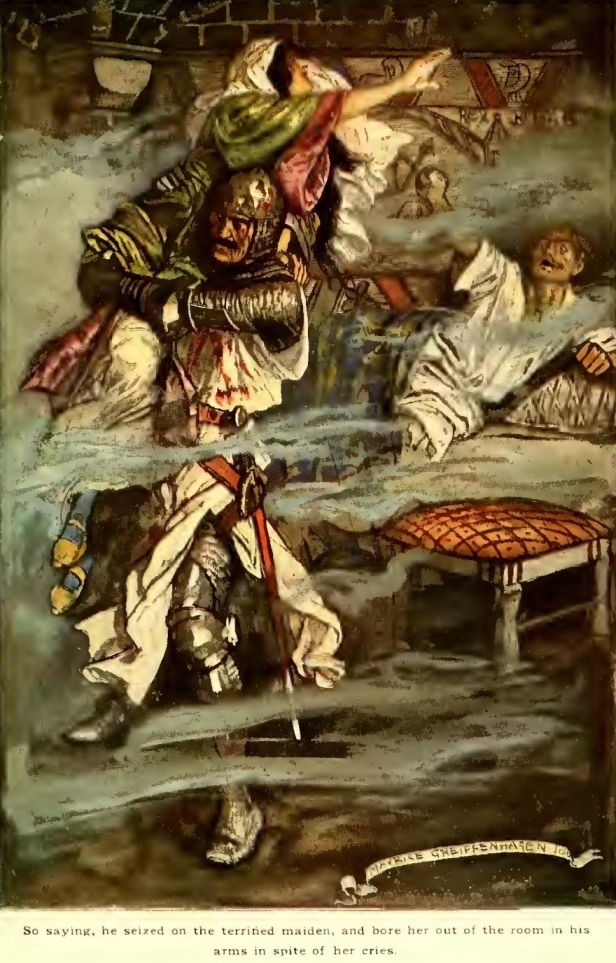
\includegraphics[height=.9\textheight]{ivanhoe/0403m}
    \caption{So saying, he seized on the terrified maiden, and bore her
    out of the room in his arms in spite of her cries.}
\end{figure}

``I had not found thee, Wilfred,'' said the Black Knight, who at that
instant entered the apartment, ``but for thy shouts.''

``If thou be'st true knight,'' said Wilfred, ``think not of me--pursue
yon ravisher--save the Lady Rowena--look to the noble Cedric!''

``In their turn,'' answered he of the Fetterlock, ``but thine is
first.''

And seizing upon Ivanhoe, he bore him off with as much ease as the
Templar had carried off Rebecca, rushed with him to the postern, and
having there delivered his burden to the care of two yeomen, he again
entered the castle to assist in the rescue of the other prisoners.

One turret was now in bright flames, which flashed out furiously from
window and shot-hole. But in other parts, the great thickness of the
walls and the vaulted roofs of the apartments, resisted the progress of
the flames, and there the rage of man still triumphed, as the scarce
more dreadful element held mastery elsewhere; for the besiegers pursued
the defenders of the castle from chamber to chamber, and satiated in
their blood the vengeance which had long animated them against the
soldiers of the tyrant Front-de-Boeuf. Most of the garrison resisted to
the uttermost--few of them asked quarter--none received it. The air was
filled with groans and clashing of arms--the floors were slippery with
the blood of despairing and expiring wretches.

Through this scene of confusion, Cedric rushed in quest of Rowena, while
the faithful Gurth, following him closely through the ``melee'',
neglected his own safety while he strove to avert the blows that were
aimed at his master. The noble Saxon was so fortunate as to reach his
ward's apartment just as she had abandoned all hope of safety, and, with
a crucifix clasped in agony to her bosom, sat in expectation of instant
death. He committed her to the charge of Gurth, to be conducted in
safety to the barbican, the road to which was now cleared of the enemy,
and not yet interrupted by the flames. This accomplished, the loyal
Cedric hastened in quest of his friend Athelstane, determined, at every
risk to himself, to save that last scion of Saxon royalty. But ere
Cedric penetrated as far as the old hall in which he had himself been a
prisoner, the inventive genius of Wamba had procured liberation for
himself and his companion in adversity.

When the noise of the conflict announced that it was at the hottest, the
Jester began to shout, with the utmost power of his lungs, ``Saint
George and the dragon!--Bonny Saint George for merry England!--The
castle is won!'' And these sounds he rendered yet more fearful, by
banging against each other two or three pieces of rusty armour which lay
scattered around the hall.

A guard, which had been stationed in the outer, or anteroom, and whose
spirits were already in a state of alarm, took fright at Wamba's
clamour, and, leaving the door open behind them, ran to tell the Templar
that foemen had entered the old hall. Meantime the prisoners found no
difficulty in making their escape into the anteroom, and from thence
into the court of the castle, which was now the last scene of contest.
Here sat the fierce Templar, mounted on horseback, surrounded by several
of the garrison both on horse and foot, who had united their strength to
that of this renowned leader, in order to secure the last chance of
safety and retreat which remained to them. The drawbridge had been
lowered by his orders, but the passage was beset; for the archers, who
had hitherto only annoyed the castle on that side by their missiles, no
sooner saw the flames breaking out, and the bridge lowered, than they
thronged to the entrance, as well to prevent the escape of the garrison,
as to secure their own share of booty ere the castle should be burnt
down. On the other hand, a party of the besiegers who had entered by the
postern were now issuing out into the court-yard, and attacking with
fury the remnant of the defenders who were thus assaulted on both sides
at once.

Animated, however, by despair, and supported by the example of their
indomitable leader, the remaining soldiers of the castle fought with the
utmost valour; and, being well-armed, succeeded more than once in
driving back the assailants, though much inferior in numbers. Rebecca,
placed on horseback before one of the Templar's Saracen slaves, was in
the midst of the little party; and Bois-Guilbert, notwithstanding the
confusion of the bloody fray, showed every attention to her safety.
Repeatedly he was by her side, and, neglecting his own defence, held
before her the fence of his triangular steel-plated shield; and anon
starting from his position by her, he cried his war-cry, dashed forward,
struck to earth the most forward of the assailants, and was on the same
instant once more at her bridle rein.

Athelstane, who, as the reader knows, was slothful, but not cowardly,
beheld the female form whom the Templar protected thus sedulously, and
doubted not that it was Rowena whom the knight was carrying off, in
despite of all resistance which could be offered.

``By the soul of Saint Edward,'' he said, ``I will rescue her from
yonder over-proud knight, and he shall die by my hand!''

``Think what you do!'' cried Wamba; ``hasty hand catches frog for
fish--by my bauble, yonder is none of my Lady Rowena--see but her long
dark locks!--Nay, an ye will not know black from white, ye may be
leader, but I will be no follower--no bones of mine shall be broken
unless I know for whom.--And you without armour too!--Bethink you, silk
bonnet never kept out steel blade.--Nay, then, if wilful will to water,
wilful must drench.--`Deus vobiscum', most doughty Athelstane!''--he
concluded, loosening the hold which he had hitherto kept upon the
Saxon's tunic.

To snatch a mace from the pavement, on which it lay beside one whose
dying grasp had just relinquished it--to rush on the Templar's band, and
to strike in quick succession to the right and left, levelling a warrior
at each blow, was, for Athelstane's great strength, now animated with
unusual fury, but the work of a single moment; he was soon within two
yards of Bois-Guilbert, whom he defied in his loudest tone.

``Turn, false-hearted Templar! let go her whom thou art unworthy to
touch--turn, limb of a hand of murdering and hypocritical robbers!''

``Dog!'' said the Templar, grinding his teeth, ``I will teach thee to
blaspheme the holy Order of the Temple of Zion;'' and with these words,
half-wheeling his steed, he made a demi-courbette towards the Saxon, and
rising in the stirrups, so as to take full advantage of the descent of
the horse, he discharged a fearful blow upon the head of Athelstane.

Well said Wamba, that silken bonnet keeps out no steel blade. So
trenchant was the Templar's weapon, that it shore asunder, as it had
been a willow twig, the tough and plaited handle of the mace, which the
ill-fated Saxon reared to parry the blow, and, descending on his head,
levelled him with the earth.

``\,`Ha! Beau-seant!'\,'' exclaimed Bois-Guilbert, ``thus be it to the
maligners of the Temple-knights!'' Taking advantage of the dismay which
was spread by the fall of Athelstane, and calling aloud, ``Those who
would save themselves, follow me!'' he pushed across the drawbridge,
dispersing the archers who would have intercepted them. He was followed
by his Saracens, and some five or six men-at-arms, who had mounted their
horses. The Templar's retreat was rendered perilous by the numbers of
arrows shot off at him and his party; but this did not prevent him from
galloping round to the barbican, of which, according to his previous
plan, he supposed it possible De Bracy might have been in possession.

``De Bracy! De Bracy!'' he shouted, ``art thou there?''

``I am here,'' replied De Bracy, ``but I am a prisoner.''

``Can I rescue thee?'' cried Bois-Guilbert.

``No,'' replied De Bracy; ``I have rendered me, rescue or no rescue. I
will be true prisoner. Save thyself--there are hawks abroad--put the
seas betwixt you and England--I dare not say more.''

``Well,'' answered the Templar, ``an thou wilt tarry there, remember I
have redeemed word and glove. Be the hawks where they will, methinks the
walls of the Preceptory of Templestowe will be cover sufficient, and
thither will I, like heron to her haunt.''

Having thus spoken, he galloped off with his followers.

Those of the castle who had not gotten to horse, still continued to
fight desperately with the besiegers, after the departure of the
Templar, but rather in despair of quarter than that they entertained any
hope of escape. The fire was spreading rapidly through all parts of the
castle, when Ulrica, who had first kindled it, appeared on a turret, in
the guise of one of the ancient furies, yelling forth a war-song, such
as was of yore raised on the field of battle by the scalds of the yet
heathen Saxons. Her long dishevelled grey hair flew back from her
uncovered head; the inebriating delight of gratified vengeance contended
in her eyes with the fire of insanity; and she brandished the distaff
which she held in her hand, as if she had been one of the Fatal Sisters,
who spin and abridge the thread of human life. Tradition has preserved
some wild strophes of the barbarous hymn which she chanted wildly amid
that scene of fire and of slaughter:--

\begin{verse}
\flagverse{1.}
Whet the bright steel,\\
Sons of the White Dragon!\\
Kindle the torch,\\
Daughter of Hengist!\\
The steel glimmers not for the carving of the banquet,\\
It is hard, broad, and sharply pointed;\\
The torch goeth not to the bridal chamber,\\
It steams and glitters blue with sulphur.\\
Whet the steel, the raven croaks!\\
Light the torch, Zernebock is yelling!\\
Whet the steel, sons of the Dragon!\\
Kindle the torch, daughter of Hengist! \\!
\flagverse{2.}
The black cloud is low over the thane's castle\\
The eagle screams--he rides on its bosom.\\
Scream not, grey rider of the sable cloud,\\
Thy banquet is prepared!\\
The maidens of Valhalla look forth,\\
The race of Hengist will send them guests.\\
Shake your black tresses, maidens of Valhalla!\\
And strike your loud timbrels for joy!\\
Many a haughty step bends to your halls,\\
Many a helmed head.\\!
\flagverse{3.}
Dark sits the evening upon the thanes castle,\\
The black clouds gather round;\\
Soon shall they be red as the blood of the valiant!\\
The destroyer of forests shall shake his red crest against
them.\\
He, the bright consumer of palaces,\\
Broad waves he his blazing banner,\\
Red, wide and dusky,\\
Over the strife of the valiant:\\
His joy is in the clashing swords and broken bucklers;\\
He loves to lick the hissing blood as it bursts warm from the
wound!\\!
\flagverse{4.}
All must perish!\\
The sword cleaveth the helmet;\\
The strong armour is pierced by the lance;\\
Fire devoureth the dwelling of princes,\\
Engines break down the fences of the battle.\\
All must perish!\\
The race of Hengist is gone--\\
The name of Horsa is no more!\\
Shrink not then from your doom, sons of the sword!\\
Let your blades drink blood like wine;\\
Feast ye in the banquet of slaughter,\\
By the light of the blazing halls!\\
Strong be your swords while your blood is warm,\\
And spare neither for pity nor fear,\\
For vengeance hath but an hour;\\
Strong hate itself shall expire\\
I also must perish!\footnote{Note G. Ulrica's Death Song. See
page~\pageref{noteCXXXI}.}\\!
\end{verse}

The towering flames had now surmounted every obstruction, and rose to
the evening skies one huge and burning beacon, seen far and wide through
the adjacent country. Tower after tower crashed down, with blazing roof
and rafter; and the combatants were driven from the court-yard. The
vanquished, of whom very few remained, scattered and escaped into the
neighbouring wood. The victors, assembling in large bands, gazed with
wonder, not unmixed with fear, upon the flames, in which their own ranks
and arms glanced dusky red. The maniac figure of the Saxon Ulrica was
for a long time visible on the lofty stand she had chosen, tossing her
arms abroad with wild exultation, as if she reined empress of the
conflagration which she had raised. At length, with a terrific crash,
the whole turret gave way, and she perished in the flames which had
consumed her tyrant. An awful pause of horror silenced each murmur of
the armed spectators, who, for the space of several minutes, stirred not
a finger, save to sign the cross. The voice of Locksley was then heard,
``Shout, yeomen!--the den of tyrants is no more! Let each bring his
spoil to our chosen place of rendezvous at the Trysting-tree in the
Harthill-walk; for there at break of day will we make just partition
among our own bands, together with our worthy allies in this great deed
of vengeance.''

    \chapter{Chapter XXXII}

\begin{verse}
Trust me each state must have its policies:\\
Kingdoms have edicts, cities have their charters;\\
Even the wild outlaw, in his forest-walk,\\
Keeps yet some touch of civil discipline;\\
For not since Adam wore his verdant apron,\\
Hath man with man in social union dwelt,\\
But laws were made to draw that union closer.\\!
\attrib{--Old Play}
\end{verse}

\lettrine{T}{he} daylight had dawned upon the glades of the oak forest.
The green
boughs glittered with all their pearls of dew. The hind led her fawn
from the covert of high fern to the more open walks of the greenwood,
and no huntsman was there to watch or intercept the stately hart, as he
paced at the head of the antler'd herd.

The outlaws were all assembled around the Trysting-tree in the
Harthill-walk, where they had spent the night in refreshing themselves
after the fatigues of the siege, some with wine, some with slumber, many
with hearing and recounting the events of the day, and computing the
heaps of plunder which their success had placed at the disposal of their
Chief.

The spoils were indeed very large; for, notwithstanding that much was
consumed, a great deal of plate, rich armour, and splendid clothing, had
been secured by the exertions of the dauntless outlaws, who could be
appalled by no danger when such rewards were in view. Yet so strict were
the laws of their society, that no one ventured to appropriate any part
of the booty, which was brought into one common mass, to be at the
disposal of their leader.

The place of rendezvous was an aged oak; not however the same to which
Locksley had conducted Gurth and Wamba in the earlier part of the story,
but one which was the centre of a silvan amphitheatre, within half a
mile of the demolished castle of Torquilstone. Here Locksley assumed his
seat--a throne of turf erected under the twisted branches of the huge
oak, and the silvan followers were gathered around him. He assigned to
the Black Knight a seat at his right hand, and to Cedric a place upon
his left.

``Pardon my freedom, noble sirs,'' he said, ``but in these glades I am
monarch--they are my kingdom; and these my wild subjects would reck but
little of my power, were I, within my own dominions, to yield place to
mortal man.--Now, sirs, who hath seen our chaplain? where is our curtal
Friar? A mass amongst Christian men best begins a busy morning.''--No
one had seen the Clerk of Copmanhurst. ``Over gods forbode!'' said the
outlaw chief, ``I trust the jolly priest hath but abidden by the
wine-pot a thought too late. Who saw him since the castle was ta'en?''

``I,'' quoth the Miller, ``marked him busy about the door of a cellar,
swearing by each saint in the calendar he would taste the smack of
Front-de-Boeuf's Gascoigne wine.''

``Now, the saints, as many as there be of them,'' said the Captain,
``forefend, lest he has drunk too deep of the wine-butts, and perished
by the fall of the castle!--Away, Miller!--take with you enow of men,
seek the place where you last saw him--throw water from the moat on the
scorching ruins--I will have them removed stone by stone ere I lose my
curtal Friar.''

The numbers who hastened to execute this duty, considering that an
interesting division of spoil was about to take place, showed how much
the troop had at heart the safety of their spiritual father.

``Meanwhile, let us proceed,'' said Locksley; ``for when this bold deed
shall be sounded abroad, the bands of De Bracy, of Malvoisin, and other
allies of Front-de-Boeuf, will be in motion against us, and it were well
for our safety that we retreat from the vicinity.--Noble Cedric,'' he
said, turning to the Saxon, ``that spoil is divided into two portions;
do thou make choice of that which best suits thee, to recompense thy
people who were partakers with us in this adventure.''

``Good yeoman,'' said Cedric, ``my heart is oppressed with sadness. The
noble Athelstane of Coningsburgh is no more--the last sprout of the
sainted Confessor! Hopes have perished with him which can never
return!--A sparkle hath been quenched by his blood, which no human
breath can again rekindle! My people, save the few who are now with me,
do but tarry my presence to transport his honoured remains to their last
mansion. The Lady Rowena is desirous to return to Rotherwood, and must
be escorted by a sufficient force. I should, therefore, ere now, have
left this place; and I waited--not to share the booty, for, so help me
God and Saint Withold! as neither I nor any of mine will touch the value
of a liard,--I waited but to render my thanks to thee and to thy bold
yeomen, for the life and honour ye have saved.''

``Nay, but,'' said the chief Outlaw, ``we did but half the work at
most--take of the spoil what may reward your own neighbours and
followers.''

``I am rich enough to reward them from mine own wealth,'' answered
Cedric.

``And some,'' said Wamba, ``have been wise enough to reward themselves;
they do not march off empty-handed altogether. We do not all wear
motley.''

``They are welcome,'' said Locksley; ``our laws bind none but
ourselves.''

``But, thou, my poor knave,'' said Cedric, turning about and embracing
his Jester, ``how shall I reward thee, who feared not to give thy body
to chains and death instead of mine!--All forsook me, when the poor fool
was faithful!''

A tear stood in the eye of the rough Thane as he spoke--a mark of
feeling which even the death of Athelstane had not extracted; but there
was something in the half-instinctive attachment of his clown, that
waked his nature more keenly than even grief itself.

``Nay,'' said the Jester, extricating himself from master's caress, ``if
you pay my service with the water of your eye, the Jester must weep for
company, and then what becomes of his vocation?--But, uncle, if you
would indeed pleasure me, I pray you to pardon my playfellow Gurth, who
stole a week from your service to bestow it on your son.''

``Pardon him!'' exclaimed Cedric; ``I will both pardon and reward
him.--Kneel down, Gurth.''--The swineherd was in an instant at his
master's feet--``\textsc{theow} and \textsc{esne}\footnote{Thrall and
bondsman.} art thou no longer,'' said
Cedric touching him with a wand; ``\textsc{folkfree} and
\textsc{sacless}\footnote{A lawful freeman.} art
thou in town and from town, in the forest as in the field. A hide of
land I give to thee in my steads of Walbrugham, from me and mine to thee
and thine aye and for ever; and God's malison on his head who this
gainsays!''

No longer a serf, but a freeman and a landholder, Gurth sprung upon his
feet, and twice bounded aloft to almost his own height from the ground.
``A smith and a file,'' he cried, ``to do away the collar from the neck
of a freeman!--Noble master! doubled is my strength by your gift, and
doubly will I fight for you!--There is a free spirit in my breast--I am
a man changed to myself and all around.--Ha, Fangs!'' he continued,--for
that faithful cur, seeing his master thus transported, began to jump
upon him, to express his sympathy,--``knowest thou thy master still?''

``Ay,'' said Wamba, ``Fangs and I still know thee, Gurth, though we must
needs abide by the collar; it is only thou art likely to forget both us
and thyself.''

``I shall forget myself indeed ere I forget thee, true comrade,'' said
Gurth; ``and were freedom fit for thee, Wamba, the master would not let
thee want it.''

``Nay,'' said Wamba, ``never think I envy thee, brother Gurth; the serf
sits by the hall-fire when the freeman must forth to the field of
battle--And what saith Oldhelm of Malmsbury--Better a fool at a feast
than a wise man at a fray.''

The tramp of horses was now heard, and the Lady Rowena appeared,
surrounded by several riders, and a much stronger party of footmen, who
joyfully shook their pikes and clashed their brown-bills for joy of her
freedom. She herself, richly attired, and mounted on a dark chestnut
palfrey, had recovered all the dignity of her manner, and only an
unwonted degree of paleness showed the sufferings she had undergone. Her
lovely brow, though sorrowful, bore on it a cast of reviving hope for
the future, as well as of grateful thankfulness for the past
deliverance--She knew that Ivanhoe was safe, and she knew that
Athelstane was dead. The former assurance filled her with the most
sincere delight; and if she did not absolutely rejoice at the latter,
she might be pardoned for feeling the full advantage of being freed from
further persecution on the only subject in which she had ever been
contradicted by her guardian Cedric.

As Rowena bent her steed towards Locksley's seat, that bold yeoman, with
all his followers, rose to receive her, as if by a general instinct of
courtesy. The blood rose to her cheeks, as, courteously waving her hand,
and bending so low that her beautiful and loose tresses were for an
instant mixed with the flowing mane of her palfrey, she expressed in few
but apt words her obligations and her gratitude to Locksley and her
other deliverers.--``God bless you, brave men,'' she concluded, ``God
and Our Lady bless you and requite you for gallantly perilling
yourselves in the cause of the oppressed!--If any of you should hunger,
remember Rowena has food--if you should thirst, she has many a butt of
wine and brown ale--and if the Normans drive ye from these walks, Rowena
has forests of her own, where her gallant deliverers may range at full
freedom, and never ranger ask whose arrow hath struck down the deer.''

``Thanks, gentle lady,'' said Locksley; ``thanks from my company and
myself. But, to have saved you requites itself. We who walk the
greenwood do many a wild deed, and the Lady Rowena's deliverance may be
received as an atonement.''

Again bowing from her palfrey, Rowena turned to depart; but pausing a
moment, while Cedric, who was to attend her, was also taking his leave,
she found herself unexpectedly close by the prisoner De Bracy. He stood
under a tree in deep meditation, his arms crossed upon his breast, and
Rowena was in hopes she might pass him unobserved. He looked up,
however, and, when aware of her presence, a deep flush of shame suffused
his handsome countenance. He stood a moment most irresolute; then,
stepping forward, took her palfrey by the rein, and bent his knee before
her.

``Will the Lady Rowena deign to cast an eye--on a captive knight--on a
dishonoured soldier?''

``Sir Knight,'' answered Rowena, ``in enterprises such as yours, the
real dishonour lies not in failure, but in success.''

``Conquest, lady, should soften the heart,'' answered De Bracy; ``let me
but know that the Lady Rowena forgives the violence occasioned by an
ill-fated passion, and she shall soon learn that De Bracy knows how to
serve her in nobler ways.''

``I forgive you, Sir Knight,'' said Rowena, ``as a Christian.''

``That means,'' said Wamba, ``that she does not forgive him at all.''

``But I can never forgive the misery and desolation your madness has
occasioned,'' continued Rowena.

``Unloose your hold on the lady's rein,'' said Cedric, coming up. ``By
the bright sun above us, but it were shame, I would pin thee to the
earth with my javelin--but be well assured, thou shalt smart, Maurice de
Bracy, for thy share in this foul deed.''

``He threatens safely who threatens a prisoner,'' said De Bracy; ``but
when had a Saxon any touch of courtesy?''

Then retiring two steps backward, he permitted the lady to move on.

Cedric, ere they departed, expressed his peculiar gratitude to the Black
Champion, and earnestly entreated him to accompany him to Rotherwood.

``I know,'' he said, ``that ye errant knights desire to carry your
fortunes on the point of your lance, and reck not of land or goods; but
war is a changeful mistress, and a home is sometimes desirable even to
the champion whose trade is wandering. Thou hast earned one in the halls
of Rotherwood, noble knight. Cedric has wealth enough to repair the
injuries of fortune, and all he has is his deliverer's--Come, therefore,
to Rotherwood, not as a guest, but as a son or brother.''

``Cedric has already made me rich,'' said the Knight,--``he has taught
me the value of Saxon virtue. To Rotherwood will I come, brave Saxon,
and that speedily; but, as now, pressing matters of moment detain me
from your halls. Peradventure when I come hither, I will ask such a boon
as will put even thy generosity to the test.''

``It is granted ere spoken out,'' said Cedric, striking his ready hand
into the gauntleted palm of the Black Knight,--``it is granted already,
were it to affect half my fortune.''

``Gage not thy promise so lightly,'' said the Knight of the Fetterlock;
``yet well I hope to gain the boon I shall ask. Meanwhile, adieu.''

``I have but to say,'' added the Saxon, ``that, during the funeral rites
of the noble Athelstane, I shall be an inhabitant of the halls of his
castle of Coningsburgh--They will be open to all who choose to partake
of the funeral banqueting; and, I speak in name of the noble Edith,
mother of the fallen prince, they will never be shut against him who
laboured so bravely, though unsuccessfully, to save Athelstane from
Norman chains and Norman steel.''

``Ay, ay,'' said Wamba, who had resumed his attendance on his master,
``rare feeding there will be--pity that the noble Athelstane cannot
banquet at his own funeral.--But he,'' continued the Jester, lifting up
his eyes gravely, ``is supping in Paradise, and doubtless does honour to
the cheer.''

``Peace, and move on,'' said Cedric, his anger at this untimely jest
being checked by the recollection of Wamba's recent services. Rowena
waved a graceful adieu to him of the Fetterlock--the Saxon bade God
speed him, and on they moved through a wide glade of the forest.

They had scarce departed, ere a sudden procession moved from under the
greenwood branches, swept slowly round the silvan amphitheatre, and took
the same direction with Rowena and her followers. The priests of a
neighbouring convent, in expectation of the ample donation, or
``soul-scat'', which Cedric had propined, attended upon the car in which
the body of Athelstane was laid, and sang hymns as it was sadly and
slowly borne on the shoulders of his vassals to his castle of
Coningsburgh, to be there deposited in the grave of Hengist, from whom
the deceased derived his long descent. Many of his vassals had assembled
at the news of his death, and followed the bier with all the external
marks, at least, of dejection and sorrow. Again the outlaws arose, and
paid the same rude and spontaneous homage to death, which they had so
lately rendered to beauty--the slow chant and mournful step of the
priests brought back to their remembrance such of their comrades as had
fallen in the yesterday's array. But such recollections dwell not long
with those who lead a life of danger and enterprise, and ere the sound
of the death-hymn had died on the wind, the outlaws were again busied in
the distribution of their spoil.

``Valiant knight,'' said Locksley to the Black Champion, ``without whose
good heart and mighty arm our enterprise must altogether have failed,
will it please you to take from that mass of spoil whatever may best
serve to pleasure you, and to remind you of this my Trysting-tree?''

``I accept the offer,'' said the Knight, ``as frankly as it is given;
and I ask permission to dispose of Sir Maurice de Bracy at my own
pleasure.''

``He is thine already,'' said Locksley, ``and well for him! else the
tyrant had graced the highest bough of this oak, with as many of his
Free-Companions as we could gather, hanging thick as acorns around
him.--But he is thy prisoner, and he is safe, though he had slain my
father.''

``De Bracy,'' said the Knight, ``thou art free--depart. He whose
prisoner thou art scorns to take mean revenge for what is past. But
beware of the future, lest a worse thing befall thee.--Maurice de Bracy,
I say BEWARE!''

De Bracy bowed low and in silence, and was about to withdraw, when the
yeomen burst at once into a shout of execration and derision. The proud
knight instantly stopped, turned back, folded his arms, drew up his form
to its full height, and exclaimed, ``Peace, ye yelping curs! who open
upon a cry which ye followed not when the stag was at bay--De Bracy
scorns your censure as he would disdain your applause. To your brakes
and caves, ye outlawed thieves! and be silent when aught knightly or
noble is but spoken within a league of your fox-earths.''

This ill-timed defiance might have procured for De Bracy a volley of
arrows, but for the hasty and imperative interference of the outlaw
Chief. Meanwhile the knight caught a horse by the rein, for several
which had been taken in the stables of Front-de-Boeuf stood accoutred
around, and were a valuable part of the booty. He threw himself upon the
saddle, and galloped off through the wood.

When the bustle occasioned by this incident was somewhat composed, the
chief Outlaw took from his neck the rich horn and baldric which he had
recently gained at the strife of archery near Ashby.

``Noble knight.'' he said to him of the Fetterlock, ``if you disdain not
to grace by your acceptance a bugle which an English yeoman has once
worn, this I will pray you to keep as a memorial of your gallant
bearing--and if ye have aught to do, and, as happeneth oft to a gallant
knight, ye chance to be hard bested in any forest between Trent and
Tees, wind three mots\footnote{The notes upon the bugle were anciently
called mots, and
are distinguished in the old treatises on hunting, not by musical
characters, but by written words.} upon the horn thus, `Wa-sa-hoa!' and it
may well chance ye shall find helpers and rescue.''

He then gave breath to the bugle, and winded once and again the call
which he described, until the knight had caught the notes.

``Gramercy for the gift, bold yeoman,'' said the Knight; ``and better
help than thine and thy rangers would I never seek, were it at my utmost
need.'' And then in his turn he winded the call till all the greenwood
rang.

``Well blown and clearly,'' said the yeoman; ``beshrew me an thou
knowest not as much of woodcraft as of war!--thou hast been a striker of
deer in thy day, I warrant.--Comrades, mark these three mots--it is the
call of the Knight of the Fetterlock; and he who hears it, and hastens
not to serve him at his need, I will have him scourged out of our band
with his own bowstring.''

``Long live our leader!'' shouted the yeomen, ``and long live the Black
Knight of the Fetterlock!--May he soon use our service, to prove how
readily it will be paid.''

Locksley now proceeded to the distribution of the spoil, which he
performed with the most laudable impartiality. A tenth part of the whole
was set apart for the church, and for pious uses; a portion was next
allotted to a sort of public treasury; a part was assigned to the widows
and children of those who had fallen, or to be expended in masses for
the souls of such as had left no surviving family. The rest was divided
amongst the outlaws, according to their rank and merit, and the judgment
of the Chief, on all such doubtful questions as occurred, was delivered
with great shrewdness, and received with absolute submission. The Black
Knight was not a little surprised to find that men, in a state so
lawless, were nevertheless among themselves so regularly and equitably
governed, and all that he observed added to his opinion of the justice
and judgment of their leader.

When each had taken his own proportion of the booty, and while the
treasurer, accompanied by four tall yeomen, was transporting that
belonging to the state to some place of concealment or of security, the
portion devoted to the church still remained unappropriated.

``I would,'' said the leader, ``we could hear tidings of our joyous
chaplain--he was never wont to be absent when meat was to be blessed, or
spoil to be parted; and it is his duty to take care of these the tithes
of our successful enterprise. It may be the office has helped to cover
some of his canonical irregularities. Also, I have a holy brother of his
a prisoner at no great distance, and I would fain have the Friar to help
me to deal with him in due sort--I greatly misdoubt the safety of the
bluff priest.''

``I were right sorry for that,'' said the Knight of the Fetterlock,
``for I stand indebted to him for the joyous hospitality of a merry
night in his cell. Let us to the ruins of the castle; it may be we shall
there learn some tidings of him.''

While they thus spoke, a loud shout among the yeomen announced the
arrival of him for whom they feared, as they learned from the stentorian
voice of the Friar himself, long before they saw his burly person.

``Make room, my merry-men!'' he exclaimed; ``room for your godly father
and his prisoner--Cry welcome once more.--I come, noble leader, like an
eagle with my prey in my clutch.''--And making his way through the ring,
amidst the laughter of all around, he appeared in majestic triumph, his
huge partisan in one hand, and in the other a halter, one end of which
was fastened to the neck of the unfortunate Isaac of York, who, bent
down by sorrow and terror, was dragged on by the victorious priest, who
shouted aloud, ``Where is Allan-a-Dale, to chronicle me in a ballad, or
if it were but a lay?--By Saint Hermangild, the jingling crowder is ever
out of the way where there is an apt theme for exalting valour!''

``Curtal Priest,'' said the Captain, ``thou hast been at a wet mass this
morning, as early as it is. In the name of Saint Nicholas, whom hast
thou got here?''

``A captive to my sword and to my lance, noble Captain,'' replied the
Clerk of Copmanhurst; ``to my bow and to my halberd, I should rather
say; and yet I have redeemed him by my divinity from a worse captivity.
Speak, Jew--have I not ransomed thee from Sathanas?--have I not taught
thee thy `credo', thy `pater', and thine `Ave Maria'?--Did I not spend
the whole night in drinking to thee, and in expounding of mysteries?''

``For the love of God!'' ejaculated the poor Jew, ``will no one take me
out of the keeping of this mad--I mean this holy man?''

``How's this, Jew?'' said the Friar, with a menacing aspect; ``dost thou
recant, Jew?--Bethink thee, if thou dost relapse into thine infidelity,
though thou are not so tender as a suckling pig--I would I had one to
break my fast upon--thou art not too tough to be roasted! Be
conformable, Isaac, and repeat the words after me. `Ave Maria'!--''

``Nay, we will have no profanation, mad Priest,'' said Locksley; ``let
us rather hear where you found this prisoner of thine.''

``By Saint Dunstan,'' said the Friar, ``I found him where I sought for
better ware! I did step into the cellarage to see what might be rescued
there; for though a cup of burnt wine, with spice, be an evening's
drought for an emperor, it were waste, methought, to let so much good
liquor be mulled at once; and I had caught up one runlet of sack, and
was coming to call more aid among these lazy knaves, who are ever to
seek when a good deed is to be done, when I was avised of a strong
door--Aha! thought I, here is the choicest juice of all in this secret
crypt; and the knave butler, being disturbed in his vocation, hath left
the key in the door--In therefore I went, and found just nought besides
a commodity of rusted chains and this dog of a Jew, who presently
rendered himself my prisoner, rescue or no rescue. I did but refresh
myself after the fatigue of the action, with the unbeliever, with one
humming cup of sack, and was proceeding to lead forth my captive, when,
crash after crash, as with wild thunder-dint and levin-fire, down
toppled the masonry of an outer tower, (marry beshrew their hands that
built it not the firmer!) and blocked up the passage. The roar of one
falling tower followed another--I gave up thought of life; and deeming
it a dishonour to one of my profession to pass out of this world in
company with a Jew, I heaved up my halberd to beat his brains out; but I
took pity on his grey hairs, and judged it better to lay down the
partisan, and take up my spiritual weapon for his conversion. And truly,
by the blessing of Saint Dunstan, the seed has been sown in good soil;
only that, with speaking to him of mysteries through the whole night,
and being in a manner fasting, (for the few droughts of sack which I
sharpened my wits with were not worth marking,) my head is well-nigh
dizzied, I trow.--But I was clean exhausted.--Gilbert and Wibbald know
in what state they found me--quite and clean exhausted.''

``We can bear witness,'' said Gilbert; ``for when we had cleared away
the ruin, and by Saint Dunstan's help lighted upon the dungeon stair, we
found the runlet of sack half empty, the Jew half dead, and the Friar
more than half--exhausted, as he calls it.''

``Ye be knaves! ye lie!'' retorted the offended Friar; ``it was you and
your gormandizing companions that drank up the sack, and called it your
morning draught--I am a pagan, an I kept it not for the Captain's own
throat. But what recks it? The Jew is converted, and understands all I
have told him, very nearly, if not altogether, as well as myself.''

``Jew,'' said the Captain, ``is this true? hast thou renounced thine
unbelief?''

``May I so find mercy in your eyes,'' said the Jew, ``as I know not one
word which the reverend prelate spake to me all this fearful night.
Alas! I was so distraught with agony, and fear, and grief, that had our
holy father Abraham come to preach to me, he had found but a deaf
listener.''

``Thou liest, Jew, and thou knowest thou dost.'' said the Friar; ``I
will remind thee of but one word of our conference--thou didst promise
to give all thy substance to our holy Order.''

``So help me the Promise, fair sirs,'' said Isaac, even more alarmed
than before, ``as no such sounds ever crossed my lips! Alas! I am an
aged beggar'd man--I fear me a childless--have ruth on me, and let me
go!''

``Nay,'' said the Friar, ``if thou dost retract vows made in favour of
holy Church, thou must do penance.''

Accordingly, he raised his halberd, and would have laid the staff of it
lustily on the Jew's shoulders, had not the Black Knight stopped the
blow, and thereby transferred the Holy Clerk's resentment to himself.

``By Saint Thomas of Kent,'' said he, ``an I buckle to my gear, I will
teach thee, sir lazy lover, to mell with thine own matters, maugre thine
iron case there!''

``Nay, be not wroth with me,'' said the Knight; ``thou knowest I am thy
sworn friend and comrade.''

``I know no such thing,'' answered the Friar; ``and defy thee for a
meddling coxcomb!''

``Nay, but,'' said the Knight, who seemed to take a pleasure in
provoking his quondam host, ``hast thou forgotten how, that for my sake
(for I say nothing of the temptation of the flagon and the pasty) thou
didst break thy vow of fast and vigil?''

``Truly, friend,'' said the Friar, clenching his huge fist, ``I will
bestow a buffet on thee.''

``I accept of no such presents,'' said the Knight; ``I am content to
take thy cuff\footnote{Note H. Richard Coeur-de-Lion. See
page~\pageref{noteCXXXII}.} as a loan, but I will repay thee with usury as
deep as ever thy prisoner there exacted in his traffic.''

``I will prove that presently,'' said the Friar.

``Hola!'' cried the Captain, ``what art thou after, mad Friar? brawling
beneath our Trysting-tree?''

``No brawling,'' said the Knight, ``it is but a friendly interchange of
courtesy.--Friar, strike an thou darest--I will stand thy blow, if thou
wilt stand mine.''

``Thou hast the advantage with that iron pot on thy head,'' said the
churchman; ``but have at thee--Down thou goest, an thou wert Goliath of
Gath in his brazen helmet.''

The Friar bared his brawny arm up to the elbow, and putting his full
strength to the blow, gave the Knight a buffet that might have felled an
ox. But his adversary stood firm as a rock. A loud shout was uttered by
all the yeomen around; for the Clerk's cuff was proverbial amongst them,
and there were few who, in jest or earnest, had not had the occasion to
know its vigour.

``Now, Priest,'' said, the Knight, pulling off his gauntlet, ``if I had
vantage on my head, I will have none on my hand--stand fast as a true
man.''

``\,`Genam meam dedi vapulatori'--I have given my cheek to the smiter,''
said the Priest; ``an thou canst stir me from the spot, fellow, I will
freely bestow on thee the Jew's ransom.''

So spoke the burly Priest, assuming, on his part, high defiance. But who
may resist his fate? The buffet of the Knight was given with such
strength and good-will, that the Friar rolled head over heels upon the
plain, to the great amazement of all the spectators. But he arose
neither angry nor crestfallen.

``Brother,'' said he to the Knight, ``thou shouldst have used thy
strength with more discretion. I had mumbled but a lame mass an thou
hadst broken my jaw, for the piper plays ill that wants the nether
chops. Nevertheless, there is my hand, in friendly witness, that I will
exchange no more cuffs with thee, having been a loser by the barter. End
now all unkindness. Let us put the Jew to ransom, since the leopard will
not change his spots, and a Jew he will continue to be.''

``The Priest,'' said Clement, ``is not half so confident of the Jew's
conversion, since he received that buffet on the ear.''

``Go to, knave, what pratest thou of conversions?--what, is there no
respect?--all masters and no men?--I tell thee, fellow, I was somewhat
totty when I received the good knight's blow, or I had kept my ground
under it. But an thou gibest more of it, thou shalt learn I can give as
well as take.''

``Peace all!'' said the Captain. ``And thou, Jew, think of thy ransom;
thou needest not to be told that thy race are held to be accursed in all
Christian communities, and trust me that we cannot endure thy presence
among us. Think, therefore, of an offer, while I examine a prisoner of
another cast.''

``Were many of Front-de-Boeuf's men taken?'' demanded the Black Knight.

``None of note enough to be put to ransom,'' answered the Captain; ``a
set of hilding fellows there were, whom we dismissed to find them a new
master--enough had been done for revenge and profit; the bunch of them
were not worth a cardecu. The prisoner I speak of is better booty--a
jolly monk riding to visit his leman, an I may judge by his horse-gear
and wearing apparel.--Here cometh the worthy prelate, as pert as a
pyet.'' And, between two yeomen, was brought before the silvan throne of
the outlaw Chief, our old friend, Prior Aymer of Jorvaulx.

    \chapter{Chapter XXXIII}

\begin{verse}
---Flower of warriors,\\
How is't with Titus Lartius?\\
MARCIUS.--As with a man busied about decrees,\\
Condemning some to death and some to exile,\\
Ransoming him or pitying, threatening the other.\\!
\attrib{--Coriolanus}
\end{verse}

\lettrine{T}{he} captive Abbot's features and manners exhibited a
whimsical mixture
of offended pride, and deranged foppery and bodily terror.

``Why, how now, my masters?'' said he, with a voice in which all three
emotions were blended. ``What order is this among ye? Be ye Turks or
Christians, that handle a churchman?--Know ye what it is, `manus
imponere in servos Domini'? Ye have plundered my mails--torn my cope of
curious cut lace, which might have served a cardinal!--Another in my
place would have been at his `excommunicabo vos'; but I am placible, and
if ye order forth my palfreys, release my brethren, and restore my
mails, tell down with all speed an hundred crowns to be expended in
masses at the high altar of Jorvaulx Abbey, and make your vow to eat no
venison until next Pentecost, it may be you shall hear little more of
this mad frolic.''

``Holy Father,'' said the chief Outlaw, ``it grieves me to think that
you have met with such usage from any of my followers, as calls for your
fatherly reprehension.''

``Usage!'' echoed the priest, encouraged by the mild tone of the silvan
leader; ``it were usage fit for no hound of good race--much less for a
Christian--far less for a priest--and least of all for the Prior of the
holy community of Jorvaulx. Here is a profane and drunken minstrel,
called Allan-a-Dale--`nebulo quidam'--who has menaced me with corporal
punishment--nay, with death itself, an I pay not down four hundred
crowns of ransom, to the boot of all the treasure he hath already robbed
me of--gold chains and gymmal rings to an unknown value; besides what is
broken and spoiled among their rude hands, such as my pouncer-box and
silver crisping-tongs.''

``It is impossible that Allan-a-Dale can have thus treated a man of your
reverend bearing,'' replied the Captain.

``It is true as the gospel of Saint Nicodemus,'' said the Prior; ``he
swore, with many a cruel north-country oath, that he would hang me up on
the highest tree in the greenwood.''

``Did he so in very deed? Nay, then, reverend father, I think you had
better comply with his demands--for Allan-a-Dale is the very man to
abide by his word when he has so pledged it.''\footnote{A commissary is
said to have received similar
consolation from a certain Commander-in-chief, to whom he complained
that a general officer had used some such threat towards him as that in
the text.}

``You do but jest with me,'' said the astounded Prior, with a forced
laugh; ``and I love a good jest with all my heart. But, ha! ha! ha! when
the mirth has lasted the livelong night, it is time to be grave in the
morning.''

``And I am as grave as a father confessor,'' replied the Outlaw; ``you
must pay a round ransom, Sir Prior, or your convent is likely to be
called to a new election; for your place will know you no more.''

``Are ye Christians,'' said the Prior, ``and hold this language to a
churchman?''

``Christians! ay, marry are we, and have divinity among us to boot,''
answered the Outlaw. ``Let our buxom chaplain stand forth, and expound
to this reverend father the texts which concern this matter.''

The Friar, half-drunk, half-sober, had huddled a friar's frock over his
green cassock, and now summoning together whatever scraps of learning he
had acquired by rote in former days, ``Holy father,'' said he, ``\,`Deus
faciat salvam benignitatem vestram'--You are welcome to the greenwood.''

``What profane mummery is this?'' said the Prior. ``Friend, if thou
be'st indeed of the church, it were a better deed to show me how I may
escape from these men's hands, than to stand ducking and grinning here
like a morris-dancer.''

``Truly, reverend father,'' said the Friar, ``I know but one mode in
which thou mayst escape. This is Saint Andrew's day with us, we are
taking our tithes.''

``But not of the church, then, I trust, my good brother?'' said the
Prior.

``Of church and lay,'' said the Friar; ``and therefore, Sir Prior
`facite vobis amicos de Mammone iniquitatis'--make yourselves friends of
the Mammon of unrighteousness, for no other friendship is like to serve
your turn.''

``I love a jolly woodsman at heart,'' said the Prior, softening his
tone; ``come, ye must not deal too hard with me--I can well of
woodcraft, and can wind a horn clear and lustily, and hollo till every
oak rings again--Come, ye must not deal too hard with me.''

``Give him a horn,'' said the Outlaw; ``we will prove the skill he
boasts of.''

The Prior Aymer winded a blast accordingly. The Captain shook his head.

``Sir Prior,'' he said, ``thou blowest a merry note, but it may not
ransom thee--we cannot afford, as the legend on a good knight's shield
hath it, to set thee free for a blast. Moreover, I have found thee--thou
art one of those, who, with new French graces and Tra-li-ras, disturb
the ancient English bugle notes.--Prior, that last flourish on the
recheat hath added fifty crowns to thy ransom, for corrupting the true
old manly blasts of venerie.''

``Well, friend,'' said the Abbot, peevishly, ``thou art ill to please
with thy woodcraft. I pray thee be more conformable in this matter of my
ransom. At a word--since I must needs, for once, hold a candle to the
devil--what ransom am I to pay for walking on Watling-street, without
having fifty men at my back?''

``Were it not well,'' said the Lieutenant of the gang apart to the
Captain, ``that the Prior should name the Jew's ransom, and the Jew name
the Prior's?''

``Thou art a mad knave,'' said the Captain, ``but thy plan
transcends!--Here, Jew, step forth--Look at that holy Father Aymer,
Prior of the rich Abbey of Jorvaulx, and tell us at what ransom we
should hold him?--Thou knowest the income of his convent, I warrant
thee.''

``O, assuredly,'' said Isaac. ``I have trafficked with the good fathers,
and bought wheat and barley, and fruits of the earth, and also much
wool. O, it is a rich abbey-stede, and they do live upon the fat, and
drink the sweet wines upon the lees, these good fathers of Jorvaulx. Ah,
if an outcast like me had such a home to go to, and such incomings by
the year and by the month, I would pay much gold and silver to redeem my
captivity.''

``Hound of a Jew!'' exclaimed the Prior, ``no one knows better than thy
own cursed self, that our holy house of God is indebted for the
finishing of our chancel--''

``And for the storing of your cellars in the last season with the due
allowance of Gascon wine,'' interrupted the Jew; ``but that--that is
small matters.''

``Hear the infidel dog!'' said the churchman; ``he jangles as if our
holy community did come under debts for the wines we have a license to
drink, `propter necessitatem, et ad frigus depellendum'. The circumcised
villain blasphemeth the holy church, and Christian men listen and rebuke
him not!''

``All this helps nothing,'' said the leader.--``Isaac, pronounce what he
may pay, without flaying both hide and hair.''

``An six hundred crowns,'' said Isaac, ``the good Prior might well pay
to your honoured valours, and never sit less soft in his stall.''

``Six hundred crowns,'' said the leader, gravely; ``I am contented--thou
hast well spoken, Isaac--six hundred crowns.--It is a sentence, Sir
Prior.''

``A sentence!--a sentence!'' exclaimed the band; ``Solomon had not done
it better.''

``Thou hearest thy doom, Prior,'' said the leader.

``Ye are mad, my masters,'' said the Prior; ``where am I to find such a
sum? If I sell the very pyx and candlesticks on the altar at Jorvaulx, I
shall scarce raise the half; and it will be necessary for that purpose
that I go to Jorvaulx myself; ye may retain as borrows\footnote{Borghs,
or borrows, signifies pledges. Hence our word to
borrow, because we pledge ourselves to restore what is lent.} my two
priests.''

``That will be but blind trust,'' said the Outlaw; ``we will retain
thee, Prior, and send them to fetch thy ransom. Thou shalt not want a
cup of wine and a collop of venison the while; and if thou lovest
woodcraft, thou shalt see such as your north country never witnessed.''

``Or, if so please you,'' said Isaac, willing to curry favour with the
outlaws, ``I can send to York for the six hundred crowns, out of certain
monies in my hands, if so be that the most reverend Prior present will
grant me a quittance.''

``He shall grant thee whatever thou dost list, Isaac,'' said the
Captain; ``and thou shalt lay down the redemption money for Prior Aymer
as well as for thyself.''

``For myself! ah, courageous sirs,'' said the Jew, ``I am a broken and
impoverished man; a beggar's staff must be my portion through life,
supposing I were to pay you fifty crowns.''

``The Prior shall judge of that matter,'' replied the Captain.--``How
say you, Father Aymer? Can the Jew afford a good ransom?''

``Can he afford a ransom?'' answered the Prior ``Is he not Isaac of
York, rich enough to redeem the captivity of the ten tribes of Israel,
who were led into Assyrian bondage?--I have seen but little of him
myself, but our cellarer and treasurer have dealt largely with him, and
report says that his house at York is so full of gold and silver as is a
shame in any Christian land. Marvel it is to all living Christian hearts
that such gnawing adders should be suffered to eat into the bowels of
the state, and even of the holy church herself, with foul usuries and
extortions.''

``Hold, father,'' said the Jew, ``mitigate and assuage your choler. I
pray of your reverence to remember that I force my monies upon no one.
But when churchman and layman, prince and prior, knight and priest, come
knocking to Isaac's door, they borrow not his shekels with these uncivil
terms. It is then, Friend Isaac, will you pleasure us in this matter,
and our day shall be truly kept, so God sa' me?--and Kind Isaac, if ever
you served man, show yourself a friend in this need! And when the day
comes, and I ask my own, then what hear I but Damned Jew, and The curse
of Egypt on your tribe, and all that may stir up the rude and uncivil
populace against poor strangers!''

``Prior,'' said the Captain, ``Jew though he be, he hath in this spoken
well. Do thou, therefore, name his ransom, as he named thine, without
farther rude terms.''

``None but `latro famosus'--the interpretation whereof,'' said the
Prior, ``will I give at some other time and tide--would place a
Christian prelate and an unbaptized Jew upon the same bench. But since
ye require me to put a price upon this caitiff, I tell you openly that
ye will wrong yourselves if you take from him a penny under a thousand
crowns.''

``A sentence!--a sentence!'' exclaimed the chief Outlaw.

``A sentence!--a sentence!'' shouted his assessors; ``the Christian has
shown his good nurture, and dealt with us more generously than the
Jew.''

``The God of my fathers help me!'' said the Jew; ``will ye bear to the
ground an impoverished creature?--I am this day childless, and will ye
deprive me of the means of livelihood?''

``Thou wilt have the less to provide for, Jew, if thou art childless,''
said Aymer.

``Alas! my lord,'' said Isaac, ``your law permits you not to know how
the child of our bosom is entwined with the strings of our heart--O
Rebecca! laughter of my beloved Rachel! were each leaf on that tree a
zecchin, and each zecchin mine own, all that mass of wealth would I give
to know whether thou art alive, and escaped the hands of the Nazarene!''

``Was not thy daughter dark-haired?'' said one of the outlaws; ``and
wore she not a veil of twisted sendal, broidered with silver?''

``She did!--she did!'' said the old man, trembling with eagerness, as
formerly with fear. ``The blessing of Jacob be upon thee! canst thou
tell me aught of her safety?''

``It was she, then,'' said the yeoman, ``who was carried off by the
proud Templar, when he broke through our ranks on yester-even. I had
drawn my bow to send a shaft after him, but spared him even for the sake
of the damsel, who I feared might take harm from the arrow.''

``Oh!'' answered the Jew, ``I would to God thou hadst shot, though the
arrow had pierced her bosom!--Better the tomb of her fathers than the
dishonourable couch of the licentious and savage Templar. Ichabod!
Ichabod! the glory hath departed from my house!''

``Friends,'' said the Chief, looking round, ``the old man is but a Jew,
natheless his grief touches me.--Deal uprightly with us, Isaac--will
paying this ransom of a thousand crowns leave thee altogether
penniless?''

Isaac, recalled to think of his worldly goods, the love of which, by
dint of inveterate habit, contended even with his parental affection,
grew pale, stammered, and could not deny there might be some small
surplus.

``Well--go to--what though there be,'' said the Outlaw, ``we will not
reckon with thee too closely. Without treasure thou mayst as well hope
to redeem thy child from the clutches of Sir Brian de Bois-Guilbert, as
to shoot a stag-royal with a headless shaft.--We will take thee at the
same ransom with Prior Aymer, or rather at one hundred crowns lower,
which hundred crowns shall be mine own peculiar loss, and not light upon
this worshipful community; and so we shall avoid the heinous offence of
rating a Jew merchant as high as a Christian prelate, and thou wilt have
six hundred crowns remaining to treat for thy daughter's ransom.
Templars love the glitter of silver shekels as well as the sparkle of
black eyes.--Hasten to make thy crowns chink in the ear of De
Bois-Guilbert, ere worse comes of it. Thou wilt find him, as our scouts
have brought notice, at the next Preceptory house of his Order.--Said I
well, my merry mates?''

The yeomen expressed their wonted acquiescence in their leader's
opinion; and Isaac, relieved of one half of his apprehensions, by
learning that his daughter lived, and might possibly be ransomed, threw
himself at the feet of the generous Outlaw, and, rubbing his beard
against his buskins, sought to kiss the hem of his green cassock. The
Captain drew himself back, and extricated himself from the Jew's grasp,
not without some marks of contempt.

``Nay, beshrew thee, man, up with thee! I am English born, and love no
such Eastern prostrations--Kneel to God, and not to a poor sinner, like
me.''

``Ay, Jew,'' said Prior Aymer; ``kneel to God, as represented in the
servant of his altar, and who knows, with thy sincere repentance and due
gifts to the shrine of Saint Robert, what grace thou mayst acquire for
thyself and thy daughter Rebecca? I grieve for the maiden, for she is of
fair and comely countenance,--I beheld her in the lists of Ashby. Also
Brian de Bois-Guilbert is one with whom I may do much--bethink thee how
thou mayst deserve my good word with him.''

``Alas! alas!'' said the Jew, ``on every hand the spoilers arise against
me--I am given as a prey unto the Assyrian, and a prey unto him of
Egypt.''

``And what else should be the lot of thy accursed race?'' answered the
Prior; ``for what saith holy writ, `verbum Domini projecerunt, et
sapientia est nulla in eis'--they have cast forth the word of the Lord,
and there is no wisdom in them; `propterea dabo mulieres eorum
exteris'--I will give their women to strangers, that is to the Templar,
as in the present matter; `et thesauros eorum haeredibus alienis', and
their treasures to others--as in the present case to these honest
gentlemen.''

Isaac groaned deeply, and began to wring his hands, and to relapse into
his state of desolation and despair. But the leader of the yeomen led
him aside.

``Advise thee well, Isaac,'' said Locksley, ``what thou wilt do in this
matter; my counsel to thee is to make a friend of this churchman. He is
vain, Isaac, and he is covetous; at least he needs money to supply his
profusion. Thou canst easily gratify his greed; for think not that I am
blinded by thy pretexts of poverty. I am intimately acquainted, Isaac,
with the very iron chest in which thou dost keep thy money-bags--What!
know I not the great stone beneath the apple-tree, that leads into the
vaulted chamber under thy garden at York?'' The Jew grew as pale as
death--``But fear nothing from me,'' continued the yeoman, ``for we are
of old acquainted. Dost thou not remember the sick yeoman whom thy fair
daughter Rebecca redeemed from the gyves at York, and kept him in thy
house till his health was restored, when thou didst dismiss him
recovered, and with a piece of money?--Usurer as thou art, thou didst
never place coin at better interest than that poor silver mark, for it
has this day saved thee five hundred crowns.''

``And thou art he whom we called Diccon Bend-the-Bow?'' said Isaac; ``I
thought ever I knew the accent of thy voice.''

``I am Bend-the-Bow,'' said the Captain, ``and Locksley, and have a good
name besides all these.''

``But thou art mistaken, good Bend-the-Bow, concerning that same vaulted
apartment. So help me Heaven, as there is nought in it but some
merchandises which I will gladly part with to you--one hundred yards of
Lincoln green to make doublets to thy men, and a hundred staves of
Spanish yew to make bows, and a hundred silken bowstrings, tough, round,
and sound--these will I send thee for thy good-will, honest Diccon, an
thou wilt keep silence about the vault, my good Diccon.''

``Silent as a dormouse,'' said the Outlaw; ``and never trust me but I am
grieved for thy daughter. But I may not help it--The Templars lances are
too strong for my archery in the open field--they would scatter us like
dust. Had I but known it was Rebecca when she was borne off, something
might have been done; but now thou must needs proceed by policy. Come,
shall I treat for thee with the Prior?''

``In God's name, Diccon, an thou canst, aid me to recover the child of
my bosom!''

``Do not thou interrupt me with thine ill-timed avarice,'' said the
Outlaw, ``and I will deal with him in thy behalf.''

He then turned from the Jew, who followed him, however, as closely as
his shadow.

``Prior Aymer,'' said the Captain, ``come apart with me under this tree.
Men say thou dost love wine, and a lady's smile, better than beseems thy
Order, Sir Priest; but with that I have nought to do. I have heard, too,
thou dost love a brace of good dogs and a fleet horse, and it may well
be that, loving things which are costly to come by, thou hatest not a
purse of gold. But I have never heard that thou didst love oppression or
cruelty.--Now, here is Isaac willing to give thee the means of pleasure
and pastime in a bag containing one hundred marks of silver, if thy
intercession with thine ally the Templar shall avail to procure the
freedom of his daughter.''

``In safety and honour, as when taken from me,'' said the Jew,
``otherwise it is no bargain.''

``Peace, Isaac,'' said the Outlaw, ``or I give up thine interest.--What
say you to this my purpose, Prior Aymer?''

``The matter,'' quoth the Prior, ``is of a mixed condition; for, if I do
a good deal on the one hand, yet, on the other, it goeth to the vantage
of a Jew, and in so much is against my conscience. Yet, if the Israelite
will advantage the Church by giving me somewhat over to the building of
our dortour,\footnote{``Dortour'', or dormitory.} I will take it on my
conscience to aid him in the
matter of his daughter.''

``For a score of marks to the dortour,'' said the Outlaw,--``Be still, I
say, Isaac!--or for a brace of silver candlesticks to the altar, we will
not stand with you.''

``Nay, but, good Diccon Bend-the-Bow''--said Isaac, endeavouring to
interpose.

``Good Jew--good beast--good earthworm!'' said the yeoman, losing
patience; ``an thou dost go on to put thy filthy lucre in the balance
with thy daughter's life and honour, by Heaven, I will strip thee of
every maravedi thou hast in the world, before three days are out!''

Isaac shrunk together, and was silent.

``And what pledge am I to have for all this?'' said the Prior.

``When Isaac returns successful through your mediation,'' said the
Outlaw, ``I swear by Saint Hubert, I will see that he pays thee the
money in good silver, or I will reckon with him for it in such sort, he
had better have paid twenty such sums.''

``Well then, Jew,'' said Aymer, ``since I must needs meddle in this
matter, let me have the use of thy writing-tablets--though, hold--rather
than use thy pen, I would fast for twenty-four hours, and where shall I
find one?''

``If your holy scruples can dispense with using the Jew's tablets, for
the pen I can find a remedy,'' said the yeoman; and, bending his bow, he
aimed his shaft at a wild-goose which was soaring over their heads, the
advanced-guard of a phalanx of his tribe, which were winging their way
to the distant and solitary fens of Holderness. The bird came fluttering
down, transfixed with the arrow.

``There, Prior,'' said the Captain, ``are quills enow to supply all the
monks of Jorvaulx for the next hundred years, an they take not to
writing chronicles.''

The Prior sat down, and at great leisure indited an epistle to Brian de
Bois-Guilbert, and having carefully sealed up the tablets, delivered
them to the Jew, saying, ``This will be thy safe-conduct to the
Preceptory of Templestowe, and, as I think, is most likely to accomplish
the delivery of thy daughter, if it be well backed with proffers of
advantage and commodity at thine own hand; for, trust me well, the good
Knight Bois-Guilbert is of their confraternity that do nought for
nought.''

``Well, Prior,'' said the Outlaw, ``I will detain thee no longer here
than to give the Jew a quittance for the six hundred crowns at which thy
ransom is fixed--I accept of him for my pay-master; and if I hear that
ye boggle at allowing him in his accompts the sum so paid by him, Saint
Mary refuse me, an I burn not the abbey over thine head, though I hang
ten years the sooner!''

With a much worse grace than that wherewith he had penned the letter to
Bois-Guilbert, the Prior wrote an acquittance, discharging Isaac of York
of six hundred crowns, advanced to him in his need for acquittal of his
ransom, and faithfully promising to hold true compt with him for that
sum.

``And now,'' said Prior Aymer, ``I will pray you of restitution of my
mules and palfreys, and the freedom of the reverend brethren attending
upon me, and also of the gymmal rings, jewels, and fair vestures, of
which I have been despoiled, having now satisfied you for my ransom as a
true prisoner.''

``Touching your brethren, Sir Prior,'' said Locksley, ``they shall have
present freedom, it were unjust to detain them; touching your horses and
mules, they shall also be restored, with such spending-money as may
enable you to reach York, for it were cruel to deprive you of the means
of journeying.--But as concerning rings, jewels, chains, and what else,
you must understand that we are men of tender consciences, and will not
yield to a venerable man like yourself, who should be dead to the
vanities of this life, the strong temptation to break the rule of his
foundation, by wearing rings, chains, or other vain gauds.''

``Think what you do, my masters,'' said the Prior, ``ere you put your
hand on the Church's patrimony--These things are `inter res sacras', and
I wot not what judgment might ensue were they to be handled by laical
hands.''

``I will take care of that, reverend Prior,'' said the Hermit of
Copmanhurst; ``for I will wear them myself.''

``Friend, or brother,'' said the Prior, in answer to this solution of
his doubts, ``if thou hast really taken religious orders, I pray thee to
look how thou wilt answer to thine official for the share thou hast
taken in this day's work.''

``Friend Prior,'' returned the Hermit, ``you are to know that I belong
to a little diocese, where I am my own diocesan, and care as little for
the Bishop of York as I do for the Abbot of Jorvaulx, the Prior, and all
the convent.''

``Thou art utterly irregular,'' said the Prior; ``one of those
disorderly men, who, taking on them the sacred character without due
cause, profane the holy rites, and endanger the souls of those who take
counsel at their hands; `lapides pro pane condonantes iis', giving them
stones instead of bread as the Vulgate hath it.''

``Nay,'' said the Friar, ``an my brain-pan could have been broken by
Latin, it had not held so long together.--I say, that easing a world of
such misproud priests as thou art of their jewels and their gimcracks,
is a lawful spoiling of the Egyptians.''

``Thou be'st a hedge-priest,''\footnote{Note I. Hedge-Priests. See
page~\pageref{noteCXXXIII}.} said the Prior, in great wrath,
``\,`excommunicabo vos'.''

``Thou be'st thyself more like a thief and a heretic,'' said the Friar,
equally indignant; ``I will pouch up no such affront before my
parishioners, as thou thinkest it not shame to put upon me, although I
be a reverend brother to thee. `Ossa ejus perfringam', I will break your
bones, as the Vulgate hath it.''

``Hola!'' cried the Captain, ``come the reverend brethren to such
terms?--Keep thine assurance of peace, Friar.--Prior, an thou hast not
made thy peace perfect with God, provoke the Friar no further.--Hermit,
let the reverend father depart in peace, as a ransomed man.''

The yeomen separated the incensed priests, who continued to raise their
voices, vituperating each other in bad Latin, which the Prior delivered
the more fluently, and the Hermit with the greater vehemence. The Prior
at length recollected himself sufficiently to be aware that he was
compromising his dignity, by squabbling with such a hedge-priest as the
Outlaw's chaplain, and being joined by his attendants, rode off with
considerably less pomp, and in a much more apostolical condition, so far
as worldly matters were concerned, than he had exhibited before this
rencounter.

It remained that the Jew should produce some security for the ransom
which he was to pay on the Prior's account, as well as upon his own. He
gave, accordingly, an order sealed with his signet, to a brother of his
tribe at York, requiring him to pay to the bearer the sum of a thousand
crowns, and to deliver certain merchandises specified in the note.

``My brother Sheva,'' he said, groaning deeply, ``hath the key of my
warehouses.''

``And of the vaulted chamber,'' whispered Locksley.

``No, no--may Heaven forefend!'' said Isaac; ``evil is the hour that let
any one whomsoever into that secret!''

``It is safe with me,'' said the Outlaw, ``so be that this thy scroll
produce the sum therein nominated and set down.--But what now, Isaac?
art dead? art stupefied? hath the payment of a thousand crowns put thy
daughter's peril out of thy mind?''

The Jew started to his feet--``No, Diccon, no--I will presently set
forth.--Farewell, thou whom I may not call good, and dare not and will
not call evil.''

Yet ere Isaac departed, the Outlaw Chief bestowed on him this parting
advice:--``Be liberal of thine offers, Isaac, and spare not thy purse
for thy daughter's safety. Credit me, that the gold thou shalt spare in
her cause, will hereafter give thee as much agony as if it were poured
molten down thy throat.''

Isaac acquiesced with a deep groan, and set forth on his journey,
accompanied by two tall foresters, who were to be his guides, and at the
same time his guards, through the wood.

The Black Knight, who had seen with no small interest these various
proceedings, now took his leave of the Outlaw in turn; nor could he
avoid expressing his surprise at having witnessed so much of civil
policy amongst persons cast out from all the ordinary protection and
influence of the laws.

``Good fruit, Sir Knight,'' said the yeoman, ``will sometimes grow on a
sorry tree; and evil times are not always productive of evil alone and
unmixed. Amongst those who are drawn into this lawless state, there are,
doubtless, numbers who wish to exercise its license with some
moderation, and some who regret, it may be, that they are obliged to
follow such a trade at all.''

``And to one of those,'' said the Knight, ``I am now, I presume,
speaking?''

``Sir Knight,'' said the Outlaw, ``we have each our secret. You are
welcome to form your judgment of me, and I may use my conjectures
touching you, though neither of our shafts may hit the mark they are
shot at. But as I do not pray to be admitted into your mystery, be not
offended that I preserve my own.''

``I crave pardon, brave Outlaw,'' said the Knight, ``your reproof is
just. But it may be we shall meet hereafter with less of concealment on
either side.--Meanwhile we part friends, do we not?''

``There is my hand upon it,'' said Locksley; ``and I will call it the
hand of a true Englishman, though an outlaw for the present.''

``And there is mine in return,'' said the Knight, ``and I hold it
honoured by being clasped with yours. For he that does good, having the
unlimited power to do evil, deserves praise not only for the good which
he performs, but for the evil which he forbears. Fare thee well, gallant
Outlaw!'' Thus parted that fair fellowship; and He of the Fetterlock,
mounting upon his strong war-horse, rode off through the forest.

    \chapter{}
\pdfbookmark[0]{Chapter XXXIV}{Chapter XXXIV}

\begin{quote}
KING JOHN.--I'll tell thee what, my friend,
He is a very serpent in my way;
And wheresoe'er this foot of mine doth tread,
He lies before me.--Dost thou understand me?
--King John
\end{quote}

There was brave feasting in the Castle of York, to which Prince John had
invited those nobles, prelates, and leaders, by whose assistance he
hoped to carry through his ambitious projects upon his brother's throne.
Waldemar Fitzurse, his able and politic agent, was at secret work among
them, tempering all to that pitch of courage which was necessary in
making an open declaration of their purpose. But their enterprise was
delayed by the absence of more than one main limb of the confederacy.
The stubborn and daring, though brutal courage of Front-de-Boeuf; the
buoyant spirits and bold bearing of De Bracy; the sagacity, martial
experience, and renowned valour of Brian de Bois-Guilbert, were
important to the success of their conspiracy; and, while cursing in
secret their unnecessary and unmeaning absence, neither John nor his
adviser dared to proceed without them. Isaac the Jew also seemed to have
vanished, and with him the hope of certain sums of money, making up the
subsidy for which Prince John had contracted with that Israelite and his
brethren. This deficiency was likely to prove perilous in an emergency
so critical.

It was on the morning after the fall of Torquilstone, that a confused
report began to spread abroad in the city of York, that De Bracy and
Bois-Guilbert, with their confederate Front-de-Boeuf, had been taken or
slain. Waldemar brought the rumour to Prince John, announcing, that he
feared its truth the more that they had set out with a small attendance,
for the purpose of committing an assault on the Saxon Cedric and his
attendants. At another time the Prince would have treated this deed of
violence as a good jest; but now, that it interfered with and impeded
his own plans, he exclaimed against the perpetrators, and spoke of the
broken laws, and the infringement of public order and of private
property, in a tone which might have become King Alfred.

``The unprincipled marauders,'' he said--``were I ever to become monarch
of England, I would hang such transgressors over the drawbridges of
their own castles.''

``But to become monarch of England,'' said his Ahithophel coolly, ``it
is necessary not only that your Grace should endure the transgressions
of these unprincipled marauders, but that you should afford them your
protection, notwithstanding your laudable zeal for the laws they are in
the habit of infringing. We shall be finely helped, if the churl Saxons
should have realized your Grace's vision, of converting feudal
drawbridges into gibbets; and yonder bold-spirited Cedric seemeth one to
whom such an imagination might occur. Your Grace is well aware, it will
be dangerous to stir without Front-de-Boeuf, De Bracy, and the Templar;
and yet we have gone too far to recede with safety.''

Prince John struck his forehead with impatience, and then began to
stride up and down the apartment.

``The villains,'' he said, ``the base treacherous villains, to desert me
at this pinch!''

``Nay, say rather the feather-pated giddy madmen,'' said Waldemar, ``who
must be toying with follies when such business was in hand.''

``What is to be done?'' said the Prince, stopping short before Waldemar.

``I know nothing which can be done,'' answered his counsellor, ``save
that which I have already taken order for.--I came not to bewail this
evil chance with your Grace, until I had done my best to remedy it.''

``Thou art ever my better angel, Waldemar,'' said the Prince; ``and when
I have such a chancellor to advise withal, the reign of John will be
renowned in our annals.--What hast thou commanded?''

``I have ordered Louis Winkelbrand, De Bracy's lieutenant, to cause his
trumpet sound to horse, and to display his banner, and to set presently
forth towards the castle of Front-de-Boeuf, to do what yet may be done
for the succour of our friends.''

Prince John's face flushed with the pride of a spoilt child, who has
undergone what it conceives to be an insult. ``By the face of God!'' he
said, ``Waldemar Fitzurse, much hast thou taken upon thee! and over
malapert thou wert to cause trumpet to blow, or banner to be raised, in
a town where ourselves were in presence, without our express command.''

``I crave your Grace's pardon,'' said Fitzurse, internally cursing the
idle vanity of his patron; ``but when time pressed, and even the loss of
minutes might be fatal, I judged it best to take this much burden upon
me, in a matter of such importance to your Grace's interest.''

``Thou art pardoned, Fitzurse,'' said the prince, gravely; ``thy purpose
hath atoned for thy hasty rashness.--But whom have we here?--De Bracy
himself, by the rood!--and in strange guise doth he come before us.''

It was indeed De Bracy--``bloody with spurring, fiery red with speed.''
His armour bore all the marks of the late obstinate fray, being broken,
defaced, and stained with blood in many places, and covered with clay
and dust from the crest to the spur. Undoing his helmet, he placed it on
the table, and stood a moment as if to collect himself before he told
his news.

``De Bracy,'' said Prince John, ``what means this?--Speak, I charge
thee!--Are the Saxons in rebellion?''

``Speak, De Bracy,'' said Fitzurse, almost in the same moment with his
master, ``thou wert wont to be a man--Where is the Templar?--where
Front-de-Boeuf?''

``The Templar is fled,'' said De Bracy; ``Front-de-Boeuf you will never
see more. He has found a red grave among the blazing rafters of his own
castle and I alone am escaped to tell you.''

``Cold news,'' said Waldemar, ``to us, though you speak of fire and
conflagration.''

``The worst news is not yet said,'' answered De Bracy; and, coming up to
Prince John, he uttered in a low and emphatic tone--``Richard is in
England--I have seen and spoken with him.''

Prince John turned pale, tottered, and caught at the back of an oaken
bench to support himself--much like to a man who receives an arrow in
his bosom.

``Thou ravest, De Bracy,'' said Fitzurse, ``it cannot be.''

``It is as true as truth itself,'' said De Bracy; ``I was his prisoner,
and spoke with him.''

``With Richard Plantagenet, sayest thou?'' continued Fitzurse.

``With Richard Plantagenet,'' replied De Bracy, ``with Richard
Coeur-de-Lion--with Richard of England.''

``And thou wert his prisoner?'' said Waldemar; ``he is then at the head
of a power?''

``No--only a few outlawed yeomen were around him, and to these his
person is unknown. I heard him say he was about to depart from them. He
joined them only to assist at the storming of Torquilstone.''

``Ay,'' said Fitzurse, ``such is indeed the fashion of Richard--a true
knight-errant he, and will wander in wild adventure, trusting the
prowess of his single arm, like any Sir Guy or Sir Bevis, while the
weighty affairs of his kingdom slumber, and his own safety is
endangered.--What dost thou propose to do De Bracy?''

``I?--I offered Richard the service of my Free Lances, and he refused
them--I will lead them to Hull, seize on shipping, and embark for
Flanders; thanks to the bustling times, a man of action will always find
employment. And thou, Waldemar, wilt thou take lance and shield, and lay
down thy policies, and wend along with me, and share the fate which God
sends us?''

``I am too old, Maurice, and I have a daughter,'' answered Waldemar.

``Give her to me, Fitzurse, and I will maintain her as fits her rank,
with the help of lance and stirrup,'' said De Bracy.

``Not so,'' answered Fitzurse; ``I will take sanctuary in this church of
Saint Peter--the Archbishop is my sworn brother.''

During this discourse, Prince John had gradually awakened from the
stupor into which he had been thrown by the unexpected intelligence, and
had been attentive to the conversation which passed betwixt his
followers. ``They fall off from me,'' he said to himself, ``they hold no
more by me than a withered leaf by the bough when a breeze blows on
it!--Hell and fiends! can I shape no means for myself when I am deserted
by these cravens?''--He paused, and there was an expression of
diabolical passion in the constrained laugh with which he at length
broke in on their conversation.

``Ha, ha, ha! my good lords, by the light of Our Lady's brow, I held ye
sage men, bold men, ready-witted men; yet ye throw down wealth, honour,
pleasure, all that our noble game promised you, at the moment it might
be won by one bold cast!''

``I understand you not,'' said De Bracy. ``As soon as Richard's return
is blown abroad, he will be at the head of an army, and all is then over
with us. I would counsel you, my lord, either to fly to France or take
the protection of the Queen Mother.''

``I seek no safety for myself,'' said Prince John, haughtily; ``that I
could secure by a word spoken to my brother. But although you, De Bracy,
and you, Waldemar Fitzurse, are so ready to abandon me, I should not
greatly delight to see your heads blackening on Clifford's gate yonder.
Thinkest thou, Waldemar, that the wily Archbishop will not suffer thee
to be taken from the very horns of the altar, would it make his peace
with King Richard? And forgettest thou, De Bracy, that Robert
Estoteville lies betwixt thee and Hull with all his forces, and that the
Earl of Essex is gathering his followers? If we had reason to fear these
levies even before Richard's return, trowest thou there is any doubt now
which party their leaders will take? Trust me, Estoteville alone has
strength enough to drive all thy Free Lances into the
Humber.''--Waldemar Fitzurse and De Bracy looked in each other's faces
with blank dismay.--``There is but one road to safety,'' continued the
Prince, and his brow grew black as midnight; ``this object of our terror
journeys alone--He must be met withal.''

``Not by me,'' said De Bracy, hastily; ``I was his prisoner, and he took
me to mercy. I will not harm a feather in his crest.''

``Who spoke of harming him?'' said Prince John, with a hardened laugh;
``the knave will say next that I meant he should slay him!--No--a prison
were better; and whether in Britain or Austria, what matters it?--Things
will be but as they were when we commenced our enterprise--It was
founded on the hope that Richard would remain a captive in Germany--Our
uncle Robert lived and died in the castle of Cardiffe.''

``Ay, but,'' said Waldemar, ``your sire Henry sate more firm in his seat
than your Grace can. I say the best prison is that which is made by the
sexton--no dungeon like a church-vault! I have said my say.''

``Prison or tomb,'' said De Bracy, ``I wash my hands of the whole
matter.''

``Villain!'' said Prince John, ``thou wouldst not bewray our counsel?''

``Counsel was never bewrayed by me,'' said De Bracy, haughtily, ``nor
must the name of villain be coupled with mine!''

``Peace, Sir Knight!'' said Waldemar; ``and you, good my lord, forgive
the scruples of valiant De Bracy; I trust I shall soon remove them.''

``That passes your eloquence, Fitzurse,'' replied the Knight.

``Why, good Sir Maurice,'' rejoined the wily politician, ``start not
aside like a scared steed, without, at least, considering the object of
your terror.--This Richard--but a day since, and it would have been thy
dearest wish to have met him hand to hand in the ranks of battle--a
hundred times I have heard thee wish it.''

``Ay,'' said De Bracy, ``but that was as thou sayest, hand to hand, and
in the ranks of battle! Thou never heardest me breathe a thought of
assaulting him alone, and in a forest.''

``Thou art no good knight if thou dost scruple at it,'' said Waldemar.
``Was it in battle that Lancelot de Lac and Sir Tristram won renown? or
was it not by encountering gigantic knights under the shade of deep and
unknown forests?''

``Ay, but I promise you,'' said De Bracy, ``that neither Tristram nor
Lancelot would have been match, hand to hand, for Richard Plantagenet,
and I think it was not their wont to take odds against a single man.''

``Thou art mad, De Bracy--what is it we propose to thee, a hired and
retained captain of Free Companions, whose swords are purchased for
Prince John's service? Thou art apprized of our enemy, and then thou
scruplest, though thy patron's fortunes, those of thy comrades, thine
own, and the life and honour of every one amongst us, be at stake!''

``I tell you,'' said De Bracy, sullenly, ``that he gave me my life.
True, he sent me from his presence, and refused my homage--so far I owe
him neither favour nor allegiance--but I will not lift hand against
him.''

``It needs not--send Louis Winkelbrand and a score of thy lances.''

``Ye have sufficient ruffians of your own,'' said De Bracy; ``not one of
mine shall budge on such an errand.''

``Art thou so obstinate, De Bracy?'' said Prince John; ``and wilt thou
forsake me, after so many protestations of zeal for my service?''

``I mean it not,'' said De Bracy; ``I will abide by you in aught that
becomes a knight, whether in the lists or in the camp; but this highway
practice comes not within my vow.''

``Come hither, Waldemar,'' said Prince John. ``An unhappy prince am I.
My father, King Henry, had faithful servants--He had but to say that he
was plagued with a factious priest, and the blood of Thomas-a-Becket,
saint though he was, stained the steps of his own altar.--Tracy,
Morville, Brito {[}47{]} loyal and daring subjects, your names, your
spirit, are extinct! and although Reginald Fitzurse hath left a son, he
hath fallen off from his father's fidelity and courage.''

``He has fallen off from neither,'' said Waldemar Fitzurse; ``and since
it may not better be, I will take on me the conduct of this perilous
enterprise. Dearly, however, did my father purchase the praise of a
zealous friend; and yet did his proof of loyalty to Henry fall far short
of what I am about to afford; for rather would I assail a whole calendar
of saints, than put spear in rest against Coeur-de-Lion.--De Bracy, to
thee I must trust to keep up the spirits of the doubtful, and to guard
Prince John's person. If you receive such news as I trust to send you,
our enterprise will no longer wear a doubtful aspect.--Page,'' he said,
``hie to my lodgings, and tell my armourer to be there in readiness; and
bid Stephen Wetheral, Broad Thoresby, and the Three Spears of Spyinghow,
come to me instantly; and let the scout-master, Hugh Bardon, attend me
also.--Adieu, my Prince, till better times.'' Thus speaking, he left the
apartment. ``He goes to make my brother prisoner,'' said Prince John to
De Bracy, ``with as little touch of compunction, as if it but concerned
the liberty of a Saxon franklin. I trust he will observe our orders, and
use our dear Richard's person with all due respect.''

De Bracy only answered by a smile.

``By the light of Our Lady's brow,'' said Prince John, ``our orders to
him were most precise--though it may be you heard them not, as we stood
together in the oriel window--Most clear and positive was our charge
that Richard's safety should be cared for, and woe to Waldemar's head if
he transgress it!''

``I had better pass to his lodgings,'' said De Bracy, ``and make him
fully aware of your Grace's pleasure; for, as it quite escaped my ear,
it may not perchance have reached that of Waldemar.''

``Nay, nay,'' said Prince John, impatiently, ``I promise thee he heard
me; and, besides, I have farther occupation for thee. Maurice, come
hither; let me lean on thy shoulder.''

They walked a turn through the hall in this familiar posture, and Prince
John, with an air of the most confidential intimacy, proceeded to say,
``What thinkest thou of this Waldemar Fitzurse, my De Bracy?--He trusts
to be our Chancellor. Surely we will pause ere we give an office so high
to one who shows evidently how little he reverences our blood, by his so
readily undertaking this enterprise against Richard. Thou dost think, I
warrant, that thou hast lost somewhat of our regard, by thy boldly
declining this unpleasing task--But no, Maurice! I rather honour thee
for thy virtuous constancy. There are things most necessary to be done,
the perpetrator of which we neither love nor honour; and there may be
refusals to serve us, which shall rather exalt in our estimation those
who deny our request. The arrest of my unfortunate brother forms no such
good title to the high office of Chancellor, as thy chivalrous and
courageous denial establishes in thee to the truncheon of High Marshal.
Think of this, De Bracy, and begone to thy charge.''

``Fickle tyrant!'' muttered De Bracy, as he left the presence of the
Prince; ``evil luck have they who trust thee. Thy Chancellor,
indeed!--He who hath the keeping of thy conscience shall have an easy
charge, I trow. But High Marshal of England! that,'' he said, extending
his arm, as if to grasp the baton of office, and assuming a loftier
stride along the antechamber, ``that is indeed a prize worth playing
for!''

De Bracy had no sooner left the apartment than Prince John summoned an
attendant.

``Bid Hugh Bardon, our scout-master, come hither, as soon as he shall
have spoken with Waldemar Fitzurse.''

The scout-master arrived after a brief delay, during which John
traversed the apartment with, unequal and disordered steps.

``Bardon,'' said he, ``what did Waldemar desire of thee?''

``Two resolute men, well acquainted with these northern wilds, and
skilful in tracking the tread of man and horse.''

``And thou hast fitted him?''

``Let your grace never trust me else,'' answered the master of the
spies. ``One is from Hexamshire; he is wont to trace the Tynedale and
Teviotdale thieves, as a bloodhound follows the slot of a hurt deer. The
other is Yorkshire bred, and has twanged his bowstring right oft in
merry Sherwood; he knows each glade and dingle, copse and high-wood,
betwixt this and Richmond.''

``'Tis well,'' said the Prince.--``Goes Waldemar forth with them?''

``Instantly,'' said Bardon.

``With what attendance?'' asked John, carelessly.

``Broad Thoresby goes with him, and Wetheral, whom they call, for his
cruelty, Stephen Steel-heart; and three northern men-at-arms that
belonged to Ralph Middleton's gang--they are called the Spears of
Spyinghow.''

``'Tis well,'' said Prince John; then added, after a moment's pause,
``Bardon, it imports our service that thou keep a strict watch on
Maurice De Bracy--so that he shall not observe it, however--And let us
know of his motions from time to time--with whom he converses, what he
proposeth. Fail not in this, as thou wilt be answerable.''

Hugh Bardon bowed, and retired.

``If Maurice betrays me,'' said Prince John--``if he betrays me, as his
bearing leads me to fear, I will have his head, were Richard thundering
at the gates of York.''

    \chapter{}
\pdfbookmark[0]{Chapter XXXV}{Chapter XXXV}

\begin{quote}
Arouse the tiger of Hyrcanian deserts,
Strive with the half-starved lion for his prey;
Lesser the risk, than rouse the slumbering fire
Of wild Fanaticism.
--Anonymus
\end{quote}

Our tale now returns to Isaac of York.--Mounted upon a mule, the gift of
the Outlaw, with two tall yeomen to act as his guard and guides, the Jew
had set out for the Preceptory of Templestowe, for the purpose of
negotiating his daughter's redemption. The Preceptory was but a day's
journey from the demolished castle of Torquilstone, and the Jew had
hoped to reach it before nightfall; accordingly, having dismissed his
guides at the verge of the forest, and rewarded them with a piece of
silver, he began to press on with such speed as his weariness permitted
him to exert. But his strength failed him totally ere he had reached
within four miles of the Temple-Court; racking pains shot along his back
and through his limbs, and the excessive anguish which he felt at heart
being now augmented by bodily suffering, he was rendered altogether
incapable of proceeding farther than a small market-town, were dwelt a
Jewish Rabbi of his tribe, eminent in the medical profession, and to
whom Isaac was well known. Nathan Ben Israel received his suffering
countryman with that kindness which the law prescribed, and which the
Jews practised to each other. He insisted on his betaking himself to
repose, and used such remedies as were then in most repute to check the
progress of the fever, which terror, fatigue, ill usage, and sorrow, had
brought upon the poor old Jew.

On the morrow, when Isaac proposed to arise and pursue his journey,
Nathan remonstrated against his purpose, both as his host and as his
physician. It might cost him, he said, his life. But Isaac replied, that
more than life and death depended upon his going that morning to
Templestowe.

``To Templestowe!'' said his host with surprise again felt his pulse,
and then muttered to himself, ``His fever is abated, yet seems his mind
somewhat alienated and disturbed.''

``And why not to Templestowe?'' answered his patient. ``I grant thee,
Nathan, that it is a dwelling of those to whom the despised Children of
the Promise are a stumbling-block and an abomination; yet thou knowest
that pressing affairs of traffic sometimes carry us among these
bloodthirsty Nazarene soldiers, and that we visit the Preceptories of
the Templars, as well as the Commanderies of the Knights Hospitallers,
as they are called.'' {[}48{]}

``I know it well,'' said Nathan; ``but wottest thou that Lucas de
Beaumanoir, the chief of their Order, and whom they term Grand Master,
is now himself at Templestowe?''

``I know it not,'' said Isaac; ``our last letters from our brethren at
Paris advised us that he was at that city, beseeching Philip for aid
against the Sultan Saladine.''

``He hath since come to England, unexpected by his brethren,'' said Ben
Israel; ``and he cometh among them with a strong and outstretched arm to
correct and to punish. His countenance is kindled in anger against those
who have departed from the vow which they have made, and great is the
fear of those sons of Belial. Thou must have heard of his name?''

``It is well known unto me,'' said Isaac; ``the Gentiles deliver this
Lucas Beaumanoir as a man zealous to slaying for every point of the
Nazarene law; and our brethren have termed him a fierce destroyer of the
Saracens, and a cruel tyrant to the Children of the Promise.''

``And truly have they termed him,'' said Nathan the physician. ``Other
Templars may be moved from the purpose of their heart by pleasure, or
bribed by promise of gold and silver; but Beaumanoir is of a different
stamp--hating sensuality, despising treasure, and pressing forward to
that which they call the crown of martyrdom--The God of Jacob speedily
send it unto him, and unto them all! Specially hath this proud man
extended his glove over the children of Judah, as holy David over Edom,
holding the murder of a Jew to be an offering of as sweet savour as the
death of a Saracen. Impious and false things has he said even of the
virtues of our medicines, as if they were the devices of Satan--The Lord
rebuke him!''

``Nevertheless,'' said Isaac, ``I must present myself at Templestowe,
though he hath made his face like unto a fiery furnace seven times
heated.''

He then explained to Nathan the pressing cause of his journey. The Rabbi
listened with interest, and testified his sympathy after the fashion of
his people, rending his clothes, and saying, ``Ah, my daughter!--ah, my
daughter!--Alas! for the beauty of Zion!--Alas! for the captivity of
Israel!''

``Thou seest,'' said Isaac, ``how it stands with me, and that I may not
tarry. Peradventure, the presence of this Lucas Beaumanoir, being the
chief man over them, may turn Brian de Bois-Guilbert from the ill which
he doth meditate, and that he may deliver to me my beloved daughter
Rebecca.''

``Go thou,'' said Nathan Ben Israel, ``and be wise, for wisdom availed
Daniel in the den of lions into which he was cast; and may it go well
with thee, even as thine heart wisheth. Yet, if thou canst, keep thee
from the presence of the Grand Master, for to do foul scorn to our
people is his morning and evening delight. It may be if thou couldst
speak with Bois-Guilbert in private, thou shalt the better prevail with
him; for men say that these accursed Nazarenes are not of one mind in
the Preceptory--May their counsels be confounded and brought to shame!
But do thou, brother, return to me as if it were to the house of thy
father, and bring me word how it has sped with thee; and well do I hope
thou wilt bring with thee Rebecca, even the scholar of the wise Miriam,
whose cures the Gentiles slandered as if they had been wrought by
necromancy.''

Isaac accordingly bade his friend farewell, and about an hour's riding
brought him before the Preceptory of Templestowe.

This establishment of the Templars was seated amidst fair meadows and
pastures, which the devotion of the former Preceptor had bestowed upon
their Order. It was strong and well fortified, a point never neglected
by these knights, and which the disordered state of England rendered
peculiarly necessary. Two halberdiers, clad in black, guarded the
drawbridge, and others, in the same sad livery, glided to and fro upon
the walls with a funereal pace, resembling spectres more than soldiers.
The inferior officers of the Order were thus dressed, ever since their
use of white garments, similar to those of the knights and esquires, had
given rise to a combination of certain false brethren in the mountains
of Palestine, terming themselves Templars, and bringing great dishonour
on the Order. A knight was now and then seen to cross the court in his
long white cloak, his head depressed on his breast, and his arms folded.
They passed each other, if they chanced to meet, with a slow, solemn,
and mute greeting; for such was the rule of their Order, quoting
thereupon the holy texts, ``In many words thou shalt not avoid sin,''
and ``Life and death are in the power of the tongue.'' In a word, the
stern ascetic rigour of the Temple discipline, which had been so long
exchanged for prodigal and licentious indulgence, seemed at once to have
revived at Templestowe under the severe eye of Lucas Beaumanoir.

Isaac paused at the gate, to consider how he might seek entrance in the
manner most likely to bespeak favour; for he was well aware, that to his
unhappy race the reviving fanaticism of the Order was not less dangerous
than their unprincipled licentiousness; and that his religion would be
the object of hate and persecution in the one case, as his wealth would
have exposed him in the other to the extortions of unrelenting
oppression.

Meantime Lucas Beaumanoir walked in a small garden belonging to the
Preceptory, included within the precincts of its exterior fortification,
and held sad and confidential communication with a brother of his Order,
who had come in his company from Palestine.

The Grand Master was a man advanced in age, as was testified by his long
grey beard, and the shaggy grey eyebrows overhanging eyes, of which,
however, years had been unable to quench the fire. A formidable warrior,
his thin and severe features retained the soldier's fierceness of
expression; an ascetic bigot, they were no less marked by the emaciation
of abstinence, and the spiritual pride of the self-satisfied devotee.
Yet with these severer traits of physiognomy, there was mixed somewhat
striking and noble, arising, doubtless, from the great part which his
high office called upon him to act among monarchs and princes, and from
the habitual exercise of supreme authority over the valiant and
high-born knights, who were united by the rules of the Order. His
stature was tall, and his gait, undepressed by age and toil, was erect
and stately. His white mantle was shaped with severe regularity,
according to the rule of Saint Bernard himself, being composed of what
was then called Burrel cloth, exactly fitted to the size of the wearer,
and bearing on the left shoulder the octangular cross peculiar to the
Order, formed of red cloth. No vair or ermine decked this garment; but
in respect of his age, the Grand Master, as permitted by the rules, wore
his doublet lined and trimmed with the softest lambskin, dressed with
the wool outwards, which was the nearest approach he could regularly
make to the use of fur, then the greatest luxury of dress. In his hand
he bore that singular ``abacus'', or staff of office, with which
Templars are usually represented, having at the upper end a round plate,
on which was engraved the cross of the Order, inscribed within a circle
or orle, as heralds term it. His companion, who attended on this great
personage, had nearly the same dress in all respects, but his extreme
deference towards his Superior showed that no other equality subsisted
between them. The Preceptor, for such he was in rank, walked not in a
line with the Grand Master, but just so far behind that Beaumanoir could
speak to him without turning round his head.

``Conrade,'' said the Grand Master, ``dear companion of my battles and
my toils, to thy faithful bosom alone I can confide my sorrows. To thee
alone can I tell how oft, since I came to this kingdom, I have desired
to be dissolved and to be with the just. Not one object in England hath
met mine eye which it could rest upon with pleasure, save the tombs of
our brethren, beneath the massive roof of our Temple Church in yonder
proud capital. O, valiant Robert de Ros! did I exclaim internally, as I
gazed upon these good soldiers of the cross, where they lie sculptured
on their sepulchres,--O, worthy William de Mareschal! open your marble
cells, and take to your repose a weary brother, who would rather strive
with a hundred thousand pagans than witness the decay of our Holy
Order!''

``It is but true,'' answered Conrade Mont-Fitchet; ``it is but too true;
and the irregularities of our brethren in England are even more gross
than those in France.''

``Because they are more wealthy,'' answered the Grand Master. ``Bear
with me, brother, although I should something vaunt myself. Thou knowest
the life I have led, keeping each point of my Order, striving with
devils embodied and disembodied, striking down the roaring lion, who
goeth about seeking whom he may devour, like a good knight and devout
priest, wheresoever I met with him--even as blessed Saint Bernard hath
prescribed to us in the forty-fifth capital of our rule, `Ut Leo semper
feriatur'. {[}49{]}

``But by the Holy Temple! the zeal which hath devoured my substance and
my life, yea, the very nerves and marrow of my bones; by that very Holy
Temple I swear to thee, that save thyself and some few that still retain
the ancient severity of our Order, I look upon no brethren whom I can
bring my soul to embrace under that holy name. What say our statutes,
and how do our brethren observe them? They should wear no vain or
worldly ornament, no crest upon their helmet, no gold upon stirrup or
bridle-bit; yet who now go pranked out so proudly and so gaily as the
poor soldiers of the Temple? They are forbidden by our statutes to take
one bird by means of another, to shoot beasts with bow or arblast, to
halloo to a hunting-horn, or to spur the horse after game. But now, at
hunting and hawking, and each idle sport of wood and river, who so
prompt as the Templars in all these fond vanities? They are forbidden to
read, save what their Superior permitted, or listen to what is read,
save such holy things as may be recited aloud during the hours of
refaction; but lo! their ears are at the command of idle minstrels, and
their eyes study empty romaunts. They were commanded to extirpate magic
and heresy. Lo! they are charged with studying the accursed cabalistical
secrets of the Jews, and the magic of the Paynim Saracens. Simpleness of
diet was prescribed to them, roots, pottage, gruels, eating flesh but
thrice a-week, because the accustomed feeding on flesh is a
dishonourable corruption of the body; and behold, their tables groan
under delicate fare! Their drink was to be water, and now, to drink like
a Templar, is the boast of each jolly boon companion! This very garden,
filled as it is with curious herbs and trees sent from the Eastern
climes, better becomes the harem of an unbelieving Emir, than the plot
which Christian Monks should devote to raise their homely
pot-herbs.--And O, Conrade! well it were that the relaxation of
discipline stopped even here!--Well thou knowest that we were forbidden
to receive those devout women, who at the beginning were associated as
sisters of our Order, because, saith the forty-sixth chapter, the
Ancient Enemy hath, by female society, withdrawn many from the right
path to paradise. Nay, in the last capital, being, as it were, the
cope-stone which our blessed founder placed on the pure and undefiled
doctrine which he had enjoined, we are prohibited from offering, even to
our sisters and our mothers, the kiss of affection--`ut omnium mulierum
fugiantur oscula'.--I shame to speak--I shame to think--of the
corruptions which have rushed in upon us even like a flood. The souls of
our pure founders, the spirits of Hugh de Payen and Godfrey de Saint
Omer, and of the blessed Seven who first joined in dedicating their
lives to the service of the Temple, are disturbed even in the enjoyment
of paradise itself. I have seen them, Conrade, in the visions of the
night--their sainted eyes shed tears for the sins and follies of their
brethren, and for the foul and shameful luxury in which they wallow.
Beaumanoir, they say, thou slumberest--awake! There is a stain in the
fabric of the Temple, deep and foul as that left by the streaks of
leprosy on the walls of the infected houses of old. {[}50{]}

``The soldiers of the Cross, who should shun the glance of a woman as
the eye of a basilisk, live in open sin, not with the females of their
own race only, but with the daughters of the accursed heathen, and more
accursed Jew. Beaumanoir, thou sleepest; up, and avenge our cause!--Slay
the sinners, male and female!--Take to thee the brand of Phineas!--The
vision fled, Conrade, but as I awaked I could still hear the clank of
their mail, and see the waving of their white mantles.--And I will do
according to their word, I WILL purify the fabric of the Temple! and the
unclean stones in which the plague is, I will remove and cast out of the
building.''

``Yet bethink thee, reverend father,'' said Mont-Fitchet, ``the stain
hath become engrained by time and consuetude; let thy reformation be
cautious, as it is just and wise.''

``No, Mont-Fitchet,'' answered the stern old man--``it must be sharp and
sudden--the Order is on the crisis of its fate. The sobriety,
self-devotion, and piety of our predecessors, made us powerful
friends--our presumption, our wealth, our luxury, have raised up against
us mighty enemies.--We must cast away these riches, which are a
temptation to princes--we must lay down that presumption, which is an
offence to them--we must reform that license of manners, which is a
scandal to the whole Christian world! Or--mark my words--the Order of
the Temple will be utterly demolished--and the Place thereof shall no
more be known among the nations.''

``Now may God avert such a calamity!'' said the Preceptor.

``Amen,'' said the Grand Master, with solemnity, ``but we must deserve
his aid. I tell thee, Conrade, that neither the powers in Heaven, nor
the powers on earth, will longer endure the wickedness of this
generation--My intelligence is sure--the ground on which our fabric is
reared is already undermined, and each addition we make to the structure
of our greatness will only sink it the sooner in the abyss. We must
retrace our steps, and show ourselves the faithful Champions of the
Cross, sacrificing to our calling, not alone our blood and our
lives--not alone our lusts and our vices--but our ease, our comforts,
and our natural affections, and act as men convinced that many a
pleasure which may be lawful to others, is forbidden to the vowed
soldier of the Temple.''

At this moment a squire, clothed in a threadbare vestment, (for the
aspirants after this holy Order wore during their noviciate the cast-off
garments of the knights,) entered the garden, and, bowing profoundly
before the Grand Master, stood silent, awaiting his permission ere he
presumed to tell his errand.

``Is it not more seemly,'' said the Grand Master, ``to see this Damian,
clothed in the garments of Christian humility, thus appear with reverend
silence before his Superior, than but two days since, when the fond fool
was decked in a painted coat, and jangling as pert and as proud as any
popinjay?--Speak, Damian, we permit thee--What is thine errand?''

``A Jew stands without the gate, noble and reverend father,'' said the
Squire, ``who prays to speak with brother Brian de Bois-Guilbert.''

``Thou wert right to give me knowledge of it,'' said the Grand Master;
``in our presence a Preceptor is but as a common compeer of our Order,
who may not walk according to his own will, but to that of his
Master--even according to the text, `In the hearing of the ear he hath
obeyed me.'--It imports us especially to know of this Bois-Guilbert's
proceedings,'' said he, turning to his companion.

``Report speaks him brave and valiant,'' said Conrade.

``And truly is he so spoken of,'' said the Grand Master; ``in our valour
only we are not degenerated from our predecessors, the heroes of the
Cross. But brother Brian came into our Order a moody and disappointed
man, stirred, I doubt me, to take our vows and to renounce the world,
not in sincerity of soul, but as one whom some touch of light discontent
had driven into penitence. Since then, he hath become an active and
earnest agitator, a murmurer, and a machinator, and a leader amongst
those who impugn our authority; not considering that the rule is given
to the Master even by the symbol of the staff and the rod--the staff to
support the infirmities of the weak--the rod to correct the faults of
delinquents.--Damian,'' he continued, ``lead the Jew to our presence.''

The squire departed with a profound reverence, and in a few minutes
returned, marshalling in Isaac of York. No naked slave, ushered into the
presence of some mighty prince, could approach his judgment-seat with
more profound reverence and terror than that with which the Jew drew
near to the presence of the Grand Master. When he had approached within
the distance of three yards, Beaumanoir made a sign with his staff that
he should come no farther. The Jew kneeled down on the earth which he
kissed in token of reverence; then rising, stood before the Templars,
his hands folded on his bosom, his head bowed on his breast, in all the
submission of Oriental slavery.

``Damian,'' said the Grand Master, ``retire, and have a guard ready to
await our sudden call; and suffer no one to enter the garden until we
shall leave it.''--The squire bowed and retreated.--``Jew,'' continued
the haughty old man, ``mark me. It suits not our condition to hold with
thee long communication, nor do we waste words or time upon any one.
Wherefore be brief in thy answers to what questions I shall ask thee,
and let thy words be of truth; for if thy tongue doubles with me, I will
have it torn from thy misbelieving jaws.''

The Jew was about to reply, but the Grand Master went on.

``Peace, unbeliever!--not a word in our presence, save in answer to our
questions.--What is thy business with our brother Brian de
Bois-Guilbert?''

Isaac gasped with terror and uncertainty. To tell his tale might be
interpreted into scandalizing the Order; yet, unless he told it, what
hope could he have of achieving his daughter's deliverance? Beaumanoir
saw his mortal apprehension, and condescended to give him some
assurance.

``Fear nothing,'' he said, ``for thy wretched person, Jew, so thou
dealest uprightly in this matter. I demand again to know from thee thy
business with Brian de Bois-Guilbert?''

``I am bearer of a letter,'' stammered out the Jew, ``so please your
reverend valour, to that good knight, from Prior Aymer of the Abbey of
Jorvaulx.''

``Said I not these were evil times, Conrade?'' said the Master. ``A
Cistertian Prior sends a letter to a soldier of the Temple, and can find
no more fitting messenger than an unbelieving Jew.--Give me the
letter.''

The Jew, with trembling hands, undid the folds of his Armenian cap, in
which he had deposited the Prior's tablets for the greater security, and
was about to approach, with hand extended and body crouched, to place it
within the reach of his grim interrogator.

``Back, dog!'' said the Grand Master; ``I touch not misbelievers, save
with the sword.--Conrade, take thou the letter from the Jew, and give it
to me.''

Beaumanoir, being thus possessed of the tablets, inspected the outside
carefully, and then proceeded to undo the packthread which secured its
folds. ``Reverend father,'' said Conrade, interposing, though with much
deference, ``wilt thou break the seal?''

``And will I not?'' said Beaumanoir, with a frown. ``Is it not written
in the forty-second capital, `De Lectione Literarum' that a Templar
shall not receive a letter, no not from his father, without
communicating the same to the Grand Master, and reading it in his
presence?''

He then perused the letter in haste, with an expression of surprise and
horror; read it over again more slowly; then holding it out to Conrade
with one hand, and slightly striking it with the other,
exclaimed--``Here is goodly stuff for one Christian man to write to
another, and both members, and no inconsiderable members, of religious
professions! When,'' said he solemnly, and looking upward, ``wilt thou
come with thy fanners to purge the thrashing-floor?''

Mont-Fitchet took the letter from his Superior, and was about to peruse
it.

``Read it aloud, Conrade,'' said the Grand Master,--``and do thou'' (to
Isaac) ``attend to the purport of it, for we will question thee
concerning it.''

Conrade read the letter, which was in these words: ``Aymer, by divine
grace, Prior of the Cistertian house of Saint Mary's of Jorvaulx, to Sir
Brian de Bois-Guilbert, a Knight of the holy Order of the Temple,
wisheth health, with the bounties of King Bacchus and of my Lady Venus.
Touching our present condition, dear Brother, we are a captive in the
hands of certain lawless and godless men, who have not feared to detain
our person, and put us to ransom; whereby we have also learned of
Front-de-Boeuf's misfortune, and that thou hast escaped with that fair
Jewish sorceress, whose black eyes have bewitched thee. We are heartily
rejoiced of thy safety; nevertheless, we pray thee to be on thy guard in
the matter of this second Witch of Endor; for we are privately assured
that your Great Master, who careth not a bean for cherry cheeks and
black eyes, comes from Normandy to diminish your mirth, and amend your
misdoings. Wherefore we pray you heartily to beware, and to be found
watching, even as the Holy Text hath it, `Invenientur vigilantes'. And
the wealthy Jew her father, Isaac of York, having prayed of me letters
in his behalf, I gave him these, earnestly advising, and in a sort
entreating, that you do hold the damsel to ransom, seeing he will pay
you from his bags as much as may find fifty damsels upon safer terms,
whereof I trust to have my part when we make merry together, as true
brothers, not forgetting the wine-cup. For what saith the text, `Vinum
laetificat cor hominis'; and again, `Rex delectabitur pulchritudine
tua'.

``Till which merry meeting, we wish you farewell. Given from this den of
thieves, about the hour of matins,

``Aymer Pr. S. M. Jorvolciencis.

``\,`Postscriptum.' Truly your golden chain hath not long abidden with
me, and will now sustain, around the neck of an outlaw deer-stealer, the
whistle wherewith he calleth on his hounds.''

``What sayest thou to this, Conrade?'' said the Grand Master--``Den of
thieves! and a fit residence is a den of thieves for such a Prior. No
wonder that the hand of God is upon us, and that in the Holy Land we
lose place by place, foot by foot, before the infidels, when we have
such churchmen as this Aymer.--And what meaneth he, I trow, by this
second Witch of Endor?'' said he to his confident, something apart.
Conrade was better acquainted (perhaps by practice) with the jargon of
gallantry, than was his Superior; and he expounded the passage which
embarrassed the Grand Master, to be a sort of language used by worldly
men towards those whom they loved `par amours'; but the explanation did
not satisfy the bigoted Beaumanoir.

``There is more in it than thou dost guess, Conrade; thy simplicity is
no match for this deep abyss of wickedness. This Rebecca of York was a
pupil of that Miriam of whom thou hast heard. Thou shalt hear the Jew
own it even now.'' Then turning to Isaac, he said aloud, ``Thy daughter,
then, is prisoner with Brian de Bois-Guilbert?''

``Ay, reverend valorous sir,'' stammered poor Isaac, ``and whatsoever
ransom a poor man may pay for her deliverance---''

``Peace!'' said the Grand Master. ``This thy daughter hath practised the
art of healing, hath she not?''

``Ay, gracious sir,'' answered the Jew, with more confidence; ``and
knight and yeoman, squire and vassal, may bless the goodly gift which
Heaven hath assigned to her. Many a one can testify that she hath
recovered them by her art, when every other human aid hath proved vain;
but the blessing of the God of Jacob was upon her.''

Beaumanoir turned to Mont-Fitchet with a grim smile. ``See, brother,''
he said, ``the deceptions of the devouring Enemy! Behold the baits with
which he fishes for souls, giving a poor space of earthly life in
exchange for eternal happiness hereafter. Well said our blessed rule,
`Semper percutiatur leo vorans'.--Up on the lion! Down with the
destroyer!'' said he, shaking aloft his mystic abacus, as if in defiance
of the powers of darkness--``Thy daughter worketh the cures, I doubt
not,'' thus he went on to address the Jew, ``by words and sighs, and
periapts, and other cabalistical mysteries.''

``Nay, reverend and brave Knight,'' answered Isaac, ``but in chief
measure by a balsam of marvellous virtue.''

``Where had she that secret?'' said Beaumanoir.

``It was delivered to her,'' answered Isaac, reluctantly, ``by Miriam, a
sage matron of our tribe.''

``Ah, false Jew!'' said the Grand Master; ``was it not from that same
witch Miriam, the abomination of whose enchantments have been heard of
throughout every Christian land?'' exclaimed the Grand Master, crossing
himself. ``Her body was burnt at a stake, and her ashes were scattered
to the four winds; and so be it with me and mine Order, if I do not as
much to her pupil, and more also! I will teach her to throw spell and
incantation over the soldiers of the blessed Temple.--There, Damian,
spurn this Jew from the gate--shoot him dead if he oppose or turn again.
With his daughter we will deal as the Christian law and our own high
office warrant.''

Poor Isaac was hurried off accordingly, and expelled from the
preceptory; all his entreaties, and even his offers, unheard and
disregarded. He could do not better than return to the house of the
Rabbi, and endeavour, through his means, to learn how his daughter was
to be disposed of. He had hitherto feared for her honour, he was now to
tremble for her life. Meanwhile, the Grand Master ordered to his
presence the Preceptor of Templestowe.

    \chapter{Chapter XXXVI}

\begin{verse}
Say not my art is fraud--all live by seeming.\\
The beggar begs with it, and the gay courtier\\
Gains land and title, rank and rule, by seeming;\\
The clergy scorn it not, and the bold soldier\\
Will eke with it his service.--All admit it,\\
All practise it; and he who is content\\
With showing what he is, shall have small credit\\
In church, or camp, or state--So wags the world.\\!
\attrib{--Old Play}
\end{verse}

\lettrine{A}{lbert Malvoisin}, President, or, in the language of the
Order, Preceptor
of the establishment of Templestowe, was brother to that Philip
Malvoisin who has been already occasionally mentioned in this history,
and was, like that baron, in close league with Brian de Bois-Guilbert.

Amongst dissolute and unprincipled men, of whom the Temple Order
included but too many, Albert of Templestowe might be distinguished; but
with this difference from the audacious Bois-Guilbert, that he knew how
to throw over his vices and his ambition the veil of hypocrisy, and to
assume in his exterior the fanaticism which he internally despised. Had
not the arrival of the Grand Master been so unexpectedly sudden, he
would have seen nothing at Templestowe which might have appeared to
argue any relaxation of discipline. And, even although surprised, and,
to a certain extent, detected, Albert Malvoisin listened with such
respect and apparent contrition to the rebuke of his Superior, and made
such haste to reform the particulars he censured,--succeeded, in fine,
so well in giving an air of ascetic devotion to a family which had been
lately devoted to license and pleasure, that Lucas Beaumanoir began to
entertain a higher opinion of the Preceptor's morals, than the first
appearance of the establishment had inclined him to adopt.

But these favourable sentiments on the part of the Grand Master were
greatly shaken by the intelligence that Albert had received within a
house of religion the Jewish captive, and, as was to be feared, the
paramour of a brother of the Order; and when Albert appeared before him,
he was regarded with unwonted sternness.

``There is in this mansion, dedicated to the purposes of the holy Order
of the Temple,'' said the Grand Master, in a severe tone, ``a Jewish
woman, brought hither by a brother of religion, by your connivance, Sir
Preceptor.''

Albert Malvoisin was overwhelmed with confusion; for the unfortunate
Rebecca had been confined in a remote and secret part of the building,
and every precaution used to prevent her residence there from being
known. He read in the looks of Beaumanoir ruin to Bois-Guilbert and to
himself, unless he should be able to avert the impending storm.

``Why are you mute?'' continued the Grand Master.

``Is it permitted to me to reply?'' answered the Preceptor, in a tone of
the deepest humility, although by the question he only meant to gain an
instant's space for arranging his ideas.

``Speak, you are permitted,'' said the Grand Master--``speak, and say,
knowest thou the capital of our holy rule,--`De commilitonibus Templi in
sancta civitate, qui cum miserrimis mulieribus versantur, propter
oblectationem carnis?'\,''\footnote{The edict which he quotes, is
against communion with
women of light character.}

``Surely, most reverend father,'' answered the Preceptor, ``I have not
risen to this office in the Order, being ignorant of one of its most
important prohibitions.''

``How comes it, then, I demand of thee once more, that thou hast
suffered a brother to bring a paramour, and that paramour a Jewish
sorceress, into this holy place, to the stain and pollution thereof?''

``A Jewish sorceress!'' echoed Albert Malvoisin; ``good angels guard
us!''

``Ay, brother, a Jewish sorceress!'' said the Grand Master, sternly. ``I
have said it. Darest thou deny that this Rebecca, the daughter of that
wretched usurer Isaac of York, and the pupil of the foul witch Miriam,
is now--shame to be thought or spoken!--lodged within this thy
Preceptory?''

``Your wisdom, reverend father,'' answered the Preceptor, ``hath rolled
away the darkness from my understanding. Much did I wonder that so good
a knight as Brian de Bois-Guilbert seemed so fondly besotted on the
charms of this female, whom I received into this house merely to place a
bar betwixt their growing intimacy, which else might have been cemented
at the expense of the fall of our valiant and religious brother.''

``Hath nothing, then, as yet passed betwixt them in breach of his vow?''
demanded the Grand Master.

``What! under this roof?'' said the Preceptor, crossing himself; ``Saint
Magdalene and the ten thousand virgins forbid!--No! if I have sinned in
receiving her here, it was in the erring thought that I might thus break
off our brother's besotted devotion to this Jewess, which seemed to me
so wild and unnatural, that I could not but ascribe it to some touch of
insanity, more to be cured by pity than reproof. But since your reverend
wisdom hath discovered this Jewish queen to be a sorceress, perchance it
may account fully for his enamoured folly.''

``It doth!--it doth!'' said Beaumanoir. ``See, brother Conrade, the
peril of yielding to the first devices and blandishments of Satan! We
look upon woman only to gratify the lust of the eye, and to take
pleasure in what men call her beauty; and the Ancient Enemy, the
devouring Lion, obtains power over us, to complete, by talisman and
spell, a work which was begun by idleness and folly. It may be that our
brother Bois-Guilbert does in this matter deserve rather pity than
severe chastisement; rather the support of the staff, than the strokes
of the rod; and that our admonitions and prayers may turn him from his
folly, and restore him to his brethren.''

``It were deep pity,'' said Conrade Mont-Fitchet, ``to lose to the Order
one of its best lances, when the Holy Community most requires the aid of
its sons. Three hundred Saracens hath this Brian de Bois-Guilbert slain
with his own hand.''

``The blood of these accursed dogs,'' said the Grand Master, ``shall be
a sweet and acceptable offering to the saints and angels whom they
despise and blaspheme; and with their aid will we counteract the spells
and charms with which our brother is entwined as in a net. He shall
burst the bands of this Delilah, as Sampson burst the two new cords with
which the Philistines had bound him, and shall slaughter the infidels,
even heaps upon heaps. But concerning this foul witch, who hath flung
her enchantments over a brother of the Holy Temple, assuredly she shall
die the death.''

``But the laws of England,''--said the Preceptor, who, though delighted
that the Grand Master's resentment, thus fortunately averted from
himself and Bois-Guilbert, had taken another direction, began now to
fear he was carrying it too far.

``The laws of England,'' interrupted Beaumanoir, ``permit and enjoin
each judge to execute justice within his own jurisdiction. The most
petty baron may arrest, try, and condemn a witch found within his own
domain. And shall that power be denied to the Grand Master of the Temple
within a preceptory of his Order?--No!--we will judge and condemn. The
witch shall be taken out of the land, and the wickedness thereof shall
be forgiven. Prepare the Castle-hall for the trial of the sorceress.''

Albert Malvoisin bowed and retired,--not to give directions for
preparing the hall, but to seek out Brian de Bois-Guilbert, and
communicate to him how matters were likely to terminate. It was not long
ere he found him, foaming with indignation at a repulse he had anew
sustained from the fair Jewess. ``The unthinking,'' he said, ``the
ungrateful, to scorn him who, amidst blood and flames, would have saved
her life at the risk of his own! By Heaven, Malvoisin! I abode until
roof and rafters crackled and crashed around me. I was the butt of a
hundred arrows; they rattled on mine armour like hailstones against a
latticed casement, and the only use I made of my shield was for her
protection. This did I endure for her; and now the self-willed girl
upbraids me that I did not leave her to perish, and refuses me not only
the slightest proof of gratitude, but even the most distant hope that
ever she will be brought to grant any. The devil, that possessed her
race with obstinacy, has concentrated its full force in her single
person!''

``The devil,'' said the Preceptor, ``I think, possessed you both. How
oft have I preached to you caution, if not continence? Did I not tell
you that there were enough willing Christian damsels to be met with, who
would think it sin to refuse so brave a knight `le don d'amoureux
merci', and you must needs anchor your affection on a wilful, obstinate
Jewess! By the mass, I think old Lucas Beaumanoir guesses right, when he
maintains she hath cast a spell over you.''

``Lucas Beaumanoir!''--said Bois-Guilbert reproachfully--``Are these
your precautions, Malvoisin? Hast thou suffered the dotard to learn that
Rebecca is in the Preceptory?''

``How could I help it?'' said the Preceptor. ``I neglected nothing that
could keep secret your mystery; but it is betrayed, and whether by the
devil or no, the devil only can tell. But I have turned the matter as I
could; you are safe if you renounce Rebecca. You are pitied--the victim
of magical delusion. She is a sorceress, and must suffer as such.''

``She shall not, by Heaven!'' said Bois-Guilbert.

``By Heaven, she must and will!'' said Malvoisin. ``Neither you nor any
one else can save her. Lucas Beaumanoir hath settled that the death of a
Jewess will be a sin-offering sufficient to atone for all the amorous
indulgences of the Knights Templars; and thou knowest he hath both the
power and will to execute so reasonable and pious a purpose.''

``Will future ages believe that such stupid bigotry ever existed!'' said
Bois-Guilbert, striding up and down the apartment.

``What they may believe, I know not,'' said Malvoisin, calmly; ``but I
know well, that in this our day, clergy and laymen, take ninety-nine to
the hundred, will cry `amen' to the Grand Master's sentence.''

``I have it,'' said Bois-Guilbert. ``Albert, thou art my friend. Thou
must connive at her escape, Malvoisin, and I will transport her to some
place of greater security and secrecy.''

``I cannot, if I would,'' replied the Preceptor; ``the mansion is filled
with the attendants of the Grand Master, and others who are devoted to
him. And, to be frank with you, brother, I would not embark with you in
this matter, even if I could hope to bring my bark to haven. I have
risked enough already for your sake. I have no mind to encounter a
sentence of degradation, or even to lose my Preceptory, for the sake of
a painted piece of Jewish flesh and blood. And you, if you will be
guided by my counsel, will give up this wild-goose chase, and fly your
hawk at some other game. Think, Bois-Guilbert,--thy present rank, thy
future honours, all depend on thy place in the Order. Shouldst thou
adhere perversely to thy passion for this Rebecca, thou wilt give
Beaumanoir the power of expelling thee, and he will not neglect it. He
is jealous of the truncheon which he holds in his trembling gripe, and
he knows thou stretchest thy bold hand towards it. Doubt not he will
ruin thee, if thou affordest him a pretext so fair as thy protection of
a Jewish sorceress. Give him his scope in this matter, for thou canst
not control him. When the staff is in thine own firm grasp, thou mayest
caress the daughters of Judah, or burn them, as may best suit thine own
humour.''

``Malvoisin,'' said Bois-Guilbert, ``thou art a cold-blooded--''

``Friend,'' said the Preceptor, hastening to fill up the blank, in which
Bois-Guilbert would probably have placed a worse word,--``a cold-blooded
friend I am, and therefore more fit to give thee advice. I tell thee
once more, that thou canst not save Rebecca. I tell thee once more, thou
canst but perish with her. Go hie thee to the Grand Master--throw
thyself at his feet and tell him--''

``Not at his feet, by Heaven! but to the dotard's very beard will I
say--''

``Say to him, then, to his beard,'' continued Malvoisin, coolly, ``that
you love this captive Jewess to distraction; and the more thou dost
enlarge on thy passion, the greater will be his haste to end it by the
death of the fair enchantress; while thou, taken in flagrant delict by
the avowal of a crime contrary to thine oath, canst hope no aid of thy
brethren, and must exchange all thy brilliant visions of ambition and
power, to lift perhaps a mercenary spear in some of the petty quarrels
between Flanders and Burgundy.''

``Thou speakest the truth, Malvoisin,'' said Brian de Bois-Guilbert,
after a moment's reflection. ``I will give the hoary bigot no advantage
over me; and for Rebecca, she hath not merited at my hand that I should
expose rank and honour for her sake. I will cast her off--yes, I will
leave her to her fate, unless--''

``Qualify not thy wise and necessary resolution,'' said Malvoisin;
``women are but the toys which amuse our lighter hours--ambition is the
serious business of life. Perish a thousand such frail baubles as this
Jewess, before thy manly step pause in the brilliant career that lies
stretched before thee! For the present we part, nor must we be seen to
hold close conversation--I must order the hall for his judgment-seat.''

``What!'' said Bois-Guilbert, ``so soon?''

``Ay,'' replied the Preceptor, ``trial moves rapidly on when the judge
has determined the sentence beforehand.''

``Rebecca,'' said Bois-Guilbert, when he was left alone, ``thou art like
to cost me dear--Why cannot I abandon thee to thy fate, as this calm
hypocrite recommends?--One effort will I make to save thee--but beware
of ingratitude! for if I am again repulsed, my vengeance shall equal my
love. The life and honour of Bois-Guilbert must not be hazarded, where
contempt and reproaches are his only reward.''

The Preceptor had hardly given the necessary orders, when he was joined
by Conrade Mont-Fitchet, who acquainted him with the Grand Master's
resolution to bring the Jewess to instant trial for sorcery.

``It is surely a dream,'' said the Preceptor; ``we have many Jewish
physicians, and we call them not wizards though they work wonderful
cures.''

``The Grand Master thinks otherwise,'' said Mont-Fitchet; ``and, Albert,
I will be upright with thee--wizard or not, it were better that this
miserable damsel die, than that Brian de Bois-Guilbert should be lost to
the Order, or the Order divided by internal dissension. Thou knowest his
high rank, his fame in arms--thou knowest the zeal with which many of
our brethren regard him--but all this will not avail him with our Grand
Master, should he consider Brian as the accomplice, not the victim, of
this Jewess. Were the souls of the twelve tribes in her single body, it
were better she suffered alone, than that Bois-Guilbert were partner in
her destruction.''

``I have been working him even now to abandon her,'' said Malvoisin;
``but still, are there grounds enough to condemn this Rebecca for
sorcery?--Will not the Grand Master change his mind when he sees that
the proofs are so weak?''

``They must be strengthened, Albert,'' replied Mont-Fitchet, ``they must
be strengthened. Dost thou understand me?''

``I do,'' said the Preceptor, ``nor do I scruple to do aught for
advancement of the Order--but there is little time to find engines
fitting.''

``Malvoisin, they MUST be found,'' said Conrade; ``well will it
advantage both the Order and thee. This Templestowe is a poor
Preceptory--that of Maison-Dieu is worth double its value--thou knowest
my interest with our old Chief--find those who can carry this matter
through, and thou art Preceptor of Maison-Dieu in the fertile Kent--How
sayst thou?''

``There is,'' replied Malvoisin, ``among those who came hither with
Bois-Guilbert, two fellows whom I well know; servants they were to my
brother Philip de Malvoisin, and passed from his service to that of
Front-de-Boeuf--It may be they know something of the witcheries of this
woman.''

``Away, seek them out instantly--and hark thee, if a byzant or two will
sharpen their memory, let them not be wanting.''

``They would swear the mother that bore them a sorceress for a
zecchin,'' said the Preceptor.

``Away, then,'' said Mont-Fitchet; ``at noon the affair will proceed. I
have not seen our senior in such earnest preparation since he condemned
to the stake Hamet Alfagi, a convert who relapsed to the Moslem faith.''

The ponderous castle-bell had tolled the point of noon, when Rebecca
heard a trampling of feet upon the private stair which led to her place
of confinement. The noise announced the arrival of several persons, and
the circumstance rather gave her joy; for she was more afraid of the
solitary visits of the fierce and passionate Bois-Guilbert than of any
evil that could befall her besides. The door of the chamber was
unlocked, and Conrade and the Preceptor Malvoisin entered, attended by
four warders clothed in black, and bearing halberds.

``Daughter of an accursed race!'' said the Preceptor, ``arise and follow
us.''

``Whither,'' said Rebecca, ``and for what purpose?''

``Damsel,'' answered Conrade, ``it is not for thee to question, but to
obey. Nevertheless, be it known to thee, that thou art to be brought
before the tribunal of the Grand Master of our holy Order, there to
answer for thine offences.''

``May the God of Abraham be praised!'' said Rebecca, folding her hands
devoutly; ``the name of a judge, though an enemy to my people, is to me
as the name of a protector. Most willingly do I follow thee--permit me
only to wrap my veil around my head.''

They descended the stair with slow and solemn step, traversed a long
gallery, and, by a pair of folding doors placed at the end, entered the
great hall in which the Grand Master had for the time established his
court of justice.

The lower part of this ample apartment was filled with squires and
yeomen, who made way not without some difficulty for Rebecca, attended
by the Preceptor and Mont-Fitchet, and followed by the guard of
halberdiers, to move forward to the seat appointed for her. As she
passed through the crowd, her arms folded and her head depressed, a
scrap of paper was thrust into her hand, which she received almost
unconsciously, and continued to hold without examining its contents. The
assurance that she possessed some friend in this awful assembly gave her
courage to look around, and to mark into whose presence she had been
conducted. She gazed, accordingly, upon the scene, which we shall
endeavour to describe in the next chapter.

    \chapter{Chapter XXXVII}

\begin{verse}
Stern was the law which bade its vot'ries leave\\
At human woes with human hearts to grieve;\\
Stern was the law, which at the winning wile\\
Of frank and harmless mirth forbade to smile;\\
But sterner still, when high the iron-rod\\
Of tyrant power she shook, and call'd that power of God.\\!
\attrib{--The Middle Ages}
\end{verse}

\lettrine{T}{he Tribunal}, erected for the trial of the innocent and
unhappy Rebecca,
occupied the dais or elevated part of the upper end of the great hall--a
platform, which we have already described as the place of honour,
destined to be occupied by the most distinguished inhabitants or guests
of an ancient mansion.

On an elevated seat, directly before the accused, sat the Grand Master
of the Temple, in full and ample robes of flowing white, holding in his
hand the mystic staff, which bore the symbol of the Order. At his feet
was placed a table, occupied by two scribes, chaplains of the Order,
whose duty it was to reduce to formal record the proceedings of the day.
The black dresses, bare scalps, and demure looks of these church-men,
formed a strong contrast to the warlike appearance of the knights who
attended, either as residing in the Preceptory, or as come thither to
attend upon their Grand Master. The Preceptors, of whom there were four
present, occupied seats lower in height, and somewhat drawn back behind
that of their superior; and the knights, who enjoyed no such rank in the
Order, were placed on benches still lower, and preserving the same
distance from the Preceptors as these from the Grand Master. Behind
them, but still upon the dais or elevated portion of the hall, stood the
esquires of the Order, in white dresses of an inferior quality.

The whole assembly wore an aspect of the most profound gravity; and in
the faces of the knights might be perceived traces of military daring,
united with the solemn carriage becoming men of a religious profession,
and which, in the presence of their Grand Master, failed not to sit upon
every brow.

The remaining and lower part of the hall was filled with guards, holding
partisans, and with other attendants whom curiosity had drawn thither,
to see at once a Grand Master and a Jewish sorceress. By far the greater
part of those inferior persons were, in one rank or other, connected
with the Order, and were accordingly distinguished by their black
dresses. But peasants from the neighbouring country were not refused
admittance; for it was the pride of Beaumanoir to render the edifying
spectacle of the justice which he administered as public as possible.
His large blue eyes seemed to expand as he gazed around the assembly,
and his countenance appeared elated by the conscious dignity, and
imaginary merit, of the part which he was about to perform. A psalm,
which he himself accompanied with a deep mellow voice, which age had not
deprived of its powers, commenced the proceedings of the day; and the
solemn sounds, ``Venite exultemus Domino'', so often sung by the
Templars before engaging with earthly adversaries, was judged by Lucas
most appropriate to introduce the approaching triumph, for such he
deemed it, over the powers of darkness. The deep prolonged notes, raised
by a hundred masculine voices accustomed to combine in the choral chant,
arose to the vaulted roof of the hall, and rolled on amongst its arches
with the pleasing yet solemn sound of the rushing of mighty waters.

When the sounds ceased, the Grand Master glanced his eye slowly around
the circle, and observed that the seat of one of the Preceptors was
vacant. Brian de Bois-Guilbert, by whom it had been occupied, had left
his place, and was now standing near the extreme corner of one of the
benches occupied by the Knights Companions of the Temple, one hand
extending his long mantle, so as in some degree to hide his face; while
the other held his cross-handled sword, with the point of which,
sheathed as it was, he was slowly drawing lines upon the oaken floor.

``Unhappy man!'' said the Grand Master, after favouring him with a
glance of compassion. ``Thou seest, Conrade, how this holy work
distresses him. To this can the light look of woman, aided by the Prince
of the Powers of this world, bring a valiant and worthy knight!--Seest
thou he cannot look upon us; he cannot look upon her; and who knows by
what impulse from his tormentor his hand forms these cabalistic lines
upon the floor?--It may be our life and safety are thus aimed at; but we
spit at and defy the foul enemy. `Semper Leo percutiatur!'\,''

This was communicated apart to his confidential follower, Conrade
Mont-Fitchet. The Grand Master then raised his voice, and addressed the
assembly.

``Reverend and valiant men, Knights, Preceptors, and Companions of this
Holy Order, my brethren and my children!--you also, well-born and pious
Esquires, who aspire to wear this holy Cross!--and you also, Christian
brethren, of every degree!--Be it known to you, that it is not defect of
power in us which hath occasioned the assembling of this congregation;
for, however unworthy in our person, yet to us is committed, with this
batoon, full power to judge and to try all that regards the weal of this
our Holy Order. Holy Saint Bernard, in the rule of our knightly and
religious profession, hath said, in the fifty-ninth
capital,\footnote{The reader is again referred to the Rules of the Poor
Military Brotherhood of the Temple, which occur in the Works of St
Bernard. L. T.}
that he would not that brethren be called together in council, save at
the will and command of the Master; leaving it free to us, as to those
more worthy fathers who have preceded us in this our office, to judge,
as well of the occasion as of the time and place in which a chapter of
the whole Order, or of any part thereof, may be convoked. Also, in all
such chapters, it is our duty to hear the advice of our brethren, and to
proceed according to our own pleasure. But when the raging wolf hath
made an inroad upon the flock, and carried off one member thereof, it is
the duty of the kind shepherd to call his comrades together, that with
bows and slings they may quell the invader, according to our well-known
rule, that the lion is ever to be beaten down. We have therefore
summoned to our presence a Jewish woman, by name Rebecca, daughter of
Isaac of York--a woman infamous for sortileges and for witcheries;
whereby she hath maddened the blood, and besotted the brain, not of a
churl, but of a Knight--not of a secular Knight, but of one devoted to
the service of the Holy Temple--not of a Knight Companion, but of a
Preceptor of our Order, first in honour as in place. Our brother, Brian
de Bois-Guilbert, is well known to ourselves, and to all degrees who now
hear me, as a true and zealous champion of the Cross, by whose arm many
deeds of valour have been wrought in the Holy Land, and the holy places
purified from pollution by the blood of those infidels who defiled them.
Neither have our brother's sagacity and prudence been less in repute
among his brethren than his valour and discipline; in so much, that
knights, both in eastern and western lands, have named De Bois-Guilbert
as one who may well be put in nomination as successor to this batoon,
when it shall please Heaven to release us from the toil of bearing it.
If we were told that such a man, so honoured, and so honourable,
suddenly casting away regard for his character, his vows, his brethren,
and his prospects, had associated to himself a Jewish damsel, wandered
in this lewd company, through solitary places, defended her person in
preference to his own, and, finally, was so utterly blinded and besotted
by his folly, as to bring her even to one of our own Preceptories, what
should we say but that the noble knight was possessed by some evil
demon, or influenced by some wicked spell?--If we could suppose it
otherwise, think not rank, valour, high repute, or any earthly
consideration, should prevent us from visiting him with punishment, that
the evil thing might be removed, even according to the text, `Auferte
malum ex vobis'. For various and heinous are the acts of transgression
against the rule of our blessed Order in this lamentable history.--1st,
He hath walked according to his proper will, contrary to capital 33,
`Quod nullus juxta propriam voluntatem incedat'.--2d, He hath held
communication with an excommunicated person, capital 57, `Ut fratres non
participent cum excommunicatis', and therefore hath a portion in
`Anathema Maranatha'.--3d, He hath conversed with strange women,
contrary to the capital, `Ut fratres non conversantur cum extraneis
mulieribus'.--4th, He hath not avoided, nay, he hath, it is to be
feared, solicited the kiss of woman; by which, saith the last rule of
our renowned Order, `Ut fugiantur oscula', the soldiers of the Cross are
brought into a snare. For which heinous and multiplied guilt, Brian de
Bois-Guilbert should be cut off and cast out from our congregation, were
he the right hand and right eye thereof.''

He paused. A low murmur went through the assembly. Some of the younger
part, who had been inclined to smile at the statute `De osculis
fugiendis', became now grave enough, and anxiously waited what the Grand
Master was next to propose.

``Such,'' he said, ``and so great should indeed be the punishment of a
Knight Templar, who wilfully offended against the rules of his Order in
such weighty points. But if, by means of charms and of spells, Satan had
obtained dominion over the Knight, perchance because he cast his eyes
too lightly upon a damsel's beauty, we are then rather to lament than
chastise his backsliding; and, imposing on him only such penance as may
purify him from his iniquity, we are to turn the full edge of our
indignation upon the accursed instrument, which had so well-nigh
occasioned his utter falling away.--Stand forth, therefore, and bear
witness, ye who have witnessed these unhappy doings, that we may judge
of the sum and bearing thereof; and judge whether our justice may be
satisfied with the punishment of this infidel woman, or if we must go
on, with a bleeding heart, to the further proceeding against our
brother.''

Several witnesses were called upon to prove the risks to which
Bois-Guilbert exposed himself in endeavouring to save Rebecca from the
blazing castle, and his neglect of his personal defence in attending to
her safety. The men gave these details with the exaggerations common to
vulgar minds which have been strongly excited by any remarkable event,
and their natural disposition to the marvellous was greatly increased by
the satisfaction which their evidence seemed to afford to the eminent
person for whose information it had been delivered. Thus the dangers
which Bois-Guilbert surmounted, in themselves sufficiently great, became
portentous in their narrative. The devotion of the Knight to Rebecca's
defence was exaggerated beyond the bounds, not only of discretion, but
even of the most frantic excess of chivalrous zeal; and his deference to
what she said, even although her language was often severe and
upbraiding, was painted as carried to an excess, which, in a man of his
haughty temper, seemed almost preternatural.

The Preceptor of Templestowe was then called on to describe the manner
in which Bois-Guilbert and the Jewess arrived at the Preceptory. The
evidence of Malvoisin was skilfully guarded. But while he apparently
studied to spare the feelings of Bois-Guilbert, he threw in, from time
to time, such hints, as seemed to infer that he laboured under some
temporary alienation of mind, so deeply did he appear to be enamoured of
the damsel whom he brought along with him. With sighs of penitence, the
Preceptor avowed his own contrition for having admitted Rebecca and her
lover within the walls of the Preceptory--``But my defence,'' he
concluded, ``has been made in my confession to our most reverend father
the Grand Master; he knows my motives were not evil, though my conduct
may have been irregular. Joyfully will I submit to any penance he shall
assign me.''

``Thou hast spoken well, Brother Albert,'' said Beaumanoir; ``thy
motives were good, since thou didst judge it right to arrest thine
erring brother in his career of precipitate folly. But thy conduct was
wrong; as he that would stop a runaway steed, and seizing by the stirrup
instead of the bridle, receiveth injury himself, instead of
accomplishing his purpose. Thirteen paternosters are assigned by our
pious founder for matins, and nine for vespers; be those services
doubled by thee. Thrice a-week are Templars permitted the use of flesh;
but do thou keep fast for all the seven days. This do for six weeks to
come, and thy penance is accomplished.''

With a hypocritical look of the deepest submission, the Preceptor of
Templestowe bowed to the ground before his Superior, and resumed his
seat.

``Were it not well, brethren,'' said the Grand Master, ``that we examine
something into the former life and conversation of this woman, specially
that we may discover whether she be one likely to use magical charms and
spells, since the truths which we have heard may well incline us to
suppose, that in this unhappy course our erring brother has been acted
upon by some infernal enticement and delusion?''

Herman of Goodalricke was the Fourth Preceptor present; the other three
were Conrade, Malvoisin, and Bois-Guilbert himself. Herman was an
ancient warrior, whose face was marked with scars inflicted by the sabre
of the Moslemah, and had great rank and consideration among his
brethren. He arose and bowed to the Grand Master, who instantly granted
him license of speech. ``I would crave to know, most Reverend Father, of
our valiant brother, Brian de Bois-Guilbert, what he says to these
wondrous accusations, and with what eye he himself now regards his
unhappy intercourse with this Jewish maiden?''

``Brian de Bois-Guilbert,'' said the Grand Master, ``thou hearest the
question which our Brother of Goodalricke desirest thou shouldst answer.
I command thee to reply to him.''

Bois-Guilbert turned his head towards the Grand Master when thus
addressed, and remained silent.

``He is possessed by a dumb devil,'' said the Grand Master. ``Avoid
thee, Sathanus!--Speak, Brian de Bois-Guilbert, I conjure thee, by this
symbol of our Holy Order.''

Bois-Guilbert made an effort to suppress his rising scorn and
indignation, the expression of which, he was well aware, would have
little availed him. ``Brian de Bois-Guilbert,'' he answered, ``replies
not, most Reverend Father, to such wild and vague charges. If his honour
be impeached, he will defend it with his body, and with that sword which
has often fought for Christendom.''

``We forgive thee, Brother Brian,'' said the Grand Master; ``though that
thou hast boasted thy warlike achievements before us, is a glorifying of
thine own deeds, and cometh of the Enemy, who tempteth us to exalt our
own worship. But thou hast our pardon, judging thou speakest less of
thine own suggestion than from the impulse of him whom by Heaven's
leave, we will quell and drive forth from our assembly.'' A glance of
disdain flashed from the dark fierce eyes of Bois-Guilbert, but he made
no reply.--``And now,'' pursued the Grand Master, ``since our Brother of
Goodalricke's question has been thus imperfectly answered, pursue we our
quest, brethren, and with our patron's assistance, we will search to the
bottom this mystery of iniquity.--Let those who have aught to witness of
the life and conversation of this Jewish woman, stand forth before us.''
There was a bustle in the lower part of the hall, and when the Grand
Master enquired the reason, it was replied, there was in the crowd a
bedridden man, whom the prisoner had restored to the perfect use of his
limbs, by a miraculous balsam.

The poor peasant, a Saxon by birth, was dragged forward to the bar,
terrified at the penal consequences which he might have incurred by the
guilt of having been cured of the palsy by a Jewish damsel. Perfectly
cured he certainly was not, for he supported himself forward on crutches
to give evidence. Most unwilling was his testimony, and given with many
tears; but he admitted that two years since, when residing at York, he
was suddenly afflicted with a sore disease, while labouring for Isaac
the rich Jew, in his vocation of a joiner; that he had been unable to
stir from his bed until the remedies applied by Rebecca's directions,
and especially a warming and spicy-smelling balsam, had in some degree
restored him to the use of his limbs. Moreover, he said, she had given
him a pot of that precious ointment, and furnished him with a piece of
money withal, to return to the house of his father, near to Templestowe.
``And may it please your gracious Reverence,'' said the man, ``I cannot
think the damsel meant harm by me, though she hath the ill hap to be a
Jewess; for even when I used her remedy, I said the Pater and the Creed,
and it never operated a whit less kindly--''

``Peace, slave,'' said the Grand Master, ``and begone! It well suits
brutes like thee to be tampering and trinketing with hellish cures, and
to be giving your labour to the sons of mischief. I tell thee, the fiend
can impose diseases for the very purpose of removing them, in order to
bring into credit some diabolical fashion of cure. Hast thou that
unguent of which thou speakest?''

The peasant, fumbling in his bosom with a trembling hand, produced a
small box, bearing some Hebrew characters on the lid, which was, with
most of the audience, a sure proof that the devil had stood apothecary.
Beaumanoir, after crossing himself, took the box into his hand, and,
learned in most of the Eastern tongues, read with ease the motto on the
lid,--``The Lion of the tribe of Judah hath conquered.''

``Strange powers of Sathanas.'' said he, ``which can convert Scripture
into blasphemy, mingling poison with our necessary food!--Is there no
leech here who can tell us the ingredients of this mystic unguent?''

Two mediciners, as they called themselves, the one a monk, the other a
barber, appeared, and avouched they knew nothing of the materials,
excepting that they savoured of myrrh and camphire, which they took to
be Oriental herbs. But with the true professional hatred to a successful
practitioner of their art, they insinuated that, since the medicine was
beyond their own knowledge, it must necessarily have been compounded
from an unlawful and magical pharmacopeia; since they themselves, though
no conjurors, fully understood every branch of their art, so far as it
might be exercised with the good faith of a Christian. When this medical
research was ended, the Saxon peasant desired humbly to have back the
medicine which he had found so salutary; but the Grand Master frowned
severely at the request. ``What is thy name, fellow?'' said he to the
cripple.

``Higg, the son of Snell,'' answered the peasant.

``Then Higg, son of Snell,'' said the Grand Master, ``I tell thee it is
better to be bedridden, than to accept the benefit of unbelievers'
medicine that thou mayest arise and walk; better to despoil infidels of
their treasure by the strong hand, than to accept of them benevolent
gifts, or do them service for wages. Go thou, and do as I have said.''

``Alack,'' said the peasant, ``an it shall not displease your Reverence,
the lesson comes too late for me, for I am but a maimed man; but I will
tell my two brethren, who serve the rich Rabbi Nathan Ben Samuel, that
your mastership says it is more lawful to rob him than to render him
faithful service.''

``Out with the prating villain!'' said Beaumanoir, who was not prepared
to refute this practical application of his general maxim.

Higg, the son of Snell, withdrew into the crowd, but, interested in the
fate of his benefactress, lingered until he should learn her doom, even
at the risk of again encountering the frown of that severe judge, the
terror of which withered his very heart within him.

At this period of the trial, the Grand Master commanded Rebecca to
unveil herself. Opening her lips for the first time, she replied
patiently, but with dignity,--``That it was not the wont of the
daughters of her people to uncover their faces when alone in an assembly
of strangers.'' The sweet tones of her voice, and the softness of her
reply, impressed on the audience a sentiment of pity and sympathy. But
Beaumanoir, in whose mind the suppression of each feeling of humanity
which could interfere with his imagined duty, was a virtue of itself,
repeated his commands that his victim should be unveiled. The guards
were about to remove her veil accordingly, when she stood up before the
Grand Master and said, ``Nay, but for the love of your own
daughters--Alas,'' she said, recollecting herself, ``ye have no
daughters!--yet for the remembrance of your mothers--for the love of
your sisters, and of female decency, let me not be thus handled in your
presence; it suits not a maiden to be disrobed by such rude grooms. I
will obey you,'' she added, with an expression of patient sorrow in her
voice, which had almost melted the heart of Beaumanoir himself; ``ye are
elders among your people, and at your command I will show the features
of an ill-fated maiden.''

She withdrew her veil, and looked on them with a countenance in which
bashfulness contended with dignity. Her exceeding beauty excited a
murmur of surprise, and the younger knights told each other with their
eyes, in silent correspondence, that Brian's best apology was in the
power of her real charms, rather than of her imaginary witchcraft. But
Higg, the son of Snell, felt most deeply the effect produced by the
sight of the countenance of his benefactress.

``Let me go forth,'' he said to the warders at the door of the
hall,--``let me go forth!--To look at her again will kill me, for I have
had a share in murdering her.''

``Peace, poor man,'' said Rebecca, when she heard his exclamation;
``thou hast done me no harm by speaking the truth--thou canst not aid me
by thy complaints or lamentations. Peace, I pray thee--go home and save
thyself.''

Higg was about to be thrust out by the compassion of the warders, who
were apprehensive lest his clamorous grief should draw upon them
reprehension, and upon himself punishment. But he promised to be silent,
and was permitted to remain. The two men-at-arms, with whom Albert
Malvoisin had not failed to communicate upon the import of their
testimony, were now called forward. Though both were hardened and
inflexible villains, the sight of the captive maiden, as well as her
excelling beauty, at first appeared to stagger them; but an expressive
glance from the Preceptor of Templestowe restored them to their dogged
composure; and they delivered, with a precision which would have seemed
suspicious to more impartial judges, circumstances either altogether
fictitious or trivial, and natural in themselves, but rendered pregnant
with suspicion by the exaggerated manner in which they were told, and
the sinister commentary which the witnesses added to the facts. The
circumstances of their evidence would have been, in modern days, divided
into two classes--those which were immaterial, and those which were
actually and physically impossible. But both were, in those ignorant and
superstitions times, easily credited as proofs of guilt.--The first
class set forth, that Rebecca was heard to mutter to herself in an
unknown tongue--that the songs she sung by fits were of a strangely
sweet sound, which made the ears of the hearer tingle, and his heart
throb--that she spoke at times to herself, and seemed to look upward for
a reply--that her garments were of a strange and mystic form, unlike
those of women of good repute--that she had rings impressed with
cabalistical devices, and that strange characters were broidered on her
veil.

All these circumstances, so natural and so trivial, were gravely
listened to as proofs, or, at least, as affording strong suspicions that
Rebecca had unlawful correspondence with mystical powers.

But there was less equivocal testimony, which the credulity of the
assembly, or of the greater part, greedily swallowed, however
incredible. One of the soldiers had seen her work a cure upon a wounded
man, brought with them to the castle of Torquilstone. She did, he said,
make certain signs upon the wound, and repeated certain mysterious
words, which he blessed God he understood not, when the iron head of a
square cross-bow bolt disengaged itself from the wound, the bleeding was
stanched, the wound was closed, and the dying man was, within a quarter
of an hour, walking upon the ramparts, and assisting the witness in
managing a mangonel, or machine for hurling stones. This legend was
probably founded upon the fact, that Rebecca had attended on the wounded
Ivanhoe when in the castle of Torquilstone. But it was the more
difficult to dispute the accuracy of the witness, as, in order to
produce real evidence in support of his verbal testimony, he drew from
his pouch the very bolt-head, which, according to his story, had been
miraculously extracted from the wound; and as the iron weighed a full
ounce, it completely confirmed the tale, however marvellous.

His comrade had been a witness from a neighbouring battlement of the
scene betwixt Rebecca and Bois-Guilbert, when she was upon the point of
precipitating herself from the top of the tower. Not to be behind his
companion, this fellow stated, that he had seen Rebecca perch herself
upon the parapet of the turret, and there take the form of a milk-white
swan, under which appearance she flitted three times round the castle of
Torquilstone; then again settle on the turret, and once more assume the
female form.

Less than one half of this weighty evidence would have been sufficient
to convict any old woman, poor and ugly, even though she had not been a
Jewess. United with that fatal circumstance, the body of proof was too
weighty for Rebecca's youth, though combined with the most exquisite
beauty.

The Grand Master had collected the suffrages, and now in a solemn tone
demanded of Rebecca what she had to say against the sentence of
condemnation, which he was about to pronounce.

``To invoke your pity,'' said the lovely Jewess, with a voice somewhat
tremulous with emotion, ``would, I am aware, be as useless as I should
hold it mean. To state that to relieve the sick and wounded of another
religion, cannot be displeasing to the acknowledged Founder of both our
faiths, were also unavailing; to plead that many things which these men
(whom may Heaven pardon!) have spoken against me are impossible, would
avail me but little, since you believe in their possibility; and still
less would it advantage me to explain, that the peculiarities of my
dress, language, and manners, are those of my people--I had well-nigh
said of my country, but alas! we have no country. Nor will I even
vindicate myself at the expense of my oppressor, who stands there
listening to the fictions and surmises which seem to convert the tyrant
into the victim.--God be judge between him and me! but rather would I
submit to ten such deaths as your pleasure may denounce against me, than
listen to the suit which that man of Belial has urged upon
me--friendless, defenceless, and his prisoner. But he is of your own
faith, and his lightest affirmance would weigh down the most solemn
protestations of the distressed Jewess. I will not therefore return to
himself the charge brought against me--but to himself--Yes, Brian de
Bois-Guilbert, to thyself I appeal, whether these accusations are not
false? as monstrous and calumnious as they are deadly?''

There was a pause; all eyes turned to Brain de Bois-Guilbert. He was
silent.

``Speak,'' she said, ``if thou art a man--if thou art a Christian,
speak!--I conjure thee, by the habit which thou dost wear, by the name
thou dost inherit--by the knighthood thou dost vaunt--by the honour of
thy mother--by the tomb and the bones of thy father--I conjure thee to
say, are these things true?''

``Answer her, brother,'' said the Grand Master, ``if the Enemy with whom
thou dost wrestle will give thee power.''

In fact, Bois-Guilbert seemed agitated by contending passions, which
almost convulsed his features, and it was with a constrained voice that
at last he replied, looking to Rebecca,--``The scroll!--the scroll!''

``Ay,'' said Beaumanoir, ``this is indeed testimony! The victim of her
witcheries can only name the fatal scroll, the spell inscribed on which
is, doubtless, the cause of his silence.''

But Rebecca put another interpretation on the words extorted as it were
from Bois-Guilbert, and glancing her eye upon the slip of parchment
which she continued to hold in her hand, she read written thereupon in
the Arabian character, ``Demand a Champion!'' The murmuring commentary
which ran through the assembly at the strange reply of Bois-Guilbert,
gave Rebecca leisure to examine and instantly to destroy the scroll
unobserved. When the whisper had ceased, the Grand Master spoke.

``Rebecca, thou canst derive no benefit from the evidence of this
unhappy knight, for whom, as we well perceive, the Enemy is yet too
powerful. Hast thou aught else to say?''

``There is yet one chance of life left to me,'' said Rebecca, ``even by
your own fierce laws. Life has been miserable--miserable, at least, of
late--but I will not cast away the gift of God, while he affords me the
means of defending it. I deny this charge--I maintain my innocence, and
I declare the falsehood of this accusation--I challenge the privilege of
trial by combat, and will appear by my champion.''

``And who, Rebecca,'' replied the Grand Master, ``will lay lance in rest
for a sorceress? who will be the champion of a Jewess?''

``God will raise me up a champion,'' said Rebecca--``It cannot be that
in merry England--the hospitable, the generous, the free, where so many
are ready to peril their lives for honour, there will not be found one
to fight for justice. But it is enough that I challenge the trial by
combat--there lies my gage.''

She took her embroidered glove from her hand, and flung it down before
the Grand Master with an air of mingled simplicity and dignity, which
excited universal surprise and admiration.

    \chapter{}
\pdfbookmark[0]{Chapter XXXVIII}{Chapter XXXVIII}

\begin{quote}
---There I throw my gage,
To prove it on thee to the extremest point
Of martial daring.
--Richard II
\end{quote}

Even Lucas Beaumanoir himself was affected by the mien and appearance of
Rebecca. He was not originally a cruel or even a severe man; but with
passions by nature cold, and with a high, though mistaken, sense of
duty, his heart had been gradually hardened by the ascetic life which he
pursued, the supreme power which he enjoyed, and the supposed necessity
of subduing infidelity and eradicating heresy, which he conceived
peculiarly incumbent on him. His features relaxed in their usual
severity as he gazed upon the beautiful creature before him, alone,
unfriended, and defending herself with so much spirit and courage. He
crossed himself twice, as doubting whence arose the unwonted softening
of a heart, which on such occasions used to resemble in hardness the
steel of his sword. At length he spoke.

``Damsel,'' he said, ``if the pity I feel for thee arise from any
practice thine evil arts have made on me, great is thy guilt. But I
rather judge it the kinder feelings of nature, which grieves that so
goodly a form should be a vessel of perdition. Repent, my
daughter--confess thy witchcrafts--turn thee from thine evil
faith--embrace this holy emblem, and all shall yet be well with thee
here and hereafter. In some sisterhood of the strictest order, shalt
thou have time for prayer and fitting penance, and that repentance not
to be repented of. This do and live--what has the law of Moses done for
thee that thou shouldest die for it?''

``It was the law of my fathers,'' said Rebecca; ``it was delivered in
thunders and in storms upon the mountain of Sinai, in cloud and in fire.
This, if ye are Christians, ye believe--it is, you say, recalled; but so
my teachers have not taught me.''

``Let our chaplain,'' said Beaumanoir, ``stand forth, and tell this
obstinate infidel--''

``Forgive the interruption,'' said Rebecca, meekly; ``I am a maiden,
unskilled to dispute for my religion, but I can die for it, if it be
God's will.--Let me pray your answer to my demand of a champion.''

``Give me her glove,'' said Beaumanoir. ``This is indeed,'' he
continued, as he looked at the flimsy texture and slender fingers, ``a
slight and frail gage for a purpose so deadly!--Seest thou, Rebecca, as
this thin and light glove of thine is to one of our heavy steel
gauntlets, so is thy cause to that of the Temple, for it is our Order
which thou hast defied.''

``Cast my innocence into the scale,'' answered Rebecca, ``and the glove
of silk shall outweigh the glove of iron.''

``Then thou dost persist in thy refusal to confess thy guilt, and in
that bold challenge which thou hast made?''

``I do persist, noble sir,'' answered Rebecca.

``So be it then, in the name of Heaven,'' said the Grand Master; ``and
may God show the right!''

``Amen,'' replied the Preceptors around him, and the word was deeply
echoed by the whole assembly.

``Brethren,'' said Beaumanoir, ``you are aware that we might well have
refused to this woman the benefit of the trial by combat--but though a
Jewess and an unbeliever, she is also a stranger and defenceless, and
God forbid that she should ask the benefit of our mild laws, and that it
should be refused to her. Moreover, we are knights and soldiers as well
as men of religion, and shame it were to us upon any pretence, to refuse
proffered combat. Thus, therefore, stands the case. Rebecca, the
daughter of Isaac of York, is, by many frequent and suspicious
circumstances, defamed of sorcery practised on the person of a noble
knight of our holy Order, and hath challenged the combat in proof of her
innocence. To whom, reverend brethren, is it your opinion that we should
deliver the gage of battle, naming him, at the same time, to be our
champion on the field?''

``To Brian de Bois-Guilbert, whom it chiefly concerns,'' said the
Preceptor of Goodalricke, ``and who, moreover, best knows how the truth
stands in this matter.''

``But if,'' said the Grand Master, ``our brother Brian be under the
influence of a charm or a spell--we speak but for the sake of
precaution, for to the arm of none of our holy Order would we more
willingly confide this or a more weighty cause.''

``Reverend father,'' answered the Preceptor of Goodalricke, ``no spell
can effect the champion who comes forward to fight for the judgment of
God.''

``Thou sayest right, brother,'' said the Grand Master. ``Albert
Malvoisin, give this gage of battle to Brian de Bois-Guilbert.--It is
our charge to thee, brother,'' he continued, addressing himself to
Bois-Guilbert, ``that thou do thy battle manfully, nothing doubting that
the good cause shall triumph.--And do thou, Rebecca, attend, that we
assign thee the third day from the present to find a champion.''

``That is but brief space,'' answered Rebecca, ``for a stranger, who is
also of another faith, to find one who will do battle, wagering life and
honour for her cause, against a knight who is called an approved
soldier.''

``We may not extend it,'' answered the Grand Master; ``the field must be
foughten in our own presence, and divers weighty causes call us on the
fourth day from hence.''

``God's will be done!'' said Rebecca; ``I put my trust in Him, to whom
an instant is as effectual to save as a whole age.''

``Thou hast spoken well, damsel,'' said the Grand Master; ``but well
know we who can array himself like an angel of light. It remains but to
name a fitting place of combat, and, if it so hap, also of
execution.--Where is the Preceptor of this house?''

Albert Malvoisin, still holding Rebecca's glove in his hand, was
speaking to Bois-Guilbert very earnestly, but in a low voice.

``How!'' said the Grand Master, ``will he not receive the gage?''

``He will--he doth, most Reverend Father,'' said Malvoisin, slipping the
glove under his own mantle. ``And for the place of combat, I hold the
fittest to be the lists of Saint George belonging to this Preceptory,
and used by us for military exercise.''

``It is well,'' said the Grand Master.--``Rebecca, in those lists shalt
thou produce thy champion; and if thou failest to do so, or if thy
champion shall be discomfited by the judgment of God, thou shalt then
die the death of a sorceress, according to doom.--Let this our judgment
be recorded, and the record read aloud, that no one may pretend
ignorance.''

One of the chaplains, who acted as clerks to the chapter, immediately
engrossed the order in a huge volume, which contained the proceedings of
the Templar Knights when solemnly assembled on such occasions; and when
he had finished writing, the other read aloud the sentence of the Grand
Master, which, when translated from the Norman-French in which it was
couched, was expressed as follows.--

``Rebecca, a Jewess, daughter of Isaac of York, being attainted of
sorcery, seduction, and other damnable practices, practised on a Knight
of the most Holy Order of the Temple of Zion, doth deny the same; and
saith, that the testimony delivered against her this day is false,
wicked, and disloyal; and that by lawful `essoine' {[}54{]} of her body
as being unable to combat in her own behalf, she doth offer, by a
champion instead thereof, to avouch her case, he performing his loyal
`devoir' in all knightly sort, with such arms as to gage of battle do
fully appertain, and that at her peril and cost. And therewith she
proffered her gage. And the gage having been delivered to the noble Lord
and Knight, Brian de Bois-Guilbert, of the Holy Order of the Temple of
Zion, he was appointed to do this battle, in behalf of his Order and
himself, as injured and impaired by the practices of the appellant.
Wherefore the most reverend Father and puissant Lord, Lucas Marquis of
Beaumanoir, did allow of the said challenge, and of the said `essoine'
of the appellant's body, and assigned the third day for the said combat,
the place being the enclosure called the lists of Saint George, near to
the Preceptory of Templestowe. And the Grand Master appoints the
appellant to appear there by her champion, on pain of doom, as a person
convicted of sorcery or seduction; and also the defendant so to appear,
under the penalty of being held and adjudged recreant in case of
default; and the noble Lord and most reverend Father aforesaid appointed
the battle to be done in his own presence, and according to all that is
commendable and profitable in such a case. And may God aid the just
cause!''

``Amen!'' said the Grand Master; and the word was echoed by all around.
Rebecca spoke not, but she looked up to heaven, and, folding her hands,
remained for a minute without change of attitude. She then modestly
reminded the Grand Master, that she ought to be permitted some
opportunity of free communication with her friends, for the purpose of
making her condition known to them, and procuring, if possible, some
champion to fight in her behalf.

``It is just and lawful,'' said the Grand Master; ``choose what
messenger thou shalt trust, and he shall have free communication with
thee in thy prison-chamber.''

``Is there,'' said Rebecca, ``any one here, who, either for love of a
good cause, or for ample hire, will do the errand of a distressed
being?''

All were silent; for none thought it safe, in the presence of the Grand
Master, to avow any interest in the calumniated prisoner, lest he should
be suspected of leaning towards Judaism. Not even the prospect of
reward, far less any feelings of compassion alone, could surmount this
apprehension.

Rebecca stood for a few moments in indescribable anxiety, and then
exclaimed, ``Is it really thus?--And, in English land, am I to be
deprived of the poor chance of safety which remains to me, for want of
an act of charity which would not be refused to the worst criminal?''

Higg, the son of Snell, at length replied, ``I am but a maimed man, but
that I can at all stir or move was owing to her charitable
assistance.--I will do thine errand,'' he added, addressing Rebecca,
``as well as a crippled object can, and happy were my limbs fleet enough
to repair the mischief done by my tongue. Alas! when I boasted of thy
charity, I little thought I was leading thee into danger!''

``God,'' said Rebecca, ``is the disposer of all. He can turn back the
captivity of Judah, even by the weakest instrument. To execute his
message the snail is as sure a messenger as the falcon. Seek out Isaac
of York--here is that will pay for horse and man--let him have this
scroll.--I know not if it be of Heaven the spirit which inspires me, but
most truly do I judge that I am not to die this death, and that a
champion will be raised up for me. Farewell!--Life and death are in thy
haste.''

The peasant took the scroll, which contained only a few lines in Hebrew.
Many of the crowd would have dissuaded him from touching a document so
suspicious; but Higg was resolute in the service of his benefactress.
She had saved his body, he said, and he was confident she did not mean
to peril his soul.

``I will get me,'' he said, ``my neighbour Buthan's good capul, {[}55{]}
and I will be at York within as brief space as man and beast may.''

But as it fortuned, he had no occasion to go so far, for within a
quarter of a mile from the gate of the Preceptory he met with two
riders, whom, by their dress and their huge yellow caps, he knew to be
Jews; and, on approaching more nearly, discovered that one of them was
his ancient employer, Isaac of York. The other was the Rabbi Ben Samuel;
and both had approached as near to the Preceptory as they dared, on
hearing that the Grand Master had summoned a chapter for the trial of a
sorceress.

``Brother Ben Samuel,'' said Isaac, ``my soul is disquieted, and I wot
not why. This charge of necromancy is right often used for cloaking evil
practices on our people.''

``Be of good comfort, brother,'' said the physician; ``thou canst deal
with the Nazarenes as one possessing the mammon of unrighteousness, and
canst therefore purchase immunity at their hands--it rules the savage
minds of those ungodly men, even as the signet of the mighty Solomon was
said to command the evil genii.--But what poor wretch comes hither upon
his crutches, desiring, as I think, some speech of me?--Friend,''
continued the physician, addressing Higg, the son of Snell, ``I refuse
thee not the aid of mine art, but I relieve not with one asper those who
beg for alms upon the highway. Out upon thee!--Hast thou the palsy in
thy legs? then let thy hands work for thy livelihood; for, albeit thou
be'st unfit for a speedy post, or for a careful shepherd, or for the
warfare, or for the service of a hasty master, yet there be
occupations--How now, brother?'' said he, interrupting his harangue to
look towards Isaac, who had but glanced at the scroll which Higg
offered, when, uttering a deep groan, he fell from his mule like a dying
man, and lay for a minute insensible.

The Rabbi now dismounted in great alarm, and hastily applied the
remedies which his art suggested for the recovery of his companion. He
had even taken from his pocket a cupping apparatus, and was about to
proceed to phlebotomy, when the object of his anxious solicitude
suddenly revived; but it was to dash his cap from his head, and to throw
dust on his grey hairs. The physician was at first inclined to ascribe
this sudden and violent emotion to the effects of insanity; and,
adhering to his original purpose, began once again to handle his
implements. But Isaac soon convinced him of his error.

``Child of my sorrow,'' he said, ``well shouldst thou be called Benoni,
instead of Rebecca! Why should thy death bring down my grey hairs to the
grave, till, in the bitterness of my heart, I curse God and die!''

``Brother,'' said the Rabbi, in great surprise, ``art thou a father in
Israel, and dost thou utter words like unto these?--I trust that the
child of thy house yet liveth?''

``She liveth,'' answered Isaac; ``but it is as Daniel, who was called
Beltheshazzar, even when within the den of the lions. She is captive
unto those men of Belial, and they will wreak their cruelty upon her,
sparing neither for her youth nor her comely favour. O! she was as a
crown of green palms to my grey locks; and she must wither in a night,
like the gourd of Jonah!--Child of my love!--child of my old age!--oh,
Rebecca, daughter of Rachel! the darkness of the shadow of death hath
encompassed thee.''

``Yet read the scroll,'' said the Rabbi; ``peradventure it may be that
we may yet find out a way of deliverance.''

``Do thou read, brother,'' answered Isaac, ``for mine eyes are as a
fountain of water.''

The physician read, but in their native language, the following words:--

``To Isaac, the son of Adonikam, whom the Gentiles call Isaac of York,
peace and the blessing of the promise be multiplied unto thee!--My
father, I am as one doomed to die for that which my soul knoweth
not--even for the crime of witchcraft. My father, if a strong man can be
found to do battle for my cause with sword and spear, according to the
custom of the Nazarenes, and that within the lists of Templestowe, on
the third day from this time, peradventure our fathers' God will give
him strength to defend the innocent, and her who hath none to help her.
But if this may not be, let the virgins of our people mourn for me as
for one cast off, and for the hart that is stricken by the hunter, and
for the flower which is cut down by the scythe of the mower. Wherefore
look now what thou doest, and whether there be any rescue. One Nazarene
warrior might indeed bear arms in my behalf, even Wilfred, son of
Cedric, whom the Gentiles call Ivanhoe. But he may not yet endure the
weight of his armour. Nevertheless, send the tidings unto him, my
father; for he hath favour among the strong men of his people, and as he
was our companion in the house of bondage, he may find some one to do
battle for my sake. And say unto him, even unto him, even unto Wilfred,
the son of Cedric, that if Rebecca live, or if Rebecca die, she liveth
or dieth wholly free of the guilt she is charged withal. And if it be
the will of God that thou shalt be deprived of thy daughter, do not thou
tarry, old man, in this land of bloodshed and cruelty; but betake
thyself to Cordova, where thy brother liveth in safety, under the shadow
of the throne, even of the throne of Boabdil the Saracen; for less cruel
are the cruelties of the Moors unto the race of Jacob, than the
cruelties of the Nazarenes of England.''

Isaac listened with tolerable composure while Ben Samuel read the
letter, and then again resumed the gestures and exclamations of Oriental
sorrow, tearing his garments, besprinkling his head with dust, and
ejaculating, ``My daughter! my daughter! flesh of my flesh, and bone of
my bone!''

``Yet,'' said the Rabbi, ``take courage, for this grief availeth
nothing. Gird up thy loins, and seek out this Wilfred, the son of
Cedric. It may be he will help thee with counsel or with strength; for
the youth hath favour in the eyes of Richard, called of the Nazarenes
Coeur-de-Lion, and the tidings that he hath returned are constant in the
land. It may be that he may obtain his letter, and his signet,
commanding these men of blood, who take their name from the Temple to
the dishonour thereof, that they proceed not in their purposed
wickedness.''

``I will seek him out,'' said Isaac, ``for he is a good youth, and hath
compassion for the exile of Jacob. But he cannot bear his armour, and
what other Christian shall do battle for the oppressed of Zion?''

``Nay, but,'' said the Rabbi, ``thou speakest as one that knoweth not
the Gentiles. With gold shalt thou buy their valour, even as with gold
thou buyest thine own safety. Be of good courage, and do thou set
forward to find out this Wilfred of Ivanhoe. I will also up and be
doing, for great sin it were to leave thee in thy calamity. I will hie
me to the city of York, where many warriors and strong men are
assembled, and doubt not I will find among them some one who will do
battle for thy daughter; for gold is their god, and for riches will they
pawn their lives as well as their lands.--Thou wilt fulfil, my brother,
such promise as I may make unto them in thy name?''

``Assuredly, brother,'' said Isaac, ``and Heaven be praised that raised
me up a comforter in my misery. Howbeit, grant them not their full
demand at once, for thou shalt find it the quality of this accursed
people that they will ask pounds, and peradventure accept of
ounces--Nevertheless, be it as thou willest, for I am distracted in this
thing, and what would my gold avail me if the child of my love should
perish!''

``Farewell,'' said the physician, ``and may it be to thee as thy heart
desireth.''

They embraced accordingly, and departed on their several roads. The
crippled peasant remained for some time looking after them.

``These dog-Jews!'' said he; ``to take no more notice of a free
guild-brother, than if I were a bond slave or a Turk, or a circumcised
Hebrew like themselves! They might have flung me a mancus or two,
however. I was not obliged to bring their unhallowed scrawls, and run
the risk of being bewitched, as more folks than one told me. And what
care I for the bit of gold that the wench gave me, if I am to come to
harm from the priest next Easter at confession, and be obliged to give
him twice as much to make it up with him, and be called the Jew's flying
post all my life, as it may hap, into the bargain? I think I was
bewitched in earnest when I was beside that girl!--But it was always so
with Jew or Gentile, whosoever came near her--none could stay when she
had an errand to go--and still, whenever I think of her, I would give
shop and tools to save her life.''

    \chapter{Chapter XXXIX}

\begin{verse}
O maid, unrelenting and cold as thou art,\\
My bosom is proud as thine own.\\!
\attrib{--Seward}
\end{verse}

\lettrine{I}{t} was in the twilight of the day when her trial, if it
could be called
such, had taken place, that a low knock was heard at the door of
Rebecca's prison-chamber. It disturbed not the inmate, who was then
engaged in the evening prayer recommended by her religion, and which
concluded with a hymn we have ventured thus to translate into English.

\begin{verse}
When Israel, of the Lord beloved,\\
Out of the land of bondage came,\\
Her father's God before her moved,\\
An awful guide, in smoke and flame.\\
By day, along the astonish'd lands\\
The cloudy pillar glided slow;\\
By night, Arabia's crimson'd sands\\
Return'd the fiery column's glow.\\!

There rose the choral hymn of praise,\\
And trump and timbrel answer'd keen,\\
And Zion's daughters pour'd their lays,\\
With priest's and warrior's voice between.\\
No portents now our foes amaze,\\
Forsaken Israel wanders lone;\\
Our fathers would not know THY ways,\\
And THOU hast left them to their own.\\!

But, present still, though now unseen;\\
When brightly shines the prosperous day,\\
Be thoughts of \textsc{thee} a cloudy screen\\
To temper the deceitful ray.\\
And oh, when stoops on Judah's path\\
In shade and storm the frequent night,\\
Be THOU, long-suffering, slow to wrath,\\
A burning, and a shining light!\\!

Our harps we left by Babel's streams,\\
The tyrant's jest, the Gentile's scorn;\\
No censer round our altar beams,\\
And mute our timbrel, trump, and horn.\\
But THOU hast said, the blood of goat,\\
The flesh of rams, I will not prize;\\
A contrite heart, and humble thought,\\
Are mine accepted sacrifice.\\!
\end{verse}

When the sounds of Rebecca's devotional hymn had died away in silence,
the low knock at the door was again renewed. ``Enter,'' she said, ``if
thou art a friend; and if a foe, I have not the means of refusing thy
entrance.''

``I am,'' said Brian de Bois-Guilbert, entering the apartment, ``friend
or foe, Rebecca, as the event of this interview shall make me.''

Alarmed at the sight of this man, whose licentious passion she
considered as the root of her misfortunes, Rebecca drew backward with a
cautious and alarmed, yet not a timorous demeanour, into the farthest
corner of the apartment, as if determined to retreat as far as she
could, but to stand her ground when retreat became no longer possible.
She drew herself into an attitude not of defiance, but of resolution, as
one that would avoid provoking assault, yet was resolute to repel it,
being offered, to the utmost of her power.

``You have no reason to fear me, Rebecca,'' said the Templar; ``or if I
must so qualify my speech, you have at least NOW no reason to fear me.''

``I fear you not, Sir Knight,'' replied Rebecca, although her
short-drawn breath seemed to belie the heroism of her accents; ``my
trust is strong, and I fear thee not.''

``You have no cause,'' answered Bois-Guilbert, gravely; ``my former
frantic attempts you have not now to dread. Within your call are guards,
over whom I have no authority. They are designed to conduct you to
death, Rebecca, yet would not suffer you to be insulted by any one, even
by me, were my frenzy--for frenzy it is--to urge me so far.''

``May Heaven be praised!'' said the Jewess; ``death is the least of my
apprehensions in this den of evil.''

``Ay,'' replied the Templar, ``the idea of death is easily received by
the courageous mind, when the road to it is sudden and open. A thrust
with a lance, a stroke with a sword, were to me little--To you, a spring
from a dizzy battlement, a stroke with a sharp poniard, has no terrors,
compared with what either thinks disgrace. Mark me--I say this--perhaps
mine own sentiments of honour are not less fantastic, Rebecca, than
thine are; but we know alike how to die for them.''

``Unhappy man,'' said the Jewess; ``and art thou condemned to expose thy
life for principles, of which thy sober judgment does not acknowledge
the solidity? Surely this is a parting with your treasure for that which
is not bread--but deem not so of me. Thy resolution may fluctuate on the
wild and changeful billows of human opinion, but mine is anchored on the
Rock of Ages.''

``Silence, maiden,'' answered the Templar; ``such discourse now avails
but little. Thou art condemned to die not a sudden and easy death, such
as misery chooses, and despair welcomes, but a slow, wretched,
protracted course of torture, suited to what the diabolical bigotry of
these men calls thy crime.''

``And to whom--if such my fate--to whom do I owe this?'' said Rebecca
``surely only to him, who, for a most selfish and brutal cause, dragged
me hither, and who now, for some unknown purpose of his own, strives to
exaggerate the wretched fate to which he exposed me.''

``Think not,'' said the Templar, ``that I have so exposed thee; I would
have bucklered thee against such danger with my own bosom, as freely as
ever I exposed it to the shafts which had otherwise reached thy life.''

``Had thy purpose been the honourable protection of the innocent,'' said
Rebecca, ``I had thanked thee for thy care--as it is, thou hast claimed
merit for it so often, that I tell thee life is worth nothing to me,
preserved at the price which thou wouldst exact for it.''

``Truce with thine upbraidings, Rebecca,'' said the Templar; ``I have my
own cause of grief, and brook not that thy reproaches should add to
it.''

``What is thy purpose, then, Sir Knight?'' said the Jewess; ``speak it
briefly.--If thou hast aught to do, save to witness the misery thou hast
caused, let me know it; and then, if so it please you, leave me to
myself--the step between time and eternity is short but terrible, and I
have few moments to prepare for it.''

``I perceive, Rebecca,'' said Bois-Guilbert, ``that thou dost continue
to burden me with the charge of distresses, which most fain would I have
prevented.''

``Sir Knight,'' said Rebecca, ``I would avoid reproaches--But what is
more certain than that I owe my death to thine unbridled passion?''

``You err--you err,''--said the Templar, hastily, ``if you impute what I
could neither foresee nor prevent to my purpose or agency.--Could I
guess the unexpected arrival of yon dotard, whom some flashes of frantic
valour, and the praises yielded by fools to the stupid self-torments of
an ascetic, have raised for the present above his own merits, above
common sense, above me, and above the hundreds of our Order, who think
and feel as men free from such silly and fantastic prejudices as are the
grounds of his opinions and actions?''

``Yet,'' said Rebecca, ``you sate a judge upon me, innocent--most
innocent--as you knew me to be--you concurred in my condemnation, and,
if I aright understood, are yourself to appear in arms to assert my
guilt, and assure my punishment.''

``Thy patience, maiden,'' replied the Templar. ``No race knows so well
as thine own tribes how to submit to the time, and so to trim their bark
as to make advantage even of an adverse wind.''

``Lamented be the hour,'' said Rebecca, ``that has taught such art to
the House of Israel! but adversity bends the heart as fire bends the
stubborn steel, and those who are no longer their own governors, and the
denizens of their own free independent state, must crouch before
strangers. It is our curse, Sir Knight, deserved, doubtless, by our own
misdeeds and those of our fathers; but you--you who boast your freedom
as your birthright, how much deeper is your disgrace when you stoop to
soothe the prejudices of others, and that against your own conviction?''

``Your words are bitter, Rebecca,'' said Bois-Guilbert, pacing the
apartment with impatience, ``but I came not hither to bandy reproaches
with you.--Know that Bois-Guilbert yields not to created man, although
circumstances may for a time induce him to alter his plan. His will is
the mountain stream, which may indeed be turned for a little space aside
by the rock, but fails not to find its course to the ocean. That scroll
which warned thee to demand a champion, from whom couldst thou think it
came, if not from Bois-Guilbert? In whom else couldst thou have excited
such interest?''

``A brief respite from instant death,'' said Rebecca, ``which will
little avail me--was this all thou couldst do for one, on whose head
thou hast heaped sorrow, and whom thou hast brought near even to the
verge of the tomb?''

``No maiden,'' said Bois-Guilbert, ``this was NOT all that I purposed.
Had it not been for the accursed interference of yon fanatical dotard,
and the fool of Goodalricke, who, being a Templar, affects to think and
judge according to the ordinary rules of humanity, the office of the
Champion Defender had devolved, not on a Preceptor, but on a Companion
of the Order. Then I myself--such was my purpose--had, on the sounding
of the trumpet, appeared in the lists as thy champion, disguised indeed
in the fashion of a roving knight, who seeks adventures to prove his
shield and spear; and then, let Beaumanoir have chosen not one, but two
or three of the brethren here assembled, I had not doubted to cast them
out of the saddle with my single lance. Thus, Rebecca, should thine
innocence have been avouched, and to thine own gratitude would I have
trusted for the reward of my victory.''

``This, Sir Knight,'' said Rebecca, ``is but idle boasting--a brag of
what you would have done had you not found it convenient to do
otherwise. You received my glove, and my champion, if a creature so
desolate can find one, must encounter your lance in the lists--yet you
would assume the air of my friend and protector!''

``Thy friend and protector,'' said the Templar, gravely, ``I will yet
be--but mark at what risk, or rather at what certainty, of dishonour;
and then blame me not if I make my stipulations, before I offer up all
that I have hitherto held dear, to save the life of a Jewish maiden.''

``Speak,'' said Rebecca; ``I understand thee not.''

``Well, then,'' said Bois-Guilbert, ``I will speak as freely as ever did
doting penitent to his ghostly father, when placed in the tricky
confessional.--Rebecca, if I appear not in these lists I lose fame and
rank--lose that which is the breath of my nostrils, the esteem, I mean,
in which I am held by my brethren, and the hopes I have of succeeding to
that mighty authority, which is now wielded by the bigoted dotard Lucas
de Beaumanoir, but of which I should make a different use. Such is my
certain doom, except I appear in arms against thy cause. Accursed be he
of Goodalricke, who baited this trap for me! and doubly accursed Albert
de Malvoisin, who withheld me from the resolution I had formed, of
hurling back the glove at the face of the superstitious and
superannuated fool, who listened to a charge so absurd, and against a
creature so high in mind, and so lovely in form as thou art!''

``And what now avails rant or flattery?'' answered Rebecca. ``Thou hast
made thy choice between causing to be shed the blood of an innocent
woman, or of endangering thine own earthly state and earthly hopes--What
avails it to reckon together?--thy choice is made.''

``No, Rebecca,'' said the knight, in a softer tone, and drawing nearer
towards her; ``my choice is NOT made--nay, mark, it is thine to make the
election. If I appear in the lists, I must maintain my name in arms; and
if I do so, championed or unchampioned, thou diest by the stake and
faggot, for there lives not the knight who hath coped with me in arms on
equal issue, or on terms of vantage, save Richard Coeur-de-Lion, and his
minion of Ivanhoe. Ivanhoe, as thou well knowest, is unable to bear his
corslet, and Richard is in a foreign prison. If I appear, then thou
diest, even although thy charms should instigate some hot-headed youth
to enter the lists in thy defence.''

``And what avails repeating this so often?'' said Rebecca.

``Much,'' replied the Templar; ``for thou must learn to look at thy fate
on every side.''

``Well, then, turn the tapestry,'' said the Jewess, ``and let me see the
other side.''

``If I appear,'' said Bois-Guilbert, ``in the fatal lists, thou diest by
a slow and cruel death, in pain such as they say is destined to the
guilty hereafter. But if I appear not, then am I a degraded and
dishonoured knight, accused of witchcraft and of communion with
infidels--the illustrious name which has grown yet more so under my
wearing, becomes a hissing and a reproach. I lose fame, I lose honour, I
lose the prospect of such greatness as scarce emperors attain to--I
sacrifice mighty ambition, I destroy schemes built as high as the
mountains with which heathens say their heaven was once nearly
scaled--and yet, Rebecca,'' he added, throwing himself at her feet,
``this greatness will I sacrifice, this fame will I renounce, this power
will I forego, even now when it is half within my grasp, if thou wilt
say, Bois-Guilbert, I receive thee for my lover.''

``Think not of such foolishness, Sir Knight,'' answered Rebecca, ``but
hasten to the Regent, the Queen Mother, and to Prince John--they cannot,
in honour to the English crown, allow of the proceedings of your Grand
Master. So shall you give me protection without sacrifice on your part,
or the pretext of requiring any requital from me.''

``With these I deal not,'' he continued, holding the train of her
robe--``it is thee only I address; and what can counterbalance thy
choice? Bethink thee, were I a fiend, yet death is a worse, and it is
death who is my rival.''

``I weigh not these evils,'' said Rebecca, afraid to provoke the wild
knight, yet equally determined neither to endure his passion, nor even
feign to endure it. ``Be a man, be a Christian! If indeed thy faith
recommends that mercy which rather your tongues than your actions
pretend, save me from this dreadful death, without seeking a requital
which would change thy magnanimity into base barter.''

``No, damsel!'' said the proud Templar, springing up, ``thou shalt not
thus impose on me--if I renounce present fame and future ambition, I
renounce it for thy sake, and we will escape in company. Listen to me,
Rebecca,'' he said, again softening his tone; ``England,--Europe,--is
not the world. There are spheres in which we may act, ample enough even
for my ambition. We will go to Palestine, where Conrade, Marquis of
Montserrat, is my friend--a friend free as myself from the doting
scruples which fetter our free-born reason--rather with Saladin will we
league ourselves, than endure the scorn of the bigots whom we
contemn.--I will form new paths to greatness,'' he continued, again
traversing the room with hasty strides--``Europe shall hear the loud
step of him she has driven from her sons!--Not the millions whom her
crusaders send to slaughter, can do so much to defend Palestine--not the
sabres of the thousands and ten thousands of Saracens can hew their way
so deep into that land for which nations are striving, as the strength
and policy of me and those brethren, who, in despite of yonder old
bigot, will adhere to me in good and evil. Thou shalt be a queen,
Rebecca--on Mount Carmel shall we pitch the throne which my valour will
gain for you, and I will exchange my long-desired batoon for a
sceptre!''

``A dream,'' said Rebecca; ``an empty vision of the night, which, were
it a waking reality, affects me not. Enough, that the power which thou
mightest acquire, I will never share; nor hold I so light of country or
religious faith, as to esteem him who is willing to barter these ties,
and cast away the bonds of the Order of which he is a sworn member, in
order to gratify an unruly passion for the daughter of another
people.--Put not a price on my deliverance, Sir Knight--sell not a deed
of generosity--protect the oppressed for the sake of charity, and not
for a selfish advantage--Go to the throne of England; Richard will
listen to my appeal from these cruel men.''

``Never, Rebecca!'' said the Templar, fiercely. ``If I renounce my
Order, for thee alone will I renounce it--Ambition shall remain mine, if
thou refuse my love; I will not be fooled on all hands.--Stoop my crest
to Richard?--ask a boon of that heart of pride?--Never, Rebecca, will I
place the Order of the Temple at his feet in my person. I may forsake
the Order, I never will degrade or betray it.''

``Now God be gracious to me,'' said Rebecca, ``for the succour of man is
well-nigh hopeless!''

``It is indeed,'' said the Templar; ``for, proud as thou art, thou hast
in me found thy match. If I enter the lists with my spear in rest, think
not any human consideration shall prevent my putting forth my strength;
and think then upon thine own fate--to die the dreadful death of the
worst of criminals--to be consumed upon a blazing pile--dispersed to the
elements of which our strange forms are so mystically composed--not a
relic left of that graceful frame, from which we could say this lived
and moved!--Rebecca, it is not in woman to sustain this prospect--thou
wilt yield to my suit.''

``Bois-Guilbert,'' answered the Jewess, ``thou knowest not the heart of
woman, or hast only conversed with those who are lost to her best
feelings. I tell thee, proud Templar, that not in thy fiercest battles
hast thou displayed more of thy vaunted courage, than has been shown by
woman when called upon to suffer by affection or duty. I am myself a
woman, tenderly nurtured, naturally fearful of danger, and impatient of
pain--yet, when we enter those fatal lists, thou to fight and I to
suffer, I feel the strong assurance within me, that my courage shall
mount higher than thine. Farewell--I waste no more words on thee; the
time that remains on earth to the daughter of Jacob must be otherwise
spent--she must seek the Comforter, who may hide his face from his
people, but who ever opens his ear to the cry of those who seek him in
sincerity and in truth.''

``We part then thus?'' said the Templar, after a short pause; ``would to
Heaven that we had never met, or that thou hadst been noble in birth and
Christian in faith!--Nay, by Heaven! when I gaze on thee, and think when
and how we are next to meet, I could even wish myself one of thine own
degraded nation; my hand conversant with ingots and shekels, instead of
spear and shield; my head bent down before each petty noble, and my look
only terrible to the shivering and bankrupt debtor--this could I wish,
Rebecca, to be near to thee in life, and to escape the fearful share I
must have in thy death.''

``Thou hast spoken the Jew,'' said Rebecca, ``as the persecution of such
as thou art has made him. Heaven in ire has driven him from his country,
but industry has opened to him the only road to power and to influence,
which oppression has left unbarred. Read the ancient history of the
people of God, and tell me if those, by whom Jehovah wrought such
marvels among the nations, were then a people of misers and of
usurers!--And know, proud knight, we number names amongst us to which
your boasted northern nobility is as the gourd compared with the
cedar--names that ascend far back to those high times when the Divine
Presence shook the mercy-seat between the cherubim, and which derive
their splendour from no earthly prince, but from the awful Voice, which
bade their fathers be nearest of the congregation to the Vision--Such
were the princes of the House of Jacob.''

Rebecca's colour rose as she boasted the ancient glories of her race,
but faded as she added, with at sigh, ``Such WERE the princes of Judah,
now such no more!--They are trampled down like the shorn grass, and
mixed with the mire of the ways. Yet are there those among them who
shame not such high descent, and of such shall be the daughter of Isaac
the son of Adonikam! Farewell!--I envy not thy blood-won honours--I envy
not thy barbarous descent from northern heathens--I envy thee not thy
faith, which is ever in thy mouth, but never in thy heart nor in thy
practice.''

``There is a spell on me, by Heaven!'' said Bois-Guilbert. ``I almost
think yon besotted skeleton spoke truth, and that the reluctance with
which I part from thee hath something in it more than is natural.--Fair
creature!'' he said, approaching near her, but with great respect,--``so
young, so beautiful, so fearless of death! and yet doomed to die, and
with infamy and agony. Who would not weep for thee?--The tear, that has
been a stranger to these eyelids for twenty years, moistens them as I
gaze on thee. But it must be--nothing may now save thy life. Thou and I
are but the blind instruments of some irresistible fatality, that
hurries us along, like goodly vessels driving before the storm, which
are dashed against each other, and so perish. Forgive me, then, and let
us part, at least, as friends part. I have assailed thy resolution in
vain, and mine own is fixed as the adamantine decrees of fate.''

``Thus,'' said Rebecca, ``do men throw on fate the issue of their own
wild passions. But I do forgive thee, Bois-Guilbert, though the author
of my early death. There are noble things which cross over thy powerful
mind; but it is the garden of the sluggard, and the weeds have rushed
up, and conspired to choke the fair and wholesome blossom.''

``Yes,'' said the Templar, ``I am, Rebecca, as thou hast spoken me,
untaught, untamed--and proud, that, amidst a shoal of empty fools and
crafty bigots, I have retained the preeminent fortitude that places me
above them. I have been a child of battle from my youth upward, high in
my views, steady and inflexible in pursuing them. Such must I
remain--proud, inflexible, and unchanging; and of this the world shall
have proof.--But thou forgivest me, Rebecca?''

``As freely as ever victim forgave her executioner.''

``Farewell, then,'' said the Templar, and left the apartment.

The Preceptor Albert waited impatiently in an adjacent chamber the
return of Bois-Guilbert.

``Thou hast tarried long,'' he said; ``I have been as if stretched on
red-hot iron with very impatience. What if the Grand Master, or his spy
Conrade, had come hither? I had paid dear for my complaisance.--But what
ails thee, brother?--Thy step totters, thy brow is as black as night.
Art thou well, Bois-Guilbert?''

``Ay,'' answered the Templar, ``as well as the wretch who is doomed to
die within an hour.--Nay, by the rood, not half so well--for there be
those in such state, who can lay down life like a cast-off garment. By
Heaven, Malvoisin, yonder girl hath well-nigh unmanned me. I am half
resolved to go to the Grand Master, abjure the Order to his very teeth,
and refuse to act the brutality which his tyranny has imposed on me.''

``Thou art mad,'' answered Malvoisin; ``thou mayst thus indeed utterly
ruin thyself, but canst not even find a chance thereby to save the life
of this Jewess, which seems so precious in thine eyes. Beaumanoir will
name another of the Order to defend his judgment in thy place, and the
accused will as assuredly perish as if thou hadst taken the duty imposed
on thee.''

``'Tis false--I will myself take arms in her behalf,'' answered the
Templar, haughtily; ``and, should I do so, I think, Malvoisin, that thou
knowest not one of the Order, who will keep his saddle before the point
of my lance.''

``Ay, but thou forgettest,'' said the wily adviser, ``thou wilt have
neither leisure nor opportunity to execute this mad project. Go to Lucas
Beaumanoir, and say thou hast renounced thy vow of obedience, and see
how long the despotic old man will leave thee in personal freedom. The
words shall scarce have left thy lips, ere thou wilt either be an
hundred feet under ground, in the dungeon of the Preceptory, to abide
trial as a recreant knight; or, if his opinion holds concerning thy
possession, thou wilt be enjoying straw, darkness, and chains, in some
distant convent cell, stunned with exorcisms, and drenched with holy
water, to expel the foul fiend which hath obtained dominion over thee.
Thou must to the lists, Brian, or thou art a lost and dishonoured man.''

``I will break forth and fly,'' said Bois-Guilbert--``fly to some
distant land, to which folly and fanaticism have not yet found their
way. No drop of the blood of this most excellent creature shall be
spilled by my sanction.''

``Thou canst not fly,'' said the Preceptor; ``thy ravings have excited
suspicion, and thou wilt not be permitted to leave the Preceptory. Go
and make the essay--present thyself before the gate, and command the
bridge to be lowered, and mark what answer thou shalt receive.--Thou are
surprised and offended; but is it not the better for thee? Wert thou to
fly, what would ensue but the reversal of thy arms, the dishonour of
thine ancestry, the degradation of thy rank?--Think on it. Where shall
thine old companions in arms hide their heads when Brian de
Bois-Guilbert, the best lance of the Templars, is proclaimed recreant,
amid the hisses of the assembled people? What grief will be at the Court
of France! With what joy will the haughty Richard hear the news, that
the knight that set him hard in Palestine, and well-nigh darkened his
renown, has lost fame and honour for a Jewish girl, whom he could not
even save by so costly a sacrifice!''

``Malvoisin,'' said the Knight, ``I thank thee--thou hast touched the
string at which my heart most readily thrills!--Come of it what may,
recreant shall never be added to the name of Bois-Guilbert. Would to
God, Richard, or any of his vaunting minions of England, would appear in
these lists! But they will be empty--no one will risk to break a lance
for the innocent, the forlorn.''

``The better for thee, if it prove so,'' said the Preceptor; ``if no
champion appears, it is not by thy means that this unlucky damsel shall
die, but by the doom of the Grand Master, with whom rests all the blame,
and who will count that blame for praise and commendation.''

``True,'' said Bois-Guilbert; ``if no champion appears, I am but a part
of the pageant, sitting indeed on horseback in the lists, but having no
part in what is to follow.''

``None whatever,'' said Malvoisin; ``no more than the armed image of
Saint George when it makes part of a procession.''

``Well, I will resume my resolution,'' replied the haughty Templar.
``She has despised me--repulsed me--reviled me--And wherefore should I
offer up for her whatever of estimation I have in the opinion of others?
Malvoisin, I will appear in the lists.''

He left the apartment hastily as he uttered these words, and the
Preceptor followed, to watch and confirm him in his resolution; for in
Bois-Guilbert's fame he had himself a strong interest, expecting much
advantage from his being one day at the head of the Order, not to
mention the preferment of which Mont-Fitchet had given him hopes, on
condition he would forward the condemnation of the unfortunate Rebecca.
Yet although, in combating his friend's better feelings, he possessed
all the advantage which a wily, composed, selfish disposition has over a
man agitated by strong and contending passions, it required all
Malvoisin's art to keep Bois-Guilbert steady to the purpose he had
prevailed on him to adopt. He was obliged to watch him closely to
prevent his resuming his purpose of flight, to intercept his
communication with the Grand Master, lest he should come to an open
rupture with his Superior, and to renew, from time to time, the various
arguments by which he endeavoured to show, that, in appearing as
champion on this occasion, Bois-Guilbert, without either accelerating or
ensuring the fate of Rebecca, would follow the only course by which he
could save himself from degradation and disgrace.

    \chapter{}
\pdfbookmark[0]{Chapter XL}{Chapter XL}

\begin{quote}
Shadows avaunt!--Richard's himself again.
Richard III
\end{quote}

When the Black Knight--for it becomes necessary to resume the train of
his adventures--left the Trysting-tree of the generous Outlaw, he held
his way straight to a neighbouring religious house, of small extent and
revenue, called the Priory of Saint Botolph, to which the wounded
Ivanhoe had been removed when the castle was taken, under the guidance
of the faithful Gurth, and the magnanimous Wamba. It is unnecessary at
present to mention what took place in the interim betwixt Wilfred and
his deliverer; suffice it to say, that after long and grave
communication, messengers were dispatched by the Prior in several
directions, and that on the succeeding morning the Black Knight was
about to set forth on his journey, accompanied by the jester Wamba, who
attended as his guide.

``We will meet,'' he said to Ivanhoe, ``at Coningsburgh, the castle of
the deceased Athelstane, since there thy father Cedric holds the funeral
feast for his noble relation. I would see your Saxon kindred together,
Sir Wilfred, and become better acquainted with them than heretofore.
Thou also wilt meet me; and it shall be my task to reconcile thee to thy
father.''

So saying, he took an affectionate farewell of Ivanhoe, who expressed an
anxious desire to attend upon his deliverer. But the Black Knight would
not listen to the proposal.

``Rest this day; thou wilt have scarce strength enough to travel on the
next. I will have no guide with me but honest Wamba, who can play priest
or fool as I shall be most in the humour.''

``And I,'' said Wamba, ``will attend you with all my heart. I would fain
see the feasting at the funeral of Athelstane; for, if it be not full
and frequent, he will rise from the dead to rebuke cook, sewer, and
cupbearer; and that were a sight worth seeing. Always, Sir Knight, I
will trust your valour with making my excuse to my master Cedric, in
case mine own wit should fail.''

``And how should my poor valour succeed, Sir Jester, when thy light wit
halts?--resolve me that.''

``Wit, Sir Knight,'' replied the Jester, ``may do much. He is a quick,
apprehensive knave, who sees his neighbours blind side, and knows how to
keep the lee-gage when his passions are blowing high. But valour is a
sturdy fellow, that makes all split. He rows against both wind and tide,
and makes way notwithstanding; and, therefore, good Sir Knight, while I
take advantage of the fair weather in our noble master's temper, I will
expect you to bestir yourself when it grows rough.''

``Sir Knight of the Fetterlock, since it is your pleasure so to be
distinguished,'' said Ivanhoe, ``I fear me you have chosen a talkative
and a troublesome fool to be your guide. But he knows every path and
alley in the woods as well as e'er a hunter who frequents them; and the
poor knave, as thou hast partly seen, is as faithful as steel.''

``Nay,'' said the Knight, ``an he have the gift of showing my road, I
shall not grumble with him that he desires to make it pleasant.--Fare
thee well, kind Wilfred--I charge thee not to attempt to travel till
to-morrow at earliest.''

So saying, he extended his hand to Ivanhoe, who pressed it to his lips,
took leave of the Prior, mounted his horse, and departed, with Wamba for
his companion. Ivanhoe followed them with his eyes, until they were lost
in the shades of the surrounding forest, and then returned into the
convent.

But shortly after matin-song, he requested to see the Prior. The old man
came in haste, and enquired anxiously after the state of his health.

``It is better,'' he said, ``than my fondest hope could have
anticipated; either my wound has been slighter than the effusion of
blood led me to suppose, or this balsam hath wrought a wonderful cure
upon it. I feel already as if I could bear my corslet; and so much the
better, for thoughts pass in my mind which render me unwilling to remain
here longer in inactivity.''

``Now, the saints forbid,'' said the Prior, ``that the son of the Saxon
Cedric should leave our convent ere his wounds were healed! It were
shame to our profession were we to suffer it.''

``Nor would I desire to leave your hospitable roof, venerable father,''
said Ivanhoe, ``did I not feel myself able to endure the journey, and
compelled to undertake it.''

``And what can have urged you to so sudden a departure?'' said the
Prior.

``Have you never, holy father,'' answered the Knight, ``felt an
apprehension of approaching evil, for which you in vain attempted to
assign a cause?--Have you never found your mind darkened, like the sunny
landscape, by the sudden cloud, which augurs a coming tempest?--And
thinkest thou not that such impulses are deserving of attention, as
being the hints of our guardian spirits, that danger is impending?''

``I may not deny,'' said the Prior, crossing himself, ``that such things
have been, and have been of Heaven; but then such communications have
had a visibly useful scope and tendency. But thou, wounded as thou art,
what avails it thou shouldst follow the steps of him whom thou couldst
not aid, were he to be assaulted?''

``Prior,'' said Ivanhoe, ``thou dost mistake--I am stout enough to
exchange buffets with any who will challenge me to such a traffic--But
were it otherwise, may I not aid him were he in danger, by other means
than by force of arms? It is but too well known that the Saxons love not
the Norman race, and who knows what may be the issue, if he break in
upon them when their hearts are irritated by the death of Athelstane,
and their heads heated by the carousal in which they will indulge
themselves? I hold his entrance among them at such a moment most
perilous, and I am resolved to share or avert the danger; which, that I
may the better do, I would crave of thee the use of some palfrey whose
pace may be softer than that of my `destrier'.'' {[}56{]}

``Surely,'' said the worthy churchman; ``you shall have mine own ambling
jennet, and I would it ambled as easy for your sake as that of the Abbot
of Saint Albans. Yet this will I say for Malkin, for so I call her, that
unless you were to borrow a ride on the juggler's steed that paces a
hornpipe amongst the eggs, you could not go a journey on a creature so
gentle and smooth-paced. I have composed many a homily on her back, to
the edification of my brethren of the convent, and many poor Christian
souls.''

``I pray you, reverend father,'' said Ivanhoe, ``let Malkin be got ready
instantly, and bid Gurth attend me with mine arms.''

``Nay, but fair sir,'' said the Prior, ``I pray you to remember that
Malkin hath as little skill in arms as her master, and that I warrant
not her enduring the sight or weight of your full panoply. O, Malkin, I
promise you, is a beast of judgment, and will contend against any undue
weight--I did but borrow the `Fructus Temporum' from the priest of Saint
Bees, and I promise you she would not stir from the gate until I had
exchanged the huge volume for my little breviary.''

``Trust me, holy father,'' said Ivanhoe, ``I will not distress her with
too much weight; and if she calls a combat with me, it is odds but she
has the worst.''

This reply was made while Gurth was buckling on the Knight's heels a
pair of large gilded spurs, capable of convincing any restive horse that
his best safety lay in being conformable to the will of his rider.

The deep and sharp rowels with which Ivanhoe's heels were now armed,
began to make the worthy Prior repent of his courtesy, and
ejaculate,--``Nay, but fair sir, now I bethink me, my Malkin abideth not
the spur--Better it were that you tarry for the mare of our manciple
down at the Grange, which may be had in little more than an hour, and
cannot but be tractable, in respect that she draweth much of our winter
fire-wood, and eateth no corn.''

``I thank you, reverend father, but will abide by your first offer, as I
see Malkin is already led forth to the gate. Gurth shall carry mine
armour; and for the rest, rely on it, that as I will not overload
Malkin's back, she shall not overcome my patience. And now, farewell!''

Ivanhoe now descended the stairs more hastily and easily than his wound
promised, and threw himself upon the jennet, eager to escape the
importunity of the Prior, who stuck as closely to his side as his age
and fatness would permit, now singing the praises of Malkin, now
recommending caution to the Knight in managing her.

``She is at the most dangerous period for maidens as well as mares,''
said the old man, laughing at his own jest, ``being barely in her
fifteenth year.''

Ivanhoe, who had other web to weave than to stand canvassing a palfrey's
paces with its owner, lent but a deaf ear to the Prior's grave advices
and facetious jests, and having leapt on his mare, and commanded his
squire (for such Gurth now called himself) to keep close by his side, he
followed the track of the Black Knight into the forest, while the Prior
stood at the gate of the convent looking after him, and
ejaculating,--``Saint Mary! how prompt and fiery be these men of war! I
would I had not trusted Malkin to his keeping, for, crippled as I am
with the cold rheum, I am undone if aught but good befalls her. And
yet,'' said he, recollecting himself, ``as I would not spare my own old
and disabled limbs in the good cause of Old England, so Malkin must e'en
run her hazard on the same venture; and it may be they will think our
poor house worthy of some munificent guerdon--or, it may be, they will
send the old Prior a pacing nag. And if they do none of these, as great
men will forget little men's service, truly I shall hold me well repaid
in having done that which is right. And it is now well-nigh the fitting
time to summon the brethren to breakfast in the refectory--Ah! I doubt
they obey that call more cheerily than the bells for primes and
matins.''

So the Prior of Saint Botolph's hobbled back again into the refectory,
to preside over the stockfish and ale, which was just serving out for
the friars' breakfast. Busy and important, he sat him down at the table,
and many a dark word he threw out, of benefits to be expected to the
convent, and high deeds of service done by himself, which, at another
season, would have attracted observation. But as the stockfish was
highly salted, and the ale reasonably powerful, the jaws of the brethren
were too anxiously employed to admit of their making much use of their
ears; nor do we read of any of the fraternity, who was tempted to
speculate upon the mysterious hints of their Superior, except Father
Diggory, who was severely afflicted by the toothache, so that he could
only eat on one side of his jaws.

In the meantime, the Black Champion and his guide were pacing at their
leisure through the recesses of the forest; the good Knight whiles
humming to himself the lay of some enamoured troubadour, sometimes
encouraging by questions the prating disposition of his attendant, so
that their dialogue formed a whimsical mixture of song and jest, of
which we would fain give our readers some idea. You are then to imagine
this Knight, such as we have already described him, strong of person,
tall, broad-shouldered, and large of bone, mounted on his mighty black
charger, which seemed made on purpose to bear his weight, so easily he
paced forward under it, having the visor of his helmet raised, in order
to admit freedom of breath, yet keeping the beaver, or under part,
closed, so that his features could be but imperfectly distinguished. But
his ruddy embrowned cheek-bones could be plainly seen, and the large and
bright blue eyes, that flashed from under the dark shade of the raised
visor; and the whole gesture and look of the champion expressed careless
gaiety and fearless confidence--a mind which was unapt to apprehend
danger, and prompt to defy it when most imminent--yet with whom danger
was a familiar thought, as with one whose trade was war and adventure.

The Jester wore his usual fantastic habit, but late accidents had led
him to adopt a good cutting falchion, instead of his wooden sword, with
a targe to match it; of both which weapons he had, notwithstanding his
profession, shown himself a skilful master during the storming of
Torquilstone. Indeed, the infirmity of Wamba's brain consisted chiefly
in a kind of impatient irritability, which suffered him not long to
remain quiet in any posture, or adhere to any certain train of ideas,
although he was for a few minutes alert enough in performing any
immediate task, or in apprehending any immediate topic. On horseback,
therefore, he was perpetually swinging himself backwards and forwards,
now on the horse's ears, then anon on the very rump of the animal,--now
hanging both his legs on one side, and now sitting with his face to the
tail, moping, mowing, and making a thousand apish gestures, until his
palfrey took his freaks so much to heart, as fairly to lay him at his
length on the green grass--an incident which greatly amused the Knight,
but compelled his companion to ride more steadily thereafter.

At the point of their journey at which we take them up, this joyous pair
were engaged in singing a virelai, as it was called, in which the clown
bore a mellow burden, to the better instructed Knight of the Fetterlock.
And thus run the ditty:--

\begin{quote}
Anna-Marie, love, up is the sun,
Anna-Marie, love, morn is begun,
Mists are dispersing, love, birds singing free,
Up in the morning, love, Anna-Marie.
Anna-Marie, love, up in the morn,
The hunter is winding blithe sounds on his horn,
The echo rings merry from rock and from tree,
'Tis time to arouse thee, love, Anna-Marie.
\end{quote}

Wamba.

\begin{quote}
O Tybalt, love, Tybalt, awake me not yet,
Around my soft pillow while softer dreams flit,
For what are the joys that in waking we prove,
Compared with these visions, O, Tybalt, my love?
Let the birds to the rise of the mist carol shrill,
Let the hunter blow out his loud horn on the hill,
Softer sounds, softer pleasures, in slumber I prove,--
But think not I dreamt of thee, Tybalt, my love.
\end{quote}

``A dainty song,'' said Wamba, when they had finished their carol, ``and
I swear by my bauble, a pretty moral!--I used to sing it with Gurth,
once my playfellow, and now, by the grace of God and his master, no less
than a freemen; and we once came by the cudgel for being so entranced by
the melody, that we lay in bed two hours after sunrise, singing the
ditty betwixt sleeping and waking--my bones ache at thinking of the tune
ever since. Nevertheless, I have played the part of Anna-Marie, to
please you, fair sir.''

The Jester next struck into another carol, a sort of comic ditty, to
which the Knight, catching up the tune, replied in the like manner.

Knight and Wamba.

\begin{quote}
There came three merry men from south, west, and north,
Ever more sing the roundelay;
To win the Widow of Wycombe forth,
And where was the widow might say them nay?

The first was a knight, and from Tynedale he came,
Ever more sing the roundelay;
And his fathers, God save us, were men of great fame,
And where was the widow might say him nay?

Of his father the laird, of his uncle the squire,
He boasted in rhyme and in roundelay;
She bade him go bask by his sea-coal fire,
For she was the widow would say him nay.
\end{quote}

Wamba.

\begin{quote}
The next that came forth, swore by blood and by nails,
Merrily sing the roundelay;
Hur's a gentleman, God wot, and hur's lineage was of Wales,
And where was the widow might say him nay?

Sir David ap Morgan ap Griffith ap Hugh
Ap Tudor ap Rhice, quoth his roundelay
She said that one widow for so many was too few,
And she bade the Welshman wend his way.

But then next came a yeoman, a yeoman of Kent,
Jollily singing his roundelay;
He spoke to the widow of living and rent,
And where was the widow could say him nay?
\end{quote}

Both.

\begin{quote}
So the knight and the squire were both left in the mire,
There for to sing their roundelay;
For a yeoman of Kent, with his yearly rent,
There never was a widow could say him nay.
\end{quote}

``I would, Wamba,'' said the knight, ``that our host of the
Trysting-tree, or the jolly Friar, his chaplain, heard this thy ditty in
praise of our bluff yeoman.''

``So would not I,'' said Wamba--``but for the horn that hangs at your
baldric.''

``Ay,'' said the Knight,--``this is a pledge of Locksley's goodwill,
though I am not like to need it. Three mots on this bugle will, I am
assured, bring round, at our need, a jolly band of yonder honest
yeomen.''

``I would say, Heaven forefend,'' said the Jester, ``were it not that
that fair gift is a pledge they would let us pass peaceably.''

``Why, what meanest thou?'' said the Knight; ``thinkest thou that but
for this pledge of fellowship they would assault us?''

``Nay, for me I say nothing,'' said Wamba; ``for green trees have ears
as well as stone walls. But canst thou construe me this, Sir
Knight--When is thy wine-pitcher and thy purse better empty than full?''

``Why, never, I think,'' replied the Knight.

``Thou never deservest to have a full one in thy hand, for so simple an
answer! Thou hadst best empty thy pitcher ere thou pass it to a Saxon,
and leave thy money at home ere thou walk in the greenwood.''

``You hold our friends for robbers, then?'' said the Knight of the
Fetterlock.

``You hear me not say so, fair sir,'' said Wamba; ``it may relieve a
man's steed to take of his mail when he hath a long journey to make;
and, certes, it may do good to the rider's soul to ease him of that
which is the root of evil; therefore will I give no hard names to those
who do such services. Only I would wish my mail at home, and my purse in
my chamber, when I meet with these good fellows, because it might save
them some trouble.''

``WE are bound to pray for them, my friend, notwithstanding the fair
character thou dost afford them.''

``Pray for them with all my heart,'' said Wamba; ``but in the town, not
in the greenwood, like the Abbot of Saint Bees, whom they caused to say
mass with an old hollow oak-tree for his stall.''

``Say as thou list, Wamba,'' replied the Knight, ``these yeomen did thy
master Cedric yeomanly service at Torquilstone.''

``Ay, truly,'' answered Wamba; ``but that was in the fashion of their
trade with Heaven.''

``Their trade, Wamba! how mean you by that?'' replied his companion.

``Marry, thus,'' said the Jester. ``They make up a balanced account with
Heaven, as our old cellarer used to call his ciphering, as fair as Isaac
the Jew keeps with his debtors, and, like him, give out a very little,
and take large credit for doing so; reckoning, doubtless, on their own
behalf the seven-fold usury which the blessed text hath promised to
charitable loans.''

``Give me an example of your meaning, Wamba,--I know nothing of ciphers
or rates of usage,'' answered the Knight.

``Why,'' said Wamba, ``an your valour be so dull, you will please to
learn that those honest fellows balance a good deed with one not quite
so laudable; as a crown given to a begging friar with an hundred byzants
taken from a fat abbot, or a wench kissed in the greenwood with the
relief of a poor widow.''

``Which of these was the good deed, which was the felony?'' interrupted
the Knight.

``A good gibe! a good gibe!'' said Wamba; ``keeping witty company
sharpeneth the apprehension. You said nothing so well, Sir Knight, I
will be sworn, when you held drunken vespers with the bluff Hermit.--But
to go on. The merry-men of the forest set off the building of a cottage
with the burning of a castle,--the thatching of a choir against the
robbing of a church,--the setting free a poor prisoner against the
murder of a proud sheriff; or, to come nearer to our point, the
deliverance of a Saxon franklin against the burning alive of a Norman
baron. Gentle thieves they are, in short, and courteous robbers; but it
is ever the luckiest to meet with them when they are at the worst.''

``How so, Wamba?'' said the Knight.

``Why, then they have some compunction, and are for making up matters
with Heaven. But when they have struck an even balance, Heaven help them
with whom they next open the account! The travellers who first met them
after their good service at Torquilstone would have a woeful
flaying.--And yet,'' said Wamba, coming close up to the Knight's side,
``there be companions who are far more dangerous for travellers to meet
than yonder outlaws.''

``And who may they be, for you have neither bears nor wolves, I trow?''
said the Knight.

``Marry, sir, but we have Malvoisin's men-at-arms,'' said Wamba; ``and
let me tell you, that, in time of civil war, a halfscore of these is
worth a band of wolves at any time. They are now expecting their
harvest, and are reinforced with the soldiers that escaped from
Torquilstone. So that, should we meet with a band of them, we are like
to pay for our feats of arms.--Now, I pray you, Sir Knight, what would
you do if we met two of them?''

``Pin the villains to the earth with my lance, Wamba, if they offered us
any impediment.''

``But what if there were four of them?''

``They should drink of the same cup,'' answered the Knight.

``What if six,'' continued Wamba, ``and we as we now are, barely
two--would you not remember Locksley's horn?''

``What! sound for aid,'' exclaimed the Knight, ``against a score of such
`rascaille' as these, whom one good knight could drive before him, as
the wind drives the withered leaves?''

``Nay, then,'' said Wamba, ``I will pray you for a close sight of that
same horn that hath so powerful a breath.''

The Knight undid the clasp of the baldric, and indulged his
fellow-traveller, who immediately hung the bugle round his own neck.

``Tra-lira-la,'' said he, whistling the notes; ``nay, I know my gamut as
well as another.''

``How mean you, knave?'' said the Knight; ``restore me the bugle.''

``Content you, Sir Knight, it is in safe keeping. When Valour and Folly
travel, Folly should bear the horn, because she can blow the best.''

``Nay but, rogue,'' said the Black Knight, ``this exceedeth thy
license--Beware ye tamper not with my patience.''

``Urge me not with violence, Sir Knight,'' said the Jester, keeping at a
distance from the impatient champion, ``or Folly will show a clean pair
of heels, and leave Valour to find out his way through the wood as best
he may.''

``Nay, thou hast hit me there,'' said the Knight; ``and, sooth to say, I
have little time to jangle with thee. Keep the horn an thou wilt, but
let us proceed on our journey.''

``You will not harm me, then?'' said Wamba.

``I tell thee no, thou knave!''

``Ay, but pledge me your knightly word for it,'' continued Wamba, as he
approached with great caution.

``My knightly word I pledge; only come on with thy foolish self.''

``Nay, then, Valour and Folly are once more boon companions,'' said the
Jester, coming up frankly to the Knight's side; ``but, in truth, I love
not such buffets as that you bestowed on the burly Friar, when his
holiness rolled on the green like a king of the nine-pins. And now that
Folly wears the horn, let Valour rouse himself, and shake his mane; for,
if I mistake not, there are company in yonder brake that are on the
look-out for us.''

``What makes thee judge so?'' said the Knight.

``Because I have twice or thrice noticed the glance of a motion from
amongst the green leaves. Had they been honest men, they had kept the
path. But yonder thicket is a choice chapel for the Clerks of Saint
Nicholas.''

``By my faith,'' said the Knight, closing his visor, ``I think thou
be'st in the right on't.''

And in good time did he close it, for three arrows, flew at the same
instant from the suspected spot against his head and breast, one of
which would have penetrated to the brain, had it not been turned aside
by the steel visor. The other two were averted by the gorget, and by the
shield which hung around his neck.

``Thanks, trusty armourers,'' said the Knight.--``Wamba, let us close
with them,''--and he rode straight to the thicket. He was met by six or
seven men-at-arms, who ran against him with their lances at full career.
Three of the weapons struck against him, and splintered with as little
effect as if they had been driven against a tower of steel. The Black
Knight's eyes seemed to flash fire even through the aperture of his
visor. He raised himself in his stirrups with an air of inexpressible
dignity, and exclaimed, ``What means this, my masters!''--The men made
no other reply than by drawing their swords and attacking him on every
side, crying, ``Die, tyrant!''

``Ha! Saint Edward! Ha! Saint George!'' said the Black Knight, striking
down a man at every invocation; ``have we traitors here?''

His opponents, desperate as they were, bore back from an arm which
carried death in every blow, and it seemed as if the terror of his
single strength was about to gain the battle against such odds, when a
knight, in blue armour, who had hitherto kept himself behind the other
assailants, spurred forward with his lance, and taking aim, not at the
rider but at the steed, wounded the noble animal mortally.

``That was a felon stroke!'' exclaimed the Black Knight, as the steed
fell to the earth, bearing his rider along with him.

And at this moment, Wamba winded the bugle, for the whole had passed so
speedily, that he had not time to do so sooner. The sudden sound made
the murderers bear back once more, and Wamba, though so imperfectly
weaponed, did not hesitate to rush in and assist the Black Knight to
rise.

``Shame on ye, false cowards!'' exclaimed he in the blue harness, who
seemed to lead the assailants, ``do ye fly from the empty blast of a
horn blown by a Jester?''

Animated by his words, they attacked the Black Knight anew, whose best
refuge was now to place his back against an oak, and defend himself with
his sword. The felon knight, who had taken another spear, watching the
moment when his formidable antagonist was most closely pressed, galloped
against him in hopes to nail him with his lance against the tree, when
his purpose was again intercepted by Wamba. The Jester, making up by
agility the want of strength, and little noticed by the men-at-arms, who
were busied in their more important object, hovered on the skirts of the
fight, and effectually checked the fatal career of the Blue Knight, by
hamstringing his horse with a stroke of his sword. Horse and man went to
the ground; yet the situation of the Knight of the Fetterlock continued
very precarious, as he was pressed close by several men completely
armed, and began to be fatigued by the violent exertions necessary to
defend himself on so many points at nearly the same moment, when a
grey-goose shaft suddenly stretched on the earth one of the most
formidable of his assailants, and a band of yeomen broke forth from the
glade, headed by Locksley and the jovial Friar, who, taking ready and
effectual part in the fray, soon disposed of the ruffians, all of whom
lay on the spot dead or mortally wounded. The Black Knight thanked his
deliverers with a dignity they had not observed in his former bearing,
which hitherto had seemed rather that of a blunt bold soldier, than of a
person of exalted rank.

``It concerns me much,'' he said, ``even before I express my full
gratitude to my ready friends, to discover, if I may, who have been my
unprovoked enemies.--Open the visor of that Blue Knight, Wamba, who
seems the chief of these villains.''

The Jester instantly made up to the leader of the assassins, who,
bruised by his fall, and entangled under the wounded steed, lay
incapable either of flight or resistance.

``Come, valiant sir,'' said Wamba, ``I must be your armourer as well as
your equerry--I have dismounted you, and now I will unhelm you.''

So saying, with no very gentle hand he undid the helmet of the Blue
Knight, which, rolling to a distance on the grass, displayed to the
Knight of the Fetterlock grizzled locks, and a countenance he did not
expect to have seen under such circumstances.

``Waldemar Fitzurse!'' he said in astonishment; ``what could urge one of
thy rank and seeming worth to so foul an undertaking?''

``Richard,'' said the captive Knight, looking up to him, ``thou knowest
little of mankind, if thou knowest not to what ambition and revenge can
lead every child of Adam.''

``Revenge?'' answered the Black Knight; ``I never wronged thee--On me
thou hast nought to revenge.''

``My daughter, Richard, whose alliance thou didst scorn--was that no
injury to a Norman, whose blood is noble as thine own?''

``Thy daughter?'' replied the Black Knight; ``a proper cause of enmity,
and followed up to a bloody issue!--Stand back, my masters, I would
speak to him alone.--And now, Waldemar Fitzurse, say me the
truth--confess who set thee on this traitorous deed.''

``Thy father's son,'' answered Waldemar, ``who, in so doing, did but
avenge on thee thy disobedience to thy father.''

Richard's eyes sparkled with indignation, but his better nature overcame
it. He pressed his hand against his brow, and remained an instant gazing
on the face of the humbled baron, in whose features pride was contending
with shame.

``Thou dost not ask thy life, Waldemar,'' said the King.

``He that is in the lion's clutch,'' answered Fitzurse, ``knows it were
needless.''

``Take it, then, unasked,'' said Richard; ``the lion preys not on
prostrate carcasses.--Take thy life, but with this condition, that in
three days thou shalt leave England, and go to hide thine infamy in thy
Norman castle, and that thou wilt never mention the name of John of
Anjou as connected with thy felony. If thou art found on English ground
after the space I have allotted thee, thou diest--or if thou breathest
aught that can attaint the honour of my house, by Saint George! not the
altar itself shall be a sanctuary. I will hang thee out to feed the
ravens, from the very pinnacle of thine own castle.--Let this knight
have a steed, Locksley, for I see your yeomen have caught those which
were running loose, and let him depart unharmed.''

``But that I judge I listen to a voice whose behests must not be
disputed,'' answered the yeoman, ``I would send a shaft after the
skulking villain that should spare him the labour of a long journey.''

``Thou bearest an English heart, Locksley,'' said the Black Knight,
``and well dost judge thou art the more bound to obey my behest--I am
Richard of England!''

At these words, pronounced in a tone of majesty suited to the high rank,
and no less distinguished character of Coeur-de-Lion, the yeomen at once
kneeled down before him, and at the same time tendered their allegiance,
and implored pardon for their offences.

``Rise, my friends,'' said Richard, in a gracious tone, looking on them
with a countenance in which his habitual good-humour had already
conquered the blaze of hasty resentment, and whose features retained no
mark of the late desperate conflict, excepting the flush arising from
exertion,--``Arise,'' he said, ``my friends!--Your misdemeanours,
whether in forest or field, have been atoned by the loyal services you
rendered my distressed subjects before the walls of Torquilstone, and
the rescue you have this day afforded to your sovereign. Arise, my
liegemen, and be good subjects in future.--And thou, brave Locksley--''

``Call me no longer Locksley, my Liege, but know me under the name,
which, I fear, fame hath blown too widely not to have reached even your
royal ears--I am Robin Hood of Sherwood Forest.'' {[}561{]}

``King of Outlaws, and Prince of good fellows!'' said the King, ``who
hath not heard a name that has been borne as far as Palestine? But be
assured, brave Outlaw, that no deed done in our absence, and in the
turbulent times to which it hath given rise, shall be remembered to thy
disadvantage.''

``True says the proverb,'' said Wamba, interposing his word, but with
some abatement of his usual petulance,--

``\,`When the cat is away, The mice will play.'\,''

``What, Wamba, art thou there?'' said Richard; ``I have been so long of
hearing thy voice, I thought thou hadst taken flight.''

``I take flight!'' said Wamba; ``when do you ever find Folly separated
from Valour? There lies the trophy of my sword, that good grey gelding,
whom I heartily wish upon his legs again, conditioning his master lay
there houghed in his place. It is true, I gave a little ground at first,
for a motley jacket does not brook lance-heads, as a steel doublet will.
But if I fought not at sword's point, you will grant me that I sounded
the onset.''

``And to good purpose, honest Wamba,'' replied the King. ``Thy good
service shall not be forgotten.''

``\,`Confiteor! Confiteor!'\,''--exclaimed, in a submissive tone, a
voice near the King's side--``my Latin will carry me no farther--but I
confess my deadly treason, and pray leave to have absolution before I am
led to execution!''

Richard looked around, and beheld the jovial Friar on his knees, telling
his rosary, while his quarter-staff, which had not been idle during the
skirmish, lay on the grass beside him. His countenance was gathered so
as he thought might best express the most profound contrition, his eyes
being turned up, and the corners of his mouth drawn down, as Wamba
expressed it, like the tassels at the mouth of a purse. Yet this demure
affectation of extreme penitence was whimsically belied by a ludicrous
meaning which lurked in his huge features, and seemed to pronounce his
fear and repentance alike hypocritical.

``For what art thou cast down, mad Priest?'' said Richard; ``art thou
afraid thy diocesan should learn how truly thou dost serve Our Lady and
Saint Dunstan?--Tush, man! fear it not; Richard of England betrays no
secrets that pass over the flagon.''

``Nay, most gracious sovereign,'' answered the Hermit, (well known to
the curious in penny-histories of Robin Hood, by the name of Friar
Tuck,) ``it is not the crosier I fear, but the sceptre.--Alas! that my
sacrilegious fist should ever have been applied to the ear of the Lord's
anointed!''

``Ha! ha!'' said Richard, ``sits the wind there?--In truth I had
forgotten the buffet, though mine ear sung after it for a whole day. But
if the cuff was fairly given, I will be judged by the good men around,
if it was not as well repaid--or, if thou thinkest I still owe thee
aught, and will stand forth for another counterbuff--''

``By no means,'' replied Friar Tuck, ``I had mine own returned, and with
usury--may your Majesty ever pay your debts as fully!''

``If I could do so with cuffs,'' said the King, ``my creditors should
have little reason to complain of an empty exchequer.''

``And yet,'' said the Friar, resuming his demure hypocritical
countenance, ``I know not what penance I ought to perform for that most
sacrilegious blow!---''

``Speak no more of it, brother,'' said the King; ``after having stood so
many cuffs from Paynims and misbelievers, I were void of reason to
quarrel with the buffet of a clerk so holy as he of Copmanhurst. Yet,
mine honest Friar, I think it would be best both for the church and
thyself, that I should procure a license to unfrock thee, and retain
thee as a yeoman of our guard, serving in care of our person, as
formerly in attendance upon the altar of Saint Dunstan.''

``My Liege,'' said the Friar, ``I humbly crave your pardon; and you
would readily grant my excuse, did you but know how the sin of laziness
has beset me. Saint Dunstan--may he be gracious to us!--stands quiet in
his niche, though I should forget my orisons in killing a fat buck--I
stay out of my cell sometimes a night, doing I wot not what--Saint
Dunstan never complains--a quiet master he is, and a peaceful, as ever
was made of wood.--But to be a yeoman in attendance on my sovereign the
King--the honour is great, doubtless--yet, if I were but to step aside
to comfort a widow in one corner, or to kill a deer in another, it would
be, `where is the dog Priest?' says one. `Who has seen the accursed
Tuck?' says another. `The unfrocked villain destroys more venison than
half the country besides,' says one keeper; `And is hunting after every
shy doe in the country!' quoth a second.--In fine, good my Liege, I pray
you to leave me as you found me; or, if in aught you desire to extend
your benevolence to me, that I may be considered as the poor Clerk of
Saint Dunstan's cell in Copmanhurst, to whom any small donation will be
most thankfully acceptable.''

``I understand thee,'' said the King, ``and the Holy Clerk shall have a
grant of vert and venison in my woods of Warncliffe. Mark, however, I
will but assign thee three bucks every season; but if that do not prove
an apology for thy slaying thirty, I am no Christian knight nor true
king.''

``Your Grace may be well assured,'' said the Friar, ``that, with the
grace of Saint Dunstan, I shall find the way of multiplying your most
bounteous gift.''

``I nothing doubt it, good brother,'' said the King; ``and as venison is
but dry food, our cellarer shall have orders to deliver to thee a butt
of sack, a runlet of Malvoisie, and three hogsheads of ale of the first
strike, yearly--If that will not quench thy thirst, thou must come to
court, and become acquainted with my butler.''

``But for Saint Dunstan?'' said the Friar--

``A cope, a stole, and an altar-cloth shalt thou also have,'' continued
the King, crossing himself--``But we may not turn our game into earnest,
lest God punish us for thinking more on our follies than on his honour
and worship.''

``I will answer for my patron,'' said the Priest, joyously.

``Answer for thyself, Friar,'' said King Richard, something sternly; but
immediately stretching out his hand to the Hermit, the latter, somewhat
abashed, bent his knee, and saluted it. ``Thou dost less honour to my
extended palm than to my clenched fist,'' said the Monarch; ``thou didst
only kneel to the one, and to the other didst prostrate thyself.''

But the Friar, afraid perhaps of again giving offence by continuing the
conversation in too jocose a style--a false step to be particularly
guarded against by those who converse with monarchs--bowed profoundly,
and fell into the rear.

At the same time, two additional personages appeared on the scene.

    \chapter{}
\pdfbookmark[0]{Chapter XLI}{Chapter XLI}

\begin{quote}
All hail to the lordlings of high degree,
Who live not more happy, though greater than we!
Our pastimes to see,
Under every green tree,
In all the gay woodland, right welcome ye be.
Macdonald
\end{quote}

The new comers were Wilfred of Ivanhoe, on the Prior of Botolph's
palfrey, and Gurth, who attended him, on the Knight's own war-horse. The
astonishment of Ivanhoe was beyond bounds, when he saw his master
besprinkled with blood, and six or seven dead bodies lying around in the
little glade in which the battle had taken place. Nor was he less
surprised to see Richard surrounded by so many silvan attendants, the
outlaws, as they seemed to be, of the forest, and a perilous retinue
therefore for a prince. He hesitated whether to address the King as the
Black Knight-errant, or in what other manner to demean himself towards
him. Richard saw his embarrassment.

``Fear not, Wilfred,'' he said, ``to address Richard Plantagenet as
himself, since thou seest him in the company of true English hearts,
although it may be they have been urged a few steps aside by warm
English blood.''

``Sir Wilfred of Ivanhoe,'' said the gallant Outlaw, stepping forward,
``my assurances can add nothing to those of our sovereign; yet, let me
say somewhat proudly, that of men who have suffered much, he hath not
truer subjects than those who now stand around him.''

``I cannot doubt it, brave man,'' said Wilfred, ``since thou art of the
number--But what mean these marks of death and danger? these slain men,
and the bloody armour of my Prince?''

``Treason hath been with us, Ivanhoe,'' said the King; ``but, thanks to
these brave men, treason hath met its meed--But, now I bethink me, thou
too art a traitor,'' said Richard, smiling; ``a most disobedient
traitor; for were not our orders positive, that thou shouldst repose
thyself at Saint Botolph's until thy wound was healed?''

``It is healed,'' said Ivanhoe; ``it is not of more consequence than the
scratch of a bodkin. But why, oh why, noble Prince, will you thus vex
the hearts of your faithful servants, and expose your life by lonely
journeys and rash adventures, as if it were of no more value than that
of a mere knight-errant, who has no interest on earth but what lance and
sword may procure him?''

``And Richard Plantagenet,'' said the King, ``desires no more fame than
his good lance and sword may acquire him--and Richard Plantagenet is
prouder of achieving an adventure, with only his good sword, and his
good arm to speed, than if he led to battle a host of an hundred
thousand armed men.''

``But your kingdom, my Liege,'' said Ivanhoe, ``your kingdom is
threatened with dissolution and civil war--your subjects menaced with
every species of evil, if deprived of their sovereign in some of those
dangers which it is your daily pleasure to incur, and from which you
have but this moment narrowly escaped.''

``Ho! ho! my kingdom and my subjects?'' answered Richard, impatiently;
``I tell thee, Sir Wilfred, the best of them are most willing to repay
my follies in kind--For example, my very faithful servant, Wilfred of
Ivanhoe, will not obey my positive commands, and yet reads his king a
homily, because he does not walk exactly by his advice. Which of us has
most reason to upbraid the other?--Yet forgive me, my faithful Wilfred.
The time I have spent, and am yet to spend in concealment, is, as I
explained to thee at Saint Botolph's, necessary to give my friends and
faithful nobles time to assemble their forces, that when Richard's
return is announced, he should be at the head of such a force as enemies
shall tremble to face, and thus subdue the meditated treason, without
even unsheathing a sword. Estoteville and Bohun will not be strong
enough to move forward to York for twenty-four hours. I must have news
of Salisbury from the south; and of Beauchamp, in Warwickshire; and of
Multon and Percy in the north. The Chancellor must make sure of London.
Too sudden an appearance would subject me to dangers, other than my
lance and sword, though backed by the bow of bold Robin, or the
quarter-staff of Friar Tuck, and the horn of the sage Wamba, may be able
to rescue me from.''

Wilfred bowed in submission, well knowing how vain it was to contend
with the wild spirit of chivalry which so often impelled his master upon
dangers which he might easily have avoided, or rather, which it was
unpardonable in him to have sought out. The young knight sighed,
therefore, and held his peace; while Richard, rejoiced at having
silenced his counsellor, though his heart acknowledged the justice of
the charge he had brought against him, went on in conversation with
Robin Hood.--``King of Outlaws,'' he said, ``have you no refreshment to
offer to your brother sovereign? for these dead knaves have found me
both in exercise and appetite.''

``In troth,'' replied the Outlaw, ``for I scorn to lie to your Grace,
our larder is chiefly supplied with--'' He stopped, and was somewhat
embarrassed.

``With venison, I suppose?'' said Richard, gaily; ``better food at need
there can be none--and truly, if a king will not remain at home and slay
his own game, methinks he should not brawl too loud if he finds it
killed to his hand.''

``If your Grace, then,'' said Robin, ``will again honour with your
presence one of Robin Hood's places of rendezvous, the venison shall not
be lacking; and a stoup of ale, and it may be a cup of reasonably good
wine, to relish it withal.''

The Outlaw accordingly led the way, followed by the buxom Monarch, more
happy, probably, in this chance meeting with Robin Hood and his
foresters, than he would have been in again assuming his royal state,
and presiding over a splendid circle of peers and nobles. Novelty in
society and adventure were the zest of life to Richard Coeur-de-Lion,
and it had its highest relish when enhanced by dangers encountered and
surmounted. In the lion-hearted King, the brilliant, but useless
character, of a knight of romance, was in a great measure realized and
revived; and the personal glory which he acquired by his own deeds of
arms, was far more dear to his excited imagination, than that which a
course of policy and wisdom would have spread around his government.
Accordingly, his reign was like the course of a brilliant and rapid
meteor, which shoots along the face of Heaven, shedding around an
unnecessary and portentous light, which is instantly swallowed up by
universal darkness; his feats of chivalry furnishing themes for bards
and minstrels, but affording none of those solid benefits to his country
on which history loves to pause, and hold up as an example to posterity.
But in his present company Richard showed to the greatest imaginable
advantage. He was gay, good-humoured, and fond of manhood in every rank
of life.

Beneath a huge oak-tree the silvan repast was hastily prepared for the
King of England, surrounded by men outlaws to his government, but who
now formed his court and his guard. As the flagon went round, the rough
foresters soon lost their awe for the presence of Majesty. The song and
the jest were exchanged--the stories of former deeds were told with
advantage; and at length, and while boasting of their successful
infraction of the laws, no one recollected they were speaking in
presence of their natural guardian. The merry King, nothing heeding his
dignity any more than his company, laughed, quaffed, and jested among
the jolly band. The natural and rough sense of Robin Hood led him to be
desirous that the scene should be closed ere any thing should occur to
disturb its harmony, the more especially that he observed Ivanhoe's brow
clouded with anxiety. ``We are honoured,'' he said to Ivanhoe, apart,
``by the presence of our gallant Sovereign; yet I would not that he
dallied with time, which the circumstances of his kingdom may render
precious.''

``It is well and wisely spoken, brave Robin Hood,'' said Wilfred, apart;
``and know, moreover, that they who jest with Majesty even in its gayest
mood are but toying with the lion's whelp, which, on slight provocation,
uses both fangs and claws.''

``You have touched the very cause of my fear,'' said the Outlaw; ``my
men are rough by practice and nature, the King is hasty as well as
good-humoured; nor know I how soon cause of offence may arise, or how
warmly it may be received--it is time this revel were broken off.''

``It must be by your management then, gallant yeoman,'' said Ivanhoe;
``for each hint I have essayed to give him serves only to induce him to
prolong it.''

``Must I so soon risk the pardon and favour of my Sovereign?'' said
Robin Hood, pausing for all instant; ``but by Saint Christopher, it
shall be so. I were undeserving his grace did I not peril it for his
good.--Here, Scathlock, get thee behind yonder thicket, and wind me a
Norman blast on thy bugle, and without an instant's delay on peril of
your life.''

Scathlock obeyed his captain, and in less than five minutes the
revellers were startled by the sound of his horn.

``It is the bugle of Malvoisin,'' said the Miller, starting to his feet,
and seizing his bow. The Friar dropped the flagon, and grasped his
quarter-staff. Wamba stopt short in the midst of a jest, and betook
himself to sword and target. All the others stood to their weapons.

Men of their precarious course of life change readily from the banquet
to the battle; and, to Richard, the exchange seemed but a succession of
pleasure. He called for his helmet and the most cumbrous parts of his
armour, which he had laid aside; and while Gurth was putting them on, he
laid his strict injunctions on Wilfred, under pain of his highest
displeasure, not to engage in the skirmish which he supposed was
approaching.

``Thou hast fought for me an hundred times, Wilfred,--and I have seen
it. Thou shalt this day look on, and see how Richard will fight for his
friend and liegeman.''

In the meantime, Robin Hood had sent off several of his followers in
different directions, as if to reconnoitre the enemy; and when he saw
the company effectually broken up, he approached Richard, who was now
completely armed, and, kneeling down on one knee, craved pardon of his
Sovereign.

``For what, good yeoman?'' said Richard, somewhat impatiently. ``Have we
not already granted thee a full pardon for all transgressions? Thinkest
thou our word is a feather, to be blown backward and forward between us?
Thou canst not have had time to commit any new offence since that
time?''

``Ay, but I have though,'' answered the yeoman, ``if it be an offence to
deceive my prince for his own advantage. The bugle you have heard was
none of Malvoisin's, but blown by my direction, to break off the
banquet, lest it trenched upon hours of dearer import than to be thus
dallied with.''

He then rose from his knee, folded his arm on his bosom, and in a manner
rather respectful than submissive, awaited the answer of the King,--like
one who is conscious he may have given offence, yet is confident in the
rectitude of his motive. The blood rushed in anger to the countenance of
Richard; but it was the first transient emotion, and his sense of
justice instantly subdued it.

``The King of Sherwood,'' he said, ``grudges his venison and his
wine-flask to the King of England? It is well, bold Robin!--but when you
come to see me in merry London, I trust to be a less niggard host. Thou
art right, however, good fellow. Let us therefore to horse and
away--Wilfred has been impatient this hour. Tell me, bold Robin, hast
thou never a friend in thy band, who, not content with advising, will
needs direct thy motions, and look miserable when thou dost presume to
act for thyself?''

``Such a one,'' said Robin, ``is my Lieutenant, Little John, who is even
now absent on an expedition as far as the borders of Scotland; and I
will own to your Majesty, that I am sometimes displeased by the freedom
of his councils--but, when I think twice, I cannot be long angry with
one who can have no motive for his anxiety save zeal for his master's
service.''

``Thou art right, good yeoman,'' answered Richard; ``and if I had
Ivanhoe, on the one hand, to give grave advice, and recommend it by the
sad gravity of his brow, and thee, on the other, to trick me into what
thou thinkest my own good, I should have as little the freedom of mine
own will as any king in Christendom or Heathenesse.--But come, sirs, let
us merrily on to Coningsburgh, and think no more on't.''

Robin Hood assured them that he had detached a party in the direction of
the road they were to pass, who would not fail to discover and apprize
them of any secret ambuscade; and that he had little doubt they would
find the ways secure, or, if otherwise, would receive such timely notice
of the danger as would enable them to fall back on a strong troop of
archers, with which he himself proposed to follow on the same route.

The wise and attentive precautions adopted for his safety touched
Richard's feelings, and removed any slight grudge which he might retain
on account of the deception the Outlaw Captain had practised upon him.
He once more extended his hand to Robin Hood, assured him of his full
pardon and future favour, as well as his firm resolution to restrain the
tyrannical exercise of the forest rights and other oppressive laws, by
which so many English yeomen were driven into a state of rebellion. But
Richard's good intentions towards the bold Outlaw were frustrated by the
King's untimely death; and the Charter of the Forest was extorted from
the unwilling hands of King John when he succeeded to his heroic
brother. As for the rest of Robin Hood's career, as well as the tale of
his treacherous death, they are to be found in those black-letter
garlands, once sold at the low and easy rate of one halfpenny.

``Now cheaply purchased at their weight in gold.''

The Outlaw's opinion proved true; and the King, attended by Ivanhoe,
Gurth, and Wamba, arrived, without any interruption, within view of the
Castle of Coningsburgh, while the sun was yet in the horizon.

There are few more beautiful or striking scenes in England, than are
presented by the vicinity of this ancient Saxon fortress. The soft and
gentle river Don sweeps through an amphitheatre, in which cultivation is
richly blended with woodland, and on a mount, ascending from the river,
well defended by walls and ditches, rises this ancient edifice, which,
as its Saxon name implies, was, previous to the Conquest, a royal
residence of the kings of England. The outer walls have probably been
added by the Normans, but the inner keep bears token of very great
antiquity. It is situated on a mount at one angle of the inner court,
and forms a complete circle of perhaps twenty-five feet in diameter. The
wall is of immense thickness, and is propped or defended by six huge
external buttresses which project from the circle, and rise up against
the sides of the tower as if to strengthen or to support it. These
massive buttresses are solid when they arise from the foundation, and a
good way higher up; but are hollowed out towards the top, and terminate
in a sort of turrets communicating with the interior of the keep itself.
The distant appearance of this huge building, with these singular
accompaniments, is as interesting to the lovers of the picturesque, as
the interior of the castle is to the eager antiquary, whose imagination
it carries back to the days of the Heptarchy. A barrow, in the vicinity
of the castle, is pointed out as the tomb of the memorable Hengist; and
various monuments, of great antiquity and curiosity, are shown in the
neighbouring churchyard. {[}57{]}

When Coeur-de-Lion and his retinue approached this rude yet stately
building, it was not, as at present, surrounded by external
fortifications. The Saxon architect had exhausted his art in rendering
the main keep defensible, and there was no other circumvallation than a
rude barrier of palisades.

A huge black banner, which floated from the top of the tower, announced
that the obsequies of the late owner were still in the act of being
solemnized. It bore no emblem of the deceased's birth or quality, for
armorial bearings were then a novelty among the Norman chivalry
themselves and, were totally unknown to the Saxons. But above the gate
was another banner, on which the figure of a white horse, rudely
painted, indicated the nation and rank of the deceased, by the
well-known symbol of Hengist and his Saxon warriors.

All around the castle was a scene of busy commotion; for such funeral
banquets were times of general and profuse hospitality, which not only
every one who could claim the most distant connexion with the deceased,
but all passengers whatsoever, were invited to partake. The wealth and
consequence of the deceased Athelstane, occasioned this custom to be
observed in the fullest extent.

Numerous parties, therefore, were seen ascending and descending the hill
on which the castle was situated; and when the King and his attendants
entered the open and unguarded gates of the external barrier, the space
within presented a scene not easily reconciled with the cause of the
assemblage. In one place cooks were toiling to roast huge oxen, and fat
sheep; in another, hogsheads of ale were set abroach, to be drained at
the freedom of all comers. Groups of every description were to be seen
devouring the food and swallowing the liquor thus abandoned to their
discretion. The naked Saxon serf was drowning the sense of his
half-year's hunger and thirst, in one day of gluttony and
drunkenness--the more pampered burgess and guild-brother was eating his
morsel with gust, or curiously criticising the quantity of the malt and
the skill of the brewer. Some few of the poorer Norman gentry might also
be seen, distinguished by their shaven chins and short cloaks, and not
less so by their keeping together, and looking with great scorn on the
whole solemnity, even while condescending to avail themselves of the
good cheer which was so liberally supplied.

Mendicants were of course assembled by the score, together with
strolling soldiers returned from Palestine, (according to their own
account at least,) pedlars were displaying their wares, travelling
mechanics were enquiring after employment, and wandering palmers,
hedge-priests, Saxon minstrels, and Welsh bards, were muttering prayers,
and extracting mistuned dirges from their harps, crowds, and rotes.
{[}58{]}

One sent forth the praises of Athelstane in a doleful panegyric;
another, in a Saxon genealogical poem, rehearsed the uncouth and harsh
names of his noble ancestry. Jesters and jugglers were not awanting, nor
was the occasion of the assembly supposed to render the exercise of
their profession indecorous or improper. Indeed the ideas of the Saxons
on these occasions were as natural as they were rude. If sorrow was
thirsty, there was drink--if hungry, there was food--if it sunk down
upon and saddened the heart, here were the means supplied of mirth, or
at least of amusement. Nor did the assistants scorn to avail themselves
of those means of consolation, although, every now and then, as if
suddenly recollecting the cause which had brought them together, the men
groaned in unison, while the females, of whom many were present, raised
up their voices and shrieked for very woe.

Such was the scene in the castle-yard at Coningsburgh when it was
entered by Richard and his followers. The seneschal or steward deigned
not to take notice of the groups of inferior guests who were perpetually
entering and withdrawing, unless so far as was necessary to preserve
order; nevertheless he was struck by the good mien of the Monarch and
Ivanhoe, more especially as he imagined the features of the latter were
familiar to him. Besides, the approach of two knights, for such their
dress bespoke them, was a rare event at a Saxon solemnity, and could not
but be regarded as a sort of honour to the deceased and his family. And
in his sable dress, and holding in his hand his white wand of office,
this important personage made way through the miscellaneous assemblage
of guests, thus conducting Richard and Ivanhoe to the entrance of the
tower. Gurth and Wamba speedily found acquaintances in the court-yard,
nor presumed to intrude themselves any farther until their presence
should be required.

    \chapter{Chapter XLII}

\begin{verse}
I found them winding of Marcello's corpse.\\
And there was such a solemn melody,\\
'Twixt doleful songs, tears, and sad elegies,--\\
Such as old grandames, watching by the dead,\\
Are wont to outwear the night with.\\!
\attrib{--Old Play}
\end{verse}

\lettrine{T}{he} mode of entering the great tower of Coningsburgh Castle
is very
peculiar, and partakes of the rude simplicity of the early times in
which it was erected. A flight of steps, so deep and narrow as to be
almost precipitous, leads up to a low portal in the south side of the
tower, by which the adventurous antiquary may still, or at least could a
few years since, gain access to a small stair within the thickness of
the main wall of the tower, which leads up to the third story of the
building,--the two lower being dungeons or vaults, which neither receive
air nor light, save by a square hole in the third story, with which they
seem to have communicated by a ladder. The access to the upper
apartments in the tower which consist in all of four stories, is given
by stairs which are carried up through the external buttresses.

By this difficult and complicated entrance, the good King Richard,
followed by his faithful Ivanhoe, was ushered into the round apartment
which occupies the whole of the third story from the ground. Wilfred, by
the difficulties of the ascent, gained time to muffle his face in his
mantle, as it had been held expedient that he should not present himself
to his father until the King should give him the signal.

There were assembled in this apartment, around a large oaken table,
about a dozen of the most distinguished representatives of the Saxon
families in the adjacent counties. They were all old, or, at least,
elderly men; for the younger race, to the great displeasure of the
seniors, had, like Ivanhoe, broken down many of the barriers which
separated for half a century the Norman victors from the vanquished
Saxons. The downcast and sorrowful looks of these venerable men, their
silence and their mournful posture, formed a strong contrast to the
levity of the revellers on the outside of the castle. Their grey locks
and long full beards, together with their antique tunics and loose black
mantles, suited well with the singular and rude apartment in which they
were seated, and gave the appearance of a band of ancient worshippers of
Woden, recalled to life to mourn over the decay of their national glory.

Cedric, seated in equal rank among his countrymen, seemed yet, by common
consent, to act as chief of the assembly. Upon the entrance of Richard
(only known to him as the valorous Knight of the Fetterlock) he arose
gravely, and gave him welcome by the ordinary salutation, ``Waes hael'',
raising at the same time a goblet to his head. The King, no stranger to
the customs of his English subjects, returned the greeting with the
appropriate words, ``Drinc hael'', and partook of a cup which was handed
to him by the sewer. The same courtesy was offered to Ivanhoe, who
pledged his father in silence, supplying the usual speech by an
inclination of his head, lest his voice should have been recognised.

When this introductory ceremony was performed, Cedric arose, and,
extending his hand to Richard, conducted him into a small and very rude
chapel, which was excavated, as it were, out of one of the external
buttresses. As there was no opening, saving a little narrow loop-hole,
the place would have been nearly quite dark but for two flambeaux or
torches, which showed, by a red and smoky light, the arched roof and
naked walls, the rude altar of stone, and the crucifix of the same
material.

Before this altar was placed a bier, and on each side of this bier
kneeled three priests, who told their beads, and muttered their prayers,
with the greatest signs of external devotion. For this service a
splendid ``soul-scat'' was paid to the convent of Saint Edmund's by the
mother of the deceased; and, that it might be fully deserved, the whole
brethren, saving the lame Sacristan, had transferred themselves to
Coningsburgh, where, while six of their number were constantly on guard
in the performance of divine rites by the bier of Athelstane, the others
failed not to take their share of the refreshments and amusements which
went on at the castle. In maintaining this pious watch and ward, the
good monks were particularly careful not to interrupt their hymns for an
instant, lest Zernebock, the ancient Saxon Apollyon, should lay his
clutches on the departed Athelstane. Nor were they less careful to
prevent any unhallowed layman from touching the pall, which, having been
that used at the funeral of Saint Edmund, was liable to be desecrated,
if handled by the profane. If, in truth, these attentions could be of
any use to the deceased, he had some right to expect them at the hands
of the brethren of Saint Edmund's, since, besides a hundred mancuses of
gold paid down as the soul-ransom, the mother of Athelstane had
announced her intention of endowing that foundation with the better part
of the lands of the deceased, in order to maintain perpetual prayers for
his soul, and that of her departed husband. Richard and Wilfred followed
the Saxon Cedric into the apartment of death, where, as their guide
pointed with solemn air to the untimely bier of Athelstane, they
followed his example in devoutly crossing themselves, and muttering a
brief prayer for the weal of the departed soul.

This act of pious charity performed, Cedric again motioned them to
follow him, gliding over the stone floor with a noiseless tread; and,
after ascending a few steps, opened with great caution the door of a
small oratory, which adjoined to the chapel. It was about eight feet
square, hollowed, like the chapel itself, out of the thickness of the
wall; and the loop-hole, which enlightened it, being to the west, and
widening considerably as it sloped inward, a beam of the setting sun
found its way into its dark recess, and showed a female of a dignified
mien, and whose countenance retained the marked remains of majestic
beauty. Her long mourning robes and her flowing wimple of black cypress,
enhanced the whiteness of her skin, and the beauty of her light-coloured
and flowing tresses, which time had neither thinned nor mingled with
silver. Her countenance expressed the deepest sorrow that is consistent
with resignation. On the stone table before her stood a crucifix of
ivory, beside which was laid a missal, having its pages richly
illuminated, and its boards adorned with clasps of gold, and bosses of
the same precious metal.

``Noble Edith,'' said Cedric, after having stood a moment silent, as if
to give Richard and Wilfred time to look upon the lady of the mansion,
``these are worthy strangers, come to take a part in thy sorrows. And
this, in especial, is the valiant Knight who fought so bravely for the
deliverance of him for whom we this day mourn.''

``His bravery has my thanks,'' returned the lady; ``although it be the
will of Heaven that it should be displayed in vain. I thank, too, his
courtesy, and that of his companion, which hath brought them hither to
behold the widow of Adeling, the mother of Athelstane, in her deep hour
of sorrow and lamentation. To your care, kind kinsman, I intrust them,
satisfied that they will want no hospitality which these sad walls can
yet afford.''

The guests bowed deeply to the mourning parent, and withdrew from their
hospitable guide.

Another winding stair conducted them to an apartment of the same size
with that which they had first entered, occupying indeed the story
immediately above. From this room, ere yet the door was opened,
proceeded a low and melancholy strain of vocal music. When they entered,
they found themselves in the presence of about twenty matrons and
maidens of distinguished Saxon lineage. Four maidens, Rowena leading the
choir, raised a hymn for the soul of the deceased, of which we have only
been able to decipher two or three stanzas:--

\begin{verse}
Dust unto dust,\\
To this all must;\\
The tenant hath resign'd\\
The faded form\\
To waste and worm--\\
Corruption claims her kind.\\!

Through paths unknown\\
Thy soul hath flown,\\
To seek the realms of woe,\\
Where fiery pain\\
Shall purge the stain\\
Of actions done below.\\!

In that sad place,\\
By Mary's grace,\\
Brief may thy dwelling be\\
Till prayers and alms,\\
And holy psalms,\\
Shall set the captive free.\\!
\end{verse}

While this dirge was sung, in a low and melancholy tone, by the female
choristers, the others were divided into two bands, of which one was
engaged in bedecking, with such embroidery as their skill and taste
could compass, a large silken pall, destined to cover the bier of
Athelstane, while the others busied themselves in selecting, from
baskets of flowers placed before them, garlands, which they intended for
the same mournful purpose. The behaviour of the maidens was decorous, if
not marked with deep affliction; but now and then a whisper or a smile
called forth the rebuke of the severer matrons, and here and there might
be seen a damsel more interested in endeavouring to find out how her
mourning-robe became her, than in the dismal ceremony for which they
were preparing. Neither was this propensity (if we must needs confess
the truth) at all diminished by the appearance of two strange knights,
which occasioned some looking up, peeping, and whispering. Rowena alone,
too proud to be vain, paid her greeting to her deliverer with a graceful
courtesy. Her demeanour was serious, but not dejected; and it may be
doubted whether thoughts of Ivanhoe, and of the uncertainty of his fate,
did not claim as great a share in her gravity as the death of her
kinsman.

To Cedric, however, who, as we have observed, was not remarkably
clear-sighted on such occasions, the sorrow of his ward seemed so much
deeper than any of the other maidens, that he deemed it proper to
whisper the explanation--``She was the affianced bride of the noble
Athelstane.''--It may be doubted whether this communication went a far
way to increase Wilfred's disposition to sympathize with the mourners of
Coningsburgh.

Having thus formally introduced the guests to the different chambers in
which the obsequies of Athelstane were celebrated under different forms,
Cedric conducted them into a small room, destined, as he informed them,
for the exclusive accomodation of honourable guests, whose more slight
connexion with the deceased might render them unwilling to join those
who were immediately effected by the unhappy event. He assured them of
every accommodation, and was about to withdraw when the Black Knight
took his hand.

``I crave to remind you, noble Thane,'' he said, ``that when we last
parted, you promised, for the service I had the fortune to render you,
to grant me a boon.''

``It is granted ere named, noble Knight,'' said Cedric; ``yet, at this
sad moment---''

``Of that also,'' said the King, ``I have bethought me--but my time is
brief--neither does it seem to me unfit, that, when closing the grave on
the noble Athelstane, we should deposit therein certain prejudices and
hasty opinions.''

``Sir Knight of the Fetterlock,'' said Cedric, colouring, and
interrupting the King in his turn, ``I trust your boon regards yourself
and no other; for in that which concerns the honour of my house, it is
scarce fitting that a stranger should mingle.''

``Nor do I wish to mingle,'' said the King, mildly, ``unless in so far
as you will admit me to have an interest. As yet you have known me but
as the Black Knight of the Fetterlock--Know me now as Richard
Plantagenet.''

``Richard of Anjou!'' exclaimed Cedric, stepping backward with the
utmost astonishment.

``No, noble Cedric--Richard of England!--whose deepest interest--whose
deepest wish, is to see her sons united with each other.--And, how now,
worthy Thane! hast thou no knee for thy prince?''

``To Norman blood,'' said Cedric, ``it hath never bended.''

``Reserve thine homage then,'' said the Monarch, ``until I shall prove
my right to it by my equal protection of Normans and English.''

``Prince,'' answered Cedric, ``I have ever done justice to thy bravery
and thy worth--Nor am I ignorant of thy claim to the crown through thy
descent from Matilda, niece to Edgar Atheling, and daughter to Malcolm
of Scotland. But Matilda, though of the royal Saxon blood, was not the
heir to the monarchy.''

``I will not dispute my title with thee, noble Thane,'' said Richard,
calmly; ``but I will bid thee look around thee, and see where thou wilt
find another to be put into the scale against it.''

``And hast thou wandered hither, Prince, to tell me so?'' said
Cedric--``To upbraid me with the ruin of my race, ere the grave has
closed o'er the last scion of Saxon royalty?''--His countenance darkened
as he spoke.--``It was boldly--it was rashly done!''

``Not so, by the holy rood!'' replied the King; ``it was done in the
frank confidence which one brave man may repose in another, without a
shadow of danger.''

``Thou sayest well, Sir King--for King I own thou art, and wilt be,
despite of my feeble opposition.--I dare not take the only mode to
prevent it, though thou hast placed the strong temptation within my
reach!''

``And now to my boon,'' said the King, ``which I ask not with one jot
the less confidence, that thou hast refused to acknowledge my lawful
sovereignty. I require of thee, as a man of thy word, on pain of being
held faithless, man-sworn, and `nidering',\footnote{}Infamous. to forgive
and receive to thy paternal affection the good knight, Wilfred of Ivanhoe.
In this reconciliation thou wilt own I have an interest--the happiness
of my friend, and the quelling of dissension among my faithful people.''

``And this is Wilfred!'' said Cedric, pointing to his son.

``My father!--my father!'' said Ivanhoe, prostrating himself at Cedric's
feet, ``grant me thy forgiveness!''

``Thou hast it, my son,'' said Cedric, raising him up. ``The son of
Hereward knows how to keep his word, even when it has been passed to a
Norman. But let me see thee use the dress and costume of thy English
ancestry--no short cloaks, no gay bonnets, no fantastic plumage in my
decent household. He that would be the son of Cedric, must show himself
of English ancestry.--Thou art about to speak,'' he added, sternly,
``and I guess the topic. The Lady Rowena must complete two years'
mourning, as for a betrothed husband--all our Saxon ancestors would
disown us were we to treat of a new union for her ere the grave of him
she should have wedded--him, so much the most worthy of her hand by
birth and ancestry--is yet closed. The ghost of Athelstane himself would
burst his bloody cerements and stand before us to forbid such dishonour
to his memory.''

It seemed as if Cedric's words had raised a spectre; for, scarce had he
uttered them ere the door flew open, and Athelstane, arrayed in the
garments of the grave, stood before them, pale, haggard, and like
something arisen from the dead!\footnote{The resuscitation of Athelstane
has been much
criticised, as too violent a breach of probability, even for a work of
such fantastic character. It was a ``tour-de-force'', to which the
author was compelled to have recourse, by the vehement entreaties of his
friend and printer, who was inconsolable on the Saxon being conveyed to
the tomb.}

The effect of this apparition on the persons present was utterly
appalling. Cedric started back as far as the wall of the apartment would
permit, and, leaning against it as one unable to support himself, gazed
on the figure of his friend with eyes that seemed fixed, and a mouth
which he appeared incapable of shutting. Ivanhoe crossed himself,
repeating prayers in Saxon, Latin, or Norman-French, as they occurred to
his memory, while Richard alternately said, ``Benedicite'', and swore,
``Mort de ma vie!''

In the meantime, a horrible noise was heard below stairs, some crying,
``Secure the treacherous monks!''--others, ``Down with them into the
dungeon!''--others, ``Pitch them from the highest battlements!''

``In the name of God!'' said Cedric, addressing what seemed the spectre
of his departed friend, ``if thou art mortal, speak!--if a departed
spirit, say for what cause thou dost revisit us, or if I can do aught
that can set thy spirit at repose.--Living or dead, noble Athelstane,
speak to Cedric!''

``I will,'' said the spectre, very composedly, ``when I have collected
breath, and when you give me time--Alive, saidst thou?--I am as much
alive as he can be who has fed on bread and water for three days, which
seem three ages--Yes, bread and water, Father Cedric! By Heaven, and all
saints in it, better food hath not passed my weasand for three livelong
days, and by God's providence it is that I am now here to tell it.''

``Why, noble Athelstane,'' said the Black Knight, ``I myself saw you
struck down by the fierce Templar towards the end of the storm at
Torquilstone, and as I thought, and Wamba reported, your skull was
cloven through the teeth.''

``You thought amiss, Sir Knight,'' said Athelstane, ``and Wamba lied. My
teeth are in good order, and that my supper shall presently find--No
thanks to the Templar though, whose sword turned in his hand, so that
the blade struck me flatlings, being averted by the handle of the good
mace with which I warded the blow; had my steel-cap been on, I had not
valued it a rush, and had dealt him such a counter-buff as would have
spoilt his retreat. But as it was, down I went, stunned, indeed, but
unwounded. Others, of both sides, were beaten down and slaughtered above
me, so that I never recovered my senses until I found myself in a
coffin--(an open one, by good luck)--placed before the altar of the
church of Saint Edmund's. I sneezed repeatedly--groaned--awakened and
would have arisen, when the Sacristan and Abbot, full of terror, came
running at the noise, surprised, doubtless, and no way pleased to find
the man alive, whose heirs they had proposed themselves to be. I asked
for wine--they gave me some, but it must have been highly medicated, for
I slept yet more deeply than before, and wakened not for many hours. I
found my arms swathed down--my feet tied so fast that mine ankles ache
at the very remembrance--the place was utterly dark--the oubliette, as I
suppose, of their accursed convent, and from the close, stifled, damp
smell, I conceive it is also used for a place of sepulture. I had
strange thoughts of what had befallen me, when the door of my dungeon
creaked, and two villain monks entered. They would have persuaded me I
was in purgatory, but I knew too well the pursy short-breathed voice of
the Father Abbot.--Saint Jeremy! how different from that tone with which
he used to ask me for another slice of the haunch!--the dog has feasted
with me from Christmas to Twelfth-night.''

``Have patience, noble Athelstane,'' said the King, ``take breath--tell
your story at leisure--beshrew me but such a tale is as well worth
listening to as a romance.''

``Ay but, by the rood of Bromeholm, there was no romance in the
matter!'' said Athelstane.--``A barley loaf and a pitcher of water--that
THEY gave me, the niggardly traitors, whom my father, and I myself, had
enriched, when their best resources were the flitches of bacon and
measures of corn, out of which they wheedled poor serfs and bondsmen, in
exchange for their prayers--the nest of foul ungrateful vipers--barley
bread and ditch water to such a patron as I had been! I will smoke them
out of their nest, though I be excommunicated!''

``But, in the name of Our Lady, noble Athelstane,'' said Cedric,
grasping the hand of his friend, ``how didst thou escape this imminent
danger--did their hearts relent?''

``Did their hearts relent!'' echoed Athelstane.--``Do rocks melt with
the sun? I should have been there still, had not some stir in the
Convent, which I find was their procession hitherward to eat my funeral
feast, when they well knew how and where I had been buried alive,
summoned the swarm out of their hive. I heard them droning out their
death-psalms, little judging they were sung in respect for my soul by
those who were thus famishing my body. They went, however, and I waited
long for food--no wonder--the gouty Sacristan was even too busy with his
own provender to mind mine. At length down he came, with an unstable
step and a strong flavour of wine and spices about his person. Good
cheer had opened his heart, for he left me a nook of pasty and a flask
of wine, instead of my former fare. I ate, drank, and was invigorated;
when, to add to my good luck, the Sacristan, too totty to discharge his
duty of turnkey fitly, locked the door beside the staple, so that it
fell ajar. The light, the food, the wine, set my invention to work. The
staple to which my chains were fixed, was more rusted than I or the
villain Abbot had supposed. Even iron could not remain without consuming
in the damps of that infernal dungeon.''

``Take breath, noble Athelstane,'' said Richard, ``and partake of some
refreshment, ere you proceed with a tale so dreadful.''

``Partake!'' quoth Athelstane; ``I have been partaking five times
to-day--and yet a morsel of that savoury ham were not altogether foreign
to the matter; and I pray you, fair sir, to do me reason in a cup of
wine.''

The guests, though still agape with astonishment, pledged their
resuscitated landlord, who thus proceeded in his story:--He had indeed
now many more auditors than those to whom it was commenced, for Edith,
having given certain necessary orders for arranging matters within the
Castle, had followed the dead-alive up to the stranger's apartment
attended by as many of the guests, male and female, as could squeeze
into the small room, while others, crowding the staircase, caught up an
erroneous edition of the story, and transmitted it still more
inaccurately to those beneath, who again sent it forth to the vulgar
without, in a fashion totally irreconcilable to the real fact.
Athelstane, however, went on as follows, with the history of his
escape:--

``Finding myself freed from the staple, I dragged myself up stairs as
well as a man loaded with shackles, and emaciated with fasting, might;
and after much groping about, I was at length directed, by the sound of
a jolly roundelay, to the apartment where the worthy Sacristan, an it so
please ye, was holding a devil's mass with a huge beetle-browed,
broad-shouldered brother of the grey-frock and cowl, who looked much
more like a thief than a clergyman. I burst in upon them, and the
fashion of my grave-clothes, as well as the clanking of my chains, made
me more resemble an inhabitant of the other world than of this. Both
stood aghast; but when I knocked down the Sacristan with my fist, the
other fellow, his pot-companion, fetched a blow at me with a huge
quarter-staff.''

``This must be our Friar Tuck, for a count's ransom,'' said Richard,
looking at Ivanhoe.

``He may be the devil, an he will,'' said Athelstane. ``Fortunately he
missed the aim; and on my approaching to grapple with him, took to his
heels and ran for it. I failed not to set my own heels at liberty by
means of the fetter-key, which hung amongst others at the sexton's belt;
and I had thoughts of beating out the knave's brains with the bunch of
keys, but gratitude for the nook of pasty and the flask of wine which
the rascal had imparted to my captivity, came over my heart; so, with a
brace of hearty kicks, I left him on the floor, pouched some baked meat,
and a leathern bottle of wine, with which the two venerable brethren had
been regaling, went to the stable, and found in a private stall mine own
best palfrey, which, doubtless, had been set apart for the holy Father
Abbot's particular use. Hither I came with all the speed the beast could
compass--man and mother's son flying before me wherever I came, taking
me for a spectre, the more especially as, to prevent my being
recognised, I drew the corpse-hood over my face. I had not gained
admittance into my own castle, had I not been supposed to be the
attendant of a juggler who is making the people in the castle-yard very
merry, considering they are assembled to celebrate their lord's
funeral--I say the sewer thought I was dressed to bear a part in the
tregetour's mummery, and so I got admission, and did but disclose myself
to my mother, and eat a hasty morsel, ere I came in quest of you, my
noble friend.''

``And you have found me,'' said Cedric, ``ready to resume our brave
projects of honour and liberty. I tell thee, never will dawn a morrow so
auspicious as the next, for the deliverance of the noble Saxon race.''

``Talk not to me of delivering any one,'' said Athelstane; ``it is well
I am delivered myself. I am more intent on punishing that villain Abbot.
He shall hang on the top of this Castle of Coningsburgh, in his cope and
stole; and if the stairs be too strait to admit his fat carcass, I will
have him craned up from without.''

``But, my son,'' said Edith, ``consider his sacred office.''

``Consider my three days' fast,'' replied Athelstane; ``I will have
their blood every one of them. Front-de-Boeuf was burnt alive for a less
matter, for he kept a good table for his prisoners, only put too much
garlic in his last dish of pottage. But these hypocritical, ungrateful
slaves, so often the self-invited flatterers at my board, who gave me
neither pottage nor garlic, more or less, they die, by the soul of
Hengist!''

``But the Pope, my noble friend,''--said Cedric--

``But the devil, my noble friend,''--answered Athelstane; ``they die,
and no more of them. Were they the best monks upon earth, the world
would go on without them.''

``For shame, noble Athelstane,'' said Cedric; ``forget such wretches in
the career of glory which lies open before thee. Tell this Norman
prince, Richard of Anjou, that, lion-hearted as he is, he shall not hold
undisputed the throne of Alfred, while a male descendant of the Holy
Confessor lives to dispute it.''

``How!'' said Athelstane, ``is this the noble King Richard?''

``It is Richard Plantagenet himself,'' said Cedric; ``yet I need not
remind thee that, coming hither a guest of free-will, he may neither be
injured nor detained prisoner--thou well knowest thy duty to him as his
host.''

``Ay, by my faith!'' said Athelstane; ``and my duty as a subject
besides, for I here tender him my allegiance, heart and hand.''

``My son,'' said Edith, ``think on thy royal rights!''

``Think on the freedom of England, degenerate Prince!'' said Cedric.

``Mother and friend,'' said Athelstane, ``a truce to your
upbraidings--bread and water and a dungeon are marvellous mortifiers of
ambition, and I rise from the tomb a wiser man than I descended into it.
One half of those vain follies were puffed into mine ear by that
perfidious Abbot Wolfram, and you may now judge if he is a counsellor to
be trusted. Since these plots were set in agitation, I have had nothing
but hurried journeys, indigestions, blows and bruises, imprisonments and
starvation; besides that they can only end in the murder of some
thousands of quiet folk. I tell you, I will be king in my own domains,
and nowhere else; and my first act of dominion shall be to hang the
Abbot.''

``And my ward Rowena,'' said Cedric--``I trust you intend not to desert
her?''

``Father Cedric,'' said Athelstane, ``be reasonable. The Lady Rowena
cares not for me--she loves the little finger of my kinsman Wilfred's
glove better than my whole person. There she stands to avouch it--Nay,
blush not, kinswoman, there is no shame in loving a courtly knight
better than a country franklin--and do not laugh neither, Rowena, for
grave-clothes and a thin visage are, God knows, no matter of
merriment--Nay, an thou wilt needs laugh, I will find thee a better
jest--Give me thy hand, or rather lend it me, for I but ask it in the
way of friendship.--Here, cousin Wilfred of Ivanhoe, in thy favour I
renounce and abjure---Hey! by Saint Dunstan, our cousin Wilfred hath
vanished!--Yet, unless my eyes are still dazzled with the fasting I have
undergone, I saw him stand there but even now.''

All now looked around and enquired for Ivanhoe, but he had vanished. It
was at length discovered that a Jew had been to seek him; and that,
after very brief conference, he had called for Gurth and his armour, and
had left the castle.

``Fair cousin,'' said Athelstane to Rowena, ``could I think that this
sudden disappearance of Ivanhoe was occasioned by other than the
weightiest reason, I would myself resume--''

But he had no sooner let go her hand, on first observing that Ivanhoe
had disappeared, than Rowena, who had found her situation extremely
embarrassing, had taken the first opportunity to escape from the
apartment.

``Certainly,'' quoth Athelstane, ``women are the least to be trusted of
all animals, monks and abbots excepted. I am an infidel, if I expected
not thanks from her, and perhaps a kiss to boot--These cursed
grave-clothes have surely a spell on them, every one flies from me.--To
you I turn, noble King Richard, with the vows of allegiance, which, as a
liege-subject--''

But King Richard was gone also, and no one knew whither. At length it
was learned that he had hastened to the court-yard, summoned to his
presence the Jew who had spoken with Ivanhoe, and after a moment's
speech with him, had called vehemently to horse, thrown himself upon a
steed, compelled the Jew to mount another, and set off at a rate, which,
according to Wamba, rendered the old Jew's neck not worth a penny's
purchase.

``By my halidome!'' said Athelstane, ``it is certain that Zernebock hath
possessed himself of my castle in my absence. I return in my
grave-clothes, a pledge restored from the very sepulchre, and every one
I speak to vanishes as soon as they hear my voice!--But it skills not
talking of it. Come, my friends--such of you as are left, follow me to
the banquet-hall, lest any more of us disappear--it is, I trust, as yet
tolerably furnished, as becomes the obsequies of an ancient Saxon noble;
and should we tarry any longer, who knows but the devil may fly off with
the supper?''

    \chapter{}
\pdfbookmark[0]{Chapter XLIII}{Chapter XLIII}

\begin{quote}
Be Mowbray's sins so heavy in his bosom,
That they may break his foaming courser's back,
And throw the rider headlong in the lists,
A caitiff recreant!
--Richard II
\end{quote}

Our scene now returns to the exterior of the Castle, or Preceptory, of
Templestowe, about the hour when the bloody die was to be cast for the
life or death of Rebecca. It was a scene of bustle and life, as if the
whole vicinity had poured forth its inhabitants to a village wake, or
rural feast. But the earnest desire to look on blood and death, is not
peculiar to those dark ages; though in the gladiatorial exercise of
single combat and general tourney, they were habituated to the bloody
spectacle of brave men falling by each other's hands. Even in our own
days, when morals are better understood, an execution, a bruising match,
a riot, or a meeting of radical reformers, collects, at considerable
hazard to themselves, immense crowds of spectators, otherwise little
interested, except to see how matters are to be conducted, or whether
the heroes of the day are, in the heroic language of insurgent tailors,
flints or dunghills.

The eyes, therefore, of a very considerable multitude, were bent on the
gate of the Preceptory of Templestowe, with the purpose of witnessing
the procession; while still greater numbers had already surrounded the
tiltyard belonging to that establishment. This enclosure was formed on a
piece of level ground adjoining to the Preceptory, which had been
levelled with care, for the exercise of military and chivalrous sports.
It occupied the brow of a soft and gentle eminence, was carefully
palisaded around, and, as the Templars willingly invited spectators to
be witnesses of their skill in feats of chivalry, was amply supplied
with galleries and benches for their use.

On the present occasion, a throne was erected for the Grand Master at
the east end, surrounded with seats of distinction for the Preceptors
and Knights of the Order. Over these floated the sacred standard, called
``Le Beau-seant'', which was the ensign, as its name was the battle-cry,
of the Templars.

At the opposite end of the lists was a pile of faggots, so arranged
around a stake, deeply fixed in the ground, as to leave a space for the
victim whom they were destined to consume, to enter within the fatal
circle, in order to be chained to the stake by the fetters which hung
ready for that purpose. Beside this deadly apparatus stood four black
slaves, whose colour and African features, then so little known in
England, appalled the multitude, who gazed on them as on demons employed
about their own diabolical exercises. These men stirred not, excepting
now and then, under the direction of one who seemed their chief, to
shift and replace the ready fuel. They looked not on the multitude. In
fact, they seemed insensible of their presence, and of every thing save
the discharge of their own horrible duty.

And when, in speech with each other, they expanded their blubber lips,
and showed their white fangs, as if they grinned at the thoughts of the
expected tragedy, the startled commons could scarcely help believing
that they were actually the familiar spirits with whom the witch had
communed, and who, her time being out, stood ready to assist in her
dreadful punishment. They whispered to each other, and communicated all
the feats which Satan had performed during that busy and unhappy period,
not failing, of course, to give the devil rather more than his due.

``Have you not heard, Father Dennet,'' quoth one boor to another
advanced in years, ``that the devil has carried away bodily the great
Saxon Thane, Athelstane of Coningsburgh?''

``Ay, but he brought him back though, by the blessing of God and Saint
Dunstan.''

``How's that?'' said a brisk young fellow, dressed in a green cassock
embroidered with gold, and having at his heels a stout lad bearing a
harp upon his back, which betrayed his vocation. The Minstrel seemed of
no vulgar rank; for, besides the splendour of his gaily braidered
doublet, he wore around his neck a silver chain, by which hung the
``wrest'', or key, with which he tuned his harp. On his right arm was a
silver plate, which, instead of bearing, as usual, the cognizance or
badge of the baron to whose family he belonged, had barely the word
SHERWOOD engraved upon it.--``How mean you by that?'' said the gay
Minstrel, mingling in the conversation of the peasants; ``I came to seek
one subject for my rhyme, and, by'r Lady, I were glad to find two.''

``It is well avouched,'' said the elder peasant, ``that after Athelstane
of Coningsburgh had been dead four weeks--''

``That is impossible,'' said the Minstrel; ``I saw him in life at the
Passage of Arms at Ashby-de-la-Zouche.''

``Dead, however, he was, or else translated,'' said the younger peasant;
``for I heard the Monks of Saint Edmund's singing the death's hymn for
him; and, moreover, there was a rich death-meal and dole at the Castle
of Coningsburgh, as right was; and thither had I gone, but for Mabel
Parkins, who--''

``Ay, dead was Athelstane,'' said the old man, shaking his head, ``and
the more pity it was, for the old Saxon blood--''

``But, your story, my masters--your story,'' said the Minstrel, somewhat
impatiently.

``Ay, ay--construe us the story,'' said a burly Friar, who stood beside
them, leaning on a pole that exhibited an appearance between a pilgrim's
staff and a quarter-staff, and probably acted as either when occasion
served,--``Your story,'' said the stalwart churchman; ``burn not
daylight about it--we have short time to spare.''

``An please your reverence,'' said Dennet, ``a drunken priest came to
visit the Sacristan at Saint Edmund's---''

``It does not please my reverence,'' answered the churchman, ``that
there should be such an animal as a drunken priest, or, if there were,
that a layman should so speak him. Be mannerly, my friend, and conclude
the holy man only wrapt in meditation, which makes the head dizzy and
foot unsteady, as if the stomach were filled with new wine--I have felt
it myself.''

``Well, then,'' answered Father Dennet, ``a holy brother came to visit
the Sacristan at Saint Edmund's--a sort of hedge-priest is the visitor,
and kills half the deer that are stolen in the forest, who loves the
tinkling of a pint-pot better than the sacring-bell, and deems a flitch
of bacon worth ten of his breviary; for the rest, a good fellow and a
merry, who will flourish a quarter-staff, draw a bow, and dance a
Cheshire round, with e'er a man in Yorkshire.''

``That last part of thy speech, Dennet,'' said the Minstrel, ``has saved
thee a rib or twain.''

``Tush, man, I fear him not,'' said Dennet; ``I am somewhat old and
stiff, but when I fought for the bell and ram at Doncaster--''

``But the story--the story, my friend,'' again said the Minstrel.

``Why, the tale is but this--Athelstane of Coningsburgh was buried at
Saint Edmund's.''

``That's a lie, and a loud one,'' said the Friar, ``for I saw him borne
to his own Castle of Coningsburgh.''

``Nay, then, e'en tell the story yourself, my masters,'' said Dennet,
turning sulky at these repeated contradictions; and it was with some
difficulty that the boor could be prevailed on, by the request of his
comrade and the Minstrel, to renew his tale.--``These two `sober'
friars,'' said he at length, ``since this reverend man will needs have
them such, had continued drinking good ale, and wine, and what not, for
the best part for a summer's day, when they were aroused by a deep
groan, and a clanking of chains, and the figure of the deceased
Athelstane entered the apartment, saying, `Ye evil shep-herds!--'\,''

``It is false,'' said the Friar, hastily, ``he never spoke a word.''

``So ho! Friar Tuck,'' said the Minstrel, drawing him apart from the
rustics; ``we have started a new hare, I find.''

``I tell thee, Allan-a-Dale,'' said the Hermit, ``I saw Athelstane of
Coningsburgh as much as bodily eyes ever saw a living man. He had his
shroud on, and all about him smelt of the sepulchre--A butt of sack will
not wash it out of my memory.''

``Pshaw!'' answered the Minstrel; ``thou dost but jest with me!''

``Never believe me,'' said the Friar, ``an I fetched not a knock at him
with my quarter-staff that would have felled an ox, and it glided
through his body as it might through a pillar of smoke!''

``By Saint Hubert,'' said the Minstrel, ``but it is a wondrous tale, and
fit to be put in metre to the ancient tune, `Sorrow came to the old
Friar.'\,''

``Laugh, if ye list,'' said Friar Tuck; ``but an ye catch me singing on
such a theme, may the next ghost or devil carry me off with him
headlong! No, no--I instantly formed the purpose of assisting at some
good work, such as the burning of a witch, a judicial combat, or the
like matter of godly service, and therefore am I here.''

As they thus conversed, the heavy bell of the church of Saint Michael of
Templestowe, a venerable building, situated in a hamlet at some distance
from the Preceptory, broke short their argument. One by one the sullen
sounds fell successively on the ear, leaving but sufficient space for
each to die away in distant echo, ere the air was again filled by
repetition of the iron knell. These sounds, the signal of the
approaching ceremony, chilled with awe the hearts of the assembled
multitude, whose eyes were now turned to the Preceptory, expecting the
approach of the Grand Master, the champion, and the criminal.

At length the drawbridge fell, the gates opened, and a knight, bearing
the great standard of the Order, sallied from the castle, preceded by
six trumpets, and followed by the Knights Preceptors, two and two, the
Grand Master coming last, mounted on a stately horse, whose furniture
was of the simplest kind. Behind him came Brian de Bois-Guilbert, armed
cap-a-pie in bright armour, but without his lance, shield, and sword,
which were borne by his two esquires behind him. His face, though partly
hidden by a long plume which floated down from his barrel-cap, bore a
strong and mingled expression of passion, in which pride seemed to
contend with irresolution. He looked ghastly pale, as if he had not
slept for several nights, yet reined his pawing war-horse with the
habitual ease and grace proper to the best lance of the Order of the
Temple. His general appearance was grand and commanding; but, looking at
him with attention, men read that in his dark features, from which they
willingly withdrew their eyes.

On either side rode Conrade of Mont-Fitchet, and Albert de Malvoisin,
who acted as godfathers to the champion. They were in their robes of
peace, the white dress of the Order. Behind them followed other
Companions of the Temple, with a long train of esquires and pages clad
in black, aspirants to the honour of being one day Knights of the Order.
After these neophytes came a guard of warders on foot, in the same sable
livery, amidst whose partisans might be seen the pale form of the
accused, moving with a slow but undismayed step towards the scene of her
fate. She was stript of all her ornaments, lest perchance there should
be among them some of those amulets which Satan was supposed to bestow
upon his victims, to deprive them of the power of confession even when
under the torture. A coarse white dress, of the simplest form, had been
substituted for her Oriental garments; yet there was such an exquisite
mixture of courage and resignation in her look, that even in this garb,
and with no other ornament than her long black tresses, each eye wept
that looked upon her, and the most hardened bigot regretted the fate
that had converted a creature so goodly into a vessel of wrath, and a
waged slave of the devil.

A crowd of inferior personages belonging to the Preceptory followed the
victim, all moving with the utmost order, with arms folded, and looks
bent upon the ground.

This slow procession moved up the gentle eminence, on the summit of
which was the tiltyard, and, entering the lists, marched once around
them from right to left, and when they had completed the circle, made a
halt. There was then a momentary bustle, while the Grand Master and all
his attendants, excepting the champion and his godfathers, dismounted
from their horses, which were immediately removed out of the lists by
the esquires, who were in attendance for that purpose.

The unfortunate Rebecca was conducted to the black chair placed near the
pile. On her first glance at the terrible spot where preparations were
making for a death alike dismaying to the mind and painful to the body,
she was observed to shudder and shut her eyes, praying internally
doubtless, for her lips moved though no speech was heard. In the space
of a minute she opened her eyes, looked fixedly on the pile as if to
familiarize her mind with the object, and then slowly and naturally
turned away her head.

Meanwhile, the Grand Master had assumed his seat; and when the chivalry
of his order was placed around and behind him, each in his due rank, a
loud and long flourish of the trumpets announced that the Court were
seated for judgment. Malvoisin, then, acting as godfather of the
champion, stepped forward, and laid the glove of the Jewess, which was
the pledge of battle, at the feet of the Grand Master.

``Valorous Lord, and reverend Father,'' said he, ``here standeth the
good Knight, Brian de Bois-Guilbert, Knight Preceptor of the Order of
the Temple, who, by accepting the pledge of battle which I now lay at
your reverence's feet, hath become bound to do his devoir in combat this
day, to maintain that this Jewish maiden, by name Rebecca, hath justly
deserved the doom passed upon her in a Chapter of this most Holy Order
of the Temple of Zion, condemning her to die as a sorceress;--here, I
say, he standeth, such battle to do, knightly and honourable, if such be
your noble and sanctified pleasure.''

``Hath he made oath,'' said the Grand Master, ``that his quarrel is just
and honourable? Bring forward the Crucifix and the `Te igitur'.''

``Sir, and most reverend father,'' answered Malvoisin, readily, ``our
brother here present hath already sworn to the truth of his accusation
in the hand of the good Knight Conrade de Mont-Fitchet; and otherwise he
ought not to be sworn, seeing that his adversary is an unbeliever, and
may take no oath.''

This explanation was satisfactory, to Albert's great joy; for the wily
knight had foreseen the great difficulty, or rather impossibility, of
prevailing upon Brian de Bois-Guilbert to take such an oath before the
assembly, and had invented this excuse to escape the necessity of his
doing so.

The Grand Master, having allowed the apology of Albert Malvoisin,
commanded the herald to stand forth and do his devoir. The trumpets then
again flourished, and a herald, stepping forward, proclaimed
aloud,--``Oyez, oyez, oyez.--Here standeth the good Knight, Sir Brian de
Bois-Guilbert, ready to do battle with any knight of free blood, who
will sustain the quarrel allowed and allotted to the Jewess Rebecca, to
try by champion, in respect of lawful essoine of her own body; and to
such champion the reverend and valorous Grand Master here present allows
a fair field, and equal partition of sun and wind, and whatever else
appertains to a fair combat.'' The trumpets again sounded, and there was
a dead pause of many minutes.

``No champion appears for the appellant,'' said the Grand Master. ``Go,
herald, and ask her whether she expects any one to do battle for her in
this her cause.'' The herald went to the chair in which Rebecca was
seated, and Bois-Guilbert suddenly turning his horse's head toward that
end of the lists, in spite of hints on either side from Malvoisin and
Mont-Fitchet, was by the side of Rebecca's chair as soon as the herald.

``Is this regular, and according to the law of combat?'' said Malvoisin,
looking to the Grand Master.

``Albert de Malvoisin, it is,'' answered Beaumanoir; ``for in this
appeal to the judgment of God, we may not prohibit parties from having
that communication with each other, which may best tend to bring forth
the truth of the quarrel.''

In the meantime, the herald spoke to Rebecca in these terms:--``Damsel,
the Honourable and Reverend the Grand Master demands of thee, if thou
art prepared with a champion to do battle this day in thy behalf, or if
thou dost yield thee as one justly condemned to a deserved doom?''

``Say to the Grand Master,'' replied Rebecca, ``that I maintain my
innocence, and do not yield me as justly condemned, lest I become guilty
of mine own blood. Say to him, that I challenge such delay as his forms
will permit, to see if God, whose opportunity is in man's extremity,
will raise me up a deliverer; and when such uttermost space is passed,
may His holy will be done!'' The herald retired to carry this answer to
the Grand Master.

``God forbid,'' said Lucas Beaumanoir, ``that Jew or Pagan should
impeach us of injustice!--Until the shadows be cast from the west to the
eastward, will we wait to see if a champion shall appear for this
unfortunate woman. When the day is so far passed, let her prepare for
death.''

The herald communicated the words of the Grand Master to Rebecca, who
bowed her head submissively, folded her arms, and, looking up towards
heaven, seemed to expect that aid from above which she could scarce
promise herself from man. During this awful pause, the voice of
Bois-Guilbert broke upon her ear--it was but a whisper, yet it startled
her more than the summons of the herald had appeared to do.

``Rebecca,'' said the Templar, ``dost thou hear me?''

``I have no portion in thee, cruel, hard-hearted man,'' said the
unfortunate maiden.

``Ay, but dost thou understand my words?'' said the Templar; ``for the
sound of my voice is frightful in mine own ears. I scarce know on what
ground we stand, or for what purpose they have brought us hither.--This
listed space--that chair--these faggots--I know their purpose, and yet
it appears to me like something unreal--the fearful picture of a vision,
which appals my sense with hideous fantasies, but convinces not my
reason.''

``My mind and senses keep touch and time,'' answered Rebecca, ``and tell
me alike that these faggots are destined to consume my earthly body, and
open a painful but a brief passage to a better world.''

``Dreams, Rebecca,--dreams,'' answered the Templar; ``idle visions,
rejected by the wisdom of your own wiser Sadducees. Hear me, Rebecca,''
he said, proceeding with animation; ``a better chance hast thou for life
and liberty than yonder knaves and dotard dream of. Mount thee behind me
on my steed--on Zamor, the gallant horse that never failed his rider. I
won him in single fight from the Soldan of Trebizond--mount, I say,
behind me--in one short hour is pursuit and enquiry far behind--a new
world of pleasure opens to thee--to me a new career of fame. Let them
speak the doom which I despise, and erase the name of Bois-Guilbert from
their list of monastic slaves! I will wash out with blood whatever blot
they may dare to cast on my scutcheon.''

``Tempter,'' said Rebecca, ``begone!--Not in this last extremity canst
thou move me one hair's-breadth from my resting place--surrounded as I
am by foes, I hold thee as my worst and most deadly enemy--avoid thee,
in the name of God!''

Albert Malvoisin, alarmed and impatient at the duration of their
conference, now advanced to interrupt it.

``Hath the maiden acknowledged her guilt?'' he demanded of
Bois-Guilbert; ``or is she resolute in her denial?''

``She is indeed resolute,'' said Bois-Guilbert.

``Then,'' said Malvoisin, ``must thou, noble brother, resume thy place
to attend the issue--The shades are changing on the circle of the
dial--Come, brave Bois-Guilbert--come, thou hope of our holy Order, and
soon to be its head.''

As he spoke in this soothing tone, he laid his hand on the knight's
bridle, as if to lead him back to his station.

``False villain! what meanest thou by thy hand on my rein?'' said Sir
Brian, angrily. And shaking off his companion's grasp, he rode back to
the upper end of the lists.

``There is yet spirit in him,'' said Malvoisin apart to Mont-Fitchet,
``were it well directed--but, like the Greek fire, it burns whatever
approaches it.''

The Judges had now been two hours in the lists, awaiting in vain the
appearance of a champion.

``And reason good,'' said Friar Tuck, ``seeing she is a Jewess--and yet,
by mine Order, it is hard that so young and beautiful a creature should
perish without one blow being struck in her behalf! Were she ten times a
witch, provided she were but the least bit of a Christian, my
quarter-staff should ring noon on the steel cap of yonder fierce
Templar, ere he carried the matter off thus.''

It was, however, the general belief that no one could or would appear
for a Jewess, accused of sorcery; and the knights, instigated by
Malvoisin, whispered to each other, that it was time to declare the
pledge of Rebecca forfeited. At this instant a knight, urging his horse
to speed, appeared on the plain advancing towards the lists. A hundred
voices exclaimed, ``A champion! a champion!'' And despite the
prepossessions and prejudices of the multitude, they shouted unanimously
as the knight rode into the tiltyard. The second glance, however, served
to destroy the hope that his timely arrival had excited. His horse,
urged for many miles to its utmost speed, appeared to reel from fatigue,
and the rider, however undauntedly he presented himself in the lists,
either from weakness, weariness, or both, seemed scarce able to support
himself in the saddle.

To the summons of the herald, who demanded his rank, his name, and
purpose, the stranger knight answered readily and boldly, ``I am a good
knight and noble, come hither to sustain with lance and sword the just
and lawful quarrel of this damsel, Rebecca, daughter of Isaac of York;
to uphold the doom pronounced against her to be false and truthless, and
to defy Sir Brian de Bois-Guilbert, as a traitor, murderer, and liar; as
I will prove in this field with my body against his, by the aid of God,
of Our Lady, and of Monseigneur Saint George, the good knight.''

``The stranger must first show,'' said Malvoisin, ``that he is good
knight, and of honourable lineage. The Temple sendeth not forth her
champions against nameless men.''

``My name,'' said the Knight, raising his helmet, ``is better known, my
lineage more pure, Malvoisin, than thine own. I am Wilfred of Ivanhoe.''

``I will not fight with thee at present,'' said the Templar, in a
changed and hollow voice. ``Get thy wounds healed, purvey thee a better
horse, and it may be I will hold it worth my while to scourge out of
thee this boyish spirit of bravado.''

``Ha! proud Templar,'' said Ivanhoe, ``hast thou forgotten that twice
didst thou fall before this lance? Remember the lists at Acre--remember
the Passage of Arms at Ashby--remember thy proud vaunt in the halls of
Rotherwood, and the gage of your gold chain against my reliquary, that
thou wouldst do battle with Wilfred of Ivanhoe, and recover the honour
thou hadst lost! By that reliquary and the holy relic it contains, I
will proclaim thee, Templar, a coward in every court in Europe--in every
Preceptory of thine Order--unless thou do battle without farther
delay.''

Bois-Guilbert turned his countenance irresolutely towards Rebecca, and
then exclaimed, looking fiercely at Ivanhoe, ``Dog of a Saxon! take thy
lance, and prepare for the death thou hast drawn upon thee!''

``Does the Grand Master allow me the combat?'' said Ivanhoe.

``I may not deny what thou hast challenged,'' said the Grand Master,
``provided the maiden accepts thee as her champion. Yet I would thou
wert in better plight to do battle. An enemy of our Order hast thou ever
been, yet would I have thee honourably met with.''

``Thus--thus as I am, and not otherwise,'' said Ivanhoe; ``it is the
judgment of God--to his keeping I commend myself.--Rebecca,'' said he,
riding up to the fatal chair, ``dost thou accept of me for thy
champion?''

``I do,'' she said--``I do,'' fluttered by an emotion which the fear of
death had been unable to produce, ``I do accept thee as the champion
whom Heaven hath sent me. Yet, no--no--thy wounds are uncured--Meet not
that proud man--why shouldst thou perish also?''

But Ivanhoe was already at his post, and had closed his visor, and
assumed his lance. Bois-Guilbert did the same; and his esquire remarked,
as he clasped his visor, that his face, which had, notwithstanding the
variety of emotions by which he had been agitated, continued during the
whole morning of an ashy paleness, was now become suddenly very much
flushed.

The herald, then, seeing each champion in his place, uplifted his voice,
repeating thrice--``Faites vos devoirs, preux chevaliers!'' After the
third cry, he withdrew to one side of the lists, and again proclaimed,
that none, on peril of instant death, should dare, by word, cry, or
action, to interfere with or disturb this fair field of combat. The
Grand Master, who held in his hand the gage of battle, Rebecca's glove,
now threw it into the lists, and pronounced the fatal signal words,
``Laissez aller''.

The trumpets sounded, and the knights charged each other in full career.
The wearied horse of Ivanhoe, and its no less exhausted rider, went
down, as all had expected, before the well-aimed lance and vigorous
steed of the Templar. This issue of the combat all had foreseen; but
although the spear of Ivanhoe did but, in comparison, touch the shield
of Bois-Guilbert, that champion, to the astonishment of all who beheld
it reeled in his saddle, lost his stirrups, and fell in the lists.

Ivanhoe, extricating himself from his fallen horse, was soon on foot,
hastening to mend his fortune with his sword; but his antagonist arose
not. Wilfred, placing his foot on his breast, and the sword's point to
his throat, commanded him to yield him, or die on the spot.
Bois-Guilbert returned no answer.

``Slay him not, Sir Knight,'' cried the Grand Master, ``unshriven and
unabsolved--kill not body and soul! We allow him vanquished.''

He descended into the lists, and commanded them to unhelm the conquered
champion. His eyes were closed--the dark red flush was still on his
brow. As they looked on him in astonishment, the eyes opened--but they
were fixed and glazed. The flush passed from his brow, and gave way to
the pallid hue of death. Unscathed by the lance of his enemy, he had
died a victim to the violence of his own contending passions.

``This is indeed the judgment of God,'' said the Grand Master, looking
upwards--``\,`Fiat voluntas tua!'\,''

    \chapter{Chapter XLIV}

\begin{verse}
So! now 'tis ended, like an old wife's story.\\!
\attrib{Webster}
\end{verse}

\lettrine{W}{hen} the first moments of surprise were over, Wilfred
of Ivanhoe
demanded of the Grand Master, as judge of the field, if he had manfully
and rightfully done his duty in the combat? ``Manfully and rightfully
hath it been done,'' said the Grand Master. ``I pronounce the maiden
free and guiltless--The arms and the body of the deceased knight are at
the will of the victor.''

``I will not despoil him of his weapons,'' said the Knight of Ivanhoe,
``nor condemn his corpse to shame--he hath fought for Christendom--God's
arm, no human hand, hath this day struck him down. But let his obsequies
be private, as becomes those of a man who died in an unjust
quarrel.--And for the maiden--''

He was interrupted by a clattering of horses' feet, advancing in such
numbers, and so rapidly, as to shake the ground before them; and the
Black Knight galloped into the lists. He was followed by a numerous band
of men-at-arms, and several knights in complete armour.

``I am too late,'' he said, looking around him. ``I had doomed
Bois-Guilbert for mine own property.--Ivanhoe, was this well, to take on
thee such a venture, and thou scarce able to keep thy saddle?''

``Heaven, my Liege,'' answered Ivanhoe, ``hath taken this proud man for
its victim. He was not to be honoured in dying as your will had
designed.''

``Peace be with him,'' said Richard, looking steadfastly on the corpse,
``if it may be so--he was a gallant knight, and has died in his steel
harness full knightly. But we must waste no time--Bohun, do thine
office!''

A Knight stepped forward from the King's attendants, and, laying his
hand on the shoulder of Albert de Malvoisin, said, ``I arrest thee of
High Treason.''

The Grand Master had hitherto stood astonished at the appearance of so
many warriors.--He now spoke.

``Who dares to arrest a Knight of the Temple of Zion, within the girth
of his own Preceptory, and in the presence of the Grand Master? and by
whose authority is this bold outrage offered?''

``I make the arrest,'' replied the Knight--``I, Henry Bohun, Earl of
Essex, Lord High Constable of England.''

``And he arrests Malvoisin,'' said the King, raising his visor, ``by the
order of Richard Plantagenet, here present.--Conrade Mont-Fitchet, it is
well for thee thou art born no subject of mine.--But for thee,
Malvoisin, thou diest with thy brother Philip, ere the world be a week
older.''

``I will resist thy doom,'' said the Grand Master.

``Proud Templar,'' said the King, ``thou canst not--look up, and behold
the Royal Standard of England floats over thy towers instead of thy
Temple banner!--Be wise, Beaumanoir, and make no bootless
opposition--Thy hand is in the lion's mouth.''

``I will appeal to Rome against thee,'' said the Grand Master, ``for
usurpation on the immunities and privileges of our Order.''

``Be it so,'' said the King; ``but for thine own sake tax me not with
usurpation now. Dissolve thy Chapter, and depart with thy followers to
thy next Preceptory, (if thou canst find one), which has not been made
the scene of treasonable conspiracy against the King of England--Or, if
thou wilt, remain, to share our hospitality, and behold our justice.''

``To be a guest in the house where I should command?'' said the Templar;
``never!--Chaplains, raise the Psalm, `Quare fremuerunt
Gentes?'--Knights, squires, and followers of the Holy Temple, prepare to
follow the banner of `Beau-seant!'\,''

The Grand Master spoke with a dignity which confronted even that of
England's king himself, and inspired courage into his surprised and
dismayed followers. They gathered around him like the sheep around the
watch-dog, when they hear the baying of the wolf. But they evinced not
the timidity of the scared flock--there were dark brows of defiance, and
looks which menaced the hostility they dared not to proffer in words.
They drew together in a dark line of spears, from which the white cloaks
of the knights were visible among the dusky garments of their retainers,
like the lighter-coloured edges of a sable cloud. The multitude, who had
raised a clamorous shout of reprobation, paused and gazed in silence on
the formidable and experienced body to which they had unwarily bade
defiance, and shrunk back from their front.

The Earl of Essex, when he beheld them pause in their assembled force,
dashed the rowels into his charger's sides, and galloped backwards and
forwards to array his followers, in opposition to a band so formidable.
Richard alone, as if he loved the danger his presence had provoked, rode
slowly along the front of the Templars, calling aloud, ``What, sirs!
Among so many gallant knights, will none dare splinter a spear with
Richard?--Sirs of the Temple! your ladies are but sun-burned, if they
are not worth the shiver of a broken lance?''

``The Brethren of the Temple,'' said the Grand Master, riding forward in
advance of their body, ``fight not on such idle and profane quarrel--and
not with thee, Richard of England, shall a Templar cross lance in my
presence. The Pope and Princes of Europe shall judge our quarrel, and
whether a Christian prince has done well in bucklering the cause which
thou hast to-day adopted. If unassailed, we depart assailing no one. To
thine honour we refer the armour and household goods of the Order which
we leave behind us, and on thy conscience we lay the scandal and offence
thou hast this day given to Christendom.''

With these words, and without waiting a reply, the Grand Master gave the
signal of departure. Their trumpets sounded a wild march, of an Oriental
character, which formed the usual signal for the Templars to advance.
They changed their array from a line to a column of march, and moved off
as slowly as their horses could step, as if to show it was only the will
of their Grand Master, and no fear of the opposing and superior force,
which compelled them to withdraw.

``By the splendour of Our Lady's brow!'' said King Richard, ``it is pity
of their lives that these Templars are not so trusty as they are
disciplined and valiant.''

The multitude, like a timid cur which waits to bark till the object of
its challenge has turned his back, raised a feeble shout as the rear of
the squadron left the ground.

During the tumult which attended the retreat of the Templars, Rebecca
saw and heard nothing--she was locked in the arms of her aged father,
giddy, and almost senseless, with the rapid change of circumstances
around her. But one word from Isaac at length recalled her scattered
feelings.

``Let us go,'' he said, ``my dear daughter, my recovered treasure--let
us go to throw ourselves at the feet of the good youth.''

``Not so,'' said Rebecca, ``O no--no--no--I must not at this moment dare
to speak to him--Alas! I should say more than--No, my father, let us
instantly leave this evil place.''

``But, my daughter,'' said Isaac, ``to leave him who hath come forth
like a strong man with his spear and shield, holding his life as
nothing, so he might redeem thy captivity; and thou, too, the daughter
of a people strange unto him and his--this is service to be thankfully
acknowledged.''

``It is--it is--most thankfully--most devoutly acknowledged,'' said
Rebecca--``it shall be still more so--but not now--for the sake of thy
beloved Rachel, father, grant my request--not now!''

``Nay, but,'' said Isaac, insisting, ``they will deem us more thankless
than mere dogs!''

``But thou seest, my dear father, that King Richard is in presence, and
that---''

``True, my best--my wisest Rebecca!--Let us hence--let us hence!--Money
he will lack, for he has just returned from Palestine, and, as they say,
from prison--and pretext for exacting it, should he need any, may arise
out of my simple traffic with his brother John. Away, away, let us
hence!''

And hurrying his daughter in his turn, he conducted her from the lists,
and by means of conveyance which he had provided, transported her safely
to the house of the Rabbi Nathan.

The Jewess, whose fortunes had formed the principal interest of the day,
having now retired unobserved, the attention of the populace was
transferred to the Black Knight. They now filled the air with ``Long
life to Richard with the Lion's Heart, and down with the usurping
Templars!''

``Notwithstanding all this lip-loyalty,'' said Ivanhoe to the Earl of
Essex, ``it was well the King took the precaution to bring thee with
him, noble Earl, and so many of thy trusty followers.''

The Earl smiled and shook his head.

``Gallant Ivanhoe,'' said Essex, ``dost thou know our Master so well,
and yet suspect him of taking so wise a precaution! I was drawing
towards York having heard that Prince John was making head there, when I
met King Richard, like a true knight-errant, galloping hither to achieve
in his own person this adventure of the Templar and the Jewess, with his
own single arm. I accompanied him with my band, almost maugre his
consent.''

``And what news from York, brave Earl?'' said Ivanhoe; ``will the rebels
bide us there?''

``No more than December's snow will bide July's sun,'' said the Earl;
``they are dispersing; and who should come posting to bring us the news,
but John himself!''

``The traitor! the ungrateful insolent traitor!'' said Ivanhoe; ``did
not Richard order him into confinement?''

``O! he received him,'' answered the Earl, ``as if they had met after a
hunting party; and, pointing to me and our men-at-arms, said, `Thou
seest, brother, I have some angry men with me--thou wert best go to our
mother, carry her my duteous affection, and abide with her until men's
minds are pacified.'\,''

``And this was all he said?'' enquired Ivanhoe; ``would not any one say
that this Prince invites men to treason by his clemency?''

``Just,'' replied the Earl, ``as the man may be said to invite death,
who undertakes to fight a combat, having a dangerous wound unhealed.''

``I forgive thee the jest, Lord Earl,'' said Ivanhoe; ``but, remember, I
hazarded but my own life--Richard, the welfare of his kingdom.''

``Those,'' replied Essex, ``who are specially careless of their own
welfare, are seldom remarkably attentive to that of others--But let us
haste to the castle, for Richard meditates punishing some of the
subordinate members of the conspiracy, though he has pardoned their
principal.''

From the judicial investigations which followed on this occasion, and
which are given at length in the Wardour Manuscript, it appears that
Maurice de Bracy escaped beyond seas, and went into the service of
Philip of France; while Philip de Malvoisin, and his brother Albert, the
Preceptor of Templestowe, were executed, although Waldemar Fitzurse, the
soul of the conspiracy, escaped with banishment; and Prince John, for
whose behoof it was undertaken, was not even censured by his
good-natured brother. No one, however, pitied the fate of the two
Malvoisins, who only suffered the death which they had both well
deserved, by many acts of falsehood, cruelty, and oppression.

Briefly after the judicial combat, Cedric the Saxon was summoned to the
court of Richard, which, for the purpose of quieting the counties that
had been disturbed by the ambition of his brother, was then held at
York. Cedric tushed and pshawed more than once at the message--but he
refused not obedience. In fact, the return of Richard had quenched every
hope that he had entertained of restoring a Saxon dynasty in England;
for, whatever head the Saxons might have made in the event of a civil
war, it was plain that nothing could be done under the undisputed
dominion of Richard, popular as he was by his personal good qualities
and military fame, although his administration was wilfully careless,
now too indulgent, and now allied to despotism.

But, moreover, it could not escape even Cedric's reluctant observation,
that his project for an absolute union among the Saxons, by the marriage
of Rowena and Athelstane, was now completely at an end, by the mutual
dissent of both parties concerned. This was, indeed, an event which, in
his ardour for the Saxon cause, he could not have anticipated, and even
when the disinclination of both was broadly and plainly manifested, he
could scarce bring himself to believe that two Saxons of royal descent
should scruple, on personal grounds, at an alliance so necessary for the
public weal of the nation. But it was not the less certain: Rowena had
always expressed her repugnance to Athelstane, and now Athelstane was no
less plain and positive in proclaiming his resolution never to pursue
his addresses to the Lady Rowena. Even the natural obstinacy of Cedric
sunk beneath these obstacles, where he, remaining on the point of
junction, had the task of dragging a reluctant pair up to it, one with
each hand. He made, however, a last vigorous attack on Athelstane, and
he found that resuscitated sprout of Saxon royalty engaged, like country
squires of our own day, in a furious war with the clergy.

It seems that, after all his deadly menaces against the Abbot of Saint
Edmund's, Athelstane's spirit of revenge, what between the natural
indolent kindness of his own disposition, what through the prayers of
his mother Edith, attached, like most ladies, (of the period,) to the
clerical order, had terminated in his keeping the Abbot and his monks in
the dungeons of Coningsburgh for three days on a meagre diet. For this
atrocity the Abbot menaced him with excommunication, and made out a
dreadful list of complaints in the bowels and stomach, suffered by
himself and his monks, in consequence of the tyrannical and unjust
imprisonment they had sustained. With this controversy, and with the
means he had adopted to counteract this clerical persecution, Cedric
found the mind of his friend Athelstane so fully occupied, that it had
no room for another idea. And when Rowena's name was mentioned the noble
Athelstane prayed leave to quaff a full goblet to her health, and that
she might soon be the bride of his kinsman Wilfred. It was a desperate
case therefore. There was obviously no more to be made of Athelstane;
or, as Wamba expressed it, in a phrase which has descended from Saxon
times to ours, he was a cock that would not fight.

There remained betwixt Cedric and the determination which the lovers
desired to come to, only two obstacles--his own obstinacy, and his
dislike of the Norman dynasty. The former feeling gradually gave way
before the endearments of his ward, and the pride which he could not
help nourishing in the fame of his son. Besides, he was not insensible
to the honour of allying his own line to that of Alfred, when the
superior claims of the descendant of Edward the Confessor were abandoned
for ever. Cedric's aversion to the Norman race of kings was also much
undermined,--first, by consideration of the impossibility of ridding
England of the new dynasty, a feeling which goes far to create loyalty
in the subject to the king ``de facto''; and, secondly, by the personal
attention of King Richard, who delighted in the blunt humour of Cedric,
and, to use the language of the Wardour Manuscript, so dealt with the
noble Saxon, that, ere he had been a guest at court for seven days, he
had given his consent to the marriage of his ward Rowena and his son
Wilfred of Ivanhoe.

The nuptials of our hero, thus formally approved by his father, were
celebrated in the most august of temples, the noble Minster of York. The
King himself attended, and from the countenance which he afforded on
this and other occasions to the distressed and hitherto degraded Saxons,
gave them a safer and more certain prospect of attaining their just
rights, than they could reasonably hope from the precarious chance of a
civil war. The Church gave her full solemnities, graced with all the
splendour which she of Rome knows how to apply with such brilliant
effect.

Gurth, gallantly apparelled, attended as esquire upon his young master
whom he had served so faithfully, and the magnanimous Wamba, decorated
with a new cap and a most gorgeous set of silver bells. Sharers of
Wilfred's dangers and adversity, they remained, as they had a right to
expect, the partakers of his more prosperous career.

But besides this domestic retinue, these distinguished nuptials were
celebrated by the attendance of the high-born Normans, as well as
Saxons, joined with the universal jubilee of the lower orders, that
marked the marriage of two individuals as a pledge of the future peace
and harmony betwixt two races, which, since that period, have been so
completely mingled, that the distinction has become wholly invisible.
Cedric lived to see this union approximate towards its completion; for
as the two nations mixed in society and formed intermarriages with each
other, the Normans abated their scorn, and the Saxons were refined from
their rusticity. But it was not until the reign of Edward the Third that
the mixed language, now termed English, was spoken at the court of
London, and that the hostile distinction of Norman and Saxon seems
entirely to have disappeared.

It was upon the second morning after this happy bridal, that the Lady
Rowena was made acquainted by her handmaid Elgitha, that a damsel
desired admission to her presence, and solicited that their parley might
be without witness. Rowena wondered, hesitated, became curious, and
ended by commanding the damsel to be admitted, and her attendants to
withdraw.

She entered--a noble and commanding figure, the long white veil, in
which she was shrouded, overshadowing rather than concealing the
elegance and majesty of her shape. Her demeanour was that of respect,
unmingled by the least shade either of fear, or of a wish to propitiate
favour. Rowena was ever ready to acknowledge the claims, and attend to
the feelings, of others. She arose, and would have conducted her lovely
visitor to a seat; but the stranger looked at Elgitha, and again
intimated a wish to discourse with the Lady Rowena alone. Elgitha had no
sooner retired with unwilling steps, than, to the surprise of the Lady
of Ivanhoe, her fair visitant kneeled on one knee, pressed her hands to
her forehead, and bending her head to the ground, in spite of Rowena's
resistance, kissed the embroidered hem of her tunic.

\begin{figure}
    \centering
    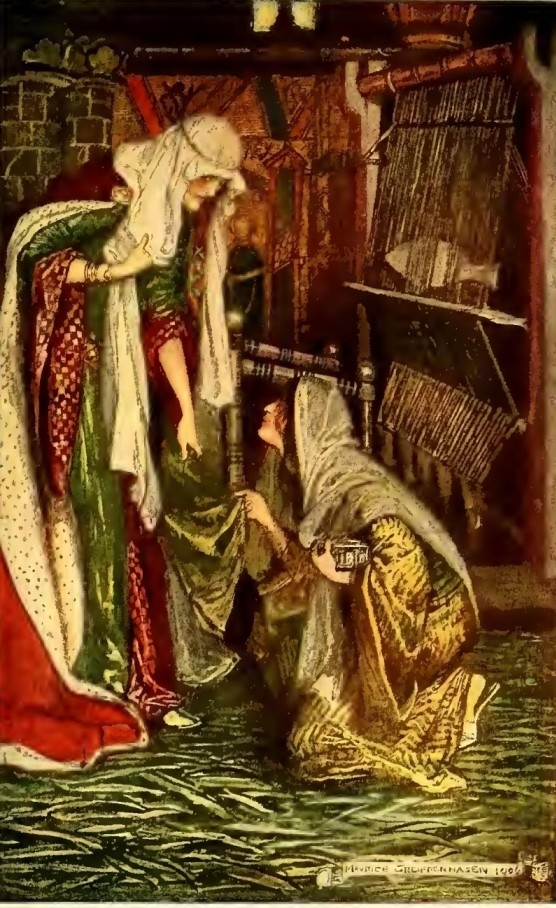
\includegraphics[height=.9\textheight]{ivanhoe/0597m}
    \caption{To the surprise of the Lady of Ivanhoe, her fair visitant
    kneeled on one knee.}
\end{figure}

``What means this, lady?'' said the surprised bride; ``or why do you
offer to me a deference so unusual?''

``Because to you, Lady of Ivanhoe,'' said Rebecca, rising up and
resuming the usual quiet dignity of her manner, ``I may lawfully, and
without rebuke, pay the debt of gratitude which I owe to Wilfred of
Ivanhoe. I am--forgive the boldness which has offered to you the homage
of my country--I am the unhappy Jewess, for whom your husband hazarded
his life against such fearful odds in the tiltyard of Templestowe.''

``Damsel,'' said Rowena, ``Wilfred of Ivanhoe on that day rendered back
but in slight measure your unceasing charity towards him in his wounds
and misfortunes. Speak, is there aught remains in which he or I can
serve thee?''

``Nothing,'' said Rebecca, calmly, ``unless you will transmit to him my
grateful farewell.''

``You leave England then?'' said Rowena, scarce recovering the surprise
of this extraordinary visit.

``I leave it, lady, ere this moon again changes. My father had a brother
high in favour with Mohammed Boabdil, King of Grenada--thither we go,
secure of peace and protection, for the payment of such ransom as the
Moslem exact from our people.''

``And are you not then as well protected in England?'' said Rowena. ``My
husband has favour with the King--the King himself is just and
generous.''

``Lady,'' said Rebecca, ``I doubt it not--but the people of England are
a fierce race, quarrelling ever with their neighbours or among
themselves, and ready to plunge the sword into the bowels of each other.
Such is no safe abode for the children of my people. Ephraim is an
heartless dove--Issachar an over-laboured drudge, which stoops between
two burdens. Not in a land of war and blood, surrounded by hostile
neighbours, and distracted by internal factions, can Israel hope to rest
during her wanderings.''

``But you, maiden,'' said Rowena--``you surely can have nothing to fear.
She who nursed the sick-bed of Ivanhoe,'' she continued, rising with
enthusiasm--``she can have nothing to fear in England, where Saxon and
Norman will contend who shall most do her honour.''

``Thy speech is fair, lady,'' said Rebecca, ``and thy purpose fairer;
but it may not be--there is a gulf betwixt us. Our breeding, our faith,
alike forbid either to pass over it. Farewell--yet, ere I go indulge me
one request. The bridal-veil hangs over thy face; deign to raise it, and
let me see the features of which fame speaks so highly.''

``They are scarce worthy of being looked upon,'' said Rowena; ``but,
expecting the same from my visitant, I remove the veil.''

She took it off accordingly; and, partly from the consciousness of
beauty, partly from bashfulness, she blushed so intensely, that cheek,
brow, neck, and bosom, were suffused with crimson. Rebecca blushed also,
but it was a momentary feeling; and, mastered by higher emotions, past
slowly from her features like the crimson cloud, which changes colour
when the sun sinks beneath the horizon.

``Lady,'' she said, ``the countenance you have deigned to show me will
long dwell in my remembrance. There reigns in it gentleness and
goodness; and if a tinge of the world's pride or vanities may mix with
an expression so lovely, how should we chide that which is of earth for
bearing some colour of its original? Long, long will I remember your
features, and bless God that I leave my noble deliverer united with--''

She stopped short--her eyes filled with tears. She hastily wiped them,
and answered to the anxious enquiries of Rowena--``I am well,
lady--well. But my heart swells when I think of Torquilstone and the
lists of Templestowe.--Farewell. One, the most trifling part of my duty,
remains undischarged. Accept this casket--startle not at its contents.''

Rowena opened the small silver-chased casket, and perceived a carcanet,
or neck lace, with ear-jewels, of diamonds, which were obviously of
immense value.

``It is impossible,'' she said, tendering back the casket. ``I dare not
accept a gift of such consequence.''

``Yet keep it, lady,'' returned Rebecca.--``You have power, rank,
command, influence; we have wealth, the source both of our strength and
weakness; the value of these toys, ten times multiplied, would not
influence half so much as your slightest wish. To you, therefore, the
gift is of little value,--and to me, what I part with is of much less.
Let me not think you deem so wretchedly ill of my nation as your commons
believe. Think ye that I prize these sparkling fragments of stone above
my liberty? or that my father values them in comparison to the honour of
his only child? Accept them, lady--to me they are valueless. I will
never wear jewels more.''

``You are then unhappy!'' said Rowena, struck with the manner in which
Rebecca uttered the last words. ``O, remain with us--the counsel of holy
men will wean you from your erring law, and I will be a sister to you.''

``No, lady,'' answered Rebecca, the same calm melancholy reigning in her
soft voice and beautiful features--``that--may not be. I may not change
the faith of my fathers like a garment unsuited to the climate in which
I seek to dwell, and unhappy, lady, I will not be. He, to whom I
dedicate my future life, will be my comforter, if I do His will.''

``Have you then convents, to one of which you mean to retire?'' asked
Rowena.

``No, lady,'' said the Jewess; ``but among our people, since the time of
Abraham downwards, have been women who have devoted their thoughts to
Heaven, and their actions to works of kindness to men, tending the sick,
feeding the hungry, and relieving the distressed. Among these will
Rebecca be numbered. Say this to thy lord, should he chance to enquire
after the fate of her whose life he saved.''

There was an involuntary tremour on Rebecca's voice, and a tenderness of
accent, which perhaps betrayed more than she would willingly have
expressed. She hastened to bid Rowena adieu.

``Farewell,'' she said. ``May He, who made both Jew and Christian,
shower down on you his choicest blessings! The bark that waits us hence
will be under weigh ere we can reach the port.''

She glided from the apartment, leaving Rowena surprised as if a vision
had passed before her. The fair Saxon related the singular conference to
her husband, on whose mind it made a deep impression. He lived long and
happily with Rowena, for they were attached to each other by the bonds
of early affection, and they loved each other the more, from the
recollection of the obstacles which had impeded their union. Yet it
would be enquiring too curiously to ask, whether the recollection of
Rebecca's beauty and magnanimity did not recur to his mind more
frequently than the fair descendant of Alfred might altogether have
approved.

Ivanhoe distinguished himself in the service of Richard, and was graced
with farther marks of the royal favour. He might have risen still
higher, but for the premature death of the heroic Coeur-de-Lion, before
the Castle of Chaluz, near Limoges. With the life of a generous, but
rash and romantic monarch, perished all the projects which his ambition
and his generosity had formed; to whom may be applied, with a slight
alteration, the lines composed by Johnson for Charles of Sweden--

\begin{verse}
His fate was destined to a foreign strand,\\
A petty fortress and an ``humble'' hand;\\
He left the name at which the world grew pale,\\
To point a moral, or adorn a \textsc{tale}.\\!
\end{verse}


    \backmatter
    \appendix
    \section[Descriptive Notes]{
    
\includegraphics[width=9.3cm]{viking-tales/046}}

\phantomsection\label{house}
\emph{House.} In a rich Norseman's home were many buildings. The finest
and largest was the great feast hall. Next were the bower, where the
women worked, and the guest house, where visitors slept. Besides these
were storehouses, stables, work-shops, a kitchen, a sleeping-house for
thralls. All these buildings were made of heavy, hewn logs, covered with
tar to fill the cracks and to keep the wood from rotting. The ends of
the logs, the door-posts, the peaks of gables, were carved into shapes
of men and animals and were painted with bright colors. These gay
buildings were close together, often set around the four sides of a
square yard. That yard was a busy and pleasant place, with men and women
running across from one bright building to another. Sometimes a high
fence with one gate went around all this, and only the tall, carved
peaks of roofs showed from the outside.

\phantomsection\label{names}
\noindent\emph{Names.} An old Norse story says: ``Most men had two names
in one, and thought it likeliest to lead to long life and good luck to
have double names.'' To be called after a god was very lucky. Here are
some of those double names with their meanings: ``Thorstein'' means
Thor's stone; ``Thorkel'' means Thor's fire; ``Thorbiorn'' means Thor's
bear; ``Gudbrand'' means Gunnr's sword (Gunnr was one of the
Valkyrias\footnote{See note about Valkyrias on
page~\pageref{valkyrias}.}); ``Gunnbiorn'' means Gunnr's bear; ``Gudrid''
means Gunnr's rider; ``Gudrod'' means Gunnr's land-clearer. (Most of the
land in old Norway was covered with forests. When a man got new land he
had to clear off the trees.) In those olden days a man did not have a
surname that belonged to everyone in his family. Sometimes there were
two or three men of the same name in a neighborhood. That caused
trouble. People thought of two ways of making it easy to tell which man
was being spoken of. Each was given a nickname. Suppose the name of each
was Haki. One would be called Haki the Black because he had black hair.
The other would be called Haki the Ship-chested because his chest was
broad and strong. These nicknames were often given only for the fun of
it. Most men had them,--Eric the Red, Leif the Lucky, Harald Hairfair,
Rolf Go-afoot. The other way of knowing one Haki from the other was to
tell his father's name. One was Haki, Eric's son. The other was Haki,
Halfdan's son. If you speak these names quickly, they sound like Haki
Ericsson and Haki Halfdansson. After a while they were written like
that, and men handed them on to their sons and daughters. Some names
that we have nowadays have come down to us in just that way--Swanson,
Anderson, Peterson, Jansen. There was another reason for these last
names: a man was proud to have people know who his father was.

\phantomsection\label{drinking-horns}
\noindent\emph{Drinking-horns.} The Norsemen had few cups or goblets.
They used instead the horns of cattle, polished and trimmed with gold or
silver or bronze. They were often very beautiful, and a man was almost as
proud of his drinking-horn as of his sword.

\phantomsection\label{tables}
\noindent\emph{Tables.} Before a meal thralls brought trestles into the
feast hall and set them before the benches. Then they laid long boards
across from trestle to trestle. These narrow tables stretched all along
both sides of the hall. People sat at the outside edge only. So the
thralls served from the middle of the room. They put baskets of bread and
wooden platters of meat upon these bare boards. At the end of the meal
they carried out tables and all, and the drinking-horns went round in a
clean room.

\phantomsection\label{beds}
\noindent\emph{Beds.} Around the sides of the feast hall were shut-beds.
They were like big boxes with doors opening into the hall. On the floor
of this box was straw with blankets thrown over it. The people got into
these beds and closed the doors and so shut themselves in. Olaf's men
could have set heavy things against these doors or have put props
against them. Then the people could not have got out; for on the other
side of the bed was the thick outside wall of the feast hall, and there
were no windows in it.

\phantomsection\label{feast-hall}
\noindent\emph{Feast Hall.} The feast hall was long and narrow, with a
door at each end. Down the middle of the room were flat stones in the
dirt floor. Here the fires burned. In the roof above these fires were
holes for the smoke to go out, but some of it blew about the hall, and
the walls and rafters were stained with it. But it was pleasant wood
smoke, and the Norsemen did not dislike it. There were no large windows
in a feast hall or in any other Norse building. High up under the eaves
or in the roof itself were narrow slits that were called wind's-eyes.
There was no glass in them, for the Norsemen did not know how to make it;
but there were, instead, covers made of thin, oiled skin. These were put
into the wind's-eyes in stormy weather. There were covers, too, for the
smoke-holes. The only light came through these narrow holes, so on dark
days the people needed the fire as much for light as for warmth.

\phantomsection\label{foster-father}
\noindent\emph{Foster-father.} A Norse father sent his children away from
home to grow up. They went when they were three or four years old and
stayed until they were grown. The father thought: ``They will be better
so. If they stayed at home, their mother would spoil them with much
petting.''

\phantomsection\label{foster-brothers}
\noindent\emph{Foster-brothers.} When two men loved each other very much
they said, ``Let us become foster-brothers.''

Then they went and cut three long pieces of turf and put a spear into
the ground so that it held up the strips of turf like an arch. Runes
were cut on the handle of the spear, telling the duties of
foster-brothers. The two men walked under this arch, and each made a
little cut in his palm. They knelt and clasped hands, so that the blood
of the two flowed together, and they said, ``Now we are of one blood.''

Then each made this vow: ``I will fight for my foster-brother whenever
he shall need me. If he is killed before I am, I will punish the man who
did it. Whatever things I own are as much my foster-brother's as mine. I
will love this man until I die. I call Odin and Thor and all the gods to
hear my vow. May they hate me if I break it!''

\phantomsection\label{ran}
\noindent\emph{Ran.} Ran was the wife of Aegir, who was god of the sea.
They lived in a cave at the bottom of the ocean. Ran had a great net, and
she caught in it all men who were shipwrecked and took them to her cave.
She also caught all the gold and rich treasures that went down in ships.
So her cave was filled with shining things.

\phantomsection\label{valkyrias}
\noindent\emph{Valkyrias.} These were the maidens of Odin. They waited
on the table in Valhalla. But whenever a battle was being fought they
rode through the air on their horses and watched to see what warriors
were brave enough to go to Valhalla. Sometimes during the fight a man
would think that he saw the Valkyrias. Then he was glad; for he knew that
he would go to Valhalla.

An old Norse story says this about the Valkyrias: ``With lightning
around them, with bloody shirts of mail, and with shining spears they
ride through the air and the ocean. When their horses shake their manes,
dew falls on the deep valleys and hail on the high forests.''

\phantomsection\label{odins-ravens}
\noindent\emph{Odin's Ravens.} Odin had a great throne in his palace in
Asgard. When he sat in it he could look all over the world. But it was so
far to see that he could not tell all of the things that were happening.
So he had two ravens to help him. An old Norse story tells this about
them: ``Two ravens sit on Odin's shoulders and whisper in his ears all
that they have heard and seen. He sends them out at dawn of day to see
over the whole world. They return at evening near meal time. This is why
Odin knows so many things.''

\phantomsection\label{reykjavik}
\noindent\emph{Reykjavik.} Reykjavik means ``smoky sea.'' Ingolf called
it that because of the steaming hot-springs by the sea. The place is
still called Reykjavik. A little city has grown up there, the only city
in Iceland. It is the capital of the country.

\phantomsection\label{peace-bands}
\noindent\emph{Peace-bands.} A Norseman always carried his sword, even at
a feast; for he did not know when he might need it. But when he went
somewhere on an errand of peace and had no quarrel he tied his sword
into its scabbard with white bands that he called peace-bands. If all at
once something happened to make him need his sword, he broke the
peace-bands and drew it out.

\phantomsection\label{eskimos}
\noindent\emph{Eskimos.} Now, the Eskimos live in Greenland and Alaska
and on the very northern shores of Canada. But once they lived farther
south in pleasanter lands. After a while the other Indian tribes began to
grow strong. Then they wanted the pleasant land of the Eskimos and the
seashore that the Eskimos had. So they fought again and again with those
people and won and drove them farther north and farther north. At last
the Eskimos were on the very shores of the cold sea, with the Indians
still pushing them on. So some of them got into their boats and rowed
across the narrow water and came to Greenland and lived there. Some
people think that these things happened before Eric found Greenland. In
that case he found Eskimos there; and Thorfinn saw red Indians in
Wineland. Other people think that this happened after Eric went to
Greenland. If that is true, he found an empty land, and it was Eskimos
that Thorfinn saw in Wineland.

\section[Suggestions to Teachers]{
    
\includegraphics[width=9.3cm]{viking-tales/047}}

\lettrine{P}{ossibly} this book seems made up of four or five
disconnected stories. They are, however, strung upon one thread,--the
westward emigration from Norway. The story of Harald is intended to serve
in two ways towards the working out of this plot. It gives the general
setting that continues throughout the book in costume, houses, ideals,
habits. It explains the cause of the emigration from the mother country.
It is really an introductory chapter. As for the other stories, they are
distinctly steps in the progress of the plot. A chain of islands loosely
connects Norway with America,--Orkneys and Shetlands, Faroes, Iceland,
Greenland. It was from link to link of this chain that the Norsemen
sailed in search of home and adventure. Discoveries were made by
accident. Ships were driven by the wind from known island to unknown.
These two points,--the island connection that made possible the long
voyage from Norway to America, and the contribution of storm to
discovery,--I have stated in the book only dramatically. I emphasize them
here, hoping that the teacher will make sure that the children see them,
and possibly that they state them abstractly.

Let me speak as to the proper imaging of the stories. I have not often
interrupted incident with special description, not because I do not
consider the getting of vivid and detailed images most necessary to full
enjoyment and to proper intellectual habits, but because I trusted to
the pictures of this book and to the teacher to do what seemed to me
inartistic to do in the story. Some of these descriptions and
explanations I have introduced into the book in the form of notes,
hoping that the children in turning to them might form a habit of
insisting upon full understanding of a point, and might possibly, with
the teacher's encouragement, begin the habit of reference reading.

The landscape of Norway, Iceland, and Greenland is wonderful and will
greatly assist in giving reality and definiteness to the stories.
Materials for this study are not difficult of access. Foreign colored
photographs of Norwegian landscape are becoming common in our art
stores. There are good illustrations in the geographical works referred
to in the book list. These could be copied upon the blackboard. There
are three books beautifully illustrated in color that it will be
possible to find only in large libraries,--``Coast of Norway,'' by
Walton; ``Travels in the Island of Iceland,'' by Mackenzie; ``Voyage en
Islande et au Gröenland,'' by J. P. Gaimard. If the landscape is studied
from the point of view of formation, the images will be more accurate
and more easily gained, and the study will have a general value that
will continue past the reading of these stories into all work in
geography.

Trustworthy pictures of Norse houses and costumes are difficult to
obtain. In ``Viking Age'' and ``Story of Norway,'' by Boyesen (G. P.
Putnam's Sons, New York), are many copies of Norse antiquities in the
fashion of weapons, shield-bosses, coins, jewelry, wood-carving. These
are, of course, accurate, but of little interest to children. Their
chief value lies in helping the teacher to piece together a picture that
she can finally give to her pupils.

Metal-working and wood-carving were the most important arts of the
Norse. If children study products of these arts and actually do some of
the work, they will gain a quickened sympathy with the people and an
appreciation of their power. They may, perhaps, make something to merely
illustrate Norse work; for instance, a carved ship's-head, or a copper
shield, or a wrought door-nail. But, better, they may apply Norse ideas
of form and decoration and Norse processes in making some modern thing
that they can actually use; for instance, a carved wood pin-tray or a
copper match holder. This work should lead out into a study of these
same industries among ourselves with visits to wood-working shops and
metal foundries.

Frequent drawn or painted illustration by the children of costumes,
landscapes, houses, feast halls, and ships will help to make these
images clear. But dramatization will do more than anything else for the
interpreting of the stories and the characters. It would be an excellent
thing if at last, through the dramatization and the handwork, the
children should come into sufficient understanding and enthusiasm to
turn skalds and compose songs in the Norse manner. This requires only a
small vocabulary and a rough feeling for simple rhythm, but an intensity
of emotion and a great vividness of image.

These Norse stories have, to my thinking, three values. The men, with
the crude courage and the strange adventures that make a man interesting
to children, have at the same time the love of truth, the hardy
endurance, the faithfulness to plighted word, that make them a child's
fit companions. Again, in form and in matter old Norse literature is
well worth our reading. I should deem it a great thing accomplished if
the children who read these stories should so be tempted after a while
to read those fine old books, to enjoy the tales, to appreciate
straightforwardness and simplicity of style. The historical value of the
story of Leif Ericsson and the others seems to me to be not to learn the
fact that Norsemen discovered America before Columbus did, but to gain a
conception of the conditions of early navigation, of the length of the
voyage, of the dangers of the sea, and a consequent realization of the
reason for the fact that America was unknown to mediæval Europe, of why
the Norsemen did not travel, of what was necessary to be done before men
should strike out across the ocean. Norse story is only one chapter in
that tale of American discovery. I give below an outline of a year's
work on the subject that was once followed by the fourth grade of the
Chicago Normal School. The idea in it is to give importance, sequence,
reasonableness, broad connections, to the discovery of America.

The head of the history department who planned this course says it is
``in a sense a dramatization of the development of geographical
knowledge.''

Following is a bare topical outline of the work:

\begin{itemize}
\item Evolution of the forms of boats.
\item Viking tales.
\item A crusade as a tale of travel and discovery.
\item Monasteries as centers of work.
\item Printing.
\item Story of Marco Polo.
\item Columbus' discovery.
\item Story of Vasco da Gama.
\item Story of Magellan.
\end{itemize}

\begin{figure}[hb]
    \centering
    \vskip8pt
    
\includegraphics[width=2.7cm]{viking-tales/014}
\end{figure}

\section[A Reading List]{
    
\includegraphics[width=9.3cm]{viking-tales/048}}

\subsection*{Geography}

NORWAY: ``The Earth and Its Inhabitants,'' Reclus. \emph{D. Appleton \&
Co., New York.}

\noindent ICELAND: ``The Earth and Its Inhabitants,'' ``Iceland,''
Baring-Gould. \emph{Smith, Elder \& Co., London, 1863.}

\begin{itemize}
\item ``Iceland, Greenland, and the Faroes.'' \emph{Harper Bros., New York.}
\item ``An American in Iceland,'' Kneeland. \emph{Lockwood, Brooke \& Co., Boston,
1876.}
\end{itemize}

\noindent GREENLAND: ``The Earth and Its Inhabitants,'' Reclus. \emph{D.
Appleton \& Co., New York.}

\begin{itemize}
\item ``Iceland, Greenland, and the Faroes.'' \emph{Harper Bros., New York.}
\end{itemize}

\subsection*{Customs}

``Viking Age,'' Du Chaillu. \emph{Charles Scribner's Sons, 1889.}

\noindent``Private Life of the Old Northmen,'' Keyser; translated by
Barnard. \emph{Chapman \& Hall, London, 1868.}

\noindent ``Saga Time,'' Vicary. \emph{Kegan Paul, Trench, Trübner \&
Co., London.}

\noindent ``Story of Burnt Njal'' (Introduction), Dasent. \emph{Edmonston
\& Douglas, Edinburgh, 1861.}

\noindent ``Vikings of the Baltic, a romance;'' Dasent. \emph{Edmonston
\& Douglas, Edinburgh.}

\noindent ``Ivar the Viking, a romance;'' Du Chaillu. \emph{Charles
Scribner's Sons, New York.}

\noindent ``Viking Path, a romance;'' Haldane Burgess. \emph{Wm.
Blackwood \& Sons, Edinburgh, 1894.}

\noindent ``Northern Antiquities,'' Percy, edited by Blackwell.
\emph{Bohn, London, 1859.}

\noindent Also the Sagas named on page 206.

\subsection*{Mythology}

The Prose Edda, ``Northern Antiquities,'' Percy, edited by Blackwell.
\emph{Bohn, London, 1859.}

\noindent ``Norse Mythology,'' Anderson. \emph{Scott, Foresman \& Co.,
Chicago, 1876.}

\noindent ``Norse Stories,'' Mabie. \emph{Rand, McNally \& Co., Chicago,
1902.}

\noindent ``Northern Mythology,'' Thorpe. \emph{Lumley, London, 1851.}

\noindent ``Classic Myths,'' Judd. \emph{Rand, McNally \& Co., Chicago,
1902.}

\subsection*{Incidents}

HARALD: Saga of Harald Hairfair, in ``Saga Library,'' Magnusson and
Morris, Vol. I. \emph{Bernard Quaritch, London; Charles Scribner's Sons,
New York, 1892.}

\noindent INGOLF: ``Norsemen in Iceland,'' Dasent in Oxford Essays, Vol.
IV. \emph{Parker \& Son, London, 1858.}

\begin{itemize}
\item ``Iceland, Greenland, and the Faroes.'' \emph{Harper Bros., New York.}
\item ``A Winter in Iceland and Lapland,'' \emph{Dillon. Henry Colburn, London,
1840.}
\end{itemize}

\noindent ERIC, LEIF, AND THORFINN: ``The Finding of Wineland the Good,''
Reeves. \emph{Henry Froude, 1890.}

\begin{itemize}
\item ``America Not Discovered by Columbus.'' Anderson. \emph{Scott, Foresman \&
Co., Chicago, 1891.}
\end{itemize}

\subsection*{Credibility of Story}

Winsor's ``Narrative and Critical History of America,'' Vol. I. \emph{C.
A. Nichols Co., Springfield, Mass., 1895.}

\noindent ``Discovery of America,'' Fiske, Vol. I. \emph{Houghton,
Mifflin \& Co., Boston, 1892.}

\subsection*{Other Sagas Easily Accessible}

``Saga Library,'' 5 vols.; Morris and Magnusson. \emph{Bernard Quaritch,
London; Charles Scribner's Sons, New York, 1892.} As follows:

\begin{itemize}
\item ``The Story of Howard the Halt,'' ``The Story of the Banded Men,'' ``The
Story of Hen Thorir.'' Done into English out of Icelandic by William
Morris and Eirikr Magnusson.
\item ``The Story of the Ere-dwellers,'' with ``The Story of the
Heath-slayings'' as Appendix. Done into English out of the Icelandic
by William Morris and Eirikr Magnusson.
\item ``The Stories of the Kings of Norway, called the Round World''
(Heimskringla). By Snorri Sturluson. Done into English by William
Morris and Eirikr Magnusson. With a large map of Norway. In three
volumes.
\end{itemize}

\noindent ``Gisli the Outlaw,'' Dasent. \emph{Edmonston \& Douglas,
Edinburgh.}

\noindent ``Orkneyinga Saga,'' Anderson. \emph{Edmonston \& Douglas,
Edinburgh.}

\noindent ``Volsunga Saga,'' Morris and Magnusson. \emph{Walter Scott,
London.}

\noindent ``The Younger Edda,'' Anderson. \emph{Scott, Foresman \& Co.,
Chicago, 1880.}

\noindent (A full bibliography of the Sagas may be found in ``Volsunga
Saga.'')

\begin{figure}[hb]
    \centering
    \vskip8pt
    
\includegraphics[width=2.7cm]{viking-tales/011}
\end{figure}

\section[A Pronouncing Index]{
    
\includegraphics[width=9.3cm]{viking-tales/049}}

(\emph{This index and guide to pronunciation which are given to indicate
the pronunciation of the more difficult words, are based upon the 1918
edition of Webster's New International Dictionary.})

\noindent\textbf{Transcriber's Note:}\\
Minor typographical errors have been corrected without note. The up tack
diacritical mark over a vowel is represented by [+a], [+e], [+i] and
[+o].

\begin{multicols}{3}
\noindent\textbf{Aegir} (ē´ jĭr)\\
\textbf{\emph{Ȧ}rā´ bĭ \emph{ȧ}}\\
\textbf{Ärn´ vĭd}\\
\textbf{Ăs´ gärd}\\
\textbf{A̤ud´ bĭ ôrn}\\
\textbf{A̤u´dŭn}

\noindent\textbf{Bĭ är´ nĭ}

\noindent\textbf{Eric} (ē´ rĭk)\\
\textbf{Ericsson} (ĕr´ ĭk s\emph{ŭ}n)
\textbf{Eyjolf} (ī´ y{[}+o{]}lf)

\noindent\textbf{Faroes} (fā´ rōz)\\
\textbf{fiord} (fyôrd)\\
\textbf{Flō´ kĭ}

\noindent\textbf{Grĭm}\\
\textbf{Gŭd´ bränd}\\
\textbf{Gŭd´ rĭd}\\
\textbf{Gŭd´ rōd}\\
\textbf{Gŭn\emph{n}´ bĭ ôrn}\\
\textbf{Gṳ´ t\emph{h}ôrm}\\
\textbf{Gyda} (gē´ d{[}+a{]})

\noindent\textbf{Hä´ kĭ}\\
\textbf{Hä´ k{[}+o{]}n}\\
\textbf{Hälf´ dăn}\\
\textbf{Hăr´ ăld}\\
\textbf{Hä´ värd}\\
\textbf{Hĕl´ ä}\\
\textbf{Hĕl´ g{[}+a{]}}\\
\textbf{Hẽr´ st\emph{e}īn}\\
\textbf{Holmstein} (hōlm´ stīn)

\noindent\textbf{Ĭn´ gôlf}\\
\textbf{Ī´ vär}

\noindent\textbf{Leif} (l{[}+i{]}f)

\noindent\textbf{Niflheim} (n{[}+e{]}v´ 'l hām)

\noindent\textbf{Ō´ dĭn}\\
\textbf{Ō´ läf}\\
\textbf{Orkneys} (ôrk´ nĭz)

\noindent\textbf{Rän}\\
\textbf{Reykjavik} (rā´ ky\emph{ȧ} vēk´)\\
\textbf{Rôlf}

\noindent\textbf{Shĕt´ l\emph{ă}nds}\\
\textbf{Sif} (sēf)\\
\textbf{Sighvat} (sĭg´ văt)\\
\textbf{Snorri} (snŏr´ r{[}+e{]})\\
\textbf{Sôl´ fĭ}

\noindent\textbf{Thor (thôr)}\\
\textbf{T\emph{h}ôr´ bĭ ôrn}\\
\textbf{T\emph{h}ôr´ fĭnn}\\
\textbf{T\emph{h}ôr´ gĕst}\\
\textbf{T\emph{h}ôr´hĭld}\\
\textbf{T\emph{h}ôr´ kĕl}\\
\textbf{T\emph{h}ôr´ l\emph{e}īf}\\
\textbf{T\emph{h}ôr´ ôlf}\\
\textbf{T\emph{h}ôr´ st\emph{e}īn}\\
\textbf{Tyrker} (tẽr´ kẽr)

\noindent\textbf{Văl hăl´ \emph{lȧ}}\\
\textbf{Valkyria} (văl kĭr´ \emph{yȧ})\\
\textbf{Vī´ kĭng}
\end{multicols}

\subsection*{A Guide to Pronunciation}

\begin{multicols}{3}
\noindent\textbf{ā} as in \textbf{āle}\\
\textbf{ă} as in \textbf{ădd}\\
\textbf{\emph{ă}} as in \textbf{fin\emph{ă}l}\\
\textbf{ȧ} as in \textbf{ȧsk}\\
\textbf{\emph{ȧ}} as in \textbf{sof\emph{ȧ}}\\
\textbf{ä} as in \textbf{ärm}\\
\textbf{a̤} as in \textbf{a̤ll}

\noindent\textbf{ē} as in \textbf{ēve}\\
\textbf{{[}+e{]}} as in \textbf{{[}+e{]}vent´}\\
\textbf{ĕ} as in \textbf{ĕnd}\\
\textbf{ẽ} as in \textbf{hẽr}

\noindent\textbf{ī} as in \textbf{īce}\\
\textbf{ĭ} as in \textbf{ĭt}

\noindent\textbf{ō} as in \textbf{ōld}\\
\textbf{{[}+o{]}} as in \textbf{{[}+o{]}bey´}\\
\textbf{ŏ} as in \textbf{ŏdd}\\
\textbf{ô} as in \textbf{lôrd}

\noindent\textbf{ŭ} as in \textbf{ŭp}\\
\textbf{\emph{ŭ}} as in \textbf{circ\emph{ŭ}s}\\
\textbf{ṳ} as in \textbf{rṳde}

\noindent\textbf{ȳ} as in \textbf{flȳ}
\end{multicols}

\noindent Silent letters are italicized.

    \fulllicense

\end{document}
